\documentclass{IEEEoj}
\usepackage[table,xcdraw]{xcolor}
\usepackage{cite}
\usepackage{amsmath,amssymb,amsfonts}
\usepackage{algorithmic}
\usepackage{graphicx,color}
\usepackage{textcomp}
\usepackage{glossaries}
\usepackage{multirow}
\usepackage{url}
\usepackage{comment}
\usepackage[utf8]{inputenc}
\usepackage{pgfplots}
\usepackage{afterpage}
\usepackage{orcidlink}
\usepackage{ulem} 
\usepackage{soul}
\pgfplotsset{compat=newest}
\usepackage{tikz}
%\tikzset{external/export=false}
\usetikzlibrary{external,patterns,shapes.arrows}
%\tikzexternalize[prefix=IEEE_OJCOMS-template-LaTex_202401/tikz/]
\DeclareUnicodeCharacter{2212}{−}
\usepgfplotslibrary{groupplots,dateplot}
\usepackage{adjustbox}


\newcommand{\rev}[1]{\textcolor{black}{#1}}



% acronyms go here

\newacronym{av}{AV}{autonomous vehicle}
\newacronym{nn}{NN}{neural network}
\newacronym{tsp}{TSP}{Travelling Salesman problem}
\newacronym{vrp}{VRP}{Vehicle Routing Problem}
\newacronym{cvrp}{CVRP}{Capacitated Vehicle Routing Problem}
\newacronym{rl}{RL}{reinforcement learning}
\newacronym{gnn}{GNN}{Graph Neural Net}
\newacronym{gat}{GAT}{Graph Attention Net}
\newacronym{rnn}{RNN}{Recurrent Neural Net}
\newacronym{drl}{DRL}{Deep Reinforcement Learning}
\newacronym{mlp}{MLP}{Multi-Layer Perceptron}

\newacronym{co}{CO}{Combinatorial Optimization}
\newacronym{ndp}{TNDP}{Transit Network Design Problem}
\newacronym{fsp}{FSP}{Frequency-Setting Problem}
\newacronym{dfsp}{DFSP}{Design and Frequency-Setting Problem}
\newacronym{sp}{SP}{Scheduling Problem}
\newacronym{tp}{TP}{Timetabling Problem}
\newacronym{ndsp}{NDSP}{Network Design and Scheduling Problem}

\newacronym{mod}{MoD}{Mobility on Demand}
\newacronym{amod}{AMoD}{Autonomous Mobility on Demand}
\newacronym{imodp}{IMoDP}{Intermodal Mobility-on-Demand Problem}
\newacronym{matsim}{MATSim}{Multi-Agent Transport Simulation}
\newacronym{od}{OD}{Origin-Destination}
\newacronym{csa}{CSA}{Connection Scan Algorithm}
\newacronym{mdp}{MDP}{Markov Decision Process}
\newacronym{dqn}{DQN}{Deep Q-Networks}
\newacronym{acer}{ACER}{Actor-Critic with Experience Replay}
\newacronym{ppo}{PPO}{Proximal Policy Optimization}
\newacronym{artm}{ARTM}{Metropolitan Regional Transportation Authority}
\newacronym{stl}{STL}{Soci\'et\'e de Transport de Laval}
\newacronym{cda}{CDA}{Census Dissemination Area}

\def\BibTeX{{\rm B\kern-.05em{\sc i\kern-.025em b}\kern-.08em
    T\kern-.1667em\lower.7ex\hbox{E}\kern-.125emX}}
\AtBeginDocument{\definecolor{ojcolor}{cmyk}{0.93,0.59,0.15,0.02}}
\def\OJlogo{\vspace{-4pt}\hskip-4pt}
\bibliographystyle{ieeetr}

\begin{document}
\title{A Slicing Model for Transport Networks with Traffic Burst Control and QoS Compliance for Traffic Flows}

\author{Aitor Encinas-Alonso\IEEEauthorrefmark{1}\orcidlink{0009-0000-1290-8815}, Carlos M. Lentisco\IEEEauthorrefmark{1}\orcidlink{0000-0002-7444-0872}, Ignacio Soto\IEEEauthorrefmark{1}\orcidlink{0000-0002-7421-3733 }, Luis Bellido\IEEEauthorrefmark{1}\orcidlink{0000-0001-9591-0928}, David Fernandez\IEEEauthorrefmark{1}\orcidlink{0000-0002-2172-9162}
}
\affil{Departamento de Ingeniería de Sistemas Telemáticos, ETSI Telecomunicación, Universidad Politécnica de Madrid, Spain}
\corresp{CORRESPONDING AUTHOR: Aitor Encinas-Alonso (e-mail: aitor.encinas.alonso@alumnos.upm.es).}
\authornote{This work was partially supported by the Remote Driver project (TSI-065100-2022-003) funded by the Ministerio de Asuntos Económicos y Transformación Digital (Gobierno de España) and the European Union's Horizon Europe research and innovation program under Grant Agreement No. 101097122 (ACROSS).}
\markboth{Preparation of Papers for IEEE OPEN JOURNALS}{Author \textit{et al.}}


\begin{abstract}
Network slicing has emerged as a key network technology, providing network operators with the means to offer virtual networks to vertical users over a single physical network infrastructure. Recent research has resulted mainly in techniques for managing and deploying network slices, but the implementation of network slices on a real physical transport network infrastructure has received much less attention. Standardization bodies, such as the \gls{ietf}, have provided some implementation recommendations. Still, there is a lack of mechanisms to implement network slices capable of handling traffic bursts while simultaneously meeting the \gls{qos} requirements of the traffic flows associated with the slices. In this paper, we propose a novel fine-grained resource control mechanism to implement transport network slices that meet traffic \gls{qos} requirements while both accepting limited traffic bursts, and enabling efficient bandwidth sharing within and across slices. The mechanism is executed at the edge of the transport network. The proposed model aligns with current standards on network slicing and has been tested on an experimental platform. Using this platform, we have conducted an extensive experimental campaign that demonstrates that our proposal can effectively control traffic bursts generated within the network slices while maximizing bandwidth utilization across the network.
\end{abstract}

\begin{IEEEkeywords}
Network Slicing, Quality of Service, Communication System Traffic Control,  Mobile Communication, Transport Network.
\end{IEEEkeywords}

\maketitle

\section{Introduction}
\label{sec:intro}
Although the deployment of commercial 5G networks is a reality in many countries worldwide, the most advanced features proposed in the \gls{3gpp} 5G standards are still under investigation. Among them, network slicing promises to revolutionize the way in which network infrastructures are exploited. With network slicing, a network infrastructure can be shared to provide different and isolated network services~\cite{3GPP2024_1}. Network slicing allows network operators to provide different communication services with tailored quality levels. Examples are \gls{urllc}, \gls{embb}, or \gls{miot}. Network slicing techniques can be applied to the different segments that compose a mobile network: the \gls{ran}, the \gls{tn}, and \gls{cn}. While the \gls{ran} and \gls{cn} fall under the domain of \gls{3gpp}, the \gls{tn} belongs to the \gls{ietf}'s domain. A mobile network operator may predefine a set of network slices, allowing external customers to subscribe to the communication services that best suit their applications. Additionally, operators can enable customers to define their own network slices based on specific needs. Vertical industries are expected to be one of the main beneficiaries of network slicing, obtaining customized connectivity services through a shared network infrastructure. 

Up to this date, the state of the art has focused on the problem of allocating network resources to different network slices efficiently, especially in the \gls{ran} segment of the network. Regarding the transport network, the \gls{ietf} has defined models for controlling the allocation of resources to different network slices, but these models do not provide the ability to limit the impact on the \gls{qos} of the traffic associated with services delivered over such slices. 
%\rev{In the literature, network slicing models have been defined that provide mechanisms to guarantee bandwidth and delay for slices, with some proposals even including mechanisms for burst traffic control. However, none of these models integrate all these capabilities in a cohesive manner. This paper advances in this direction by proposing \gls{hctns}, a model for transport network slicing that efficiently manage the available bandwidth while fulfilling service \gls{qos} requirements. The  results demonstrate that our proposal achieves better outcomes in reducing the delay of flows associated with slices and enhances resource utilization when these are shared among different slices. Furthermore, it integrates a burst traffic control mechanism in a unified manner.} This paper advances in this direction by proposing \gls{hctns}, a network slicing model for transport networks that efficiently manage the available bandwidth while fulfilling service \gls{qos} requirements. 

Our proposal is applied to a scenario where standard network slices such as \gls{urllc} and \gls{embb} 
are sharing the physical network infrastructure with a network slice for \gls{tod}. \gls{tod} is an advanced automotive industry use case that enables drivers to operate vehicles remotely~\cite{Amador2022}. 

%\sout{\rev{Originally designed to assist autonomous driving in situations where vehicles cannot make decisions independently, \gls{tod} has gained interest from sectors such as public and logistic transportation as a standalone service.}}

In our target scenario, a \gls{tod} service provider signs a contract with an operator of a public mobile network to hire a network slice for the \gls{tod} service. Within the \gls{tod} service, various traffic flows with different \gls{qos} requirements (video, telemetry, and commands) are generated. Consequently, the network slice for \gls{tod} must be capable of providing differentiated traffic treatment for each type of traffic flow within the slice. 


The main contributions of this work are:
\begin{itemize}

\item The design of a flexible slicing model for transport networks, named \gls{hctns}, aligned with current \gls{ietf} standards, enhancing bandwidth sharing between traffic classes and slices while providing explicit control over how bandwidth is allocated. The model also ensures consistent \gls{qos} behavior for all traffic accepted in the \gls{tn} within the same traffic class, or, in its absence, within the same slice.

\item \gls{hctns} incorporates a novel traffic policer that optimizes the utilization of available bandwidth both across slices and within individual slices. 

\item A new traffic burst control mechanism that enables the network to accommodate traffic bursts while managing their impact on the \gls{qos} experienced by the different traffic flows in the \gls{tn} through configurable parameters.

\item A performance evaluation, based on an implemented prototype, showing that by applying our proposal it is possible to meet the strict \gls{qos} requirements of services such as \gls{tod}. The results confirm the advantages of \gls{hctns} in ensuring that all traffic flows within any network slice adhere to the defined \gls{qos} requirements. \rev{Moreover, the experiments show that our proposal outperforms the 5G transport network slicing model that is being standardized by the IETF and a reference proposal in the literature.}
\end{itemize}

The remainder of the paper is organized as follows. Section~\ref{sec:soa} reviews the related work and highlights the contributions of this paper to the state of the art.
Section~\ref{sec:background} describes the IETF 5G transport network slicing model, which serves as the reference model for our proposed work. 
Section~\ref{sec:proposal} describes the \gls{hctns} network slicing and QoS model.
Section~\ref{sec:eval} presents our testbed with a simplified version of our proposed network slicing model for 5G transport networks, configured to support teleoperated driving services sharing the same physical network with other typical and constrained slices. This section is also dedicated to the evaluation of the proposal. Finally,  Section~\ref{sec:conclusion} summarizes the main conclusions of our work. 

\rev{A summary of key acronyms used in the article is presented in Table~\ref{table:acronyms}.}

\begin{table}[tbh]
\centering
\begin{tabular}{ |l l| } 
\hline
\rowcolor{lightgray} Acronym & Definition \\
\hline
\hline
5QI & 5G Quality Indicator \\
BE & Best Effort \\
CBS & Committed Burst Size \\
CIR & Committed Information Rate \\
DRR & Deficit Round Robin \\
DSCP & Differentiated Services Code Point \\
eMBB & enhanced Mobile Broadband \\
HCTNS & Hierarchically Controlled Transport Network Slicing \\
HTB & Hierarchical Token Bucket \\
PBS & Peak Burst Size \\
PDB & Packet Delay Budget \\
PE & Provider Edge \\
PHB & Per-Hop-Behaviour \\
PIR & Peak Information Rate \\
PQ & Priority Queue \\
S-NSSAI & Single - Network Slice Selection Assistance Information \\
SDP & Service Demarcation Point \\
SLA & Service Level Agreement \\
SR & Segment Routing \\
SRH & Segment Router Header \\
TC & Traffic Control \\
TE & Traffic Engineering \\
TN & Transport Network \\
ToD & Teleoperated Driving \\
trTCM & two rate Three Color Marker \\
TS & Technical Specification \\
UPF & User Plane Function \\
URLLC & Ultra Reliable Low Latency Communications \\
VLAN & Virtual Local Area Network \\
VNX & Virtual Networks over LinuX \\
WFQ & Weighted Fair Queuing \\
\hline
\end{tabular}
\vspace*{0.25cm}
\caption{\rev{Summary of important acronyms.}}
\label{table:acronyms}
\end{table}

\section{Related Work}
\label{sec:soa}
\subsection{Network Slicing Standards}
\label{subsec:soa-standards}
The \gls{3gpp} has done a great deal of standardization work on network slicing and \gls{qos} in 5G. \gls{ts} 23.501 \cite{3GPP2023_1} defines the overall 5G system architecture, including a framework providing \gls{qos} to network flows and an identification mechanism for managing network slices. 

\gls{ts} 28.530~\cite{3GPP2024_1} defines the general concepts and definitions for network slicing, as well as the phases that compose the lifecyle of a network slice instance. \gls{ts} 23.502~\cite{3GPP2023_2} describes the procedures to define the \gls{qos} policies in the 5G network functions and to connect mobile terminals to slices. \gls{tr} 28.801~\cite{3GPP2018} defines network slice management functions. Management operations and procedures for provisioning network slices are defined in \gls{ts} 28.533~\cite{3GPP2024_2}.

The \protect\gls{gsma}~\cite{GSMA} has defined generic network slices templates (GST) that contain a set of attributes that can characterize a type of network slice or service. A \gls{nest} is obtained by assigning specific values to the fields in the GST. 3GPP network slice management functions build a network slice based on a provided \gls{nest}.

The above standards define control and management plane mechanisms required for the administration and orchestration of network slices. However, they do not specify how network slices can be implemented in the data plane. A topic neither addressed by the above standards is how to define an end-to-end network slice across the \gls{ran}, \gls{tn}, and core networks. 

The \gls{ietf} has made progress in this area by defining: (1) an orchestration and management framework that enables the inter-operation between 5G network slices in non-\gls{3gpp} \glspl{tn} that connect with network slices defined within a \gls{3gpp} domain~\cite{draft-ietf-teas-5g-network-slice-application}; and (2) how to identify a \gls{3gpp} network slice for associating it to a \gls{tn} slice and how the \glspl{5qi}, which define levels of \gls{qos} for the traffic flows, are translated to the \gls{tn} classes in the non-\gls{3gpp} domain~\cite{draft-ietf-teas-5g-ns-ip-mpls}~\cite{draft-cbs-teas-5qi-to-dscp-mapping}. By means of this identification, the \gls{tn} is capable of treating these traffic flows in the \gls{tn} with the expected level of \gls{qos}. This makes it possible to create end-to-end slices across all the network segments. 


Network slice management, coordination and signaling between \gls{3gpp} and \gls{ietf} control elements are also necessary and partially defined in \cite{rfc9543, draft-ietf-teas-5g-network-slice-application}, but they are out of the scope of this paper.

\subsection{Network Slicing Literature}
\label{subsec:soa-literature}
There is extensive literature covering the application of network slicing techniques across the different segments of the network. Wang et al.~\cite{Wang2019} followed an approach based on queuing disciplines implemented over a software-defined network based on P4. They proposed a hierarchical queuing structure that has two levels. The first one is composed of eight round robin queues that ensure a proper load balance between the processed traffic. In the second level, each round robin queue is connected to four priority queues. In this way, it is possible to limit the delay of different traffic classes in each round robin queue. The problem with this approach is that it is not aligned with the model proposed by \gls{ietf} for \glspl{tn}, for instance, because it does not consider a policer controlling the traffic entering the network.

Other works~\cite{Bosk2021},~\cite{Gajic2022} proposed using traffic shaping mechanisms based on \gls{htb} for providing each network slice with a bandwidth guarantee and allowing a network slice to consume unused bandwidth by other slices. The proposed traffic shaping mechanism provides traffic isolation between network slices that are sharing the network infrastructure. Raussi \textit{et al.}~\cite{Raussi2023} also proposed the use of traffic shaping mechanisms based on \glspl{htb} to improve the reliability of communications in smart grids scenarios with wired connections. Lin et al.~\cite{Lin2021} implemented \gls{qos} framework over a P4-based network composed of four functional blocks: a classifier, a marker, a policer and a packet scheduler based on priority queues. In this work, all traffic marked as \textit{``green"} from all of the slices is enqueued into the same priority queue, so, it is not possible to control the delay of the \textit{``green"} traffic of each slice. Additionally, traffic marked as \textit{``yellow"} is enqueued in a lower priority queue, so it does not meet the latency requirements. \rev{Chen \textit{et al.} proposal~\cite{Chen2022}  uses two priority queues, one for the \textit{``green"} traffic coming from all the slices, and a lower priority one for \textit{``yellow"} traffic from all the slices and for non-sliced or best-effort traffic (this is a similar arrangement to~\cite{Lin2021}). The lower priority queue is further divided into four queues using a \gls{drr} to separate different types of flows, which allows to control the sharing of the available bandwidth beyond the one guaranteed to the network slices. This proposal meets the bandwidth slice requirements and has a mechanism to control the sharing of the additional bandwidth available, but because all the slices share the same queue, bandwidth sharing among them is not controlled and delay constraints are not addressed. In general, proposals that use \textit{``yellow"} traffic to enable bandwidth sharing have the drawback that losses and delay for such traffic cannot be controlled.}

\rev{Huin \textit{et al.}~\cite{huin} and Martin \textit{et al.}~\cite{martin} have followed a different approach, where network resources are exclusively dedicated to each slice. While this approach provides a high level of isolation between slices, it reduces network utilization and efficiency by preventing the sharing of unused bandwidth from one slice with others, potentially leading to under-utilization of resources.}

None of the above works addressed the problem of control the delay of different types of traffic flows. On the other hand, \rev{Chang \textit{et al.}\rev{~\cite{chang-5growth, Chang2021}} proposed a network slicing technique at the data link layer (L2) that is able to meet the latency and bandwidth requirements of different network slices by using a queuing system based on priority queues and Active Queue Management (AQM). The proposed model is implemented over a network of P4-programmable data plane switches, an approach that is still not aligned with \gls{ietf} priorities. Besides, a worst-case scenario with bursty traffic, as proposed in this paper, has also not been analyzed either.}

Baba et al. ~\cite{Baba2019} analyzed the impact of micro-bursts on the \gls{qos} of the 5G network, comparing the case of using a priority queuing scheduler versus a \gls{wfq} scheduler. However, they did not propose a solution to limit this impact.

Regarding vehicular networks, several works~\cite{Cui2022,Ndikumana2023,Cui2023,Cui2024,Zamfirescu2024} focused on the management of resources on the radio interface to support network slicing. The work in~\cite{Khan2021}, in addition to studying slicing techniques in the radio interface, also explored how to apply network slicing in the core of the network, and proposed the use of priority queues to achieve a latency in mission critical traffic lower than in best effort traffic. For the specific case of \gls{tod}, the work in~\cite{Campolo2017,Campolo2018} identified the need to define a network slice capable of meeting the strict \gls{qos} requirements of the service. 

\rev{None of the existing works in the state of the art align with the slicing model defined by the \gls{ietf} for 5G \glspl{tn}. Additionally, they fail to account for multiple flows with different \gls{qos} requirements per slice or to address how to limit delays while guaranteeing bandwidth requirements in worst-case scenarios under bursty traffic conditions. The solution proposed in this paper makes it possible to satisfy both the bandwidth and the latency requirements of \glspl{tn} slices and incorporate traffic burst control for worst-case scenarios.} 

\section{Background: The IETF Network Slice Model}
\label{sec:background}
\rev{This section provides an overview of the key features of the slicing model being defined by the \gls{ietf} for transport networks.}

%Transport networks are provider networks that interconnect two sites or different network domains. As transport networks typically carry very high volumes of traffic from diverse sources and destinations, delivering end-to-end network slicing while maintaining \gls{qos} requires the implementation of mechanisms that uphold the network slicing and \gls{qos} requirements demanded. To achieve this, it is essential to establish \glspl{sla} between the transport network and the other domains. In a transport network, it is not always feasible to maintain the same level of granularity in traffic handling as within a specific network domain. In a 5G network, many different network slices may exist, each containing multiple traffic flows with specific \gls{qos} characteristics, identified by a \gls{5qi} value. While some \gls{5qi} values are standardized, others are network-specific. To ensure scalability, transport networks often aggregate slices and traffic flows with similar \gls{qos} characteristics, maintaining \gls{qos} but with reduced granularity. In this way, the \gls{ietf} has defined a network slice model in~\cite{rfc9543, draft-ietf-teas-5g-ns-ip-mpls} for transport networks. We refer to this solution as \gls{ietf} model. This model addresses the scalability challenge by proposing mapping models between 5G network slices and transport network slices, as well as aggregating \gls{qos} flows into \gls{tn} \gls{qos} classes. Moreover, the \gls{ietf} has identified some mechanisms for transport network slice realization. 

The slicing model defined by the \gls{ietf}~\cite{rfc9543, draft-ietf-teas-5g-ns-ip-mpls} is composed of three parts. First, the model defines how the \gls{3gpp} 5G network slice identifier, namely the \gls{snssai}, which cannot be used in the \gls{ietf} transport network domain, can be identified in this domain by using L2/L3 header fields such as the VLAN Identifier or the MPLS label. The second part of the model focuses on how the \gls{qos} indicators used in the 5G network are mapped to values of the DSCP field of the IP header to mark the traffic in the transport network, with concrete recommendations for this mapping process given in~\cite{draft-cbs-teas-5qi-to-dscp-mapping}. Finally, the model defines how the data plane traffic is treated in the transport network so that the \gls{qos} requirements of the flows are correspondingly satisfied. \rev{Our proposal, described in Section~\ref{sec:proposal}, focuses on network realization, but we  also describe the other features considered to be part of our model}.

An \gls{ietf} network slice is defined between a set of \glspl{sdp}, that is, points of attachment for customers connecting their corresponding network slices. An \gls{sdp} has a unique identifier in the provider network scope, for instance, an IP address, a VLAN tag, an MPLS label, or an interface/port number. The network slice provides connectivity between the \glspl{sdp} and satisfies the latency and bandwidth requirements agreed between the network slice provider and the network slice consumer in the \gls{sla}. 

Below, we explain the components of the \gls{ietf} network slice model in more detail.

\subsection{Network Slicing Identification}
\label{subsec:background-nsi}
End-to-end network slices in the \gls{3gpp} domain are identified by \glspl{snssai} that are not visible in the \gls{ietf} domain. \mbox{\glspl{snssai}} are managed in the \gls{ran} and core segments of the 5G network, for example, to apply differentiated treatment in terms of \gls{qos} to the slices defined in the network. But, since the \gls{snssai} is not visible in the \gls{ietf} domain, different mechanisms have been proposed for the \gls{tn} to be able to identify the network slice that is associated to the incoming data traffic. These mechanisms, known as hand-off methods~\cite{draft-ietf-teas-5g-ns-ip-mpls, draft-ietf-teas-5g-network-slice-application}, are based on the use of L2, L3, or L4 identifiers. The main hand-off methods are detailed below:

\begin{itemize}
    \item \gls{vlan} hand-off. A \gls{vlan} tag is added to all the traffic exchanged between the transport network and the \gls{ran} or core networks. The VLAN ID is used by the \gls{pe} transport network nodes to identify the 5G network slice. Each \gls{sdp} is represented by a \gls{vlan} ID (or double \gls{vlan} with QinQ) and each \gls{vlan} represents a separated logical interface on the \glspl{pe}. The VLAN ID is only used to identify the 5G network slice, so the VLAN tag is removed by the \gls{pe} routers when forwarding the data traffic within the transport network.

    %A \gls{vlan} tag is added to all the traffic exchanged between the transport network and the \gls{ran} or core networks. The VLAN ID is used by the \gls{pe} transport network nodes to identify the 5G network slice. The \gls{pe} routers remove the VLAN tag when forwarding the data traffic within the transport network.
        
    \item IP hand-off (IPv4 or IPv6). It consists on establishing associations between \glspl{snssai} and source/destination IP addresses. The association can be done in three different ways: (1) the \gls{snssai} is associated to the IP address allocated to the gNB or the \gls{upf}; (2) the \gls{snssai} is associated to a range of IP addresses allocated to a set of gNBs and \glspl{upf}; (3) the \gls{snssai} is associated to a subset of bits of an IP address, or (4) the \gls{snssai} is associated to a \gls{dscp} value. 
    \item \gls{mpls} Label hand-off. \gls{mpls} labels are used by the \gls{pe} nodes to infer the identification of the 5G network slice.
    \item \gls{udp} source port hand-off. \gls{udp} source ports carried over \gls{gtp}-U tunnels are used to identify the 5G network slice. 
\end{itemize}

Regardless of the identification method used, it is also necessary to map 5G network slices to \gls{tn} slices. In \cite{draft-ietf-teas-5g-ns-ip-mpls}, the \gls{ietf} proposes three alternatives for making this mapping

\subsection{QoS Flow Identification}
\label{subsec:background-qfi}

As in the previous case, the \gls{3gpp} \gls{qos} identifiers are only visible in the \gls{3gpp} domain, which makes it necessary to translate them in the \gls{ietf} domain for providing different \gls{qos} treatments in the \glspl{tn} for each \gls{3gpp} 5G slice or for each 5G \gls{qos} flow within each \gls{3gpp} 5G slice. 

Each \gls{qos} flow in the \gls{3gpp} domain, either sent from the \gls{upf} to the \gls{ran} or vice versa, traverses the \gls{tn} through a \gls{gtp} tunnel, and it is identified by a \gls{qfi} that is carried in the \gls{gtp} header. Using these \glspl{qfi}, gNBs and \glspl{upf} apply the \gls{qos} policies defined in the \gls{3gpp} domain. A \gls{qfi} is associated with a \gls{5qi} that indicates the \gls{qos} characteristics of the traffic flow, such as the \gls{pdb} or the priority level. Packets from \gls{qos} flows are marked by using the \gls{dscp} field of the IP header. The \gls{ietf} describes an example of how the mapping between a \gls{5qi} and a \gls{dscp} can be done~\cite{draft-cbs-teas-5qi-to-dscp-mapping}. A \gls{5qi} can take multiple values, as has been defined in TS.23.501~\cite{3GPP2023_1}, and, in practice, \glspl{5qi} with similar characteristics are mapped to the same \gls{dscp} value. Packets received on the ingress ports of the \gls{pe} routers of the transport network are marked with these \gls{dscp} values. These marks enable the \gls{pe} routers to classify the incoming traffic and associate it with a \gls{tn} \gls{qos} class, so traffic can be treated according to the characteristics defined by the corresponding \glspl{5qi}. This association is defined by a label in the headers added to the packets when transported through a tunnel in the transport network, commonly referred to as the \gls{tn} \gls{qos} mark. These tunnels can be implemented over MPLS networks (and in this case, the Traffic Class field is used) or over IPv6 (\gls{dscp} values are used in this case). In the \gls{ietf} model, eight transport network classes have been considered, as typical router hardware supports up to eight traffic queues per port. These \gls{tn} \gls{qos} classes determine a \gls{phb} enforced to packets in each \gls{tn} node. From the eight available transport network classes, according to \cite{draft-cbs-teas-5qi-to-dscp-mapping}, four are reserved for the data plane traffic and the remaining four for control plane traffic. Consequently, data traffic is grouped into four \gls{5qi} categories: 

\begin{itemize}
    \item Group 1: delay-critical traffic with \gls{gbr}, allowing packet losses between $10^{-6}$ and $10^{-4}$).
    \item Group 2: traffic with moderated delay and varying packet loss levels.
    \item Group 3: other \gls{gbr} traffic not included in Groups 1 or 2.  
    \item Group 4: \gls{5qi} values assigned for non-\gls{gbr} traffic.
\end{itemize}

 For describing our proposal, the above groups will be referred as \gls{tn} \gls{qos} class A, \gls{tn} \gls{qos} class B, \gls{tn} \gls{qos} class C, and \gls{tn} \gls{qos} class D, respectively. 


\subsection{IETF Network Slice Realization}
\label{subsec:background-realization}
An important part of the \gls{ietf} model described in~\cite{draft-ietf-teas-5g-ns-ip-mpls} is the realization of the transport network slices. Implementing a network slice in the \gls{ietf} domain requires combining different network mechanisms. The mechanisms identified in the \gls{ietf} draft are the following: L2VPN and/or L3VPN service instances for logical separation of the slices; fine-grained resource control for enforcing the bandwidth contract at the edges of the provider network for each \gls{qos} flow and slice; coarse-grained resource control for applying \gls{qos} mechanisms to flows aggregated in traffic classes within the transport network; and capacity planning/management mechanisms ensuring that enough capacity is available across the transport network for the network slices. Below, a more \rev{detailed} description of these mechanisms is provided.

\subsubsection{L2VPN and/or L3VPN for slices isolation}
L2VPN and/or L3VPN service instances might be deployed for achieving logical separation of slices. This results in an additional outer header due to the packet encapsulation carried out in the border nodes hosting the services instances, i.e., in the \glspl{pe}. This also provides a clear separation between the \gls{dscp} value that is used to identify the \gls{qos} in traffic received from the \gls{3gpp} domain and the \gls{tn} \gls{qos} mark used to determine the \gls{qos} in the \gls{tn}. These mechanisms might also be used to deploy different underlay transport paths optimized according to the \rev{latency and bandwidth requirements specified in the} \glspl{sla} of different 5G \gls{qos} flows. For example, for traffic with low latency requirements, a path with fewer hops would be preferable.

It is important to note that the \gls{tn} \gls{qos} classes and the underlay transport path have different targets. The \gls{tn} \gls{qos} class defines the \gls{phb} enforced to packets that transit the \gls{tn}, whereas the underlay transport determines the overall path taken by packets based on the operator’s requirements. These underlay transports can be realized through various mechanisms, such as \gls{rsvpte} or \gls{srte} tunnels.

\subsubsection{Fine-grained resource control at the edge of the TN}

This mechanism works as an admission control that enforces the bandwidth contract at the edge of the provider network by using traffic policers. A \gls{pe} receiving traffic from the 5G network, i.e., an ingress \gls{pe}, enforces a rate limitation policy to guarantee bandwidth per slice and per traffic class within each slice. Since resources are controlled for each traffic class and/or slice, this approach is referred to as fine-grained resource control. The \gls{ietf} describes a model (known as \textit{5QI-aware model}) in which the traffic policer is implemented by means of a hierarchical model. On the one hand, the \gls{pe} includes a traffic policer per slice (\textit{slice policer}). This traffic policer follows a two-rate three-color rate limiter approach. Traffic exceeding the \gls{pir} (maximum bitrate) is dropped. Traffic under the \gls{cir} is marked as ``green", and traffic between the \gls{cir} and \gls{pir} is marked as ``yellow''. In this way ``yellow'' traffic will be dropped in case of congestion. On the other hand, the \gls{pe} includes a traffic policer per \gls{qos} class. This traffic policer follows a single-rate two-color rate limiter approach, where only a \gls{cir} is defined and all traffic exceeding this \gls{cir} is dropped. The class policer does not apply any rate limitation to the best effort traffic, allowing this type of traffic to use the bandwidth in the slice that is not used by the \gls{qos} classes.

A \gls{pe} forwarding traffic to the 5G network, i.e., an egress \gls{pe}, may optionally incorporate a hierarchical scheduler or shaper that ensures the guaranteed bandwidth for each \gls{cir} slice and for each \gls{cir} \gls{qos} class defined.

\rev{In this paper, we propose a novel fine-grained resource control based on a \gls{htb} scheduler composed of three levels (Section~\ref{sec:proposal}.\ref{subsec:proposal-finegraine}).}

\subsubsection{Coarse-grained resource control in the transit links}

For the transit nodes of the transport network, the \gls{ietf} proposes a simplified traffic treatment mechanism based on the combination of priority queues and \gls{wfq} or \gls{drr} queues. As a result, there is no fine-grained resource control at the transit nodes as they do not perform traffic treatments per traffic class. Instead, they handle data traffic following a DiffServ model that supports up to eight transport network \gls{qos} classes (as explained in Section~\ref{sec:background}.\ref{subsec:background-qfi}). All the slices defined in the \gls{3gpp} domain are mapped to a \gls{tn} \gls{qos} class in the \gls{ietf} domain. In scenarios where the number of classes or slices is greater than the number of \gls{tn} \gls{qos} classes, it is possible to aggregate multiple slices or classes into a single \gls{tn} \gls{qos} class.  

Typically, traffic classes with strict latency requirements are associated with priority queues, while others are linked to \gls{wfq} or \gls{drr} non-priority queues. Non-priority queues are configured so that their weights are adjusted according to the \gls{qos} requirements of the classes sharing a \gls{tn} \gls{qos} class. With this coarse-grained resource control, traffic from best effort classes or traffic marked as ``yellow'' can be discarded during network congestion events while maintaining the \gls{qos} of the traffic flows in other classes.

This flat \gls{qos} model, based on traffic scheduling/prioritization, entails a different \gls{qos} treatment which is enforced in all \gls{tn} nodes at transit links to apply the same \gls{phb} for all packets that belong to each \gls{tn} \gls{qos} class.

\subsubsection{Capacity planning/management}
\gls{te} mechanisms, based on technologies such as \gls{rsvpte} or \gls{srte} tunnels, are employed to ensure that sufficient capacity is available along the transport network for all the accepted slices. This is a topic that is not covered in this paper. 

\section{HCTNS Model}
\label{sec:proposal}
\subsection{General View}
\label{subsec:general-view}

\begin{figure*}[th]
\vspace*{-0.12cm}
\centerline{\includegraphics[width=1.58\columnwidth]{figures/general-view_v2.pdf}}
\caption{General view of the \gls{hctns} model.} % detallar un poquito más
\label{general-view}
\end{figure*}

A general view of the network slicing model proposed in this paper is illustrated in Fig.~\ref{general-view}, which also shows where our proposal for the ingress \textit{fine-grained resource control} is placed. The top of the figure shows a simplified view of a 5G transport network, illustrating how data traffic is double-encapsulated into two tunnels: GTP and IPv6. The bottom of the figure shows the protocol stack for packets transmitted in the uplink direction.

Our design for the fine-grained ingress resource control addresses some limitations we have identified in the \gls{ietf} model (described in Section~\ref{sec:background}.\ref{subsec:background-realization}): (1) Inflexible and inefficient bandwidth sharing between different 5G \gls{qos} classes and slices. The \gls{ietf} model allows unused bandwidth in a transport network class to be used only by the best-effort traffic. In contrast, \gls{hctns} improves resource utilization between 5G \gls{qos} classes and between slices because the bandwidth not consumed by a traffic class is made available for use by other traffic classes in the same slice or by other network slices. To address this, we propose a three-level hierarchical ingress policing mechanism, including a new top-level policer, referred to as \textit{global policer} (1st level), followed by \textit{slice policers} (2nd level), and \textit{class policers} (3rd level). Furthermore, we propose two mechanisms to determine how the bandwidth is shared between the 5G \gls{qos} classes of a slice and between the slices. (2) Lack of a traffic burst control mechanism. Some services may need a traffic burst control for meeting their applications demands. However, traffic bursts, as it will be demonstrated in Section~\ref{sec:eval}, can increase packet delays and compromise the \gls{qos} levels agreed in the \glspl{sla} associated with the classes and slices. For instance, packet delay in classes associated to \gls{tn} \gls{qos} class B may be increased when there are traffic bursts in the traffic classes that are assigned to \gls{tn} \gls{qos} class A. To address this, \gls{hctns} incorporates a mechanism to control traffic bursts. This mechanism is based on the definition of two new parameters at the class policers. The three-level structure of the \gls{htb} that we propose controls the maximum accepted rate, i.e., global \gls{cir}, while also guaranteeing the \glspl{cir} per class and slice even in worst-case networks scenarios with bursty traffic. (3) In the \gls{ietf} model, ``yellow'' traffic (the traffic of a class that arrives at the transport network's ingress at a rate between the \gls{cir} and the \gls{pir}) can cause network congestion, and may be discarded at transit nodes of the transport network. In contrast, our approach ensures that all traffic admitted by the policers and forwarded through the transport network is treated with the same \gls{qos} guarantees, without causing congestion, and with no packet losses. 

\rev{\gls{hctns}, in addition to our proposed \textit{fine-grained ingress resource control} component, incorporates some of the features of the slicing model defined by the \gls{ietf} (Section~\ref{sec:background}). These features are the following:}

\begin{itemize}

    \item Network Slice Identification (Section~\ref{sec:background}.\ref{subsec:background-nsi}): \gls{hctns} assumes the use of \gls{vlan} tags to identify network slices in the border between the \gls{3gpp} and \gls{ietf} domains. As shown in Fig.~\ref{general-view},  the Ethernet frame transmitted by the gNB to the ingress \gls{pe} router includes the 802.1Q extension header, which carries the VLAN identifier of the slice. Any other type of the hand-off mechanisms \rev{ described in Section~\ref{sec:background}.\ref{subsec:background-nsi}}, could also be applied. 
    
    \item \gls{qos} Flow Identification (Section~\ref{sec:background}.\ref{subsec:background-qfi}): \gls{hctns} adopts the \gls{ietf} \gls{5qi}-aware model, where the \glspl{5qi} values used in the \gls{3gpp} network are mapped to \gls{dscp} values in the transport network. As shown in Fig.~\ref{general-view}, the packet transmitted by the gNB to the UPF,  whether IPv4 or IPv6 (IPv4 in this case) carries the \gls{dscp} value corresponding to the \gls{5qi} of the traffic flow of a slice. The ingress \gls{pe} router uses this \gls{dscp} value to perform an additional mapping to a \gls{tn} \gls{qos} class. This mapping is reflected in the IPv6 header that encapsulates the IPv4 packet transmitted by the gNB. Flows with similar \gls{qos} requirements (i.e., \gls{5qi} values that ensure a comparable level of \gls{qos}) can be assigned to the same \gls{tn} \gls{qos} class.  
    
    \item Network Slice Realization (Section~\ref{sec:background}.\ref{subsec:background-realization}): \gls{hctns} considers the deployment of \glspl{l3vpn} based on IPv6 tunnels for: (1) the traffic isolation among slices, and (2) the transport of the \gls{tn} \gls{qos} class identifier, which is included in the \gls{dscp} field of the IPv6 packet header that is encapsulating the IPv4 packet. IPv6 tunnels are assumed to be implemented by using \gls{sr}. As shown in Fig.~\ref{general-view}, IPv6 packets exiting the ingress \gls{pe} router carry the \gls{dscp} identifying the \gls{tn} \gls{qos} class and a \gls{srh}, which is used to configure the path followed by packets in the underlying network. The implementation of IPv6 tunnels may also take into account capacity and planning/methods, something that falls outside the scope of this paper and that may be addressed in future steps of the investigation. Regarding coarse-grained resource control, our model is closely aligned with the model proposed by the \gls{ietf}, which is based on priority and \gls{drr} queues.     
    
\end{itemize}

\rev{Although the paper focuses on 5G transport networks, HCTNS has been designed based on the IETF framework, allowing the proposed network slicing model to be applied to any IP or MPLS network. In the case of MPLS networks, instead of using IPv6 tunnels and the DSCP field (which identifies the TN QoS Class for Coarse-grained Resource Control), MPLS tunnels (e.g., VPLS) and the MPLS Traffic Class field would be employed for the same purpose.}

A detailed description of the fine-grained resource control mechanism proposed is explained below.  

\subsection{A New Model for Fine-Grained Resource Control}
\label{subsec:proposal-finegraine}

\textit{Fine-grained resource control} is implemented in the ingress and egress \gls{pe} routers of the transport network, which handle, respectively,  various data plane functions in their input and output ports. As Fig.~\ref{ingress_operations} illustrates, the input port of a \gls{pe} is responsible for classifying the incoming packets according to the values of the VLAN tag and the \gls{dscp} header fields. This classification identifies the network slice and its associated \gls{qos} requirements.  Based on these identifiers, packets are enqueued into a \gls{htb} queuing system that implements our proposed three-level hierarchical ingress policing mechanism. Additionally, the identifiers are then used to map the packet to the corresponding \gls{tn} \gls{qos} class. As Fig.~\ref{ingress_operations} shows, the output port is responsible for sending the traffic over a IPv6 tunnel that carries its own \gls{dscp} mark. This marking is used by the coarse-grained resource control mechanism to identify the \gls{tn} \gls{qos} class and apply the appropiate \gls{phb} treatment. Packets are then enqueued into a queuing system based on priority and \gls{drr} queues, ensuring they are processed according to the \gls{qos} level defined for their \gls{tn} \gls{qos} class. 

\begin{figure}[t]
\centerline{\includegraphics[width=0.85\columnwidth]{figures/ingress_PE_operation_flow_v3.pdf}}
\caption{Input and output port processing at the \gls{pe} ingress node.}
\label{ingress_operations}
\end{figure}

The three-level hierarchical ingress policing mechanism proposed in this paper, implemented using the \gls{htb} rate-limiting algorithm, is illustrated in Fig.~\ref{htb_logical}.  The \gls{htb} allows organizing traffic into a hierarchy of classes (or nodes), with each class ensuring its bandwidth guarantees. As shown in Fig.~\ref{htb_logical}, only the leaf nodes of the \gls{htb} tree have an associated queue, where packets can wait to be transmitted to an output port of the \gls{pe} router. The tree-based hierarchical structure of the \gls{htb} allows classes under the same parent node to share bandwidth not consumed by the other classes. This is a key advantage of our proposal. The \gls{ietf} in~\cite{draft-ietf-teas-5g-ns-ip-mpls} employs a two-level hierarchy (slice and class) for its policing mechanism, which makes bandwidth sharing between slices and 5G \gls{qos} classes inefficient and without \gls{qos} guarantees. In the \gls{ietf} model, unused bandwidth can only be used by the best-effort class within the same slice. 

\begin{figure}[b]
\centerline{\includegraphics[width=0.5\textwidth]{figures/htb_logical.pdf}}
\caption{Three-level hierarchical ingress policing mechanism.}
\label{htb_logical}
\end{figure}

Fig.~\ref{htb_logical} shows the global policer at the root of the \gls{htb} tree. The global policer limits the total amount of traffic allowed to pass through the ingress \gls{pe} router, defined by the \gls{cir} parameter. In our proposal, packets exceeding the \gls{cir} limit are discarded, making \gls{cir} and \gls{pir} equivalent in this case. All traffic admitted to traverse the transport network will be treated as ``green" by the transit nodes, and will not be dropped, as we will explain later. The global policer is also important to handle the bursty traffic, since it controls that, on average, the total maximum capacity is not exceeded. 

\begin{figure*}[hbtp]
\vspace*{-0.1cm}
\centerline{\includegraphics[width=0.9\textwidth]{figures/htb_physical.pdf}}
\caption{\gls{htb} operation diagram.}
\label{htb_physical}
\end{figure*}

The second level of the \gls{htb} hierarchy is occupied by slice policers, which enforce rate limiting at the slice level. These policers are defined by two parameters: \gls{cir} and \gls{pir}, which, in this case, may not be equivalent. The \gls{cir} represents the guaranteed bitrate of the slice, while the \gls{pir} defines its maximum. The sum of the \gls{cir} for all the slices must not exceed the \gls{cir} of the global policer. Regarding bandwidth sharing, any slice can make use of the bandwidth not consumed by other slices. The maximum bandwidth a slice can borrow from the root node is equal to its \gls{pir}-\gls{cir}. Slices where the \gls{cir} is equal to the \gls{pir} are not allowed to borrow bandwidth, making this an interesting method for controlling bandwidth consumption.  

The third level of the \gls{htb} hierarchy is occupied by class policers, which are used by slices transporting various \gls{qos} flows with different \gls{qos} requirements (e.g., slice 1 and 2 in Fig.~\ref{htb_logical}). In network slices where all traffic flows receive the same \gls{qos} treatment, only the global and slice policers are applied. Class policers are defined by four parameters: \gls{cir}, \gls{pir}, \gls{cbs}, and \gls{pbs}. As explained later, the \gls{cbs} and the \gls{pbs} parameters play a key role in controlling the bursty traffic of the slices. On the other hand, the sum of the \gls{cir} values for all classes must not exceed the \gls{cir} of the corresponding slice policer. Besides, any class can make use of the bandwidth not consumed by other classes within the same slice (i.e., under the same parent node).

Our bandwidth sharing mechanism allows all slices and classes to borrow excess available bandwidth equally. However, \gls{hctns} also introduces two more advanced methods to specify how excess or unused bandwidth can be shared between slices and, within a slice, among different \gls{qos} classes. These methods define how bandwidth is distributed when several nodes under the same parent node in the \gls{htb} try to obtain bandwidth from that parent node at the same time. The methods are implemented by controlling the distribution of tokens that is used to assign bandwidth in the \gls{htb} as we will explain later.  

\begin{itemize}
    \item Weight/Quantum-based bandwidth sharing. The available bandwidth is shared among slices and \gls{qos} classes based on weights (relative) or quantums (fix amount of bytes) assigned to the slice and/or class policers. When defined at the slice level, the average bandwidth a slice $\theta$ can borrow from the global available bandwidth (assuming that all the slices have packets to transmit), is calculated as: $B_\theta = B_r \cdot \frac{w_\theta}{\sum_{i=1}^{N} w_i}$, where $N$ is the total number of slices, $B_r$ is the global available bandwidth, $w_\theta$ is the weight/quantum assigned to slice $\theta$ and $w_i$ the weight/quantum assigned to the \textit{i}-th slice. When defined at both the slice and the class levels, the average bandwidth a class $\phi$ within a slice $\theta$ can borrow from the global available bandwidth  (assuming that all classes within the same slice have packets to transmit) is calculated as: $B_{\theta, \phi} = B_r \cdot \frac{w_\theta}{\sum_{i=1}^{N} w_i} \cdot \frac{w_\phi}{\sum_{j=1}^{C} w_j}$, where C is the total number of classes within the slice $\theta$, $w_\phi$ the weigh/quantum assigned to slice $\phi$ and $w_j$ the weight/quantum assigned to the \textit{j}-th class within the slice $\theta$. 
    \item Priority-based bandwidth sharing. In this method, each slice and/or \gls{qos} class is assigned a priority value, with lower values indicating  higher priority. The available global bandwidth is shared based on these priority levels. When defined at the slice level, slices with higher priority are granted bandwidth first, either until the bandwidth is exhausted or the slices have reached their \gls{pir} limit. When defined at both the slice and class levels, the bandwidth each class within a slice can borrow from the global available bandwidth depends on both the priority of the slice and the priority of the class within that slice. 
\end{itemize}

These methods can be combined in various ways. For instance, the weight-based method may be applied at the slice level while the priority-based method may be applied at the class level. Another option is to use both methods at both levels, as they are not mutually exclusive. Nevertheless, regardless of the bandwidth sharing method employed, it is important to note that the \gls{cir} of each slice and \gls{qos} class is always guaranteed because we are sharing only the available excess bandwidth.


The use of a \gls{htb} on the ingress port of the \gls{pe} router does not impact packet delay, despite the typical behavior of \glspl{htb}. The packet scheduler of the \gls{htb} first dequeues all traffic under the \gls{cir} limit for each leaf node, and after that, traffic between \gls{cir} and \gls{pir}. This causes traffic between \gls{cir} and \gls{pir} to wait for transmission, potentially violating the service delay requirements. However, in our proposal, the \gls{htb} operates on the \gls{pe} ingress interface, where packets traverse the switching fabric at a very high speed. As a result, packet delay is negligible when processed by our \gls{htb}-based fine-grained resource control mechanism.

The control of traffic bursts, i.e., traffic received at an unlimited rate for a bounded time, is a key feature of our proposal. Each class policer is defined by two parameters that regulate traffic bursts for the \gls{qos} flows: the \gls{cbs} and the \gls{pbs}. The \gls{cbs} indicates the maximum number of bits that can be transmitted above the \gls{cir} during a burst period, while the \gls{pbs} indicates the maximum number of bits allowed to be transmitted above the \gls{pir} during the same period. To better illustrate how bandwidth sharing and traffic burst control works in our proposal, Fig.~\ref{htb_physical} presents the internal structure of the proposed three-level \gls{htb}. 

Fig.~\ref{htb_physical} shows that each policer is associated with two token buckets. The bucket on the right, hereinafter referred to as \textit{\gls{cir}-bucket} is filled with tokens at the \gls{cir} rate, ensuring a guaranteed bandwidth. The bucket on the left, hereinafter referred to as \textit{\gls{pir}-bucket}, is filled with tokens at the \gls{pir} rate, ensuring that traffic does not exceeds a maximum bandwidth. The size of each bucket is determined by the \gls{cbs} and \gls{pbs} parameters. Buckets cannot store more tokens than their capacity (\gls{cbs} or \gls{pbs}) allows, so the tokens received when the buckets are full are discarded. Having this in mind, an \gls{htb} works as follows. If a packet arrives in the queue but there are no tokens available in the \textit{\gls{pir}-bucket}, the maximum bandwidth has been reached and the packet must wait in the queue until new tokens become available. If the \textit{\gls{pir}-bucket} is not empty, the \textit{\gls{cir}-bucket} is checked. If there are tokens available in the \textit{\gls{cir}-bucket}, the packet is within the \gls{cir} limit, and can be transmitted to the switching fabric, consuming a token from both buckets. Tokens consumed in the buckets of a child node must also be deducted from the parent nodes. For example, when a packet consumes tokens from the buckets associated with a class policer, tokens are also consumed from the buckets associated with the slice and global policers. In case there are no tokens available in the class policer \textit{\gls{cir}-bucket}, the child node requests tokens to the parent (slice) node, which first checks its \textit{\gls{pir}-bucket}. If no tokens are available in the \textit{\gls{pir}-bucket} the slice's maximum bandwidth has been reached and the packet must wait in the queue. If the \textit{\gls{pir}-bucket} is not empty, and there are tokens available in the slice's \textit{\gls{cir}-bucket}, the child node can borrow bandwidth from the parent (slice) node and the packet can be transmitted to the switching fabric (tokens are consumed in the slice and in the global level).  If no tokens are found at the slice level (the slice \textit{\gls{cir}-bucket} is empty), the slice policer requests tokens to the global policer. In summary, if the child node and its ancestors have no tokens for the packet transmission, the packet waits in the queue. However, if tokens are available in the \gls{htb} tree, tokens are consumed at different levels to maintain bandwidth control at both the slice and the global levels. The \gls{htb} queues have a limited size, and when they are full, packets begin to be dropped. This behavior enables the enforcement of the policying function.

In the following, we discuss how the \gls{htb} can be configured to control traffic bursts. Traffic burst control is effectively disabled in a bucket when it is sized to store just the tokens needed to transmit a single packet. If the traffic burst control is set in the \textit{\gls{cir}-bucket}, but not in the \textit{\gls{pir}-bucket}, packets can be dequeued at most at the \gls{pir} rate. This is because packet transmissions require the simultaneous consumption of tokens from both the \gls{cir} and the \gls{pir} buckets, and the \textit{\gls{pir}-bucket} is only storing tokens for transmitting one packet. In contrast, if the traffic burst control is set in the \textit{\gls{pir}-bucket} but not in the \textit{\gls{cir}-bucket}, the child node may request additional tokens to its parent node, as Fig.~\ref{htb_physical} shows. However, this does not guarantee the transmission of the traffic burst either. Finally, if the traffic burst control is set in both the \gls{cir} and \gls{pir} buckets, packets can be dequeued immediately as long as there are tokens available in both buckets, regardless of the availability of tokens in the buckets of the parent nodes. This is the configuration we have selected to control traffic bursts in our proposal, with the \gls{pbs} and \gls{cbs} set to the same value. Using this configuration, the \gls{pe} router can accept traffic bursts during a period that depends on the size of the buckets. After that burst period, a new burst will only be accepted if packets arrive at the ingress \gls{pe} port at a lower rate than the \gls{cir} rate, so that the \textit{\gls{cir}-bucket} can be refilled, and at a lower rate than the \gls{pir} rate, so that the \textit{\gls{pir}-bucket} can also be refilled. 

Our approach consists on enabling traffic burst control exclusively in leaf nodes, which implies specifying values for \gls{cbs} and \gls{pbs} only in the buckets associated with classes. To be able to accept traffic bursts, defining traffic burst control in the class policers is mandatory. Otherwise, even if the buckets associated with the slice and the global policer have tokens, a packet from a \gls{qos} class received at a rate higher than the class policer \gls{pir} would not be dequeued until a new token is received in the buckets associated with the class policer. The values of \gls{cbs} and \gls{pbs} will control the burst size allowed per \gls{qos} class. When the burst size is smaller than the \gls{pbs}/\gls{cbs}, there are sufficient tokens to forward all packets in the burst to the switching fabric at the rate they are received. However, if the burst size exceeds the \gls{pbs}/\gls{cbs}, only part of the burst is forwarded at the rate packets are received. This forwarding ends when both buckets are depleted. The remainder of the burst will be enqueued in the \gls{htb} queue until it reaches its capacity and will be transmitted at the \gls{cir} rate defined by the class policer. Any additional packets beyond the queue’s limit will be discarded.

As shown in Fig.~\ref{htb_physical}, packet transmission is allowed if there are tokens in the class policer, regardless the availability of tokens in the parent nodes. However, when packet transmission is allowed, tokens are consumed from the policers at all levels. This may result, when sending traffic bursts, in the parent nodes not having enough tokens in their buckets. In such cases, the token counters in the \gls{htb} parent nodes can take negative values, which can be considered as ''tokens to be paid''. Nodes with ''negative'' tokens cannot share tokens with their child classes, until the counters return to positive values. During this period, traffic will only flow at the \gls{cir} rate of the leaf nodes. This ensures that while the global maximum rate of the parent node may be temporally exceeded, it is eventually compensated to maintain the average maximum rate of the parent node within the defined limit. 

\begin{figure}[b]
\centerline{\includegraphics[width=0.9\columnwidth]{figures/egress_v2.pdf}}
\caption{Input and output port processing at the \gls{pe} egress node.}
\label{egress_operation_flow}
\end{figure}

As Fig.~\ref{egress_operation_flow} shows, a fine-grained resource control is also implemented in the \gls{pe} egress routers. The input port of the \gls{pe} router terminates the IPv6 tunnel, forwarding packets to the output ports of the \gls{pe} based on their IP destination address. On the physical output ports, various logical interfaces are defined with the VLAN-tagged mode enabled to carry tags identifying the network slices in the \gls{3gpp} domain. The output port applies a fine-grained resource control using a hierarchical two-level \gls{drr} queuing system. We have adopted the same model proposed by the \gls{ietf} in~\cite{draft-ietf-teas-5g-ns-ip-mpls}, and shown in Fig.~\ref{egress_queue_scheme}. The first \gls{drr} level is used to differentiate the 5G \gls{qos} classes within the same network slice, while the second \gls{drr} level differentiates the slices. 

\begin{figure}[t]
\centerline{\includegraphics[width=0.8\columnwidth]{figures/egress_PE_queue_scheme.png}}
\caption{\rev{Hierarchical} \gls{drr} queuing system, as proposed by the \gls{ietf}.}
\label{egress_queue_scheme}
\end{figure}

The \gls{ietf} resource control mechanism can maintain the \gls{cir} of 5G slices and their associated traffic classes even in scenarios with network congestion. However, thanks to the global policer proposed in \gls{hctns}, if a slice sends traffic above its \gls{cir} it is mainly because there is unused bandwidth available from other slices. So, by applying \gls{hctns}, the 5G slices are allowed to consume more bandwidth without causing network congestion. 

Although the model has been described considering uplink communications, the concepts described here are also valid for downlink traffic. 

\subsection{Configuring the Coarse-Grained Resource Control}
\label{subsec:proposal-coarsegrained}  

The coarse-grained resource control is applied to the output ports of the \gls{pe} and P routers, as shown in Figs.~\ref{ingress_operations} and~\ref{P_operation_flow}. The output port of the \gls{pe} router first encapsulates packets in IPv6 tunnels based on \gls{sr}, adding a mark to the \gls{dscp} value in the IPv6 header that identifies the \gls{tn} class associated with the packet. A classifier uses this \gls{dscp} mark to enqueue the packets of each \gls{tn} class into the corresponding priority/\gls{drr} queue for the coarse-grained resource control. This allows traffic flows in the \gls{tn} to be treated according to their delay and bandwidth requirements. The output port of the P router works similarly but does not tunnel the packets, as P routers only forward traffic within the underlay network. Forwarding is done according to the \gls{srh} of the packet (referred to as \gls{srh} processing in Fig.~\ref{P_operation_flow}), which determines the next IPv6 hop in the underlay network. 

\begin{figure}[tb]
\centerline{\includegraphics[width=1\columnwidth]{figures/P_operation_flow_v2.pdf}}
\caption{Input and output port processing at the P transit node.}
\label{P_operation_flow}
\end{figure}

Fig.~\ref{transit_queues} shows the coarse-grained resource control (on the right) and its relationship with the fine-grained resource control (on the left). As an example, Fig.~\ref{transit_queues} shows the slice $S3$ as the highest priority slice. This slice has no associated classes, and therefore, does not have any child nodes in the \gls{htb} tree. Traffic from slice $S3$, marked with \gls{dscp} 6, enters the priority queue in the coarse-grained resource control. Slice $S1$ has three classes associated ($S1_{C1}$, $S1_{C2}$, and $S1_{C3})$, with traffic class $S1_{C1}$ marked with \gls{dscp} 3, $S1_{C2}$ marked with \gls{dscp} 2, and $S1_{C3}$ marked with \gls{dscp} 0. Similarly, slice $S2$ has two associated classes ($S2_{C1}$ and $S2_{C2}$), marked with \gls{dscp} 3 and 2 respectively. As shown in Fig.~\ref{transit_queues}, packets are associated to a queue in the \gls{drr} queuing system based on the \gls{dscp} value of the IP header, enabling the differentiation of traffic classes with different levels of \gls{qos}. Traffic from these classes must wait in the corresponding \gls{drr} queues until the priority queue is empty.

\begin{figure*}[bth]
\centerline{\includegraphics[width=2\columnwidth]{figures/transit-queues.png}}
\caption{Queuing scheme at transit links for data plane traffic, based on the \gls{ietf} proposal \cite{draft-cbs-teas-5qi-to-dscp-mapping}.}
\label{transit_queues}
\end{figure*} 


\section{Performance Evaluation}
\label{sec:eval}
\subsection{Experimental Platform}

To evaluate \gls{hctns}, we have developed a platform that combines physical and virtual network equipment. The platform's software has been published in open access\footnote{\label{repo}https://github.com/giros-dit/net-slicing-emulator} for community use. The top of Fig.~\ref{platform} shows a conceptual view of the network scenario, consisting of a gNB and a \gls{upf} connected via a transport network. Terminals connect to standard 5G slices such as \gls{embb} or \gls{urllc}, as well as to more innovative slices, such as a \gls{tod} slice. The 5G network is interconnected via a simplified version of the transport network, consisting of three nodes: an ingress, a transit, and an egress \gls{pe} router. As shown in the middle part of Fig.~\ref{platform}, this network scenario has been deployed on two physical PCs connected via four communication links. 

\begin{figure}[t]
\centerline{\includegraphics[width=0.95\columnwidth]{figures/lab.pdf}}
\caption{Experimental platform for transport network slicing.}
\label{platform}
\end{figure}

PC1 is equipped with an Intel Core i7-8700 processor with 6 cores (clock speed 3.2\,GHz), 32\,GB of RAM, and a 512\,GB SSD. As Fig.~\ref{platform} shows, PC1 connects to PC2 by using a PCI Express Gigabit Ethernet network card with a single port and three USB-Ethernet adapters. PC2 is equipped with an Intel Core i7-4790 processor with 4 cores (clock speed 3.6\,GHz), 32\,GB of RAM, and a 256\,GB SSD. In this case, PC2 connects to PC1 using PCI Express Gigabit Ethernet network card with four Ethernet Ports. Both PCs run the Ubuntu 22.04 Linux distribution as their operating system. The network adapters can be configured flexibly to emulate links with capacities of 10\,Mbps, 100\,Mbps or 1\,Gbps, using Ethtool\footnote{https://linux.die.net/man/8/ethtool}. This approach was chosen instead of deploying the scenario in a fully virtualized environment, because setting virtual links speeds is more challenging and less realistic. To facilitate experiments, the communication links capacities in the testbed are scaled down compared to those in a real transport network~\cite{UC3M2018}. Additionally, to conduct  saturation tests on the input port of the \gls{pe} router, the link between PE1 and P has been set to 100\,Mbps, which is lower capacity than the rest of the links in the platform.

Within each PC, a virtual scenario has been deployed using the network virtualization tool \gls{vnx}\footnote{https://web.dit.upm.es/vnxwiki/index.php/Main\_Page}. The \gls{vnx} scenario on PC1, see Fig.~\ref{platform}, includes the P router and several hosts and servers, defined as LinuX Containers (LXC) running Ubuntu 22.04. These hosts and servers act as traffic sources and sinks for the traffic in our experiments. The \gls{vnx} scenario on PC1 also includes two Linux bridges emulating a gNB and a \gls{upf} 5G router. On the other hand, the \gls{vnx} scenario on PC2 includes the ingress and egress \gls{pe} routers. Using this setup, synthetic traffic was generated with the Iperf\footnote{https://iperf.fr/} tool to measure the \gls{qos} level of the traffic flows when the global available bandwidth is shared among different slices. 

Our experimental campaign focuses on analyzing the \gls{qos} levels achieved by traffic flows of these slices in the uplink direction, i.e., traffic transmitted from the gNB to the \gls{upf} router, although a similar analysis for downlink traffic would yield comparable results. This focus on the uplink is due to a particular interest in understanding how a \gls{tod} slice may be defined, as initially analyzed in~\cite{wimob}. The \gls{tod} slice is more bandwidth demanding in the uplink than in the downlink, as vehicles transmit video signals and telemetry data to a remote operations center. 

\begin{table}[t]
\vspace*{0.1cm}
\centering
\begin{tabular}{|c|c|c|c|c|}
\hline
Slice                 & Traffic Class & 5QI                                                   & DSCP & TN QoS Class \\ \hline
URLLC                 & URLLC         & 82                                                    & 46   & A            \\ \hline
\multirow{2}{*}{ToD}  & Video         & 130*                                                  & 38*  & B            \\ \cline{2-5} 
                      & Telemetry     & 131*                                                  & 28*  & C            \\ \hline
\multirow{2}{*}{eMBB} & VC            & 2                                                     & 28   & C            \\ \cline{2-5} 
                      & BE            & 9 (default)                                           & 0    & D            \\ \hline
\end{tabular}
\vspace*{0.3cm}
\caption{Slices and traffic classes in the experimental campaign.}
\label{tab:slices}
\end{table}


\begin{figure*}[t]
\vspace{-0.1cm}
\centering
\includegraphics[width=1.8\columnwidth]{figures/htb-lab2.pdf}
\vspace*{0.5em}
\caption{Fine-grained resource control implementation in PE1 and PE2.}
\label{htb-lab}
\end{figure*}

At the logical level, we have three network slices in our experiments: the mentioned \gls{tod} slice, and an \gls{embb} and a \gls{urllc} slice. We define two traffic classes in the \gls{tod} slice: video and telemetry classes. The \gls{embb} slice has two associated traffic classes: Best Effort (BE) and Video Conferencing (VC). In contrast, the \gls{urllc} slice has no associated traffic classes. Table~\ref{tab:slices} summarizes this information and indicates a possible mapping between the \glspl{5qi} values that specify the \gls{qos} characteristics of the 5G network slices, the \gls{dscp} values, and their corresponding \gls{tn} \gls{qos} classes. This mapping is relevant for defining how the data traffic will be treated by the fine-and-coarse grained resource control mechanisms in our experiments. \glspl{5qi} values for the \gls{embb} and \gls{urllc} slices are obtained from~\cite{3GPP2023_1}, while their associated \gls{dscp} values and \gls{tn} \gls{qos} classes are derived from~\cite{draft-cbs-teas-5qi-to-dscp-mapping}. Since the \gls{tod} slice is not defined in the above documents, we propose new \glspl{5qi} values for the \gls{tod} video and telemetry traffic, along with a mapping of these \glspl{5qi} to \glspl{dscp} and \gls{tn} \gls{qos} classes.

Both the fine-grained and the coarse-grained mechanisms have been implemented using the Linux \gls{tc} tool\footnote{https://man7.org/linux/man-pages/man8/tc.8.html}. In the following, we provide implementation details of the \gls{hctns} model. For more details, please refer to our open-access code repository\footref{repo}. 

As described in Section~\ref{sec:proposal}, \gls{hctns} uses a three-level hierarchical \gls{htb} rate-limiting algorithm for fine-grained resource control at the ingress \gls{pe}1. In our platform, this \gls{htb} is implemented with the \gls{tc} \textit{htb qdisc} queuing discipline, which has been used to hierarchically organize the slices and traffic classes, as shown in Fig.~\ref{htb-lab}. \rev{\gls{tc} \textit{htb qdisc} was originally designed for shaping mechanisms applied to output interfaces,  and it cannot be directly applied to input interfaces, which is a limitation of the TC tool. To implement our proposed three-level hierarchical ingress policing mechanism, we have defined an Intermediate Functional Block (IFB) logical interface in the \gls{pe} router, enabling the redirection of incoming traffic to this logical interface and treating it as an output port. This logical interface is not the actual output port of the PE1 router, but an intermediary interface for handling ingress traffic according to the defined policing mechanism. Using TC, we have configured the different policers (class, slice, and global) for the three types of experiments conducted, as specified in Tables~\ref{tab:expa-params}, \ref{tab:expb-params} and \ref{tab:expc-params}, which define the CIR, PIR, CBS, and PBS values that determine the behavior of \gls{hctns} at the ingress interface of PE1.}


The token-sharing methods described in Section~\ref{sec:proposal}.\ref{subsec:proposal-finegraine} (Weight/Quantum-based and Priority-based) are configured in Linux \gls{htb} by using the \textit{quantum} and \textit{prio} parameters. \rev{However, the Linux \gls{htb} implementation has two differences with the proposed \gls{htb} model described in Subsection \ref{sec:proposal}.\ref{subsec:proposal-finegraine}. On the one hand, \gls{tc} allows those parameters to be defined only at the leaf nodes of the \gls{htb} tree. The description of the experiments will indicate how these parameters have been configured in our platform. On the other hand, the Linux \gls{htb} implementation does not distribute the excess bandwidth proportionally among the active classes. When quantum values are used to distribute the excess bandwidth, traffic classes that consume bandwidth 
not used by other classes within the same slice receive less proportion of the excess bandwidth.}

To ensure that the traffic generated by the hosts in our platform (see Fig.~\ref{platform}) is queued according to the corresponding traffic class in the \gls{htb}, \gls{tc} \textit{traffic filters} have been used. These filters emulate, to some extent, the classifiers of the transport network routers. In the current version of the platform, traffic classification is based on the source IP address of the packets. Similarly, we have defined \textit{traffic filters} to ensure that traffic exiting the logical IFB interface is correctly enqueued in the priority and \gls{drr} queues of the coarse-grained resource control associated with the output port of the \gls{pe} router.

The \gls{pe} egress router implementation differs slightly from \gls{pe}1, as the fine-grained resource control for outgoing traffic is based on a hierarchical \gls{drr} queuing discipline following the \gls{ietf} model (Section~\ref{sec:proposal}.\ref{subsec:proposal-finegraine}). For this, we use the \textit{\gls{drr} qdisc}, with three sub-classes, one per slice. The \gls{embb} and \gls{tod} slices  have a second level in the hierarchy for their corresponding traffic classes, as shown in Fig.~\ref{htb-lab} (on the right).

Coarse-grained resource control is implemented using the \gls{tc} \textit{PRIO qdisc} queuing discipline. With \gls{tc} \textit{PRIO qdisc} we have defined two classes with two priority levels, assigning higher priority to the \gls{urllc} slice over the \gls{embb} and \gls{tod} slices. As a result, \gls{embb} and \gls{tod} packets must wait for transmission if \gls{urllc} packets are present in the corresponding queue. The \gls{urllc} traffic is handled in the transport network using the \gls{tn} \gls{qos} class A. The lowest priority class is managed using a \textit{\gls{drr} qdisc}, with three sub-classes corresponding to \gls{tn} \gls{qos} classes B, C, and D. Table~\ref{tab:slices} shows the \gls{tn} \gls{qos} classes associated with each traffic class defined in our experiments. Each \gls{drr} queue is configured with a \textit{quantum}, which specifies the amount of bytes that can be dequeued from a class before the packet scheduler moves to the next class. As it will be described later, we have varied the values of the quantums associated with the \gls{drr} queues to analyze its impact on the network performance. 

Packets transmitted from the output port of the \gls{pe}1 router are sent to the P router at 100\,Mbps (see Fig.~\ref{platform}), the maximum global bandwidth allowed by the telco-operator in our emulated network. However, the link between the P router with the \gls{pe}2 router has a speed of 1\,Gbps, resulting in no queuing delay at either the P or \gls{pe}2 routers. 

\subsection{Test}
    \label{sec:test}

\rev{For validation and insight into the behavior of our proposed network slicing model, we conducted an experimental campaign comparing \gls{hctns} with the slicing models defined by the \gls{ietf} and the proposal in Lin \textit{et al.}~\cite{Lin2021}. Based on the related work (Section~\ref{sec:soa}.\ref{subsec:soa-literature}), we selected the model proposed by Lin \textit{et al.} because similar approaches are commonly used in the literature to implement network slices in transport networks. The campaign is composed of three experiments: \textit{Experiment A}, \textit{Experiment B} and \textit{Experiment C}}. 

\rev{\textit{Experiment A} compares the performance of the \gls{ietf} model~\cite{rfc9543, draft-ietf-teas-5g-ns-ip-mpls}, the state-of-the-art model \cite{Lin2021}, and \gls{hctns}} by analyzing the evolution of latency, bandwidth, packet losses, and number of packets waiting in the queuing system associated with the output port of the \gls{pe}1 router. \rev{This is done while generating UDP traffic at a constant bitrate of 100 Mbps for all defined traffic classes.} In this experiment, we also evaluate a combination of the proposed quantum and priority based bandwidth sharing mechanisms described in Section~\ref{sec:proposal}.\ref{subsec:proposal-finegraine}. Traffic burst control is disabled. 

\textit{Experiment B} also compares \gls{hctns} and the \gls{ietf} network slicing models but with a focus on analyzing the impact of coarse-grained resource control configuration on the bandwidth consumed by the telemetry and video traffic classes of the \gls{tod} slice. As in the previous experiment, traffic burst control is disabled and UDP traffic has been generated at a constant bitrate \rev{(100\,Mbps)}. \rev{In this experiment, the model in \cite{Lin2021} is excluded from the analysis because it cannot incorporate different coarse-grained resource control configurations.} 

Finally, \textit{Experiment C} demonstrates the operation of the traffic burst control mechanism in \gls{hctns}, highlighting the impact of traffic bursts on latency experienced by packets from different traffic classes and slices. Under these conditions, we analyze how the configuration of coarse-grained resource control affects the latency experienced by packets of the different traffic classes. \rev{In~\cite{Lin2021}, traffic bursts are not considered. However, the policer the~\cite{Lin2021} model uses to split \textit{``green"} and \textit{``yellow"} traffic has parameters to accept traffic bursts. Therefore, we have configured them to compare the performance in the presence of bursts with \gls{hctns}}. 

\rev{The packet size was set to 1538 bytes (including link and physical headers) in all experiments. Since the analyzed models, including our proposal, manage rate in byte/s (not in packet/s), packet size, apart from the overhead, should not affect the behavior of the models or their performance, although we plan to carry out more experiments in our future work to further corroborate this.}

\begin{table*}
\centering
\resizebox{\textwidth}{!}{%
\begin{tabular}{c|
>{\columncolor[HTML]{FFFFFF}}c 
>{\columncolor[HTML]{FFFFFF}}l 
>{\columncolor[HTML]{FFFFFF}}c 
>{\columncolor[HTML]{FFFFFF}}c 
>{\columncolor[HTML]{FFFFFF}}c 
>{\columncolor[HTML]{FFFFFF}}l 
>{\columncolor[HTML]{FFFFFF}}c 
>{\columncolor[HTML]{FFFFFF}}c 
>{\columncolor[HTML]{FFFFFF}}c 
>{\columncolor[HTML]{FFFFFF}}c 
>{\columncolor[HTML]{FFFFFF}}c 
>{\columncolor[HTML]{FFFFFF}}c |
>{\columncolor[HTML]{FFFFFF}}c 
>{\columncolor[HTML]{FFFFFF}}c |}
\cline{2-15}
& \multicolumn{12}{c|}{\cellcolor[HTML]{F5F5F5}\textbf{Fine-grained Ingress Policer Resource Control}}                                                                                                                                                                                                                                                                                                                                                                                                                                                                                                                                                                                                                               & \multicolumn{2}{c|}{\cellcolor[HTML]{DAE8FC}\textbf{\begin{tabular}[c]{@{}c@{}}Coarse-grained \\ Resource Control\end{tabular}}}                                                             \\ \hline
\multicolumn{1}{|c|}{\cellcolor[HTML]{FFFFFF}}                                         & \multicolumn{4}{c|}{\cellcolor[HTML]{FFFFFF}\textbf{Class Policer}}                                                                                                                         & \multicolumn{4}{c|}{\cellcolor[HTML]{FFFFFF}\textbf{Slice Policer}}                                                                                                                                                          & \multicolumn{2}{c|}{\cellcolor[HTML]{FFFFFF}}                                                                                                & \multicolumn{2}{c|}{\cellcolor[HTML]{FFFFFF}}                                                                                                           & \multicolumn{2}{c|}{\cellcolor[HTML]{FFFFFF}}                                                                                                                                                \\ \cline{2-9}
\multicolumn{1}{|c|}{\cellcolor[HTML]{FFFFFF}}                                         & \multicolumn{2}{c|}{\cellcolor[HTML]{FFFFFF}\textbf{CIR}}        & \multicolumn{2}{c|}{\cellcolor[HTML]{FFFFFF}\textbf{PIR}}                                                                & \multicolumn{2}{c|}{\cellcolor[HTML]{FFFFFF}\textbf{CIR}}                & \multicolumn{2}{c|}{\cellcolor[HTML]{FFFFFF}\textbf{PIR}}                                                                                         & \multicolumn{2}{c|}{\multirow{-2}{*}{\cellcolor[HTML]{FFFFFF}\textbf{Global Policer}}}                                                       & \multicolumn{2}{c|}{\multirow{-2}{*}{\cellcolor[HTML]{FFFFFF}\textbf{\begin{tabular}[c]{@{}c@{}}trTCM \cite{Lin2021}\end{tabular}}}} & \multicolumn{2}{c|}{\multirow{-2}{*}{\cellcolor[HTML]{FFFFFF}\textbf{\begin{tabular}[c]{@{}c@{}}TN QoS Class: \\ Parameters\end{tabular}}}}                                                  \\ \cline{2-15} 
\multicolumn{1}{|c|}{\multirow{-3}{*}{\cellcolor[HTML]{FFFFFF}\textbf{Traffic Class}}} & \multicolumn{2}{c|}{\cellcolor[HTML]{FFFFFF}\textbf{IETF/HCTNS}} & \multicolumn{1}{c|}{\cellcolor[HTML]{FFFFFF}\textbf{IETF}} & \multicolumn{1}{c|}{\cellcolor[HTML]{FFFFFF}\textbf{HCTNS}} & \multicolumn{2}{c|}{\cellcolor[HTML]{FFFFFF}\textbf{IETF/HCTNS}}         & \multicolumn{1}{c|}{\cellcolor[HTML]{FFFFFF}\textbf{IETF}}              & \multicolumn{1}{c|}{\cellcolor[HTML]{FFFFFF}\textbf{HCTNS}}             & \multicolumn{1}{c|}{\cellcolor[HTML]{FFFFFF}\textbf{IETF}}         & \multicolumn{1}{c|}{\cellcolor[HTML]{FFFFFF}\textbf{HCTNS}}             & \multicolumn{1}{c|}{\cellcolor[HTML]{FFFFFF}\textbf{CIR}}                             & \cellcolor[HTML]{FFFFFF}\textbf{PIR}                            & \multicolumn{1}{c|}{\cellcolor[HTML]{FFFFFF}\textbf{IETF/HCTNS}}        & \cellcolor[HTML]{FFFFFF}\cite{Lin2021}                                                            \\ \hline
\multicolumn{1}{|c|}{\cellcolor[HTML]{FFFFFF}URLLC}                                    & \multicolumn{2}{c|}{\cellcolor[HTML]{FFFFFF}N/A}                 & \multicolumn{1}{c|}{\cellcolor[HTML]{FFFFFF}N/A}           & \multicolumn{1}{c|}{\cellcolor[HTML]{FFFFFF}N/A}            & \multicolumn{2}{c|}{\cellcolor[HTML]{FFFFFF}1.2 Mbps}                    & \multicolumn{1}{c|}{\cellcolor[HTML]{FFFFFF}100 Mbps}                   & \multicolumn{1}{c|}{\cellcolor[HTML]{FFFFFF}100 Mbps}                   & \multicolumn{1}{c|}{\cellcolor[HTML]{FFFFFF}}                      & \multicolumn{1}{c|}{\cellcolor[HTML]{FFFFFF}}                           & \multicolumn{1}{c|}{\cellcolor[HTML]{FFFFFF}1.2 Mbps}                                 & 100 Mbps                                                        & \multicolumn{1}{c|}{\cellcolor[HTML]{FFFFFF}A: Priority Queue (PQ)}                      & \cellcolor[HTML]{FFFFFF}                                                                                           \\ \cline{1-9} \cline{12-14}
\multicolumn{1}{|c|}{\cellcolor[HTML]{FFFFFF}Video}                                    & \multicolumn{2}{c|}{\cellcolor[HTML]{FFFFFF}32 Mbps}             & \multicolumn{1}{c|}{\cellcolor[HTML]{FFFFFF}N/A}           & \multicolumn{1}{c|}{\cellcolor[HTML]{FFFFFF}100 Mbps}       & \multicolumn{2}{c|}{\cellcolor[HTML]{FFFFFF}}                            & \multicolumn{1}{c|}{\cellcolor[HTML]{FFFFFF}}                           & \multicolumn{1}{c|}{\cellcolor[HTML]{FFFFFF}}                           & \multicolumn{1}{c|}{\cellcolor[HTML]{FFFFFF}}                      & \multicolumn{1}{c|}{\cellcolor[HTML]{FFFFFF}}                           & \multicolumn{1}{c|}{\cellcolor[HTML]{FFFFFF}32 Mbps}                                  & 100 Mbps                                                        & \multicolumn{1}{c|}{\cellcolor[HTML]{FFFFFF}B: quantum = 1538 B}                   & \cellcolor[HTML]{FFFFFF}                                                                                           \\ \cline{1-5} \cline{12-14}
\multicolumn{1}{|c|}{\cellcolor[HTML]{FFFFFF}Telemetry}                                & \multicolumn{2}{c|}{\cellcolor[HTML]{FFFFFF}4 Mbps}              & \multicolumn{1}{c|}{\cellcolor[HTML]{FFFFFF}N/A}           & \multicolumn{1}{c|}{\cellcolor[HTML]{FFFFFF}100 Mbps}       & \multicolumn{2}{c|}{\multirow{-2}{*}{\cellcolor[HTML]{FFFFFF}36 Mbps}}   & \multicolumn{1}{c|}{\multirow{-2}{*}{\cellcolor[HTML]{FFFFFF}N/A}}      & \multicolumn{1}{c|}{\multirow{-2}{*}{\cellcolor[HTML]{FFFFFF}100 Mbps}} & \multicolumn{1}{c|}{\cellcolor[HTML]{FFFFFF}}                      & \multicolumn{1}{c|}{\cellcolor[HTML]{FFFFFF}}                           & \multicolumn{1}{c|}{\cellcolor[HTML]{FFFFFF}4 Mbps}                                   & 100 Mbps                                                        & \multicolumn{1}{c|}{\cellcolor[HTML]{FFFFFF}}                           & \cellcolor[HTML]{FFFFFF}                                                                                           \\ \cline{1-9} \cline{12-13}
\multicolumn{1}{|c|}{\cellcolor[HTML]{FFFFFF}VC}                                       & \multicolumn{2}{c|}{\cellcolor[HTML]{FFFFFF}52.8 Mbps}           & \multicolumn{1}{c|}{\cellcolor[HTML]{FFFFFF}N/A}           & \multicolumn{1}{c|}{\cellcolor[HTML]{FFFFFF}100 Mbps}       & \multicolumn{2}{c|}{\cellcolor[HTML]{FFFFFF}}                            & \multicolumn{1}{c|}{\cellcolor[HTML]{FFFFFF}}                           & \multicolumn{1}{c|}{\cellcolor[HTML]{FFFFFF}}                           & \multicolumn{1}{c|}{\cellcolor[HTML]{FFFFFF}}                      & \multicolumn{1}{c|}{\cellcolor[HTML]{FFFFFF}}                           & \multicolumn{1}{c|}{\cellcolor[HTML]{FFFFFF}52.8 Mbps}                                & 100 Mbps                                                        & \multicolumn{1}{c|}{\multirow{-2}{*}{\cellcolor[HTML]{FFFFFF}C: quantum = 1538 B}} & \cellcolor[HTML]{FFFFFF}                                                                                           \\ \cline{1-5} \cline{12-14}
\multicolumn{1}{|c|}{\cellcolor[HTML]{FFFFFF}BE}                                       & \multicolumn{2}{c|}{\cellcolor[HTML]{FFFFFF}N/A}                 & \multicolumn{1}{c|}{\cellcolor[HTML]{FFFFFF}N/A}           & \multicolumn{1}{c|}{\cellcolor[HTML]{FFFFFF}N/A}            & \multicolumn{2}{c|}{\multirow{-2}{*}{\cellcolor[HTML]{FFFFFF}52.8 Mbps}} & \multicolumn{1}{c|}{\multirow{-2}{*}{\cellcolor[HTML]{FFFFFF}100 Mbps}} & \multicolumn{1}{c|}{\multirow{-2}{*}{\cellcolor[HTML]{FFFFFF}100 Mbps}} & \multicolumn{1}{c|}{\multirow{-5}{*}{\cellcolor[HTML]{FFFFFF}N/A}} & \multicolumn{1}{c|}{\multirow{-5}{*}{\cellcolor[HTML]{FFFFFF}100 Mbps}} & \multicolumn{1}{c|}{\cellcolor[HTML]{FFFFFF}N/A}                                      & 100 Mbps                                                        & \multicolumn{1}{c|}{\cellcolor[HTML]{FFFFFF}D: quantum = 1538 B}                   & \multirow{-5}{*}{\cellcolor[HTML]{FFFFFF}\begin{tabular}[c]{@{}c@{}}A: High PQ (green)\\ B: Low PQ (yellow)\end{tabular}} \\ \hline
\end{tabular}%
}
\vspace*{0.25cm}
\caption{Experiment A System Parameter Configuration}
\label{tab:expa-params}
\end{table*}



\rev{\subsubsection{Experiment A: Comparison between IETF, \cite{Lin2021} and HCTNS models}}

For this experiment, the fine-grained and coarse-grained resource control mechanisms of the \gls{pe}1 router in our emulated \gls{tn} scenario were configured using the parameters and values listed in Table~\ref{tab:expa-params}. This table shows some differences between \rev{the \cite{Lin2021} model,} the \gls{ietf} model and our proposed model. The class policers defined by the \gls{ietf} only allow the configuration of the \gls{cir}. For slices that do not have best-effort traffic classes (such as the \gls{tod} slice), the \gls{pir} setting in slice policers is not applicable, as traffic classes can only transmit at their \gls{cir}. The \gls{ietf} model does not define a global policer, which is also reflected in Table~\ref{tab:expa-params}. \rev{Since the model in \cite{Lin2021} considers only slices and not different \gls{qos} flows within them, we conducted experiments by treating each flow as a separate slice, where a \gls{cir} and \gls{pir} can be defined for each slice. Moreover,  \cite{Lin2021} does not implement a hierarchical policing at the \gls{tn} ingress, as \gls{ietf} and \gls{hctns} do. Instead, it uses a single level mechanism based on a \gls{trtcm} per slice. Furthermore, \cite{Lin2021} implements a queuing system at the output ports of the \gls{tn} routers composed of two priority queues. In contrast, \gls{hctns} and the \gls{ietf} model use a queuing system composed of a priority queue and three \gls{drr} queues, each corresponding to a different \gls{tn} \gls{qos} class. Consequently, we assume that the highest priority queue (HPQ) of \cite{Lin2021} corresponds to \gls{tn} \gls{qos} class A, and the lowest priority queue (LPQ) to \gls{tn} \gls{qos} class B.}

This experiment lasts 100\,s and is divided into six time intervals. In each interval, different UDP traffic flows of 100\,Mbps, representing different traffic classes, are transmitted over the transport network. This configuration has allowed us to evaluate the performance of our solution under diverse conditions. The traffic flows active in each interval are as follows:
 
\begin{itemize}
    \item Interval 1 (from \( t = 0 \, \text{s} \) to \( t = 20 \, \text{s} \)): BE traffic.
    \item Interval 2 (from \( t = 20 \, \text{s} \) to \( t = 40 \, \text{s} \)): BE, video, and telemetry traffic.
    \item Interval 3 (from \( t = 40 \, \text{s} \) to \( t = 60 \, \text{s} \)): All traffic classes are active.
    \item Interval 4 (from \( t = 60 \, \text{s} \) to \( t = 70 \, \text{s} \)): All traffic classes except \gls{tod} video are active
    \item Interval 5 (from \( t = 70 \, \text{s} \) to \( t = 80 \, \text{s} \)): BE, telemetry, and \gls{urllc} traffic.
    \item Interval 6 (from \( t = 80 \, \text{s} \) to the end of the experiment): BE traffic, as in the initial state.
\end{itemize}

\afterpage{
%% PRIMER EXPERIMENTO
\begin{figure*}[h!]
    \centering
    % LEYENDA
        \vspace{-2em}
        \includegraphics[width=\textwidth, trim=50 10 50 10, clip]{figures/results/ExperimentA/legend_5g.pdf}
    % PRIMERA FILA
    \begin{minipage}[t]{0.3\textwidth}
        \centering
        % This file was created with tikzplotlib v0.10.1.
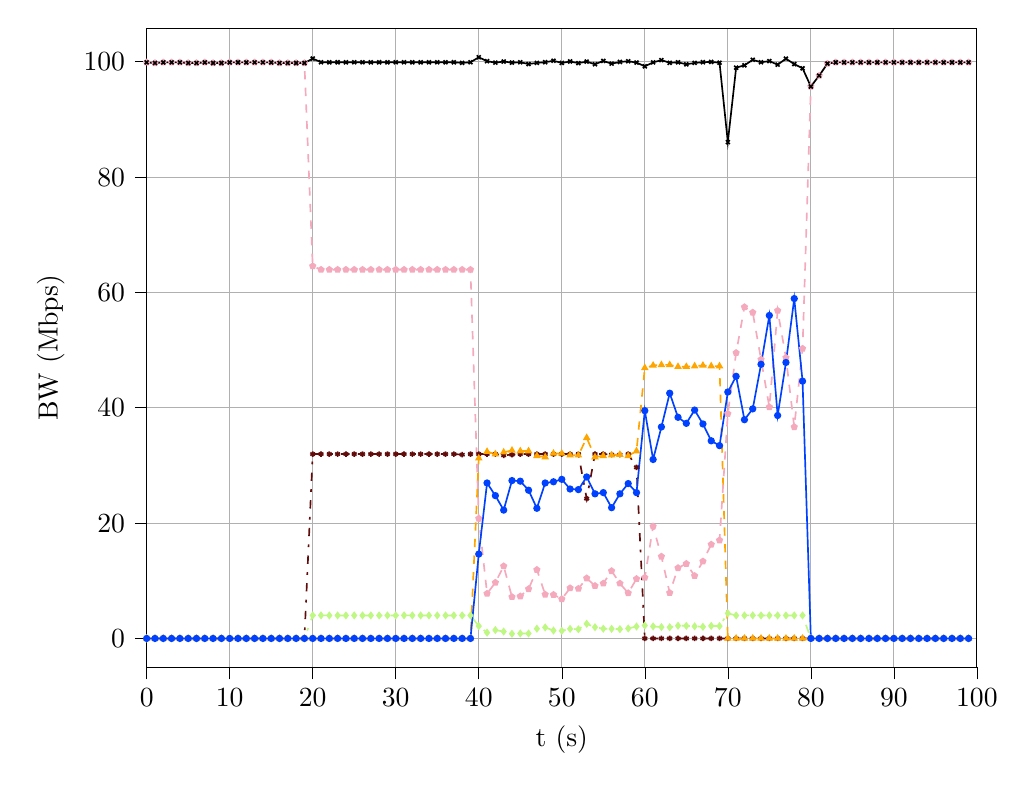
\begin{tikzpicture}

\definecolor{blue064255}{RGB}{0,64,255}
\definecolor{darkgrey176}{RGB}{176,176,176}
\definecolor{lightpink245169188}{RGB}{245,169,188}
\definecolor{maroon971111}{RGB}{97,11,11}
\definecolor{orange}{RGB}{255,165,0}
\definecolor{palegreen190247129}{RGB}{190,247,129}

\begin{axis}[
height=0.8\textwidth,
tick align=outside,
tick pos=left,
width=\textwidth,
x grid style={darkgrey176},
xlabel={t (s)},
xmajorgrids,
xmin=0, xmax=100,
xtick style={color=black},
y grid style={darkgrey176},
ylabel={BW (Mbps)},
ymajorgrids,
ymin=-5.03872622282609, ymax=105.813250679348,
ytick style={color=black}
]
\addplot [semithick, maroon971111, dash pattern=on 1pt off 3pt on 3pt off 3pt, mark=asterisk, mark size=1, mark options={solid}]
table {%
0 0
1 0
2 0
3 0
4 0
5 0
6 0
7 0
8 0
9 0
10 0
11 0
12 0
13 0
14 0
15 0
16 0
17 0
18 0
19 0
20 31.9720108695652
21 31.9720108695652
22 31.9720108695652
23 31.9720108695652
24 31.9720108695652
25 31.9720108695652
26 31.9720108695652
27 31.9720108695652
28 31.9720108695652
29 31.9720108695652
30 31.9720108695652
31 31.9720108695652
32 31.9720108695652
33 31.9720108695652
34 31.9720108695652
35 31.9720108695652
36 31.9720108695652
37 31.9720108695652
38 31.867527173913
39 31.9720108695652
40 31.9720108695652
41 31.9720108695652
42 31.9720108695652
43 31.7630434782609
44 31.867527173913
45 31.9720108695652
46 31.9720108695652
47 31.9720108695652
48 31.9720108695652
49 31.9720108695652
50 31.9720108695652
51 31.9720108695652
52 31.9720108695652
53 24.2402173913043
54 31.9720108695652
55 31.9720108695652
56 31.867527173913
57 31.867527173913
58 31.9720108695652
59 29.6733695652174
60 0
61 0
62 0
63 0
64 0
65 0
66 0
67 0
68 0
69 0
70 0
71 0
72 0
73 0
74 0
75 0
76 0
77 0
78 0
79 0
80 0
81 0
82 0
83 0
84 0
85 0
86 0
87 0
88 0
89 0
90 0
91 0
92 0
93 0
94 0
95 0
96 0
97 0
98 0
99 0
};
\addplot [semithick, palegreen190247129, dash pattern=on 1pt off 3pt on 3pt off 3pt, mark=diamond*, mark size=1, mark options={solid}]
table {%
0 0
1 0
2 0
3 0
4 0
5 0
6 0
7 0
8 0
9 0
10 0
11 0
12 0
13 0
14 0
15 0
16 0
17 0
18 0
19 0
20 4.00172554347826
21 4.00172554347826
22 3.99127717391304
23 3.99127717391304
24 3.99127717391304
25 3.99127717391304
26 3.99127717391304
27 3.99127717391304
28 3.99127717391304
29 3.99127717391304
30 3.99127717391304
31 4.00172554347826
32 3.99127717391304
33 3.99127717391304
34 3.99127717391304
35 3.99127717391304
36 3.99127717391304
37 3.99127717391304
38 3.99127717391304
39 3.99127717391304
40 2.14191576086956
41 1.00722282608696
42 1.45232336956522
43 1.19111413043478
44 0.81079347826087
45 0.859900815217391
46 0.859900815217391
47 1.69263586956522
48 1.91205163043478
49 1.36873641304348
50 1.32694293478261
51 1.66129076086957
52 1.58815217391304
53 2.53895380434783
54 1.94339673913043
55 1.69263586956522
56 1.66129076086957
57 1.60904891304348
58 1.73442934782609
59 2.06877717391304
60 2.24639945652174
61 2.08967391304348
62 1.96429347826087
63 1.94339673913043
64 2.20460597826087
65 2.18370923913043
66 2.1001222826087
67 2.01653532608696
68 2.17326086956522
69 2.14191576086956
70 4.35697010869565
71 3.99127717391304
72 3.99127717391304
73 4.00172554347826
74 3.99127717391304
75 3.99127717391304
76 3.99127717391304
77 3.99127717391304
78 3.99127717391304
79 3.99127717391304
80 0
81 0
82 0
83 0
84 0
85 0
86 0
87 0
88 0
89 0
90 0
91 0
92 0
93 0
94 0
95 0
96 0
97 0
98 0
99 0
};
\addplot [semithick, orange, dashed, mark=triangle*, mark size=1, mark options={solid}]
table {%
0 0
1 0
2 0
3 0
4 0
5 0
6 0
7 0
8 0
9 0
10 0
11 0
12 0
13 0
14 0
15 0
16 0
17 0
18 0
19 0
20 0
21 0
22 0
23 0
24 0
25 0
26 0
27 0
28 0
29 0
30 0
31 0
32 0
33 0
34 0
35 0
36 0
37 0
38 0
39 0
40 31.240625
41 32.3899456521739
42 31.9720108695652
43 32.2854619565217
44 32.5989130434783
45 32.4944293478261
46 32.4944293478261
47 31.6585597826087
48 31.4495923913043
49 32.0764945652174
50 32.0764945652174
51 31.7630434782609
52 31.7630434782609
53 34.7930706521739
54 31.4495923913043
55 31.6585597826087
56 31.7630434782609
57 31.867527173913
58 31.6585597826087
59 32.4944293478261
60 46.9131793478261
61 47.3311141304348
62 47.4355978260869
63 47.4355978260869
64 47.1221467391304
65 47.1221467391304
66 47.2266304347826
67 47.3311141304348
68 47.2266304347826
69 47.2266304347826
70 0
71 0
72 0
73 0
74 0
75 0
76 0
77 0
78 0
79 0
80 0
81 0
82 0
83 0
84 0
85 0
86 0
87 0
88 0
89 0
90 0
91 0
92 0
93 0
94 0
95 0
96 0
97 0
98 0
99 0
};
\addplot [semithick, lightpink245169188, dashed, mark=pentagon*, mark size=1, mark options={solid}]
table {%
0 99.8864130434782
1 99.7819293478261
2 99.8864130434782
3 99.8864130434782
4 99.8864130434782
5 99.7819293478261
6 99.7819293478261
7 99.8864130434782
8 99.7819293478261
9 99.7819293478261
10 99.8864130434782
11 99.8864130434782
12 99.8864130434782
13 99.8864130434782
14 99.8864130434782
15 99.8864130434782
16 99.7819293478261
17 99.7819293478261
18 99.7819293478261
19 99.7819293478261
20 64.5709239130435
21 63.9440217391304
22 63.9440217391304
23 63.9440217391304
24 63.9440217391304
25 63.9440217391304
26 63.9440217391304
27 63.9440217391304
28 63.9440217391304
29 63.9440217391304
30 63.9440217391304
31 63.9440217391304
32 63.9440217391304
33 63.9440217391304
34 63.9440217391304
35 63.9440217391304
36 63.9440217391304
37 63.9440217391304
38 63.9440217391304
39 63.9440217391304
40 20.7922554347826
41 7.77358695652174
42 9.68563858695652
43 12.5380434782609
44 7.19892663043478
45 7.31385869565217
46 8.57811141304348
47 11.9111413043478
48 7.62730978260869
49 7.58551630434783
50 6.83323369565217
51 8.73483695652174
52 8.63035326086956
53 10.4483695652174
54 9.12142663043478
55 9.53936141304348
56 11.7021739130435
57 9.53936141304348
58 7.8676222826087
59 10.3334375
60 10.5528532608696
61 19.4339673913043
62 14.2097826086957
63 7.90941576086956
64 12.2245923913043
65 12.9559782608696
66 10.8663043478261
67 13.3739130434783
68 16.2994565217391
69 17.0308423913043
70 38.9724184782609
71 49.5252717391304
72 57.4660326086956
73 56.5256793478261
74 48.3759510869565
75 40.1217391304348
76 56.8391304347826
77 48.689402173913
78 36.673777173913
79 50.2566576086956
80 95.7070652173913
81 97.5877717391304
82 99.6774456521739
83 99.8864130434782
84 99.8864130434782
85 99.8864130434782
86 99.8864130434782
87 99.8864130434782
88 99.8864130434782
89 99.8864130434782
90 99.8864130434782
91 99.8864130434782
92 99.8864130434782
93 99.8864130434782
94 99.8864130434782
95 99.8864130434782
96 99.8864130434782
97 99.8864130434782
98 99.8864130434782
99 99.8864130434782
};
\addplot [semithick, blue064255, mark=*, mark size=1, mark options={solid}]
table {%
0 0
1 0
2 0
3 0
4 0
5 0
6 0
7 0
8 0
9 0
10 0
11 0
12 0
13 0
14 0
15 0
16 0
17 0
18 0
19 0
20 0
21 0
22 0
23 0
24 0
25 0
26 0
27 0
28 0
29 0
30 0
31 0
32 0
33 0
34 0
35 0
36 0
37 0
38 0
39 0
40 14.6277173913043
41 26.9567934782609
42 24.7626358695652
43 22.255027173913
44 27.3747282608696
45 27.2702445652174
46 25.7029891304348
47 22.5684782608696
48 26.9567934782609
49 27.1657608695652
50 27.5836956521739
51 25.9119565217391
52 25.807472826087
53 28.0016304347826
54 25.0760869565217
55 25.2850543478261
56 22.6729619565217
57 25.0760869565217
58 26.8523097826087
59 25.2850543478261
60 39.4948369565217
61 31.0316576086956
62 36.673777173913
63 42.5248641304348
64 38.3455163043478
65 37.3006793478261
66 39.5993206521739
67 37.1961956521739
68 34.270652173913
69 33.4347826086956
70 42.7338315217391
71 45.4504076086956
72 37.9275815217391
73 39.8082880434783
74 47.5400815217391
75 56.0032608695652
76 38.6589673913043
77 47.8535326086956
78 58.9288043478261
79 44.6145380434783
80 0
81 0
82 0
83 0
84 0
85 0
86 0
87 0
88 0
89 0
90 0
91 0
92 0
93 0
94 0
95 0
96 0
97 0
98 0
99 0
};
\addplot [semithick, black, mark=x, mark size=1, mark options={solid}]
table {%
0 99.8864130434782
1 99.7819293478261
2 99.8864130434782
3 99.8864130434782
4 99.8864130434782
5 99.7819293478261
6 99.7819293478261
7 99.8864130434782
8 99.7819293478261
9 99.7819293478261
10 99.8864130434782
11 99.8864130434782
12 99.8864130434782
13 99.8864130434782
14 99.8864130434782
15 99.8864130434782
16 99.7819293478261
17 99.7819293478261
18 99.7819293478261
19 99.7819293478261
20 100.544660326087
21 99.9177581521739
22 99.9073097826087
23 99.9073097826087
24 99.9073097826087
25 99.9073097826087
26 99.9073097826087
27 99.9073097826087
28 99.9073097826087
29 99.9073097826087
30 99.9073097826087
31 99.9177581521739
32 99.9073097826087
33 99.9073097826087
34 99.9073097826087
35 99.9073097826087
36 99.9073097826087
37 99.9073097826087
38 99.8028260869565
39 99.9073097826087
40 100.774524456522
41 100.099559782609
42 99.8446195652174
43 100.032690217391
44 99.8508885869565
45 99.9104442934782
46 99.607441576087
47 99.8028260869565
48 99.9177581521739
49 100.168519021739
50 99.7923777173913
51 100.043138586957
52 99.7610326086956
53 100.022241847826
54 99.5625135869565
55 100.147622282609
56 99.6669972826087
57 99.9595516304348
58 100.084932065217
59 99.8550679347826
60 99.2072690217391
61 99.8864130434783
62 100.283451086957
63 99.8132744565217
64 99.8968614130435
65 99.5625135869565
66 99.7923777173913
67 99.9177581521739
68 99.97
69 99.8341711956522
70 86.0632201086956
71 98.9669565217391
72 99.3848913043478
73 100.335692934783
74 99.9073097826087
75 100.116277173913
76 99.489375
77 100.534211956522
78 99.5938586956522
79 98.862472826087
80 95.7070652173913
81 97.5877717391304
82 99.6774456521739
83 99.8864130434782
84 99.8864130434782
85 99.8864130434782
86 99.8864130434782
87 99.8864130434782
88 99.8864130434782
89 99.8864130434782
90 99.8864130434782
91 99.8864130434782
92 99.8864130434782
93 99.8864130434782
94 99.8864130434782
95 99.8864130434782
96 99.8864130434782
97 99.8864130434782
98 99.8864130434782
99 99.8864130434782
};
\end{axis}

\end{tikzpicture}

        \hspace*{3.35em}
        \centering \small (a) IETF: Bandwidth Evolution.
    \end{minipage}
    \vspace*{0.25em}
    \hfill
    \begin{minipage}[t]{0.3\textwidth}
        \centering
        % This file was created with tikzplotlib v0.10.1.
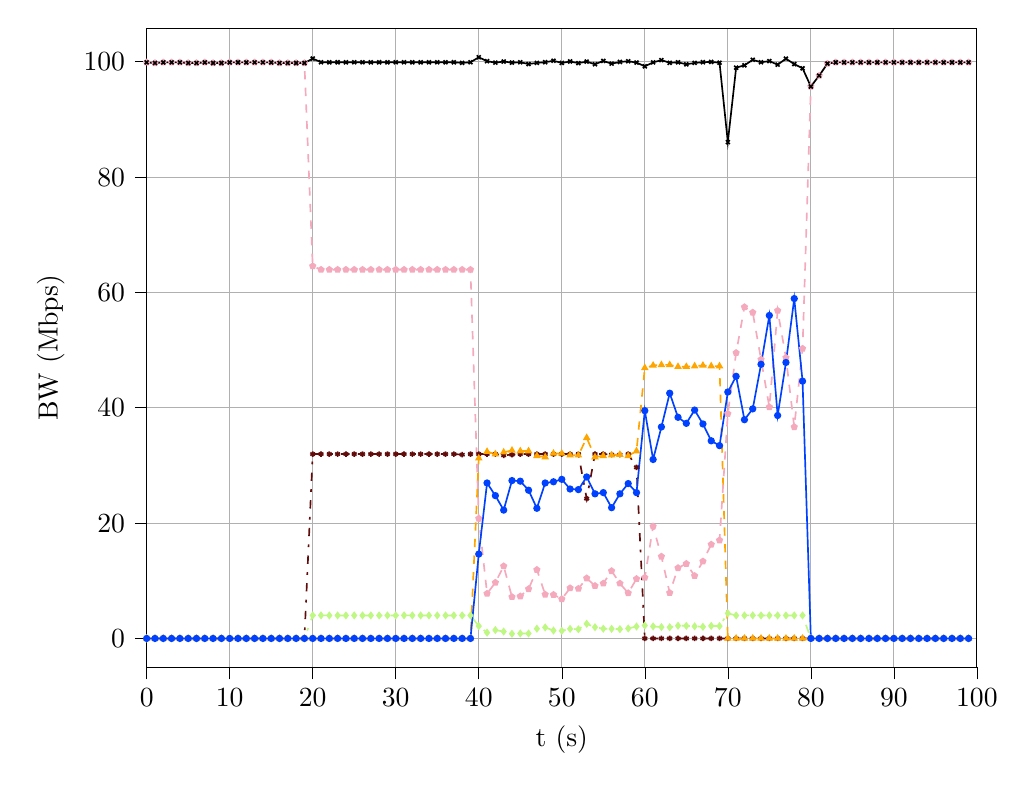
\begin{tikzpicture}

\definecolor{blue064255}{RGB}{0,64,255}
\definecolor{darkgrey176}{RGB}{176,176,176}
\definecolor{lightpink245169188}{RGB}{245,169,188}
\definecolor{maroon971111}{RGB}{97,11,11}
\definecolor{orange}{RGB}{255,165,0}
\definecolor{palegreen190247129}{RGB}{190,247,129}

\begin{axis}[
height=0.8\textwidth,
tick align=outside,
tick pos=left,
width=\textwidth,
x grid style={darkgrey176},
xlabel={t (s)},
xmajorgrids,
xmin=0, xmax=100,
xtick style={color=black},
y grid style={darkgrey176},
ylabel={BW (Mbps)},
ymajorgrids,
ymin=-5.03872622282609, ymax=105.813250679348,
ytick style={color=black}
]
\addplot [semithick, maroon971111, dash pattern=on 1pt off 3pt on 3pt off 3pt, mark=asterisk, mark size=1, mark options={solid}]
table {%
0 0
1 0
2 0
3 0
4 0
5 0
6 0
7 0
8 0
9 0
10 0
11 0
12 0
13 0
14 0
15 0
16 0
17 0
18 0
19 0
20 31.9720108695652
21 31.9720108695652
22 31.9720108695652
23 31.9720108695652
24 31.9720108695652
25 31.9720108695652
26 31.9720108695652
27 31.9720108695652
28 31.9720108695652
29 31.9720108695652
30 31.9720108695652
31 31.9720108695652
32 31.9720108695652
33 31.9720108695652
34 31.9720108695652
35 31.9720108695652
36 31.9720108695652
37 31.9720108695652
38 31.867527173913
39 31.9720108695652
40 31.9720108695652
41 31.9720108695652
42 31.9720108695652
43 31.7630434782609
44 31.867527173913
45 31.9720108695652
46 31.9720108695652
47 31.9720108695652
48 31.9720108695652
49 31.9720108695652
50 31.9720108695652
51 31.9720108695652
52 31.9720108695652
53 24.2402173913043
54 31.9720108695652
55 31.9720108695652
56 31.867527173913
57 31.867527173913
58 31.9720108695652
59 29.6733695652174
60 0
61 0
62 0
63 0
64 0
65 0
66 0
67 0
68 0
69 0
70 0
71 0
72 0
73 0
74 0
75 0
76 0
77 0
78 0
79 0
80 0
81 0
82 0
83 0
84 0
85 0
86 0
87 0
88 0
89 0
90 0
91 0
92 0
93 0
94 0
95 0
96 0
97 0
98 0
99 0
};
\addplot [semithick, palegreen190247129, dash pattern=on 1pt off 3pt on 3pt off 3pt, mark=diamond*, mark size=1, mark options={solid}]
table {%
0 0
1 0
2 0
3 0
4 0
5 0
6 0
7 0
8 0
9 0
10 0
11 0
12 0
13 0
14 0
15 0
16 0
17 0
18 0
19 0
20 4.00172554347826
21 4.00172554347826
22 3.99127717391304
23 3.99127717391304
24 3.99127717391304
25 3.99127717391304
26 3.99127717391304
27 3.99127717391304
28 3.99127717391304
29 3.99127717391304
30 3.99127717391304
31 4.00172554347826
32 3.99127717391304
33 3.99127717391304
34 3.99127717391304
35 3.99127717391304
36 3.99127717391304
37 3.99127717391304
38 3.99127717391304
39 3.99127717391304
40 2.14191576086956
41 1.00722282608696
42 1.45232336956522
43 1.19111413043478
44 0.81079347826087
45 0.859900815217391
46 0.859900815217391
47 1.69263586956522
48 1.91205163043478
49 1.36873641304348
50 1.32694293478261
51 1.66129076086957
52 1.58815217391304
53 2.53895380434783
54 1.94339673913043
55 1.69263586956522
56 1.66129076086957
57 1.60904891304348
58 1.73442934782609
59 2.06877717391304
60 2.24639945652174
61 2.08967391304348
62 1.96429347826087
63 1.94339673913043
64 2.20460597826087
65 2.18370923913043
66 2.1001222826087
67 2.01653532608696
68 2.17326086956522
69 2.14191576086956
70 4.35697010869565
71 3.99127717391304
72 3.99127717391304
73 4.00172554347826
74 3.99127717391304
75 3.99127717391304
76 3.99127717391304
77 3.99127717391304
78 3.99127717391304
79 3.99127717391304
80 0
81 0
82 0
83 0
84 0
85 0
86 0
87 0
88 0
89 0
90 0
91 0
92 0
93 0
94 0
95 0
96 0
97 0
98 0
99 0
};
\addplot [semithick, orange, dashed, mark=triangle*, mark size=1, mark options={solid}]
table {%
0 0
1 0
2 0
3 0
4 0
5 0
6 0
7 0
8 0
9 0
10 0
11 0
12 0
13 0
14 0
15 0
16 0
17 0
18 0
19 0
20 0
21 0
22 0
23 0
24 0
25 0
26 0
27 0
28 0
29 0
30 0
31 0
32 0
33 0
34 0
35 0
36 0
37 0
38 0
39 0
40 31.240625
41 32.3899456521739
42 31.9720108695652
43 32.2854619565217
44 32.5989130434783
45 32.4944293478261
46 32.4944293478261
47 31.6585597826087
48 31.4495923913043
49 32.0764945652174
50 32.0764945652174
51 31.7630434782609
52 31.7630434782609
53 34.7930706521739
54 31.4495923913043
55 31.6585597826087
56 31.7630434782609
57 31.867527173913
58 31.6585597826087
59 32.4944293478261
60 46.9131793478261
61 47.3311141304348
62 47.4355978260869
63 47.4355978260869
64 47.1221467391304
65 47.1221467391304
66 47.2266304347826
67 47.3311141304348
68 47.2266304347826
69 47.2266304347826
70 0
71 0
72 0
73 0
74 0
75 0
76 0
77 0
78 0
79 0
80 0
81 0
82 0
83 0
84 0
85 0
86 0
87 0
88 0
89 0
90 0
91 0
92 0
93 0
94 0
95 0
96 0
97 0
98 0
99 0
};
\addplot [semithick, lightpink245169188, dashed, mark=pentagon*, mark size=1, mark options={solid}]
table {%
0 99.8864130434782
1 99.7819293478261
2 99.8864130434782
3 99.8864130434782
4 99.8864130434782
5 99.7819293478261
6 99.7819293478261
7 99.8864130434782
8 99.7819293478261
9 99.7819293478261
10 99.8864130434782
11 99.8864130434782
12 99.8864130434782
13 99.8864130434782
14 99.8864130434782
15 99.8864130434782
16 99.7819293478261
17 99.7819293478261
18 99.7819293478261
19 99.7819293478261
20 64.5709239130435
21 63.9440217391304
22 63.9440217391304
23 63.9440217391304
24 63.9440217391304
25 63.9440217391304
26 63.9440217391304
27 63.9440217391304
28 63.9440217391304
29 63.9440217391304
30 63.9440217391304
31 63.9440217391304
32 63.9440217391304
33 63.9440217391304
34 63.9440217391304
35 63.9440217391304
36 63.9440217391304
37 63.9440217391304
38 63.9440217391304
39 63.9440217391304
40 20.7922554347826
41 7.77358695652174
42 9.68563858695652
43 12.5380434782609
44 7.19892663043478
45 7.31385869565217
46 8.57811141304348
47 11.9111413043478
48 7.62730978260869
49 7.58551630434783
50 6.83323369565217
51 8.73483695652174
52 8.63035326086956
53 10.4483695652174
54 9.12142663043478
55 9.53936141304348
56 11.7021739130435
57 9.53936141304348
58 7.8676222826087
59 10.3334375
60 10.5528532608696
61 19.4339673913043
62 14.2097826086957
63 7.90941576086956
64 12.2245923913043
65 12.9559782608696
66 10.8663043478261
67 13.3739130434783
68 16.2994565217391
69 17.0308423913043
70 38.9724184782609
71 49.5252717391304
72 57.4660326086956
73 56.5256793478261
74 48.3759510869565
75 40.1217391304348
76 56.8391304347826
77 48.689402173913
78 36.673777173913
79 50.2566576086956
80 95.7070652173913
81 97.5877717391304
82 99.6774456521739
83 99.8864130434782
84 99.8864130434782
85 99.8864130434782
86 99.8864130434782
87 99.8864130434782
88 99.8864130434782
89 99.8864130434782
90 99.8864130434782
91 99.8864130434782
92 99.8864130434782
93 99.8864130434782
94 99.8864130434782
95 99.8864130434782
96 99.8864130434782
97 99.8864130434782
98 99.8864130434782
99 99.8864130434782
};
\addplot [semithick, blue064255, mark=*, mark size=1, mark options={solid}]
table {%
0 0
1 0
2 0
3 0
4 0
5 0
6 0
7 0
8 0
9 0
10 0
11 0
12 0
13 0
14 0
15 0
16 0
17 0
18 0
19 0
20 0
21 0
22 0
23 0
24 0
25 0
26 0
27 0
28 0
29 0
30 0
31 0
32 0
33 0
34 0
35 0
36 0
37 0
38 0
39 0
40 14.6277173913043
41 26.9567934782609
42 24.7626358695652
43 22.255027173913
44 27.3747282608696
45 27.2702445652174
46 25.7029891304348
47 22.5684782608696
48 26.9567934782609
49 27.1657608695652
50 27.5836956521739
51 25.9119565217391
52 25.807472826087
53 28.0016304347826
54 25.0760869565217
55 25.2850543478261
56 22.6729619565217
57 25.0760869565217
58 26.8523097826087
59 25.2850543478261
60 39.4948369565217
61 31.0316576086956
62 36.673777173913
63 42.5248641304348
64 38.3455163043478
65 37.3006793478261
66 39.5993206521739
67 37.1961956521739
68 34.270652173913
69 33.4347826086956
70 42.7338315217391
71 45.4504076086956
72 37.9275815217391
73 39.8082880434783
74 47.5400815217391
75 56.0032608695652
76 38.6589673913043
77 47.8535326086956
78 58.9288043478261
79 44.6145380434783
80 0
81 0
82 0
83 0
84 0
85 0
86 0
87 0
88 0
89 0
90 0
91 0
92 0
93 0
94 0
95 0
96 0
97 0
98 0
99 0
};
\addplot [semithick, black, mark=x, mark size=1, mark options={solid}]
table {%
0 99.8864130434782
1 99.7819293478261
2 99.8864130434782
3 99.8864130434782
4 99.8864130434782
5 99.7819293478261
6 99.7819293478261
7 99.8864130434782
8 99.7819293478261
9 99.7819293478261
10 99.8864130434782
11 99.8864130434782
12 99.8864130434782
13 99.8864130434782
14 99.8864130434782
15 99.8864130434782
16 99.7819293478261
17 99.7819293478261
18 99.7819293478261
19 99.7819293478261
20 100.544660326087
21 99.9177581521739
22 99.9073097826087
23 99.9073097826087
24 99.9073097826087
25 99.9073097826087
26 99.9073097826087
27 99.9073097826087
28 99.9073097826087
29 99.9073097826087
30 99.9073097826087
31 99.9177581521739
32 99.9073097826087
33 99.9073097826087
34 99.9073097826087
35 99.9073097826087
36 99.9073097826087
37 99.9073097826087
38 99.8028260869565
39 99.9073097826087
40 100.774524456522
41 100.099559782609
42 99.8446195652174
43 100.032690217391
44 99.8508885869565
45 99.9104442934782
46 99.607441576087
47 99.8028260869565
48 99.9177581521739
49 100.168519021739
50 99.7923777173913
51 100.043138586957
52 99.7610326086956
53 100.022241847826
54 99.5625135869565
55 100.147622282609
56 99.6669972826087
57 99.9595516304348
58 100.084932065217
59 99.8550679347826
60 99.2072690217391
61 99.8864130434783
62 100.283451086957
63 99.8132744565217
64 99.8968614130435
65 99.5625135869565
66 99.7923777173913
67 99.9177581521739
68 99.97
69 99.8341711956522
70 86.0632201086956
71 98.9669565217391
72 99.3848913043478
73 100.335692934783
74 99.9073097826087
75 100.116277173913
76 99.489375
77 100.534211956522
78 99.5938586956522
79 98.862472826087
80 95.7070652173913
81 97.5877717391304
82 99.6774456521739
83 99.8864130434782
84 99.8864130434782
85 99.8864130434782
86 99.8864130434782
87 99.8864130434782
88 99.8864130434782
89 99.8864130434782
90 99.8864130434782
91 99.8864130434782
92 99.8864130434782
93 99.8864130434782
94 99.8864130434782
95 99.8864130434782
96 99.8864130434782
97 99.8864130434782
98 99.8864130434782
99 99.8864130434782
};
\end{axis}

\end{tikzpicture}

        \hspace*{3.5em}
        \centering \small (b) \cite{Lin2021}: Bandwidth Evolution.
    \end{minipage}
    \vspace*{0.25em}
    \hfill
    \begin{minipage}[t]{0.3\textwidth}
        \centering
        % This file was created with tikzplotlib v0.10.1.
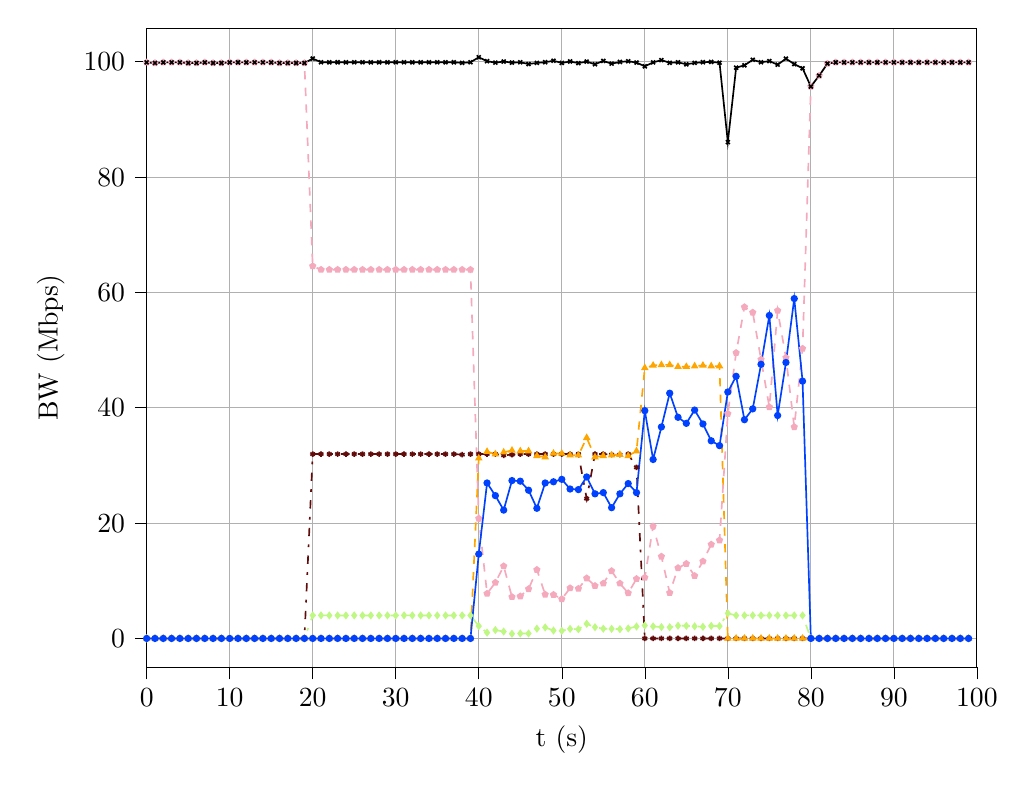
\begin{tikzpicture}

\definecolor{blue064255}{RGB}{0,64,255}
\definecolor{darkgrey176}{RGB}{176,176,176}
\definecolor{lightpink245169188}{RGB}{245,169,188}
\definecolor{maroon971111}{RGB}{97,11,11}
\definecolor{orange}{RGB}{255,165,0}
\definecolor{palegreen190247129}{RGB}{190,247,129}

\begin{axis}[
height=0.8\textwidth,
tick align=outside,
tick pos=left,
width=\textwidth,
x grid style={darkgrey176},
xlabel={t (s)},
xmajorgrids,
xmin=0, xmax=100,
xtick style={color=black},
y grid style={darkgrey176},
ylabel={BW (Mbps)},
ymajorgrids,
ymin=-5.03872622282609, ymax=105.813250679348,
ytick style={color=black}
]
\addplot [semithick, maroon971111, dash pattern=on 1pt off 3pt on 3pt off 3pt, mark=asterisk, mark size=1, mark options={solid}]
table {%
0 0
1 0
2 0
3 0
4 0
5 0
6 0
7 0
8 0
9 0
10 0
11 0
12 0
13 0
14 0
15 0
16 0
17 0
18 0
19 0
20 31.9720108695652
21 31.9720108695652
22 31.9720108695652
23 31.9720108695652
24 31.9720108695652
25 31.9720108695652
26 31.9720108695652
27 31.9720108695652
28 31.9720108695652
29 31.9720108695652
30 31.9720108695652
31 31.9720108695652
32 31.9720108695652
33 31.9720108695652
34 31.9720108695652
35 31.9720108695652
36 31.9720108695652
37 31.9720108695652
38 31.867527173913
39 31.9720108695652
40 31.9720108695652
41 31.9720108695652
42 31.9720108695652
43 31.7630434782609
44 31.867527173913
45 31.9720108695652
46 31.9720108695652
47 31.9720108695652
48 31.9720108695652
49 31.9720108695652
50 31.9720108695652
51 31.9720108695652
52 31.9720108695652
53 24.2402173913043
54 31.9720108695652
55 31.9720108695652
56 31.867527173913
57 31.867527173913
58 31.9720108695652
59 29.6733695652174
60 0
61 0
62 0
63 0
64 0
65 0
66 0
67 0
68 0
69 0
70 0
71 0
72 0
73 0
74 0
75 0
76 0
77 0
78 0
79 0
80 0
81 0
82 0
83 0
84 0
85 0
86 0
87 0
88 0
89 0
90 0
91 0
92 0
93 0
94 0
95 0
96 0
97 0
98 0
99 0
};
\addplot [semithick, palegreen190247129, dash pattern=on 1pt off 3pt on 3pt off 3pt, mark=diamond*, mark size=1, mark options={solid}]
table {%
0 0
1 0
2 0
3 0
4 0
5 0
6 0
7 0
8 0
9 0
10 0
11 0
12 0
13 0
14 0
15 0
16 0
17 0
18 0
19 0
20 4.00172554347826
21 4.00172554347826
22 3.99127717391304
23 3.99127717391304
24 3.99127717391304
25 3.99127717391304
26 3.99127717391304
27 3.99127717391304
28 3.99127717391304
29 3.99127717391304
30 3.99127717391304
31 4.00172554347826
32 3.99127717391304
33 3.99127717391304
34 3.99127717391304
35 3.99127717391304
36 3.99127717391304
37 3.99127717391304
38 3.99127717391304
39 3.99127717391304
40 2.14191576086956
41 1.00722282608696
42 1.45232336956522
43 1.19111413043478
44 0.81079347826087
45 0.859900815217391
46 0.859900815217391
47 1.69263586956522
48 1.91205163043478
49 1.36873641304348
50 1.32694293478261
51 1.66129076086957
52 1.58815217391304
53 2.53895380434783
54 1.94339673913043
55 1.69263586956522
56 1.66129076086957
57 1.60904891304348
58 1.73442934782609
59 2.06877717391304
60 2.24639945652174
61 2.08967391304348
62 1.96429347826087
63 1.94339673913043
64 2.20460597826087
65 2.18370923913043
66 2.1001222826087
67 2.01653532608696
68 2.17326086956522
69 2.14191576086956
70 4.35697010869565
71 3.99127717391304
72 3.99127717391304
73 4.00172554347826
74 3.99127717391304
75 3.99127717391304
76 3.99127717391304
77 3.99127717391304
78 3.99127717391304
79 3.99127717391304
80 0
81 0
82 0
83 0
84 0
85 0
86 0
87 0
88 0
89 0
90 0
91 0
92 0
93 0
94 0
95 0
96 0
97 0
98 0
99 0
};
\addplot [semithick, orange, dashed, mark=triangle*, mark size=1, mark options={solid}]
table {%
0 0
1 0
2 0
3 0
4 0
5 0
6 0
7 0
8 0
9 0
10 0
11 0
12 0
13 0
14 0
15 0
16 0
17 0
18 0
19 0
20 0
21 0
22 0
23 0
24 0
25 0
26 0
27 0
28 0
29 0
30 0
31 0
32 0
33 0
34 0
35 0
36 0
37 0
38 0
39 0
40 31.240625
41 32.3899456521739
42 31.9720108695652
43 32.2854619565217
44 32.5989130434783
45 32.4944293478261
46 32.4944293478261
47 31.6585597826087
48 31.4495923913043
49 32.0764945652174
50 32.0764945652174
51 31.7630434782609
52 31.7630434782609
53 34.7930706521739
54 31.4495923913043
55 31.6585597826087
56 31.7630434782609
57 31.867527173913
58 31.6585597826087
59 32.4944293478261
60 46.9131793478261
61 47.3311141304348
62 47.4355978260869
63 47.4355978260869
64 47.1221467391304
65 47.1221467391304
66 47.2266304347826
67 47.3311141304348
68 47.2266304347826
69 47.2266304347826
70 0
71 0
72 0
73 0
74 0
75 0
76 0
77 0
78 0
79 0
80 0
81 0
82 0
83 0
84 0
85 0
86 0
87 0
88 0
89 0
90 0
91 0
92 0
93 0
94 0
95 0
96 0
97 0
98 0
99 0
};
\addplot [semithick, lightpink245169188, dashed, mark=pentagon*, mark size=1, mark options={solid}]
table {%
0 99.8864130434782
1 99.7819293478261
2 99.8864130434782
3 99.8864130434782
4 99.8864130434782
5 99.7819293478261
6 99.7819293478261
7 99.8864130434782
8 99.7819293478261
9 99.7819293478261
10 99.8864130434782
11 99.8864130434782
12 99.8864130434782
13 99.8864130434782
14 99.8864130434782
15 99.8864130434782
16 99.7819293478261
17 99.7819293478261
18 99.7819293478261
19 99.7819293478261
20 64.5709239130435
21 63.9440217391304
22 63.9440217391304
23 63.9440217391304
24 63.9440217391304
25 63.9440217391304
26 63.9440217391304
27 63.9440217391304
28 63.9440217391304
29 63.9440217391304
30 63.9440217391304
31 63.9440217391304
32 63.9440217391304
33 63.9440217391304
34 63.9440217391304
35 63.9440217391304
36 63.9440217391304
37 63.9440217391304
38 63.9440217391304
39 63.9440217391304
40 20.7922554347826
41 7.77358695652174
42 9.68563858695652
43 12.5380434782609
44 7.19892663043478
45 7.31385869565217
46 8.57811141304348
47 11.9111413043478
48 7.62730978260869
49 7.58551630434783
50 6.83323369565217
51 8.73483695652174
52 8.63035326086956
53 10.4483695652174
54 9.12142663043478
55 9.53936141304348
56 11.7021739130435
57 9.53936141304348
58 7.8676222826087
59 10.3334375
60 10.5528532608696
61 19.4339673913043
62 14.2097826086957
63 7.90941576086956
64 12.2245923913043
65 12.9559782608696
66 10.8663043478261
67 13.3739130434783
68 16.2994565217391
69 17.0308423913043
70 38.9724184782609
71 49.5252717391304
72 57.4660326086956
73 56.5256793478261
74 48.3759510869565
75 40.1217391304348
76 56.8391304347826
77 48.689402173913
78 36.673777173913
79 50.2566576086956
80 95.7070652173913
81 97.5877717391304
82 99.6774456521739
83 99.8864130434782
84 99.8864130434782
85 99.8864130434782
86 99.8864130434782
87 99.8864130434782
88 99.8864130434782
89 99.8864130434782
90 99.8864130434782
91 99.8864130434782
92 99.8864130434782
93 99.8864130434782
94 99.8864130434782
95 99.8864130434782
96 99.8864130434782
97 99.8864130434782
98 99.8864130434782
99 99.8864130434782
};
\addplot [semithick, blue064255, mark=*, mark size=1, mark options={solid}]
table {%
0 0
1 0
2 0
3 0
4 0
5 0
6 0
7 0
8 0
9 0
10 0
11 0
12 0
13 0
14 0
15 0
16 0
17 0
18 0
19 0
20 0
21 0
22 0
23 0
24 0
25 0
26 0
27 0
28 0
29 0
30 0
31 0
32 0
33 0
34 0
35 0
36 0
37 0
38 0
39 0
40 14.6277173913043
41 26.9567934782609
42 24.7626358695652
43 22.255027173913
44 27.3747282608696
45 27.2702445652174
46 25.7029891304348
47 22.5684782608696
48 26.9567934782609
49 27.1657608695652
50 27.5836956521739
51 25.9119565217391
52 25.807472826087
53 28.0016304347826
54 25.0760869565217
55 25.2850543478261
56 22.6729619565217
57 25.0760869565217
58 26.8523097826087
59 25.2850543478261
60 39.4948369565217
61 31.0316576086956
62 36.673777173913
63 42.5248641304348
64 38.3455163043478
65 37.3006793478261
66 39.5993206521739
67 37.1961956521739
68 34.270652173913
69 33.4347826086956
70 42.7338315217391
71 45.4504076086956
72 37.9275815217391
73 39.8082880434783
74 47.5400815217391
75 56.0032608695652
76 38.6589673913043
77 47.8535326086956
78 58.9288043478261
79 44.6145380434783
80 0
81 0
82 0
83 0
84 0
85 0
86 0
87 0
88 0
89 0
90 0
91 0
92 0
93 0
94 0
95 0
96 0
97 0
98 0
99 0
};
\addplot [semithick, black, mark=x, mark size=1, mark options={solid}]
table {%
0 99.8864130434782
1 99.7819293478261
2 99.8864130434782
3 99.8864130434782
4 99.8864130434782
5 99.7819293478261
6 99.7819293478261
7 99.8864130434782
8 99.7819293478261
9 99.7819293478261
10 99.8864130434782
11 99.8864130434782
12 99.8864130434782
13 99.8864130434782
14 99.8864130434782
15 99.8864130434782
16 99.7819293478261
17 99.7819293478261
18 99.7819293478261
19 99.7819293478261
20 100.544660326087
21 99.9177581521739
22 99.9073097826087
23 99.9073097826087
24 99.9073097826087
25 99.9073097826087
26 99.9073097826087
27 99.9073097826087
28 99.9073097826087
29 99.9073097826087
30 99.9073097826087
31 99.9177581521739
32 99.9073097826087
33 99.9073097826087
34 99.9073097826087
35 99.9073097826087
36 99.9073097826087
37 99.9073097826087
38 99.8028260869565
39 99.9073097826087
40 100.774524456522
41 100.099559782609
42 99.8446195652174
43 100.032690217391
44 99.8508885869565
45 99.9104442934782
46 99.607441576087
47 99.8028260869565
48 99.9177581521739
49 100.168519021739
50 99.7923777173913
51 100.043138586957
52 99.7610326086956
53 100.022241847826
54 99.5625135869565
55 100.147622282609
56 99.6669972826087
57 99.9595516304348
58 100.084932065217
59 99.8550679347826
60 99.2072690217391
61 99.8864130434783
62 100.283451086957
63 99.8132744565217
64 99.8968614130435
65 99.5625135869565
66 99.7923777173913
67 99.9177581521739
68 99.97
69 99.8341711956522
70 86.0632201086956
71 98.9669565217391
72 99.3848913043478
73 100.335692934783
74 99.9073097826087
75 100.116277173913
76 99.489375
77 100.534211956522
78 99.5938586956522
79 98.862472826087
80 95.7070652173913
81 97.5877717391304
82 99.6774456521739
83 99.8864130434782
84 99.8864130434782
85 99.8864130434782
86 99.8864130434782
87 99.8864130434782
88 99.8864130434782
89 99.8864130434782
90 99.8864130434782
91 99.8864130434782
92 99.8864130434782
93 99.8864130434782
94 99.8864130434782
95 99.8864130434782
96 99.8864130434782
97 99.8864130434782
98 99.8864130434782
99 99.8864130434782
};
\end{axis}

\end{tikzpicture}

        \hspace*{3.35em}
        \centering \small (c) \gls{hctns}: Bandwidth Evolution.
    \end{minipage}
    \vspace*{0.25em}

    % SEGUNDA FILA
    \begin{minipage}[t]{0.3\textwidth}
        \centering
        % This file was created with tikzplotlib v0.10.1.
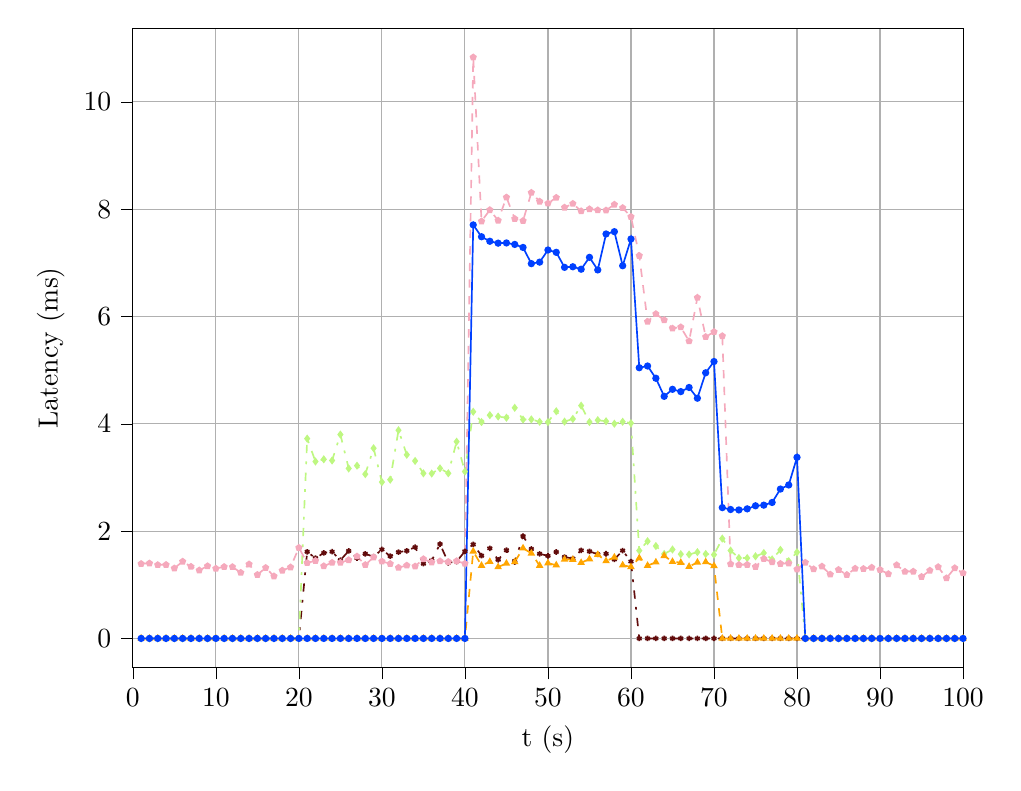
\begin{tikzpicture}

\definecolor{blue064255}{RGB}{0,64,255}
\definecolor{darkgrey176}{RGB}{176,176,176}
\definecolor{lightpink245169188}{RGB}{245,169,188}
\definecolor{maroon971111}{RGB}{97,11,11}
\definecolor{orange}{RGB}{255,165,0}
\definecolor{palegreen190247129}{RGB}{190,247,129}

\begin{axis}[
height=0.8\textwidth,
tick align=outside,
tick pos=left,
width=\textwidth,
x grid style={darkgrey176},
xlabel={t (s)},
xmajorgrids,
xmin=0, xmax=100,
xtick style={color=black},
y grid style={darkgrey176},
ylabel={Latency (ms)},
ymajorgrids,
ymin=-0.54155, ymax=11.37255,
ytick style={color=black}
]
\addplot [semithick, maroon971111, dash pattern=on 1pt off 3pt on 3pt off 3pt, mark=asterisk, mark size=1, mark options={solid}]
table {%
1 0
2 0
3 0
4 0
5 0
6 0
7 0
8 0
9 0
10 0
11 0
12 0
13 0
14 0
15 0
16 0
17 0
18 0
19 0
20 0
21 1.615
22 1.496
23 1.593
24 1.616
25 1.459
26 1.63
27 1.497
28 1.577
29 1.523
30 1.658
31 1.533
32 1.608
33 1.633
34 1.701
35 1.393
36 1.451
37 1.759
38 1.41
39 1.433
40 1.624
41 1.752
42 1.542
43 1.68
44 1.465
45 1.644
46 1.422
47 1.907
48 1.667
49 1.577
50 1.539
51 1.611
52 1.517
53 1.488
54 1.643
55 1.623
56 1.568
57 1.578
58 1.473
59 1.637
60 1.433
61 0
62 0
63 0
64 0
65 0
66 0
67 0
68 0
69 0
70 0
71 0
72 0
73 0
74 0
75 0
76 0
77 0
78 0
79 0
80 0
81 0
82 0
83 0
84 0
85 0
86 0
87 0
88 0
89 0
90 0
91 0
92 0
93 0
94 0
95 0
96 0
97 0
98 0
99 0
100 0
};
\addplot [semithick, palegreen190247129, dash pattern=on 1pt off 3pt on 3pt off 3pt, mark=diamond*, mark size=1, mark options={solid}]
table {%
1 0
2 0
3 0
4 0
5 0
6 0
7 0
8 0
9 0
10 0
11 0
12 0
13 0
14 0
15 0
16 0
17 0
18 0
19 0
20 0
21 3.724
22 3.297
23 3.338
24 3.316
25 3.8
26 3.168
27 3.22
28 3.062
29 3.545
30 2.914
31 2.959
32 3.88
33 3.423
34 3.308
35 3.077
36 3.073
37 3.17
38 3.078
39 3.667
40 3.11
41 4.225
42 4.032
43 4.161
44 4.136
45 4.114
46 4.298
47 4.079
48 4.082
49 4.038
50 4.032
51 4.234
52 4.041
53 4.091
54 4.339
55 4.033
56 4.068
57 4.047
58 4.002
59 4.038
60 4.012
61 1.637
62 1.812
63 1.722
64 1.575
65 1.657
66 1.571
67 1.565
68 1.608
69 1.574
70 1.561
71 1.861
72 1.638
73 1.499
74 1.498
75 1.531
76 1.592
77 1.474
78 1.651
79 1.44
80 1.607
81 0
82 0
83 0
84 0
85 0
86 0
87 0
88 0
89 0
90 0
91 0
92 0
93 0
94 0
95 0
96 0
97 0
98 0
99 0
100 0
};
\addplot [semithick, orange, dashed, mark=triangle*, mark size=1, mark options={solid}]
table {%
1 0
2 0
3 0
4 0
5 0
6 0
7 0
8 0
9 0
10 0
11 0
12 0
13 0
14 0
15 0
16 0
17 0
18 0
19 0
20 0
21 0
22 0
23 0
24 0
25 0
26 0
27 0
28 0
29 0
30 0
31 0
32 0
33 0
34 0
35 0
36 0
37 0
38 0
39 0
40 0
41 1.624
42 1.358
43 1.429
44 1.331
45 1.398
46 1.424
47 1.682
48 1.586
49 1.357
50 1.403
51 1.366
52 1.473
53 1.468
54 1.411
55 1.479
56 1.56
57 1.443
58 1.512
59 1.365
60 1.333
61 1.497
62 1.357
63 1.42
64 1.54
65 1.43
66 1.413
67 1.338
68 1.417
69 1.424
70 1.352
71 0
72 0
73 0
74 0
75 0
76 0
77 0
78 0
79 0
80 0
81 0
82 0
83 0
84 0
85 0
86 0
87 0
88 0
89 0
90 0
91 0
92 0
93 0
94 0
95 0
96 0
97 0
98 0
99 0
100 0
};
\addplot [semithick, lightpink245169188, dashed, mark=pentagon*, mark size=1, mark options={solid}]
table {%
1 1.391
2 1.4
3 1.37
4 1.373
5 1.308
6 1.434
7 1.338
8 1.27
9 1.349
10 1.303
11 1.335
12 1.333
13 1.226
14 1.383
15 1.187
16 1.317
17 1.16
18 1.267
19 1.327
20 1.691
21 1.408
22 1.448
23 1.349
24 1.413
25 1.412
26 1.462
27 1.53
28 1.371
29 1.513
30 1.436
31 1.392
32 1.32
33 1.361
34 1.344
35 1.48
36 1.42
37 1.44
38 1.429
39 1.443
40 1.395
41 10.831
42 7.775
43 7.986
44 7.79
45 8.221
46 7.821
47 7.784
48 8.308
49 8.144
50 8.108
51 8.215
52 8.032
53 8.103
54 7.964
55 8.002
56 7.982
57 7.979
58 8.087
59 8.025
60 7.859
61 7.133
62 5.905
63 6.048
64 5.934
65 5.778
66 5.802
67 5.54
68 6.352
69 5.621
70 5.714
71 5.637
72 1.386
73 1.371
74 1.374
75 1.336
76 1.484
77 1.425
78 1.393
79 1.399
80 1.289
81 1.415
82 1.292
83 1.343
84 1.193
85 1.281
86 1.186
87 1.303
88 1.298
89 1.322
90 1.28
91 1.202
92 1.368
93 1.245
94 1.248
95 1.15
96 1.267
97 1.332
98 1.124
99 1.312
100 1.217
};
\addplot [semithick, blue064255, mark=*, mark size=1, mark options={solid}]
table {%
1 0
2 0
3 0
4 0
5 0
6 0
7 0
8 0
9 0
10 0
11 0
12 0
13 0
14 0
15 0
16 0
17 0
18 0
19 0
20 0
21 0
22 0
23 0
24 0
25 0
26 0
27 0
28 0
29 0
30 0
31 0
32 0
33 0
34 0
35 0
36 0
37 0
38 0
39 0
40 0
41 7.707
42 7.486
43 7.402
44 7.367
45 7.371
46 7.343
47 7.287
48 6.985
49 7.013
50 7.239
51 7.196
52 6.916
53 6.927
54 6.881
55 7.102
56 6.868
57 7.538
58 7.581
59 6.946
60 7.444
61 5.045
62 5.077
63 4.849
64 4.512
65 4.643
66 4.6
67 4.677
68 4.477
69 4.951
70 5.161
71 2.438
72 2.403
73 2.395
74 2.415
75 2.472
76 2.484
77 2.534
78 2.784
79 2.86
80 3.375
81 0
82 0
83 0
84 0
85 0
86 0
87 0
88 0
89 0
90 0
91 0
92 0
93 0
94 0
95 0
96 0
97 0
98 0
99 0
100 0
};
\end{axis}

\end{tikzpicture}

        \hspace*{3.35em}
        \centering \small (d) IETF: Latency Evolution.
    \end{minipage}
    \vspace*{0.25em}
    \hfill
    \begin{minipage}[t]{0.3\textwidth}
        \centering
        % This file was created with tikzplotlib v0.10.1.
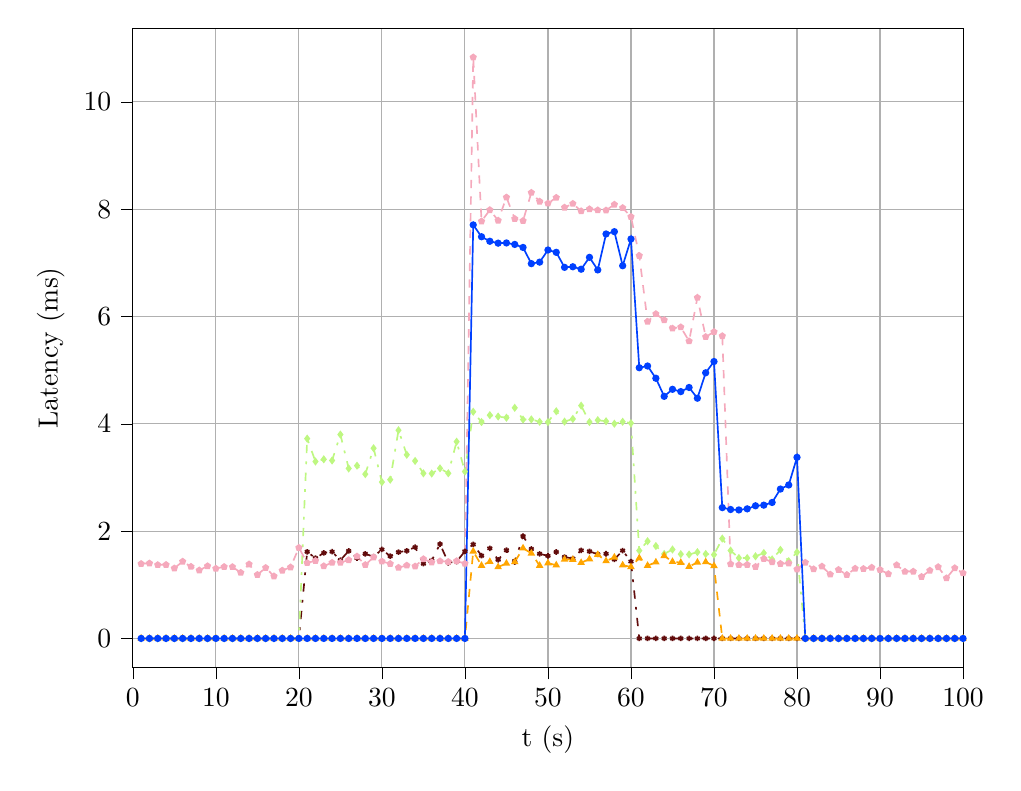
\begin{tikzpicture}

\definecolor{blue064255}{RGB}{0,64,255}
\definecolor{darkgrey176}{RGB}{176,176,176}
\definecolor{lightpink245169188}{RGB}{245,169,188}
\definecolor{maroon971111}{RGB}{97,11,11}
\definecolor{orange}{RGB}{255,165,0}
\definecolor{palegreen190247129}{RGB}{190,247,129}

\begin{axis}[
height=0.8\textwidth,
tick align=outside,
tick pos=left,
width=\textwidth,
x grid style={darkgrey176},
xlabel={t (s)},
xmajorgrids,
xmin=0, xmax=100,
xtick style={color=black},
y grid style={darkgrey176},
ylabel={Latency (ms)},
ymajorgrids,
ymin=-0.54155, ymax=11.37255,
ytick style={color=black}
]
\addplot [semithick, maroon971111, dash pattern=on 1pt off 3pt on 3pt off 3pt, mark=asterisk, mark size=1, mark options={solid}]
table {%
1 0
2 0
3 0
4 0
5 0
6 0
7 0
8 0
9 0
10 0
11 0
12 0
13 0
14 0
15 0
16 0
17 0
18 0
19 0
20 0
21 1.615
22 1.496
23 1.593
24 1.616
25 1.459
26 1.63
27 1.497
28 1.577
29 1.523
30 1.658
31 1.533
32 1.608
33 1.633
34 1.701
35 1.393
36 1.451
37 1.759
38 1.41
39 1.433
40 1.624
41 1.752
42 1.542
43 1.68
44 1.465
45 1.644
46 1.422
47 1.907
48 1.667
49 1.577
50 1.539
51 1.611
52 1.517
53 1.488
54 1.643
55 1.623
56 1.568
57 1.578
58 1.473
59 1.637
60 1.433
61 0
62 0
63 0
64 0
65 0
66 0
67 0
68 0
69 0
70 0
71 0
72 0
73 0
74 0
75 0
76 0
77 0
78 0
79 0
80 0
81 0
82 0
83 0
84 0
85 0
86 0
87 0
88 0
89 0
90 0
91 0
92 0
93 0
94 0
95 0
96 0
97 0
98 0
99 0
100 0
};
\addplot [semithick, palegreen190247129, dash pattern=on 1pt off 3pt on 3pt off 3pt, mark=diamond*, mark size=1, mark options={solid}]
table {%
1 0
2 0
3 0
4 0
5 0
6 0
7 0
8 0
9 0
10 0
11 0
12 0
13 0
14 0
15 0
16 0
17 0
18 0
19 0
20 0
21 3.724
22 3.297
23 3.338
24 3.316
25 3.8
26 3.168
27 3.22
28 3.062
29 3.545
30 2.914
31 2.959
32 3.88
33 3.423
34 3.308
35 3.077
36 3.073
37 3.17
38 3.078
39 3.667
40 3.11
41 4.225
42 4.032
43 4.161
44 4.136
45 4.114
46 4.298
47 4.079
48 4.082
49 4.038
50 4.032
51 4.234
52 4.041
53 4.091
54 4.339
55 4.033
56 4.068
57 4.047
58 4.002
59 4.038
60 4.012
61 1.637
62 1.812
63 1.722
64 1.575
65 1.657
66 1.571
67 1.565
68 1.608
69 1.574
70 1.561
71 1.861
72 1.638
73 1.499
74 1.498
75 1.531
76 1.592
77 1.474
78 1.651
79 1.44
80 1.607
81 0
82 0
83 0
84 0
85 0
86 0
87 0
88 0
89 0
90 0
91 0
92 0
93 0
94 0
95 0
96 0
97 0
98 0
99 0
100 0
};
\addplot [semithick, orange, dashed, mark=triangle*, mark size=1, mark options={solid}]
table {%
1 0
2 0
3 0
4 0
5 0
6 0
7 0
8 0
9 0
10 0
11 0
12 0
13 0
14 0
15 0
16 0
17 0
18 0
19 0
20 0
21 0
22 0
23 0
24 0
25 0
26 0
27 0
28 0
29 0
30 0
31 0
32 0
33 0
34 0
35 0
36 0
37 0
38 0
39 0
40 0
41 1.624
42 1.358
43 1.429
44 1.331
45 1.398
46 1.424
47 1.682
48 1.586
49 1.357
50 1.403
51 1.366
52 1.473
53 1.468
54 1.411
55 1.479
56 1.56
57 1.443
58 1.512
59 1.365
60 1.333
61 1.497
62 1.357
63 1.42
64 1.54
65 1.43
66 1.413
67 1.338
68 1.417
69 1.424
70 1.352
71 0
72 0
73 0
74 0
75 0
76 0
77 0
78 0
79 0
80 0
81 0
82 0
83 0
84 0
85 0
86 0
87 0
88 0
89 0
90 0
91 0
92 0
93 0
94 0
95 0
96 0
97 0
98 0
99 0
100 0
};
\addplot [semithick, lightpink245169188, dashed, mark=pentagon*, mark size=1, mark options={solid}]
table {%
1 1.391
2 1.4
3 1.37
4 1.373
5 1.308
6 1.434
7 1.338
8 1.27
9 1.349
10 1.303
11 1.335
12 1.333
13 1.226
14 1.383
15 1.187
16 1.317
17 1.16
18 1.267
19 1.327
20 1.691
21 1.408
22 1.448
23 1.349
24 1.413
25 1.412
26 1.462
27 1.53
28 1.371
29 1.513
30 1.436
31 1.392
32 1.32
33 1.361
34 1.344
35 1.48
36 1.42
37 1.44
38 1.429
39 1.443
40 1.395
41 10.831
42 7.775
43 7.986
44 7.79
45 8.221
46 7.821
47 7.784
48 8.308
49 8.144
50 8.108
51 8.215
52 8.032
53 8.103
54 7.964
55 8.002
56 7.982
57 7.979
58 8.087
59 8.025
60 7.859
61 7.133
62 5.905
63 6.048
64 5.934
65 5.778
66 5.802
67 5.54
68 6.352
69 5.621
70 5.714
71 5.637
72 1.386
73 1.371
74 1.374
75 1.336
76 1.484
77 1.425
78 1.393
79 1.399
80 1.289
81 1.415
82 1.292
83 1.343
84 1.193
85 1.281
86 1.186
87 1.303
88 1.298
89 1.322
90 1.28
91 1.202
92 1.368
93 1.245
94 1.248
95 1.15
96 1.267
97 1.332
98 1.124
99 1.312
100 1.217
};
\addplot [semithick, blue064255, mark=*, mark size=1, mark options={solid}]
table {%
1 0
2 0
3 0
4 0
5 0
6 0
7 0
8 0
9 0
10 0
11 0
12 0
13 0
14 0
15 0
16 0
17 0
18 0
19 0
20 0
21 0
22 0
23 0
24 0
25 0
26 0
27 0
28 0
29 0
30 0
31 0
32 0
33 0
34 0
35 0
36 0
37 0
38 0
39 0
40 0
41 7.707
42 7.486
43 7.402
44 7.367
45 7.371
46 7.343
47 7.287
48 6.985
49 7.013
50 7.239
51 7.196
52 6.916
53 6.927
54 6.881
55 7.102
56 6.868
57 7.538
58 7.581
59 6.946
60 7.444
61 5.045
62 5.077
63 4.849
64 4.512
65 4.643
66 4.6
67 4.677
68 4.477
69 4.951
70 5.161
71 2.438
72 2.403
73 2.395
74 2.415
75 2.472
76 2.484
77 2.534
78 2.784
79 2.86
80 3.375
81 0
82 0
83 0
84 0
85 0
86 0
87 0
88 0
89 0
90 0
91 0
92 0
93 0
94 0
95 0
96 0
97 0
98 0
99 0
100 0
};
\end{axis}

\end{tikzpicture}

        \hspace*{5em}
        \centering \small (e) \cite{Lin2021}: Latency Evolution.
    \end{minipage}
    \vspace*{0.25em}
    \hfill
    \begin{minipage}[t]{0.3\textwidth} % Cuarta subfigura
        \centering
        % This file was created with tikzplotlib v0.10.1.
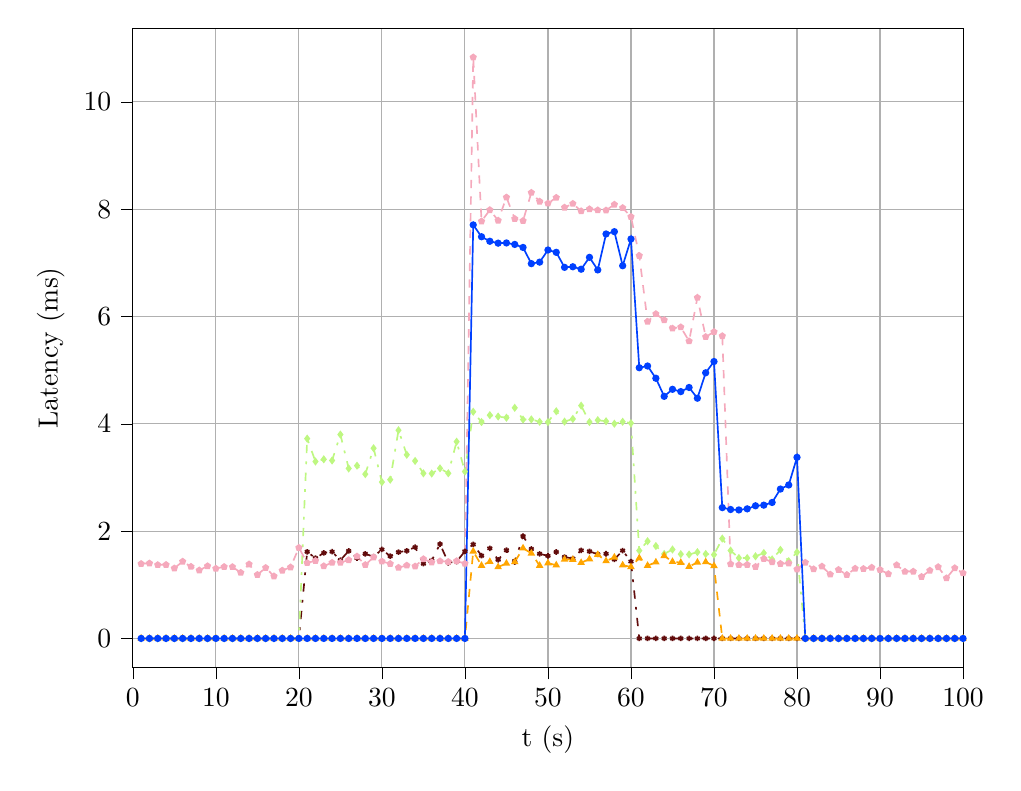
\begin{tikzpicture}

\definecolor{blue064255}{RGB}{0,64,255}
\definecolor{darkgrey176}{RGB}{176,176,176}
\definecolor{lightpink245169188}{RGB}{245,169,188}
\definecolor{maroon971111}{RGB}{97,11,11}
\definecolor{orange}{RGB}{255,165,0}
\definecolor{palegreen190247129}{RGB}{190,247,129}

\begin{axis}[
height=0.8\textwidth,
tick align=outside,
tick pos=left,
width=\textwidth,
x grid style={darkgrey176},
xlabel={t (s)},
xmajorgrids,
xmin=0, xmax=100,
xtick style={color=black},
y grid style={darkgrey176},
ylabel={Latency (ms)},
ymajorgrids,
ymin=-0.54155, ymax=11.37255,
ytick style={color=black}
]
\addplot [semithick, maroon971111, dash pattern=on 1pt off 3pt on 3pt off 3pt, mark=asterisk, mark size=1, mark options={solid}]
table {%
1 0
2 0
3 0
4 0
5 0
6 0
7 0
8 0
9 0
10 0
11 0
12 0
13 0
14 0
15 0
16 0
17 0
18 0
19 0
20 0
21 1.615
22 1.496
23 1.593
24 1.616
25 1.459
26 1.63
27 1.497
28 1.577
29 1.523
30 1.658
31 1.533
32 1.608
33 1.633
34 1.701
35 1.393
36 1.451
37 1.759
38 1.41
39 1.433
40 1.624
41 1.752
42 1.542
43 1.68
44 1.465
45 1.644
46 1.422
47 1.907
48 1.667
49 1.577
50 1.539
51 1.611
52 1.517
53 1.488
54 1.643
55 1.623
56 1.568
57 1.578
58 1.473
59 1.637
60 1.433
61 0
62 0
63 0
64 0
65 0
66 0
67 0
68 0
69 0
70 0
71 0
72 0
73 0
74 0
75 0
76 0
77 0
78 0
79 0
80 0
81 0
82 0
83 0
84 0
85 0
86 0
87 0
88 0
89 0
90 0
91 0
92 0
93 0
94 0
95 0
96 0
97 0
98 0
99 0
100 0
};
\addplot [semithick, palegreen190247129, dash pattern=on 1pt off 3pt on 3pt off 3pt, mark=diamond*, mark size=1, mark options={solid}]
table {%
1 0
2 0
3 0
4 0
5 0
6 0
7 0
8 0
9 0
10 0
11 0
12 0
13 0
14 0
15 0
16 0
17 0
18 0
19 0
20 0
21 3.724
22 3.297
23 3.338
24 3.316
25 3.8
26 3.168
27 3.22
28 3.062
29 3.545
30 2.914
31 2.959
32 3.88
33 3.423
34 3.308
35 3.077
36 3.073
37 3.17
38 3.078
39 3.667
40 3.11
41 4.225
42 4.032
43 4.161
44 4.136
45 4.114
46 4.298
47 4.079
48 4.082
49 4.038
50 4.032
51 4.234
52 4.041
53 4.091
54 4.339
55 4.033
56 4.068
57 4.047
58 4.002
59 4.038
60 4.012
61 1.637
62 1.812
63 1.722
64 1.575
65 1.657
66 1.571
67 1.565
68 1.608
69 1.574
70 1.561
71 1.861
72 1.638
73 1.499
74 1.498
75 1.531
76 1.592
77 1.474
78 1.651
79 1.44
80 1.607
81 0
82 0
83 0
84 0
85 0
86 0
87 0
88 0
89 0
90 0
91 0
92 0
93 0
94 0
95 0
96 0
97 0
98 0
99 0
100 0
};
\addplot [semithick, orange, dashed, mark=triangle*, mark size=1, mark options={solid}]
table {%
1 0
2 0
3 0
4 0
5 0
6 0
7 0
8 0
9 0
10 0
11 0
12 0
13 0
14 0
15 0
16 0
17 0
18 0
19 0
20 0
21 0
22 0
23 0
24 0
25 0
26 0
27 0
28 0
29 0
30 0
31 0
32 0
33 0
34 0
35 0
36 0
37 0
38 0
39 0
40 0
41 1.624
42 1.358
43 1.429
44 1.331
45 1.398
46 1.424
47 1.682
48 1.586
49 1.357
50 1.403
51 1.366
52 1.473
53 1.468
54 1.411
55 1.479
56 1.56
57 1.443
58 1.512
59 1.365
60 1.333
61 1.497
62 1.357
63 1.42
64 1.54
65 1.43
66 1.413
67 1.338
68 1.417
69 1.424
70 1.352
71 0
72 0
73 0
74 0
75 0
76 0
77 0
78 0
79 0
80 0
81 0
82 0
83 0
84 0
85 0
86 0
87 0
88 0
89 0
90 0
91 0
92 0
93 0
94 0
95 0
96 0
97 0
98 0
99 0
100 0
};
\addplot [semithick, lightpink245169188, dashed, mark=pentagon*, mark size=1, mark options={solid}]
table {%
1 1.391
2 1.4
3 1.37
4 1.373
5 1.308
6 1.434
7 1.338
8 1.27
9 1.349
10 1.303
11 1.335
12 1.333
13 1.226
14 1.383
15 1.187
16 1.317
17 1.16
18 1.267
19 1.327
20 1.691
21 1.408
22 1.448
23 1.349
24 1.413
25 1.412
26 1.462
27 1.53
28 1.371
29 1.513
30 1.436
31 1.392
32 1.32
33 1.361
34 1.344
35 1.48
36 1.42
37 1.44
38 1.429
39 1.443
40 1.395
41 10.831
42 7.775
43 7.986
44 7.79
45 8.221
46 7.821
47 7.784
48 8.308
49 8.144
50 8.108
51 8.215
52 8.032
53 8.103
54 7.964
55 8.002
56 7.982
57 7.979
58 8.087
59 8.025
60 7.859
61 7.133
62 5.905
63 6.048
64 5.934
65 5.778
66 5.802
67 5.54
68 6.352
69 5.621
70 5.714
71 5.637
72 1.386
73 1.371
74 1.374
75 1.336
76 1.484
77 1.425
78 1.393
79 1.399
80 1.289
81 1.415
82 1.292
83 1.343
84 1.193
85 1.281
86 1.186
87 1.303
88 1.298
89 1.322
90 1.28
91 1.202
92 1.368
93 1.245
94 1.248
95 1.15
96 1.267
97 1.332
98 1.124
99 1.312
100 1.217
};
\addplot [semithick, blue064255, mark=*, mark size=1, mark options={solid}]
table {%
1 0
2 0
3 0
4 0
5 0
6 0
7 0
8 0
9 0
10 0
11 0
12 0
13 0
14 0
15 0
16 0
17 0
18 0
19 0
20 0
21 0
22 0
23 0
24 0
25 0
26 0
27 0
28 0
29 0
30 0
31 0
32 0
33 0
34 0
35 0
36 0
37 0
38 0
39 0
40 0
41 7.707
42 7.486
43 7.402
44 7.367
45 7.371
46 7.343
47 7.287
48 6.985
49 7.013
50 7.239
51 7.196
52 6.916
53 6.927
54 6.881
55 7.102
56 6.868
57 7.538
58 7.581
59 6.946
60 7.444
61 5.045
62 5.077
63 4.849
64 4.512
65 4.643
66 4.6
67 4.677
68 4.477
69 4.951
70 5.161
71 2.438
72 2.403
73 2.395
74 2.415
75 2.472
76 2.484
77 2.534
78 2.784
79 2.86
80 3.375
81 0
82 0
83 0
84 0
85 0
86 0
87 0
88 0
89 0
90 0
91 0
92 0
93 0
94 0
95 0
96 0
97 0
98 0
99 0
100 0
};
\end{axis}

\end{tikzpicture}

        \hspace*{2.75em}
        \centering \small (f) \gls{hctns}: Latency Evolution.
    \end{minipage}
    \vspace*{0.25em}

    % SEGUNDA LEYENDA
    \vspace{0.5em} 
    \includegraphics[width=0.8\textwidth]{figures/results/ExperimentA/legend_tn.pdf}
    \vspace{0.3em}
    
    % TERCERA FILA
    \begin{minipage}[t]{0.3\textwidth}
        \centering
        % This file was created with tikzplotlib v0.10.1.
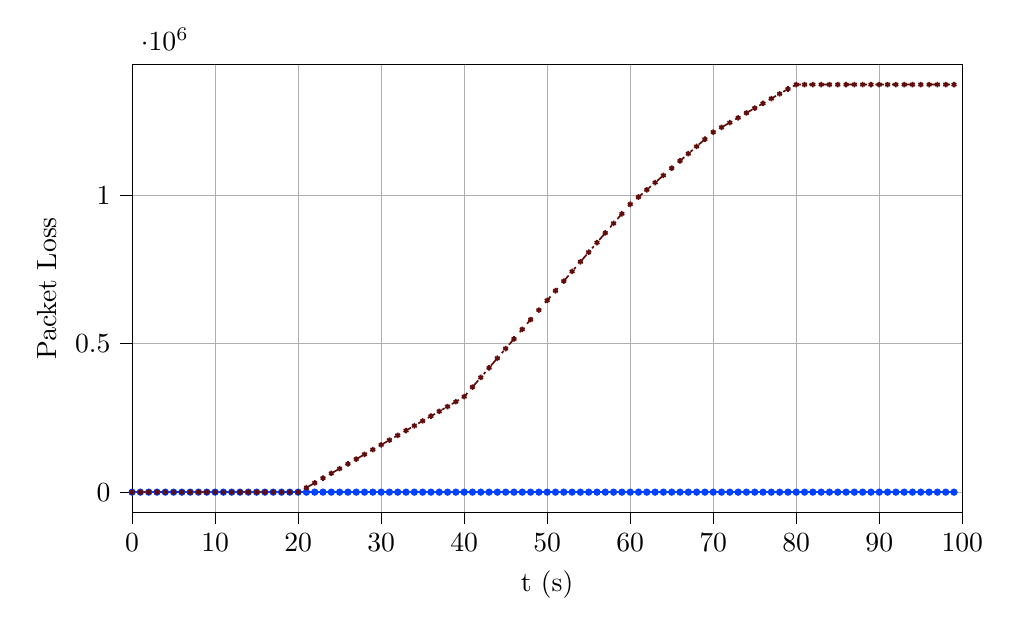
\begin{tikzpicture}

\definecolor{blue064255}{RGB}{0,64,255}
\definecolor{darkgrey176}{RGB}{176,176,176}
\definecolor{maroon971111}{RGB}{97,11,11}

\begin{axis}[
height=0.6\textwidth,
tick align=outside,
tick pos=left,
width=\textwidth,
x grid style={darkgrey176},
xlabel={t (s)},
xmajorgrids,
xmin=0, xmax=100,
xtick style={color=black},
y grid style={darkgrey176},
ylabel={Packet Loss},
ymajorgrids,
ymin=-68652.2, ymax=1441696.2,
ytick style={color=black}
]
\addplot [semithick, blue064255, mark=*, mark size=1, mark options={solid}]
table {%
0 0
1 0
2 0
3 0
4 0
5 0
6 0
7 0
8 0
9 0
10 0
11 0
12 0
13 0
14 0
15 0
16 0
17 0
18 0
19 0
20 0
21 0
22 0
23 0
24 0
25 0
26 0
27 0
28 0
29 0
30 0
31 0
32 0
33 0
34 0
35 0
36 0
37 0
38 0
39 0
40 0
41 0
42 0
43 0
44 0
45 0
46 0
47 0
48 0
49 0
50 0
51 0
52 0
53 0
54 0
55 0
56 0
57 0
58 0
59 0
60 0
61 0
62 0
63 0
64 0
65 0
66 0
67 0
68 0
69 0
70 0
71 0
72 0
73 0
74 0
75 0
76 0
77 0
78 0
79 0
80 0
81 0
82 0
83 0
84 0
85 0
86 0
87 0
88 0
89 0
90 0
91 0
92 0
93 0
94 0
95 0
96 0
97 0
98 0
99 0
};
\addplot [semithick, maroon971111, dash pattern=on 1pt off 3pt on 3pt off 3pt, mark=asterisk, mark size=1, mark options={solid}]
table {%
0 0
1 0
2 0
3 0
4 0
5 0
6 0
7 0
8 0
9 0
10 0
11 0
12 0
13 0
14 0
15 0
16 0
17 0
18 0
19 0
20 0
21 15137
22 31016
23 47111
24 63173
25 79182
26 95159
27 111177
28 127332
29 143342
30 159332
31 175350
32 191424
33 207498
34 223744
35 239981
36 256053
37 272294
38 288456
39 304614
40 321503
41 353955
42 386445
43 418780
44 451303
45 483731
46 516225
47 548690
48 581026
49 613490
50 645964
51 678445
52 710954
53 743437
54 775956
55 808313
56 840751
57 873269
58 905591
59 937842
60 969918
61 994275
62 1018586
63 1042858
64 1067219
65 1091574
66 1115942
67 1140269
68 1164638
69 1188976
70 1212696
71 1228881
72 1244913
73 1261144
74 1277373
75 1293595
76 1309729
77 1325940
78 1342022
79 1358107
80 1373044
81 1373044
82 1373044
83 1373044
84 1373044
85 1373044
86 1373044
87 1373044
88 1373044
89 1373044
90 1373044
91 1373044
92 1373044
93 1373044
94 1373044
95 1373044
96 1373044
97 1373044
98 1373044
99 1373044
};
\end{axis}

\end{tikzpicture}

        \hspace*{0.5em}   
        \centering \small (g) IETF: Packet Loss in output PE port.
    \end{minipage}
    \vspace*{0.25cm}
    \hfill
    \begin{minipage}[t]{0.3\textwidth}
        \centering
        % This file was created with tikzplotlib v0.10.1.
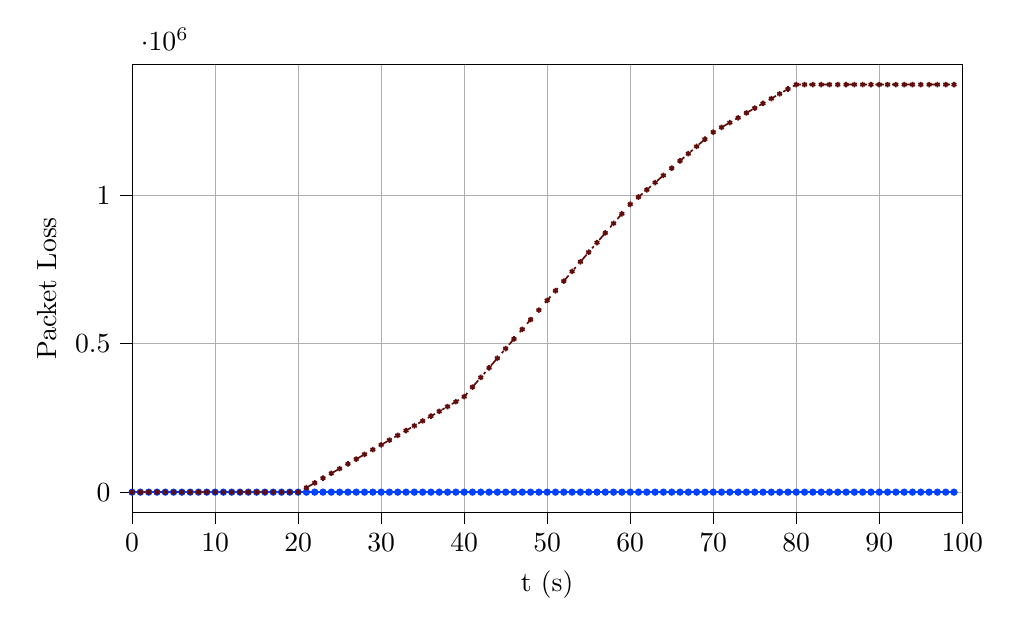
\begin{tikzpicture}

\definecolor{blue064255}{RGB}{0,64,255}
\definecolor{darkgrey176}{RGB}{176,176,176}
\definecolor{maroon971111}{RGB}{97,11,11}

\begin{axis}[
height=0.6\textwidth,
tick align=outside,
tick pos=left,
width=\textwidth,
x grid style={darkgrey176},
xlabel={t (s)},
xmajorgrids,
xmin=0, xmax=100,
xtick style={color=black},
y grid style={darkgrey176},
ylabel={Packet Loss},
ymajorgrids,
ymin=-68652.2, ymax=1441696.2,
ytick style={color=black}
]
\addplot [semithick, blue064255, mark=*, mark size=1, mark options={solid}]
table {%
0 0
1 0
2 0
3 0
4 0
5 0
6 0
7 0
8 0
9 0
10 0
11 0
12 0
13 0
14 0
15 0
16 0
17 0
18 0
19 0
20 0
21 0
22 0
23 0
24 0
25 0
26 0
27 0
28 0
29 0
30 0
31 0
32 0
33 0
34 0
35 0
36 0
37 0
38 0
39 0
40 0
41 0
42 0
43 0
44 0
45 0
46 0
47 0
48 0
49 0
50 0
51 0
52 0
53 0
54 0
55 0
56 0
57 0
58 0
59 0
60 0
61 0
62 0
63 0
64 0
65 0
66 0
67 0
68 0
69 0
70 0
71 0
72 0
73 0
74 0
75 0
76 0
77 0
78 0
79 0
80 0
81 0
82 0
83 0
84 0
85 0
86 0
87 0
88 0
89 0
90 0
91 0
92 0
93 0
94 0
95 0
96 0
97 0
98 0
99 0
};
\addplot [semithick, maroon971111, dash pattern=on 1pt off 3pt on 3pt off 3pt, mark=asterisk, mark size=1, mark options={solid}]
table {%
0 0
1 0
2 0
3 0
4 0
5 0
6 0
7 0
8 0
9 0
10 0
11 0
12 0
13 0
14 0
15 0
16 0
17 0
18 0
19 0
20 0
21 15137
22 31016
23 47111
24 63173
25 79182
26 95159
27 111177
28 127332
29 143342
30 159332
31 175350
32 191424
33 207498
34 223744
35 239981
36 256053
37 272294
38 288456
39 304614
40 321503
41 353955
42 386445
43 418780
44 451303
45 483731
46 516225
47 548690
48 581026
49 613490
50 645964
51 678445
52 710954
53 743437
54 775956
55 808313
56 840751
57 873269
58 905591
59 937842
60 969918
61 994275
62 1018586
63 1042858
64 1067219
65 1091574
66 1115942
67 1140269
68 1164638
69 1188976
70 1212696
71 1228881
72 1244913
73 1261144
74 1277373
75 1293595
76 1309729
77 1325940
78 1342022
79 1358107
80 1373044
81 1373044
82 1373044
83 1373044
84 1373044
85 1373044
86 1373044
87 1373044
88 1373044
89 1373044
90 1373044
91 1373044
92 1373044
93 1373044
94 1373044
95 1373044
96 1373044
97 1373044
98 1373044
99 1373044
};
\end{axis}

\end{tikzpicture}

        \hspace*{1.75em}
        \centering \small (h) \cite{Lin2021}: Packet Loss in output PE port.
    \end{minipage}
    \vspace*{0.25cm}
    \hfill
    \begin{minipage}[t]{0.3\textwidth} % Cuarta subfigura
        \centering
        % This file was created with tikzplotlib v0.10.1.
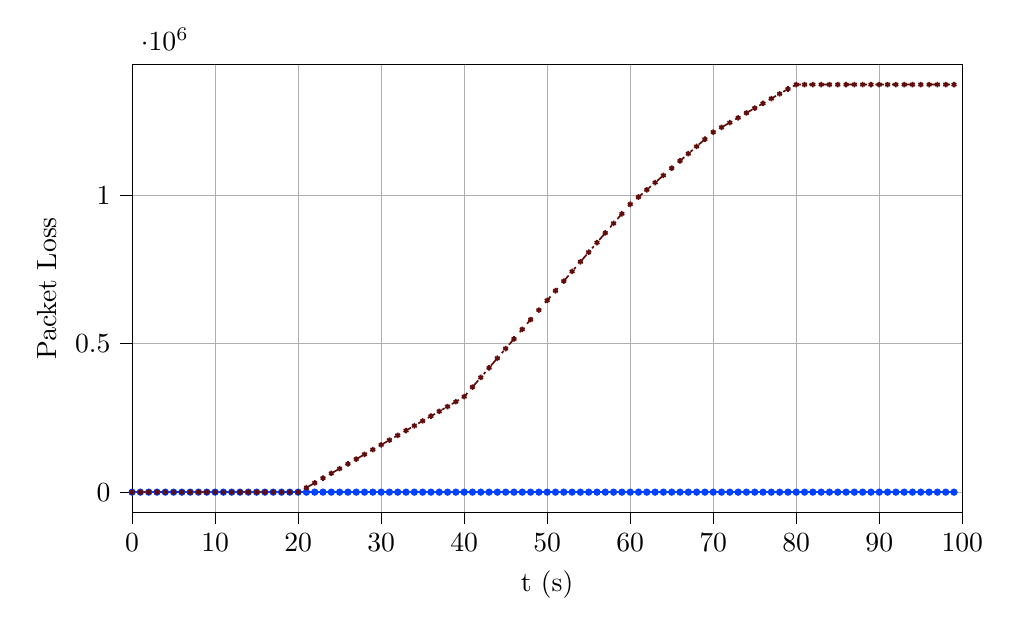
\begin{tikzpicture}

\definecolor{blue064255}{RGB}{0,64,255}
\definecolor{darkgrey176}{RGB}{176,176,176}
\definecolor{maroon971111}{RGB}{97,11,11}

\begin{axis}[
height=0.6\textwidth,
tick align=outside,
tick pos=left,
width=\textwidth,
x grid style={darkgrey176},
xlabel={t (s)},
xmajorgrids,
xmin=0, xmax=100,
xtick style={color=black},
y grid style={darkgrey176},
ylabel={Packet Loss},
ymajorgrids,
ymin=-68652.2, ymax=1441696.2,
ytick style={color=black}
]
\addplot [semithick, blue064255, mark=*, mark size=1, mark options={solid}]
table {%
0 0
1 0
2 0
3 0
4 0
5 0
6 0
7 0
8 0
9 0
10 0
11 0
12 0
13 0
14 0
15 0
16 0
17 0
18 0
19 0
20 0
21 0
22 0
23 0
24 0
25 0
26 0
27 0
28 0
29 0
30 0
31 0
32 0
33 0
34 0
35 0
36 0
37 0
38 0
39 0
40 0
41 0
42 0
43 0
44 0
45 0
46 0
47 0
48 0
49 0
50 0
51 0
52 0
53 0
54 0
55 0
56 0
57 0
58 0
59 0
60 0
61 0
62 0
63 0
64 0
65 0
66 0
67 0
68 0
69 0
70 0
71 0
72 0
73 0
74 0
75 0
76 0
77 0
78 0
79 0
80 0
81 0
82 0
83 0
84 0
85 0
86 0
87 0
88 0
89 0
90 0
91 0
92 0
93 0
94 0
95 0
96 0
97 0
98 0
99 0
};
\addplot [semithick, maroon971111, dash pattern=on 1pt off 3pt on 3pt off 3pt, mark=asterisk, mark size=1, mark options={solid}]
table {%
0 0
1 0
2 0
3 0
4 0
5 0
6 0
7 0
8 0
9 0
10 0
11 0
12 0
13 0
14 0
15 0
16 0
17 0
18 0
19 0
20 0
21 15137
22 31016
23 47111
24 63173
25 79182
26 95159
27 111177
28 127332
29 143342
30 159332
31 175350
32 191424
33 207498
34 223744
35 239981
36 256053
37 272294
38 288456
39 304614
40 321503
41 353955
42 386445
43 418780
44 451303
45 483731
46 516225
47 548690
48 581026
49 613490
50 645964
51 678445
52 710954
53 743437
54 775956
55 808313
56 840751
57 873269
58 905591
59 937842
60 969918
61 994275
62 1018586
63 1042858
64 1067219
65 1091574
66 1115942
67 1140269
68 1164638
69 1188976
70 1212696
71 1228881
72 1244913
73 1261144
74 1277373
75 1293595
76 1309729
77 1325940
78 1342022
79 1358107
80 1373044
81 1373044
82 1373044
83 1373044
84 1373044
85 1373044
86 1373044
87 1373044
88 1373044
89 1373044
90 1373044
91 1373044
92 1373044
93 1373044
94 1373044
95 1373044
96 1373044
97 1373044
98 1373044
99 1373044
};
\end{axis}

\end{tikzpicture}

        \hspace*{0.75em}
        \centering \small (i) \gls{hctns}: Packet Loss in output PE port.
    \end{minipage}
    \vspace*{0.25cm}
    % CUARTA FILA
    \begin{minipage}[t]{0.3\textwidth}
        \centering
        % This file was created with tikzplotlib v0.10.1.
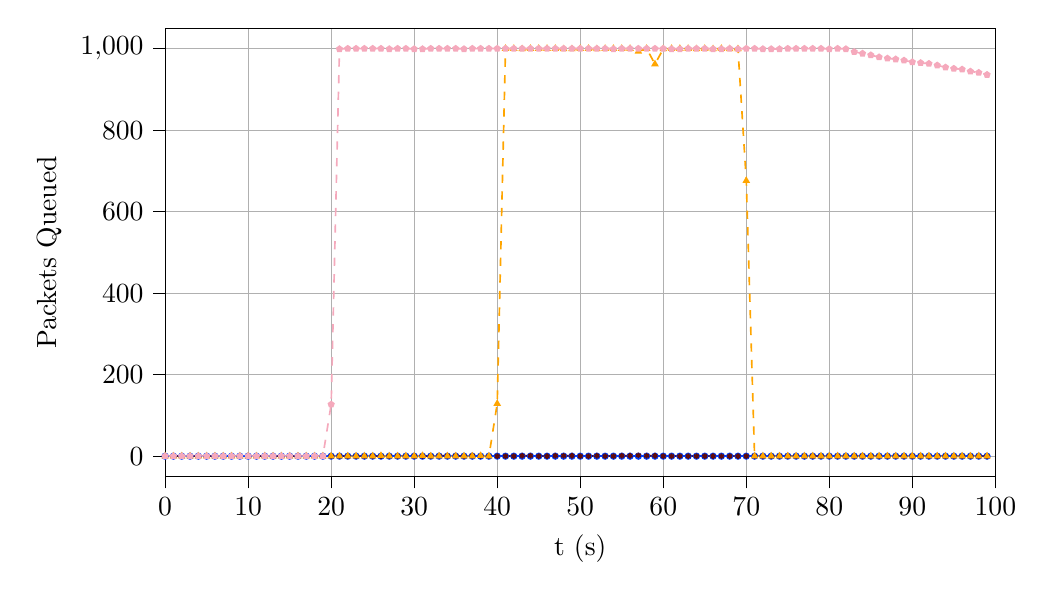
\begin{tikzpicture}

\definecolor{blue064255}{RGB}{0,64,255}
\definecolor{darkgrey176}{RGB}{176,176,176}
\definecolor{lightpink245169188}{RGB}{245,169,188}
\definecolor{maroon971111}{RGB}{97,11,11}
\definecolor{orange}{RGB}{255,165,0}

\begin{axis}[
height=0.6\textwidth,
tick align=outside,
tick pos=left,
width=\textwidth,
x grid style={darkgrey176},
xlabel={t (s)},
xmajorgrids,
xmin=0, xmax=100,
xtick style={color=black},
y grid style={darkgrey176},
ylabel={Packets Queued},
ymajorgrids,
ymin=-50, ymax=1050,
ytick style={color=black}
]
\addplot [semithick, blue064255, mark=*, mark size=1, mark options={solid}]
table {%
0 0
1 0
2 0
3 0
4 0
5 0
6 0
7 0
8 0
9 0
10 0
11 0
12 0
13 0
14 0
15 0
16 0
17 0
18 0
19 0
20 0
21 0
22 0
23 0
24 0
25 0
26 0
27 0
28 0
29 0
30 0
31 0
32 0
33 0
34 0
35 0
36 0
37 0
38 0
39 0
40 0
41 0
42 0
43 0
44 0
45 0
46 0
47 0
48 0
49 0
50 0
51 0
52 0
53 0
54 0
55 0
56 0
57 0
58 0
59 0
60 0
61 0
62 0
63 0
64 0
65 0
66 0
67 0
68 0
69 0
70 0
71 0
72 0
73 0
74 0
75 0
76 0
77 0
78 0
79 0
80 0
81 0
82 0
83 0
84 0
85 0
86 0
87 0
88 0
89 0
90 0
91 0
92 0
93 0
94 0
95 0
96 0
97 0
98 0
99 0
};
\addplot [semithick, maroon971111, dash pattern=on 1pt off 3pt on 3pt off 3pt, mark=asterisk, mark size=1, mark options={solid}]
table {%
0 0
1 0
2 0
3 0
4 0
5 0
6 0
7 0
8 0
9 0
10 0
11 0
12 0
13 0
14 0
15 0
16 0
17 0
18 0
19 0
20 0
21 0
22 0
23 0
24 0
25 0
26 0
27 0
28 0
29 0
30 0
31 0
32 0
33 1
34 1
35 1
36 0
37 1
38 0
39 0
40 0
41 0
42 0
43 1
44 1
45 0
46 0
47 1
48 1
49 1
50 0
51 0
52 1
53 0
54 0
55 1
56 1
57 2
58 1
59 1
60 0
61 0
62 0
63 0
64 0
65 0
66 0
67 0
68 0
69 0
70 0
71 0
72 0
73 0
74 0
75 0
76 0
77 0
78 0
79 0
80 0
81 0
82 0
83 0
84 0
85 0
86 0
87 0
88 0
89 0
90 0
91 0
92 0
93 0
94 0
95 0
96 0
97 0
98 0
99 0
};
\addplot [semithick, orange, dashed, mark=triangle*, mark size=1, mark options={solid}]
table {%
0 0
1 0
2 0
3 0
4 0
5 0
6 0
7 0
8 0
9 0
10 0
11 0
12 0
13 0
14 0
15 0
16 0
17 0
18 0
19 0
20 0
21 0
22 0
23 0
24 0
25 0
26 1
27 0
28 0
29 0
30 0
31 1
32 0
33 0
34 0
35 0
36 0
37 0
38 1
39 0
40 129
41 1000
42 1000
43 999
44 1000
45 1000
46 1000
47 1000
48 999
49 999
50 1000
51 1000
52 999
53 1000
54 1000
55 1000
56 1000
57 993
58 1000
59 962
60 999
61 1000
62 1000
63 1000
64 999
65 1000
66 999
67 1000
68 999
69 999
70 676
71 0
72 0
73 0
74 0
75 0
76 0
77 0
78 0
79 0
80 0
81 0
82 0
83 0
84 0
85 0
86 0
87 0
88 0
89 0
90 0
91 0
92 0
93 0
94 0
95 0
96 0
97 0
98 0
99 0
};
\addplot [semithick, lightpink245169188, dashed, mark=pentagon*, mark size=1, mark options={solid}]
table {%
0 0
1 0
2 0
3 0
4 0
5 0
6 0
7 0
8 0
9 0
10 0
11 0
12 0
13 0
14 0
15 0
16 0
17 0
18 0
19 0
20 127
21 999
22 1000
23 1000
24 1000
25 1000
26 1000
27 999
28 1000
29 1000
30 999
31 999
32 1000
33 1000
34 1000
35 1000
36 999
37 1000
38 1000
39 1000
40 1000
41 1000
42 1000
43 1000
44 1000
45 1000
46 1000
47 1000
48 1000
49 1000
50 1000
51 1000
52 1000
53 1000
54 999
55 1000
56 1000
57 1000
58 1000
59 1000
60 1000
61 999
62 999
63 1000
64 1000
65 1000
66 999
67 999
68 1000
69 999
70 1000
71 1000
72 999
73 999
74 999
75 1000
76 1000
77 1000
78 1000
79 1000
80 999
81 1000
82 999
83 992
84 988
85 984
86 979
87 976
88 974
89 971
90 967
91 965
92 963
93 959
94 954
95 951
96 949
97 944
98 941
99 936
};
\end{axis}

\end{tikzpicture}

        \hspace*{0.4em}   
        \centering \small (j) IETF: Packets Queued in output PE port.
    \end{minipage}
    \hfill
    \begin{minipage}[t]{0.3\textwidth}
        \centering
        % This file was created with tikzplotlib v0.10.1.
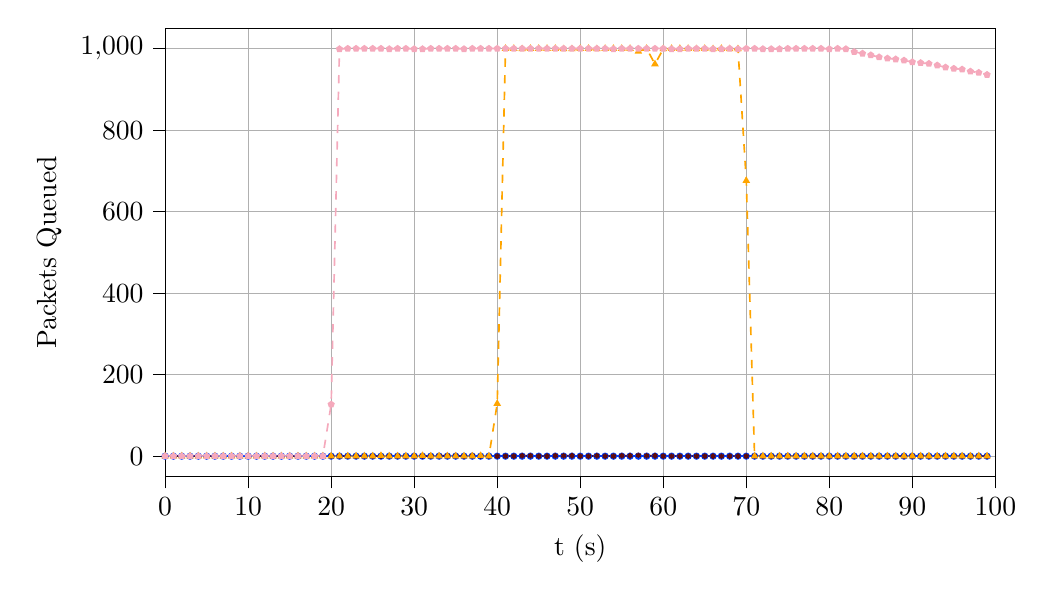
\begin{tikzpicture}

\definecolor{blue064255}{RGB}{0,64,255}
\definecolor{darkgrey176}{RGB}{176,176,176}
\definecolor{lightpink245169188}{RGB}{245,169,188}
\definecolor{maroon971111}{RGB}{97,11,11}
\definecolor{orange}{RGB}{255,165,0}

\begin{axis}[
height=0.6\textwidth,
tick align=outside,
tick pos=left,
width=\textwidth,
x grid style={darkgrey176},
xlabel={t (s)},
xmajorgrids,
xmin=0, xmax=100,
xtick style={color=black},
y grid style={darkgrey176},
ylabel={Packets Queued},
ymajorgrids,
ymin=-50, ymax=1050,
ytick style={color=black}
]
\addplot [semithick, blue064255, mark=*, mark size=1, mark options={solid}]
table {%
0 0
1 0
2 0
3 0
4 0
5 0
6 0
7 0
8 0
9 0
10 0
11 0
12 0
13 0
14 0
15 0
16 0
17 0
18 0
19 0
20 0
21 0
22 0
23 0
24 0
25 0
26 0
27 0
28 0
29 0
30 0
31 0
32 0
33 0
34 0
35 0
36 0
37 0
38 0
39 0
40 0
41 0
42 0
43 0
44 0
45 0
46 0
47 0
48 0
49 0
50 0
51 0
52 0
53 0
54 0
55 0
56 0
57 0
58 0
59 0
60 0
61 0
62 0
63 0
64 0
65 0
66 0
67 0
68 0
69 0
70 0
71 0
72 0
73 0
74 0
75 0
76 0
77 0
78 0
79 0
80 0
81 0
82 0
83 0
84 0
85 0
86 0
87 0
88 0
89 0
90 0
91 0
92 0
93 0
94 0
95 0
96 0
97 0
98 0
99 0
};
\addplot [semithick, maroon971111, dash pattern=on 1pt off 3pt on 3pt off 3pt, mark=asterisk, mark size=1, mark options={solid}]
table {%
0 0
1 0
2 0
3 0
4 0
5 0
6 0
7 0
8 0
9 0
10 0
11 0
12 0
13 0
14 0
15 0
16 0
17 0
18 0
19 0
20 0
21 0
22 0
23 0
24 0
25 0
26 0
27 0
28 0
29 0
30 0
31 0
32 0
33 1
34 1
35 1
36 0
37 1
38 0
39 0
40 0
41 0
42 0
43 1
44 1
45 0
46 0
47 1
48 1
49 1
50 0
51 0
52 1
53 0
54 0
55 1
56 1
57 2
58 1
59 1
60 0
61 0
62 0
63 0
64 0
65 0
66 0
67 0
68 0
69 0
70 0
71 0
72 0
73 0
74 0
75 0
76 0
77 0
78 0
79 0
80 0
81 0
82 0
83 0
84 0
85 0
86 0
87 0
88 0
89 0
90 0
91 0
92 0
93 0
94 0
95 0
96 0
97 0
98 0
99 0
};
\addplot [semithick, orange, dashed, mark=triangle*, mark size=1, mark options={solid}]
table {%
0 0
1 0
2 0
3 0
4 0
5 0
6 0
7 0
8 0
9 0
10 0
11 0
12 0
13 0
14 0
15 0
16 0
17 0
18 0
19 0
20 0
21 0
22 0
23 0
24 0
25 0
26 1
27 0
28 0
29 0
30 0
31 1
32 0
33 0
34 0
35 0
36 0
37 0
38 1
39 0
40 129
41 1000
42 1000
43 999
44 1000
45 1000
46 1000
47 1000
48 999
49 999
50 1000
51 1000
52 999
53 1000
54 1000
55 1000
56 1000
57 993
58 1000
59 962
60 999
61 1000
62 1000
63 1000
64 999
65 1000
66 999
67 1000
68 999
69 999
70 676
71 0
72 0
73 0
74 0
75 0
76 0
77 0
78 0
79 0
80 0
81 0
82 0
83 0
84 0
85 0
86 0
87 0
88 0
89 0
90 0
91 0
92 0
93 0
94 0
95 0
96 0
97 0
98 0
99 0
};
\addplot [semithick, lightpink245169188, dashed, mark=pentagon*, mark size=1, mark options={solid}]
table {%
0 0
1 0
2 0
3 0
4 0
5 0
6 0
7 0
8 0
9 0
10 0
11 0
12 0
13 0
14 0
15 0
16 0
17 0
18 0
19 0
20 127
21 999
22 1000
23 1000
24 1000
25 1000
26 1000
27 999
28 1000
29 1000
30 999
31 999
32 1000
33 1000
34 1000
35 1000
36 999
37 1000
38 1000
39 1000
40 1000
41 1000
42 1000
43 1000
44 1000
45 1000
46 1000
47 1000
48 1000
49 1000
50 1000
51 1000
52 1000
53 1000
54 999
55 1000
56 1000
57 1000
58 1000
59 1000
60 1000
61 999
62 999
63 1000
64 1000
65 1000
66 999
67 999
68 1000
69 999
70 1000
71 1000
72 999
73 999
74 999
75 1000
76 1000
77 1000
78 1000
79 1000
80 999
81 1000
82 999
83 992
84 988
85 984
86 979
87 976
88 974
89 971
90 967
91 965
92 963
93 959
94 954
95 951
96 949
97 944
98 941
99 936
};
\end{axis}

\end{tikzpicture}

        \hspace*{0.5em}
        \centering \small (k) \cite{Lin2021}: Packets Queued in output PE port.
    \end{minipage}
    \hfill
    \begin{minipage}[t]{0.3\textwidth} % Cuarta subfigura
        \centering
        % This file was created with tikzplotlib v0.10.1.
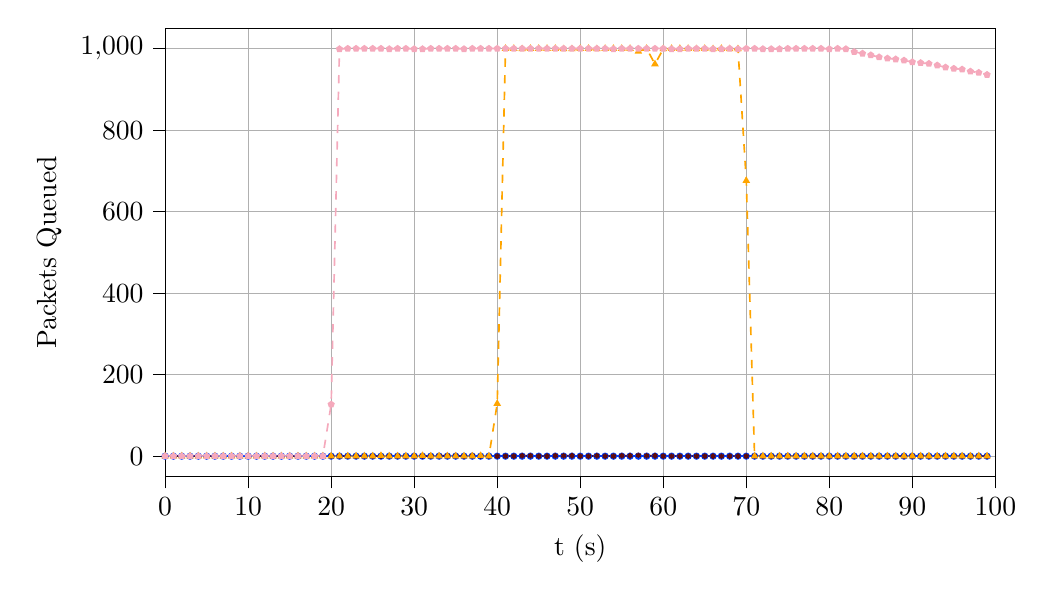
\begin{tikzpicture}

\definecolor{blue064255}{RGB}{0,64,255}
\definecolor{darkgrey176}{RGB}{176,176,176}
\definecolor{lightpink245169188}{RGB}{245,169,188}
\definecolor{maroon971111}{RGB}{97,11,11}
\definecolor{orange}{RGB}{255,165,0}

\begin{axis}[
height=0.6\textwidth,
tick align=outside,
tick pos=left,
width=\textwidth,
x grid style={darkgrey176},
xlabel={t (s)},
xmajorgrids,
xmin=0, xmax=100,
xtick style={color=black},
y grid style={darkgrey176},
ylabel={Packets Queued},
ymajorgrids,
ymin=-50, ymax=1050,
ytick style={color=black}
]
\addplot [semithick, blue064255, mark=*, mark size=1, mark options={solid}]
table {%
0 0
1 0
2 0
3 0
4 0
5 0
6 0
7 0
8 0
9 0
10 0
11 0
12 0
13 0
14 0
15 0
16 0
17 0
18 0
19 0
20 0
21 0
22 0
23 0
24 0
25 0
26 0
27 0
28 0
29 0
30 0
31 0
32 0
33 0
34 0
35 0
36 0
37 0
38 0
39 0
40 0
41 0
42 0
43 0
44 0
45 0
46 0
47 0
48 0
49 0
50 0
51 0
52 0
53 0
54 0
55 0
56 0
57 0
58 0
59 0
60 0
61 0
62 0
63 0
64 0
65 0
66 0
67 0
68 0
69 0
70 0
71 0
72 0
73 0
74 0
75 0
76 0
77 0
78 0
79 0
80 0
81 0
82 0
83 0
84 0
85 0
86 0
87 0
88 0
89 0
90 0
91 0
92 0
93 0
94 0
95 0
96 0
97 0
98 0
99 0
};
\addplot [semithick, maroon971111, dash pattern=on 1pt off 3pt on 3pt off 3pt, mark=asterisk, mark size=1, mark options={solid}]
table {%
0 0
1 0
2 0
3 0
4 0
5 0
6 0
7 0
8 0
9 0
10 0
11 0
12 0
13 0
14 0
15 0
16 0
17 0
18 0
19 0
20 0
21 0
22 0
23 0
24 0
25 0
26 0
27 0
28 0
29 0
30 0
31 0
32 0
33 1
34 1
35 1
36 0
37 1
38 0
39 0
40 0
41 0
42 0
43 1
44 1
45 0
46 0
47 1
48 1
49 1
50 0
51 0
52 1
53 0
54 0
55 1
56 1
57 2
58 1
59 1
60 0
61 0
62 0
63 0
64 0
65 0
66 0
67 0
68 0
69 0
70 0
71 0
72 0
73 0
74 0
75 0
76 0
77 0
78 0
79 0
80 0
81 0
82 0
83 0
84 0
85 0
86 0
87 0
88 0
89 0
90 0
91 0
92 0
93 0
94 0
95 0
96 0
97 0
98 0
99 0
};
\addplot [semithick, orange, dashed, mark=triangle*, mark size=1, mark options={solid}]
table {%
0 0
1 0
2 0
3 0
4 0
5 0
6 0
7 0
8 0
9 0
10 0
11 0
12 0
13 0
14 0
15 0
16 0
17 0
18 0
19 0
20 0
21 0
22 0
23 0
24 0
25 0
26 1
27 0
28 0
29 0
30 0
31 1
32 0
33 0
34 0
35 0
36 0
37 0
38 1
39 0
40 129
41 1000
42 1000
43 999
44 1000
45 1000
46 1000
47 1000
48 999
49 999
50 1000
51 1000
52 999
53 1000
54 1000
55 1000
56 1000
57 993
58 1000
59 962
60 999
61 1000
62 1000
63 1000
64 999
65 1000
66 999
67 1000
68 999
69 999
70 676
71 0
72 0
73 0
74 0
75 0
76 0
77 0
78 0
79 0
80 0
81 0
82 0
83 0
84 0
85 0
86 0
87 0
88 0
89 0
90 0
91 0
92 0
93 0
94 0
95 0
96 0
97 0
98 0
99 0
};
\addplot [semithick, lightpink245169188, dashed, mark=pentagon*, mark size=1, mark options={solid}]
table {%
0 0
1 0
2 0
3 0
4 0
5 0
6 0
7 0
8 0
9 0
10 0
11 0
12 0
13 0
14 0
15 0
16 0
17 0
18 0
19 0
20 127
21 999
22 1000
23 1000
24 1000
25 1000
26 1000
27 999
28 1000
29 1000
30 999
31 999
32 1000
33 1000
34 1000
35 1000
36 999
37 1000
38 1000
39 1000
40 1000
41 1000
42 1000
43 1000
44 1000
45 1000
46 1000
47 1000
48 1000
49 1000
50 1000
51 1000
52 1000
53 1000
54 999
55 1000
56 1000
57 1000
58 1000
59 1000
60 1000
61 999
62 999
63 1000
64 1000
65 1000
66 999
67 999
68 1000
69 999
70 1000
71 1000
72 999
73 999
74 999
75 1000
76 1000
77 1000
78 1000
79 1000
80 999
81 1000
82 999
83 992
84 988
85 984
86 979
87 976
88 974
89 971
90 967
91 965
92 963
93 959
94 954
95 951
96 949
97 944
98 941
99 936
};
\end{axis}

\end{tikzpicture}

        \hspace*{-0.2cm}
        \centering \small (l) \gls{hctns}: Packets Queued in output PE port.
    \end{minipage}
    \caption{Experiment A: \gls{ietf} and \cite{Lin2021} network slicing models versus \gls{hctns}.}
    \label{fig:expa-ietf-proposal}
\end{figure*}
}

Fig.~\ref{fig:expa-ietf-proposal} presents the results obtained with the \gls{ietf} network slicing model alongside the results achieved with~\rev{the \cite{Lin2021} model and} \gls{hctns}. As discussed below, significant differences in the \gls{qos} provided to the traffic flows are observed between the three approaches.  

In \textit{Interval 1}, only BE traffic is active, fully utilizing the available bandwidth (100\,Mbps of the link between the PE1 and the P routers). All traffic is admitted by the ingress policers in all the models (Figures~\ref{fig:expa-ietf-proposal}a, \ref{fig:expa-ietf-proposal}b and \ref{fig:expa-ietf-proposal}c). Since the accepted BE traffic does not exceed the link capacity, packet delay remains low (Figures~\ref{fig:expa-ietf-proposal}d, \ref{fig:expa-ietf-proposal}e and \ref{fig:expa-ietf-proposal}f), and no packets are lost (Figures~\ref{fig:expa-ietf-proposal}g, \ref{fig:expa-ietf-proposal}h  and \ref{fig:expa-ietf-proposal}i) or enqueued (Figures~\ref{fig:expa-ietf-proposal}j, \ref{fig:expa-ietf-proposal}k and \ref{fig:expa-ietf-proposal}l) in the output port of \gls{pe}1. For this interval, all models show the same behavior.

In \textit{Interval 2}, BE traffic from the \gls{embb} slice, along with video and telemetry traffic from the \gls{tod} slice simultaneously enter the transport network.
\rev{The \gls{ietf} and \gls{hctns} models, by utilizing hierarchical policers, not only ensure the configured \gls{cir} for each traffic flow but also guarantee it at the slice level. Consequently, even though BE traffic does not have explicit bandwidth guarantees, it belongs to the \gls{embb} slice, which has a \gls{cir} of 52.8\,Mbps. If no other traffic in the slice is using that bandwidth, BE traffic can take advantage of the slice's guaranteed bandwidth.
In the \gls{ietf} model, traffic classes with bandwidth guarantees cannot exceed their assigned \gls{cir}. As a result, video traffic is limited to 32\,Mbps, aligning with the \gls{cir} values defined in Table~\ref{tab:expa-params}. Similarly, telemetry traffic is restricted to 4 Mbps. However, the 100\,Mbps of BE traffic are accepted by the policer, therefore, the remaining bandwidth is fully utilized by BE traffic (achieving 64 Mbps of the bandwidth in the link between the PE1 and the P routers). However, in the \gls{hctns} model, all the active flows can consume part of the excess bandwidth exceeding their respective \glspl{cir}. \rev{The \gls{htb} Linux tool implementation, based on a \gls{drr} scheduler that we configured with equal quantum values for all leaf nodes, assigns the excess bandwidth, in this case, as follows: the telemetry and video classes receive an additional 5.6 Mbps, while the BE traffic, which is set without a \gls{cir}, consume the 52.8 Mbps allocated to the \gls{embb} slice.} On the other hand, in the~\cite{Lin2021} model, BE traffic is treated as an independent slice without any bandwidth guarantees. Consequently, in the \cite{Lin2021} model, traffic flows can secure their \gls{cir} bandwidth (the policer marks this traffic as ``green") and other traffic (BE and ``yellow" traffic, i.e., the traffic above the \gls{cir} and under the \gls{pir} of other flows) compete for the remaining available bandwidth, achieving a total of 54\,Mbps for video, 26\,Mbps for telemetry, and 20\,Mbps for BE traffic.}

The coarse-grained resource control plays a crucial role in achieving these results. Packet loss in the \gls{ietf} model occurs when traffic admitted by the ingress policer attempts to access a \gls{drr} queue that is already full, as shown in Fig.~\ref{fig:expa-ietf-proposal}j, in the egress port of \gls{pe}1. \rev{The same occurs with the \cite{Lin2021} model, where BE and ``yellow" packets wait in the lower priority queue, as shown in Fig.~\ref{fig:expa-ietf-proposal}k}. In contrast, the operation of the global policer in \gls{hctns} prevents packets from waiting in the output port queues of the \gls{pe}1 (Fig.~\ref{fig:expa-ietf-proposal}l). This is achieved because our fine-grained resource control mechanism only accepts traffic that can be processed within the transport network with \gls{qos} guarantees.

 As shown in Table~\ref{tab:expa-params}, the same quantums values were configured for the \gls{drr} queues of the \gls{ietf} and \gls{hctns} models, corresponding to \gls{tn} classes B, C, and D. This configuration does not apply to \gls{tn} class A, as this traffic class utilizes the priority queue within the coarse-grained resource control queuing system, \rev{neither to the queues implemented in the~\cite{Lin2021} model, since~\cite{Lin2021} uses two priority queues.} For the quantum values used in this experiment, and without traffic of \gls{tn} \gls{qos} class A, the packet scheduler can serve packets from the \gls{drr} queues at an average transmission rate of 33.3\,Mbps for each of the \gls{tn} \gls{qos} classes B, C and D, when there are packets of all these \gls{tn} classes waiting in the queues to be transmitted.  

During \textit{Interval 2} of the Experiment A, the \gls{ietf} \gls{drr} queue corresponding to the \gls{tn} \gls{qos} class B exclusively receives video traffic from the \gls{tod} slice at a rate of 32\,Mbps, which explains why packets from this flow are neither dropped nor enqueued (Figs.~\ref{fig:expa-ietf-proposal}g and~\ref{fig:expa-ietf-proposal}j). Similarly, the \gls{drr} queue assigned to \gls{tn} \gls{qos} class C receives telemetry traffic at a rate of 4\,Mbps, a rate that is also below the threshold of 33.3\,Mbps. The problem arises with BE traffic, which is enqueued in the \gls{drr} for the \gls{tn} class D. In this case, BE traffic is received at a rate of 100\,Mbps. As previously mentioned, when all \gls{drr} queues contain packets waiting for transmission, the packet scheduler can only serve packets at an average rate of 33.3\,Mbps per queue. However, since the video and telemetry rates remain below their thresholds, the BE traffic can utilize the remaining available bandwidth, achieving a transmission rate of 64\,Mbps. As BE traffic is admitted by the \gls{ietf} ingress policer at a rate of 100\,Mbps, which exceeds the available 64\,Mbps, packet losses occur, and some packets experience queuing delays. \rev{On the other hand, the \cite{Lin2021} model forwards all the ``green" traffic (i.e., traffic under \gls{cir}) to the highest priority queue. Since the sum of the \gls{cir} values of the current traffic, 34\,Mbps in this interval, is lower than the link capacity, packets are not enqueued nor dropped. However, this model forwards all ``yellow'' traffic (i.e., between \gls{cir} and \gls{pir} rate) and the BE traffic to the lowest priority queue. As a consequence, more traffic arrives at the lowest priority queue than it can handle, leading to queue filling and packet losses, as shown in Figs.~\ref{fig:expa-ietf-proposal}k and ~\ref{fig:expa-ietf-proposal}h}. In contrast to both the IETF and the~\cite{Lin2021} models, \gls{hctns} includes a global policer that limits the total traffic entering the \gls{tn}. This mechanism ensures that traffic does not exceed the global available bandwidth at the output of the \gls{pe}1 router. As a result, packets are not enqueued nor dropped, as illustrated in Figs.~\ref{fig:expa-ietf-proposal}l and ~\ref{fig:expa-ietf-proposal}i.

Queuing delays determine the packet delay measurements shown in Figs.~\ref{fig:expa-ietf-proposal}d, \ref{fig:expa-ietf-proposal}e and \ref{fig:expa-ietf-proposal}f. During \textit{Interval 2}, in the \gls{ietf} model, packets from the \gls{tod} slice are not significantly affected by queuing delays, because traffic is generated at rates below the threshold of 33.3\,Mbps \rev{and there is not other traffic in their associated \gls{tn} \gls{qos} classes}. However, BE traffic is accumulated (also discarded) in the \gls{drr} queue of the \gls{tn} class D. \rev{In the \cite{Lin2021} model, since all flows have packets marked as ``yellow'' by the ingress policer, the maximum latency experienced by a flow is determined by the waiting time of the lowest priority queue, leading to similar latencies for all flows as BE traffic, around 195\,ms.} In contrast, in our proposed model, packet delay is influenced by the waiting time in the queue associated with the input port. This waiting time depends on the token arrival rate defined for each traffic class, i.e., the speed at which tokens are received in the \textit{\gls{cir}} and \textit{\gls{pir}} buckets defined in Section~\ref{sec:proposal}.\ref{subsec:proposal-finegraine}. As soon as there are tokens available in these buckets, the packet waiting in the queue of the \gls{htb} can be transmitted to the switching fabric of the \gls{pe} router. 

\textit{Interval 3} is particularly insightful for comparing our proposal with the other models. During this time interval, all traffic classes from the defined slices are transmitting traffic to the transport network. Unlike \textit{Interval 2}, for the \gls{ietf} and \gls{hctns} models, the Video Conferencing (VC) and the BE traffic classes are now sharing the network resources allocated to the \gls{embb} slice. However, VC traffic requires \gls{qos} guarantees, unlike the BE traffic class. The \gls{ietf} policer allows VC traffic to be transmitted at its \gls{cir} (52.8\,Mbps as shown in Table.~\ref{tab:expa-params}), leaving  47.2\,Mbps of remaining bandwidth of the slice available for BE traffic. 

During this interval, traffic from the \gls{urllc} slice is also generated at 100\,Mbps. Although the \gls{cir} of the \gls{urllc} slice policer is set to 1.2\,Mbps (Table~\ref{tab:expa-params}), Fig.~\ref{fig:expa-ietf-proposal}a reveals that, in the \gls{ietf} model, more bandwidth than this limit is being processed in the transport network (around 25\,Mbps). This occurs because traffic exceeding the \gls{cir} but under the \gls{pir} undergoes a process of ''de-prioritization'', according to the \gls{ietf} terminology. In practical terms, these packets will be treated as if they belonged to the BE traffic class, entering the \gls{drr} queue associated with the \gls{tn} \gls{qos} class D. This severely impacts the \gls{urllc} traffic, as shown in Fig.~\ref{fig:expa-ietf-proposal}d. Since a portion of the \gls{urllc} traffic is being enqueued in the \gls{drr} queue of the \gls{tn} \gls{qos} class D, the maximum packet delay for this traffic class rises to levels (more than 350\,ms) that make the \gls{urllc} slice unusable. Fig.~\ref{fig:expa-ietf-proposal}d also illustrates that BE traffic experiences similar delays, as it is enqueued in the same queue. Another problem arising from this situation is that, as more packets access the same \gls{drr} queue, the number  of discarded packets increases. From $t=40$ to $t=60$ there is a significant increase in the number of packets lost.

The queue associated with \gls{tn} \gls{qos} class C, which is assigned to the VC and telemetry traffic classes, also overflows during this interval in the \gls{ietf} model. This is explained because, when all the \gls{drr} queues contain packets waiting for transmission and there is also \gls{urllc} traffic (\gls{tn} class A), the packet scheduler delivers $\frac{100-1.2}{3}$\,Mbps$=32.9$\,Mbps per \gls{tn} \gls{qos} class using the \gls{drr} queues. Fig.~\ref{fig:expa-ietf-proposal}g shows that packets from the \gls{tn} \gls{qos} class C are dropped in the corresponding \gls{drr} queue, which is further confirmed by Fig.~\ref{fig:expa-ietf-proposal}j, where the queue is shown to be full. The same happens for \gls{tn} \gls{qos} class D. As a consequence, the guaranteed bandwidth for the \gls{embb} and \gls{tod} slices, which is 52.8\,Mbps and 36\,Mbps respectively (see Table \ref{tab:expa-params}), is not respected and the agreed bandwidth specified in the \glspl{sla} is violated.

Regarding the packet delay experienced during this time interval in the \gls{ietf} model, Fig.~\ref{fig:expa-ietf-proposal}d shows worse results compared to \textit{Interval 2}. This is because more traffic is sharing the \gls{drr} queues associated with the \gls{tn} \gls{qos} classes than in \textit{Interval 2}. The \gls{tn} \gls{qos} class A only receives \gls{urllc} traffic, but as explained earlier, a portion of this traffic is treated as best effort, leading to unacceptable delay levels. \gls{tn} \gls{qos} class B receives only video generated by the \gls{tod} slice. Since this video is generated at a rate of 32\,Mbps, below the 32.9\,Mbps threshold, the packet delay for this type of traffic remains very low during this interval. However, both \gls{tn} \gls{qos} classes C and D receive traffic at an aggregated rate that exceeds the 32.9\,Mbps limit, resulting in increased delays for the corresponding traffic classes. 

\rev{During this interval, the~\cite{Lin2021} model improves the bandwidth performance of the \gls{ietf} model but not its latency performance. As shown in Fig.~\ref{fig:expa-ietf-proposal}b, the model processes more bandwidth than the configured \gls{cir} values (Table~\ref{tab:expa-params}) for all flows. However, similar to the \gls{ietf} model, traffic exceeding the \gls{cir} but below the \gls{pir} undergoes a process of "de-prioritization," where packets are marked as ``yellow" and directed to the lowest-priority queue, negatively impacting their latencies. This occurs because these packets from all flows are enqueued in the same low priority queue.}

\rev{Since ``green" packets of all the flows are forwarded to the highest priority queue, this queue utilizes 90\,Mbps (i.e., the sum of the \gls{cir} values for each traffic class), leaving only 10\,Mbps for the lowest-priority queue. Additionally, due to the ingress policing mechanism, all traffic between the \gls{cir} and \gls{pir} is accepted and marked as ``yellow," to be discarded later if necessary. Consequently, the lowest priority queue receives traffic at the sum of the \gls{pir}-\gls{cir} values for \gls{urllc}, video, telemetry, and VC traffic, as well as best-effort (BE) traffic, reaching an arrival rate of 410\,Mbps and saturating the queue. In \textit{Interval 2}, the lowest priority queue has 66\,Mbps available for transmission with packets arriving at 264\,Mbps, whereas in \textit{Interval 3}, the lower-priority queue has only 10\,Mbps for transmission while receiving traffic at 410\,Mbps. This results in a substantial increase in packet losses and latency, making the ``yellow" traffic of all flows unusable and reaching levels exceeding 1200\,ms, as shown in Figs.~\ref{fig:expa-ietf-proposal}h and \ref{fig:expa-ietf-proposal}e.} 

In contrast, \gls{hctns} incorporates a global policer that limits the traffic admitted at the transport network's ingress, ensuring that the accepted traffic rate does not exceed the capacity of the link connecting the PE1 and P routers (100\,Mbps). The proposed three-level \gls{htb} efficiently shares bandwidth among slices, and further distributes it within slices according to their \gls{cir} and \gls{pir} values. As shown in Fig.~\ref{fig:expa-ietf-proposal}c, each traffic class is provided with more than its guaranteed bandwidth. For instance, VC traffic is transmitted at 54.3\,Mbps, exceeding the \gls{cir} of 52.8\,Mbps. The results obtained by our model in terms of latency (Fig.~\ref{fig:expa-ietf-proposal}f) are remarkable, with values approximately two orders of magnitude lower than those observed with the \gls{ietf} \rev{and the~\cite{Lin2021} models}. For example, the packet delay perceived by the \gls{urllc} packets is approximately 7\,ms when using our proposal, compared to over 350\,ms with the \gls{ietf} model \rev{and 1230\,ms with the~\cite{Lin2021} model}. This improvement is due to absence of queuing delays in the \gls{drr} queues associated with the output port of the \gls{pe}. In \gls{hctns}, packet delay under saturation scenarios is primarily influenced by the token arrival rate for each traffic class. 

During \textit{Interval 4}, all traffic classes remain active except the \gls{tod} video. In the \gls{ietf} model, this results in the \gls{drr} queue associated with the \gls{tn} \gls{qos} class B becoming empty. Consequently, the bandwidth previously allocated to this traffic flow is now available to be shared between \gls{tn} \gls{qos} classes C and D. As a result, the packet scheduler can serve packets from the two remaining \gls{drr} queues at a rate higher than 32.9\,Mbps, in particular, at 49.4\,Mbps. This allows packets waiting in the \gls{drr} queues associated with \gls{tn} \gls{qos} classes C and D to be dequeued more quickly. Fig.~\ref{fig:expa-ietf-proposal}d illustrates the resulting reduction in latency in the \gls{ietf} model for all active traffic classes, which decreases to approximately to 200\,ms.

\rev{In the~\cite{Lin2021} model, unlike the \gls{ietf} and \gls{hctns} models, the bandwidth released by the video traffic is not directly consumed by the telemetry traffic, since the~\cite{Lin2021} model treats telemetry and video traffic as separated slices. The bandwidth below the \gls{cir} released by the video is freed in the higher priority queue and added to the lower priority queue. Moreover, the bandwidth between the \gls{cir} and the \gls{pir} released by the video also becomes available in the lower priority queue and can be leveraged by ``yellow'' traffic from other traffic flows. However, traffic continues to arrive at a higher rate than the lower priority queue can transmit now, i.e., 42\,Mbps. As a result, the queue remains full, although packet loss rates and latencies decrease.}

\rev{In \gls{hctns}, since the \gls{tod} video flow is deactivated, the remaining traffic classes gain a slightly larger share of the available bandwidth. The total \gls{cir} across all defined traffic classes in this interval amounts to 58\,Mbps, leaving 42\,Mbps for redistribution by the global policer among all active flows. Therefore, in this interval, telemetry traffic, which belongs to the \gls{tod} slice, consumes the \gls{cir} in the slice released by the video, reaching 36\,Mbps, while \gls{urllc}, VC, and BE traffic consume the rest of the bandwidth, reaching 4.8\,Mbps, 3.6\,Mbps, and 55.5\,Mbps, respectively. }

During \textit{Interval 5}, the VC traffic flow is deactivated, causing the \gls{drr} queue associated with the \gls{tn} \gls{qos} class C in the \gls{ietf} model to become empty (Fig.~\ref{fig:expa-ietf-proposal}j), as it only receives packets from the telemetry traffic class. Consequently, packet delay for telemetry packets decreases notably during this interval, as shown in Fig.~\ref{fig:expa-ietf-proposal}d. Additionally, the number of packets lost for \gls{tn} \gls{qos} class C stops increasing, as Fig.~\ref{fig:expa-ietf-proposal}g shows. In contrast, traffic continues to arrive at \gls{tn} \gls{qos} class D faster than it can be transmitted, causing the corresponding \gls{drr} queue to remain full. This explains the ongoing enqueuing and packet loss observed for \gls{tn} \gls{qos} class D. \rev{In the \cite{Lin2021} model, the lowest priority queue gains more bandwidth that is shared between the BE and the ``yellow" traffic of the \gls{urllc} and telemetry flows, increasing their bandwidths as shown in Fig.~\ref{fig:expa-ietf-proposal}b. However, traffic continues to arrive at a higher rate than the lower priority queue can transmit now, 294.8\,Mbps versus 94.8\,Mbps. As a result, the queue remains full, but packet loss rates and latencies decrease, as shown in Figs.~\ref{fig:expa-ietf-proposal}h and \ref{fig:expa-ietf-proposal}e.} In \gls{hctns}, the active classes achieve a larger share of bandwidth without packet losses or added delay.  

Finally, \textit{Interval 6} returns to the initial state, where only BE traffic is active in the experiment. In the \gls{ietf} model, this traffic encounters the \gls{drr} queue associated with \gls{tn} \gls{qos} class D already full of packets. Fig.~\ref{fig:expa-ietf-proposal}j shows that packets from this class remain enqueued during this interval. This results in a larger latency than in \textit{Interval 1}. However, Fig.~\ref{fig:expa-ietf-proposal}e indicates that no additional packets are lost from this traffic class. This is because BE traffic is being received at the transmission rate. The results achieved in terms of bandwidth are consistent with those observed during \textit{Interval 1}. \rev{Similarly to the \gls{ietf} model, in the \cite{Lin2021} model, BE traffic encounters the lower priority queue already full of packets, as Fig.~\ref{fig:expa-ietf-proposal}k shows, resulting in a higher experienced latency than in \textit{Interval 1}. Nevertheless, Fig.~\ref{fig:expa-ietf-proposal}h indicates that no additional packets are lost. This is because BE traffic is received at the transmission rate available in the lower priority queue. The results achieved in terms of bandwidth are also consistent with those observed during \textit{Interval 1}}. In \gls{hctns}, the results in terms of both bandwidth and latency are the same as in \textit{Interval 1}.

An important conclusion from this experiment is that, \rev{unlike the \gls{ietf} model, the~\cite{Lin2021} model and \gls{hctns} comply with the \glspl{cir} defined (Table~\ref{tab:expa-params}) in all the intervals.  However, the results obtained with the~\cite{Lin2021} model show that the traffic above the \gls{cir} experiments large latencies, while our model ensures that all the traffic from the slices is treated with the expected \gls{qos} level. Moreover, our model allows that the bandwidth unused by any traffic class from a slice to be shared among the other classes. In contrast, the \gls{ietf} model restricts the sharing of unused bandwidth in the slice to the best-effort classes only, and the~\cite{Lin2021} model does not distinguish between slices and classes, treating each flow as a separated slice.} Moreover, our proposed model provides flexibility for network operators to configure the bandwidth sharing mechanism according to their specific needs, enabling adaptation to the slices defined in their network scenarios.

The results described above were obtained using the Linux \gls{htb} bandwidth sharing mechanism with all leaf nodes quantum set to the same value (the packet size). However, \gls{hctns}, unlike the other models, introduces two alternative methods for bandwidth sharing within the ingress policer: Weighted/Quantum and Priority based. As previously mentioned, the Linux \gls{tc} tool currently allows configuring these parameters only at the child nodes of the \gls{htb} tree. Our proposal extends this capability to any node of the tree. To evaluate the potential utility of these alternative bandwidth sharing methods, we conducted an additional experiment leveraging the capabilities of the Linux \gls{tc} tool. Table~\ref{tab:expa-params-sharing} shows the priority and quantums values set for the defined traffic classes in our network scenario. The results, depicted in Fig.~\ref{other-bw-config}, show the bandwidth evolution over the same timeline as in the previous experiment. 

\begin{table}[t]
\vspace{0.5em}
%\centering
\hspace*{6em}
\resizebox{0.33\textwidth}{!}{%
\begin{tabular}{cccll}
\cline{1-3}
\multicolumn{1}{|c|}{\cellcolor[HTML]{FFFFFF}\textbf{Traffic Class}} & \multicolumn{1}{c|}{\cellcolor[HTML]{FFFFFF}\textbf{PRIO}} & \multicolumn{1}{c|}{\cellcolor[HTML]{FFFFFF}\textbf{Quantum}} &  &  \\ \cline{1-3}
\multicolumn{1}{|c|}{\cellcolor[HTML]{FFFFFF}URLLC}                  & \multicolumn{1}{c|}{\cellcolor[HTML]{FFFFFF}0}             & \multicolumn{1}{c|}{\cellcolor[HTML]{FFFFFF}18456 B}           &  &  \\ \cline{1-3}
\multicolumn{1}{|c|}{\cellcolor[HTML]{FFFFFF}Video}                  & \multicolumn{1}{c|}{\cellcolor[HTML]{FFFFFF}0}             & \multicolumn{1}{c|}{\cellcolor[HTML]{FFFFFF}15380 B}           &  &  \\ \cline{1-3}
\multicolumn{1}{|c|}{\cellcolor[HTML]{FFFFFF}Telemetry}              & \multicolumn{1}{c|}{\cellcolor[HTML]{FFFFFF}0}             & \multicolumn{1}{c|}{\cellcolor[HTML]{FFFFFF}3076 B}            &  &  \\ \cline{1-3}
\multicolumn{1}{|c|}{\cellcolor[HTML]{FFFFFF}VC}                     & \multicolumn{1}{c|}{\cellcolor[HTML]{FFFFFF}7}             & \multicolumn{1}{c|}{\cellcolor[HTML]{FFFFFF}12304 B}           &  &  \\ \cline{1-3}
\multicolumn{1}{|c|}{\cellcolor[HTML]{FFFFFF}BE}                     & \multicolumn{1}{c|}{\cellcolor[HTML]{FFFFFF}7}             & \multicolumn{1}{c|}{\cellcolor[HTML]{FFFFFF}6152 B}            &  &  \\ \cline{1-3}
\multicolumn{1}{l}{}                                                 & \multicolumn{1}{l}{}                                       & \multicolumn{1}{l}{}                                          &  &  
\end{tabular}%
}
\vspace*{0.5em}
\caption{New bandwidth sharing configuration in the ingress policer.}
\label{tab:expa-params-sharing}
\vspace*{-0.75em}
\end{table}

\begin{figure}[t]
    \vspace*{-0.75em}
    \centering
    \includegraphics[width=0.47\textwidth, trim=210 10 210 10, clip]{figures/results/ExperimentA/legend_5g_half.pdf}
    \centering
    \begin{minipage}[t]{0.45\textwidth} % Primer subfigura
        \centering
        % This file was created with tikzplotlib v0.10.1.
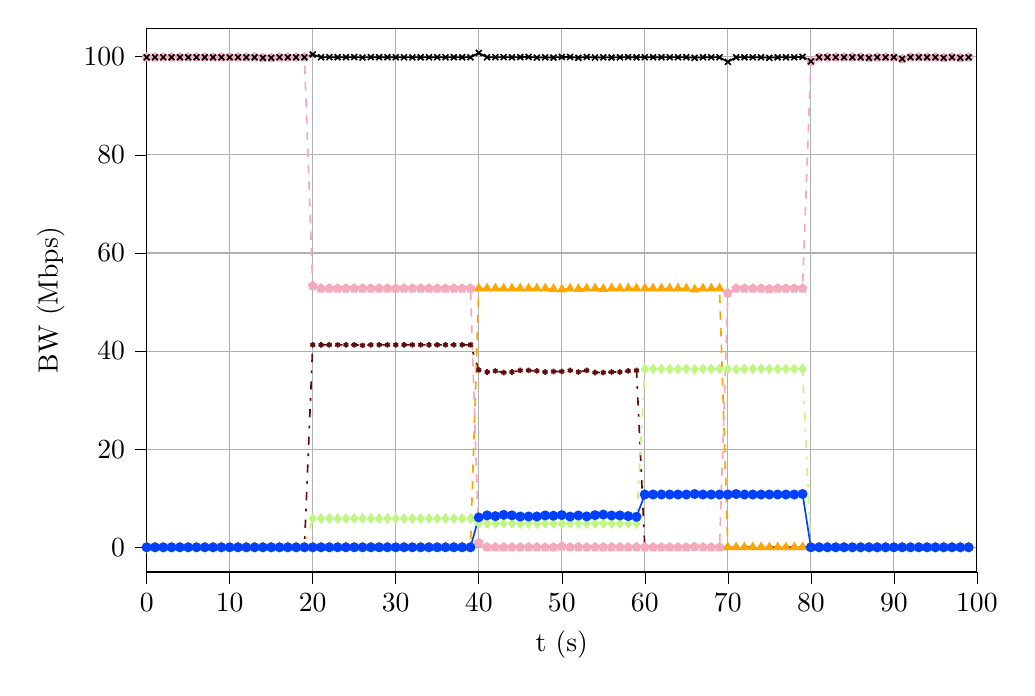
\begin{tikzpicture}

\definecolor{blue064255}{RGB}{0,64,255}
\definecolor{darkgrey176}{RGB}{176,176,176}
\definecolor{lightpink245169188}{RGB}{245,169,188}
\definecolor{maroon971111}{RGB}{97,11,11}
\definecolor{orange}{RGB}{255,165,0}
\definecolor{palegreen190247129}{RGB}{190,247,129}

\begin{axis}[
height=0.7\textwidth,
tick align=outside,
tick pos=left,
width=\textwidth,
x grid style={darkgrey176},
xlabel={t (s)},
xmajorgrids,
xmin=0, xmax=100,
xtick style={color=black},
y grid style={darkgrey176},
ylabel={BW (Mbps)},
ymajorgrids,
ymin=-5.03872622282609, ymax=105.813250679348,
ytick style={color=black}
]
\addplot [semithick, maroon971111, dash pattern=on 1pt off 3pt on 3pt off 3pt, mark=asterisk, mark size=1, mark options={solid}]
table {%
0 0
1 0
2 0
3 0
4 0
5 0
6 0
7 0
8 0
9 0
10 0
11 0
12 0
13 0
14 0
15 0
16 0
17 0
18 0
19 0
20 41.2710597826087
21 41.2710597826087
22 41.2710597826087
23 41.2710597826087
24 41.2710597826087
25 41.2710597826087
26 41.1665760869565
27 41.2710597826087
28 41.2710597826087
29 41.2710597826087
30 41.2710597826087
31 41.2710597826087
32 41.2710597826087
33 41.2710597826087
34 41.2710597826087
35 41.2710597826087
36 41.2710597826087
37 41.2710597826087
38 41.2710597826087
39 41.2710597826087
40 36.1513586956522
41 35.7334239130435
42 35.9423913043478
43 35.6289402173913
44 35.7334239130435
45 36.046875
46 36.046875
47 35.9423913043478
48 35.7334239130435
49 35.8379076086956
50 35.8379076086956
51 36.046875
52 35.7334239130435
53 36.046875
54 35.6289402173913
55 35.6289402173913
56 35.7334239130435
57 35.7334239130435
58 35.9423913043478
59 36.046875
60 0
61 0
62 0
63 0
64 0
65 0
66 0
67 0
68 0
69 0
70 0
71 0
72 0
73 0
74 0
75 0
76 0
77 0
78 0
79 0
80 0
81 0
82 0
83 0
84 0
85 0
86 0
87 0
88 0
89 0
90 0
91 0
92 0
93 0
94 0
95 0
96 0
97 0
98 0
99 0
};
\addplot [semithick, palegreen190247129, dash pattern=on 1pt off 3pt on 3pt off 3pt, mark=diamond*, mark size=1.5, mark options={solid}]
table {%
0 0
1 0
2 0
3 0
4 0
5 0
6 0
7 0
8 0
9 0
10 0
11 0
12 0
13 0
14 0
15 0
16 0
17 0
18 0
19 0
20 5.88243206521739
21 5.87198369565217
22 5.88243206521739
23 5.86153532608696
24 5.86153532608696
25 5.89288043478261
26 5.91377717391304
27 5.88243206521739
28 5.86153532608696
29 5.87198369565217
30 5.86153532608696
31 5.86153532608696
32 5.84063858695652
33 5.86153532608696
34 5.86153532608696
35 5.86153532608696
36 5.86153532608696
37 5.86153532608696
38 5.86153532608696
39 5.85108695652174
40 4.85849184782609
41 4.87938858695652
42 4.85849184782609
43 4.90028532608696
44 4.85849184782609
45 4.82714673913043
46 4.85849184782609
47 4.82714673913043
48 4.87938858695652
49 4.87938858695652
50 4.81669836956522
51 4.85849184782609
52 4.8689402173913
53 4.83759510869565
54 4.87938858695652
55 4.87938858695652
56 4.83759510869565
57 4.87938858695652
58 4.85849184782609
59 4.83759510869565
60 36.3603260869565
61 36.3603260869565
62 36.3603260869565
63 36.3603260869565
64 36.3603260869565
65 36.3603260869565
66 36.2558423913043
67 36.3603260869565
68 36.3603260869565
69 36.3603260869565
70 36.3603260869565
71 36.2558423913043
72 36.3603260869565
73 36.3603260869565
74 36.3603260869565
75 36.3603260869565
76 36.3603260869565
77 36.3603260869565
78 36.3603260869565
79 36.3603260869565
80 0
81 0
82 0
83 0
84 0
85 0
86 0
87 0
88 0
89 0
90 0
91 0
92 0
93 0
94 0
95 0
96 0
97 0
98 0
99 0
};
\addplot [semithick, orange, dashed, mark=triangle*, mark size=1.5, mark options={solid}]
table {%
0 0
1 0
2 0
3 0
4 0
5 0
6 0
7 0
8 0
9 0
10 0
11 0
12 0
13 0
14 0
15 0
16 0
17 0
18 0
19 0
20 0
21 0
22 0
23 0
24 0
25 0
26 0
27 0
28 0
29 0
30 0
31 0
32 0
33 0
34 0
35 0
36 0
37 0
38 0
39 0
40 52.7642663043478
41 52.7642663043478
42 52.7642663043478
43 52.7642663043478
44 52.7642663043478
45 52.7642663043478
46 52.7642663043478
47 52.7642663043478
48 52.7642663043478
49 52.6597826086956
50 52.5552989130435
51 52.7642663043478
52 52.6597826086956
53 52.7642663043478
54 52.7642663043478
55 52.6597826086956
56 52.7642663043478
57 52.7642663043478
58 52.7642663043478
59 52.7642663043478
60 52.7642663043478
61 52.7642663043478
62 52.7642663043478
63 52.7642663043478
64 52.7642663043478
65 52.7642663043478
66 52.5552989130435
67 52.7642663043478
68 52.7642663043478
69 52.7642663043478
70 0
71 0
72 0
73 0
74 0
75 0
76 0
77 0
78 0
79 0
80 0
81 0
82 0
83 0
84 0
85 0
86 0
87 0
88 0
89 0
90 0
91 0
92 0
93 0
94 0
95 0
96 0
97 0
98 0
99 0
};
\addplot [semithick, lightpink245169188, dashed, mark=pentagon*, mark size=1.5, mark options={solid}]
table {%
0 99.8864130434782
1 99.8864130434782
2 99.8864130434782
3 99.8864130434782
4 99.8864130434782
5 99.8864130434782
6 99.8864130434782
7 99.8864130434782
8 99.8864130434782
9 99.8864130434782
10 99.8864130434782
11 99.8864130434782
12 99.8864130434782
13 99.8864130434782
14 99.7819293478261
15 99.7819293478261
16 99.8864130434782
17 99.8864130434782
18 99.8864130434782
19 99.8864130434782
20 53.2866847826087
21 52.7642663043478
22 52.7642663043478
23 52.7642663043478
24 52.7642663043478
25 52.7642663043478
26 52.7642663043478
27 52.7642663043478
28 52.7642663043478
29 52.7642663043478
30 52.7642663043478
31 52.7642663043478
32 52.7642663043478
33 52.7642663043478
34 52.7642663043478
35 52.7642663043478
36 52.7642663043478
37 52.7642663043478
38 52.7642663043478
39 52.7642663043478
40 0.909008152173913
41 0.0114932065217391
42 0
43 0.0114932065217391
44 0.0114932065217391
45 0.0114932065217391
46 0.0114932065217391
47 0.0114932065217391
48 0
49 0.0114932065217391
50 0.183891304347826
51 0.0114932065217391
52 0.0365692934782609
53 0
54 0.0114932065217391
55 0.0365692934782609
56 0.02403125
57 0.0114932065217391
58 0
59 0.0114932065217391
60 0.0114932065217391
61 0.0114932065217391
62 0.0114932065217391
63 0.0114932065217391
64 0
65 0.0114932065217391
66 0.110752717391304
67 0.0114932065217391
68 0.0114932065217391
69 0
70 51.8239130434783
71 52.7642663043478
72 52.7642663043478
73 52.7642663043478
74 52.7642663043478
75 52.6597826086956
76 52.7642663043478
77 52.7642663043478
78 52.7642663043478
79 52.7642663043478
80 99.0505434782609
81 99.8864130434782
82 99.8864130434782
83 99.8864130434782
84 99.8864130434782
85 99.8864130434782
86 99.8864130434782
87 99.7819293478261
88 99.8864130434782
89 99.8864130434782
90 99.8864130434782
91 99.5729619565217
92 99.8864130434782
93 99.8864130434782
94 99.8864130434782
95 99.8864130434782
96 99.7819293478261
97 99.8864130434782
98 99.7819293478261
99 99.8864130434782
};
\addplot [semithick, blue064255, mark=*, mark size=1.5, mark options={solid}]
table {%
0 0
1 0
2 0
3 0
4 0
5 0
6 0
7 0
8 0
9 0
10 0
11 0
12 0
13 0
14 0
15 0
16 0
17 0
18 0
19 0
20 0
21 0
22 0
23 0
24 0
25 0
26 0
27 0
28 0
29 0
30 0
31 0
32 0
33 0
34 0
35 0
36 0
37 0
38 0
39 0
40 6.09139945652174
41 6.50933423913043
42 6.35260869565217
43 6.61381793478261
44 6.50933423913043
45 6.26902173913043
46 6.27947010869565
47 6.27947010869565
48 6.49888586956522
49 6.43619565217391
50 6.56157608695652
51 6.26902173913043
52 6.4884375
53 6.30036684782609
54 6.5511277173913
55 6.67650815217391
56 6.4884375
57 6.49888586956522
58 6.36305706521739
59 6.21677989130435
60 10.7618206521739
61 10.7618206521739
62 10.7618206521739
63 10.7618206521739
64 10.7618206521739
65 10.7618206521739
66 10.8663043478261
67 10.7618206521739
68 10.7618206521739
69 10.7618206521739
70 10.7618206521739
71 10.8663043478261
72 10.7618206521739
73 10.7618206521739
74 10.7618206521739
75 10.7618206521739
76 10.7618206521739
77 10.7618206521739
78 10.7618206521739
79 10.8663043478261
80 0
81 0
82 0
83 0
84 0
85 0
86 0
87 0
88 0
89 0
90 0
91 0
92 0
93 0
94 0
95 0
96 0
97 0
98 0
99 0
};
\addplot [semithick, black, mark=x, mark size=1.5, mark options={solid}]
table {%
0 99.8864130434782
1 99.8864130434782
2 99.8864130434782
3 99.8864130434782
4 99.8864130434782
5 99.8864130434782
6 99.8864130434782
7 99.8864130434782
8 99.8864130434782
9 99.8864130434782
10 99.8864130434782
11 99.8864130434782
12 99.8864130434782
13 99.8864130434782
14 99.7819293478261
15 99.7819293478261
16 99.8864130434782
17 99.8864130434782
18 99.8864130434782
19 99.8864130434782
20 100.440176630435
21 99.9073097826087
22 99.9177581521739
23 99.8968614130435
24 99.8968614130435
25 99.9282065217391
26 99.8446195652174
27 99.9177581521739
28 99.8968614130435
29 99.9073097826087
30 99.8968614130435
31 99.8968614130435
32 99.875964673913
33 99.8968614130435
34 99.8968614130435
35 99.8968614130435
36 99.8968614130435
37 99.8968614130435
38 99.8968614130435
39 99.8864130434783
40 100.774524456522
41 99.89790625
42 99.9177581521739
43 99.9188029891304
44 99.8770095108696
45 99.9188029891304
46 99.9605964673913
47 99.8247676630435
48 99.875964673913
49 99.8247676630434
50 99.9553722826087
51 99.9501480978261
52 99.7871535326087
53 99.9491032608695
54 99.8352160326087
55 99.8811888586957
56 99.847754076087
57 99.8874578804348
58 99.9282065217391
59 99.8770095108695
60 99.89790625
61 99.89790625
62 99.89790625
63 99.89790625
64 99.8864130434782
65 99.89790625
66 99.7881983695652
67 99.89790625
68 99.89790625
69 99.8864130434782
70 98.9460597826087
71 99.8864130434783
72 99.8864130434783
73 99.8864130434783
74 99.8864130434783
75 99.7819293478261
76 99.8864130434783
77 99.8864130434783
78 99.8864130434783
79 99.9908967391304
80 99.0505434782609
81 99.8864130434782
82 99.8864130434782
83 99.8864130434782
84 99.8864130434782
85 99.8864130434782
86 99.8864130434782
87 99.7819293478261
88 99.8864130434782
89 99.8864130434782
90 99.8864130434782
91 99.5729619565217
92 99.8864130434782
93 99.8864130434782
94 99.8864130434782
95 99.8864130434782
96 99.7819293478261
97 99.8864130434782
98 99.7819293478261
99 99.8864130434782
};
\end{axis}

\end{tikzpicture}

    \end{minipage}
    \vspace{-0.35cm}
    \caption{Bandwidth Behaviour with Table~\ref{tab:expa-params-sharing} configuration.}
    \label{other-bw-config}
\end{figure}

During \textit{Interval 1}, when only BE traffic is active, the bandwidth evolution matches that shown in Fig.~\ref{fig:expa-ietf-proposal}b. In \textit{Interval 2}, however, differences appear. Traffic classes from the \gls{tod} slice are given higher priority than those from the \gls{embb} slice. As a result, when tokens are available in the global policer, \gls{tod} slice traffic classes are prioritized for consuming the remaining bandwidth. Additionally, the \gls{tod} video traffic class is assigned a quantum value five times higher than that of the telemetry traffic class, enabling video traffic to borrow up to five times more bandwidth than telemetry traffic. Nonetheless, the \gls{cir} set for all of the traffic classes and slices is guaranteed. For instance, while BE traffic cannot borrow bandwidth due to its low priority, the \gls{cir} of the \gls{embb} slice is still respected.

During \textit{Interval 3}, all traffic classes have their \gls{cir} guaranteed. However, as shown in Table~\ref{tab:expa-params-sharing}, the \gls{urllc} and the \gls{tod} traffic classes are assigned higher priority. This ensures that any unused bandwidth is exclusively shared between these two classes according to the configured quantum values. In this scenario, since BE traffic does not have a guaranteed rate and is assigned the lowest priority, it does not consume any bandwidth, with packets from this class being denied access by the ingress policer.

In \textit{Interval 4}, the telemetry class takes over the bandwidth initially allocated to the \gls{tod} slice, while the \gls{urllc} traffic takes over the remaining available bandwidth. During the \textit{Interval 5}, when the \gls{tod} video and \gls{embb} VC traffic classes are deactivated, the active traffic flows obtain the \gls{cir} allocated to their slices, with the \gls{urllc} traffic consuming the remaining bandwidth. Finally, in \textit{Interval 6}, where only BE traffic is active in the \gls{tn}, the behavior mirrors that of \textit{Interval 1}.

The results demonstrate that, regardless of the bandwidth sharing method used, the global policer ensures that traffic is transmitted to the \gls{tn} without exceeding the global available bandwidth. This prevents packets from waiting in the \gls{drr} and priority queues of the coarse-grained resource control mechanism, while also avoiding packet losses, the same as in Figs.~\ref{fig:expa-ietf-proposal}f and \ref{fig:expa-ietf-proposal}h.

\begin{table*}
\centering
\resizebox{\textwidth}{!}{%
\begin{tabular}{cclccclccccccccll}
\cline{2-15}
\multicolumn{1}{l|}{}                                                                  & \multicolumn{10}{c|}{\cellcolor[HTML]{F5F5F5}\textbf{Fine-grained Ingress Policer Resource Control}}                                                                                                                                                                                                                                                                                                                                                                                                                                                                            & \multicolumn{4}{c|}{\cellcolor[HTML]{DAE8FC}\textbf{Coarse-grained Resource Control}}                                                                                                                                                                                                       &  &  \\ \cline{1-15}
\multicolumn{1}{|c|}{\cellcolor[HTML]{FFFFFF}}                                         & \multicolumn{4}{c|}{\cellcolor[HTML]{FFFFFF}\textbf{Class Policer}}                                                                                                                               & \multicolumn{4}{c|}{\cellcolor[HTML]{FFFFFF}\textbf{Slice Policer}}                                                                                                                                                          & \multicolumn{2}{c|}{\cellcolor[HTML]{FFFFFF}}                                                                                                & \multicolumn{4}{c|}{\cellcolor[HTML]{FFFFFF}}                                                                                                                                                                                                                                               &  &  \\ \cline{2-9}
\multicolumn{1}{|c|}{\cellcolor[HTML]{FFFFFF}}                                         & \multicolumn{2}{c|}{\cellcolor[HTML]{FFFFFF}\textbf{CIR}}           & \multicolumn{2}{c|}{\cellcolor[HTML]{FFFFFF}\textbf{PIR}}                                                                   & \multicolumn{2}{c|}{\cellcolor[HTML]{FFFFFF}\textbf{CIR}}                & \multicolumn{2}{c|}{\cellcolor[HTML]{FFFFFF}\textbf{PIR}}                                                                                         & \multicolumn{2}{c|}{\multirow{-2}{*}{\cellcolor[HTML]{FFFFFF}\textbf{Global Policer}}}                                                       & \multicolumn{4}{c|}{\multirow{-2}{*}{\cellcolor[HTML]{FFFFFF}\textbf{Quantum Parameters}}}                                                                                                                                                                                                  &  &  \\ \cline{2-15}
\multicolumn{1}{|c|}{\multirow{-3}{*}{\cellcolor[HTML]{FFFFFF}\textbf{Traffic Class}}} & \multicolumn{2}{c|}{\cellcolor[HTML]{FFFFFF}\textbf{IETF/\gls{hctns}}} & \multicolumn{1}{c|}{\cellcolor[HTML]{FFFFFF}\textbf{IETF}} & \multicolumn{1}{c|}{\cellcolor[HTML]{FFFFFF}\textbf{\gls{hctns}}} & \multicolumn{2}{c|}{\cellcolor[HTML]{FFFFFF}\textbf{IETF/\gls{hctns}}}      & \multicolumn{1}{c|}{\cellcolor[HTML]{FFFFFF}\textbf{IETF}}              & \multicolumn{1}{c|}{\cellcolor[HTML]{FFFFFF}\textbf{\gls{hctns}}}          & \multicolumn{1}{c|}{\cellcolor[HTML]{FFFFFF}\textbf{IETF}}         & \multicolumn{1}{c|}{\cellcolor[HTML]{FFFFFF}\textbf{\gls{hctns}}}          & \multicolumn{1}{c|}{\cellcolor[HTML]{FFFFFF}\textbf{Conf1}}          & \multicolumn{1}{c|}{\cellcolor[HTML]{FFFFFF}\textbf{Conf2}}           & \multicolumn{1}{c|}{\cellcolor[HTML]{FFFFFF}\textbf{Conf3}}          & \multicolumn{1}{c|}{\cellcolor[HTML]{FFFFFF}\textbf{Conf4}}           &  &  \\ \cline{1-15}
\multicolumn{1}{|c|}{\cellcolor[HTML]{FFFFFF}URLLC}                                    & \multicolumn{2}{c|}{\cellcolor[HTML]{FFFFFF}N/A}                    & \multicolumn{1}{c|}{\cellcolor[HTML]{FFFFFF}N/A}           & \multicolumn{1}{c|}{\cellcolor[HTML]{FFFFFF}N/A}               & \multicolumn{2}{c|}{\cellcolor[HTML]{FFFFFF}1.2 Mbps}                    & \multicolumn{1}{c|}{\cellcolor[HTML]{FFFFFF}100 Mbps}                   & \multicolumn{1}{c|}{\cellcolor[HTML]{FFFFFF}100 Mbps}                   & \multicolumn{1}{c|}{\cellcolor[HTML]{FFFFFF}}                      & \multicolumn{1}{c|}{\cellcolor[HTML]{FFFFFF}}                           & \multicolumn{1}{c|}{\cellcolor[HTML]{FFFFFF}PQ}                     & \multicolumn{1}{c|}{\cellcolor[HTML]{FFFFFF}PQ}                      & \multicolumn{1}{c|}{\cellcolor[HTML]{FFFFFF}PQ}                     & \multicolumn{1}{c|}{\cellcolor[HTML]{FFFFFF}PQ}                      &  &  \\ \cline{1-9} \cline{12-15}
\multicolumn{1}{|c|}{\cellcolor[HTML]{FFFFFF}Video}                                    & \multicolumn{2}{c|}{\cellcolor[HTML]{FFFFFF}32 Mbps}                & \multicolumn{1}{c|}{\cellcolor[HTML]{FFFFFF}N/A}           & \multicolumn{1}{c|}{\cellcolor[HTML]{FFFFFF}100 Mbps}          & \multicolumn{2}{c|}{\cellcolor[HTML]{FFFFFF}}                            & \multicolumn{1}{c|}{\cellcolor[HTML]{FFFFFF}}                           & \multicolumn{1}{c|}{\cellcolor[HTML]{FFFFFF}}                           & \multicolumn{1}{c|}{\cellcolor[HTML]{FFFFFF}}                      & \multicolumn{1}{c|}{\cellcolor[HTML]{FFFFFF}}                           & \multicolumn{1}{c|}{\cellcolor[HTML]{FFFFFF}1538 B}                   & \multicolumn{1}{c|}{\cellcolor[HTML]{FFFFFF}1538 B}                    & \multicolumn{1}{c|}{\cellcolor[HTML]{FFFFFF}15380 B}                  & \multicolumn{1}{c|}{\cellcolor[HTML]{FFFFFF}15380 B}                   &  &  \\ \cline{1-5} \cline{12-15}
\multicolumn{1}{|c|}{\cellcolor[HTML]{FFFFFF}Telemetry}                                & \multicolumn{2}{c|}{\cellcolor[HTML]{FFFFFF}4 Mbps}                 & \multicolumn{1}{c|}{\cellcolor[HTML]{FFFFFF}N/A}           & \multicolumn{1}{c|}{\cellcolor[HTML]{FFFFFF}100 Mbps}          & \multicolumn{2}{c|}{\multirow{-2}{*}{\cellcolor[HTML]{FFFFFF}36 Mbps}}   & \multicolumn{1}{c|}{\multirow{-2}{*}{\cellcolor[HTML]{FFFFFF}N/A}}      & \multicolumn{1}{c|}{\multirow{-2}{*}{\cellcolor[HTML]{FFFFFF}100 Mbps}} & \multicolumn{1}{c|}{\cellcolor[HTML]{FFFFFF}}                      & \multicolumn{1}{c|}{\cellcolor[HTML]{FFFFFF}}                           & \multicolumn{1}{c|}{\cellcolor[HTML]{FFFFFF}}                        & \multicolumn{1}{c|}{\cellcolor[HTML]{FFFFFF}}                         & \multicolumn{1}{c|}{\cellcolor[HTML]{FFFFFF}}                        & \multicolumn{1}{c|}{\cellcolor[HTML]{FFFFFF}}                         &  &  \\ \cline{1-9}
\multicolumn{1}{|c|}{\cellcolor[HTML]{FFFFFF}VC}                                       & \multicolumn{2}{c|}{\cellcolor[HTML]{FFFFFF}52.8 Mbps}              & \multicolumn{1}{c|}{\cellcolor[HTML]{FFFFFF}N/A}           & \multicolumn{1}{c|}{\cellcolor[HTML]{FFFFFF}100 Mbps}          & \multicolumn{2}{c|}{\cellcolor[HTML]{FFFFFF}}                            & \multicolumn{1}{c|}{\cellcolor[HTML]{FFFFFF}}                           & \multicolumn{1}{c|}{\cellcolor[HTML]{FFFFFF}}                           & \multicolumn{1}{c|}{\cellcolor[HTML]{FFFFFF}}                      & \multicolumn{1}{c|}{\cellcolor[HTML]{FFFFFF}}                           & \multicolumn{1}{c|}{\multirow{-2}{*}{\cellcolor[HTML]{FFFFFF}1538 B}} & \multicolumn{1}{c|}{\multirow{-2}{*}{\cellcolor[HTML]{FFFFFF}15380 B}} & \multicolumn{1}{c|}{\multirow{-2}{*}{\cellcolor[HTML]{FFFFFF}1538 B}} & \multicolumn{1}{c|}{\multirow{-2}{*}{\cellcolor[HTML]{FFFFFF}10766 B}} &  &  \\ \cline{1-5} \cline{12-15}
\multicolumn{1}{|c|}{\cellcolor[HTML]{FFFFFF}BE}                                       & \multicolumn{2}{c|}{\cellcolor[HTML]{FFFFFF}N/A}                    & \multicolumn{1}{c|}{\cellcolor[HTML]{FFFFFF}N/A}           & \multicolumn{1}{c|}{\cellcolor[HTML]{FFFFFF}N/A}               & \multicolumn{2}{c|}{\multirow{-2}{*}{\cellcolor[HTML]{FFFFFF}52.8 Mbps}} & \multicolumn{1}{c|}{\multirow{-2}{*}{\cellcolor[HTML]{FFFFFF}100 Mbps}} & \multicolumn{1}{c|}{\multirow{-2}{*}{\cellcolor[HTML]{FFFFFF}100 Mbps}} & \multicolumn{1}{c|}{\multirow{-5}{*}{\cellcolor[HTML]{FFFFFF}N/A}} & \multicolumn{1}{c|}{\multirow{-5}{*}{\cellcolor[HTML]{FFFFFF}100 Mbps}} & \multicolumn{1}{c|}{\cellcolor[HTML]{FFFFFF}15380 B}                  & \multicolumn{1}{c|}{\cellcolor[HTML]{FFFFFF}1538 B}                    & \multicolumn{1}{c|}{\cellcolor[HTML]{FFFFFF}1538 B}                   & \multicolumn{1}{c|}{\cellcolor[HTML]{FFFFFF}1538 B}                    &  &  \\ \cline{1-15}
\multicolumn{1}{l}{}                                                                   & \multicolumn{1}{l}{}                       &                        & \multicolumn{1}{l}{}                                       & \multicolumn{1}{l}{}                                           & \multicolumn{1}{l}{}                          &                          & \multicolumn{1}{l}{}                                                    & \multicolumn{1}{l}{}                                                    & \multicolumn{1}{l}{}                                               & \multicolumn{1}{l}{}                                                    & \multicolumn{1}{l}{}                                                 & \multicolumn{1}{l}{}                                                  & \multicolumn{1}{l}{}                                                 & \multicolumn{1}{l}{}                                                  &  &  \\
\multicolumn{1}{l}{}                                                                   & \multicolumn{1}{l}{}                       &                        & \multicolumn{1}{l}{}                                       & \multicolumn{1}{l}{}                                           & \multicolumn{1}{l}{}                          &                          & \multicolumn{1}{l}{}                                                    & \multicolumn{1}{l}{}                                                    & \multicolumn{1}{l}{}                                               & \multicolumn{1}{l}{}                                                    & \multicolumn{1}{l}{}                                                 & \multicolumn{1}{l}{}                                                  & \multicolumn{1}{l}{}                                                 & \multicolumn{1}{l}{}                                                  &  & 
\end{tabular}%
}
\vspace*{-0.25cm}
\caption{Experiment B System Parameter Configuration.}
\label{tab:expb-params}
\end{table*}

\subsubsection{Experiment B: Teleoperated Driving Slice Performance}
\label{expb}

In this experiment, we analyze the impact of coarse-grained resource control configuration on the bandwidth consumption and packet losses of the telemetry and video traffic classes within the ToD slice. The \gls{pe}1 router of our network scenario has been configured using the parameters and values listed in Table~\ref{tab:expb-params}. While the configuration of the fine-grained resource control mechanism remains unchanged, four different configurations of the coarse-grained resource control mechanism are defined in this experiment. The \gls{ietf} network slicing model and \gls{hctns} are compared. 

%% PRIMER EXPERIMENTO
\begin{figure*}[!h]
    \centering
    % LEYENDA
        \vspace*{-2.5em}
        \hspace*{-0.8cm}\includegraphics[width=1\textwidth, trim=0 10 0 10, clip]{figures/results/ExperimentB/legend_video.pdf}
    % PRIMERA FILA
    \begin{minipage}[t]{0.4\textwidth} % Primer subfigura
        \centering
        % This file was created with tikzplotlib v0.10.1.
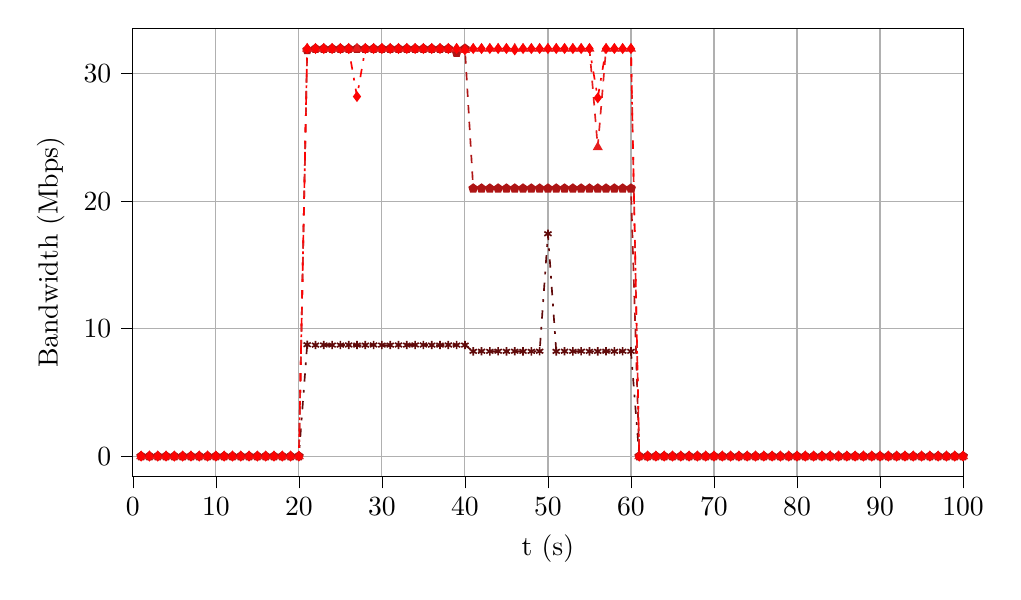
\begin{tikzpicture}

\definecolor{crimson2302929}{RGB}{230,29,29}
\definecolor{darkgrey176}{RGB}{176,176,176}
\definecolor{firebrick1742121}{RGB}{174,21,21}
\definecolor{maroon971111}{RGB}{97,11,11}
\definecolor{red25233}{RGB}{252,3,3}

\begin{axis}[
height=0.6\textwidth,
tick align=outside,
tick pos=left,
width=\textwidth,
x grid style={darkgrey176},
xlabel={t (s)},
xmajorgrids,
xmin=0, xmax=100,
xtick style={color=black},
y grid style={darkgrey176},
ylabel={Bandwidth (Mbps)},
ymajorgrids,
ymin=-1.59860054347826, ymax=33.5706114130435,
ytick style={color=black}
]
\addplot [semithick, maroon971111, dash pattern=on 1pt off 3pt on 3pt off 3pt, mark=asterisk, mark size=1.5, mark options={solid}]
table {%
1 0
2 0
3 0
4 0
5 0
6 0
7 0
8 0
9 0
10 0
11 0
12 0
13 0
14 0
15 0
16 0
17 0
18 0
19 0
20 0
21 8.74528532608696
22 8.7139402173913
23 8.72438858695652
24 8.7139402173913
25 8.7139402173913
26 8.72438858695652
27 8.7139402173913
28 8.7139402173913
29 8.72438858695652
30 8.7139402173913
31 8.7139402173913
32 8.72438858695652
33 8.7139402173913
34 8.72438858695652
35 8.72438858695652
36 8.7139402173913
37 8.7139402173913
38 8.72438858695652
39 8.7139402173913
40 8.7139402173913
41 8.22286684782609
42 8.2333152173913
43 8.22286684782609
44 8.2333152173913
45 8.22286684782609
46 8.2333152173913
47 8.22286684782609
48 8.22286684782609
49 8.2333152173913
50 17.448777173913
51 8.22286684782609
52 8.2333152173913
53 8.22286684782609
54 8.2333152173913
55 8.22286684782609
56 8.22286684782609
57 8.2333152173913
58 8.22286684782609
59 8.2333152173913
60 8.22286684782609
61 0
62 0
63 0
64 0
65 0
66 0
67 0
68 0
69 0
70 0
71 0
72 0
73 0
74 0
75 0
76 0
77 0
78 0
79 0
80 0
81 0
82 0
83 0
84 0
85 0
86 0
87 0
88 0
89 0
90 0
91 0
92 0
93 0
94 0
95 0
96 0
97 0
98 0
99 0
100 0
};
\addplot [semithick, firebrick1742121, dashed, mark=pentagon*, mark size=1.5, mark options={solid}]
table {%
1 0
2 0
3 0
4 0
5 0
6 0
7 0
8 0
9 0
10 0
11 0
12 0
13 0
14 0
15 0
16 0
17 0
18 0
19 0
20 0
21 31.867527173913
22 31.9720108695652
23 31.9720108695652
24 31.9720108695652
25 31.9720108695652
26 31.9720108695652
27 31.9720108695652
28 31.9720108695652
29 31.9720108695652
30 31.9720108695652
31 31.9720108695652
32 31.9720108695652
33 31.9720108695652
34 31.9720108695652
35 31.9720108695652
36 31.9720108695652
37 31.9720108695652
38 31.9720108695652
39 31.6585597826087
40 31.9720108695652
41 21.001222826087
42 21.001222826087
43 21.001222826087
44 21.001222826087
45 21.001222826087
46 21.001222826087
47 21.001222826087
48 21.001222826087
49 21.001222826087
50 21.001222826087
51 21.001222826087
52 21.001222826087
53 21.001222826087
54 21.001222826087
55 21.001222826087
56 21.001222826087
57 21.001222826087
58 21.001222826087
59 21.001222826087
60 21.001222826087
61 0
62 0
63 0
64 0
65 0
66 0
67 0
68 0
69 0
70 0
71 0
72 0
73 0
74 0
75 0
76 0
77 0
78 0
79 0
80 0
81 0
82 0
83 0
84 0
85 0
86 0
87 0
88 0
89 0
90 0
91 0
92 0
93 0
94 0
95 0
96 0
97 0
98 0
99 0
100 0
};
\addplot [semithick, crimson2302929, dashed, mark=triangle*, mark size=1.5, mark options={solid}]
table {%
1 0
2 0
3 0
4 0
5 0
6 0
7 0
8 0
9 0
10 0
11 0
12 0
13 0
14 0
15 0
16 0
17 0
18 0
19 0
20 0
21 31.9720108695652
22 31.9720108695652
23 31.9720108695652
24 31.9720108695652
25 31.9720108695652
26 31.9720108695652
27 31.9720108695652
28 31.9720108695652
29 31.9720108695652
30 31.9720108695652
31 31.9720108695652
32 31.9720108695652
33 31.9720108695652
34 31.9720108695652
35 31.9720108695652
36 31.9720108695652
37 31.9720108695652
38 31.9720108695652
39 31.9720108695652
40 31.867527173913
41 31.9720108695652
42 31.9720108695652
43 31.9720108695652
44 31.9720108695652
45 31.9720108695652
46 31.9720108695652
47 31.9720108695652
48 31.9720108695652
49 31.9720108695652
50 31.9720108695652
51 31.9720108695652
52 31.9720108695652
53 31.9720108695652
54 31.9720108695652
55 31.9720108695652
56 24.2402173913043
57 31.9720108695652
58 31.9720108695652
59 31.9720108695652
60 31.9720108695652
61 0
62 0
63 0
64 0
65 0
66 0
67 0
68 0
69 0
70 0
71 0
72 0
73 0
74 0
75 0
76 0
77 0
78 0
79 0
80 0
81 0
82 0
83 0
84 0
85 0
86 0
87 0
88 0
89 0
90 0
91 0
92 0
93 0
94 0
95 0
96 0
97 0
98 0
99 0
100 0
};
\addplot [semithick, red25233, dash pattern=on 1pt off 3pt on 3pt off 3pt, mark=diamond*, mark size=1.5, mark options={solid}]
table {%
1 0
2 0
3 0
4 0
5 0
6 0
7 0
8 0
9 0
10 0
11 0
12 0
13 0
14 0
15 0
16 0
17 0
18 0
19 0
20 0
21 31.9720108695652
22 31.9720108695652
23 31.9720108695652
24 31.9720108695652
25 31.9720108695652
26 31.9720108695652
27 28.210597826087
28 31.9720108695652
29 31.9720108695652
30 31.9720108695652
31 31.9720108695652
32 31.9720108695652
33 31.9720108695652
34 31.9720108695652
35 31.9720108695652
36 31.9720108695652
37 31.9720108695652
38 31.9720108695652
39 31.9720108695652
40 31.867527173913
41 31.9720108695652
42 31.9720108695652
43 31.9720108695652
44 31.9720108695652
45 31.9720108695652
46 31.867527173913
47 31.9720108695652
48 31.9720108695652
49 31.9720108695652
50 31.9720108695652
51 31.9720108695652
52 31.9720108695652
53 31.9720108695652
54 31.9720108695652
55 31.9720108695652
56 28.1061141304348
57 31.9720108695652
58 31.9720108695652
59 31.9720108695652
60 31.9720108695652
61 0
62 0
63 0
64 0
65 0
66 0
67 0
68 0
69 0
70 0
71 0
72 0
73 0
74 0
75 0
76 0
77 0
78 0
79 0
80 0
81 0
82 0
83 0
84 0
85 0
86 0
87 0
88 0
89 0
90 0
91 0
92 0
93 0
94 0
95 0
96 0
97 0
98 0
99 0
100 0
};
\end{axis}

\end{tikzpicture}
\vspace*{-0.1cm}
        \vspace*{-0.2cm} \centering \small (a) IETF: Video Bandwidth Evolution.
    \end{minipage}
    \vspace*{0.2cm}
    \hspace{1.5cm}
    \begin{minipage}[t]{0.4\textwidth} % Segunda subfigura
        \centering
        % This file was created with tikzplotlib v0.10.1.
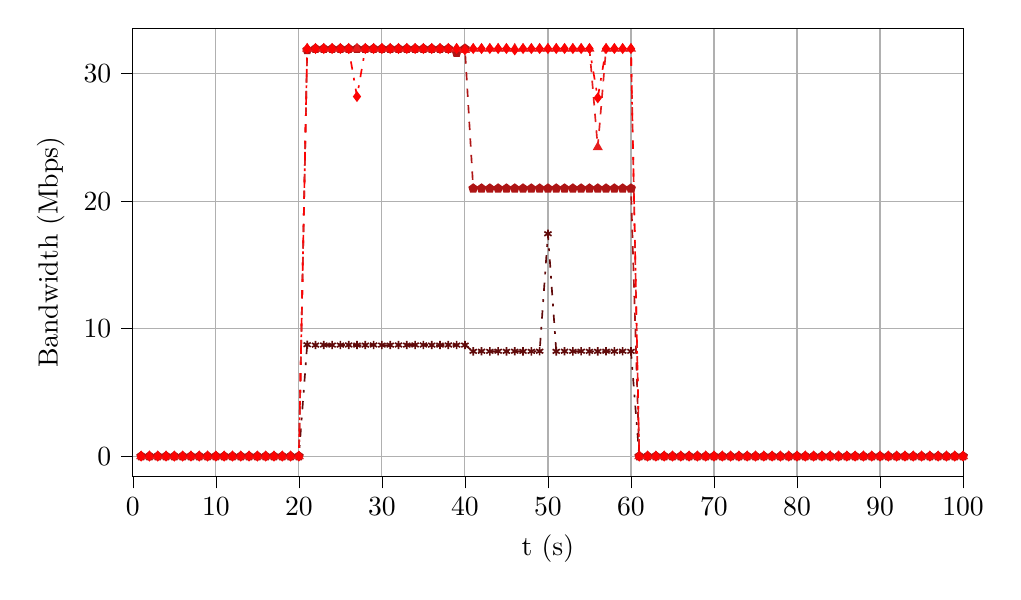
\begin{tikzpicture}

\definecolor{crimson2302929}{RGB}{230,29,29}
\definecolor{darkgrey176}{RGB}{176,176,176}
\definecolor{firebrick1742121}{RGB}{174,21,21}
\definecolor{maroon971111}{RGB}{97,11,11}
\definecolor{red25233}{RGB}{252,3,3}

\begin{axis}[
height=0.6\textwidth,
tick align=outside,
tick pos=left,
width=\textwidth,
x grid style={darkgrey176},
xlabel={t (s)},
xmajorgrids,
xmin=0, xmax=100,
xtick style={color=black},
y grid style={darkgrey176},
ylabel={Bandwidth (Mbps)},
ymajorgrids,
ymin=-1.59860054347826, ymax=33.5706114130435,
ytick style={color=black}
]
\addplot [semithick, maroon971111, dash pattern=on 1pt off 3pt on 3pt off 3pt, mark=asterisk, mark size=1.5, mark options={solid}]
table {%
1 0
2 0
3 0
4 0
5 0
6 0
7 0
8 0
9 0
10 0
11 0
12 0
13 0
14 0
15 0
16 0
17 0
18 0
19 0
20 0
21 8.74528532608696
22 8.7139402173913
23 8.72438858695652
24 8.7139402173913
25 8.7139402173913
26 8.72438858695652
27 8.7139402173913
28 8.7139402173913
29 8.72438858695652
30 8.7139402173913
31 8.7139402173913
32 8.72438858695652
33 8.7139402173913
34 8.72438858695652
35 8.72438858695652
36 8.7139402173913
37 8.7139402173913
38 8.72438858695652
39 8.7139402173913
40 8.7139402173913
41 8.22286684782609
42 8.2333152173913
43 8.22286684782609
44 8.2333152173913
45 8.22286684782609
46 8.2333152173913
47 8.22286684782609
48 8.22286684782609
49 8.2333152173913
50 17.448777173913
51 8.22286684782609
52 8.2333152173913
53 8.22286684782609
54 8.2333152173913
55 8.22286684782609
56 8.22286684782609
57 8.2333152173913
58 8.22286684782609
59 8.2333152173913
60 8.22286684782609
61 0
62 0
63 0
64 0
65 0
66 0
67 0
68 0
69 0
70 0
71 0
72 0
73 0
74 0
75 0
76 0
77 0
78 0
79 0
80 0
81 0
82 0
83 0
84 0
85 0
86 0
87 0
88 0
89 0
90 0
91 0
92 0
93 0
94 0
95 0
96 0
97 0
98 0
99 0
100 0
};
\addplot [semithick, firebrick1742121, dashed, mark=pentagon*, mark size=1.5, mark options={solid}]
table {%
1 0
2 0
3 0
4 0
5 0
6 0
7 0
8 0
9 0
10 0
11 0
12 0
13 0
14 0
15 0
16 0
17 0
18 0
19 0
20 0
21 31.867527173913
22 31.9720108695652
23 31.9720108695652
24 31.9720108695652
25 31.9720108695652
26 31.9720108695652
27 31.9720108695652
28 31.9720108695652
29 31.9720108695652
30 31.9720108695652
31 31.9720108695652
32 31.9720108695652
33 31.9720108695652
34 31.9720108695652
35 31.9720108695652
36 31.9720108695652
37 31.9720108695652
38 31.9720108695652
39 31.6585597826087
40 31.9720108695652
41 21.001222826087
42 21.001222826087
43 21.001222826087
44 21.001222826087
45 21.001222826087
46 21.001222826087
47 21.001222826087
48 21.001222826087
49 21.001222826087
50 21.001222826087
51 21.001222826087
52 21.001222826087
53 21.001222826087
54 21.001222826087
55 21.001222826087
56 21.001222826087
57 21.001222826087
58 21.001222826087
59 21.001222826087
60 21.001222826087
61 0
62 0
63 0
64 0
65 0
66 0
67 0
68 0
69 0
70 0
71 0
72 0
73 0
74 0
75 0
76 0
77 0
78 0
79 0
80 0
81 0
82 0
83 0
84 0
85 0
86 0
87 0
88 0
89 0
90 0
91 0
92 0
93 0
94 0
95 0
96 0
97 0
98 0
99 0
100 0
};
\addplot [semithick, crimson2302929, dashed, mark=triangle*, mark size=1.5, mark options={solid}]
table {%
1 0
2 0
3 0
4 0
5 0
6 0
7 0
8 0
9 0
10 0
11 0
12 0
13 0
14 0
15 0
16 0
17 0
18 0
19 0
20 0
21 31.9720108695652
22 31.9720108695652
23 31.9720108695652
24 31.9720108695652
25 31.9720108695652
26 31.9720108695652
27 31.9720108695652
28 31.9720108695652
29 31.9720108695652
30 31.9720108695652
31 31.9720108695652
32 31.9720108695652
33 31.9720108695652
34 31.9720108695652
35 31.9720108695652
36 31.9720108695652
37 31.9720108695652
38 31.9720108695652
39 31.9720108695652
40 31.867527173913
41 31.9720108695652
42 31.9720108695652
43 31.9720108695652
44 31.9720108695652
45 31.9720108695652
46 31.9720108695652
47 31.9720108695652
48 31.9720108695652
49 31.9720108695652
50 31.9720108695652
51 31.9720108695652
52 31.9720108695652
53 31.9720108695652
54 31.9720108695652
55 31.9720108695652
56 24.2402173913043
57 31.9720108695652
58 31.9720108695652
59 31.9720108695652
60 31.9720108695652
61 0
62 0
63 0
64 0
65 0
66 0
67 0
68 0
69 0
70 0
71 0
72 0
73 0
74 0
75 0
76 0
77 0
78 0
79 0
80 0
81 0
82 0
83 0
84 0
85 0
86 0
87 0
88 0
89 0
90 0
91 0
92 0
93 0
94 0
95 0
96 0
97 0
98 0
99 0
100 0
};
\addplot [semithick, red25233, dash pattern=on 1pt off 3pt on 3pt off 3pt, mark=diamond*, mark size=1.5, mark options={solid}]
table {%
1 0
2 0
3 0
4 0
5 0
6 0
7 0
8 0
9 0
10 0
11 0
12 0
13 0
14 0
15 0
16 0
17 0
18 0
19 0
20 0
21 31.9720108695652
22 31.9720108695652
23 31.9720108695652
24 31.9720108695652
25 31.9720108695652
26 31.9720108695652
27 28.210597826087
28 31.9720108695652
29 31.9720108695652
30 31.9720108695652
31 31.9720108695652
32 31.9720108695652
33 31.9720108695652
34 31.9720108695652
35 31.9720108695652
36 31.9720108695652
37 31.9720108695652
38 31.9720108695652
39 31.9720108695652
40 31.867527173913
41 31.9720108695652
42 31.9720108695652
43 31.9720108695652
44 31.9720108695652
45 31.9720108695652
46 31.867527173913
47 31.9720108695652
48 31.9720108695652
49 31.9720108695652
50 31.9720108695652
51 31.9720108695652
52 31.9720108695652
53 31.9720108695652
54 31.9720108695652
55 31.9720108695652
56 28.1061141304348
57 31.9720108695652
58 31.9720108695652
59 31.9720108695652
60 31.9720108695652
61 0
62 0
63 0
64 0
65 0
66 0
67 0
68 0
69 0
70 0
71 0
72 0
73 0
74 0
75 0
76 0
77 0
78 0
79 0
80 0
81 0
82 0
83 0
84 0
85 0
86 0
87 0
88 0
89 0
90 0
91 0
92 0
93 0
94 0
95 0
96 0
97 0
98 0
99 0
100 0
};
\end{axis}

\end{tikzpicture}

        \vspace*{-0.2cm} \centering \small (b) \gls{hctns}: Video Bandwidth Evolution.
    \end{minipage}
    \vspace*{0.2cm}

    % SEGUNDA FILA
    \begin{minipage}[t]{0.4\textwidth}
        \centering
        %
        % This file was created with tikzplotlib v0.10.1.
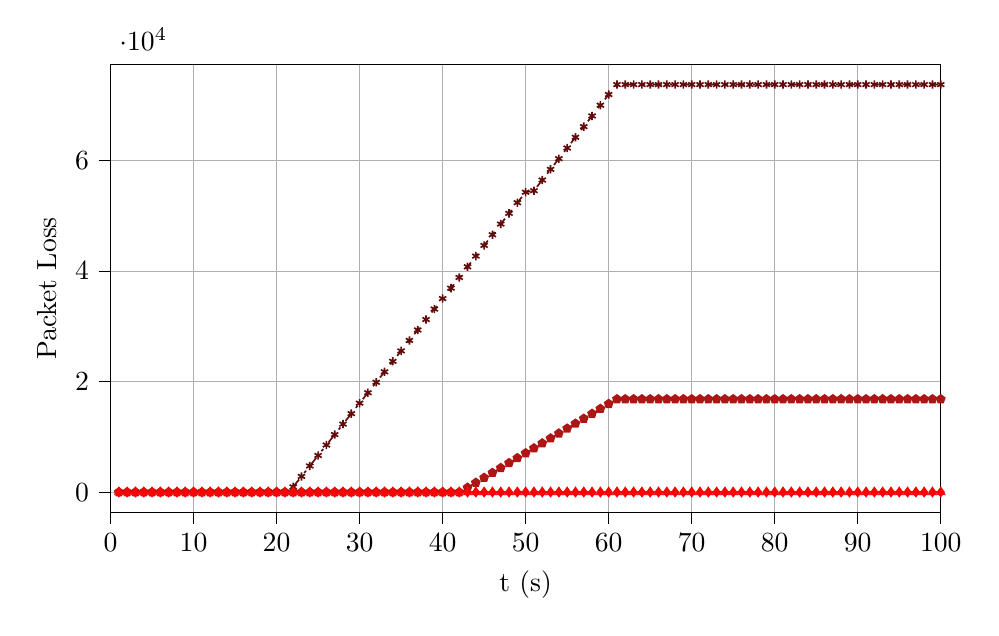
\begin{tikzpicture}

\definecolor{crimson2302929}{RGB}{230,29,29}
\definecolor{darkgrey176}{RGB}{176,176,176}
\definecolor{firebrick1742121}{RGB}{174,21,21}
\definecolor{maroon971111}{RGB}{97,11,11}
\definecolor{red25233}{RGB}{252,3,3}

\begin{axis}[
height=0.6\textwidth,
tick align=outside,
tick pos=left,
width=\textwidth,
x grid style={darkgrey176},
xlabel={t (s)},
xmajorgrids,
xmin=0, xmax=100,
xtick style={color=black},
y grid style={darkgrey176},
ylabel={Packet Loss},
ymajorgrids,
ymin=-3686.95, ymax=77425.95,
ytick style={color=black}
]
\addplot [semithick, maroon971111, dash pattern=on 1pt off 3pt on 3pt off 3pt, mark=asterisk, mark size=1.5, mark options={solid}]
table {%
1 0
2 0
3 0
4 0
5 0
6 0
7 0
8 0
9 0
10 0
11 0
12 0
13 0
14 0
15 0
16 0
17 0
18 0
19 0
20 0
21 0
22 953
23 2845
24 4740
25 6633
26 8526
27 10419
28 12311
29 14203
30 16094
31 17985
32 19877
33 21770
34 23664
35 25557
36 27450
37 29340
38 31232
39 33127
40 35020
41 36910
42 38839
43 40771
44 42706
45 44637
46 46570
47 48504
48 50438
49 52373
50 54260
51 54536
52 56470
53 58403
54 60335
55 62269
56 64203
57 66135
58 68069
59 70003
60 71938
61 73739
62 73739
63 73739
64 73739
65 73739
66 73739
67 73739
68 73739
69 73739
70 73739
71 73739
72 73739
73 73739
74 73739
75 73739
76 73739
77 73739
78 73739
79 73739
80 73739
81 73739
82 73739
83 73739
84 73739
85 73739
86 73739
87 73739
88 73739
89 73739
90 73739
91 73739
92 73739
93 73739
94 73739
95 73739
96 73739
97 73739
98 73739
99 73739
100 73739
};
\addplot [semithick, firebrick1742121, dashed, mark=pentagon*, mark size=1.5, mark options={solid}]
table {%
1 0
2 0
3 0
4 0
5 0
6 0
7 0
8 0
9 0
10 0
11 0
12 0
13 0
14 0
15 0
16 0
17 0
18 0
19 0
20 0
21 0
22 0
23 0
24 0
25 0
26 0
27 0
28 0
29 0
30 0
31 0
32 0
33 0
34 0
35 0
36 0
37 0
38 0
39 0
40 0
41 0
42 0
43 822
44 1717
45 2610
46 3499
47 4387
48 5279
49 6172
50 7064
51 7957
52 8849
53 9740
54 10632
55 11523
56 12415
57 13309
58 14195
59 15086
60 15980
61 16829
62 16829
63 16829
64 16829
65 16829
66 16829
67 16829
68 16829
69 16829
70 16829
71 16829
72 16829
73 16829
74 16829
75 16829
76 16829
77 16829
78 16829
79 16829
80 16829
81 16829
82 16829
83 16829
84 16829
85 16829
86 16829
87 16829
88 16829
89 16829
90 16829
91 16829
92 16829
93 16829
94 16829
95 16829
96 16829
97 16829
98 16829
99 16829
100 16829
};
\addplot [semithick, crimson2302929, dashed, mark=triangle*, mark size=1.5, mark options={solid}]
table {%
1 0
2 0
3 0
4 0
5 0
6 0
7 0
8 0
9 0
10 0
11 0
12 0
13 0
14 0
15 0
16 0
17 0
18 0
19 0
20 0
21 0
22 0
23 0
24 0
25 0
26 0
27 0
28 0
29 0
30 0
31 0
32 0
33 0
34 0
35 0
36 0
37 0
38 0
39 0
40 0
41 0
42 0
43 0
44 0
45 0
46 0
47 0
48 0
49 0
50 0
51 0
52 0
53 0
54 0
55 0
56 0
57 0
58 0
59 0
60 0
61 0
62 0
63 0
64 0
65 0
66 0
67 0
68 0
69 0
70 0
71 0
72 0
73 0
74 0
75 0
76 0
77 0
78 0
79 0
80 0
81 0
82 0
83 0
84 0
85 0
86 0
87 0
88 0
89 0
90 0
91 0
92 0
93 0
94 0
95 0
96 0
97 0
98 0
99 0
100 0
};
\addplot [semithick, red25233, dash pattern=on 1pt off 3pt on 3pt off 3pt, mark=diamond*, mark size=1.5, mark options={solid}]
table {%
1 0
2 0
3 0
4 0
5 0
6 0
7 0
8 0
9 0
10 0
11 0
12 0
13 0
14 0
15 0
16 0
17 0
18 0
19 0
20 0
21 0
22 0
23 0
24 0
25 0
26 0
27 0
28 0
29 0
30 0
31 0
32 0
33 0
34 0
35 0
36 0
37 0
38 0
39 0
40 0
41 0
42 0
43 0
44 0
45 0
46 0
47 0
48 0
49 0
50 0
51 0
52 0
53 0
54 0
55 0
56 0
57 0
58 0
59 0
60 0
61 0
62 0
63 0
64 0
65 0
66 0
67 0
68 0
69 0
70 0
71 0
72 0
73 0
74 0
75 0
76 0
77 0
78 0
79 0
80 0
81 0
82 0
83 0
84 0
85 0
86 0
87 0
88 0
89 0
90 0
91 0
92 0
93 0
94 0
95 0
96 0
97 0
98 0
99 0
100 0
};
\end{axis}

\end{tikzpicture}

        \vspace*{-0.2cm} \centering \small (c) IETF: Video Packet Loss in output PE port.
    \end{minipage}
    \vspace*{0.2cm}
    \hspace{1.5cm}
    \begin{minipage}[t]{0.4\textwidth} % Cuarta subfigura
        \centering
        % This file was created with tikzplotlib v0.10.1.
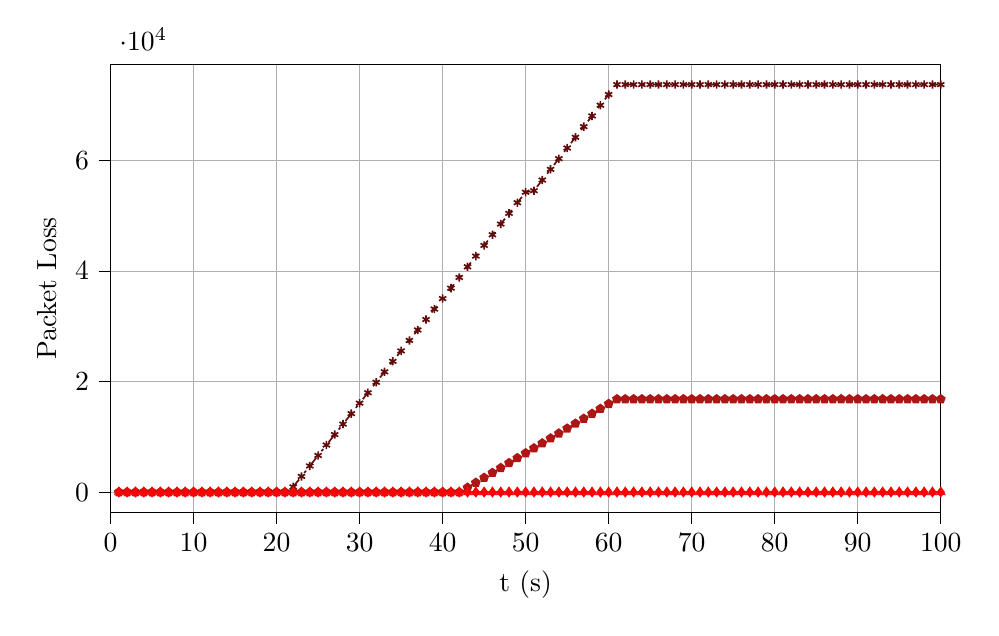
\begin{tikzpicture}

\definecolor{crimson2302929}{RGB}{230,29,29}
\definecolor{darkgrey176}{RGB}{176,176,176}
\definecolor{firebrick1742121}{RGB}{174,21,21}
\definecolor{maroon971111}{RGB}{97,11,11}
\definecolor{red25233}{RGB}{252,3,3}

\begin{axis}[
height=0.6\textwidth,
tick align=outside,
tick pos=left,
width=\textwidth,
x grid style={darkgrey176},
xlabel={t (s)},
xmajorgrids,
xmin=0, xmax=100,
xtick style={color=black},
y grid style={darkgrey176},
ylabel={Packet Loss},
ymajorgrids,
ymin=-3686.95, ymax=77425.95,
ytick style={color=black}
]
\addplot [semithick, maroon971111, dash pattern=on 1pt off 3pt on 3pt off 3pt, mark=asterisk, mark size=1.5, mark options={solid}]
table {%
1 0
2 0
3 0
4 0
5 0
6 0
7 0
8 0
9 0
10 0
11 0
12 0
13 0
14 0
15 0
16 0
17 0
18 0
19 0
20 0
21 0
22 953
23 2845
24 4740
25 6633
26 8526
27 10419
28 12311
29 14203
30 16094
31 17985
32 19877
33 21770
34 23664
35 25557
36 27450
37 29340
38 31232
39 33127
40 35020
41 36910
42 38839
43 40771
44 42706
45 44637
46 46570
47 48504
48 50438
49 52373
50 54260
51 54536
52 56470
53 58403
54 60335
55 62269
56 64203
57 66135
58 68069
59 70003
60 71938
61 73739
62 73739
63 73739
64 73739
65 73739
66 73739
67 73739
68 73739
69 73739
70 73739
71 73739
72 73739
73 73739
74 73739
75 73739
76 73739
77 73739
78 73739
79 73739
80 73739
81 73739
82 73739
83 73739
84 73739
85 73739
86 73739
87 73739
88 73739
89 73739
90 73739
91 73739
92 73739
93 73739
94 73739
95 73739
96 73739
97 73739
98 73739
99 73739
100 73739
};
\addplot [semithick, firebrick1742121, dashed, mark=pentagon*, mark size=1.5, mark options={solid}]
table {%
1 0
2 0
3 0
4 0
5 0
6 0
7 0
8 0
9 0
10 0
11 0
12 0
13 0
14 0
15 0
16 0
17 0
18 0
19 0
20 0
21 0
22 0
23 0
24 0
25 0
26 0
27 0
28 0
29 0
30 0
31 0
32 0
33 0
34 0
35 0
36 0
37 0
38 0
39 0
40 0
41 0
42 0
43 822
44 1717
45 2610
46 3499
47 4387
48 5279
49 6172
50 7064
51 7957
52 8849
53 9740
54 10632
55 11523
56 12415
57 13309
58 14195
59 15086
60 15980
61 16829
62 16829
63 16829
64 16829
65 16829
66 16829
67 16829
68 16829
69 16829
70 16829
71 16829
72 16829
73 16829
74 16829
75 16829
76 16829
77 16829
78 16829
79 16829
80 16829
81 16829
82 16829
83 16829
84 16829
85 16829
86 16829
87 16829
88 16829
89 16829
90 16829
91 16829
92 16829
93 16829
94 16829
95 16829
96 16829
97 16829
98 16829
99 16829
100 16829
};
\addplot [semithick, crimson2302929, dashed, mark=triangle*, mark size=1.5, mark options={solid}]
table {%
1 0
2 0
3 0
4 0
5 0
6 0
7 0
8 0
9 0
10 0
11 0
12 0
13 0
14 0
15 0
16 0
17 0
18 0
19 0
20 0
21 0
22 0
23 0
24 0
25 0
26 0
27 0
28 0
29 0
30 0
31 0
32 0
33 0
34 0
35 0
36 0
37 0
38 0
39 0
40 0
41 0
42 0
43 0
44 0
45 0
46 0
47 0
48 0
49 0
50 0
51 0
52 0
53 0
54 0
55 0
56 0
57 0
58 0
59 0
60 0
61 0
62 0
63 0
64 0
65 0
66 0
67 0
68 0
69 0
70 0
71 0
72 0
73 0
74 0
75 0
76 0
77 0
78 0
79 0
80 0
81 0
82 0
83 0
84 0
85 0
86 0
87 0
88 0
89 0
90 0
91 0
92 0
93 0
94 0
95 0
96 0
97 0
98 0
99 0
100 0
};
\addplot [semithick, red25233, dash pattern=on 1pt off 3pt on 3pt off 3pt, mark=diamond*, mark size=1.5, mark options={solid}]
table {%
1 0
2 0
3 0
4 0
5 0
6 0
7 0
8 0
9 0
10 0
11 0
12 0
13 0
14 0
15 0
16 0
17 0
18 0
19 0
20 0
21 0
22 0
23 0
24 0
25 0
26 0
27 0
28 0
29 0
30 0
31 0
32 0
33 0
34 0
35 0
36 0
37 0
38 0
39 0
40 0
41 0
42 0
43 0
44 0
45 0
46 0
47 0
48 0
49 0
50 0
51 0
52 0
53 0
54 0
55 0
56 0
57 0
58 0
59 0
60 0
61 0
62 0
63 0
64 0
65 0
66 0
67 0
68 0
69 0
70 0
71 0
72 0
73 0
74 0
75 0
76 0
77 0
78 0
79 0
80 0
81 0
82 0
83 0
84 0
85 0
86 0
87 0
88 0
89 0
90 0
91 0
92 0
93 0
94 0
95 0
96 0
97 0
98 0
99 0
100 0
};
\end{axis}

\end{tikzpicture}

        \vspace*{-0.2cm} \centering \small (d) \gls{hctns}: Video Packet Loss in output PE port.
    \end{minipage}
    \vspace*{0.2cm}

    % SEGUNDA LEYENDA
    \hspace*{-0.8cm}\includegraphics[width=1\textwidth, trim=0 15 0 10, clip]{figures/results/ExperimentB/legend_telemetry.pdf}
    % TERCERA FILA
    \begin{minipage}[t]{0.4\textwidth}
        \centering
        % This file was created with tikzplotlib v0.10.1.
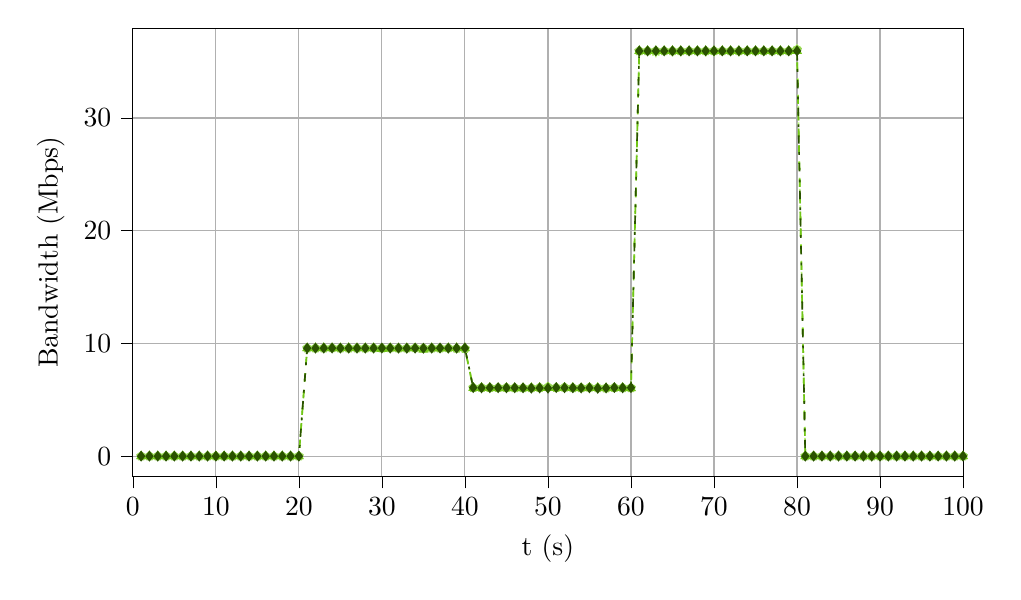
\begin{tikzpicture}

\definecolor{darkgreen42820}{RGB}{42,82,0}
\definecolor{darkgrey176}{RGB}{176,176,176}
\definecolor{palegreen190247129}{RGB}{190,247,129}
\definecolor{yellowgreen11319822}{RGB}{113,198,22}
\definecolor{yellowgreen15121484}{RGB}{151,214,84}

\begin{axis}[
height=0.6\textwidth,
tick align=outside,
tick pos=left,
width=\textwidth,
x grid style={darkgrey176},
xlabel={t (s)},
xmajorgrids,
xmin=0, xmax=100,
xtick style={color=black},
y grid style={darkgrey176},
ylabel={Bandwidth (Mbps)},
ymajorgrids,
ymin=-1.80756793478261, ymax=37.9589266304348,
ytick style={color=black}
]
\addplot [semithick, palegreen190247129, dash pattern=on 1pt off 3pt on 3pt off 3pt, mark=asterisk, mark size=1.5, mark options={solid}]
table {%
1 0
2 0
3 0
4 0
5 0
6 0
7 0
8 0
9 0
10 0
11 0
12 0
13 0
14 0
15 0
16 0
17 0
18 0
19 0
20 0
21 9.58115489130435
22 9.58115489130435
23 9.59160326086956
24 9.58115489130435
25 9.58115489130435
26 9.58115489130435
27 9.58115489130435
28 9.58115489130435
29 9.51846467391304
30 9.58115489130435
31 9.58115489130435
32 9.59160326086956
33 9.58115489130435
34 9.59160326086956
35 9.58115489130435
36 9.5498097826087
37 9.56025815217391
38 9.49756793478261
39 9.50801630434782
40 9.50801630434782
41 6.06005434782609
42 6.09139945652174
43 6.04960597826087
44 6.06005434782609
45 6.06005434782609
46 6.0705027173913
47 6.06005434782609
48 6.0705027173913
49 6.09139945652174
50 6.0705027173913
51 6.08095108695652
52 6.0705027173913
53 6.0705027173913
54 6.0705027173913
55 6.06005434782609
56 6.0705027173913
57 6.12274456521739
58 6.04960597826087
59 6.06005434782609
60 6.10184782608696
61 35.8379076086956
62 35.9423913043478
63 35.7334239130435
64 35.9423913043478
65 35.8379076086956
66 35.8379076086956
67 35.9423913043478
68 35.9423913043478
69 35.8379076086956
70 35.8379076086956
71 35.9423913043478
72 35.9423913043478
73 35.8379076086956
74 35.9423913043478
75 35.9423913043478
76 35.9423913043478
77 35.9423913043478
78 35.9423913043478
79 35.9423913043478
80 36.1513586956522
81 0
82 0
83 0
84 0
85 0
86 0
87 0
88 0
89 0
90 0
91 0
92 0
93 0
94 0
95 0
96 0
97 0
98 0
99 0
100 0
};
\addplot [semithick, yellowgreen15121484, dashed, mark=pentagon*, mark size=1.5, mark options={solid}]
table {%
1 0
2 0
3 0
4 0
5 0
6 0
7 0
8 0
9 0
10 0
11 0
12 0
13 0
14 0
15 0
16 0
17 0
18 0
19 0
20 0
21 9.58115489130435
22 9.58115489130435
23 9.58115489130435
24 9.59160326086956
25 9.58115489130435
26 9.58115489130435
27 9.58115489130435
28 9.58115489130435
29 9.59160326086956
30 9.58115489130435
31 9.59160326086956
32 9.58115489130435
33 9.57070652173913
34 9.59160326086956
35 9.58115489130435
36 9.58115489130435
37 9.58115489130435
38 9.59160326086956
39 9.5498097826087
40 9.53936141304348
41 6.0705027173913
42 6.08095108695652
43 6.0705027173913
44 6.0705027173913
45 6.08095108695652
46 6.06005434782609
47 6.04960597826087
48 6.04960597826087
49 6.08095108695652
50 6.13319293478261
51 6.08095108695652
52 6.10184782608696
53 6.06005434782609
54 6.06005434782609
55 6.09139945652174
56 6.06005434782609
57 6.02870923913043
58 6.08095108695652
59 6.06005434782609
60 6.04960597826087
61 35.9423913043478
62 35.9423913043478
63 35.9423913043478
64 35.9423913043478
65 35.9423913043478
66 35.9423913043478
67 35.9423913043478
68 35.9423913043478
69 35.9423913043478
70 35.9423913043478
71 35.9423913043478
72 35.9423913043478
73 35.9423913043478
74 35.9423913043478
75 35.9423913043478
76 35.9423913043478
77 35.9423913043478
78 35.9423913043478
79 35.9423913043478
80 36.046875
81 0
82 0
83 0
84 0
85 0
86 0
87 0
88 0
89 0
90 0
91 0
92 0
93 0
94 0
95 0
96 0
97 0
98 0
99 0
100 0
};
\addplot [semithick, yellowgreen11319822, dashed, mark=triangle*, mark size=1.5, mark options={solid}]
table {%
1 0
2 0
3 0
4 0
5 0
6 0
7 0
8 0
9 0
10 0
11 0
12 0
13 0
14 0
15 0
16 0
17 0
18 0
19 0
20 0
21 9.58115489130435
22 9.58115489130435
23 9.59160326086956
24 9.58115489130435
25 9.58115489130435
26 9.59160326086956
27 9.57070652173913
28 9.58115489130435
29 9.58115489130435
30 9.51846467391304
31 9.58115489130435
32 9.5498097826087
33 9.58115489130435
34 9.57070652173913
35 9.44532608695652
36 9.58115489130435
37 9.5498097826087
38 9.58115489130435
39 9.59160326086956
40 9.58115489130435
41 6.04960597826087
42 6.04960597826087
43 6.04960597826087
44 6.02870923913043
45 6.02870923913043
46 6.02870923913043
47 6.02870923913043
48 6.04960597826087
49 6.06005434782609
50 6.06005434782609
51 6.04960597826087
52 6.0705027173913
53 6.06005434782609
54 6.01826086956522
55 6.04960597826087
56 6.06005434782609
57 6.02870923913043
58 6.04960597826087
59 6.04960597826087
60 6.02870923913043
61 35.9423913043478
62 35.9423913043478
63 35.9423913043478
64 35.9423913043478
65 35.9423913043478
66 35.9423913043478
67 35.9423913043478
68 35.9423913043478
69 35.9423913043478
70 35.9423913043478
71 35.9423913043478
72 35.9423913043478
73 35.9423913043478
74 35.9423913043478
75 35.9423913043478
76 35.9423913043478
77 35.9423913043478
78 35.9423913043478
79 35.9423913043478
80 35.9423913043478
81 0
82 0
83 0
84 0
85 0
86 0
87 0
88 0
89 0
90 0
91 0
92 0
93 0
94 0
95 0
96 0
97 0
98 0
99 0
100 0
};
\addplot [semithick, darkgreen42820, dash pattern=on 1pt off 3pt on 3pt off 3pt, mark=diamond*, mark size=1.5, mark options={solid}]
table {%
1 0
2 0
3 0
4 0
5 0
6 0
7 0
8 0
9 0
10 0
11 0
12 0
13 0
14 0
15 0
16 0
17 0
18 0
19 0
20 0
21 9.58115489130435
22 9.58115489130435
23 9.58115489130435
24 9.59160326086956
25 9.58115489130435
26 9.58115489130435
27 9.58115489130435
28 9.58115489130435
29 9.58115489130435
30 9.59160326086956
31 9.58115489130435
32 9.58115489130435
33 9.57070652173913
34 9.58115489130435
35 9.57070652173913
36 9.58115489130435
37 9.59160326086956
38 9.58115489130435
39 9.58115489130435
40 9.59160326086956
41 6.08095108695652
42 6.06005434782609
43 6.0705027173913
44 6.0705027173913
45 6.06005434782609
46 6.0705027173913
47 6.06005434782609
48 6.02870923913043
49 6.04960597826087
50 6.02870923913043
51 6.08095108695652
52 6.0705027173913
53 6.06005434782609
54 6.04960597826087
55 6.06005434782609
56 6.01826086956522
57 6.04960597826087
58 6.08095108695652
59 6.06005434782609
60 6.08095108695652
61 35.9423913043478
62 35.9423913043478
63 35.9423913043478
64 35.9423913043478
65 35.9423913043478
66 35.9423913043478
67 35.9423913043478
68 35.9423913043478
69 35.9423913043478
70 35.9423913043478
71 35.9423913043478
72 35.9423913043478
73 35.9423913043478
74 35.9423913043478
75 35.9423913043478
76 35.9423913043478
77 35.9423913043478
78 35.9423913043478
79 35.9423913043478
80 35.9423913043478
81 0
82 0
83 0
84 0
85 0
86 0
87 0
88 0
89 0
90 0
91 0
92 0
93 0
94 0
95 0
96 0
97 0
98 0
99 0
100 0
};
\end{axis}

\end{tikzpicture}

        \centering \small (e) IETF: Telemetry Bandwidth Evolution.
    \end{minipage}
    \vspace*{0.2cm}
    \hspace{1.5cm}
    \begin{minipage}[t]{0.4\textwidth} % Cuarta subfigura
        \centering
        % This file was created with tikzplotlib v0.10.1.
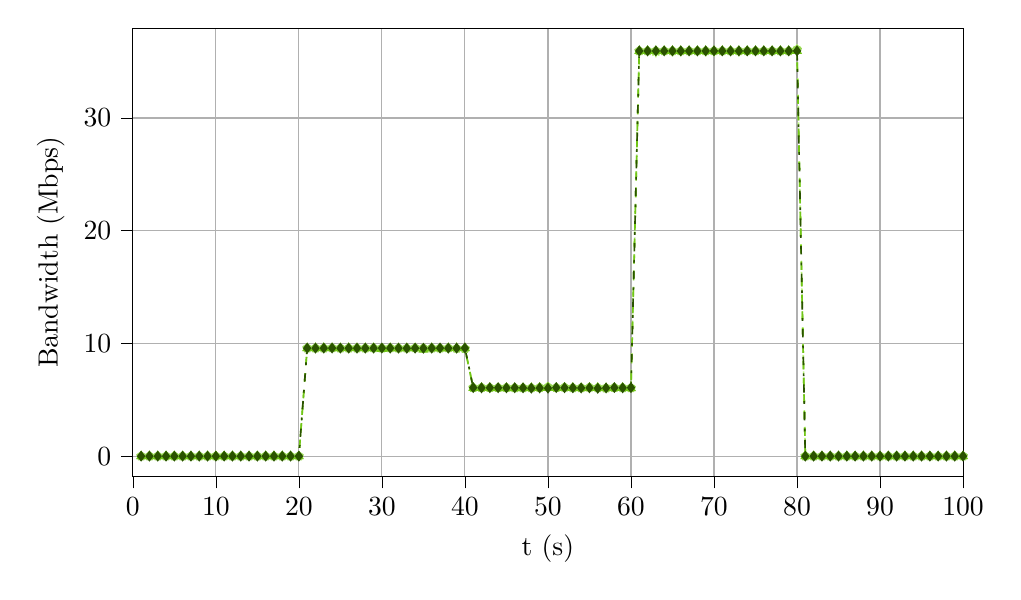
\begin{tikzpicture}

\definecolor{darkgreen42820}{RGB}{42,82,0}
\definecolor{darkgrey176}{RGB}{176,176,176}
\definecolor{palegreen190247129}{RGB}{190,247,129}
\definecolor{yellowgreen11319822}{RGB}{113,198,22}
\definecolor{yellowgreen15121484}{RGB}{151,214,84}

\begin{axis}[
height=0.6\textwidth,
tick align=outside,
tick pos=left,
width=\textwidth,
x grid style={darkgrey176},
xlabel={t (s)},
xmajorgrids,
xmin=0, xmax=100,
xtick style={color=black},
y grid style={darkgrey176},
ylabel={Bandwidth (Mbps)},
ymajorgrids,
ymin=-1.80756793478261, ymax=37.9589266304348,
ytick style={color=black}
]
\addplot [semithick, palegreen190247129, dash pattern=on 1pt off 3pt on 3pt off 3pt, mark=asterisk, mark size=1.5, mark options={solid}]
table {%
1 0
2 0
3 0
4 0
5 0
6 0
7 0
8 0
9 0
10 0
11 0
12 0
13 0
14 0
15 0
16 0
17 0
18 0
19 0
20 0
21 9.58115489130435
22 9.58115489130435
23 9.59160326086956
24 9.58115489130435
25 9.58115489130435
26 9.58115489130435
27 9.58115489130435
28 9.58115489130435
29 9.51846467391304
30 9.58115489130435
31 9.58115489130435
32 9.59160326086956
33 9.58115489130435
34 9.59160326086956
35 9.58115489130435
36 9.5498097826087
37 9.56025815217391
38 9.49756793478261
39 9.50801630434782
40 9.50801630434782
41 6.06005434782609
42 6.09139945652174
43 6.04960597826087
44 6.06005434782609
45 6.06005434782609
46 6.0705027173913
47 6.06005434782609
48 6.0705027173913
49 6.09139945652174
50 6.0705027173913
51 6.08095108695652
52 6.0705027173913
53 6.0705027173913
54 6.0705027173913
55 6.06005434782609
56 6.0705027173913
57 6.12274456521739
58 6.04960597826087
59 6.06005434782609
60 6.10184782608696
61 35.8379076086956
62 35.9423913043478
63 35.7334239130435
64 35.9423913043478
65 35.8379076086956
66 35.8379076086956
67 35.9423913043478
68 35.9423913043478
69 35.8379076086956
70 35.8379076086956
71 35.9423913043478
72 35.9423913043478
73 35.8379076086956
74 35.9423913043478
75 35.9423913043478
76 35.9423913043478
77 35.9423913043478
78 35.9423913043478
79 35.9423913043478
80 36.1513586956522
81 0
82 0
83 0
84 0
85 0
86 0
87 0
88 0
89 0
90 0
91 0
92 0
93 0
94 0
95 0
96 0
97 0
98 0
99 0
100 0
};
\addplot [semithick, yellowgreen15121484, dashed, mark=pentagon*, mark size=1.5, mark options={solid}]
table {%
1 0
2 0
3 0
4 0
5 0
6 0
7 0
8 0
9 0
10 0
11 0
12 0
13 0
14 0
15 0
16 0
17 0
18 0
19 0
20 0
21 9.58115489130435
22 9.58115489130435
23 9.58115489130435
24 9.59160326086956
25 9.58115489130435
26 9.58115489130435
27 9.58115489130435
28 9.58115489130435
29 9.59160326086956
30 9.58115489130435
31 9.59160326086956
32 9.58115489130435
33 9.57070652173913
34 9.59160326086956
35 9.58115489130435
36 9.58115489130435
37 9.58115489130435
38 9.59160326086956
39 9.5498097826087
40 9.53936141304348
41 6.0705027173913
42 6.08095108695652
43 6.0705027173913
44 6.0705027173913
45 6.08095108695652
46 6.06005434782609
47 6.04960597826087
48 6.04960597826087
49 6.08095108695652
50 6.13319293478261
51 6.08095108695652
52 6.10184782608696
53 6.06005434782609
54 6.06005434782609
55 6.09139945652174
56 6.06005434782609
57 6.02870923913043
58 6.08095108695652
59 6.06005434782609
60 6.04960597826087
61 35.9423913043478
62 35.9423913043478
63 35.9423913043478
64 35.9423913043478
65 35.9423913043478
66 35.9423913043478
67 35.9423913043478
68 35.9423913043478
69 35.9423913043478
70 35.9423913043478
71 35.9423913043478
72 35.9423913043478
73 35.9423913043478
74 35.9423913043478
75 35.9423913043478
76 35.9423913043478
77 35.9423913043478
78 35.9423913043478
79 35.9423913043478
80 36.046875
81 0
82 0
83 0
84 0
85 0
86 0
87 0
88 0
89 0
90 0
91 0
92 0
93 0
94 0
95 0
96 0
97 0
98 0
99 0
100 0
};
\addplot [semithick, yellowgreen11319822, dashed, mark=triangle*, mark size=1.5, mark options={solid}]
table {%
1 0
2 0
3 0
4 0
5 0
6 0
7 0
8 0
9 0
10 0
11 0
12 0
13 0
14 0
15 0
16 0
17 0
18 0
19 0
20 0
21 9.58115489130435
22 9.58115489130435
23 9.59160326086956
24 9.58115489130435
25 9.58115489130435
26 9.59160326086956
27 9.57070652173913
28 9.58115489130435
29 9.58115489130435
30 9.51846467391304
31 9.58115489130435
32 9.5498097826087
33 9.58115489130435
34 9.57070652173913
35 9.44532608695652
36 9.58115489130435
37 9.5498097826087
38 9.58115489130435
39 9.59160326086956
40 9.58115489130435
41 6.04960597826087
42 6.04960597826087
43 6.04960597826087
44 6.02870923913043
45 6.02870923913043
46 6.02870923913043
47 6.02870923913043
48 6.04960597826087
49 6.06005434782609
50 6.06005434782609
51 6.04960597826087
52 6.0705027173913
53 6.06005434782609
54 6.01826086956522
55 6.04960597826087
56 6.06005434782609
57 6.02870923913043
58 6.04960597826087
59 6.04960597826087
60 6.02870923913043
61 35.9423913043478
62 35.9423913043478
63 35.9423913043478
64 35.9423913043478
65 35.9423913043478
66 35.9423913043478
67 35.9423913043478
68 35.9423913043478
69 35.9423913043478
70 35.9423913043478
71 35.9423913043478
72 35.9423913043478
73 35.9423913043478
74 35.9423913043478
75 35.9423913043478
76 35.9423913043478
77 35.9423913043478
78 35.9423913043478
79 35.9423913043478
80 35.9423913043478
81 0
82 0
83 0
84 0
85 0
86 0
87 0
88 0
89 0
90 0
91 0
92 0
93 0
94 0
95 0
96 0
97 0
98 0
99 0
100 0
};
\addplot [semithick, darkgreen42820, dash pattern=on 1pt off 3pt on 3pt off 3pt, mark=diamond*, mark size=1.5, mark options={solid}]
table {%
1 0
2 0
3 0
4 0
5 0
6 0
7 0
8 0
9 0
10 0
11 0
12 0
13 0
14 0
15 0
16 0
17 0
18 0
19 0
20 0
21 9.58115489130435
22 9.58115489130435
23 9.58115489130435
24 9.59160326086956
25 9.58115489130435
26 9.58115489130435
27 9.58115489130435
28 9.58115489130435
29 9.58115489130435
30 9.59160326086956
31 9.58115489130435
32 9.58115489130435
33 9.57070652173913
34 9.58115489130435
35 9.57070652173913
36 9.58115489130435
37 9.59160326086956
38 9.58115489130435
39 9.58115489130435
40 9.59160326086956
41 6.08095108695652
42 6.06005434782609
43 6.0705027173913
44 6.0705027173913
45 6.06005434782609
46 6.0705027173913
47 6.06005434782609
48 6.02870923913043
49 6.04960597826087
50 6.02870923913043
51 6.08095108695652
52 6.0705027173913
53 6.06005434782609
54 6.04960597826087
55 6.06005434782609
56 6.01826086956522
57 6.04960597826087
58 6.08095108695652
59 6.06005434782609
60 6.08095108695652
61 35.9423913043478
62 35.9423913043478
63 35.9423913043478
64 35.9423913043478
65 35.9423913043478
66 35.9423913043478
67 35.9423913043478
68 35.9423913043478
69 35.9423913043478
70 35.9423913043478
71 35.9423913043478
72 35.9423913043478
73 35.9423913043478
74 35.9423913043478
75 35.9423913043478
76 35.9423913043478
77 35.9423913043478
78 35.9423913043478
79 35.9423913043478
80 35.9423913043478
81 0
82 0
83 0
84 0
85 0
86 0
87 0
88 0
89 0
90 0
91 0
92 0
93 0
94 0
95 0
96 0
97 0
98 0
99 0
100 0
};
\end{axis}

\end{tikzpicture}

        \centering \small (f) \gls{hctns}: Telemetry Bandwidth Evolution.
    \end{minipage}
    \vspace*{0.2cm}
    % CUARTA FILA
    \begin{minipage}[t]{0.4\textwidth}
        \centering
        % This file was created with tikzplotlib v0.10.1.
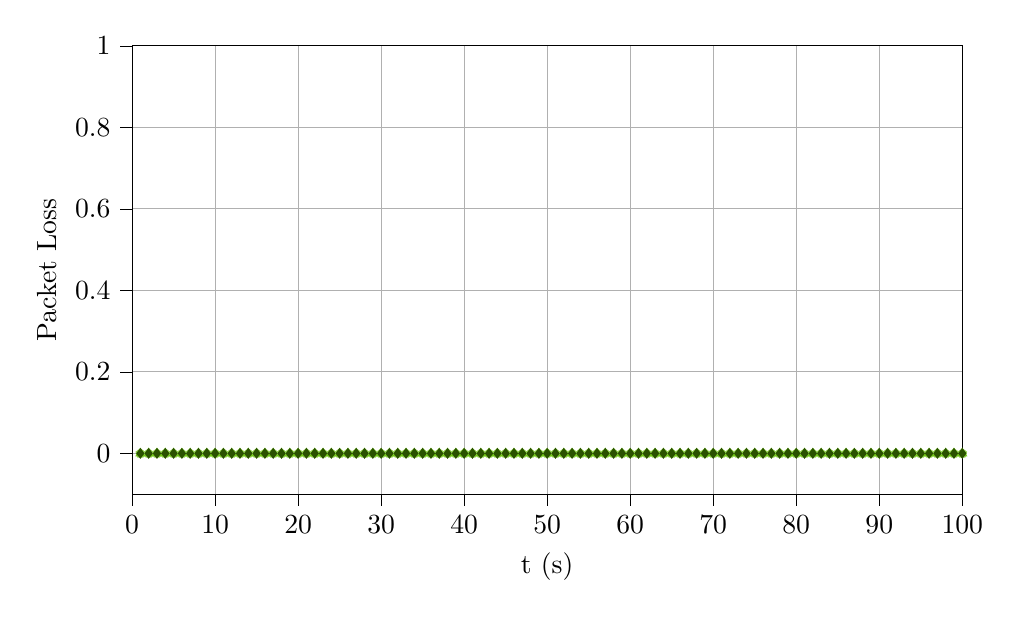
\begin{tikzpicture}

\definecolor{darkgreen42820}{RGB}{42,82,0}
\definecolor{darkgrey176}{RGB}{176,176,176}
\definecolor{palegreen190247129}{RGB}{190,247,129}
\definecolor{yellowgreen11319822}{RGB}{113,198,22}
\definecolor{yellowgreen15121484}{RGB}{151,214,84}

\begin{axis}[
height=0.6\textwidth,
tick align=outside,
tick pos=left,
width=\textwidth,
x grid style={darkgrey176},
xlabel={t (s)},
xmajorgrids,
xmin=0, xmax=100,
xtick style={color=black},
y grid style={darkgrey176},
ylabel={Packet Loss},
ymajorgrids,
ymin=-0.1, ymax=1,
ytick style={color=black}
]
\addplot [semithick, palegreen190247129, dash pattern=on 1pt off 3pt on 3pt off 3pt, mark=asterisk, mark size=1.5, mark options={solid}]
table {%
1 0
2 0
3 0
4 0
5 0
6 0
7 0
8 0
9 0
10 0
11 0
12 0
13 0
14 0
15 0
16 0
17 0
18 0
19 0
20 0
21 0
22 0
23 0
24 0
25 0
26 0
27 0
28 0
29 0
30 0
31 0
32 0
33 0
34 0
35 0
36 0
37 0
38 0
39 0
40 0
41 0
42 0
43 0
44 0
45 0
46 0
47 0
48 0
49 0
50 0
51 0
52 0
53 0
54 0
55 0
56 0
57 0
58 0
59 0
60 0
61 0
62 0
63 0
64 0
65 0
66 0
67 0
68 0
69 0
70 0
71 0
72 0
73 0
74 0
75 0
76 0
77 0
78 0
79 0
80 0
81 0
82 0
83 0
84 0
85 0
86 0
87 0
88 0
89 0
90 0
91 0
92 0
93 0
94 0
95 0
96 0
97 0
98 0
99 0
100 0
};
\addplot [semithick, yellowgreen15121484, dashed, mark=pentagon*, mark size=1.5, mark options={solid}]
table {%
1 0
2 0
3 0
4 0
5 0
6 0
7 0
8 0
9 0
10 0
11 0
12 0
13 0
14 0
15 0
16 0
17 0
18 0
19 0
20 0
21 0
22 0
23 0
24 0
25 0
26 0
27 0
28 0
29 0
30 0
31 0
32 0
33 0
34 0
35 0
36 0
37 0
38 0
39 0
40 0
41 0
42 0
43 0
44 0
45 0
46 0
47 0
48 0
49 0
50 0
51 0
52 0
53 0
54 0
55 0
56 0
57 0
58 0
59 0
60 0
61 0
62 0
63 0
64 0
65 0
66 0
67 0
68 0
69 0
70 0
71 0
72 0
73 0
74 0
75 0
76 0
77 0
78 0
79 0
80 0
81 0
82 0
83 0
84 0
85 0
86 0
87 0
88 0
89 0
90 0
91 0
92 0
93 0
94 0
95 0
96 0
97 0
98 0
99 0
100 0
};
\addplot [semithick, yellowgreen11319822, dashed, mark=triangle*, mark size=1.5, mark options={solid}]
table {%
1 0
2 0
3 0
4 0
5 0
6 0
7 0
8 0
9 0
10 0
11 0
12 0
13 0
14 0
15 0
16 0
17 0
18 0
19 0
20 0
21 0
22 0
23 0
24 0
25 0
26 0
27 0
28 0
29 0
30 0
31 0
32 0
33 0
34 0
35 0
36 0
37 0
38 0
39 0
40 0
41 0
42 0
43 0
44 0
45 0
46 0
47 0
48 0
49 0
50 0
51 0
52 0
53 0
54 0
55 0
56 0
57 0
58 0
59 0
60 0
61 0
62 0
63 0
64 0
65 0
66 0
67 0
68 0
69 0
70 0
71 0
72 0
73 0
74 0
75 0
76 0
77 0
78 0
79 0
80 0
81 0
82 0
83 0
84 0
85 0
86 0
87 0
88 0
89 0
90 0
91 0
92 0
93 0
94 0
95 0
96 0
97 0
98 0
99 0
100 0
};
\addplot [semithick, darkgreen42820, dash pattern=on 1pt off 3pt on 3pt off 3pt, mark=diamond*, mark size=1.5, mark options={solid}]
table {%
1 0
2 0
3 0
4 0
5 0
6 0
7 0
8 0
9 0
10 0
11 0
12 0
13 0
14 0
15 0
16 0
17 0
18 0
19 0
20 0
21 0
22 0
23 0
24 0
25 0
26 0
27 0
28 0
29 0
30 0
31 0
32 0
33 0
34 0
35 0
36 0
37 0
38 0
39 0
40 0
41 0
42 0
43 0
44 0
45 0
46 0
47 0
48 0
49 0
50 0
51 0
52 0
53 0
54 0
55 0
56 0
57 0
58 0
59 0
60 0
61 0
62 0
63 0
64 0
65 0
66 0
67 0
68 0
69 0
70 0
71 0
72 0
73 0
74 0
75 0
76 0
77 0
78 0
79 0
80 0
81 0
82 0
83 0
84 0
85 0
86 0
87 0
88 0
89 0
90 0
91 0
92 0
93 0
94 0
95 0
96 0
97 0
98 0
99 0
100 0
};
\end{axis}

\end{tikzpicture}

        \centering \small (g) IETF: Telemetry Packets Queued in output PE port.
    \end{minipage}
    \hspace{1.5cm}
    \begin{minipage}[t]{0.4\textwidth} % Cuarta subfigura
        \centering
        % This file was created with tikzplotlib v0.10.1.
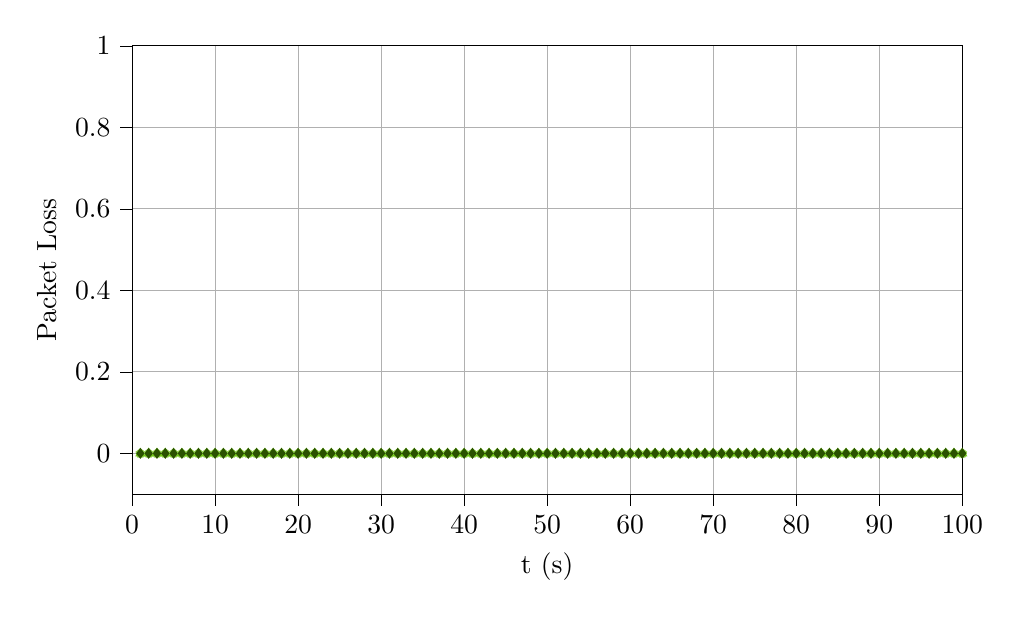
\begin{tikzpicture}

\definecolor{darkgreen42820}{RGB}{42,82,0}
\definecolor{darkgrey176}{RGB}{176,176,176}
\definecolor{palegreen190247129}{RGB}{190,247,129}
\definecolor{yellowgreen11319822}{RGB}{113,198,22}
\definecolor{yellowgreen15121484}{RGB}{151,214,84}

\begin{axis}[
height=0.6\textwidth,
tick align=outside,
tick pos=left,
width=\textwidth,
x grid style={darkgrey176},
xlabel={t (s)},
xmajorgrids,
xmin=0, xmax=100,
xtick style={color=black},
y grid style={darkgrey176},
ylabel={Packet Loss},
ymajorgrids,
ymin=-0.1, ymax=1,
ytick style={color=black}
]
\addplot [semithick, palegreen190247129, dash pattern=on 1pt off 3pt on 3pt off 3pt, mark=asterisk, mark size=1.5, mark options={solid}]
table {%
1 0
2 0
3 0
4 0
5 0
6 0
7 0
8 0
9 0
10 0
11 0
12 0
13 0
14 0
15 0
16 0
17 0
18 0
19 0
20 0
21 0
22 0
23 0
24 0
25 0
26 0
27 0
28 0
29 0
30 0
31 0
32 0
33 0
34 0
35 0
36 0
37 0
38 0
39 0
40 0
41 0
42 0
43 0
44 0
45 0
46 0
47 0
48 0
49 0
50 0
51 0
52 0
53 0
54 0
55 0
56 0
57 0
58 0
59 0
60 0
61 0
62 0
63 0
64 0
65 0
66 0
67 0
68 0
69 0
70 0
71 0
72 0
73 0
74 0
75 0
76 0
77 0
78 0
79 0
80 0
81 0
82 0
83 0
84 0
85 0
86 0
87 0
88 0
89 0
90 0
91 0
92 0
93 0
94 0
95 0
96 0
97 0
98 0
99 0
100 0
};
\addplot [semithick, yellowgreen15121484, dashed, mark=pentagon*, mark size=1.5, mark options={solid}]
table {%
1 0
2 0
3 0
4 0
5 0
6 0
7 0
8 0
9 0
10 0
11 0
12 0
13 0
14 0
15 0
16 0
17 0
18 0
19 0
20 0
21 0
22 0
23 0
24 0
25 0
26 0
27 0
28 0
29 0
30 0
31 0
32 0
33 0
34 0
35 0
36 0
37 0
38 0
39 0
40 0
41 0
42 0
43 0
44 0
45 0
46 0
47 0
48 0
49 0
50 0
51 0
52 0
53 0
54 0
55 0
56 0
57 0
58 0
59 0
60 0
61 0
62 0
63 0
64 0
65 0
66 0
67 0
68 0
69 0
70 0
71 0
72 0
73 0
74 0
75 0
76 0
77 0
78 0
79 0
80 0
81 0
82 0
83 0
84 0
85 0
86 0
87 0
88 0
89 0
90 0
91 0
92 0
93 0
94 0
95 0
96 0
97 0
98 0
99 0
100 0
};
\addplot [semithick, yellowgreen11319822, dashed, mark=triangle*, mark size=1.5, mark options={solid}]
table {%
1 0
2 0
3 0
4 0
5 0
6 0
7 0
8 0
9 0
10 0
11 0
12 0
13 0
14 0
15 0
16 0
17 0
18 0
19 0
20 0
21 0
22 0
23 0
24 0
25 0
26 0
27 0
28 0
29 0
30 0
31 0
32 0
33 0
34 0
35 0
36 0
37 0
38 0
39 0
40 0
41 0
42 0
43 0
44 0
45 0
46 0
47 0
48 0
49 0
50 0
51 0
52 0
53 0
54 0
55 0
56 0
57 0
58 0
59 0
60 0
61 0
62 0
63 0
64 0
65 0
66 0
67 0
68 0
69 0
70 0
71 0
72 0
73 0
74 0
75 0
76 0
77 0
78 0
79 0
80 0
81 0
82 0
83 0
84 0
85 0
86 0
87 0
88 0
89 0
90 0
91 0
92 0
93 0
94 0
95 0
96 0
97 0
98 0
99 0
100 0
};
\addplot [semithick, darkgreen42820, dash pattern=on 1pt off 3pt on 3pt off 3pt, mark=diamond*, mark size=1.5, mark options={solid}]
table {%
1 0
2 0
3 0
4 0
5 0
6 0
7 0
8 0
9 0
10 0
11 0
12 0
13 0
14 0
15 0
16 0
17 0
18 0
19 0
20 0
21 0
22 0
23 0
24 0
25 0
26 0
27 0
28 0
29 0
30 0
31 0
32 0
33 0
34 0
35 0
36 0
37 0
38 0
39 0
40 0
41 0
42 0
43 0
44 0
45 0
46 0
47 0
48 0
49 0
50 0
51 0
52 0
53 0
54 0
55 0
56 0
57 0
58 0
59 0
60 0
61 0
62 0
63 0
64 0
65 0
66 0
67 0
68 0
69 0
70 0
71 0
72 0
73 0
74 0
75 0
76 0
77 0
78 0
79 0
80 0
81 0
82 0
83 0
84 0
85 0
86 0
87 0
88 0
89 0
90 0
91 0
92 0
93 0
94 0
95 0
96 0
97 0
98 0
99 0
100 0
};
\end{axis}

\end{tikzpicture}

        \centering \small (h) \gls{hctns}: Telemetry Packets Queued in output PE port.
    \end{minipage}
    \vspace*{0.1cm}
    \caption{Experiment B: \gls{ietf} versus our proposed network slicing model.}
    \label{expb-ietf-proposal}
\end{figure*}

This experiment also spans 100\,s and it is divided into the same six time intervals defined for Experiment A. First, we analyze the performance of the \gls{ietf} model. As illustrated in Fig.~\ref{expb-ietf-proposal}a, with the third and fourth coarse-grained configurations, the \gls{tod} video traffic flow achieves its guaranteed rate throughout the entire experiment. In contrast, with the first two configurations, this guarantee is not met due to packet losses occurring at the output port of \gls{pe}1, as shown in Fig.~\ref{expb-ietf-proposal}c. This is caused by the low quantum value assigned to the queue of the \gls{tn} \gls{qos} class B (i.e., the \gls{tn} \gls{qos} class assigned to video) in the first two configurations. This quantum is significantly lower than the values assigned to the other \gls{drr} queues, resulting in a reduced transmission rate at the output port for the \gls{tn} \gls{qos} class B queue. Consequently, when there is traffic in the other \gls{drr} queues, more packets arrive in the \gls{drr} queue associated with \gls{tn} \gls{qos} class B than can be transmitted, leading to an accumulation of packets, overflow of the queue, and packet losses.

For telemetry traffic, with the \gls{ietf} model, as shown in Fig.~\ref{expb-ietf-proposal}e, with the second and fourth coarse-grained configurations, the telemetry traffic achieves its guaranteed rate throughout the entire experiment. However, with the first and third configurations, this guarantee is not met due to packet losses occurring at the output port of \gls{pe}1, as shown in Fig.~\ref{expb-ietf-proposal}g. The same reasons given in the previous point apply to this case. The quantum values set in the second and fourth configurations favor the transmission of the \gls{tn} \gls{qos} class C (i.e., the \gls{tn} \gls{qos} class associated to telemetry). 

These results highlight the importance of properly configuring the coarse-grained resource control parameters in transport network routers when employing the \gls{ietf} network slicing model. In contrast, the slice model proposed in this paper guarantees bandwidth levels for both video and telemetry traffic (Figs.~\ref{expb-ietf-proposal}b and~\ref{expb-ietf-proposal}f), while preventing packet losses (Figs.~\ref{expb-ietf-proposal}d and~\ref{expb-ietf-proposal}h). This is particularly crucial for a service like \gls{tod}, which demands high-reliable communications with guaranteed bandwidth to ensure road safety. \gls{hctns} demonstrates robustness and independence from the coarse-grained resource control configuration under normal traffic conditions (without traffic bursts), ensuring that traffic classes receive the \gls{qos} level they require. Experiment C illustrates how the proposed traffic burst control mechanism performs under different network scenarios.

\subsubsection{Experiment C: Traffic Burst Control}

This experiment analyzes the impact of traffic bursts on the latency experienced by packets from different traffic classes and slices. The \gls{ietf} model does not incorporate this function, so results only show the performance of \rev{the \cite{Lin2021} model and} our proposed traffic control burst mechanism for \gls{hctns}. For this purpose, the \gls{pe}1 router of our network scenario has been configured using the parameters and values listed in Table~\ref{tab:expc-params}. Unlike Experiment A, the fine-grained resource control mechanism in this experiment incorporates traffic burst control, with the \gls{cbs} and the \gls{pbs} parameters defined for both models. \rev{Although the work in~\cite{Lin2021} does not address traffic burst control, it mentions that the \gls{trtcm} mechanism they use has two parameters, \gls{cbs} and \gls{pbs}, that can be used to control traffic bursts. For Experiment C, we have configured these parameters in our implementation of the~\cite{Lin2021} model.  Table~\ref{tab:expc-params} shows some differences between the \gls{cir} and \gls{pir} parameters configured for \gls{hctns} and the~\cite{Lin2021} model. To make the closest comparison between the two models, since \gls{hctns} treats all the traffic accepted with the same \gls{qos}, we have configured the burst in \cite{Lin2021} using only the \gls{cbs} parameter, in order to treat all burst traffic as ``green". The \gls{pbs} values remain at their default setting, i.e, the maximum packet size. As   Table~\ref{tab:expc-params} shows, the \gls{cbs} and \gls{pbs} parameters have not been specified for BE traffic, which means that the bucket sizes can only store enough tokens to allow the transmission of a single packet. This is because BE traffic does not have a guaranteed rate.} Additionally, Table~\ref{tab:expc-params} indicates that two coarse-grained resource control configurations have been applied in our model to analyze how traffic burst control behaves under these two configurations. \rev{In \cite{Lin2021}, only two priority queues are used, so no other parameter configurations are possible.}

\begin{table*}
\centering
\resizebox{\textwidth}{!}{%
\begin{tabular}{ccccccccccccccccc}
\cline{2-17}
\multicolumn{1}{c|}{}                                                                  & \multicolumn{13}{c|}{\cellcolor[HTML]{F5F5F5}\textbf{Fine-grained Ingress Policer Resource Control}}                                                                                                                                                                                                                                                                                                                                                                                                                                                                                                                                                                                                                                                                                                                                                                                  & \multicolumn{3}{c|}{\cellcolor[HTML]{DAE8FC}\textbf{\begin{tabular}[c]{@{}c@{}}Coarse-grained \\ Resource Control\end{tabular}}}                                                                                                                                                                                                   \\ \cline{2-17} 
\multicolumn{1}{c|}{}                                                                  & \multicolumn{9}{c|}{\cellcolor[HTML]{FFFFFF}\textbf{HCTNS}}                                                                                                                                                                                                                                                                                                                                                                                                                                                                                                                                                                           & \multicolumn{4}{c|}{\cellcolor[HTML]{FFFFFF}}                                                                                                                                                                                                 & \multicolumn{3}{c|}{\cellcolor[HTML]{FFFFFF}\textbf{\begin{tabular}[c]{@{}c@{}}TN QoS Class\\ Parameters\end{tabular}}}                                                                                                                                                                \\ \cline{1-10} \cline{15-17} 
\rowcolor[HTML]{FFFFFF} 
\multicolumn{1}{|c|}{\cellcolor[HTML]{FFFFFF}}                                         & \multicolumn{4}{c|}{\cellcolor[HTML]{FFFFFF}\textbf{Class Policer}}                                                                                                                                                                           & \multicolumn{4}{c|}{\cellcolor[HTML]{FFFFFF}\textbf{Slice Policer}}                                                                                                                                                                                                                          & \multicolumn{1}{c|}{\cellcolor[HTML]{FFFFFF}}                                          & \multicolumn{4}{c|}{\multirow{-2}{*}{\cellcolor[HTML]{FFFFFF}\textbf{trTCM} \cite{Lin2021}}}                                                                                                                                 & \multicolumn{2}{c|}{\cellcolor[HTML]{FFFFFF}\textbf{HCTNS}}                                                                                  & \multicolumn{1}{c|}{\cellcolor[HTML]{FFFFFF} \cite{Lin2021}}                                                            \\ \cline{2-9} \cline{11-17} 
\rowcolor[HTML]{FFFFFF} 
\multicolumn{1}{|c|}{\multirow{-2}{*}{\cellcolor[HTML]{FFFFFF}\textbf{\begin{tabular}[c]{@{}c@{}}Traffic\\ Class\end{tabular}}}} & \multicolumn{1}{c|}{\cellcolor[HTML]{FFFFFF}\textbf{CIR}} & \multicolumn{1}{c|}{\cellcolor[HTML]{FFFFFF}\textbf{PIR}} & \multicolumn{1}{c|}{\cellcolor[HTML]{FFFFFF}\textbf{CBS}} & \multicolumn{1}{c|}{\cellcolor[HTML]{FFFFFF}\textbf{PBS}} & \multicolumn{1}{c|}{\cellcolor[HTML]{FFFFFF}\textbf{CIR}}                & \multicolumn{1}{c|}{\cellcolor[HTML]{FFFFFF}\textbf{PIR}}               & \multicolumn{1}{c|}{\cellcolor[HTML]{FFFFFF}\textbf{CBS}}          & \multicolumn{1}{c|}{\cellcolor[HTML]{FFFFFF}\textbf{PBS}}          & \multicolumn{1}{c|}{\multirow{-2}{*}{\cellcolor[HTML]{FFFFFF}\textbf{\begin{tabular}[c]{@{}c@{}}Global\\ Policer\end{tabular}}}} & \multicolumn{1}{c|}{\cellcolor[HTML]{FFFFFF}\textbf{CIR}} & \multicolumn{1}{c|}{\cellcolor[HTML]{FFFFFF}\textbf{PIR}} & \multicolumn{1}{c|}{\cellcolor[HTML]{FFFFFF}\textbf{CBS}} & \multicolumn{1}{c|}{\cellcolor[HTML]{FFFFFF}\textbf{PBS}} & \multicolumn{1}{c|}{\cellcolor[HTML]{FFFFFF}\textbf{Conf1}}          & \multicolumn{1}{c|}{\cellcolor[HTML]{FFFFFF}\textbf{Conf2}}           & \multicolumn{1}{c|}{\cellcolor[HTML]{FFFFFF}}                                                                                           \\ \cline{1-16}
\rowcolor[HTML]{FFFFFF} 
\multicolumn{1}{|c|}{\cellcolor[HTML]{FFFFFF}URLLC}                                    & \multicolumn{1}{c|}{\cellcolor[HTML]{FFFFFF}N/A}          & \multicolumn{1}{c|}{\cellcolor[HTML]{FFFFFF}N/A}          & \multicolumn{1}{c|}{\cellcolor[HTML]{FFFFFF}N/A}          & \multicolumn{1}{c|}{\cellcolor[HTML]{FFFFFF}N/A}          & \multicolumn{1}{c|}{\cellcolor[HTML]{FFFFFF}1.2 Mbps}                    & \multicolumn{1}{c|}{\cellcolor[HTML]{FFFFFF}100 Mbps}                   & \multicolumn{1}{c|}{\cellcolor[HTML]{FFFFFF}50 KB}                 & \multicolumn{1}{c|}{\cellcolor[HTML]{FFFFFF}50 KB}                 & \multicolumn{1}{c|}{\cellcolor[HTML]{FFFFFF}}                                          & \multicolumn{1}{c|}{\cellcolor[HTML]{FFFFFF}1.2 Mbps}     & \multicolumn{1}{c|}{\cellcolor[HTML]{FFFFFF}100 Mbps}     & \multicolumn{1}{c|}{\cellcolor[HTML]{FFFFFF}50 KB}        & \multicolumn{1}{c|}{\cellcolor[HTML]{FFFFFF}1538 B}        & \multicolumn{1}{c|}{\cellcolor[HTML]{FFFFFF}PQ}                     & \multicolumn{1}{c|}{\cellcolor[HTML]{FFFFFF}PQ}                      & \multicolumn{1}{c|}{\cellcolor[HTML]{FFFFFF}}                                                                                           \\ \cline{1-9} \cline{11-16}
\rowcolor[HTML]{FFFFFF} 
\multicolumn{1}{|c|}{\cellcolor[HTML]{FFFFFF}Video}                                    & \multicolumn{1}{c|}{\cellcolor[HTML]{FFFFFF}32 Mbps}      & \multicolumn{1}{c|}{\cellcolor[HTML]{FFFFFF}100 Mbps}     & \multicolumn{1}{c|}{\cellcolor[HTML]{FFFFFF}50 KB}        & \multicolumn{1}{c|}{\cellcolor[HTML]{FFFFFF}50 KB}        & \multicolumn{1}{c|}{\cellcolor[HTML]{FFFFFF}}                            & \multicolumn{1}{c|}{\cellcolor[HTML]{FFFFFF}}                           & \multicolumn{1}{c|}{\cellcolor[HTML]{FFFFFF}}                      & \multicolumn{1}{c|}{\cellcolor[HTML]{FFFFFF}}                      & \multicolumn{1}{c|}{\cellcolor[HTML]{FFFFFF}}                                          & \multicolumn{1}{c|}{\cellcolor[HTML]{FFFFFF}32 Mbps}      & \multicolumn{1}{c|}{\cellcolor[HTML]{FFFFFF}100 Mbps}     & \multicolumn{1}{c|}{\cellcolor[HTML]{FFFFFF}50 KB}        & \multicolumn{1}{c|}{\cellcolor[HTML]{FFFFFF}1538 B}        & \multicolumn{1}{c|}{\cellcolor[HTML]{FFFFFF}1538 B}                   & \multicolumn{1}{c|}{\cellcolor[HTML]{FFFFFF}15380 B}                   & \multicolumn{1}{c|}{\cellcolor[HTML]{FFFFFF}}                                                                                           \\ \cline{1-5} \cline{11-16}
\rowcolor[HTML]{FFFFFF} 
\multicolumn{1}{|c|}{\cellcolor[HTML]{FFFFFF}Telemetry}                                & \multicolumn{1}{c|}{\cellcolor[HTML]{FFFFFF}4 Mbps}       & \multicolumn{1}{c|}{\cellcolor[HTML]{FFFFFF}100 Mbps}     & \multicolumn{1}{c|}{\cellcolor[HTML]{FFFFFF}50 KB}        & \multicolumn{1}{c|}{\cellcolor[HTML]{FFFFFF}50 KB}        & \multicolumn{1}{c|}{\multirow{-2}{*}{\cellcolor[HTML]{FFFFFF}36 Mbps}}   & \multicolumn{1}{c|}{\multirow{-2}{*}{\cellcolor[HTML]{FFFFFF}100 Mbps}} & \multicolumn{1}{c|}{\multirow{-2}{*}{\cellcolor[HTML]{FFFFFF}1538 B}} & \multicolumn{1}{c|}{\multirow{-2}{*}{\cellcolor[HTML]{FFFFFF}1538 B}} & \multicolumn{1}{c|}{\cellcolor[HTML]{FFFFFF}}                                          & \multicolumn{1}{c|}{\cellcolor[HTML]{FFFFFF}4 Mbps}       & \multicolumn{1}{c|}{\cellcolor[HTML]{FFFFFF}100 Mbps}     & \multicolumn{1}{c|}{\cellcolor[HTML]{FFFFFF}50 KB}        & \multicolumn{1}{c|}{\cellcolor[HTML]{FFFFFF}1538 B}        & \multicolumn{1}{c|}{\cellcolor[HTML]{FFFFFF}}                        & \multicolumn{1}{c|}{\cellcolor[HTML]{FFFFFF}}                         & \multicolumn{1}{c|}{\cellcolor[HTML]{FFFFFF}}                                                                                           \\ \cline{1-9} \cline{11-14}
\rowcolor[HTML]{FFFFFF} 
\multicolumn{1}{|c|}{\cellcolor[HTML]{FFFFFF}VC}                                       & \multicolumn{1}{c|}{\cellcolor[HTML]{FFFFFF}52.8 Mbps}    & \multicolumn{1}{c|}{\cellcolor[HTML]{FFFFFF}100 Mbps}     & \multicolumn{1}{c|}{\cellcolor[HTML]{FFFFFF}50 KB}        & \multicolumn{1}{c|}{\cellcolor[HTML]{FFFFFF}50 KB}        & \multicolumn{1}{c|}{\cellcolor[HTML]{FFFFFF}}                            & \multicolumn{1}{c|}{\cellcolor[HTML]{FFFFFF}}                           & \multicolumn{1}{c|}{\cellcolor[HTML]{FFFFFF}}                      & \multicolumn{1}{c|}{\cellcolor[HTML]{FFFFFF}}                      & \multicolumn{1}{c|}{\cellcolor[HTML]{FFFFFF}}                                          & \multicolumn{1}{c|}{\cellcolor[HTML]{FFFFFF}52.8 Mbps}    & \multicolumn{1}{c|}{\cellcolor[HTML]{FFFFFF}100 Mbps}     & \multicolumn{1}{c|}{\cellcolor[HTML]{FFFFFF}50 KB}        & \multicolumn{1}{c|}{\cellcolor[HTML]{FFFFFF}1538 B}        & \multicolumn{1}{c|}{\multirow{-2}{*}{\cellcolor[HTML]{FFFFFF}1538 B}} & \multicolumn{1}{c|}{\multirow{-2}{*}{\cellcolor[HTML]{FFFFFF}10766 B}} & \multicolumn{1}{c|}{\cellcolor[HTML]{FFFFFF}}                                                                                           \\ \cline{1-5} \cline{11-16}
\rowcolor[HTML]{FFFFFF} 
\multicolumn{1}{|c|}{\cellcolor[HTML]{FFFFFF}BE}                                       & \multicolumn{1}{c|}{\cellcolor[HTML]{FFFFFF}N/A}          & \multicolumn{1}{c|}{\cellcolor[HTML]{FFFFFF}N/A}          & \multicolumn{1}{c|}{\cellcolor[HTML]{FFFFFF}N/A}          & \multicolumn{1}{c|}{\cellcolor[HTML]{FFFFFF}N/A}          & \multicolumn{1}{c|}{\multirow{-2}{*}{\cellcolor[HTML]{FFFFFF}52.8 Mbps}} & \multicolumn{1}{c|}{\multirow{-2}{*}{\cellcolor[HTML]{FFFFFF}100 Mbps}} & \multicolumn{1}{c|}{\multirow{-2}{*}{\cellcolor[HTML]{FFFFFF}1538 B}} & \multicolumn{1}{c|}{\multirow{-2}{*}{\cellcolor[HTML]{FFFFFF}1538 B}} & \multicolumn{1}{c|}{\multirow{-5}{*}{\cellcolor[HTML]{FFFFFF}100 Mbps}}                & \multicolumn{1}{c|}{\cellcolor[HTML]{FFFFFF}N/A}          & \multicolumn{1}{c|}{\cellcolor[HTML]{FFFFFF}100 Mbps}     & \multicolumn{1}{c|}{\cellcolor[HTML]{FFFFFF}N/A}        & \multicolumn{1}{c|}{\cellcolor[HTML]{FFFFFF}1538 B}        & \multicolumn{1}{c|}{\cellcolor[HTML]{FFFFFF}1538 B}                   & \multicolumn{1}{c|}{\cellcolor[HTML]{FFFFFF}1538 B}                    & \multicolumn{1}{c|}{\multirow{-6}{*}{\cellcolor[HTML]{FFFFFF}\begin{tabular}[c]{@{}c@{}}A: HPQ \\ B: LPQ \end{tabular}}} \\ \hline
\multicolumn{1}{l}{}                                                                   & \multicolumn{1}{l}{}                                      & \multicolumn{1}{l}{}                                      & \multicolumn{1}{l}{}                                      & \multicolumn{1}{l}{}                                      & \multicolumn{1}{l}{}                                                     & \multicolumn{1}{l}{}                                                    & \multicolumn{1}{l}{}                                               & \multicolumn{1}{l}{}                                               & \multicolumn{1}{l}{}                                                                   & \multicolumn{1}{l}{}                                      & \multicolumn{1}{l}{}                                      & \multicolumn{1}{l}{}                                      & \multicolumn{1}{l}{}                                      & \multicolumn{1}{l}{}                                                 & \multicolumn{1}{l}{}                                                  & \multicolumn{1}{l}{}                                                                                                                    \\
\multicolumn{1}{l}{}                                                                   & \multicolumn{1}{l}{}                                      & \multicolumn{1}{l}{}                                      & \multicolumn{1}{l}{}                                      & \multicolumn{1}{l}{}                                      & \multicolumn{1}{l}{}                                                     & \multicolumn{1}{l}{}                                                    & \multicolumn{1}{l}{}                                               & \multicolumn{1}{l}{}                                               & \multicolumn{1}{l}{}                                                                   & \multicolumn{1}{l}{}                                      & \multicolumn{1}{l}{}                                      & \multicolumn{1}{l}{}                                      & \multicolumn{1}{l}{}                                      & \multicolumn{1}{l}{}                                                 & \multicolumn{1}{l}{}                                                  & \multicolumn{1}{l}{}                                                                                                                    \\
\multicolumn{1}{l}{}                                                                   & \multicolumn{1}{l}{}                                      & \multicolumn{1}{l}{}                                      & \multicolumn{1}{l}{}                                      & \multicolumn{1}{l}{}                                      & \multicolumn{1}{l}{}                                                     & \multicolumn{1}{l}{}                                                    & \multicolumn{1}{l}{}                                               & \multicolumn{1}{l}{}                                               & \multicolumn{1}{l}{}                                                                   & \multicolumn{1}{l}{}                                      & \multicolumn{1}{l}{}                                      & \multicolumn{1}{l}{}                                      & \multicolumn{1}{l}{}                                      & \multicolumn{1}{l}{}                                                 & \multicolumn{1}{l}{}                                                  & \multicolumn{1}{l}{}                                                                                                                   
\end{tabular}%
}
\vspace*{-0.45cm}
\caption{Experiment C System Parameter Configuration}
\label{tab:expc-params}
\end{table*}   

This experiment lasts 60 seconds and is divided into the three following time intervals: 

\begin{enumerate}
    \item Interval 1 (from \( t = 0 \, \text{s} \) to \( t = 10 \, \text{s} \)): All traffic classes are active, but there are no traffic bursts during this interval. 
    \item Interval 2 (from \( t = 10 \, \text{s} \) to \( t = 45 \, \text{s} \)): All traffic classes are active and transmitting at a constant rate. However, traffic bursts are introduced for all classes: \gls{urllc} generates a burst every second, the \gls{tod} video every two seconds, and both \gls{tod} telemetry and \gls{embb} VC every five seconds.
    \item Interval 3 (from \( t = 45 \, \text{s} \) to \( t = 60 \, \text{s} \)): the same conditions as Interval 2, except that the traffic burst from \gls{urllc} is no longer present.
\end{enumerate}

\rev{All flows have a background constant rate that is significantly below their guaranteed rate, except for BE traffic, which is transmitted at 100\,Mbps. This approach ensures that the buckets have time to refill, allowing multiple bursts per class to be observed rather than just one. Moreover, throughout the experiment, all generated bursts have a uniform size of 100\,KB. The traffic generated for this experiment is shown in Fig. \ref{expc-conf}a.}

The results are presented in Figs.~\ref{expc-conf}b, \ref{expc-conf}c, \ref{expc-conf}d and \ref{expc-conf}e, illustrating  the \gls{qos} achieved by the traffic flows in terms of both bandwidth and latency with both models. The \textit{Conf1} configuration shown in Table~\ref{tab:expc-params} for the coarse-grained resource control has been used in the \gls{hctns} model to obtain these results.

\afterpage{
\begin{figure*}[!h]
    \vspace*{-2em}
    \centering
    \includegraphics[width=1\textwidth, trim=50 10 50 10, clip]{figures/results/ExperimentA/legend_5g.pdf}
    \begin{minipage}[t]{0.45\textwidth} % Primer subfigura
        \centering
        % This file was created with tikzplotlib v0.10.1.
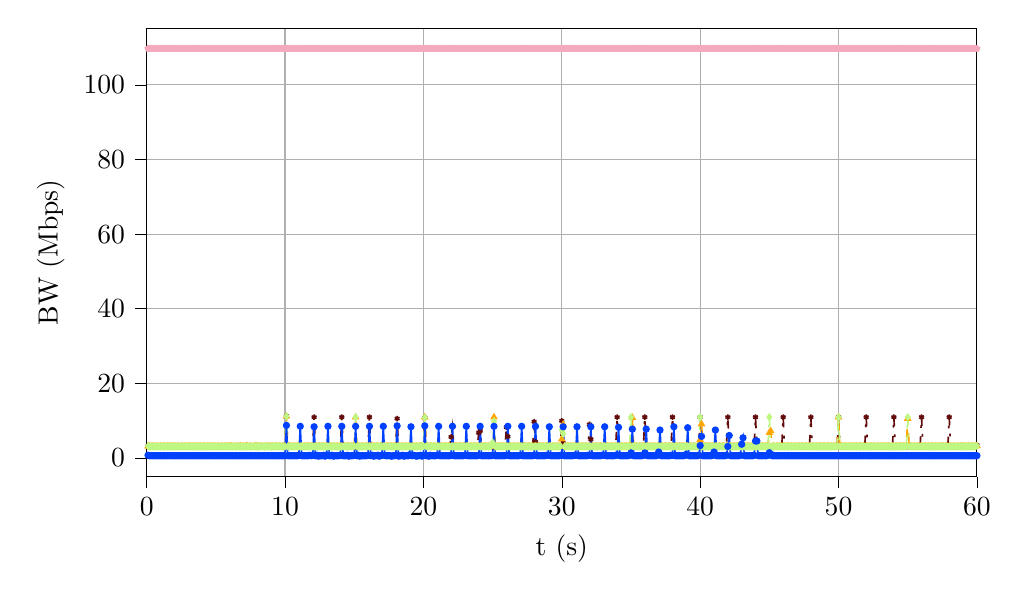
\begin{tikzpicture}

\definecolor{blue064255}{RGB}{0,64,255}
\definecolor{darkgrey176}{RGB}{176,176,176}
\definecolor{lightpink245169188}{RGB}{245,169,188}
\definecolor{maroon971111}{RGB}{97,11,11}
\definecolor{orange}{RGB}{255,165,0}
\definecolor{palegreen190247129}{RGB}{190,247,129}

\begin{axis}[
height=0.6\textwidth,
tick align=outside,
tick pos=left,
width=\textwidth,
x grid style={darkgrey176},
xlabel={t (s)},
xmajorgrids,
xmin=0, xmax=60,
xtick style={color=black},
y grid style={darkgrey176},
ylabel={BW (Mbps)},
ymajorgrids,
ymin=-4.9686699048913, ymax=115.168668546196,
ytick style={color=black}
]
\addplot [semithick, maroon971111, dash pattern=on 1pt off 3pt on 3pt off 3pt, mark=asterisk, mark size=1, mark options={solid}]
table {%
0.1 3.19720108695652
0.2 3.07182065217391
0.3 3.07182065217391
0.4 3.07182065217391
0.5 3.07182065217391
0.6 3.07182065217391
0.7 3.07182065217391
0.8 3.07182065217391
0.9 3.07182065217391
1 3.07182065217391
1.1 3.07182065217391
1.2 3.07182065217391
1.3 3.07182065217391
1.4 3.07182065217391
1.5 3.07182065217391
1.6 3.07182065217391
1.7 3.07182065217391
1.8 3.07182065217391
1.9 3.07182065217391
2 3.07182065217391
2.1 3.07182065217391
2.2 3.07182065217391
2.3 3.07182065217391
2.4 3.07182065217391
2.5 3.07182065217391
2.6 3.07182065217391
2.7 3.07182065217391
2.8 3.07182065217391
2.9 3.07182065217391
3 3.07182065217391
3.1 3.07182065217391
3.2 3.07182065217391
3.3 3.07182065217391
3.4 3.07182065217391
3.5 3.07182065217391
3.6 3.07182065217391
3.7 3.07182065217391
3.8 3.07182065217391
3.9 3.07182065217391
4 3.07182065217391
4.1 3.07182065217391
4.2 3.07182065217391
4.3 3.07182065217391
4.4 3.07182065217391
4.5 3.07182065217391
4.6 3.07182065217391
4.7 3.07182065217391
4.8 3.07182065217391
4.9 3.07182065217391
5 3.07182065217391
5.1 3.07182065217391
5.2 3.07182065217391
5.3 3.07182065217391
5.4 3.07182065217391
5.5 3.07182065217391
5.6 3.07182065217391
5.7 3.07182065217391
5.8 3.07182065217391
5.9 3.07182065217391
6 3.07182065217391
6.1 3.07182065217391
6.2 3.07182065217391
6.3 3.07182065217391
6.4 3.07182065217391
6.5 3.07182065217391
6.6 3.07182065217391
6.7 3.07182065217391
6.8 3.07182065217391
6.9 3.07182065217391
7 3.07182065217391
7.1 3.07182065217391
7.2 3.07182065217391
7.3 3.07182065217391
7.4 3.07182065217391
7.5 3.07182065217391
7.6 3.07182065217391
7.7 3.07182065217391
7.8 3.07182065217391
7.9 3.07182065217391
8 3.07182065217391
8.1 3.07182065217391
8.2 3.07182065217391
8.3 3.07182065217391
8.4 3.07182065217391
8.5 3.07182065217391
8.6 3.07182065217391
8.7 3.07182065217391
8.8 3.07182065217391
8.9 3.07182065217391
9 3.07182065217391
9.1 3.07182065217391
9.2 3.07182065217391
9.3 3.07182065217391
9.4 3.19720108695652
9.5 3.07182065217391
9.6 3.07182065217391
9.7 3.07182065217391
9.8 3.07182065217391
9.9 3.07182065217391
10 3.07182065217391
10.1 11.1902038043478
10.2 3.07182065217391
10.3 3.07182065217391
10.4 3.07182065217391
10.5 3.07182065217391
10.6 3.07182065217391
10.7 3.07182065217391
10.8 3.07182065217391
10.9 3.07182065217391
11 3.07182065217391
11.1 3.07182065217391
11.2 3.07182065217391
11.3 3.07182065217391
11.4 3.07182065217391
11.5 3.07182065217391
11.6 3.07182065217391
11.7 3.07182065217391
11.8 3.07182065217391
11.9 3.07182065217391
12 3.19511141304348
12.1 10.9498913043478
12.2 3.07182065217391
12.3 3.07182065217391
12.4 3.07182065217391
12.5 3.07182065217391
12.6 3.07182065217391
12.7 3.07182065217391
12.8 3.07182065217391
12.9 3.07182065217391
13 3.07182065217391
13.1 3.07182065217391
13.2 3.07182065217391
13.3 3.07182065217391
13.4 3.07182065217391
13.5 3.07182065217391
13.6 3.07182065217391
13.7 3.07182065217391
13.8 3.07182065217391
13.9 3.07182065217391
14 3.19511141304348
14.1 10.9498913043478
14.2 3.07182065217391
14.3 3.07182065217391
14.4 3.07182065217391
14.5 3.07182065217391
14.6 3.07182065217391
14.7 3.07182065217391
14.8 3.07182065217391
14.9 3.07182065217391
15 3.07182065217391
15.1 3.07182065217391
15.2 3.07182065217391
15.3 3.07182065217391
15.4 3.07182065217391
15.5 3.07182065217391
15.6 3.07182065217391
15.7 3.07182065217391
15.8 3.07182065217391
15.9 3.07182065217391
16 3.19511141304348
16.1 10.9498913043478
16.2 3.07182065217391
16.3 3.07182065217391
16.4 3.07182065217391
16.5 3.07182065217391
16.6 3.07182065217391
16.7 3.07182065217391
16.8 3.07182065217391
16.9 3.07182065217391
17 3.07182065217391
17.1 3.07182065217391
17.2 3.07182065217391
17.3 3.07182065217391
17.4 3.07182065217391
17.5 3.07182065217391
17.6 3.07182065217391
17.7 3.07182065217391
17.8 3.07182065217391
17.9 3.19511141304348
18 3.44064809782609
18.1 10.57375
18.2 3.07182065217391
18.3 3.07182065217391
18.4 3.07182065217391
18.5 3.07182065217391
18.6 3.07182065217391
18.7 3.07182065217391
18.8 3.07182065217391
18.9 3.07182065217391
19 3.07182065217391
19.1 3.07182065217391
19.2 3.07182065217391
19.3 3.07182065217391
19.4 3.07182065217391
19.5 3.07182065217391
19.6 3.07182065217391
19.7 3.07182065217391
19.8 3.07182065217391
19.9 3.19511141304348
20 3.19511141304348
20.1 10.8245108695652
20.2 3.07182065217391
20.3 3.07182065217391
20.4 3.07182065217391
20.5 3.07182065217391
20.6 3.07182065217391
20.7 3.07182065217391
20.8 3.07182065217391
20.9 3.07182065217391
21 3.07182065217391
21.1 3.07182065217391
21.2 3.07182065217391
21.3 3.07182065217391
21.4 3.07182065217391
21.5 3.07182065217391
21.6 3.07182065217391
21.7 3.07182065217391
21.8 3.07182065217391
21.9 3.19511141304348
22 5.65256793478261
22.1 8.35869565217391
22.2 3.07182065217391
22.3 3.07182065217391
22.4 3.07182065217391
22.5 3.07182065217391
22.6 3.07182065217391
22.7 3.07182065217391
22.8 3.07182065217391
22.9 3.07182065217391
23 3.07182065217391
23.1 3.07182065217391
23.2 3.07182065217391
23.3 3.07182065217391
23.4 3.07182065217391
23.5 3.07182065217391
23.6 3.07182065217391
23.7 3.07182065217391
23.8 3.07182065217391
23.9 3.19511141304348
24 6.76009510869565
24.1 7.25116847826087
24.2 3.07182065217391
24.3 3.07182065217391
24.4 3.07182065217391
24.5 3.07182065217391
24.6 3.07182065217391
24.7 3.07182065217391
24.8 3.07182065217391
24.9 3.07182065217391
25 3.07182065217391
25.1 3.07182065217391
25.2 3.07182065217391
25.3 3.07182065217391
25.4 3.07182065217391
25.5 3.07182065217391
25.6 3.07182065217391
25.7 3.07182065217391
25.8 3.07182065217391
25.9 3.19511141304348
26 8.24376358695652
26.1 5.77794836956522
26.2 3.07182065217391
26.3 3.07182065217391
26.4 3.07182065217391
26.5 3.07182065217391
26.6 3.07182065217391
26.7 3.07182065217391
26.8 3.07182065217391
26.9 3.07182065217391
27 3.07182065217391
27.1 3.07182065217391
27.2 3.07182065217391
27.3 3.07182065217391
27.4 3.07182065217391
27.5 3.07182065217391
27.6 3.07182065217391
27.7 3.07182065217391
27.8 3.07182065217391
27.9 3.19511141304348
28 9.71698369565217
28.1 4.30472826086956
28.2 3.07182065217391
28.3 3.07182065217391
28.4 3.07182065217391
28.5 3.07182065217391
28.6 3.07182065217391
28.7 3.07182065217391
28.8 3.07182065217391
28.9 3.07182065217391
29 3.07182065217391
29.1 3.07182065217391
29.2 3.07182065217391
29.3 3.07182065217391
29.4 3.07182065217391
29.5 3.07182065217391
29.6 3.07182065217391
29.7 3.07182065217391
29.8 3.07182065217391
29.9 3.19511141304348
30 9.95729619565217
30.1 4.05605706521739
30.2 3.07182065217391
30.3 3.07182065217391
30.4 3.07182065217391
30.5 3.07182065217391
30.6 3.07182065217391
30.7 3.07182065217391
30.8 3.07182065217391
30.9 3.07182065217391
31 3.07182065217391
31.1 3.07182065217391
31.2 3.07182065217391
31.3 3.07182065217391
31.4 3.07182065217391
31.5 3.07182065217391
31.6 3.07182065217391
31.7 3.07182065217391
31.8 3.07182065217391
31.9 3.19511141304348
32 8.97514945652174
32.1 5.03611413043478
32.2 3.07182065217391
32.3 3.07182065217391
32.4 3.07182065217391
32.5 3.07182065217391
32.6 3.07182065217391
32.7 3.07182065217391
32.8 3.07182065217391
32.9 3.07182065217391
33 3.07182065217391
33.1 3.07182065217391
33.2 3.07182065217391
33.3 3.07182065217391
33.4 3.07182065217391
33.5 3.07182065217391
33.6 3.07182065217391
33.7 3.07182065217391
33.8 3.07182065217391
33.9 3.19511141304348
34 10.9498913043478
34.1 3.07182065217391
34.2 3.07182065217391
34.3 3.07182065217391
34.4 3.07182065217391
34.5 3.07182065217391
34.6 3.07182065217391
34.7 3.07182065217391
34.8 3.07182065217391
34.9 3.07182065217391
35 3.07182065217391
35.1 3.07182065217391
35.2 3.07182065217391
35.3 3.07182065217391
35.4 3.07182065217391
35.5 3.07182065217391
35.6 3.07182065217391
35.7 3.07182065217391
35.8 3.07182065217391
35.9 3.19511141304348
36 10.9498913043478
36.1 3.07182065217391
36.2 3.07182065217391
36.3 3.07182065217391
36.4 3.07182065217391
36.5 3.07182065217391
36.6 3.07182065217391
36.7 3.07182065217391
36.8 3.07182065217391
36.9 3.07182065217391
37 3.07182065217391
37.1 3.07182065217391
37.2 3.07182065217391
37.3 3.07182065217391
37.4 3.07182065217391
37.5 3.07182065217391
37.6 3.07182065217391
37.7 3.07182065217391
37.8 3.07182065217391
37.9 3.19511141304348
38 10.9498913043478
38.1 3.07182065217391
38.2 3.07182065217391
38.3 3.07182065217391
38.4 3.07182065217391
38.5 3.07182065217391
38.6 3.07182065217391
38.7 3.07182065217391
38.8 3.07182065217391
38.9 3.07182065217391
39 3.07182065217391
39.1 3.07182065217391
39.2 3.07182065217391
39.3 3.07182065217391
39.4 3.07182065217391
39.5 3.07182065217391
39.6 3.07182065217391
39.7 3.07182065217391
39.8 3.07182065217391
39.9 3.19511141304348
40 10.9498913043478
40.1 3.07182065217391
40.2 3.07182065217391
40.3 3.07182065217391
40.4 3.07182065217391
40.5 3.07182065217391
40.6 3.07182065217391
40.7 3.07182065217391
40.8 3.07182065217391
40.9 3.07182065217391
41 3.07182065217391
41.1 3.07182065217391
41.2 3.07182065217391
41.3 3.07182065217391
41.4 3.07182065217391
41.5 3.07182065217391
41.6 3.07182065217391
41.7 3.07182065217391
41.8 3.07182065217391
41.9 3.19511141304348
42 10.9498913043478
42.1 3.07182065217391
42.2 3.07182065217391
42.3 3.07182065217391
42.4 3.07182065217391
42.5 3.07182065217391
42.6 3.07182065217391
42.7 3.07182065217391
42.8 3.07182065217391
42.9 3.07182065217391
43 3.07182065217391
43.1 3.07182065217391
43.2 3.07182065217391
43.3 3.07182065217391
43.4 3.07182065217391
43.5 3.07182065217391
43.6 3.07182065217391
43.7 3.07182065217391
43.8 3.07182065217391
43.9 3.19511141304348
44 10.9498913043478
44.1 3.07182065217391
44.2 3.07182065217391
44.3 3.07182065217391
44.4 3.07182065217391
44.5 3.07182065217391
44.6 3.07182065217391
44.7 3.07182065217391
44.8 3.07182065217391
44.9 3.07182065217391
45 3.07182065217391
45.1 3.07182065217391
45.2 3.07182065217391
45.3 2.95688858695652
45.4 3.19720108695652
45.5 3.07182065217391
45.6 3.07182065217391
45.7 3.07182065217391
45.8 3.07182065217391
45.9 3.19511141304348
46 10.9498913043478
46.1 3.07182065217391
46.2 3.07182065217391
46.3 3.07182065217391
46.4 3.07182065217391
46.5 3.07182065217391
46.6 3.07182065217391
46.7 3.07182065217391
46.8 3.07182065217391
46.9 3.07182065217391
47 3.07182065217391
47.1 3.07182065217391
47.2 3.07182065217391
47.3 3.07182065217391
47.4 3.07182065217391
47.5 3.07182065217391
47.6 3.07182065217391
47.7 3.07182065217391
47.8 3.07182065217391
47.9 3.19511141304348
48 10.9498913043478
48.1 3.07182065217391
48.2 3.07182065217391
48.3 3.07182065217391
48.4 3.07182065217391
48.5 3.07182065217391
48.6 3.07182065217391
48.7 3.07182065217391
48.8 3.07182065217391
48.9 3.07182065217391
49 3.07182065217391
49.1 3.07182065217391
49.2 3.07182065217391
49.3 3.07182065217391
49.4 3.07182065217391
49.5 3.07182065217391
49.6 3.07182065217391
49.7 3.07182065217391
49.8 3.07182065217391
49.9 3.19511141304348
50 10.9498913043478
50.1 3.07182065217391
50.2 3.07182065217391
50.3 3.07182065217391
50.4 3.07182065217391
50.5 3.07182065217391
50.6 3.07182065217391
50.7 3.07182065217391
50.8 3.07182065217391
50.9 3.07182065217391
51 3.07182065217391
51.1 3.07182065217391
51.2 3.07182065217391
51.3 3.07182065217391
51.4 3.07182065217391
51.5 3.07182065217391
51.6 3.07182065217391
51.7 3.07182065217391
51.8 3.07182065217391
51.9 3.19511141304348
52 10.9498913043478
52.1 3.07182065217391
52.2 3.07182065217391
52.3 3.07182065217391
52.4 3.07182065217391
52.5 3.07182065217391
52.6 3.07182065217391
52.7 3.07182065217391
52.8 3.07182065217391
52.9 3.07182065217391
53 3.07182065217391
53.1 3.07182065217391
53.2 3.07182065217391
53.3 3.07182065217391
53.4 3.07182065217391
53.5 3.07182065217391
53.6 3.07182065217391
53.7 3.07182065217391
53.8 3.07182065217391
53.9 3.19511141304348
54 10.9498913043478
54.1 3.07182065217391
54.2 3.07182065217391
54.3 3.07182065217391
54.4 3.07182065217391
54.5 3.07182065217391
54.6 3.07182065217391
54.7 3.07182065217391
54.8 3.07182065217391
54.9 3.07182065217391
55 3.07182065217391
55.1 3.07182065217391
55.2 3.07182065217391
55.3 3.07182065217391
55.4 3.07182065217391
55.5 3.07182065217391
55.6 3.07182065217391
55.7 3.07182065217391
55.8 3.07182065217391
55.9 3.19511141304348
56 10.9498913043478
56.1 3.07182065217391
56.2 3.07182065217391
56.3 3.07182065217391
56.4 3.07182065217391
56.5 3.07182065217391
56.6 3.07182065217391
56.7 3.07182065217391
56.8 3.07182065217391
56.9 3.07182065217391
57 3.07182065217391
57.1 3.07182065217391
57.2 3.07182065217391
57.3 3.07182065217391
57.4 3.07182065217391
57.5 3.07182065217391
57.6 3.07182065217391
57.7 3.07182065217391
57.8 3.07182065217391
57.9 3.19511141304348
58 10.9498913043478
58.1 3.07182065217391
58.2 3.07182065217391
58.3 3.07182065217391
58.4 3.07182065217391
58.5 3.07182065217391
58.6 3.07182065217391
58.7 3.07182065217391
58.8 3.07182065217391
58.9 3.07182065217391
59 3.07182065217391
59.1 3.07182065217391
59.2 3.07182065217391
59.3 3.07182065217391
59.4 3.07182065217391
59.5 3.07182065217391
59.6 3.07182065217391
59.7 3.07182065217391
59.8 3.07182065217391
59.9 3.19511141304348
60 3.47199320652174
};
\addplot [semithick, lightpink245169188, dashed, mark=pentagon*, mark size=1, mark options={solid}]
table {%
0.1 109.707880434783
0.2 109.707880434783
0.3 109.707880434783
0.4 109.707880434783
0.5 109.707880434783
0.6 109.707880434783
0.7 109.707880434783
0.8 109.707880434783
0.9 109.707880434783
1 109.707880434783
1.1 109.707880434783
1.2 109.707880434783
1.3 109.707880434783
1.4 109.707880434783
1.5 109.707880434783
1.6 109.707880434783
1.7 109.707880434783
1.8 109.707880434783
1.9 109.707880434783
2 109.707880434783
2.1 109.707880434783
2.2 109.707880434783
2.3 109.707880434783
2.4 109.707880434783
2.5 109.707880434783
2.6 109.707880434783
2.7 109.707880434783
2.8 109.707880434783
2.9 109.707880434783
3 109.707880434783
3.1 109.707880434783
3.2 109.707880434783
3.3 109.707880434783
3.4 109.707880434783
3.5 109.707880434783
3.6 109.707880434783
3.7 109.707880434783
3.8 109.707880434783
3.9 109.707880434783
4 109.707880434783
4.1 109.707880434783
4.2 109.707880434783
4.3 109.707880434783
4.4 109.707880434783
4.5 109.707880434783
4.6 109.707880434783
4.7 109.707880434783
4.8 109.707880434783
4.9 109.707880434783
5 109.707880434783
5.1 109.707880434783
5.2 109.707880434783
5.3 109.707880434783
5.4 109.707880434783
5.5 109.707880434783
5.6 109.707880434783
5.7 109.707880434783
5.8 109.707880434783
5.9 109.707880434783
6 109.707880434783
6.1 109.707880434783
6.2 109.707880434783
6.3 109.707880434783
6.4 109.707880434783
6.5 109.707880434783
6.6 109.707880434783
6.7 109.707880434783
6.8 109.707880434783
6.9 109.707880434783
7 109.707880434783
7.1 109.707880434783
7.2 109.707880434783
7.3 109.707880434783
7.4 109.707880434783
7.5 109.707880434783
7.6 109.707880434783
7.7 109.707880434783
7.8 109.707880434783
7.9 109.707880434783
8 109.707880434783
8.1 109.707880434783
8.2 109.707880434783
8.3 109.707880434783
8.4 109.707880434783
8.5 109.707880434783
8.6 109.707880434783
8.7 109.707880434783
8.8 109.707880434783
8.9 109.707880434783
9 109.707880434783
9.1 109.707880434783
9.2 109.707880434783
9.3 109.707880434783
9.4 109.707880434783
9.5 109.707880434783
9.6 109.707880434783
9.7 109.707880434783
9.8 109.707880434783
9.9 109.707880434783
10 109.707880434783
10.1 109.707880434783
10.2 109.707880434783
10.3 109.707880434783
10.4 109.707880434783
10.5 109.707880434783
10.6 109.707880434783
10.7 109.707880434783
10.8 109.707880434783
10.9 109.707880434783
11 109.707880434783
11.1 109.707880434783
11.2 109.707880434783
11.3 109.707880434783
11.4 109.707880434783
11.5 109.707880434783
11.6 109.707880434783
11.7 109.707880434783
11.8 109.707880434783
11.9 109.707880434783
12 109.707880434783
12.1 109.707880434783
12.2 109.707880434783
12.3 109.707880434783
12.4 109.707880434783
12.5 109.707880434783
12.6 109.707880434783
12.7 109.707880434783
12.8 109.707880434783
12.9 109.707880434783
13 109.707880434783
13.1 109.707880434783
13.2 109.707880434783
13.3 109.707880434783
13.4 109.707880434783
13.5 109.707880434783
13.6 109.707880434783
13.7 109.707880434783
13.8 109.707880434783
13.9 109.707880434783
14 109.707880434783
14.1 109.707880434783
14.2 109.707880434783
14.3 109.707880434783
14.4 109.707880434783
14.5 109.707880434783
14.6 109.707880434783
14.7 109.707880434783
14.8 109.707880434783
14.9 109.707880434783
15 109.707880434783
15.1 109.707880434783
15.2 109.707880434783
15.3 109.707880434783
15.4 109.707880434783
15.5 109.707880434783
15.6 109.707880434783
15.7 109.707880434783
15.8 109.707880434783
15.9 109.707880434783
16 109.707880434783
16.1 109.707880434783
16.2 109.707880434783
16.3 109.707880434783
16.4 109.707880434783
16.5 109.707880434783
16.6 109.707880434783
16.7 109.707880434783
16.8 109.707880434783
16.9 109.707880434783
17 109.707880434783
17.1 109.707880434783
17.2 109.707880434783
17.3 109.707880434783
17.4 109.707880434783
17.5 109.707880434783
17.6 109.707880434783
17.7 109.707880434783
17.8 109.707880434783
17.9 109.707880434783
18 109.707880434783
18.1 109.707880434783
18.2 109.707880434783
18.3 109.707880434783
18.4 109.707880434783
18.5 109.707880434783
18.6 109.707880434783
18.7 109.707880434783
18.8 109.707880434783
18.9 109.707880434783
19 109.707880434783
19.1 109.707880434783
19.2 109.707880434783
19.3 109.707880434783
19.4 109.707880434783
19.5 109.707880434783
19.6 109.707880434783
19.7 109.707880434783
19.8 109.707880434783
19.9 109.707880434783
20 109.707880434783
20.1 109.707880434783
20.2 109.707880434783
20.3 109.707880434783
20.4 109.707880434783
20.5 109.707880434783
20.6 109.707880434783
20.7 109.707880434783
20.8 109.707880434783
20.9 109.707880434783
21 109.707880434783
21.1 109.707880434783
21.2 109.707880434783
21.3 109.707880434783
21.4 109.707880434783
21.5 109.707880434783
21.6 109.707880434783
21.7 109.707880434783
21.8 109.707880434783
21.9 109.707880434783
22 109.707880434783
22.1 109.707880434783
22.2 109.707880434783
22.3 109.707880434783
22.4 109.707880434783
22.5 109.707880434783
22.6 109.707880434783
22.7 109.707880434783
22.8 109.707880434783
22.9 109.707880434783
23 109.707880434783
23.1 109.707880434783
23.2 109.707880434783
23.3 109.707880434783
23.4 109.707880434783
23.5 109.707880434783
23.6 109.707880434783
23.7 109.707880434783
23.8 109.707880434783
23.9 109.707880434783
24 109.707880434783
24.1 109.707880434783
24.2 109.707880434783
24.3 109.707880434783
24.4 109.707880434783
24.5 109.707880434783
24.6 109.707880434783
24.7 109.707880434783
24.8 109.707880434783
24.9 109.707880434783
25 109.707880434783
25.1 109.707880434783
25.2 109.707880434783
25.3 109.707880434783
25.4 109.707880434783
25.5 109.707880434783
25.6 109.707880434783
25.7 109.707880434783
25.8 109.707880434783
25.9 109.707880434783
26 109.707880434783
26.1 109.707880434783
26.2 109.707880434783
26.3 109.707880434783
26.4 109.707880434783
26.5 109.707880434783
26.6 109.707880434783
26.7 109.707880434783
26.8 109.707880434783
26.9 109.707880434783
27 109.707880434783
27.1 109.707880434783
27.2 109.707880434783
27.3 109.707880434783
27.4 109.707880434783
27.5 109.707880434783
27.6 109.707880434783
27.7 109.707880434783
27.8 109.707880434783
27.9 109.707880434783
28 109.707880434783
28.1 109.707880434783
28.2 109.707880434783
28.3 109.707880434783
28.4 109.707880434783
28.5 109.707880434783
28.6 109.707880434783
28.7 109.707880434783
28.8 109.707880434783
28.9 109.707880434783
29 109.707880434783
29.1 109.707880434783
29.2 109.707880434783
29.3 109.707880434783
29.4 109.707880434783
29.5 109.707880434783
29.6 109.707880434783
29.7 109.707880434783
29.8 109.707880434783
29.9 109.707880434783
30 109.707880434783
30.1 109.707880434783
30.2 109.707880434783
30.3 109.707880434783
30.4 109.707880434783
30.5 109.707880434783
30.6 109.707880434783
30.7 109.707880434783
30.8 109.707880434783
30.9 109.707880434783
31 109.707880434783
31.1 109.707880434783
31.2 109.707880434783
31.3 109.707880434783
31.4 109.707880434783
31.5 109.707880434783
31.6 109.707880434783
31.7 109.707880434783
31.8 109.707880434783
31.9 109.707880434783
32 109.707880434783
32.1 109.707880434783
32.2 109.707880434783
32.3 109.707880434783
32.4 109.707880434783
32.5 109.707880434783
32.6 109.707880434783
32.7 109.707880434783
32.8 109.707880434783
32.9 109.707880434783
33 109.707880434783
33.1 109.707880434783
33.2 109.707880434783
33.3 109.707880434783
33.4 109.707880434783
33.5 109.707880434783
33.6 109.707880434783
33.7 109.707880434783
33.8 109.707880434783
33.9 109.707880434783
34 109.707880434783
34.1 109.707880434783
34.2 109.707880434783
34.3 109.707880434783
34.4 109.707880434783
34.5 109.707880434783
34.6 109.707880434783
34.7 109.707880434783
34.8 109.707880434783
34.9 109.707880434783
35 109.707880434783
35.1 109.707880434783
35.2 109.707880434783
35.3 109.707880434783
35.4 109.707880434783
35.5 109.707880434783
35.6 109.707880434783
35.7 109.707880434783
35.8 109.707880434783
35.9 109.707880434783
36 109.707880434783
36.1 109.707880434783
36.2 109.707880434783
36.3 109.707880434783
36.4 109.707880434783
36.5 109.707880434783
36.6 109.707880434783
36.7 109.707880434783
36.8 109.707880434783
36.9 109.707880434783
37 109.707880434783
37.1 109.707880434783
37.2 109.707880434783
37.3 109.707880434783
37.4 109.707880434783
37.5 109.707880434783
37.6 109.707880434783
37.7 109.707880434783
37.8 109.707880434783
37.9 109.707880434783
38 109.707880434783
38.1 109.707880434783
38.2 109.707880434783
38.3 109.707880434783
38.4 109.707880434783
38.5 109.707880434783
38.6 109.707880434783
38.7 109.707880434783
38.8 109.707880434783
38.9 109.707880434783
39 109.707880434783
39.1 109.707880434783
39.2 109.707880434783
39.3 109.707880434783
39.4 109.707880434783
39.5 109.707880434783
39.6 109.707880434783
39.7 109.707880434783
39.8 109.707880434783
39.9 109.707880434783
40 109.707880434783
40.1 109.707880434783
40.2 109.707880434783
40.3 109.707880434783
40.4 109.707880434783
40.5 109.707880434783
40.6 109.707880434783
40.7 109.707880434783
40.8 109.707880434783
40.9 109.707880434783
41 109.707880434783
41.1 109.707880434783
41.2 109.707880434783
41.3 109.707880434783
41.4 109.707880434783
41.5 109.707880434783
41.6 109.707880434783
41.7 109.707880434783
41.8 109.707880434783
41.9 109.707880434783
42 109.707880434783
42.1 109.707880434783
42.2 109.707880434783
42.3 109.707880434783
42.4 109.707880434783
42.5 109.707880434783
42.6 109.707880434783
42.7 109.707880434783
42.8 109.707880434783
42.9 109.707880434783
43 109.707880434783
43.1 109.707880434783
43.2 109.707880434783
43.3 109.707880434783
43.4 109.707880434783
43.5 109.707880434783
43.6 109.707880434783
43.7 109.707880434783
43.8 109.707880434783
43.9 109.707880434783
44 109.707880434783
44.1 109.707880434783
44.2 109.707880434783
44.3 109.707880434783
44.4 109.707880434783
44.5 109.707880434783
44.6 109.707880434783
44.7 109.707880434783
44.8 109.707880434783
44.9 109.707880434783
45 109.707880434783
45.1 109.707880434783
45.2 109.707880434783
45.3 109.707880434783
45.4 109.707880434783
45.5 109.707880434783
45.6 109.707880434783
45.7 109.707880434783
45.8 109.707880434783
45.9 109.707880434783
46 109.707880434783
46.1 109.707880434783
46.2 109.707880434783
46.3 109.707880434783
46.4 109.707880434783
46.5 109.707880434783
46.6 109.707880434783
46.7 109.707880434783
46.8 109.707880434783
46.9 109.707880434783
47 109.707880434783
47.1 109.707880434783
47.2 109.707880434783
47.3 109.707880434783
47.4 109.707880434783
47.5 109.707880434783
47.6 109.707880434783
47.7 109.707880434783
47.8 109.707880434783
47.9 109.707880434783
48 109.707880434783
48.1 109.707880434783
48.2 109.707880434783
48.3 109.707880434783
48.4 109.707880434783
48.5 109.707880434783
48.6 109.707880434783
48.7 109.707880434783
48.8 109.707880434783
48.9 109.707880434783
49 109.707880434783
49.1 109.707880434783
49.2 109.707880434783
49.3 109.707880434783
49.4 109.707880434783
49.5 109.707880434783
49.6 109.707880434783
49.7 109.707880434783
49.8 109.707880434783
49.9 109.707880434783
50 109.707880434783
50.1 109.707880434783
50.2 109.707880434783
50.3 109.707880434783
50.4 109.707880434783
50.5 109.707880434783
50.6 109.707880434783
50.7 109.707880434783
50.8 109.707880434783
50.9 109.707880434783
51 109.707880434783
51.1 109.707880434783
51.2 109.707880434783
51.3 109.707880434783
51.4 109.707880434783
51.5 109.707880434783
51.6 109.707880434783
51.7 109.707880434783
51.8 109.707880434783
51.9 109.707880434783
52 109.707880434783
52.1 109.707880434783
52.2 109.707880434783
52.3 109.707880434783
52.4 109.707880434783
52.5 109.707880434783
52.6 109.707880434783
52.7 109.707880434783
52.8 109.707880434783
52.9 109.707880434783
53 109.707880434783
53.1 109.707880434783
53.2 109.707880434783
53.3 109.707880434783
53.4 109.707880434783
53.5 109.707880434783
53.6 109.707880434783
53.7 109.707880434783
53.8 109.707880434783
53.9 109.707880434783
54 109.707880434783
54.1 109.707880434783
54.2 109.707880434783
54.3 109.707880434783
54.4 109.707880434783
54.5 109.707880434783
54.6 109.707880434783
54.7 109.707880434783
54.8 109.707880434783
54.9 109.707880434783
55 109.707880434783
55.1 109.707880434783
55.2 109.707880434783
55.3 109.707880434783
55.4 109.707880434783
55.5 109.707880434783
55.6 109.707880434783
55.7 109.707880434783
55.8 109.707880434783
55.9 109.707880434783
56 109.707880434783
56.1 109.707880434783
56.2 109.707880434783
56.3 109.707880434783
56.4 109.707880434783
56.5 109.707880434783
56.6 109.707880434783
56.7 109.707880434783
56.8 109.707880434783
56.9 109.707880434783
57 109.707880434783
57.1 109.707880434783
57.2 109.707880434783
57.3 109.707880434783
57.4 109.707880434783
57.5 109.707880434783
57.6 109.707880434783
57.7 109.707880434783
57.8 109.707880434783
57.9 109.707880434783
58 109.707880434783
58.1 109.707880434783
58.2 109.707880434783
58.3 109.707880434783
58.4 109.707880434783
58.5 109.707880434783
58.6 109.707880434783
58.7 109.707880434783
58.8 109.707880434783
58.9 109.707880434783
59 109.707880434783
59.1 109.707880434783
59.2 109.707880434783
59.3 109.707880434783
59.4 109.707880434783
59.5 109.707880434783
59.6 109.707880434783
59.7 109.707880434783
59.8 109.707880434783
59.9 109.707880434783
60 109.707880434783
};
\addplot [semithick, orange, dashed, mark=triangle*, mark size=1, mark options={solid}]
table {%
0.1 3.19720108695652
0.2 3.07182065217391
0.3 3.07182065217391
0.4 3.07182065217391
0.5 3.07182065217391
0.6 3.07182065217391
0.7 3.07182065217391
0.8 3.07182065217391
0.9 3.07182065217391
1 3.07182065217391
1.1 3.07182065217391
1.2 3.07182065217391
1.3 3.07182065217391
1.4 3.07182065217391
1.5 3.07182065217391
1.6 3.07182065217391
1.7 3.07182065217391
1.8 3.07182065217391
1.9 3.07182065217391
2 3.07182065217391
2.1 3.07182065217391
2.2 3.07182065217391
2.3 3.07182065217391
2.4 3.07182065217391
2.5 3.07182065217391
2.6 3.07182065217391
2.7 3.07182065217391
2.8 3.07182065217391
2.9 3.07182065217391
3 3.07182065217391
3.1 3.07182065217391
3.2 3.07182065217391
3.3 3.07182065217391
3.4 3.07182065217391
3.5 3.07182065217391
3.6 3.07182065217391
3.7 3.07182065217391
3.8 3.07182065217391
3.9 3.07182065217391
4 3.07182065217391
4.1 3.07182065217391
4.2 3.07182065217391
4.3 3.07182065217391
4.4 3.07182065217391
4.5 3.07182065217391
4.6 3.07182065217391
4.7 3.07182065217391
4.8 3.07182065217391
4.9 3.07182065217391
5 3.07182065217391
5.1 3.07182065217391
5.2 3.07182065217391
5.3 3.07182065217391
5.4 3.07182065217391
5.5 3.07182065217391
5.6 3.07182065217391
5.7 3.07182065217391
5.8 3.07182065217391
5.9 3.07182065217391
6 3.07182065217391
6.1 3.19720108695652
6.2 2.95688858695652
6.3 3.07182065217391
6.4 3.07182065217391
6.5 3.07182065217391
6.6 3.07182065217391
6.7 3.07182065217391
6.8 3.19720108695652
6.9 2.95688858695652
7 3.07182065217391
7.1 3.07182065217391
7.2 3.19720108695652
7.3 3.07182065217391
7.4 3.07182065217391
7.5 3.07182065217391
7.6 2.95688858695652
7.7 3.07182065217391
7.8 3.07182065217391
7.9 3.19720108695652
8 3.07182065217391
8.1 3.07182065217391
8.2 3.07182065217391
8.3 3.07182065217391
8.4 3.07182065217391
8.5 2.95688858695652
8.6 3.19720108695652
8.7 3.07182065217391
8.8 3.07182065217391
8.9 3.07182065217391
9 3.07182065217391
9.1 3.07182065217391
9.2 3.07182065217391
9.3 3.07182065217391
9.4 3.07182065217391
9.5 3.07182065217391
9.6 3.07182065217391
9.7 3.07182065217391
9.8 3.07182065217391
9.9 3.07182065217391
10 3.07182065217391
10.1 11.1902038043478
10.2 3.07182065217391
10.3 3.07182065217391
10.4 3.07182065217391
10.5 3.07182065217391
10.6 3.07182065217391
10.7 3.07182065217391
10.8 3.07182065217391
10.9 3.07182065217391
11 3.07182065217391
11.1 3.07182065217391
11.2 3.07182065217391
11.3 3.07182065217391
11.4 3.07182065217391
11.5 3.07182065217391
11.6 3.07182065217391
11.7 3.07182065217391
11.8 3.07182065217391
11.9 3.07182065217391
12 3.07182065217391
12.1 3.07182065217391
12.2 3.07182065217391
12.3 3.07182065217391
12.4 3.07182065217391
12.5 3.07182065217391
12.6 3.07182065217391
12.7 3.07182065217391
12.8 3.07182065217391
12.9 3.07182065217391
13 3.07182065217391
13.1 3.07182065217391
13.2 3.07182065217391
13.3 3.07182065217391
13.4 3.07182065217391
13.5 3.07182065217391
13.6 3.07182065217391
13.7 3.07182065217391
13.8 3.07182065217391
13.9 3.07182065217391
14 3.07182065217391
14.1 3.07182065217391
14.2 3.07182065217391
14.3 3.07182065217391
14.4 3.07182065217391
14.5 3.07182065217391
14.6 3.07182065217391
14.7 3.07182065217391
14.8 3.07182065217391
14.9 3.07182065217391
15 3.19511141304348
15.1 10.9498913043478
15.2 3.07182065217391
15.3 3.07182065217391
15.4 3.07182065217391
15.5 3.07182065217391
15.6 3.07182065217391
15.7 3.07182065217391
15.8 3.07182065217391
15.9 3.07182065217391
16 3.07182065217391
16.1 3.07182065217391
16.2 3.07182065217391
16.3 3.07182065217391
16.4 3.07182065217391
16.5 3.07182065217391
16.6 3.07182065217391
16.7 3.07182065217391
16.8 3.07182065217391
16.9 3.07182065217391
17 3.07182065217391
17.1 3.07182065217391
17.2 3.07182065217391
17.3 3.07182065217391
17.4 3.07182065217391
17.5 3.07182065217391
17.6 3.07182065217391
17.7 3.07182065217391
17.8 3.07182065217391
17.9 3.07182065217391
18 3.07182065217391
18.1 3.07182065217391
18.2 3.07182065217391
18.3 3.07182065217391
18.4 3.07182065217391
18.5 3.07182065217391
18.6 3.07182065217391
18.7 3.07182065217391
18.8 3.07182065217391
18.9 3.07182065217391
19 3.07182065217391
19.1 3.07182065217391
19.2 3.07182065217391
19.3 3.07182065217391
19.4 3.07182065217391
19.5 3.07182065217391
19.6 3.07182065217391
19.7 3.07182065217391
19.8 3.07182065217391
19.9 3.07182065217391
20 3.19511141304348
20.1 10.9498913043478
20.2 3.07182065217391
20.3 3.07182065217391
20.4 3.07182065217391
20.5 3.07182065217391
20.6 3.07182065217391
20.7 3.07182065217391
20.8 3.07182065217391
20.9 3.07182065217391
21 3.07182065217391
21.1 3.07182065217391
21.2 3.07182065217391
21.3 3.07182065217391
21.4 3.07182065217391
21.5 3.07182065217391
21.6 3.07182065217391
21.7 3.07182065217391
21.8 3.07182065217391
21.9 3.07182065217391
22 3.07182065217391
22.1 3.07182065217391
22.2 3.07182065217391
22.3 3.07182065217391
22.4 3.07182065217391
22.5 3.07182065217391
22.6 3.07182065217391
22.7 3.07182065217391
22.8 3.07182065217391
22.9 3.07182065217391
23 3.07182065217391
23.1 3.07182065217391
23.2 3.07182065217391
23.3 3.07182065217391
23.4 3.07182065217391
23.5 3.07182065217391
23.6 3.07182065217391
23.7 3.07182065217391
23.8 3.07182065217391
23.9 3.07182065217391
24 3.07182065217391
24.1 3.07182065217391
24.2 3.07182065217391
24.3 3.07182065217391
24.4 3.07182065217391
24.5 3.07182065217391
24.6 3.07182065217391
24.7 3.07182065217391
24.8 3.07182065217391
24.9 3.07182065217391
25 3.19511141304348
25.1 10.9498913043478
25.2 3.07182065217391
25.3 3.07182065217391
25.4 3.07182065217391
25.5 3.07182065217391
25.6 3.07182065217391
25.7 3.07182065217391
25.8 3.07182065217391
25.9 3.07182065217391
26 3.07182065217391
26.1 3.07182065217391
26.2 3.07182065217391
26.3 3.07182065217391
26.4 3.07182065217391
26.5 3.07182065217391
26.6 3.07182065217391
26.7 3.07182065217391
26.8 3.07182065217391
26.9 3.07182065217391
27 3.07182065217391
27.1 3.07182065217391
27.2 3.07182065217391
27.3 3.07182065217391
27.4 3.07182065217391
27.5 3.07182065217391
27.6 3.07182065217391
27.7 3.07182065217391
27.8 3.07182065217391
27.9 3.07182065217391
28 3.07182065217391
28.1 3.07182065217391
28.2 3.07182065217391
28.3 3.07182065217391
28.4 3.07182065217391
28.5 3.07182065217391
28.6 3.07182065217391
28.7 3.07182065217391
28.8 3.07182065217391
28.9 3.07182065217391
29 3.07182065217391
29.1 3.07182065217391
29.2 3.07182065217391
29.3 3.07182065217391
29.4 3.07182065217391
29.5 3.07182065217391
29.6 3.07182065217391
29.7 3.07182065217391
29.8 3.07182065217391
29.9 3.19511141304348
30 5.03611413043478
30.1 8.97514945652174
30.2 3.07182065217391
30.3 3.07182065217391
30.4 3.07182065217391
30.5 3.07182065217391
30.6 3.07182065217391
30.7 3.07182065217391
30.8 3.07182065217391
30.9 3.07182065217391
31 3.07182065217391
31.1 3.07182065217391
31.2 3.07182065217391
31.3 3.07182065217391
31.4 3.07182065217391
31.5 3.07182065217391
31.6 3.07182065217391
31.7 3.07182065217391
31.8 3.07182065217391
31.9 3.07182065217391
32 3.07182065217391
32.1 3.07182065217391
32.2 3.07182065217391
32.3 3.07182065217391
32.4 3.07182065217391
32.5 3.07182065217391
32.6 3.07182065217391
32.7 3.07182065217391
32.8 3.07182065217391
32.9 3.07182065217391
33 3.07182065217391
33.1 3.07182065217391
33.2 3.07182065217391
33.3 3.07182065217391
33.4 3.07182065217391
33.5 3.07182065217391
33.6 3.07182065217391
33.7 3.07182065217391
33.8 3.07182065217391
33.9 3.07182065217391
34 3.07182065217391
34.1 3.07182065217391
34.2 3.07182065217391
34.3 3.07182065217391
34.4 3.07182065217391
34.5 3.07182065217391
34.6 3.07182065217391
34.7 3.07182065217391
34.8 3.07182065217391
34.9 3.19511141304348
35 3.19511141304348
35.1 10.8245108695652
35.2 3.07182065217391
35.3 3.07182065217391
35.4 3.07182065217391
35.5 3.07182065217391
35.6 3.07182065217391
35.7 3.07182065217391
35.8 3.07182065217391
35.9 3.07182065217391
36 3.07182065217391
36.1 3.07182065217391
36.2 3.07182065217391
36.3 3.07182065217391
36.4 3.07182065217391
36.5 3.07182065217391
36.6 3.07182065217391
36.7 3.07182065217391
36.8 3.07182065217391
36.9 3.07182065217391
37 3.07182065217391
37.1 3.07182065217391
37.2 3.07182065217391
37.3 3.07182065217391
37.4 3.07182065217391
37.5 3.07182065217391
37.6 3.07182065217391
37.7 3.07182065217391
37.8 3.07182065217391
37.9 3.07182065217391
38 3.07182065217391
38.1 3.07182065217391
38.2 3.07182065217391
38.3 3.07182065217391
38.4 3.07182065217391
38.5 3.07182065217391
38.6 3.07182065217391
38.7 3.07182065217391
38.8 3.07182065217391
38.9 3.07182065217391
39 3.07182065217391
39.1 3.07182065217391
39.2 3.07182065217391
39.3 3.07182065217391
39.4 3.07182065217391
39.5 3.07182065217391
39.6 3.07182065217391
39.7 3.07182065217391
39.8 3.07182065217391
39.9 3.19511141304348
40 4.92118206521739
40.1 9.10052989130435
40.2 3.07182065217391
40.3 3.07182065217391
40.4 3.07182065217391
40.5 3.07182065217391
40.6 3.07182065217391
40.7 3.07182065217391
40.8 3.07182065217391
40.9 3.07182065217391
41 3.07182065217391
41.1 3.07182065217391
41.2 3.07182065217391
41.3 3.07182065217391
41.4 3.07182065217391
41.5 3.07182065217391
41.6 3.07182065217391
41.7 3.07182065217391
41.8 3.07182065217391
41.9 3.07182065217391
42 3.07182065217391
42.1 3.07182065217391
42.2 3.07182065217391
42.3 3.07182065217391
42.4 3.07182065217391
42.5 3.07182065217391
42.6 3.07182065217391
42.7 3.07182065217391
42.8 3.07182065217391
42.9 3.07182065217391
43 3.07182065217391
43.1 3.07182065217391
43.2 3.07182065217391
43.3 3.07182065217391
43.4 3.07182065217391
43.5 3.07182065217391
43.6 3.07182065217391
43.7 3.07182065217391
43.8 3.07182065217391
43.9 3.07182065217391
44 3.07182065217391
44.1 3.07182065217391
44.2 3.07182065217391
44.3 3.07182065217391
44.4 3.07182065217391
44.5 3.07182065217391
44.6 3.07182065217391
44.7 3.07182065217391
44.8 3.07182065217391
44.9 3.19511141304348
45 6.76009510869565
45.1 7.25116847826087
45.2 3.07182065217391
45.3 3.07182065217391
45.4 3.07182065217391
45.5 3.07182065217391
45.6 3.07182065217391
45.7 3.07182065217391
45.8 3.07182065217391
45.9 3.07182065217391
46 3.07182065217391
46.1 3.07182065217391
46.2 3.07182065217391
46.3 3.07182065217391
46.4 3.07182065217391
46.5 3.07182065217391
46.6 3.07182065217391
46.7 3.07182065217391
46.8 3.07182065217391
46.9 3.07182065217391
47 3.07182065217391
47.1 3.07182065217391
47.2 3.07182065217391
47.3 3.07182065217391
47.4 3.07182065217391
47.5 3.07182065217391
47.6 3.07182065217391
47.7 3.07182065217391
47.8 3.07182065217391
47.9 3.07182065217391
48 3.07182065217391
48.1 3.07182065217391
48.2 3.07182065217391
48.3 3.07182065217391
48.4 3.07182065217391
48.5 3.07182065217391
48.6 3.07182065217391
48.7 3.07182065217391
48.8 3.07182065217391
48.9 3.07182065217391
49 3.07182065217391
49.1 3.07182065217391
49.2 3.07182065217391
49.3 3.07182065217391
49.4 3.07182065217391
49.5 3.07182065217391
49.6 3.07182065217391
49.7 3.07182065217391
49.8 3.07182065217391
49.9 3.19511141304348
50 10.9498913043478
50.1 3.07182065217391
50.2 3.07182065217391
50.3 3.07182065217391
50.4 3.07182065217391
50.5 3.07182065217391
50.6 3.07182065217391
50.7 3.07182065217391
50.8 3.07182065217391
50.9 3.07182065217391
51 3.07182065217391
51.1 3.07182065217391
51.2 3.07182065217391
51.3 3.07182065217391
51.4 3.07182065217391
51.5 3.07182065217391
51.6 3.07182065217391
51.7 3.07182065217391
51.8 3.07182065217391
51.9 3.07182065217391
52 3.07182065217391
52.1 3.07182065217391
52.2 3.07182065217391
52.3 3.07182065217391
52.4 3.07182065217391
52.5 3.07182065217391
52.6 3.07182065217391
52.7 3.07182065217391
52.8 3.07182065217391
52.9 3.07182065217391
53 3.07182065217391
53.1 3.07182065217391
53.2 3.07182065217391
53.3 3.07182065217391
53.4 3.07182065217391
53.5 3.07182065217391
53.6 3.07182065217391
53.7 3.07182065217391
53.8 3.07182065217391
53.9 3.07182065217391
54 3.07182065217391
54.1 3.07182065217391
54.2 3.07182065217391
54.3 3.07182065217391
54.4 3.07182065217391
54.5 3.07182065217391
54.6 3.07182065217391
54.7 3.07182065217391
54.8 3.07182065217391
54.9 3.19511141304348
55 10.57375
55.1 3.44064809782609
55.2 3.07182065217391
55.3 3.07182065217391
55.4 3.07182065217391
55.5 3.07182065217391
55.6 3.07182065217391
55.7 3.07182065217391
55.8 3.07182065217391
55.9 3.07182065217391
56 3.07182065217391
56.1 3.07182065217391
56.2 3.07182065217391
56.3 3.07182065217391
56.4 3.07182065217391
56.5 3.07182065217391
56.6 3.07182065217391
56.7 3.07182065217391
56.8 3.07182065217391
56.9 3.07182065217391
57 3.07182065217391
57.1 3.07182065217391
57.2 3.07182065217391
57.3 3.07182065217391
57.4 3.07182065217391
57.5 3.07182065217391
57.6 3.07182065217391
57.7 3.07182065217391
57.8 3.07182065217391
57.9 3.07182065217391
58 3.07182065217391
58.1 3.07182065217391
58.2 3.07182065217391
58.3 3.07182065217391
58.4 3.07182065217391
58.5 3.07182065217391
58.6 3.07182065217391
58.7 3.07182065217391
58.8 3.07182065217391
58.9 3.07182065217391
59 3.07182065217391
59.1 3.07182065217391
59.2 3.07182065217391
59.3 3.07182065217391
59.4 3.07182065217391
59.5 3.07182065217391
59.6 3.07182065217391
59.7 3.07182065217391
59.8 3.07182065217391
59.9 3.19511141304348
60 3.23272554347826
};
\addplot [semithick, palegreen190247129, dash pattern=on 1pt off 3pt on 3pt off 3pt, mark=diamond*, mark size=1, mark options={solid}]
table {%
0.1 3.19720108695652
0.2 3.07182065217391
0.3 3.07182065217391
0.4 3.07182065217391
0.5 3.07182065217391
0.6 3.07182065217391
0.7 3.07182065217391
0.8 3.07182065217391
0.9 3.07182065217391
1 3.07182065217391
1.1 3.07182065217391
1.2 3.07182065217391
1.3 3.07182065217391
1.4 3.07182065217391
1.5 3.07182065217391
1.6 3.07182065217391
1.7 3.07182065217391
1.8 3.07182065217391
1.9 3.07182065217391
2 3.07182065217391
2.1 3.07182065217391
2.2 3.07182065217391
2.3 3.07182065217391
2.4 3.07182065217391
2.5 3.07182065217391
2.6 3.07182065217391
2.7 3.07182065217391
2.8 3.07182065217391
2.9 3.07182065217391
3 3.07182065217391
3.1 3.07182065217391
3.2 3.07182065217391
3.3 3.07182065217391
3.4 3.07182065217391
3.5 3.07182065217391
3.6 3.07182065217391
3.7 3.07182065217391
3.8 3.07182065217391
3.9 3.07182065217391
4 3.07182065217391
4.1 3.07182065217391
4.2 3.07182065217391
4.3 3.07182065217391
4.4 3.07182065217391
4.5 3.07182065217391
4.6 3.07182065217391
4.7 3.07182065217391
4.8 3.07182065217391
4.9 3.07182065217391
5 3.07182065217391
5.1 3.07182065217391
5.2 3.07182065217391
5.3 3.07182065217391
5.4 3.07182065217391
5.5 3.07182065217391
5.6 3.07182065217391
5.7 3.07182065217391
5.8 3.07182065217391
5.9 3.07182065217391
6 3.07182065217391
6.1 3.07182065217391
6.2 3.07182065217391
6.3 3.07182065217391
6.4 3.07182065217391
6.5 3.07182065217391
6.6 3.07182065217391
6.7 3.07182065217391
6.8 3.07182065217391
6.9 3.07182065217391
7 3.07182065217391
7.1 3.07182065217391
7.2 3.07182065217391
7.3 3.07182065217391
7.4 3.07182065217391
7.5 3.07182065217391
7.6 3.07182065217391
7.7 3.07182065217391
7.8 3.19720108695652
7.9 2.95688858695652
8 3.19720108695652
8.1 2.95688858695652
8.2 3.07182065217391
8.3 3.19720108695652
8.4 3.07182065217391
8.5 2.95688858695652
8.6 3.19720108695652
8.7 3.07182065217391
8.8 3.07182065217391
8.9 3.07182065217391
9 2.95688858695652
9.1 3.07182065217391
9.2 3.07182065217391
9.3 3.19720108695652
9.4 3.07182065217391
9.5 3.07182065217391
9.6 3.07182065217391
9.7 3.07182065217391
9.8 3.07182065217391
9.9 3.07182065217391
10 3.07182065217391
10.1 11.1902038043478
10.2 3.07182065217391
10.3 3.07182065217391
10.4 3.07182065217391
10.5 3.07182065217391
10.6 3.07182065217391
10.7 3.07182065217391
10.8 3.07182065217391
10.9 3.07182065217391
11 3.07182065217391
11.1 3.07182065217391
11.2 3.07182065217391
11.3 3.07182065217391
11.4 3.07182065217391
11.5 3.07182065217391
11.6 3.07182065217391
11.7 3.07182065217391
11.8 3.07182065217391
11.9 3.07182065217391
12 3.07182065217391
12.1 3.07182065217391
12.2 3.07182065217391
12.3 3.07182065217391
12.4 3.07182065217391
12.5 3.07182065217391
12.6 3.07182065217391
12.7 3.07182065217391
12.8 3.07182065217391
12.9 3.07182065217391
13 3.07182065217391
13.1 3.07182065217391
13.2 3.07182065217391
13.3 3.07182065217391
13.4 2.95688858695652
13.5 3.19720108695652
13.6 3.07182065217391
13.7 3.07182065217391
13.8 3.07182065217391
13.9 2.95688858695652
14 3.07182065217391
14.1 3.07182065217391
14.2 3.07182065217391
14.3 3.19720108695652
14.4 3.07182065217391
14.5 3.07182065217391
14.6 3.07182065217391
14.7 3.07182065217391
14.8 3.07182065217391
14.9 3.07182065217391
15 3.19511141304348
15.1 10.9498913043478
15.2 3.07182065217391
15.3 3.07182065217391
15.4 3.07182065217391
15.5 3.07182065217391
15.6 3.07182065217391
15.7 3.07182065217391
15.8 3.07182065217391
15.9 3.07182065217391
16 3.07182065217391
16.1 3.07182065217391
16.2 3.07182065217391
16.3 3.07182065217391
16.4 3.07182065217391
16.5 3.07182065217391
16.6 3.07182065217391
16.7 3.07182065217391
16.8 3.07182065217391
16.9 3.07182065217391
17 3.07182065217391
17.1 3.07182065217391
17.2 3.07182065217391
17.3 3.07182065217391
17.4 3.07182065217391
17.5 3.07182065217391
17.6 3.07182065217391
17.7 3.07182065217391
17.8 3.07182065217391
17.9 3.07182065217391
18 3.07182065217391
18.1 3.07182065217391
18.2 3.07182065217391
18.3 3.07182065217391
18.4 3.07182065217391
18.5 3.07182065217391
18.6 3.07182065217391
18.7 3.07182065217391
18.8 3.07182065217391
18.9 3.07182065217391
19 3.07182065217391
19.1 3.07182065217391
19.2 3.07182065217391
19.3 3.07182065217391
19.4 3.07182065217391
19.5 3.07182065217391
19.6 3.07182065217391
19.7 3.07182065217391
19.8 3.07182065217391
19.9 3.19511141304348
20 3.19511141304348
20.1 10.8245108695652
20.2 3.07182065217391
20.3 3.07182065217391
20.4 3.07182065217391
20.5 3.07182065217391
20.6 3.07182065217391
20.7 3.07182065217391
20.8 3.07182065217391
20.9 3.07182065217391
21 3.07182065217391
21.1 3.07182065217391
21.2 3.07182065217391
21.3 3.07182065217391
21.4 3.07182065217391
21.5 3.07182065217391
21.6 3.07182065217391
21.7 3.07182065217391
21.8 3.07182065217391
21.9 3.07182065217391
22 3.07182065217391
22.1 3.07182065217391
22.2 3.07182065217391
22.3 3.07182065217391
22.4 3.07182065217391
22.5 3.07182065217391
22.6 3.07182065217391
22.7 3.07182065217391
22.8 3.07182065217391
22.9 3.07182065217391
23 3.07182065217391
23.1 3.07182065217391
23.2 3.07182065217391
23.3 3.07182065217391
23.4 3.07182065217391
23.5 3.07182065217391
23.6 3.07182065217391
23.7 3.07182065217391
23.8 3.07182065217391
23.9 3.07182065217391
24 3.07182065217391
24.1 3.07182065217391
24.2 3.07182065217391
24.3 3.07182065217391
24.4 3.07182065217391
24.5 3.07182065217391
24.6 3.07182065217391
24.7 3.07182065217391
24.8 3.07182065217391
24.9 3.19511141304348
25 4.17934782608696
25.1 9.84236413043478
25.2 3.07182065217391
25.3 3.07182065217391
25.4 3.07182065217391
25.5 3.07182065217391
25.6 3.07182065217391
25.7 3.07182065217391
25.8 3.07182065217391
25.9 3.07182065217391
26 3.07182065217391
26.1 3.07182065217391
26.2 3.07182065217391
26.3 3.07182065217391
26.4 3.07182065217391
26.5 3.07182065217391
26.6 3.07182065217391
26.7 3.07182065217391
26.8 3.07182065217391
26.9 3.07182065217391
27 3.07182065217391
27.1 3.07182065217391
27.2 3.07182065217391
27.3 3.07182065217391
27.4 3.07182065217391
27.5 3.07182065217391
27.6 3.07182065217391
27.7 3.07182065217391
27.8 3.07182065217391
27.9 3.07182065217391
28 3.07182065217391
28.1 3.07182065217391
28.2 3.07182065217391
28.3 3.07182065217391
28.4 3.07182065217391
28.5 3.07182065217391
28.6 3.07182065217391
28.7 3.07182065217391
28.8 3.07182065217391
28.9 3.07182065217391
29 3.07182065217391
29.1 3.07182065217391
29.2 3.07182065217391
29.3 3.07182065217391
29.4 3.07182065217391
29.5 3.07182065217391
29.6 3.07182065217391
29.7 3.07182065217391
29.8 3.07182065217391
29.9 3.19511141304348
30 7.50192934782609
30.1 6.51978260869565
30.2 3.07182065217391
30.3 3.07182065217391
30.4 3.07182065217391
30.5 3.07182065217391
30.6 3.07182065217391
30.7 3.07182065217391
30.8 3.07182065217391
30.9 3.07182065217391
31 3.07182065217391
31.1 3.07182065217391
31.2 3.07182065217391
31.3 3.07182065217391
31.4 3.07182065217391
31.5 3.07182065217391
31.6 3.07182065217391
31.7 3.07182065217391
31.8 3.07182065217391
31.9 3.07182065217391
32 3.07182065217391
32.1 3.07182065217391
32.2 3.07182065217391
32.3 3.07182065217391
32.4 3.07182065217391
32.5 3.07182065217391
32.6 3.07182065217391
32.7 3.07182065217391
32.8 3.07182065217391
32.9 3.07182065217391
33 3.07182065217391
33.1 3.07182065217391
33.2 3.07182065217391
33.3 3.07182065217391
33.4 3.07182065217391
33.5 3.07182065217391
33.6 3.07182065217391
33.7 3.07182065217391
33.8 3.07182065217391
33.9 3.07182065217391
34 3.07182065217391
34.1 3.07182065217391
34.2 3.07182065217391
34.3 3.07182065217391
34.4 3.07182065217391
34.5 3.07182065217391
34.6 3.07182065217391
34.7 3.07182065217391
34.8 3.07182065217391
34.9 3.19511141304348
35 10.9498913043478
35.1 3.07182065217391
35.2 3.07182065217391
35.3 3.07182065217391
35.4 3.07182065217391
35.5 3.07182065217391
35.6 3.07182065217391
35.7 3.07182065217391
35.8 3.07182065217391
35.9 3.07182065217391
36 3.07182065217391
36.1 3.07182065217391
36.2 3.07182065217391
36.3 3.07182065217391
36.4 3.07182065217391
36.5 3.07182065217391
36.6 3.07182065217391
36.7 3.07182065217391
36.8 3.07182065217391
36.9 3.07182065217391
37 3.07182065217391
37.1 3.07182065217391
37.2 3.07182065217391
37.3 3.07182065217391
37.4 3.07182065217391
37.5 3.07182065217391
37.6 3.07182065217391
37.7 3.07182065217391
37.8 3.07182065217391
37.9 3.07182065217391
38 3.07182065217391
38.1 3.07182065217391
38.2 3.07182065217391
38.3 3.07182065217391
38.4 3.07182065217391
38.5 3.07182065217391
38.6 3.07182065217391
38.7 3.07182065217391
38.8 3.07182065217391
38.9 3.07182065217391
39 3.07182065217391
39.1 3.07182065217391
39.2 3.07182065217391
39.3 3.07182065217391
39.4 3.07182065217391
39.5 3.07182065217391
39.6 3.07182065217391
39.7 3.07182065217391
39.8 3.07182065217391
39.9 3.19511141304348
40 10.9498913043478
40.1 3.07182065217391
40.2 3.07182065217391
40.3 3.07182065217391
40.4 3.07182065217391
40.5 3.07182065217391
40.6 3.07182065217391
40.7 3.07182065217391
40.8 3.07182065217391
40.9 3.07182065217391
41 3.07182065217391
41.1 3.07182065217391
41.2 3.07182065217391
41.3 3.07182065217391
41.4 3.07182065217391
41.5 3.07182065217391
41.6 3.07182065217391
41.7 3.07182065217391
41.8 3.07182065217391
41.9 3.07182065217391
42 3.07182065217391
42.1 3.07182065217391
42.2 3.07182065217391
42.3 3.07182065217391
42.4 3.07182065217391
42.5 3.07182065217391
42.6 3.07182065217391
42.7 3.07182065217391
42.8 3.07182065217391
42.9 3.07182065217391
43 3.07182065217391
43.1 3.07182065217391
43.2 3.07182065217391
43.3 3.07182065217391
43.4 3.07182065217391
43.5 3.07182065217391
43.6 3.07182065217391
43.7 3.07182065217391
43.8 3.07182065217391
43.9 3.07182065217391
44 3.07182065217391
44.1 3.07182065217391
44.2 3.07182065217391
44.3 3.07182065217391
44.4 3.07182065217391
44.5 3.07182065217391
44.6 3.07182065217391
44.7 3.07182065217391
44.8 3.07182065217391
44.9 3.19511141304348
45 10.9498913043478
45.1 3.07182065217391
45.2 3.07182065217391
45.3 3.07182065217391
45.4 3.07182065217391
45.5 3.07182065217391
45.6 3.07182065217391
45.7 3.07182065217391
45.8 3.07182065217391
45.9 3.07182065217391
46 3.07182065217391
46.1 3.07182065217391
46.2 3.07182065217391
46.3 3.07182065217391
46.4 3.07182065217391
46.5 3.07182065217391
46.6 3.07182065217391
46.7 3.07182065217391
46.8 3.07182065217391
46.9 3.07182065217391
47 3.07182065217391
47.1 3.07182065217391
47.2 3.07182065217391
47.3 3.07182065217391
47.4 3.07182065217391
47.5 3.07182065217391
47.6 3.07182065217391
47.7 3.07182065217391
47.8 3.07182065217391
47.9 3.07182065217391
48 3.07182065217391
48.1 3.07182065217391
48.2 3.07182065217391
48.3 3.07182065217391
48.4 3.07182065217391
48.5 3.07182065217391
48.6 3.07182065217391
48.7 3.07182065217391
48.8 3.07182065217391
48.9 3.07182065217391
49 3.07182065217391
49.1 3.07182065217391
49.2 3.07182065217391
49.3 3.07182065217391
49.4 3.07182065217391
49.5 3.07182065217391
49.6 3.07182065217391
49.7 3.07182065217391
49.8 3.07182065217391
49.9 3.19511141304348
50 10.9498913043478
50.1 3.07182065217391
50.2 3.07182065217391
50.3 3.07182065217391
50.4 3.07182065217391
50.5 3.07182065217391
50.6 3.07182065217391
50.7 3.07182065217391
50.8 3.07182065217391
50.9 3.07182065217391
51 3.07182065217391
51.1 3.07182065217391
51.2 3.07182065217391
51.3 3.07182065217391
51.4 3.07182065217391
51.5 3.07182065217391
51.6 3.07182065217391
51.7 3.07182065217391
51.8 3.07182065217391
51.9 3.07182065217391
52 3.07182065217391
52.1 3.07182065217391
52.2 3.07182065217391
52.3 3.07182065217391
52.4 3.07182065217391
52.5 3.07182065217391
52.6 3.07182065217391
52.7 3.07182065217391
52.8 3.07182065217391
52.9 3.07182065217391
53 3.07182065217391
53.1 3.07182065217391
53.2 3.07182065217391
53.3 3.07182065217391
53.4 3.07182065217391
53.5 3.07182065217391
53.6 3.07182065217391
53.7 3.07182065217391
53.8 3.07182065217391
53.9 3.07182065217391
54 3.07182065217391
54.1 3.07182065217391
54.2 3.07182065217391
54.3 3.07182065217391
54.4 3.07182065217391
54.5 3.07182065217391
54.6 3.07182065217391
54.7 3.07182065217391
54.8 3.07182065217391
54.9 3.19511141304348
55 10.9498913043478
55.1 3.07182065217391
55.2 3.07182065217391
55.3 3.07182065217391
55.4 3.07182065217391
55.5 3.07182065217391
55.6 3.07182065217391
55.7 3.07182065217391
55.8 3.07182065217391
55.9 3.07182065217391
56 3.07182065217391
56.1 3.07182065217391
56.2 3.07182065217391
56.3 3.07182065217391
56.4 3.07182065217391
56.5 3.07182065217391
56.6 3.07182065217391
56.7 3.07182065217391
56.8 3.07182065217391
56.9 3.07182065217391
57 3.07182065217391
57.1 3.07182065217391
57.2 3.07182065217391
57.3 3.07182065217391
57.4 3.07182065217391
57.5 3.07182065217391
57.6 3.07182065217391
57.7 3.07182065217391
57.8 3.07182065217391
57.9 3.07182065217391
58 3.07182065217391
58.1 3.07182065217391
58.2 3.07182065217391
58.3 3.07182065217391
58.4 3.07182065217391
58.5 3.07182065217391
58.6 3.07182065217391
58.7 3.07182065217391
58.8 3.07182065217391
58.9 3.07182065217391
59 3.07182065217391
59.1 3.07182065217391
59.2 3.07182065217391
59.3 3.07182065217391
59.4 3.07182065217391
59.5 3.07182065217391
59.6 3.07182065217391
59.7 3.07182065217391
59.8 3.07182065217391
59.9 3.19511141304348
60 3.23272554347826
};
\addplot [semithick, blue064255, mark=*, mark size=1, mark options={solid}]
table {%
0.1 0.738699728260869
0.2 0.615408967391304
0.3 0.615408967391304
0.4 0.615408967391304
0.5 0.615408967391304
0.6 0.615408967391304
0.7 0.615408967391304
0.8 0.615408967391304
0.9 0.615408967391304
1 0.615408967391304
1.1 0.615408967391304
1.2 0.615408967391304
1.3 0.615408967391304
1.4 0.615408967391304
1.5 0.615408967391304
1.6 0.615408967391304
1.7 0.615408967391304
1.8 0.615408967391304
1.9 0.615408967391304
2 0.615408967391304
2.1 0.615408967391304
2.2 0.615408967391304
2.3 0.615408967391304
2.4 0.615408967391304
2.5 0.615408967391304
2.6 0.615408967391304
2.7 0.615408967391304
2.8 0.615408967391304
2.9 0.615408967391304
3 0.615408967391304
3.1 0.615408967391304
3.2 0.615408967391304
3.3 0.615408967391304
3.4 0.615408967391304
3.5 0.615408967391304
3.6 0.615408967391304
3.7 0.615408967391304
3.8 0.615408967391304
3.9 0.615408967391304
4 0.615408967391304
4.1 0.615408967391304
4.2 0.615408967391304
4.3 0.615408967391304
4.4 0.615408967391304
4.5 0.615408967391304
4.6 0.615408967391304
4.7 0.615408967391304
4.8 0.615408967391304
4.9 0.615408967391304
5 0.615408967391304
5.1 0.615408967391304
5.2 0.615408967391304
5.3 0.615408967391304
5.4 0.615408967391304
5.5 0.615408967391304
5.6 0.615408967391304
5.7 0.615408967391304
5.8 0.615408967391304
5.9 0.615408967391304
6 0.615408967391304
6.1 0.615408967391304
6.2 0.615408967391304
6.3 0.615408967391304
6.4 0.615408967391304
6.5 0.615408967391304
6.6 0.615408967391304
6.7 0.615408967391304
6.8 0.615408967391304
6.9 0.615408967391304
7 0.615408967391304
7.1 0.615408967391304
7.2 0.615408967391304
7.3 0.615408967391304
7.4 0.615408967391304
7.5 0.615408967391304
7.6 0.615408967391304
7.7 0.615408967391304
7.8 0.615408967391304
7.9 0.615408967391304
8 0.615408967391304
8.1 0.615408967391304
8.2 0.615408967391304
8.3 0.615408967391304
8.4 0.615408967391304
8.5 0.615408967391304
8.6 0.615408967391304
8.7 0.615408967391304
8.8 0.615408967391304
8.9 0.615408967391304
9 0.615408967391304
9.1 0.615408967391304
9.2 0.615408967391304
9.3 0.615408967391304
9.4 0.615408967391304
9.5 0.615408967391304
9.6 0.615408967391304
9.7 0.615408967391304
9.8 0.615408967391304
9.9 0.615408967391304
10 0.615408967391304
10.1 8.73379211956522
10.2 0.615408967391304
10.3 0.615408967391304
10.4 0.615408967391304
10.5 0.615408967391304
10.6 0.615408967391304
10.7 0.615408967391304
10.8 0.615408967391304
10.9 0.615408967391304
11 0.738699728260869
11.1 8.49347961956522
11.2 0.615408967391304
11.3 0.615408967391304
11.4 0.615408967391304
11.5 0.615408967391304
11.6 0.615408967391304
11.7 0.615408967391304
11.8 0.738699728260869
11.9 0.615408967391304
12 0.738699728260869
12.1 8.37018885869565
12.2 0.615408967391304
12.3 0.738699728260869
12.4 0.492118206521739
12.5 0.615408967391304
12.6 0.615408967391304
12.7 0.615408967391304
12.8 0.738699728260869
12.9 0.492118206521739
13 0.738699728260869
13.1 8.49347961956522
13.2 0.615408967391304
13.3 0.615408967391304
13.4 0.738699728260869
13.5 0.492118206521739
13.6 0.615408967391304
13.7 0.615408967391304
13.8 0.615408967391304
13.9 0.615408967391304
14 0.738699728260869
14.1 8.49347961956522
14.2 0.615408967391304
14.3 0.615408967391304
14.4 0.615408967391304
14.5 0.738699728260869
14.6 0.492118206521739
14.7 0.615408967391304
14.8 0.615408967391304
14.9 0.615408967391304
15 0.738699728260869
15.1 8.49347961956522
15.2 0.615408967391304
15.3 0.738699728260869
15.4 0.492118206521739
15.5 0.615408967391304
15.6 0.615408967391304
15.7 0.615408967391304
15.8 0.615408967391304
15.9 0.615408967391304
16 0.738699728260869
16.1 8.49347961956522
16.2 0.615408967391304
16.3 0.738699728260869
16.4 0.492118206521739
16.5 0.615408967391304
16.6 0.615408967391304
16.7 0.738699728260869
16.8 0.492118206521739
16.9 0.615408967391304
17 0.738699728260869
17.1 8.49347961956522
17.2 0.738699728260869
17.3 0.615408967391304
17.4 0.615408967391304
17.5 0.615408967391304
17.6 0.615408967391304
17.7 0.492118206521739
17.8 0.615408967391304
17.9 0.615408967391304
18 0.738699728260869
18.1 8.61677038043478
18.2 0.492118206521739
18.3 0.615408967391304
18.4 0.615408967391304
18.5 0.738699728260869
18.6 0.492118206521739
18.7 0.615408967391304
18.8 0.615408967391304
18.9 0.615408967391304
19 0.861990489130435
19.1 8.37018885869565
19.2 0.615408967391304
19.3 0.738699728260869
19.4 0.615408967391304
19.5 0.492118206521739
19.6 0.615408967391304
19.7 0.615408967391304
19.8 0.738699728260869
19.9 0.492118206521739
20 0.738699728260869
20.1 8.61677038043478
20.2 0.615408967391304
20.3 0.615408967391304
20.4 0.492118206521739
20.5 0.738699728260869
20.6 0.615408967391304
20.7 0.615408967391304
20.8 0.615408967391304
20.9 0.615408967391304
21 0.738699728260869
21.1 8.49347961956522
21.2 0.615408967391304
21.3 0.615408967391304
21.4 0.615408967391304
21.5 0.615408967391304
21.6 0.615408967391304
21.7 0.615408967391304
21.8 0.615408967391304
21.9 0.615408967391304
22 0.738699728260869
22.1 8.49347961956522
22.2 0.615408967391304
22.3 0.615408967391304
22.4 0.615408967391304
22.5 0.615408967391304
22.6 0.615408967391304
22.7 0.615408967391304
22.8 0.615408967391304
22.9 0.615408967391304
23 0.738699728260869
23.1 8.49347961956522
23.2 0.615408967391304
23.3 0.615408967391304
23.4 0.615408967391304
23.5 0.615408967391304
23.6 0.615408967391304
23.7 0.615408967391304
23.8 0.615408967391304
23.9 0.615408967391304
24 0.738699728260869
24.1 8.49347961956522
24.2 0.615408967391304
24.3 0.615408967391304
24.4 0.615408967391304
24.5 0.615408967391304
24.6 0.615408967391304
24.7 0.615408967391304
24.8 0.615408967391304
24.9 0.615408967391304
25 0.738699728260869
25.1 8.49347961956522
25.2 0.615408967391304
25.3 0.615408967391304
25.4 0.615408967391304
25.5 0.615408967391304
25.6 0.615408967391304
25.7 0.615408967391304
25.8 0.615408967391304
25.9 0.615408967391304
26 0.738699728260869
26.1 8.49347961956522
26.2 0.615408967391304
26.3 0.615408967391304
26.4 0.615408967391304
26.5 0.615408967391304
26.6 0.615408967391304
26.7 0.615408967391304
26.8 0.615408967391304
26.9 0.615408967391304
27 0.738699728260869
27.1 8.49347961956522
27.2 0.615408967391304
27.3 0.615408967391304
27.4 0.615408967391304
27.5 0.615408967391304
27.6 0.615408967391304
27.7 0.615408967391304
27.8 0.615408967391304
27.9 0.615408967391304
28 0.738699728260869
28.1 8.49347961956522
28.2 0.615408967391304
28.3 0.615408967391304
28.4 0.615408967391304
28.5 0.615408967391304
28.6 0.615408967391304
28.7 0.615408967391304
28.8 0.615408967391304
28.9 0.738699728260869
29 0.738699728260869
29.1 8.36809918478261
29.2 0.615408967391304
29.3 0.615408967391304
29.4 0.615408967391304
29.5 0.615408967391304
29.6 0.615408967391304
29.7 0.615408967391304
29.8 0.615408967391304
29.9 0.738699728260869
30 0.738699728260869
30.1 8.36809918478261
30.2 0.615408967391304
30.3 0.615408967391304
30.4 0.615408967391304
30.5 0.615408967391304
30.6 0.615408967391304
30.7 0.615408967391304
30.8 0.615408967391304
30.9 0.738699728260869
31 0.738699728260869
31.1 8.36809918478261
31.2 0.615408967391304
31.3 0.615408967391304
31.4 0.615408967391304
31.5 0.615408967391304
31.6 0.615408967391304
31.7 0.615408967391304
31.8 0.615408967391304
31.9 0.738699728260869
32 0.738699728260869
32.1 8.36809918478261
32.2 0.615408967391304
32.3 0.615408967391304
32.4 0.615408967391304
32.5 0.615408967391304
32.6 0.615408967391304
32.7 0.615408967391304
32.8 0.615408967391304
32.9 0.738699728260869
33 0.738699728260869
33.1 8.36809918478261
33.2 0.615408967391304
33.3 0.615408967391304
33.4 0.615408967391304
33.5 0.615408967391304
33.6 0.615408967391304
33.7 0.615408967391304
33.8 0.615408967391304
33.9 0.738699728260869
34 0.861990489130435
34.1 8.24271875
34.2 0.615408967391304
34.3 0.615408967391304
34.4 0.615408967391304
34.5 0.615408967391304
34.6 0.615408967391304
34.7 0.615408967391304
34.8 0.615408967391304
34.9 0.738699728260869
35 1.35410869565217
35.1 7.75164538043478
35.2 0.615408967391304
35.3 0.615408967391304
35.4 0.615408967391304
35.5 0.615408967391304
35.6 0.615408967391304
35.7 0.615408967391304
35.8 0.615408967391304
35.9 0.738699728260869
36 1.35410869565217
36.1 7.75164538043478
36.2 0.615408967391304
36.3 0.615408967391304
36.4 0.615408967391304
36.5 0.615408967391304
36.6 0.615408967391304
36.7 0.615408967391304
36.8 0.615408967391304
36.9 0.738699728260869
37 1.59964538043478
37.1 7.50088451086956
37.2 0.615408967391304
37.3 0.615408967391304
37.4 0.615408967391304
37.5 0.615408967391304
37.6 0.615408967391304
37.7 0.615408967391304
37.8 0.615408967391304
37.9 0.738699728260869
38 0.738699728260869
38.1 8.36809918478261
38.2 0.615408967391304
38.3 0.615408967391304
38.4 0.615408967391304
38.5 0.615408967391304
38.6 0.615408967391304
38.7 0.615408967391304
38.8 0.615408967391304
38.9 0.738699728260869
39 0.984236413043478
39.1 8.11733831521739
39.2 0.615408967391304
39.3 0.615408967391304
39.4 0.615408967391304
39.5 0.615408967391304
39.6 0.615408967391304
39.7 0.615408967391304
39.8 0.615408967391304
39.9 0.738699728260869
40 3.32153668478261
40.1 5.78735190217391
40.2 0.615408967391304
40.3 0.615408967391304
40.4 0.615408967391304
40.5 0.615408967391304
40.6 0.615408967391304
40.7 0.615408967391304
40.8 0.615408967391304
40.9 0.738699728260869
41 1.59964538043478
41.1 7.50088451086956
41.2 0.615408967391304
41.3 0.615408967391304
41.4 0.615408967391304
41.5 0.615408967391304
41.6 0.615408967391304
41.7 0.615408967391304
41.8 0.615408967391304
41.9 0.738699728260869
42 3.08122418478261
42.1 6.02766440217391
42.2 0.615408967391304
42.3 0.615408967391304
42.4 0.615408967391304
42.5 0.615408967391304
42.6 0.615408967391304
42.7 0.615408967391304
42.8 0.615408967391304
42.9 0.738699728260869
43 3.68722961956522
43.1 5.41121059782609
43.2 0.615408967391304
43.3 0.615408967391304
43.4 0.615408967391304
43.5 0.615408967391304
43.6 0.615408967391304
43.7 0.615408967391304
43.8 0.615408967391304
43.9 0.738699728260869
44 4.55444429347826
44.1 4.55444429347826
44.2 0.615408967391304
44.3 0.615408967391304
44.4 0.615408967391304
44.5 0.615408967391304
44.6 0.615408967391304
44.7 0.615408967391304
44.8 0.615408967391304
44.9 0.738699728260869
45 1.41575407608696
45.1 1.04588179347826
45.2 0.615408967391304
45.3 0.615408967391304
45.4 0.615408967391304
45.5 0.615408967391304
45.6 0.615408967391304
45.7 0.615408967391304
45.8 0.615408967391304
45.9 0.615408967391304
46 0.615408967391304
46.1 0.615408967391304
46.2 0.615408967391304
46.3 0.615408967391304
46.4 0.615408967391304
46.5 0.615408967391304
46.6 0.615408967391304
46.7 0.615408967391304
46.8 0.615408967391304
46.9 0.615408967391304
47 0.615408967391304
47.1 0.615408967391304
47.2 0.615408967391304
47.3 0.615408967391304
47.4 0.615408967391304
47.5 0.615408967391304
47.6 0.615408967391304
47.7 0.615408967391304
47.8 0.615408967391304
47.9 0.615408967391304
48 0.615408967391304
48.1 0.615408967391304
48.2 0.615408967391304
48.3 0.615408967391304
48.4 0.615408967391304
48.5 0.615408967391304
48.6 0.615408967391304
48.7 0.615408967391304
48.8 0.615408967391304
48.9 0.615408967391304
49 0.615408967391304
49.1 0.615408967391304
49.2 0.615408967391304
49.3 0.615408967391304
49.4 0.615408967391304
49.5 0.615408967391304
49.6 0.615408967391304
49.7 0.615408967391304
49.8 0.615408967391304
49.9 0.615408967391304
50 0.615408967391304
50.1 0.615408967391304
50.2 0.615408967391304
50.3 0.615408967391304
50.4 0.615408967391304
50.5 0.615408967391304
50.6 0.615408967391304
50.7 0.615408967391304
50.8 0.615408967391304
50.9 0.615408967391304
51 0.615408967391304
51.1 0.615408967391304
51.2 0.615408967391304
51.3 0.615408967391304
51.4 0.615408967391304
51.5 0.615408967391304
51.6 0.615408967391304
51.7 0.615408967391304
51.8 0.615408967391304
51.9 0.615408967391304
52 0.615408967391304
52.1 0.615408967391304
52.2 0.615408967391304
52.3 0.615408967391304
52.4 0.615408967391304
52.5 0.615408967391304
52.6 0.615408967391304
52.7 0.615408967391304
52.8 0.615408967391304
52.9 0.615408967391304
53 0.615408967391304
53.1 0.615408967391304
53.2 0.615408967391304
53.3 0.615408967391304
53.4 0.615408967391304
53.5 0.615408967391304
53.6 0.615408967391304
53.7 0.615408967391304
53.8 0.615408967391304
53.9 0.615408967391304
54 0.615408967391304
54.1 0.615408967391304
54.2 0.615408967391304
54.3 0.615408967391304
54.4 0.615408967391304
54.5 0.615408967391304
54.6 0.615408967391304
54.7 0.615408967391304
54.8 0.615408967391304
54.9 0.615408967391304
55 0.615408967391304
55.1 0.615408967391304
55.2 0.615408967391304
55.3 0.615408967391304
55.4 0.615408967391304
55.5 0.615408967391304
55.6 0.615408967391304
55.7 0.615408967391304
55.8 0.615408967391304
55.9 0.615408967391304
56 0.615408967391304
56.1 0.615408967391304
56.2 0.615408967391304
56.3 0.615408967391304
56.4 0.615408967391304
56.5 0.615408967391304
56.6 0.615408967391304
56.7 0.615408967391304
56.8 0.615408967391304
56.9 0.615408967391304
57 0.615408967391304
57.1 0.615408967391304
57.2 0.615408967391304
57.3 0.615408967391304
57.4 0.615408967391304
57.5 0.615408967391304
57.6 0.615408967391304
57.7 0.615408967391304
57.8 0.615408967391304
57.9 0.615408967391304
58 0.615408967391304
58.1 0.615408967391304
58.2 0.615408967391304
58.3 0.615408967391304
58.4 0.615408967391304
58.5 0.615408967391304
58.6 0.615408967391304
58.7 0.615408967391304
58.8 0.615408967391304
58.9 0.615408967391304
59 0.615408967391304
59.1 0.615408967391304
59.2 0.615408967391304
59.3 0.615408967391304
59.4 0.615408967391304
59.5 0.615408967391304
59.6 0.615408967391304
59.7 0.615408967391304
59.8 0.615408967391304
59.9 0.615408967391304
60 0.615408967391304
};
\end{axis}

\end{tikzpicture}

        \centering \small (a) Experiment C Traffic Generation.
    \end{minipage}
    \vspace*{0.4cm}
    \hfill
    \begin{minipage}[t]{0.45\textwidth} 
        \centering
        % This file was created with tikzplotlib v0.10.1.
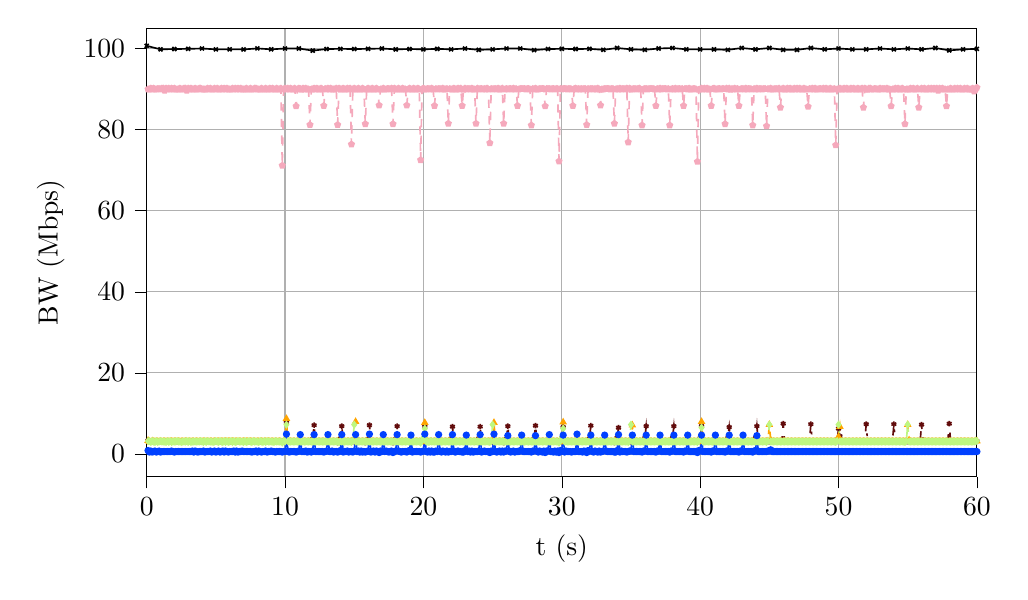
\begin{tikzpicture}

\definecolor{blue064255}{RGB}{0,64,255}
\definecolor{darkgrey176}{RGB}{176,176,176}
\definecolor{lightpink245169188}{RGB}{245,169,188}
\definecolor{maroon971111}{RGB}{97,11,11}
\definecolor{orange}{RGB}{255,165,0}
\definecolor{palegreen190247129}{RGB}{190,247,129}

\begin{axis}[
height=0.6\textwidth,
tick align=outside,
tick pos=left,
width=\textwidth,
x grid style={darkgrey176},
xlabel={t (s)},
xmajorgrids,
xmin=0, xmax=60,
xtick style={color=black},
y grid style={darkgrey176},
ylabel={BW (Mbps)},
ymajorgrids,
ymin=-5.54886786684783, ymax=105,
ytick style={color=black}
]
\addplot [semithick, maroon971111, dash pattern=on 1pt off 3pt on 3pt off 3pt, mark=asterisk, mark size=1, mark options={solid}]
table {%
0.1 3.32258152173913
0.2 3.07182065217391
0.3 3.07182065217391
0.4 3.07182065217391
0.5 3.07182065217391
0.6 3.07182065217391
0.7 3.07182065217391
0.8 3.07182065217391
0.9 3.07182065217391
1 3.07182065217391
1.1 3.07182065217391
1.2 3.07182065217391
1.3 3.07182065217391
1.4 3.07182065217391
1.5 3.07182065217391
1.6 3.07182065217391
1.7 3.07182065217391
1.8 3.07182065217391
1.9 3.07182065217391
2 3.07182065217391
2.1 3.07182065217391
2.2 3.07182065217391
2.3 3.07182065217391
2.4 3.07182065217391
2.5 3.07182065217391
2.6 3.07182065217391
2.7 3.07182065217391
2.8 3.07182065217391
2.9 3.07182065217391
3 3.07182065217391
3.1 3.07182065217391
3.2 3.07182065217391
3.3 3.07182065217391
3.4 3.07182065217391
3.5 3.07182065217391
3.6 3.07182065217391
3.7 3.07182065217391
3.8 3.07182065217391
3.9 3.07182065217391
4 3.07182065217391
4.1 3.07182065217391
4.2 3.07182065217391
4.3 3.07182065217391
4.4 3.07182065217391
4.5 3.07182065217391
4.6 3.07182065217391
4.7 3.07182065217391
4.8 3.07182065217391
4.9 3.07182065217391
5 3.07182065217391
5.1 3.07182065217391
5.2 3.07182065217391
5.3 3.07182065217391
5.4 3.07182065217391
5.5 3.07182065217391
5.6 3.07182065217391
5.7 3.07182065217391
5.8 3.07182065217391
5.9 3.07182065217391
6 3.07182065217391
6.1 3.07182065217391
6.2 3.07182065217391
6.3 3.07182065217391
6.4 3.07182065217391
6.5 3.07182065217391
6.6 3.07182065217391
6.7 3.07182065217391
6.8 3.07182065217391
6.9 3.07182065217391
7 3.07182065217391
7.1 3.07182065217391
7.2 3.07182065217391
7.3 3.07182065217391
7.4 3.07182065217391
7.5 3.07182065217391
7.6 3.07182065217391
7.7 3.07182065217391
7.8 3.07182065217391
7.9 3.07182065217391
8 3.07182065217391
8.1 3.07182065217391
8.2 3.07182065217391
8.3 3.07182065217391
8.4 3.07182065217391
8.5 3.07182065217391
8.6 3.07182065217391
8.7 3.07182065217391
8.8 3.07182065217391
8.9 3.07182065217391
9 3.07182065217391
9.1 3.07182065217391
9.2 3.07182065217391
9.3 3.07182065217391
9.4 3.07182065217391
9.5 3.07182065217391
9.6 3.07182065217391
9.7 3.07182065217391
9.8 2.9464402173913
9.9 3.19720108695652
10 3.07182065217391
10.1 7.86762228260869
10.2 3.07182065217391
10.3 3.07182065217391
10.4 3.07182065217391
10.5 3.07182065217391
10.6 3.07182065217391
10.7 3.07182065217391
10.8 3.07182065217391
10.9 3.07182065217391
11 3.07182065217391
11.1 3.07182065217391
11.2 3.07182065217391
11.3 3.07182065217391
11.4 3.07182065217391
11.5 3.07182065217391
11.6 3.07182065217391
11.7 3.07182065217391
11.8 2.9464402173913
11.9 3.32049184782609
12 3.6861847826087
12.1 7.12578804347826
12.2 3.07182065217391
12.3 3.07182065217391
12.4 3.07182065217391
12.5 3.07182065217391
12.6 3.07182065217391
12.7 3.07182065217391
12.8 3.07182065217391
12.9 3.07182065217391
13 3.07182065217391
13.1 3.07182065217391
13.2 3.07182065217391
13.3 3.07182065217391
13.4 3.07182065217391
13.5 3.07182065217391
13.6 3.07182065217391
13.7 3.07182065217391
13.8 2.8210597826087
13.9 3.32049184782609
14 3.80947554347826
14.1 6.88547554347826
14.2 3.07182065217391
14.3 3.07182065217391
14.4 3.07182065217391
14.5 3.07182065217391
14.6 3.07182065217391
14.7 3.07182065217391
14.8 2.9464402173913
14.9 3.19720108695652
15 3.07182065217391
15.1 3.07182065217391
15.2 3.07182065217391
15.3 3.07182065217391
15.4 3.07182065217391
15.5 3.07182065217391
15.6 3.07182065217391
15.7 3.07182065217391
15.8 2.8210597826087
15.9 3.32049184782609
16 3.6861847826087
16.1 7.12578804347826
16.2 3.07182065217391
16.3 3.07182065217391
16.4 3.07182065217391
16.5 3.07182065217391
16.6 3.07182065217391
16.7 3.07182065217391
16.8 3.07182065217391
16.9 3.07182065217391
17 3.07182065217391
17.1 3.07182065217391
17.2 3.07182065217391
17.3 3.07182065217391
17.4 3.07182065217391
17.5 3.07182065217391
17.6 3.07182065217391
17.7 3.07182065217391
17.8 2.8210597826087
17.9 3.32049184782609
18 3.6861847826087
18.1 6.88547554347826
18.2 3.07182065217391
18.3 3.07182065217391
18.4 3.07182065217391
18.5 3.07182065217391
18.6 3.07182065217391
18.7 3.07182065217391
18.8 3.07182065217391
18.9 3.07182065217391
19 3.07182065217391
19.1 3.07182065217391
19.2 3.07182065217391
19.3 3.07182065217391
19.4 3.07182065217391
19.5 3.07182065217391
19.6 3.07182065217391
19.7 3.07182065217391
19.8 2.9464402173913
19.9 3.32049184782609
20 3.6861847826087
20.1 6.88547554347826
20.2 3.07182065217391
20.3 3.07182065217391
20.4 3.07182065217391
20.5 3.07182065217391
20.6 3.07182065217391
20.7 3.07182065217391
20.8 3.07182065217391
20.9 3.07182065217391
21 3.07182065217391
21.1 3.07182065217391
21.2 3.07182065217391
21.3 3.07182065217391
21.4 3.07182065217391
21.5 3.07182065217391
21.6 3.07182065217391
21.7 3.07182065217391
21.8 2.9464402173913
21.9 3.19511141304348
22 3.80947554347826
22.1 6.76009510869565
22.2 3.07182065217391
22.3 3.07182065217391
22.4 3.07182065217391
22.5 3.07182065217391
22.6 3.07182065217391
22.7 3.07182065217391
22.8 3.07182065217391
22.9 3.07182065217391
23 3.07182065217391
23.1 3.07182065217391
23.2 3.07182065217391
23.3 3.07182065217391
23.4 3.07182065217391
23.5 3.07182065217391
23.6 3.07182065217391
23.7 3.07182065217391
23.8 2.9464402173913
23.9 3.19511141304348
24 3.80947554347826
24.1 6.76009510869565
24.2 3.07182065217391
24.3 3.07182065217391
24.4 3.07182065217391
24.5 3.07182065217391
24.6 3.07182065217391
24.7 3.07182065217391
24.8 3.07182065217391
24.9 3.07182065217391
25 3.07182065217391
25.1 3.07182065217391
25.2 3.07182065217391
25.3 3.07182065217391
25.4 3.07182065217391
25.5 3.07182065217391
25.6 3.07182065217391
25.7 3.07182065217391
25.8 2.8210597826087
25.9 3.32049184782609
26 3.6861847826087
26.1 6.88547554347826
26.2 3.07182065217391
26.3 3.07182065217391
26.4 3.07182065217391
26.5 3.07182065217391
26.6 3.07182065217391
26.7 3.07182065217391
26.8 3.07182065217391
26.9 3.07182065217391
27 3.07182065217391
27.1 3.07182065217391
27.2 3.07182065217391
27.3 3.07182065217391
27.4 3.07182065217391
27.5 3.07182065217391
27.6 3.07182065217391
27.7 3.07182065217391
27.8 3.07182065217391
27.9 3.19511141304348
28 3.80947554347826
28.1 7.00040760869565
28.2 3.07182065217391
28.3 3.07182065217391
28.4 3.07182065217391
28.5 3.07182065217391
28.6 3.07182065217391
28.7 3.07182065217391
28.8 3.07182065217391
28.9 3.07182065217391
29 3.07182065217391
29.1 3.07182065217391
29.2 3.07182065217391
29.3 3.07182065217391
29.4 3.07182065217391
29.5 3.07182065217391
29.6 3.07182065217391
29.7 3.07182065217391
29.8 2.9464402173913
29.9 3.32049184782609
30 3.9317214673913
30.1 6.63471467391304
30.2 3.07182065217391
30.3 3.07182065217391
30.4 3.07182065217391
30.5 3.07182065217391
30.6 3.07182065217391
30.7 3.07182065217391
30.8 3.07182065217391
30.9 3.07182065217391
31 3.07182065217391
31.1 3.07182065217391
31.2 3.07182065217391
31.3 3.07182065217391
31.4 3.07182065217391
31.5 3.07182065217391
31.6 3.07182065217391
31.7 3.07182065217391
31.8 2.9464402173913
31.9 3.19511141304348
32 3.80947554347826
32.1 7.00040760869565
32.2 3.07182065217391
32.3 3.07182065217391
32.4 3.07182065217391
32.5 3.07182065217391
32.6 3.07182065217391
32.7 3.07182065217391
32.8 3.07182065217391
32.9 3.07182065217391
33 3.07182065217391
33.1 3.07182065217391
33.2 3.07182065217391
33.3 3.07182065217391
33.4 3.07182065217391
33.5 3.07182065217391
33.6 3.07182065217391
33.7 3.07182065217391
33.8 2.8210597826087
33.9 3.32049184782609
34 4.05501222826087
34.1 6.50933423913043
34.2 3.07182065217391
34.3 3.07182065217391
34.4 3.07182065217391
34.5 3.07182065217391
34.6 3.07182065217391
34.7 3.07182065217391
34.8 3.07182065217391
34.9 3.07182065217391
35 3.07182065217391
35.1 3.07182065217391
35.2 3.07182065217391
35.3 3.07182065217391
35.4 3.07182065217391
35.5 3.07182065217391
35.6 3.07182065217391
35.7 3.07182065217391
35.8 3.07182065217391
35.9 3.19511141304348
36 3.9317214673913
36.1 6.88547554347826
36.2 3.07182065217391
36.3 3.07182065217391
36.4 3.07182065217391
36.5 3.07182065217391
36.6 3.07182065217391
36.7 3.07182065217391
36.8 3.07182065217391
36.9 3.07182065217391
37 3.07182065217391
37.1 3.07182065217391
37.2 3.07182065217391
37.3 3.07182065217391
37.4 3.07182065217391
37.5 3.07182065217391
37.6 3.07182065217391
37.7 3.07182065217391
37.8 3.07182065217391
37.9 3.19511141304348
38 3.9317214673913
38.1 6.88547554347826
38.2 3.07182065217391
38.3 3.07182065217391
38.4 3.07182065217391
38.5 3.07182065217391
38.6 3.07182065217391
38.7 3.07182065217391
38.8 3.07182065217391
38.9 3.07182065217391
39 3.07182065217391
39.1 3.07182065217391
39.2 3.07182065217391
39.3 3.07182065217391
39.4 3.07182065217391
39.5 3.07182065217391
39.6 3.07182065217391
39.7 3.07182065217391
39.8 2.9464402173913
39.9 3.32049184782609
40 3.9317214673913
40.1 6.88547554347826
40.2 3.07182065217391
40.3 3.07182065217391
40.4 3.07182065217391
40.5 3.07182065217391
40.6 3.07182065217391
40.7 3.07182065217391
40.8 3.07182065217391
40.9 3.07182065217391
41 3.07182065217391
41.1 3.07182065217391
41.2 3.07182065217391
41.3 3.07182065217391
41.4 3.07182065217391
41.5 3.07182065217391
41.6 3.07182065217391
41.7 3.07182065217391
41.8 2.9464402173913
41.9 3.19511141304348
42 3.9317214673913
42.1 6.63471467391304
42.2 3.07182065217391
42.3 3.07182065217391
42.4 3.07182065217391
42.5 3.07182065217391
42.6 3.07182065217391
42.7 3.07182065217391
42.8 3.07182065217391
42.9 3.07182065217391
43 3.07182065217391
43.1 3.07182065217391
43.2 3.07182065217391
43.3 3.07182065217391
43.4 3.07182065217391
43.5 3.07182065217391
43.6 3.07182065217391
43.7 3.07182065217391
43.8 3.07182065217391
43.9 3.19511141304348
44 3.9317214673913
44.1 6.88547554347826
44.2 3.07182065217391
44.3 3.07182065217391
44.4 3.07182065217391
44.5 3.07182065217391
44.6 3.07182065217391
44.7 3.07182065217391
44.8 3.07182065217391
44.9 3.07182065217391
45 3.07182065217391
45.1 3.07182065217391
45.2 3.07182065217391
45.3 2.9464402173913
45.4 3.19720108695652
45.5 3.07182065217391
45.6 3.07182065217391
45.7 3.07182065217391
45.8 2.9464402173913
45.9 3.19511141304348
46 7.49148097826087
46.1 3.07182065217391
46.2 3.07182065217391
46.3 3.07182065217391
46.4 3.07182065217391
46.5 3.07182065217391
46.6 3.07182065217391
46.7 3.07182065217391
46.8 3.07182065217391
46.9 3.07182065217391
47 3.07182065217391
47.1 3.07182065217391
47.2 3.07182065217391
47.3 3.07182065217391
47.4 3.07182065217391
47.5 3.07182065217391
47.6 3.07182065217391
47.7 3.07182065217391
47.8 2.9464402173913
47.9 3.19511141304348
48 7.37654891304348
48.1 3.19511141304348
48.2 3.07182065217391
48.3 3.07182065217391
48.4 3.07182065217391
48.5 3.07182065217391
48.6 3.07182065217391
48.7 3.07182065217391
48.8 3.07182065217391
48.9 3.07182065217391
49 3.07182065217391
49.1 3.07182065217391
49.2 3.07182065217391
49.3 3.07182065217391
49.4 3.07182065217391
49.5 3.07182065217391
49.6 3.07182065217391
49.7 3.07182065217391
49.8 3.07182065217391
49.9 3.19511141304348
50 6.26902173913043
50.1 4.41966032608696
50.2 3.07182065217391
50.3 3.07182065217391
50.4 3.07182065217391
50.5 3.07182065217391
50.6 3.07182065217391
50.7 3.07182065217391
50.8 3.07182065217391
50.9 3.07182065217391
51 3.07182065217391
51.1 3.07182065217391
51.2 3.07182065217391
51.3 3.07182065217391
51.4 3.07182065217391
51.5 3.07182065217391
51.6 3.07182065217391
51.7 3.07182065217391
51.8 2.9464402173913
51.9 3.19511141304348
52 7.37654891304348
52.1 3.19511141304348
52.2 3.07182065217391
52.3 3.07182065217391
52.4 3.07182065217391
52.5 3.07182065217391
52.6 3.07182065217391
52.7 3.07182065217391
52.8 3.07182065217391
52.9 3.07182065217391
53 3.07182065217391
53.1 3.07182065217391
53.2 3.07182065217391
53.3 3.07182065217391
53.4 3.07182065217391
53.5 3.07182065217391
53.6 3.07182065217391
53.7 3.07182065217391
53.8 2.9464402173913
53.9 3.19511141304348
54 7.37654891304348
54.1 3.19511141304348
54.2 3.07182065217391
54.3 3.07182065217391
54.4 3.07182065217391
54.5 3.07182065217391
54.6 3.07182065217391
54.7 3.07182065217391
54.8 3.07182065217391
54.9 3.07182065217391
55 3.07182065217391
55.1 3.07182065217391
55.2 3.07182065217391
55.3 3.07182065217391
55.4 3.07182065217391
55.5 3.07182065217391
55.6 3.07182065217391
55.7 3.07182065217391
55.8 2.9464402173913
55.9 3.19511141304348
56 7.25116847826087
56.1 3.31735733695652
56.2 3.07182065217391
56.3 3.07182065217391
56.4 3.07182065217391
56.5 3.07182065217391
56.6 3.07182065217391
56.7 3.07182065217391
56.8 3.07182065217391
56.9 3.07182065217391
57 3.07182065217391
57.1 3.07182065217391
57.2 3.07182065217391
57.3 3.07182065217391
57.4 3.07182065217391
57.5 3.07182065217391
57.6 3.07182065217391
57.7 3.07182065217391
57.8 2.9464402173913
57.9 3.19511141304348
58 7.49148097826087
58.1 3.07182065217391
58.2 3.07182065217391
58.3 3.07182065217391
58.4 3.07182065217391
58.5 3.07182065217391
58.6 3.07182065217391
58.7 3.07182065217391
58.8 3.07182065217391
58.9 3.07182065217391
59 3.07182065217391
59.1 3.07182065217391
59.2 3.07182065217391
59.3 3.07182065217391
59.4 3.07182065217391
59.5 3.07182065217391
59.6 3.07182065217391
59.7 3.07182065217391
59.8 3.07182065217391
59.9 3.19511141304348
60 3.20138043478261
};
\addplot [semithick, lightpink245169188, dashed, mark=pentagon*, mark size=1, mark options={solid}]
table {%
0.1 89.9604619565217
0.2 89.9604619565217
0.3 90.1694293478261
0.4 89.9604619565217
0.5 90.1694293478261
0.6 89.9604619565217
0.7 89.9604619565217
0.8 90.0649456521739
0.9 90.0649456521739
1 89.9604619565217
1.1 90.1694293478261
1.2 90.1694293478261
1.3 89.6470108695652
1.4 90.1694293478261
1.5 89.9604619565217
1.6 90.1694293478261
1.7 89.9604619565217
1.8 90.1694293478261
1.9 89.9604619565217
2 90.1694293478261
2.1 89.9604619565217
2.2 89.9604619565217
2.3 89.9604619565217
2.4 90.1694293478261
2.5 89.9604619565217
2.6 89.9604619565217
2.7 90.1694293478261
2.8 90.1694293478261
2.9 89.6470108695652
3 90.1694293478261
3.1 89.9604619565217
3.2 90.1694293478261
3.3 89.9604619565217
3.4 89.9604619565217
3.5 90.1694293478261
3.6 89.9604619565217
3.7 89.9604619565217
3.8 90.1694293478261
3.9 90.1694293478261
4 89.9604619565217
4.1 89.9604619565217
4.2 89.9604619565217
4.3 89.9604619565217
4.4 90.1694293478261
4.5 89.9604619565217
4.6 90.1694293478261
4.7 89.9604619565217
4.8 89.9604619565217
4.9 90.1694293478261
5 89.9604619565217
5.1 90.1694293478261
5.2 89.9604619565217
5.3 89.9604619565217
5.4 90.1694293478261
5.5 89.9604619565217
5.6 90.1694293478261
5.7 89.9604619565217
5.8 90.1694293478261
5.9 89.9604619565217
6 89.9604619565217
6.1 89.9604619565217
6.2 90.1694293478261
6.3 89.9604619565217
6.4 90.1694293478261
6.5 89.9604619565217
6.6 90.1694293478261
6.7 89.9604619565217
6.8 90.1694293478261
6.9 89.9604619565217
7 89.9604619565217
7.1 89.9604619565217
7.2 90.1694293478261
7.3 89.9604619565217
7.4 89.9604619565217
7.5 90.1694293478261
7.6 89.9604619565217
7.7 89.9604619565217
7.8 90.1694293478261
7.9 90.1694293478261
8 89.9604619565217
8.1 89.9604619565217
8.2 89.9604619565217
8.3 90.1694293478261
8.4 89.9604619565217
8.5 89.9604619565217
8.6 90.1694293478261
8.7 89.9604619565217
8.8 89.9604619565217
8.9 90.1694293478261
9 89.9604619565217
9.1 90.1694293478261
9.2 89.9604619565217
9.3 89.9604619565217
9.4 90.1694293478261
9.5 89.9604619565217
9.6 89.9604619565217
9.7 90.1694293478261
9.8 71.1533967391304
9.9 89.9604619565217
10 90.1694293478261
10.1 89.9604619565217
10.2 90.1694293478261
10.3 89.9604619565217
10.4 90.1694293478261
10.5 89.9604619565217
10.6 89.9604619565217
10.7 90.1694293478261
10.8 85.7811141304348
10.9 89.9604619565217
11 90.1694293478261
11.1 90.0649456521739
11.2 89.8559782608696
11.3 90.1694293478261
11.4 89.9604619565217
11.5 90.1694293478261
11.6 89.9604619565217
11.7 89.9604619565217
11.8 81.1838315217391
11.9 89.9604619565217
12 89.9604619565217
12.1 90.1694293478261
12.2 89.9604619565217
12.3 90.1694293478261
12.4 89.9604619565217
12.5 89.9604619565217
12.6 90.1694293478261
12.7 89.9604619565217
12.8 85.885597826087
12.9 90.0649456521739
13 89.9604619565217
13.1 90.1694293478261
13.2 89.9604619565217
13.3 90.1694293478261
13.4 89.9604619565217
13.5 89.9604619565217
13.6 89.9604619565217
13.7 90.1694293478261
13.8 81.1838315217391
13.9 90.1694293478261
14 89.9604619565217
14.1 89.9604619565217
14.2 90.1694293478261
14.3 89.9604619565217
14.4 89.9604619565217
14.5 90.1694293478261
14.6 89.9604619565217
14.7 90.1694293478261
14.8 76.3775815217391
14.9 89.9604619565217
15 90.1694293478261
15.1 89.9604619565217
15.2 89.9604619565217
15.3 90.1694293478261
15.4 89.9604619565217
15.5 89.9604619565217
15.6 90.1694293478261
15.7 89.9604619565217
15.8 81.3927989130435
15.9 89.9604619565217
16 90.1694293478261
16.1 89.9604619565217
16.2 89.9604619565217
16.3 90.1694293478261
16.4 89.9604619565217
16.5 89.9604619565217
16.6 90.1694293478261
16.7 89.9604619565217
16.8 85.9900815217391
16.9 89.9604619565217
17 89.9604619565217
17.1 90.1694293478261
17.2 89.9604619565217
17.3 89.9604619565217
17.4 90.0649456521739
17.5 90.0649456521739
17.6 89.9604619565217
17.7 90.1694293478261
17.8 81.3927989130435
17.9 90.1694293478261
18 89.9604619565217
18.1 89.9604619565217
18.2 90.1694293478261
18.3 89.9604619565217
18.4 89.9604619565217
18.5 90.1694293478261
18.6 89.9604619565217
18.7 89.9604619565217
18.8 85.9900815217391
18.9 89.9604619565217
19 90.1694293478261
19.1 89.9604619565217
19.2 89.9604619565217
19.3 90.1694293478261
19.4 89.9604619565217
19.5 89.9604619565217
19.6 90.1694293478261
19.7 89.9604619565217
19.8 72.5116847826087
19.9 89.9604619565217
20 90.1694293478261
20.1 89.9604619565217
20.2 89.9604619565217
20.3 90.0649456521739
20.4 90.0649456521739
20.5 89.9604619565217
20.6 90.1694293478261
20.7 89.9604619565217
20.8 85.885597826087
20.9 90.0649456521739
21 89.9604619565217
21.1 90.0649456521739
21.2 90.0649456521739
21.3 89.9604619565217
21.4 90.1694293478261
21.5 89.9604619565217
21.6 89.9604619565217
21.7 90.0649456521739
21.8 81.4972826086956
21.9 90.0649456521739
22 89.9604619565217
22.1 89.9604619565217
22.2 90.1694293478261
22.3 89.9604619565217
22.4 89.9604619565217
22.5 90.1694293478261
22.6 89.9604619565217
22.7 90.1694293478261
22.8 85.885597826087
22.9 89.8559782608696
23 90.1694293478261
23.1 89.9604619565217
23.2 90.0649456521739
23.3 90.0649456521739
23.4 89.9604619565217
23.5 90.1694293478261
23.6 89.9604619565217
23.7 89.9604619565217
23.8 81.4972826086956
23.9 90.1694293478261
24 89.9604619565217
24.1 90.0649456521739
24.2 90.0649456521739
24.3 89.9604619565217
24.4 90.0649456521739
24.5 89.9604619565217
24.6 90.1694293478261
24.7 89.9604619565217
24.8 76.6910326086957
24.9 90.0649456521739
25 89.9604619565217
25.1 90.0649456521739
25.2 90.0649456521739
25.3 89.9604619565217
25.4 90.1694293478261
25.5 89.9604619565217
25.6 89.9604619565217
25.7 90.1694293478261
25.8 81.4972826086956
25.9 89.9604619565217
26 90.0649456521739
26.1 89.9604619565217
26.2 90.0649456521739
26.3 90.0649456521739
26.4 89.9604619565217
26.5 90.1694293478261
26.6 89.9604619565217
26.7 90.0649456521739
26.8 85.885597826087
26.9 89.9604619565217
27 90.0649456521739
27.1 90.0649456521739
27.2 90.0649456521739
27.3 90.0649456521739
27.4 89.9604619565217
27.5 90.0649456521739
27.6 90.0649456521739
27.7 89.9604619565217
27.8 81.0793478260869
27.9 90.0649456521739
28 89.9604619565217
28.1 90.1694293478261
28.2 89.9604619565217
28.3 89.9604619565217
28.4 90.0649456521739
28.5 90.0649456521739
28.6 90.0649456521739
28.7 90.0649456521739
28.8 85.7811141304348
28.9 90.0649456521739
29 90.0649456521739
29.1 90.0649456521739
29.2 89.9604619565217
29.3 90.0649456521739
29.4 90.0649456521739
29.5 89.9604619565217
29.6 90.0649456521739
29.7 90.0649456521739
29.8 72.1982336956522
29.9 90.0649456521739
30 89.9604619565217
30.1 90.0649456521739
30.2 90.0649456521739
30.3 90.0649456521739
30.4 89.9604619565217
30.5 90.0649456521739
30.6 90.0649456521739
30.7 89.9604619565217
30.8 85.885597826087
30.9 90.0649456521739
31 90.1694293478261
31.1 89.9604619565217
31.2 90.0649456521739
31.3 89.9604619565217
31.4 90.0649456521739
31.5 89.9604619565217
31.6 90.0649456521739
31.7 90.0649456521739
31.8 81.1838315217391
31.9 90.0649456521739
32 89.9604619565217
32.1 90.0649456521739
32.2 90.0649456521739
32.3 89.9604619565217
32.4 90.0649456521739
32.5 89.9604619565217
32.6 90.1694293478261
32.7 89.9604619565217
32.8 85.9900815217391
32.9 89.9604619565217
33 89.9604619565217
33.1 90.0649456521739
33.2 90.0649456521739
33.3 90.0649456521739
33.4 90.0649456521739
33.5 89.9604619565217
33.6 90.0649456521739
33.7 90.0649456521739
33.8 81.4972826086956
33.9 89.9604619565217
34 90.0649456521739
34.1 89.9604619565217
34.2 90.1694293478261
34.3 89.9604619565217
34.4 90.0649456521739
34.5 90.0649456521739
34.6 89.9604619565217
34.7 90.1694293478261
34.8 76.9
34.9 90.1694293478261
35 89.9604619565217
35.1 89.9604619565217
35.2 90.0649456521739
35.3 90.0649456521739
35.4 89.9604619565217
35.5 90.0649456521739
35.6 90.1694293478261
35.7 89.9604619565217
35.8 81.0793478260869
35.9 89.9604619565217
36 90.0649456521739
36.1 90.0649456521739
36.2 89.9604619565217
36.3 90.0649456521739
36.4 90.0649456521739
36.5 90.0649456521739
36.6 90.0649456521739
36.7 89.9604619565217
36.8 85.885597826087
36.9 90.0649456521739
37 89.9604619565217
37.1 90.1694293478261
37.2 89.9604619565217
37.3 90.0649456521739
37.4 90.0649456521739
37.5 90.0649456521739
37.6 89.9604619565217
37.7 90.0649456521739
37.8 81.0793478260869
37.9 89.9604619565217
38 90.0649456521739
38.1 89.9604619565217
38.2 90.1694293478261
38.3 89.9604619565217
38.4 90.0649456521739
38.5 90.0649456521739
38.6 89.9604619565217
38.7 90.0649456521739
38.8 85.885597826087
38.9 90.0649456521739
39 90.0649456521739
39.1 89.9604619565217
39.2 90.1694293478261
39.3 89.9604619565217
39.4 89.9604619565217
39.5 90.0649456521739
39.6 90.0649456521739
39.7 89.9604619565217
39.8 72.09375
39.9 89.8559782608696
40 89.9604619565217
40.1 90.1694293478261
40.2 89.9604619565217
40.3 90.1694293478261
40.4 89.9604619565217
40.5 90.1694293478261
40.6 89.9604619565217
40.7 89.9604619565217
40.8 85.885597826087
40.9 90.0649456521739
41 90.1694293478261
41.1 89.9604619565217
41.2 89.9604619565217
41.3 90.0649456521739
41.4 90.0649456521739
41.5 89.9604619565217
41.6 90.0649456521739
41.7 90.0649456521739
41.8 81.3927989130435
41.9 90.1694293478261
42 89.9604619565217
42.1 90.1694293478261
42.2 89.8559782608696
42.3 90.0649456521739
42.4 89.9604619565217
42.5 90.1694293478261
42.6 89.9604619565217
42.7 90.0649456521739
42.8 85.885597826087
42.9 89.9604619565217
43 90.0649456521739
43.1 90.0649456521739
43.2 89.9604619565217
43.3 90.1694293478261
43.4 89.9604619565217
43.5 90.0649456521739
43.6 90.0649456521739
43.7 89.9604619565217
43.8 81.0793478260869
43.9 90.0649456521739
44 89.9604619565217
44.1 90.1694293478261
44.2 89.9604619565217
44.3 90.0649456521739
44.4 90.0649456521739
44.5 89.9604619565217
44.6 90.0649456521739
44.7 90.0649456521739
44.8 80.8703804347826
44.9 90.0649456521739
45 89.9604619565217
45.1 90.1694293478261
45.2 89.9604619565217
45.3 89.9604619565217
45.4 90.0649456521739
45.5 90.0649456521739
45.6 89.9604619565217
45.7 90.1694293478261
45.8 85.4676630434783
45.9 89.9604619565217
46 90.1694293478261
46.1 89.9604619565217
46.2 89.9604619565217
46.3 90.1694293478261
46.4 89.9604619565217
46.5 90.1694293478261
46.6 89.9604619565217
46.7 89.9604619565217
46.8 90.1694293478261
46.9 89.9604619565217
47 90.1694293478261
47.1 89.9604619565217
47.2 90.1694293478261
47.3 89.9604619565217
47.4 89.9604619565217
47.5 90.1694293478261
47.6 89.9604619565217
47.7 89.9604619565217
47.8 85.6766304347826
47.9 90.0649456521739
48 89.9604619565217
48.1 90.1694293478261
48.2 89.9604619565217
48.3 90.1694293478261
48.4 89.9604619565217
48.5 89.9604619565217
48.6 90.0649456521739
48.7 90.0649456521739
48.8 89.9604619565217
48.9 90.1694293478261
49 89.9604619565217
49.1 90.1694293478261
49.2 89.9604619565217
49.3 89.9604619565217
49.4 90.1694293478261
49.5 89.9604619565217
49.6 89.9604619565217
49.7 90.0649456521739
49.8 76.1686141304348
49.9 89.9604619565217
50 89.9604619565217
50.1 90.1694293478261
50.2 89.9604619565217
50.3 89.9604619565217
50.4 90.1694293478261
50.5 89.9604619565217
50.6 90.1694293478261
50.7 89.9604619565217
50.8 89.9604619565217
50.9 90.1694293478261
51 89.9604619565217
51.1 90.1694293478261
51.2 89.9604619565217
51.3 89.9604619565217
51.4 90.1694293478261
51.5 89.9604619565217
51.6 89.9604619565217
51.7 90.1694293478261
51.8 85.4676630434783
51.9 90.1694293478261
52 89.9604619565217
52.1 89.8559782608696
52.2 90.1694293478261
52.3 90.1694293478261
52.4 89.9604619565217
52.5 89.9604619565217
52.6 90.0649456521739
52.7 90.0649456521739
52.8 89.9604619565217
52.9 89.9604619565217
53 90.1694293478261
53.1 89.9604619565217
53.2 90.0649456521739
53.3 90.0649456521739
53.4 89.9604619565217
53.5 90.1694293478261
53.6 89.9604619565217
53.7 89.9604619565217
53.8 85.7811141304348
53.9 89.9604619565217
54 89.9604619565217
54.1 90.1694293478261
54.2 89.9604619565217
54.3 90.1694293478261
54.4 89.9604619565217
54.5 89.9604619565217
54.6 90.1694293478261
54.7 89.9604619565217
54.8 81.3927989130435
54.9 89.9604619565217
55 89.9604619565217
55.1 89.9604619565217
55.2 90.1694293478261
55.3 89.9604619565217
55.4 90.1694293478261
55.5 89.9604619565217
55.6 89.9604619565217
55.7 90.1694293478261
55.8 85.4676630434783
55.9 89.9604619565217
56 90.1694293478261
56.1 89.9604619565217
56.2 90.1694293478261
56.3 89.9604619565217
56.4 89.9604619565217
56.5 90.1694293478261
56.6 89.9604619565217
56.7 90.1694293478261
56.8 89.9604619565217
56.9 90.1694293478261
57 89.9604619565217
57.1 90.1694293478261
57.2 89.6470108695652
57.3 90.1694293478261
57.4 89.9604619565217
57.5 90.1694293478261
57.6 89.9604619565217
57.7 89.9604619565217
57.8 85.7811141304348
57.9 89.9604619565217
58 89.9604619565217
58.1 90.1694293478261
58.2 89.9604619565217
58.3 89.9604619565217
58.4 90.1694293478261
58.5 89.9604619565217
58.6 90.1694293478261
58.7 89.9604619565217
58.8 90.1694293478261
58.9 89.9604619565217
59 89.9604619565217
59.1 90.1694293478261
59.2 89.9604619565217
59.3 90.1694293478261
59.4 89.9604619565217
59.5 89.9604619565217
59.6 89.9604619565217
59.7 90.1694293478261
59.8 89.4380434782609
59.9 89.8559782608696
60 90.3783967391304
};
\addplot [semithick, orange, dashed, mark=triangle*, mark size=1, mark options={solid}]
table {%
0.1 3.32258152173913
0.2 3.07182065217391
0.3 2.9464402173913
0.4 3.19720108695652
0.5 3.07182065217391
0.6 3.07182065217391
0.7 3.07182065217391
0.8 3.07182065217391
0.9 3.07182065217391
1 3.07182065217391
1.1 3.07182065217391
1.2 3.07182065217391
1.3 3.07182065217391
1.4 3.07182065217391
1.5 3.07182065217391
1.6 3.07182065217391
1.7 3.07182065217391
1.8 3.07182065217391
1.9 3.07182065217391
2 3.07182065217391
2.1 3.07182065217391
2.2 3.07182065217391
2.3 3.07182065217391
2.4 3.07182065217391
2.5 3.07182065217391
2.6 3.07182065217391
2.7 3.07182065217391
2.8 3.07182065217391
2.9 3.07182065217391
3 3.07182065217391
3.1 3.07182065217391
3.2 3.07182065217391
3.3 3.07182065217391
3.4 3.07182065217391
3.5 3.07182065217391
3.6 3.07182065217391
3.7 3.07182065217391
3.8 3.07182065217391
3.9 3.07182065217391
4 3.07182065217391
4.1 3.07182065217391
4.2 3.07182065217391
4.3 3.07182065217391
4.4 3.07182065217391
4.5 3.07182065217391
4.6 3.07182065217391
4.7 3.07182065217391
4.8 3.07182065217391
4.9 3.07182065217391
5 3.07182065217391
5.1 3.07182065217391
5.2 3.07182065217391
5.3 3.07182065217391
5.4 3.07182065217391
5.5 3.07182065217391
5.6 3.07182065217391
5.7 3.07182065217391
5.8 3.07182065217391
5.9 3.07182065217391
6 3.07182065217391
6.1 3.07182065217391
6.2 3.07182065217391
6.3 3.07182065217391
6.4 3.07182065217391
6.5 3.07182065217391
6.6 3.07182065217391
6.7 3.07182065217391
6.8 3.07182065217391
6.9 3.07182065217391
7 3.07182065217391
7.1 3.07182065217391
7.2 3.07182065217391
7.3 3.07182065217391
7.4 3.07182065217391
7.5 3.07182065217391
7.6 3.07182065217391
7.7 3.07182065217391
7.8 3.07182065217391
7.9 3.07182065217391
8 3.07182065217391
8.1 3.07182065217391
8.2 3.07182065217391
8.3 3.07182065217391
8.4 3.07182065217391
8.5 3.07182065217391
8.6 3.07182065217391
8.7 3.07182065217391
8.8 3.07182065217391
8.9 3.07182065217391
9 3.07182065217391
9.1 3.07182065217391
9.2 3.07182065217391
9.3 3.07182065217391
9.4 3.07182065217391
9.5 3.07182065217391
9.6 3.07182065217391
9.7 3.07182065217391
9.8 2.9464402173913
9.9 3.19720108695652
10 3.07182065217391
10.1 8.72438858695652
10.2 3.07182065217391
10.3 3.07182065217391
10.4 3.07182065217391
10.5 3.07182065217391
10.6 3.07182065217391
10.7 3.07182065217391
10.8 3.07182065217391
10.9 3.07182065217391
11 3.07182065217391
11.1 3.07182065217391
11.2 3.07182065217391
11.3 3.07182065217391
11.4 3.07182065217391
11.5 3.07182065217391
11.6 3.07182065217391
11.7 3.07182065217391
11.8 3.07182065217391
11.9 3.07182065217391
12 3.07182065217391
12.1 3.07182065217391
12.2 3.07182065217391
12.3 3.07182065217391
12.4 3.07182065217391
12.5 3.07182065217391
12.6 3.07182065217391
12.7 3.07182065217391
12.8 3.07182065217391
12.9 3.07182065217391
13 3.07182065217391
13.1 3.07182065217391
13.2 3.07182065217391
13.3 3.07182065217391
13.4 3.07182065217391
13.5 3.07182065217391
13.6 3.07182065217391
13.7 3.07182065217391
13.8 3.07182065217391
13.9 3.07182065217391
14 3.07182065217391
14.1 3.07182065217391
14.2 3.07182065217391
14.3 3.07182065217391
14.4 3.07182065217391
14.5 3.07182065217391
14.6 3.07182065217391
14.7 3.07182065217391
14.8 3.07182065217391
14.9 3.19511141304348
15 3.19511141304348
15.1 7.98255434782609
15.2 3.07182065217391
15.3 3.07182065217391
15.4 3.07182065217391
15.5 3.07182065217391
15.6 3.07182065217391
15.7 3.07182065217391
15.8 3.07182065217391
15.9 3.07182065217391
16 3.07182065217391
16.1 3.07182065217391
16.2 3.07182065217391
16.3 3.07182065217391
16.4 3.07182065217391
16.5 3.07182065217391
16.6 3.07182065217391
16.7 3.07182065217391
16.8 3.07182065217391
16.9 3.07182065217391
17 3.07182065217391
17.1 3.07182065217391
17.2 3.07182065217391
17.3 3.07182065217391
17.4 3.07182065217391
17.5 3.07182065217391
17.6 3.07182065217391
17.7 3.07182065217391
17.8 3.07182065217391
17.9 3.07182065217391
18 3.07182065217391
18.1 3.07182065217391
18.2 3.07182065217391
18.3 3.07182065217391
18.4 3.07182065217391
18.5 3.07182065217391
18.6 3.07182065217391
18.7 3.07182065217391
18.8 3.07182065217391
18.9 3.07182065217391
19 3.07182065217391
19.1 3.07182065217391
19.2 3.07182065217391
19.3 3.07182065217391
19.4 3.07182065217391
19.5 3.07182065217391
19.6 3.07182065217391
19.7 3.07182065217391
19.8 2.9464402173913
19.9 3.19720108695652
20 3.19511141304348
20.1 7.74224184782609
20.2 3.07182065217391
20.3 3.07182065217391
20.4 3.07182065217391
20.5 3.07182065217391
20.6 3.07182065217391
20.7 3.07182065217391
20.8 3.07182065217391
20.9 3.07182065217391
21 3.07182065217391
21.1 3.07182065217391
21.2 3.07182065217391
21.3 3.07182065217391
21.4 3.07182065217391
21.5 3.07182065217391
21.6 3.07182065217391
21.7 3.07182065217391
21.8 3.07182065217391
21.9 3.07182065217391
22 3.07182065217391
22.1 3.07182065217391
22.2 3.07182065217391
22.3 3.07182065217391
22.4 3.07182065217391
22.5 3.07182065217391
22.6 3.07182065217391
22.7 3.07182065217391
22.8 3.07182065217391
22.9 3.07182065217391
23 3.07182065217391
23.1 3.07182065217391
23.2 3.07182065217391
23.3 3.07182065217391
23.4 3.07182065217391
23.5 3.07182065217391
23.6 3.07182065217391
23.7 3.07182065217391
23.8 3.07182065217391
23.9 3.07182065217391
24 3.07182065217391
24.1 3.07182065217391
24.2 3.07182065217391
24.3 3.07182065217391
24.4 3.07182065217391
24.5 3.07182065217391
24.6 3.07182065217391
24.7 3.07182065217391
24.8 3.07182065217391
24.9 3.19511141304348
25 3.31735733695652
25.1 7.74224184782609
25.2 3.07182065217391
25.3 3.07182065217391
25.4 3.07182065217391
25.5 3.07182065217391
25.6 3.07182065217391
25.7 3.07182065217391
25.8 3.07182065217391
25.9 3.07182065217391
26 3.07182065217391
26.1 3.07182065217391
26.2 3.07182065217391
26.3 3.07182065217391
26.4 3.07182065217391
26.5 3.07182065217391
26.6 3.07182065217391
26.7 3.07182065217391
26.8 3.07182065217391
26.9 3.07182065217391
27 3.07182065217391
27.1 3.07182065217391
27.2 3.07182065217391
27.3 3.07182065217391
27.4 3.07182065217391
27.5 3.07182065217391
27.6 3.07182065217391
27.7 3.07182065217391
27.8 3.07182065217391
27.9 3.07182065217391
28 3.07182065217391
28.1 3.07182065217391
28.2 3.07182065217391
28.3 3.07182065217391
28.4 3.07182065217391
28.5 3.07182065217391
28.6 3.07182065217391
28.7 3.07182065217391
28.8 3.07182065217391
28.9 3.07182065217391
29 3.07182065217391
29.1 3.07182065217391
29.2 3.07182065217391
29.3 3.07182065217391
29.4 3.07182065217391
29.5 3.07182065217391
29.6 3.07182065217391
29.7 3.07182065217391
29.8 2.9464402173913
29.9 3.19720108695652
30 3.19511141304348
30.1 7.86762228260869
30.2 3.07182065217391
30.3 3.07182065217391
30.4 3.07182065217391
30.5 3.07182065217391
30.6 3.07182065217391
30.7 3.07182065217391
30.8 3.07182065217391
30.9 3.07182065217391
31 3.07182065217391
31.1 3.07182065217391
31.2 3.07182065217391
31.3 3.07182065217391
31.4 3.07182065217391
31.5 3.07182065217391
31.6 3.07182065217391
31.7 3.07182065217391
31.8 3.07182065217391
31.9 3.07182065217391
32 3.07182065217391
32.1 3.07182065217391
32.2 3.07182065217391
32.3 3.07182065217391
32.4 3.07182065217391
32.5 3.07182065217391
32.6 3.07182065217391
32.7 3.07182065217391
32.8 3.07182065217391
32.9 3.07182065217391
33 3.07182065217391
33.1 3.07182065217391
33.2 3.07182065217391
33.3 3.07182065217391
33.4 3.07182065217391
33.5 3.07182065217391
33.6 3.07182065217391
33.7 3.07182065217391
33.8 3.07182065217391
33.9 3.07182065217391
34 3.07182065217391
34.1 3.07182065217391
34.2 3.07182065217391
34.3 3.07182065217391
34.4 3.07182065217391
34.5 3.07182065217391
34.6 3.07182065217391
34.7 3.07182065217391
34.8 3.07182065217391
34.9 3.19511141304348
35 3.56289402173913
35.1 7.12578804347826
35.2 3.07182065217391
35.3 3.07182065217391
35.4 3.07182065217391
35.5 3.07182065217391
35.6 3.07182065217391
35.7 3.07182065217391
35.8 3.07182065217391
35.9 3.07182065217391
36 3.07182065217391
36.1 3.07182065217391
36.2 3.07182065217391
36.3 3.07182065217391
36.4 3.07182065217391
36.5 3.07182065217391
36.6 3.07182065217391
36.7 3.07182065217391
36.8 3.07182065217391
36.9 3.07182065217391
37 3.07182065217391
37.1 3.07182065217391
37.2 3.07182065217391
37.3 3.07182065217391
37.4 3.07182065217391
37.5 3.07182065217391
37.6 3.07182065217391
37.7 3.07182065217391
37.8 3.07182065217391
37.9 3.07182065217391
38 3.07182065217391
38.1 3.07182065217391
38.2 3.07182065217391
38.3 3.07182065217391
38.4 3.07182065217391
38.5 3.07182065217391
38.6 3.07182065217391
38.7 3.07182065217391
38.8 3.07182065217391
38.9 3.07182065217391
39 3.07182065217391
39.1 3.07182065217391
39.2 3.07182065217391
39.3 3.07182065217391
39.4 3.07182065217391
39.5 3.07182065217391
39.6 3.07182065217391
39.7 3.07182065217391
39.8 2.9464402173913
39.9 3.19720108695652
40 3.19511141304348
40.1 7.98255434782609
40.2 3.07182065217391
40.3 3.07182065217391
40.4 3.07182065217391
40.5 3.07182065217391
40.6 3.07182065217391
40.7 3.07182065217391
40.8 3.07182065217391
40.9 3.07182065217391
41 3.07182065217391
41.1 3.07182065217391
41.2 3.07182065217391
41.3 3.07182065217391
41.4 3.07182065217391
41.5 3.07182065217391
41.6 3.07182065217391
41.7 3.07182065217391
41.8 3.07182065217391
41.9 3.07182065217391
42 3.07182065217391
42.1 3.07182065217391
42.2 3.07182065217391
42.3 3.07182065217391
42.4 3.07182065217391
42.5 3.07182065217391
42.6 3.07182065217391
42.7 3.07182065217391
42.8 3.07182065217391
42.9 3.07182065217391
43 3.07182065217391
43.1 3.07182065217391
43.2 3.07182065217391
43.3 3.07182065217391
43.4 3.07182065217391
43.5 3.07182065217391
43.6 3.07182065217391
43.7 3.07182065217391
43.8 3.07182065217391
43.9 3.07182065217391
44 3.07182065217391
44.1 3.07182065217391
44.2 3.07182065217391
44.3 3.07182065217391
44.4 3.07182065217391
44.5 3.07182065217391
44.6 3.07182065217391
44.7 3.07182065217391
44.8 3.07182065217391
44.9 3.19511141304348
45 7.25116847826087
45.1 3.44064809782609
45.2 3.07182065217391
45.3 3.07182065217391
45.4 3.07182065217391
45.5 3.07182065217391
45.6 3.07182065217391
45.7 3.07182065217391
45.8 3.07182065217391
45.9 3.07182065217391
46 3.07182065217391
46.1 3.07182065217391
46.2 3.07182065217391
46.3 3.07182065217391
46.4 3.07182065217391
46.5 3.07182065217391
46.6 3.07182065217391
46.7 3.07182065217391
46.8 3.07182065217391
46.9 3.07182065217391
47 3.07182065217391
47.1 3.07182065217391
47.2 3.07182065217391
47.3 3.07182065217391
47.4 3.07182065217391
47.5 3.07182065217391
47.6 3.07182065217391
47.7 3.07182065217391
47.8 3.07182065217391
47.9 3.07182065217391
48 3.07182065217391
48.1 3.07182065217391
48.2 3.07182065217391
48.3 3.07182065217391
48.4 3.07182065217391
48.5 3.07182065217391
48.6 3.07182065217391
48.7 3.07182065217391
48.8 3.07182065217391
48.9 3.07182065217391
49 3.07182065217391
49.1 3.07182065217391
49.2 3.07182065217391
49.3 3.07182065217391
49.4 3.07182065217391
49.5 3.07182065217391
49.6 3.07182065217391
49.7 3.07182065217391
49.8 3.07182065217391
49.9 3.19511141304348
50 4.30472826086956
50.1 6.76009510869565
50.2 3.07182065217391
50.3 3.07182065217391
50.4 3.07182065217391
50.5 3.07182065217391
50.6 3.07182065217391
50.7 3.07182065217391
50.8 3.07182065217391
50.9 3.07182065217391
51 3.07182065217391
51.1 3.07182065217391
51.2 3.07182065217391
51.3 3.07182065217391
51.4 3.07182065217391
51.5 3.07182065217391
51.6 3.07182065217391
51.7 3.07182065217391
51.8 3.07182065217391
51.9 3.07182065217391
52 3.07182065217391
52.1 3.07182065217391
52.2 3.07182065217391
52.3 3.07182065217391
52.4 3.07182065217391
52.5 3.07182065217391
52.6 3.07182065217391
52.7 3.07182065217391
52.8 3.07182065217391
52.9 3.07182065217391
53 3.07182065217391
53.1 3.07182065217391
53.2 3.07182065217391
53.3 3.07182065217391
53.4 3.07182065217391
53.5 3.07182065217391
53.6 3.07182065217391
53.7 3.07182065217391
53.8 3.07182065217391
53.9 3.07182065217391
54 3.07182065217391
54.1 3.07182065217391
54.2 3.07182065217391
54.3 3.07182065217391
54.4 3.07182065217391
54.5 3.07182065217391
54.6 3.07182065217391
54.7 3.07182065217391
54.8 3.07182065217391
54.9 3.19511141304348
55 7.25116847826087
55.1 3.44064809782609
55.2 3.07182065217391
55.3 3.07182065217391
55.4 3.07182065217391
55.5 3.07182065217391
55.6 3.07182065217391
55.7 3.07182065217391
55.8 3.07182065217391
55.9 3.07182065217391
56 3.07182065217391
56.1 3.07182065217391
56.2 3.07182065217391
56.3 3.07182065217391
56.4 3.07182065217391
56.5 3.07182065217391
56.6 3.07182065217391
56.7 3.07182065217391
56.8 3.07182065217391
56.9 3.07182065217391
57 3.07182065217391
57.1 3.07182065217391
57.2 3.07182065217391
57.3 3.07182065217391
57.4 3.07182065217391
57.5 3.07182065217391
57.6 3.07182065217391
57.7 3.07182065217391
57.8 3.07182065217391
57.9 3.07182065217391
58 3.07182065217391
58.1 3.07182065217391
58.2 3.07182065217391
58.3 3.07182065217391
58.4 3.07182065217391
58.5 3.07182065217391
58.6 3.07182065217391
58.7 3.07182065217391
58.8 3.07182065217391
58.9 3.07182065217391
59 3.07182065217391
59.1 3.07182065217391
59.2 3.07182065217391
59.3 3.07182065217391
59.4 3.07182065217391
59.5 3.07182065217391
59.6 3.07182065217391
59.7 3.07182065217391
59.8 3.07182065217391
59.9 3.19511141304348
60 3.20033559782609
};
\addplot [semithick, palegreen190247129, dash pattern=on 1pt off 3pt on 3pt off 3pt, mark=diamond*, mark size=1, mark options={solid}]
table {%
0.1 3.19720108695652
0.2 3.19720108695652
0.3 2.9464402173913
0.4 3.19720108695652
0.5 3.07182065217391
0.6 2.9464402173913
0.7 3.19720108695652
0.8 2.9464402173913
0.9 3.07182065217391
1 3.19720108695652
1.1 3.07182065217391
1.2 3.07182065217391
1.3 3.07182065217391
1.4 2.9464402173913
1.5 3.19720108695652
1.6 2.9464402173913
1.7 3.19720108695652
1.8 2.9464402173913
1.9 3.07182065217391
2 3.07182065217391
2.1 3.07182065217391
2.2 3.19720108695652
2.3 3.07182065217391
2.4 3.07182065217391
2.5 2.9464402173913
2.6 3.07182065217391
2.7 3.07182065217391
2.8 3.07182065217391
2.9 3.19720108695652
3 2.9464402173913
3.1 3.19720108695652
3.2 2.9464402173913
3.3 3.07182065217391
3.4 3.07182065217391
3.5 3.07182065217391
3.6 3.07182065217391
3.7 3.07182065217391
3.8 3.07182065217391
3.9 3.19720108695652
4 3.07182065217391
4.1 2.9464402173913
4.2 3.19720108695652
4.3 2.9464402173913
4.4 3.19720108695652
4.5 3.07182065217391
4.6 3.07182065217391
4.7 3.07182065217391
4.8 2.9464402173913
4.9 3.07182065217391
5 3.19720108695652
5.1 3.07182065217391
5.2 2.9464402173913
5.3 3.19720108695652
5.4 3.07182065217391
5.5 2.9464402173913
5.6 3.19720108695652
5.7 2.9464402173913
5.8 3.19720108695652
5.9 2.9464402173913
6 3.07182065217391
6.1 3.19720108695652
6.2 2.9464402173913
6.3 3.19720108695652
6.4 2.9464402173913
6.5 3.07182065217391
6.6 3.19720108695652
6.7 3.07182065217391
6.8 3.07182065217391
6.9 3.07182065217391
7 2.9464402173913
7.1 3.19720108695652
7.2 2.9464402173913
7.3 3.07182065217391
7.4 3.19720108695652
7.5 3.07182065217391
7.6 2.9464402173913
7.7 3.19720108695652
7.8 3.07182065217391
7.9 3.07182065217391
8 3.07182065217391
8.1 2.9464402173913
8.2 3.19720108695652
8.3 3.07182065217391
8.4 2.9464402173913
8.5 3.19720108695652
8.6 2.9464402173913
8.7 3.19720108695652
8.8 3.07182065217391
8.9 3.07182065217391
9 3.07182065217391
9.1 3.07182065217391
9.2 2.9464402173913
9.3 3.19720108695652
9.4 3.07182065217391
9.5 3.07182065217391
9.6 3.07182065217391
9.7 3.07182065217391
9.8 2.8210597826087
9.9 3.19720108695652
10 3.07182065217391
10.1 7.25116847826087
10.2 3.19720108695652
10.3 3.07182065217391
10.4 3.07182065217391
10.5 3.07182065217391
10.6 3.07182065217391
10.7 3.07182065217391
10.8 3.07182065217391
10.9 3.07182065217391
11 3.07182065217391
11.1 3.07182065217391
11.2 3.07182065217391
11.3 3.07182065217391
11.4 3.07182065217391
11.5 3.07182065217391
11.6 3.07182065217391
11.7 3.07182065217391
11.8 3.07182065217391
11.9 3.07182065217391
12 3.07182065217391
12.1 3.07182065217391
12.2 3.07182065217391
12.3 3.07182065217391
12.4 3.07182065217391
12.5 3.07182065217391
12.6 3.07182065217391
12.7 3.07182065217391
12.8 3.07182065217391
12.9 3.07182065217391
13 3.07182065217391
13.1 3.07182065217391
13.2 3.07182065217391
13.3 3.07182065217391
13.4 3.07182065217391
13.5 3.07182065217391
13.6 3.07182065217391
13.7 3.07182065217391
13.8 3.07182065217391
13.9 2.9464402173913
14 3.19720108695652
14.1 3.07182065217391
14.2 3.07182065217391
14.3 3.07182065217391
14.4 3.07182065217391
14.5 3.07182065217391
14.6 3.07182065217391
14.7 3.07182065217391
14.8 2.9464402173913
14.9 3.19511141304348
15 7.25116847826087
15.1 3.07182065217391
15.2 3.07182065217391
15.3 3.07182065217391
15.4 3.07182065217391
15.5 3.07182065217391
15.6 3.07182065217391
15.7 3.07182065217391
15.8 3.07182065217391
15.9 3.07182065217391
16 3.07182065217391
16.1 3.07182065217391
16.2 3.07182065217391
16.3 3.07182065217391
16.4 3.07182065217391
16.5 3.07182065217391
16.6 3.07182065217391
16.7 3.07182065217391
16.8 3.07182065217391
16.9 3.07182065217391
17 3.07182065217391
17.1 3.07182065217391
17.2 3.07182065217391
17.3 3.07182065217391
17.4 3.07182065217391
17.5 3.07182065217391
17.6 3.07182065217391
17.7 3.07182065217391
17.8 3.07182065217391
17.9 3.07182065217391
18 3.07182065217391
18.1 3.07182065217391
18.2 3.07182065217391
18.3 3.07182065217391
18.4 3.07182065217391
18.5 3.07182065217391
18.6 3.07182065217391
18.7 3.07182065217391
18.8 3.07182065217391
18.9 3.07182065217391
19 3.07182065217391
19.1 3.07182065217391
19.2 3.07182065217391
19.3 3.07182065217391
19.4 3.07182065217391
19.5 3.07182065217391
19.6 3.07182065217391
19.7 3.07182065217391
19.8 2.8210597826087
19.9 3.32049184782609
20 4.05501222826087
20.1 6.26902173913043
20.2 3.07182065217391
20.3 3.07182065217391
20.4 2.9464402173913
20.5 3.19720108695652
20.6 3.07182065217391
20.7 3.07182065217391
20.8 3.07182065217391
20.9 3.07182065217391
21 3.07182065217391
21.1 3.07182065217391
21.2 3.07182065217391
21.3 3.07182065217391
21.4 3.07182065217391
21.5 3.07182065217391
21.6 3.07182065217391
21.7 3.07182065217391
21.8 3.07182065217391
21.9 3.07182065217391
22 3.07182065217391
22.1 3.07182065217391
22.2 3.07182065217391
22.3 3.07182065217391
22.4 3.07182065217391
22.5 3.07182065217391
22.6 3.07182065217391
22.7 3.07182065217391
22.8 3.07182065217391
22.9 3.07182065217391
23 3.07182065217391
23.1 3.07182065217391
23.2 3.07182065217391
23.3 3.07182065217391
23.4 3.07182065217391
23.5 3.07182065217391
23.6 3.07182065217391
23.7 3.07182065217391
23.8 3.07182065217391
23.9 3.07182065217391
24 3.07182065217391
24.1 3.07182065217391
24.2 3.07182065217391
24.3 3.07182065217391
24.4 3.07182065217391
24.5 3.07182065217391
24.6 3.07182065217391
24.7 3.07182065217391
24.8 2.9464402173913
24.9 3.19511141304348
25 7.25116847826087
25.1 3.07182065217391
25.2 3.07182065217391
25.3 3.07182065217391
25.4 3.07182065217391
25.5 3.07182065217391
25.6 3.07182065217391
25.7 3.07182065217391
25.8 3.07182065217391
25.9 3.07182065217391
26 3.07182065217391
26.1 3.07182065217391
26.2 3.07182065217391
26.3 3.07182065217391
26.4 3.07182065217391
26.5 3.07182065217391
26.6 3.07182065217391
26.7 3.07182065217391
26.8 3.07182065217391
26.9 3.07182065217391
27 3.07182065217391
27.1 3.07182065217391
27.2 3.07182065217391
27.3 3.07182065217391
27.4 3.07182065217391
27.5 3.07182065217391
27.6 3.07182065217391
27.7 3.07182065217391
27.8 3.07182065217391
27.9 3.07182065217391
28 3.07182065217391
28.1 3.07182065217391
28.2 3.07182065217391
28.3 3.07182065217391
28.4 3.07182065217391
28.5 3.07182065217391
28.6 3.07182065217391
28.7 3.07182065217391
28.8 3.07182065217391
28.9 3.07182065217391
29 3.07182065217391
29.1 3.07182065217391
29.2 3.07182065217391
29.3 3.07182065217391
29.4 3.07182065217391
29.5 3.07182065217391
29.6 3.07182065217391
29.7 3.07182065217391
29.8 2.8210597826087
29.9 3.32049184782609
30 4.05501222826087
30.1 6.26902173913043
30.2 3.07182065217391
30.3 3.07182065217391
30.4 3.07182065217391
30.5 3.07182065217391
30.6 3.07182065217391
30.7 3.07182065217391
30.8 3.07182065217391
30.9 3.07182065217391
31 3.07182065217391
31.1 3.07182065217391
31.2 3.07182065217391
31.3 3.07182065217391
31.4 3.07182065217391
31.5 3.07182065217391
31.6 3.07182065217391
31.7 3.07182065217391
31.8 3.07182065217391
31.9 3.07182065217391
32 3.07182065217391
32.1 3.07182065217391
32.2 3.07182065217391
32.3 3.07182065217391
32.4 3.07182065217391
32.5 3.07182065217391
32.6 3.07182065217391
32.7 3.07182065217391
32.8 3.07182065217391
32.9 3.07182065217391
33 3.07182065217391
33.1 3.07182065217391
33.2 3.07182065217391
33.3 3.07182065217391
33.4 3.07182065217391
33.5 3.07182065217391
33.6 3.07182065217391
33.7 3.07182065217391
33.8 3.07182065217391
33.9 3.07182065217391
34 3.07182065217391
34.1 3.07182065217391
34.2 3.07182065217391
34.3 3.07182065217391
34.4 3.07182065217391
34.5 3.07182065217391
34.6 3.07182065217391
34.7 3.07182065217391
34.8 2.9464402173913
34.9 3.19511141304348
35 7.25116847826087
35.1 3.07182065217391
35.2 3.07182065217391
35.3 3.07182065217391
35.4 3.07182065217391
35.5 3.07182065217391
35.6 3.07182065217391
35.7 3.07182065217391
35.8 3.07182065217391
35.9 3.07182065217391
36 3.07182065217391
36.1 3.07182065217391
36.2 3.07182065217391
36.3 3.07182065217391
36.4 3.07182065217391
36.5 3.07182065217391
36.6 3.07182065217391
36.7 3.07182065217391
36.8 3.07182065217391
36.9 3.07182065217391
37 3.07182065217391
37.1 3.07182065217391
37.2 3.07182065217391
37.3 3.07182065217391
37.4 3.07182065217391
37.5 3.07182065217391
37.6 3.07182065217391
37.7 3.07182065217391
37.8 3.07182065217391
37.9 3.07182065217391
38 3.07182065217391
38.1 3.07182065217391
38.2 3.07182065217391
38.3 3.07182065217391
38.4 3.07182065217391
38.5 3.07182065217391
38.6 3.07182065217391
38.7 3.07182065217391
38.8 3.07182065217391
38.9 3.07182065217391
39 3.07182065217391
39.1 3.07182065217391
39.2 3.07182065217391
39.3 3.07182065217391
39.4 3.07182065217391
39.5 3.07182065217391
39.6 3.07182065217391
39.7 3.07182065217391
39.8 2.9464402173913
39.9 3.19511141304348
40 3.80947554347826
40.1 6.50933423913043
40.2 3.07182065217391
40.3 3.07182065217391
40.4 3.07182065217391
40.5 3.07182065217391
40.6 3.07182065217391
40.7 3.07182065217391
40.8 3.07182065217391
40.9 3.07182065217391
41 3.07182065217391
41.1 3.07182065217391
41.2 3.07182065217391
41.3 3.07182065217391
41.4 3.07182065217391
41.5 3.07182065217391
41.6 3.07182065217391
41.7 3.07182065217391
41.8 3.07182065217391
41.9 3.07182065217391
42 3.07182065217391
42.1 3.07182065217391
42.2 3.07182065217391
42.3 3.07182065217391
42.4 3.07182065217391
42.5 3.07182065217391
42.6 3.07182065217391
42.7 3.07182065217391
42.8 3.07182065217391
42.9 3.07182065217391
43 3.07182065217391
43.1 3.07182065217391
43.2 3.07182065217391
43.3 3.07182065217391
43.4 3.07182065217391
43.5 3.07182065217391
43.6 3.07182065217391
43.7 3.07182065217391
43.8 3.07182065217391
43.9 3.07182065217391
44 3.07182065217391
44.1 3.07182065217391
44.2 3.07182065217391
44.3 3.07182065217391
44.4 3.07182065217391
44.5 3.07182065217391
44.6 3.07182065217391
44.7 3.07182065217391
44.8 2.9464402173913
44.9 3.19511141304348
45 7.25116847826087
45.1 3.07182065217391
45.2 3.07182065217391
45.3 3.07182065217391
45.4 3.07182065217391
45.5 3.07182065217391
45.6 3.07182065217391
45.7 3.07182065217391
45.8 3.07182065217391
45.9 3.07182065217391
46 3.07182065217391
46.1 3.07182065217391
46.2 3.07182065217391
46.3 3.07182065217391
46.4 3.07182065217391
46.5 3.07182065217391
46.6 3.07182065217391
46.7 3.07182065217391
46.8 3.07182065217391
46.9 3.07182065217391
47 3.07182065217391
47.1 3.07182065217391
47.2 3.07182065217391
47.3 3.07182065217391
47.4 3.07182065217391
47.5 3.07182065217391
47.6 3.07182065217391
47.7 3.07182065217391
47.8 3.07182065217391
47.9 3.07182065217391
48 3.07182065217391
48.1 3.07182065217391
48.2 3.07182065217391
48.3 3.07182065217391
48.4 3.07182065217391
48.5 3.07182065217391
48.6 3.07182065217391
48.7 3.07182065217391
48.8 3.07182065217391
48.9 3.07182065217391
49 3.07182065217391
49.1 3.07182065217391
49.2 3.07182065217391
49.3 3.07182065217391
49.4 3.07182065217391
49.5 3.07182065217391
49.6 3.07182065217391
49.7 3.07182065217391
49.8 2.9464402173913
49.9 3.19511141304348
50 7.25116847826087
50.1 3.07182065217391
50.2 3.07182065217391
50.3 3.07182065217391
50.4 3.07182065217391
50.5 3.07182065217391
50.6 3.07182065217391
50.7 3.07182065217391
50.8 3.07182065217391
50.9 3.07182065217391
51 3.07182065217391
51.1 3.07182065217391
51.2 3.07182065217391
51.3 3.07182065217391
51.4 3.07182065217391
51.5 3.07182065217391
51.6 3.07182065217391
51.7 3.07182065217391
51.8 3.07182065217391
51.9 3.07182065217391
52 3.07182065217391
52.1 3.07182065217391
52.2 3.07182065217391
52.3 3.07182065217391
52.4 3.07182065217391
52.5 3.07182065217391
52.6 3.07182065217391
52.7 3.07182065217391
52.8 3.07182065217391
52.9 3.07182065217391
53 3.07182065217391
53.1 3.07182065217391
53.2 3.07182065217391
53.3 3.07182065217391
53.4 3.07182065217391
53.5 3.07182065217391
53.6 3.07182065217391
53.7 3.07182065217391
53.8 3.07182065217391
53.9 3.07182065217391
54 3.07182065217391
54.1 3.07182065217391
54.2 3.07182065217391
54.3 3.07182065217391
54.4 3.07182065217391
54.5 3.07182065217391
54.6 3.07182065217391
54.7 3.07182065217391
54.8 2.9464402173913
54.9 3.19511141304348
55 7.25116847826087
55.1 3.07182065217391
55.2 3.07182065217391
55.3 3.07182065217391
55.4 3.07182065217391
55.5 3.07182065217391
55.6 3.07182065217391
55.7 3.07182065217391
55.8 3.07182065217391
55.9 3.07182065217391
56 3.07182065217391
56.1 3.07182065217391
56.2 3.07182065217391
56.3 3.07182065217391
56.4 3.07182065217391
56.5 3.07182065217391
56.6 3.07182065217391
56.7 3.07182065217391
56.8 3.07182065217391
56.9 3.07182065217391
57 3.07182065217391
57.1 3.07182065217391
57.2 3.07182065217391
57.3 3.07182065217391
57.4 3.07182065217391
57.5 3.07182065217391
57.6 3.07182065217391
57.7 3.07182065217391
57.8 3.07182065217391
57.9 3.07182065217391
58 3.07182065217391
58.1 3.07182065217391
58.2 3.07182065217391
58.3 3.07182065217391
58.4 3.07182065217391
58.5 3.07182065217391
58.6 3.07182065217391
58.7 3.07182065217391
58.8 3.07182065217391
58.9 3.07182065217391
59 3.07182065217391
59.1 3.07182065217391
59.2 3.07182065217391
59.3 3.07182065217391
59.4 3.07182065217391
59.5 3.07182065217391
59.6 3.07182065217391
59.7 3.07182065217391
59.8 3.07182065217391
59.9 3.19511141304348
60 3.21705298913043
};
\addplot [semithick, blue064255, mark=*, mark size=1, mark options={solid}]
table {%
0.1 0.859900815217391
0.2 0.491073369565217
0.3 0.737654891304348
0.4 0.491073369565217
0.5 0.614364130434783
0.6 0.737654891304348
0.7 0.491073369565217
0.8 0.614364130434783
0.9 0.737654891304348
1 0.491073369565217
1.1 0.614364130434783
1.2 0.614364130434783
1.3 0.614364130434783
1.4 0.614364130434783
1.5 0.614364130434783
1.6 0.614364130434783
1.7 0.614364130434783
1.8 0.737654891304348
1.9 0.614364130434783
2 0.491073369565217
2.1 0.614364130434783
2.2 0.614364130434783
2.3 0.614364130434783
2.4 0.614364130434783
2.5 0.614364130434783
2.6 0.614364130434783
2.7 0.614364130434783
2.8 0.614364130434783
2.9 0.614364130434783
3 0.614364130434783
3.1 0.614364130434783
3.2 0.614364130434783
3.3 0.737654891304348
3.4 0.491073369565217
3.5 0.737654891304348
3.6 0.614364130434783
3.7 0.491073369565217
3.8 0.614364130434783
3.9 0.614364130434783
4 0.614364130434783
4.1 0.737654891304348
4.2 0.491073369565217
4.3 0.614364130434783
4.4 0.614364130434783
4.5 0.614364130434783
4.6 0.737654891304348
4.7 0.491073369565217
4.8 0.614364130434783
4.9 0.737654891304348
5 0.491073369565217
5.1 0.614364130434783
5.2 0.737654891304348
5.3 0.491073369565217
5.4 0.614364130434783
5.5 0.737654891304348
5.6 0.491073369565217
5.7 0.737654891304348
5.8 0.614364130434783
5.9 0.491073369565217
6 0.614364130434783
6.1 0.614364130434783
6.2 0.614364130434783
6.3 0.737654891304348
6.4 0.491073369565217
6.5 0.737654891304348
6.6 0.491073369565217
6.7 0.614364130434783
6.8 0.614364130434783
6.9 0.737654891304348
7 0.614364130434783
7.1 0.614364130434783
7.2 0.614364130434783
7.3 0.614364130434783
7.4 0.614364130434783
7.5 0.614364130434783
7.6 0.491073369565217
7.7 0.614364130434783
7.8 0.614364130434783
7.9 0.737654891304348
8 0.491073369565217
8.1 0.737654891304348
8.2 0.614364130434783
8.3 0.491073369565217
8.4 0.614364130434783
8.5 0.614364130434783
8.6 0.737654891304348
8.7 0.491073369565217
8.8 0.614364130434783
8.9 0.614364130434783
9 0.737654891304348
9.1 0.614364130434783
9.2 0.614364130434783
9.3 0.491073369565217
9.4 0.614364130434783
9.5 0.614364130434783
9.6 0.614364130434783
9.7 0.614364130434783
9.8 0.491073369565217
9.9 0.614364130434783
10 0.614364130434783
10.1 4.91909239130435
10.2 0.737654891304348
10.3 0.491073369565217
10.4 0.614364130434783
10.5 0.614364130434783
10.6 0.614364130434783
10.7 0.614364130434783
10.8 0.491073369565217
10.9 0.614364130434783
11 0.737654891304348
11.1 4.79371195652174
11.2 0.614364130434783
11.3 0.614364130434783
11.4 0.614364130434783
11.5 0.737654891304348
11.6 0.491073369565217
11.7 0.614364130434783
11.8 0.614364130434783
11.9 0.491073369565217
12 0.737654891304348
12.1 4.79371195652174
12.2 0.614364130434783
12.3 0.614364130434783
12.4 0.614364130434783
12.5 0.614364130434783
12.6 0.614364130434783
12.7 0.614364130434783
12.8 0.491073369565217
12.9 0.614364130434783
13 0.737654891304348
13.1 4.79371195652174
13.2 0.614364130434783
13.3 0.614364130434783
13.4 0.737654891304348
13.5 0.491073369565217
13.6 0.614364130434783
13.7 0.614364130434783
13.8 0.491073369565217
13.9 0.614364130434783
14 0.860945652173913
14.1 4.79371195652174
14.2 0.491073369565217
14.3 0.614364130434783
14.4 0.614364130434783
14.5 0.737654891304348
14.6 0.491073369565217
14.7 0.614364130434783
14.8 0.614364130434783
14.9 0.491073369565217
15 0.737654891304348
15.1 4.79371195652174
15.2 0.614364130434783
15.3 0.737654891304348
15.4 0.491073369565217
15.5 0.737654891304348
15.6 0.491073369565217
15.7 0.614364130434783
15.8 0.491073369565217
15.9 0.614364130434783
16 0.737654891304348
16.1 4.9170027173913
16.2 0.491073369565217
16.3 0.614364130434783
16.4 0.737654891304348
16.5 0.491073369565217
16.6 0.737654891304348
16.7 0.614364130434783
16.8 0.368827445652174
16.9 0.737654891304348
17 0.614364130434783
17.1 4.79371195652174
17.2 0.614364130434783
17.3 0.737654891304348
17.4 0.614364130434783
17.5 0.491073369565217
17.6 0.614364130434783
17.7 0.737654891304348
17.8 0.368827445652174
17.9 0.614364130434783
18 0.737654891304348
18.1 4.79371195652174
18.2 0.737654891304348
18.3 0.614364130434783
18.4 0.491073369565217
18.5 0.614364130434783
18.6 0.614364130434783
18.7 0.614364130434783
18.8 0.491073369565217
18.9 0.737654891304348
19 0.860945652173913
19.1 4.66833152173913
19.2 0.491073369565217
19.3 0.614364130434783
19.4 0.614364130434783
19.5 0.614364130434783
19.6 0.614364130434783
19.7 0.614364130434783
19.8 0.491073369565217
19.9 0.614364130434783
20 0.737654891304348
20.1 4.9170027173913
20.2 0.614364130434783
20.3 0.491073369565217
20.4 0.737654891304348
20.5 0.491073369565217
20.6 0.737654891304348
20.7 0.491073369565217
20.8 0.491073369565217
20.9 0.737654891304348
21 0.614364130434783
21.1 4.79371195652174
21.2 0.737654891304348
21.3 0.491073369565217
21.4 0.737654891304348
21.5 0.614364130434783
21.6 0.491073369565217
21.7 0.737654891304348
21.8 0.491073369565217
21.9 0.614364130434783
22 0.614364130434783
22.1 4.79371195652174
22.2 0.737654891304348
22.3 0.491073369565217
22.4 0.614364130434783
22.5 0.737654891304348
22.6 0.614364130434783
22.7 0.614364130434783
22.8 0.491073369565217
22.9 0.491073369565217
23 0.860945652173913
23.1 4.67042119565217
23.2 0.614364130434783
23.3 0.737654891304348
23.4 0.491073369565217
23.5 0.737654891304348
23.6 0.491073369565217
23.7 0.614364130434783
23.8 0.614364130434783
23.9 0.614364130434783
24 0.737654891304348
24.1 4.7916222826087
24.2 0.491073369565217
24.3 0.614364130434783
24.4 0.737654891304348
24.5 0.614364130434783
24.6 0.614364130434783
24.7 0.614364130434783
24.8 0.368827445652174
24.9 0.737654891304348
25 0.614364130434783
25.1 4.9170027173913
25.2 0.614364130434783
25.3 0.491073369565217
25.4 0.614364130434783
25.5 0.737654891304348
25.6 0.491073369565217
25.7 0.737654891304348
25.8 0.491073369565217
25.9 0.737654891304348
26 0.737654891304348
26.1 4.54504076086956
26.2 0.737654891304348
26.3 0.491073369565217
26.4 0.614364130434783
26.5 0.737654891304348
26.6 0.491073369565217
26.7 0.614364130434783
26.8 0.614364130434783
26.9 0.614364130434783
27 0.860945652173913
27.1 4.66833152173913
27.2 0.614364130434783
27.3 0.614364130434783
27.4 0.614364130434783
27.5 0.614364130434783
27.6 0.614364130434783
27.7 0.614364130434783
27.8 0.491073369565217
27.9 0.737654891304348
28 0.737654891304348
28.1 4.54504076086956
28.2 0.737654891304348
28.3 0.491073369565217
28.4 0.737654891304348
28.5 0.614364130434783
28.6 0.491073369565217
28.7 0.737654891304348
28.8 0.368827445652174
28.9 0.737654891304348
29 0.737654891304348
29.1 4.79371195652174
29.2 0.614364130434783
29.3 0.614364130434783
29.4 0.491073369565217
29.5 0.737654891304348
29.6 0.491073369565217
29.7 0.737654891304348
29.8 0.368827445652174
29.9 0.860945652173913
30 0.737654891304348
30.1 4.66833152173913
30.2 0.491073369565217
30.3 0.737654891304348
30.4 0.614364130434783
30.5 0.614364130434783
30.6 0.614364130434783
30.7 0.491073369565217
30.8 0.614364130434783
30.9 0.614364130434783
31 0.614364130434783
31.1 4.9170027173913
31.2 0.614364130434783
31.3 0.614364130434783
31.4 0.614364130434783
31.5 0.491073369565217
31.6 0.737654891304348
31.7 0.614364130434783
31.8 0.368827445652174
31.9 0.860945652173913
32 0.737654891304348
32.1 4.66833152173913
32.2 0.614364130434783
32.3 0.491073369565217
32.4 0.737654891304348
32.5 0.614364130434783
32.6 0.491073369565217
32.7 0.737654891304348
32.8 0.491073369565217
32.9 0.614364130434783
33 0.737654891304348
33.1 4.67042119565217
33.2 0.737654891304348
33.3 0.614364130434783
33.4 0.614364130434783
33.5 0.614364130434783
33.6 0.614364130434783
33.7 0.614364130434783
33.8 0.491073369565217
33.9 0.491073369565217
34 0.860945652173913
34.1 4.79371195652174
34.2 0.491073369565217
34.3 0.737654891304348
34.4 0.614364130434783
34.5 0.614364130434783
34.6 0.614364130434783
34.7 0.491073369565217
34.8 0.614364130434783
34.9 0.737654891304348
35 0.737654891304348
35.1 4.66833152173913
35.2 0.614364130434783
35.3 0.614364130434783
35.4 0.614364130434783
35.5 0.614364130434783
35.6 0.614364130434783
35.7 0.614364130434783
35.8 0.491073369565217
35.9 0.737654891304348
36 0.737654891304348
36.1 4.66833152173913
36.2 0.614364130434783
36.3 0.614364130434783
36.4 0.614364130434783
36.5 0.614364130434783
36.6 0.614364130434783
36.7 0.614364130434783
36.8 0.491073369565217
36.9 0.737654891304348
37 0.737654891304348
37.1 4.66833152173913
37.2 0.614364130434783
37.3 0.614364130434783
37.4 0.614364130434783
37.5 0.614364130434783
37.6 0.614364130434783
37.7 0.614364130434783
37.8 0.491073369565217
37.9 0.737654891304348
38 0.737654891304348
38.1 4.66833152173913
38.2 0.614364130434783
38.3 0.614364130434783
38.4 0.614364130434783
38.5 0.614364130434783
38.6 0.614364130434783
38.7 0.614364130434783
38.8 0.491073369565217
38.9 0.737654891304348
39 0.737654891304348
39.1 4.66833152173913
39.2 0.614364130434783
39.3 0.614364130434783
39.4 0.614364130434783
39.5 0.614364130434783
39.6 0.614364130434783
39.7 0.614364130434783
39.8 0.368827445652174
39.9 0.860945652173913
40 0.737654891304348
40.1 4.66833152173913
40.2 0.614364130434783
40.3 0.614364130434783
40.4 0.614364130434783
40.5 0.614364130434783
40.6 0.614364130434783
40.7 0.614364130434783
40.8 0.491073369565217
40.9 0.737654891304348
41 0.737654891304348
41.1 4.66833152173913
41.2 0.614364130434783
41.3 0.614364130434783
41.4 0.614364130434783
41.5 0.614364130434783
41.6 0.614364130434783
41.7 0.614364130434783
41.8 0.491073369565217
41.9 0.737654891304348
42 0.737654891304348
42.1 4.66833152173913
42.2 0.614364130434783
42.3 0.614364130434783
42.4 0.614364130434783
42.5 0.614364130434783
42.6 0.614364130434783
42.7 0.614364130434783
42.8 0.491073369565217
42.9 0.737654891304348
43 0.737654891304348
43.1 4.66833152173913
43.2 0.614364130434783
43.3 0.614364130434783
43.4 0.614364130434783
43.5 0.614364130434783
43.6 0.614364130434783
43.7 0.614364130434783
43.8 0.491073369565217
43.9 0.737654891304348
44 0.859900815217391
44.1 4.54295108695652
44.2 0.614364130434783
44.3 0.614364130434783
44.4 0.614364130434783
44.5 0.614364130434783
44.6 0.614364130434783
44.7 0.614364130434783
44.8 0.614364130434783
44.9 0.737654891304348
45 0.737654891304348
45.1 1.04483695652174
45.2 0.614364130434783
45.3 0.614364130434783
45.4 0.614364130434783
45.5 0.614364130434783
45.6 0.614364130434783
45.7 0.614364130434783
45.8 0.614364130434783
45.9 0.614364130434783
46 0.614364130434783
46.1 0.614364130434783
46.2 0.614364130434783
46.3 0.614364130434783
46.4 0.614364130434783
46.5 0.614364130434783
46.6 0.614364130434783
46.7 0.614364130434783
46.8 0.614364130434783
46.9 0.614364130434783
47 0.614364130434783
47.1 0.614364130434783
47.2 0.614364130434783
47.3 0.614364130434783
47.4 0.614364130434783
47.5 0.614364130434783
47.6 0.614364130434783
47.7 0.614364130434783
47.8 0.614364130434783
47.9 0.614364130434783
48 0.614364130434783
48.1 0.614364130434783
48.2 0.614364130434783
48.3 0.614364130434783
48.4 0.614364130434783
48.5 0.614364130434783
48.6 0.614364130434783
48.7 0.614364130434783
48.8 0.614364130434783
48.9 0.614364130434783
49 0.614364130434783
49.1 0.614364130434783
49.2 0.614364130434783
49.3 0.614364130434783
49.4 0.614364130434783
49.5 0.614364130434783
49.6 0.614364130434783
49.7 0.614364130434783
49.8 0.614364130434783
49.9 0.614364130434783
50 0.614364130434783
50.1 0.614364130434783
50.2 0.614364130434783
50.3 0.614364130434783
50.4 0.614364130434783
50.5 0.614364130434783
50.6 0.614364130434783
50.7 0.614364130434783
50.8 0.614364130434783
50.9 0.614364130434783
51 0.614364130434783
51.1 0.614364130434783
51.2 0.614364130434783
51.3 0.614364130434783
51.4 0.614364130434783
51.5 0.614364130434783
51.6 0.614364130434783
51.7 0.614364130434783
51.8 0.614364130434783
51.9 0.614364130434783
52 0.614364130434783
52.1 0.614364130434783
52.2 0.614364130434783
52.3 0.614364130434783
52.4 0.614364130434783
52.5 0.614364130434783
52.6 0.614364130434783
52.7 0.614364130434783
52.8 0.614364130434783
52.9 0.614364130434783
53 0.614364130434783
53.1 0.614364130434783
53.2 0.614364130434783
53.3 0.614364130434783
53.4 0.614364130434783
53.5 0.614364130434783
53.6 0.614364130434783
53.7 0.614364130434783
53.8 0.614364130434783
53.9 0.614364130434783
54 0.614364130434783
54.1 0.614364130434783
54.2 0.614364130434783
54.3 0.614364130434783
54.4 0.614364130434783
54.5 0.614364130434783
54.6 0.614364130434783
54.7 0.614364130434783
54.8 0.614364130434783
54.9 0.614364130434783
55 0.614364130434783
55.1 0.614364130434783
55.2 0.614364130434783
55.3 0.614364130434783
55.4 0.614364130434783
55.5 0.614364130434783
55.6 0.614364130434783
55.7 0.614364130434783
55.8 0.614364130434783
55.9 0.614364130434783
56 0.614364130434783
56.1 0.614364130434783
56.2 0.614364130434783
56.3 0.614364130434783
56.4 0.614364130434783
56.5 0.614364130434783
56.6 0.614364130434783
56.7 0.614364130434783
56.8 0.614364130434783
56.9 0.614364130434783
57 0.614364130434783
57.1 0.614364130434783
57.2 0.614364130434783
57.3 0.614364130434783
57.4 0.614364130434783
57.5 0.614364130434783
57.6 0.614364130434783
57.7 0.614364130434783
57.8 0.614364130434783
57.9 0.614364130434783
58 0.614364130434783
58.1 0.614364130434783
58.2 0.614364130434783
58.3 0.614364130434783
58.4 0.614364130434783
58.5 0.614364130434783
58.6 0.614364130434783
58.7 0.614364130434783
58.8 0.614364130434783
58.9 0.614364130434783
59 0.614364130434783
59.1 0.614364130434783
59.2 0.614364130434783
59.3 0.614364130434783
59.4 0.614364130434783
59.5 0.614364130434783
59.6 0.614364130434783
59.7 0.614364130434783
59.8 0.614364130434783
59.9 0.614364130434783
60 0.614364130434783
};
\addplot [semithick, black, mark=x, mark size=1, mark options={solid}]
table {%
0 100.662726902174
1 99.7923777173913
2 99.871785326087
3 99.9177581521739
4 99.9992554347826
5 99.7881983695652
6 99.7923777173913
7 99.7693913043478
8 100.0180625
9 99.7923777173913
10 99.9992554347826
11 99.9992554347826
12 99.4768369565217
13 99.873875
14 99.9156684782609
15 99.873875
16 99.9156684782609
17 99.9971657608696
18 99.7902880434783
19 99.875964673913
20 99.7902880434783
21 99.9156684782609
22 99.7902880434783
23 99.9992554347826
24 99.6649076086956
25 99.7902880434783
26 99.9992554347826
27 99.9992554347826
28 99.6022173913043
29 99.873875
30 99.9156684782609
31 99.873875
32 99.9135788043478
33 99.6669972826087
34 100.122546195652
35 99.7902880434783
36 99.6669972826087
37 99.9992554347826
38 100.124635869565
39 99.7902880434783
40 99.7881983695652
41 99.7923777173913
42 99.6649076086956
43 100.124635869565
44 99.7902880434783
45 100.122546195652
46 99.6669972826087
47 99.6649076086956
48 100.122546195652
49 99.7923777173913
50 99.9992554347826
51 99.7881983695652
52 99.7923777173913
53 99.9992554347826
54 99.7881983695652
55 100.001345108696
56 99.7881983695652
57 100.124635869565
58 99.5416168478261
59 99.7902880434783
60 99.9156684782609
61 99.873875
62 100.03895923913
63 99.7505842391304
64 99.9135788043478
65 100.001345108696
66 99.7902880434783
67 99.9992554347826
68 99.9135788043478
69 99.6649076086956
70 99.9156684782609
71 99.873875
72 99.7902880434783
73 99.9156684782609
74 99.9992554347826
75 99.5416168478261
76 99.9156684782609
77 99.9992554347826
78 100.122546195652
79 99.6669972826087
80 99.7881983695652
81 99.9156684782609
82 99.875964673913
83 99.6649076086956
84 99.9156684782609
85 99.9971657608696
86 99.7923777173913
87 99.7902880434783
88 99.9992554347826
89 99.9135788043478
90 99.9992554347826
91 99.6649076086956
92 99.7923777173913
93 99.9992554347826
94 99.7902880434783
95 99.7902880434783
96 99.9992554347826
97 80.3584103260869
98 100.166429347826
99 99.9992554347826
100 118.722733695652
101 100.247926630435
102 99.6669972826087
103 99.9992554347826
104 99.7902880434783
105 99.7902880434783
106 99.9992554347826
107 95.4876494565217
108 99.7902880434783
109 100.122546195652
110 104.074119565217
111 99.6858043478261
112 99.9992554347826
113 99.7902880434783
114 100.122546195652
115 99.6669972826087
116 99.7902880434783
117 90.888277173913
118 99.9156684782609
119 100.527942934783
120 108.232570652174
121 99.7902880434783
122 99.9992554347826
123 99.7902880434783
124 99.7902880434783
125 99.9992554347826
126 99.7902880434783
127 95.5921331521739
128 99.8947717391304
129 99.9135788043478
130 104.17860326087
131 99.7902880434783
132 99.9992554347826
133 99.9135788043478
134 99.6669972826087
135 99.7902880434783
136 99.9992554347826
137 90.6396059782609
138 100.122546195652
139 100.899904891304
140 107.78329076087
141 99.875964673913
142 99.7902880434783
143 99.7902880434783
144 100.122546195652
145 99.6669972826087
146 99.9992554347826
147 85.9566467391304
148 100.03895923913
149 104.425184782609
150 108.880369565217
151 99.7902880434783
152 100.122546195652
153 99.6669972826087
154 99.9135788043478
155 99.875964673913
156 99.7902880434783
157 90.8485733695652
158 100.03895923913
159 100.736910326087
160 108.146894021739
161 99.6669972826087
162 99.9992554347826
163 99.9135788043478
164 99.6669972826087
165 100.122546195652
166 99.7902880434783
167 95.574370923913
168 99.9135788043478
169 99.7902880434783
170 104.17860326087
171 99.7902880434783
172 99.9135788043478
173 99.8947717391304
174 99.7714809782609
175 99.7902880434783
176 100.122546195652
177 90.7263274456522
178 100.247926630435
179 100.527942934783
180 107.78329076087
181 100.122546195652
182 99.7902880434783
183 99.6669972826087
184 99.9992554347826
185 99.7902880434783
186 99.7902880434783
187 95.6966168478261
188 99.9135788043478
189 100.245836956522
190 103.844255434783
191 99.6669972826087
192 99.9992554347826
193 99.7902880434783
194 99.7902880434783
195 99.9992554347826
196 99.7902880434783
197 81.7166983695652
198 100.413010869565
199 101.843392663043
200 115.774203804348
201 99.7902880434783
202 99.7714809782609
203 99.8926820652174
204 99.7923777173913
205 100.122546195652
206 99.6669972826087
207 95.5921331521739
208 100.0180625
209 99.7902880434783
210 104.074119565217
211 100.0180625
212 99.6669972826087
213 100.122546195652
214 99.7902880434783
215 99.6669972826087
216 100.0180625
217 91.0784375
218 100.0180625
219 100.527942934783
220 107.657910326087
221 100.122546195652
222 99.6669972826087
223 99.7902880434783
224 100.122546195652
225 99.7902880434783
226 99.9992554347826
227 95.5921331521739
228 99.5625135869565
229 100.245836956522
230 103.846345108696
231 99.8947717391304
232 100.0180625
233 99.6669972826087
234 100.122546195652
235 99.6669972826087
236 99.7902880434783
237 91.2017282608696
238 100.122546195652
239 100.651233695652
240 107.760304347826
241 99.7714809782609
242 99.7902880434783
243 100.0180625
244 99.7902880434783
245 99.9992554347826
246 99.7902880434783
247 86.149941576087
248 100.264644021739
249 104.215172554348
250 108.867831521739
251 99.8947717391304
252 99.6669972826087
253 99.9992554347826
254 99.9135788043478
255 99.6669972826087
256 100.122546195652
257 90.9530570652174
258 100.16225
259 100.632426630435
260 107.534619565217
261 100.0180625
262 99.7714809782609
263 99.7902880434783
264 100.122546195652
265 99.6669972826087
266 99.8947717391304
267 95.7154239130435
268 99.7902880434783
269 100.14135326087
270 103.948739130435
271 99.8947717391304
272 99.8947717391304
273 99.7902880434783
274 99.8947717391304
275 99.8947717391304
276 99.7902880434783
277 90.7858831521739
278 100.14135326087
279 100.651233695652
280 107.858519021739
281 99.9135788043478
282 99.6669972826087
283 100.0180625
284 99.8947717391304
285 99.7714809782609
286 100.0180625
287 95.3654035326087
288 100.0180625
289 100.0180625
290 104.074119565217
291 99.7902880434783
292 99.8947717391304
293 99.7714809782609
294 99.9135788043478
295 99.7714809782609
296 100.0180625
297 81.2810013586956
298 100.764076086957
299 101.879961956522
300 115.504635869565
301 99.7714809782609
302 100.0180625
303 99.7902880434783
304 99.8947717391304
305 99.8947717391304
306 99.6669972826087
307 95.7154239130435
308 99.8947717391304
309 99.9992554347826
310 104.092926630435
311 99.8947717391304
312 99.7902880434783
313 99.8947717391304
314 99.6669972826087
315 100.0180625
316 99.8947717391304
317 90.6427404891304
318 100.264644021739
319 100.651233695652
320 107.877326086957
321 99.8947717391304
322 99.6669972826087
323 100.0180625
324 99.7902880434783
325 99.875964673913
326 99.9135788043478
327 95.6966168478261
328 99.7902880434783
329 99.9135788043478
330 103.950828804348
331 100.0180625
332 99.8947717391304
333 99.8947717391304
334 99.7902880434783
335 99.8947717391304
336 99.8947717391304
337 90.9530570652174
338 99.9156684782609
339 101.124544836957
340 107.407149456522
341 99.875964673913
342 99.9135788043478
343 99.8947717391304
344 99.8947717391304
345 99.7902880434783
346 99.875964673913
347 86.6044456521739
348 100.369127717391
349 104.584
350 107.898222826087
351 99.8947717391304
352 99.8947717391304
353 99.7902880434783
354 99.8947717391304
355 99.9992554347826
356 99.7902880434783
357 90.7858831521739
358 100.036869565217
359 100.877963315217
360 107.762394021739
361 99.7902880434783
362 99.8947717391304
363 99.8947717391304
364 99.8947717391304
365 99.8947717391304
366 99.7902880434783
367 95.5921331521739
368 100.0180625
369 99.9135788043478
370 104.053222826087
371 99.7902880434783
372 99.8947717391304
373 99.8947717391304
374 99.8947717391304
375 99.7902880434783
376 99.8947717391304
377 90.7858831521739
378 100.036869565217
379 100.877963315217
380 107.657910326087
381 99.9992554347826
382 99.7902880434783
383 99.8947717391304
384 99.8947717391304
385 99.7902880434783
386 99.8947717391304
387 95.5921331521739
388 100.0180625
389 100.0180625
390 103.844255434783
391 99.9992554347826
392 99.7902880434783
393 99.7902880434783
394 99.8947717391304
395 99.8947717391304
396 99.7902880434783
397 81.3018980978261
398 100.42972826087
399 101.634425271739
400 116.215125
401 99.7902880434783
402 99.9992554347826
403 99.7902880434783
404 99.9992554347826
405 99.7902880434783
406 99.7902880434783
407 95.5921331521739
408 100.0180625
409 100.122546195652
410 103.844255434783
411 99.7902880434783
412 99.8947717391304
413 99.8947717391304
414 99.7902880434783
415 99.8947717391304
416 99.8947717391304
417 90.9739538043478
418 100.245836956522
419 100.773479619565
420 107.616116847826
421 99.6858043478261
422 99.8947717391304
423 99.7902880434783
424 99.9992554347826
425 99.7902880434783
426 99.8947717391304
427 95.5921331521739
428 99.9135788043478
429 100.0180625
430 103.948739130435
431 99.7902880434783
432 99.9992554347826
433 99.7902880434783
434 99.8947717391304
435 99.8947717391304
436 99.7902880434783
437 90.7858831521739
438 100.14135326087
439 100.895725543478
440 107.741497282609
441 99.7902880434783
442 99.8947717391304
443 99.8947717391304
444 99.7902880434783
445 99.8947717391304
446 99.8947717391304
447 90.5748260869565
448 100.264644021739
449 108.272274456522
450 100.798555706522
451 99.7902880434783
452 99.6649076086956
453 100.020152173913
454 99.8947717391304
455 99.7902880434783
456 99.9992554347826
457 95.1721086956522
458 99.9135788043478
459 104.41891576087
460 99.7902880434783
461 99.7902880434783
462 99.9992554347826
463 99.7902880434783
464 99.9992554347826
465 99.7902880434783
466 99.7902880434783
467 99.9992554347826
468 99.7902880434783
469 99.9992554347826
470 99.7902880434783
471 99.9992554347826
472 99.7902880434783
473 99.7902880434783
474 99.9992554347826
475 99.7902880434783
476 99.7902880434783
477 95.3810760869565
478 100.0180625
479 104.095016304348
480 100.122546195652
481 99.7902880434783
482 99.9992554347826
483 99.7902880434783
484 99.7902880434783
485 99.8947717391304
486 99.8947717391304
487 99.7902880434783
488 99.9992554347826
489 99.7902880434783
490 99.9992554347826
491 99.7902880434783
492 99.7902880434783
493 99.9992554347826
494 99.7902880434783
495 99.7902880434783
496 99.8947717391304
497 85.8730597826087
498 100.160160326087
499 108.399744565217
500 105.035369565217
501 99.7902880434783
502 99.7902880434783
503 99.9992554347826
504 99.7902880434783
505 99.9992554347826
506 99.7902880434783
507 99.7902880434783
508 99.9992554347826
509 99.7902880434783
510 99.9992554347826
511 99.7902880434783
512 99.7902880434783
513 99.9992554347826
514 99.7902880434783
515 99.7902880434783
516 99.9992554347826
517 95.1721086956522
518 100.122546195652
519 104.095016304348
520 99.8090951086957
521 99.9992554347826
522 99.9992554347826
523 99.7902880434783
524 99.7902880434783
525 99.8947717391304
526 99.8947717391304
527 99.7902880434783
528 99.7902880434783
529 99.9992554347826
530 99.7902880434783
531 99.8947717391304
532 99.8947717391304
533 99.7902880434783
534 99.9992554347826
535 99.7902880434783
536 99.7902880434783
537 95.4855597826087
538 99.9135788043478
539 104.095016304348
540 100.122546195652
541 99.7902880434783
542 99.9992554347826
543 99.7902880434783
544 99.7902880434783
545 99.9992554347826
546 99.7902880434783
547 91.0972445652174
548 100.036869565217
549 108.148983695652
550 100.15911548913
551 99.9992554347826
552 99.7902880434783
553 99.9992554347826
554 99.7902880434783
555 99.7902880434783
556 99.9992554347826
557 95.1721086956522
558 99.9135788043478
559 104.17860326087
560 100.035824728261
561 99.9992554347826
562 99.7902880434783
563 99.7902880434783
564 99.9992554347826
565 99.7902880434783
566 99.9992554347826
567 99.7902880434783
568 99.9992554347826
569 99.7902880434783
570 99.9992554347826
571 99.4768369565217
572 99.9992554347826
573 99.7902880434783
574 99.9992554347826
575 99.7902880434783
576 99.7902880434783
577 95.4855597826087
578 99.9135788043478
579 104.209948369565
580 99.9992554347826
581 99.7902880434783
582 99.7902880434783
583 99.9992554347826
584 99.7902880434783
585 99.9992554347826
586 99.7902880434783
587 99.9992554347826
588 99.7902880434783
589 99.7902880434783
590 99.9992554347826
591 99.7902880434783
592 99.9992554347826
593 99.7902880434783
594 99.7902880434783
595 99.7902880434783
596 99.9992554347826
597 99.2678695652174
598 100.055676630435
599 100.611529891304
};
\end{axis}

\end{tikzpicture}

        \centering \small (b) \cite{Lin2021}: Bandwidth Received Under Burst Traffic.
    \end{minipage}
    \vspace*{0.4cm}
    \begin{minipage}[t]{0.45\textwidth} 
        \centering
        % This file was created with tikzplotlib v0.10.1.
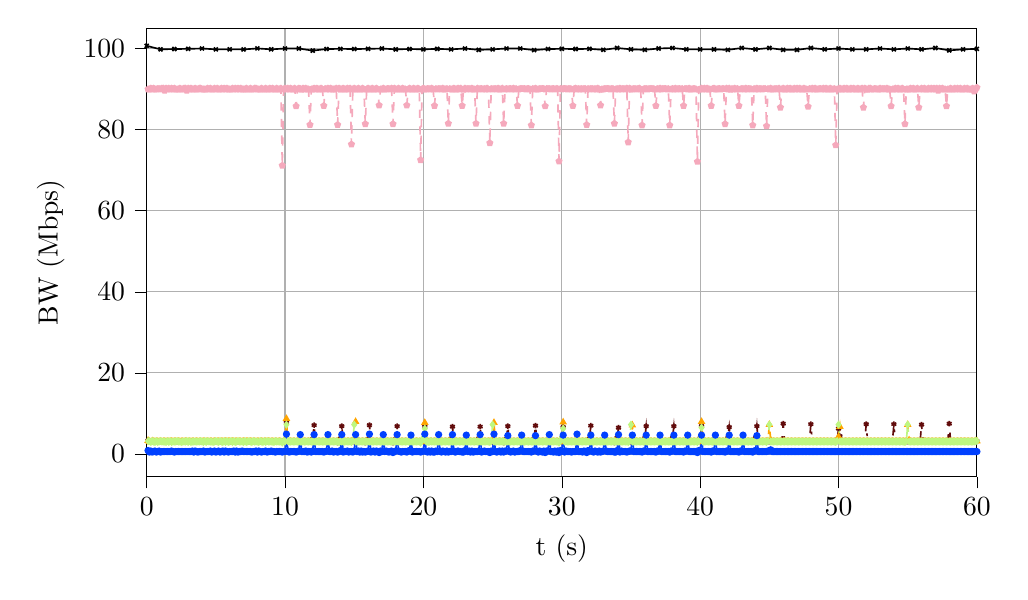
\begin{tikzpicture}

\definecolor{blue064255}{RGB}{0,64,255}
\definecolor{darkgrey176}{RGB}{176,176,176}
\definecolor{lightpink245169188}{RGB}{245,169,188}
\definecolor{maroon971111}{RGB}{97,11,11}
\definecolor{orange}{RGB}{255,165,0}
\definecolor{palegreen190247129}{RGB}{190,247,129}

\begin{axis}[
height=0.6\textwidth,
tick align=outside,
tick pos=left,
width=\textwidth,
x grid style={darkgrey176},
xlabel={t (s)},
xmajorgrids,
xmin=0, xmax=60,
xtick style={color=black},
y grid style={darkgrey176},
ylabel={BW (Mbps)},
ymajorgrids,
ymin=-5.54886786684783, ymax=105,
ytick style={color=black}
]
\addplot [semithick, maroon971111, dash pattern=on 1pt off 3pt on 3pt off 3pt, mark=asterisk, mark size=1, mark options={solid}]
table {%
0.1 3.32258152173913
0.2 3.07182065217391
0.3 3.07182065217391
0.4 3.07182065217391
0.5 3.07182065217391
0.6 3.07182065217391
0.7 3.07182065217391
0.8 3.07182065217391
0.9 3.07182065217391
1 3.07182065217391
1.1 3.07182065217391
1.2 3.07182065217391
1.3 3.07182065217391
1.4 3.07182065217391
1.5 3.07182065217391
1.6 3.07182065217391
1.7 3.07182065217391
1.8 3.07182065217391
1.9 3.07182065217391
2 3.07182065217391
2.1 3.07182065217391
2.2 3.07182065217391
2.3 3.07182065217391
2.4 3.07182065217391
2.5 3.07182065217391
2.6 3.07182065217391
2.7 3.07182065217391
2.8 3.07182065217391
2.9 3.07182065217391
3 3.07182065217391
3.1 3.07182065217391
3.2 3.07182065217391
3.3 3.07182065217391
3.4 3.07182065217391
3.5 3.07182065217391
3.6 3.07182065217391
3.7 3.07182065217391
3.8 3.07182065217391
3.9 3.07182065217391
4 3.07182065217391
4.1 3.07182065217391
4.2 3.07182065217391
4.3 3.07182065217391
4.4 3.07182065217391
4.5 3.07182065217391
4.6 3.07182065217391
4.7 3.07182065217391
4.8 3.07182065217391
4.9 3.07182065217391
5 3.07182065217391
5.1 3.07182065217391
5.2 3.07182065217391
5.3 3.07182065217391
5.4 3.07182065217391
5.5 3.07182065217391
5.6 3.07182065217391
5.7 3.07182065217391
5.8 3.07182065217391
5.9 3.07182065217391
6 3.07182065217391
6.1 3.07182065217391
6.2 3.07182065217391
6.3 3.07182065217391
6.4 3.07182065217391
6.5 3.07182065217391
6.6 3.07182065217391
6.7 3.07182065217391
6.8 3.07182065217391
6.9 3.07182065217391
7 3.07182065217391
7.1 3.07182065217391
7.2 3.07182065217391
7.3 3.07182065217391
7.4 3.07182065217391
7.5 3.07182065217391
7.6 3.07182065217391
7.7 3.07182065217391
7.8 3.07182065217391
7.9 3.07182065217391
8 3.07182065217391
8.1 3.07182065217391
8.2 3.07182065217391
8.3 3.07182065217391
8.4 3.07182065217391
8.5 3.07182065217391
8.6 3.07182065217391
8.7 3.07182065217391
8.8 3.07182065217391
8.9 3.07182065217391
9 3.07182065217391
9.1 3.07182065217391
9.2 3.07182065217391
9.3 3.07182065217391
9.4 3.07182065217391
9.5 3.07182065217391
9.6 3.07182065217391
9.7 3.07182065217391
9.8 2.9464402173913
9.9 3.19720108695652
10 3.07182065217391
10.1 7.86762228260869
10.2 3.07182065217391
10.3 3.07182065217391
10.4 3.07182065217391
10.5 3.07182065217391
10.6 3.07182065217391
10.7 3.07182065217391
10.8 3.07182065217391
10.9 3.07182065217391
11 3.07182065217391
11.1 3.07182065217391
11.2 3.07182065217391
11.3 3.07182065217391
11.4 3.07182065217391
11.5 3.07182065217391
11.6 3.07182065217391
11.7 3.07182065217391
11.8 2.9464402173913
11.9 3.32049184782609
12 3.6861847826087
12.1 7.12578804347826
12.2 3.07182065217391
12.3 3.07182065217391
12.4 3.07182065217391
12.5 3.07182065217391
12.6 3.07182065217391
12.7 3.07182065217391
12.8 3.07182065217391
12.9 3.07182065217391
13 3.07182065217391
13.1 3.07182065217391
13.2 3.07182065217391
13.3 3.07182065217391
13.4 3.07182065217391
13.5 3.07182065217391
13.6 3.07182065217391
13.7 3.07182065217391
13.8 2.8210597826087
13.9 3.32049184782609
14 3.80947554347826
14.1 6.88547554347826
14.2 3.07182065217391
14.3 3.07182065217391
14.4 3.07182065217391
14.5 3.07182065217391
14.6 3.07182065217391
14.7 3.07182065217391
14.8 2.9464402173913
14.9 3.19720108695652
15 3.07182065217391
15.1 3.07182065217391
15.2 3.07182065217391
15.3 3.07182065217391
15.4 3.07182065217391
15.5 3.07182065217391
15.6 3.07182065217391
15.7 3.07182065217391
15.8 2.8210597826087
15.9 3.32049184782609
16 3.6861847826087
16.1 7.12578804347826
16.2 3.07182065217391
16.3 3.07182065217391
16.4 3.07182065217391
16.5 3.07182065217391
16.6 3.07182065217391
16.7 3.07182065217391
16.8 3.07182065217391
16.9 3.07182065217391
17 3.07182065217391
17.1 3.07182065217391
17.2 3.07182065217391
17.3 3.07182065217391
17.4 3.07182065217391
17.5 3.07182065217391
17.6 3.07182065217391
17.7 3.07182065217391
17.8 2.8210597826087
17.9 3.32049184782609
18 3.6861847826087
18.1 6.88547554347826
18.2 3.07182065217391
18.3 3.07182065217391
18.4 3.07182065217391
18.5 3.07182065217391
18.6 3.07182065217391
18.7 3.07182065217391
18.8 3.07182065217391
18.9 3.07182065217391
19 3.07182065217391
19.1 3.07182065217391
19.2 3.07182065217391
19.3 3.07182065217391
19.4 3.07182065217391
19.5 3.07182065217391
19.6 3.07182065217391
19.7 3.07182065217391
19.8 2.9464402173913
19.9 3.32049184782609
20 3.6861847826087
20.1 6.88547554347826
20.2 3.07182065217391
20.3 3.07182065217391
20.4 3.07182065217391
20.5 3.07182065217391
20.6 3.07182065217391
20.7 3.07182065217391
20.8 3.07182065217391
20.9 3.07182065217391
21 3.07182065217391
21.1 3.07182065217391
21.2 3.07182065217391
21.3 3.07182065217391
21.4 3.07182065217391
21.5 3.07182065217391
21.6 3.07182065217391
21.7 3.07182065217391
21.8 2.9464402173913
21.9 3.19511141304348
22 3.80947554347826
22.1 6.76009510869565
22.2 3.07182065217391
22.3 3.07182065217391
22.4 3.07182065217391
22.5 3.07182065217391
22.6 3.07182065217391
22.7 3.07182065217391
22.8 3.07182065217391
22.9 3.07182065217391
23 3.07182065217391
23.1 3.07182065217391
23.2 3.07182065217391
23.3 3.07182065217391
23.4 3.07182065217391
23.5 3.07182065217391
23.6 3.07182065217391
23.7 3.07182065217391
23.8 2.9464402173913
23.9 3.19511141304348
24 3.80947554347826
24.1 6.76009510869565
24.2 3.07182065217391
24.3 3.07182065217391
24.4 3.07182065217391
24.5 3.07182065217391
24.6 3.07182065217391
24.7 3.07182065217391
24.8 3.07182065217391
24.9 3.07182065217391
25 3.07182065217391
25.1 3.07182065217391
25.2 3.07182065217391
25.3 3.07182065217391
25.4 3.07182065217391
25.5 3.07182065217391
25.6 3.07182065217391
25.7 3.07182065217391
25.8 2.8210597826087
25.9 3.32049184782609
26 3.6861847826087
26.1 6.88547554347826
26.2 3.07182065217391
26.3 3.07182065217391
26.4 3.07182065217391
26.5 3.07182065217391
26.6 3.07182065217391
26.7 3.07182065217391
26.8 3.07182065217391
26.9 3.07182065217391
27 3.07182065217391
27.1 3.07182065217391
27.2 3.07182065217391
27.3 3.07182065217391
27.4 3.07182065217391
27.5 3.07182065217391
27.6 3.07182065217391
27.7 3.07182065217391
27.8 3.07182065217391
27.9 3.19511141304348
28 3.80947554347826
28.1 7.00040760869565
28.2 3.07182065217391
28.3 3.07182065217391
28.4 3.07182065217391
28.5 3.07182065217391
28.6 3.07182065217391
28.7 3.07182065217391
28.8 3.07182065217391
28.9 3.07182065217391
29 3.07182065217391
29.1 3.07182065217391
29.2 3.07182065217391
29.3 3.07182065217391
29.4 3.07182065217391
29.5 3.07182065217391
29.6 3.07182065217391
29.7 3.07182065217391
29.8 2.9464402173913
29.9 3.32049184782609
30 3.9317214673913
30.1 6.63471467391304
30.2 3.07182065217391
30.3 3.07182065217391
30.4 3.07182065217391
30.5 3.07182065217391
30.6 3.07182065217391
30.7 3.07182065217391
30.8 3.07182065217391
30.9 3.07182065217391
31 3.07182065217391
31.1 3.07182065217391
31.2 3.07182065217391
31.3 3.07182065217391
31.4 3.07182065217391
31.5 3.07182065217391
31.6 3.07182065217391
31.7 3.07182065217391
31.8 2.9464402173913
31.9 3.19511141304348
32 3.80947554347826
32.1 7.00040760869565
32.2 3.07182065217391
32.3 3.07182065217391
32.4 3.07182065217391
32.5 3.07182065217391
32.6 3.07182065217391
32.7 3.07182065217391
32.8 3.07182065217391
32.9 3.07182065217391
33 3.07182065217391
33.1 3.07182065217391
33.2 3.07182065217391
33.3 3.07182065217391
33.4 3.07182065217391
33.5 3.07182065217391
33.6 3.07182065217391
33.7 3.07182065217391
33.8 2.8210597826087
33.9 3.32049184782609
34 4.05501222826087
34.1 6.50933423913043
34.2 3.07182065217391
34.3 3.07182065217391
34.4 3.07182065217391
34.5 3.07182065217391
34.6 3.07182065217391
34.7 3.07182065217391
34.8 3.07182065217391
34.9 3.07182065217391
35 3.07182065217391
35.1 3.07182065217391
35.2 3.07182065217391
35.3 3.07182065217391
35.4 3.07182065217391
35.5 3.07182065217391
35.6 3.07182065217391
35.7 3.07182065217391
35.8 3.07182065217391
35.9 3.19511141304348
36 3.9317214673913
36.1 6.88547554347826
36.2 3.07182065217391
36.3 3.07182065217391
36.4 3.07182065217391
36.5 3.07182065217391
36.6 3.07182065217391
36.7 3.07182065217391
36.8 3.07182065217391
36.9 3.07182065217391
37 3.07182065217391
37.1 3.07182065217391
37.2 3.07182065217391
37.3 3.07182065217391
37.4 3.07182065217391
37.5 3.07182065217391
37.6 3.07182065217391
37.7 3.07182065217391
37.8 3.07182065217391
37.9 3.19511141304348
38 3.9317214673913
38.1 6.88547554347826
38.2 3.07182065217391
38.3 3.07182065217391
38.4 3.07182065217391
38.5 3.07182065217391
38.6 3.07182065217391
38.7 3.07182065217391
38.8 3.07182065217391
38.9 3.07182065217391
39 3.07182065217391
39.1 3.07182065217391
39.2 3.07182065217391
39.3 3.07182065217391
39.4 3.07182065217391
39.5 3.07182065217391
39.6 3.07182065217391
39.7 3.07182065217391
39.8 2.9464402173913
39.9 3.32049184782609
40 3.9317214673913
40.1 6.88547554347826
40.2 3.07182065217391
40.3 3.07182065217391
40.4 3.07182065217391
40.5 3.07182065217391
40.6 3.07182065217391
40.7 3.07182065217391
40.8 3.07182065217391
40.9 3.07182065217391
41 3.07182065217391
41.1 3.07182065217391
41.2 3.07182065217391
41.3 3.07182065217391
41.4 3.07182065217391
41.5 3.07182065217391
41.6 3.07182065217391
41.7 3.07182065217391
41.8 2.9464402173913
41.9 3.19511141304348
42 3.9317214673913
42.1 6.63471467391304
42.2 3.07182065217391
42.3 3.07182065217391
42.4 3.07182065217391
42.5 3.07182065217391
42.6 3.07182065217391
42.7 3.07182065217391
42.8 3.07182065217391
42.9 3.07182065217391
43 3.07182065217391
43.1 3.07182065217391
43.2 3.07182065217391
43.3 3.07182065217391
43.4 3.07182065217391
43.5 3.07182065217391
43.6 3.07182065217391
43.7 3.07182065217391
43.8 3.07182065217391
43.9 3.19511141304348
44 3.9317214673913
44.1 6.88547554347826
44.2 3.07182065217391
44.3 3.07182065217391
44.4 3.07182065217391
44.5 3.07182065217391
44.6 3.07182065217391
44.7 3.07182065217391
44.8 3.07182065217391
44.9 3.07182065217391
45 3.07182065217391
45.1 3.07182065217391
45.2 3.07182065217391
45.3 2.9464402173913
45.4 3.19720108695652
45.5 3.07182065217391
45.6 3.07182065217391
45.7 3.07182065217391
45.8 2.9464402173913
45.9 3.19511141304348
46 7.49148097826087
46.1 3.07182065217391
46.2 3.07182065217391
46.3 3.07182065217391
46.4 3.07182065217391
46.5 3.07182065217391
46.6 3.07182065217391
46.7 3.07182065217391
46.8 3.07182065217391
46.9 3.07182065217391
47 3.07182065217391
47.1 3.07182065217391
47.2 3.07182065217391
47.3 3.07182065217391
47.4 3.07182065217391
47.5 3.07182065217391
47.6 3.07182065217391
47.7 3.07182065217391
47.8 2.9464402173913
47.9 3.19511141304348
48 7.37654891304348
48.1 3.19511141304348
48.2 3.07182065217391
48.3 3.07182065217391
48.4 3.07182065217391
48.5 3.07182065217391
48.6 3.07182065217391
48.7 3.07182065217391
48.8 3.07182065217391
48.9 3.07182065217391
49 3.07182065217391
49.1 3.07182065217391
49.2 3.07182065217391
49.3 3.07182065217391
49.4 3.07182065217391
49.5 3.07182065217391
49.6 3.07182065217391
49.7 3.07182065217391
49.8 3.07182065217391
49.9 3.19511141304348
50 6.26902173913043
50.1 4.41966032608696
50.2 3.07182065217391
50.3 3.07182065217391
50.4 3.07182065217391
50.5 3.07182065217391
50.6 3.07182065217391
50.7 3.07182065217391
50.8 3.07182065217391
50.9 3.07182065217391
51 3.07182065217391
51.1 3.07182065217391
51.2 3.07182065217391
51.3 3.07182065217391
51.4 3.07182065217391
51.5 3.07182065217391
51.6 3.07182065217391
51.7 3.07182065217391
51.8 2.9464402173913
51.9 3.19511141304348
52 7.37654891304348
52.1 3.19511141304348
52.2 3.07182065217391
52.3 3.07182065217391
52.4 3.07182065217391
52.5 3.07182065217391
52.6 3.07182065217391
52.7 3.07182065217391
52.8 3.07182065217391
52.9 3.07182065217391
53 3.07182065217391
53.1 3.07182065217391
53.2 3.07182065217391
53.3 3.07182065217391
53.4 3.07182065217391
53.5 3.07182065217391
53.6 3.07182065217391
53.7 3.07182065217391
53.8 2.9464402173913
53.9 3.19511141304348
54 7.37654891304348
54.1 3.19511141304348
54.2 3.07182065217391
54.3 3.07182065217391
54.4 3.07182065217391
54.5 3.07182065217391
54.6 3.07182065217391
54.7 3.07182065217391
54.8 3.07182065217391
54.9 3.07182065217391
55 3.07182065217391
55.1 3.07182065217391
55.2 3.07182065217391
55.3 3.07182065217391
55.4 3.07182065217391
55.5 3.07182065217391
55.6 3.07182065217391
55.7 3.07182065217391
55.8 2.9464402173913
55.9 3.19511141304348
56 7.25116847826087
56.1 3.31735733695652
56.2 3.07182065217391
56.3 3.07182065217391
56.4 3.07182065217391
56.5 3.07182065217391
56.6 3.07182065217391
56.7 3.07182065217391
56.8 3.07182065217391
56.9 3.07182065217391
57 3.07182065217391
57.1 3.07182065217391
57.2 3.07182065217391
57.3 3.07182065217391
57.4 3.07182065217391
57.5 3.07182065217391
57.6 3.07182065217391
57.7 3.07182065217391
57.8 2.9464402173913
57.9 3.19511141304348
58 7.49148097826087
58.1 3.07182065217391
58.2 3.07182065217391
58.3 3.07182065217391
58.4 3.07182065217391
58.5 3.07182065217391
58.6 3.07182065217391
58.7 3.07182065217391
58.8 3.07182065217391
58.9 3.07182065217391
59 3.07182065217391
59.1 3.07182065217391
59.2 3.07182065217391
59.3 3.07182065217391
59.4 3.07182065217391
59.5 3.07182065217391
59.6 3.07182065217391
59.7 3.07182065217391
59.8 3.07182065217391
59.9 3.19511141304348
60 3.20138043478261
};
\addplot [semithick, lightpink245169188, dashed, mark=pentagon*, mark size=1, mark options={solid}]
table {%
0.1 89.9604619565217
0.2 89.9604619565217
0.3 90.1694293478261
0.4 89.9604619565217
0.5 90.1694293478261
0.6 89.9604619565217
0.7 89.9604619565217
0.8 90.0649456521739
0.9 90.0649456521739
1 89.9604619565217
1.1 90.1694293478261
1.2 90.1694293478261
1.3 89.6470108695652
1.4 90.1694293478261
1.5 89.9604619565217
1.6 90.1694293478261
1.7 89.9604619565217
1.8 90.1694293478261
1.9 89.9604619565217
2 90.1694293478261
2.1 89.9604619565217
2.2 89.9604619565217
2.3 89.9604619565217
2.4 90.1694293478261
2.5 89.9604619565217
2.6 89.9604619565217
2.7 90.1694293478261
2.8 90.1694293478261
2.9 89.6470108695652
3 90.1694293478261
3.1 89.9604619565217
3.2 90.1694293478261
3.3 89.9604619565217
3.4 89.9604619565217
3.5 90.1694293478261
3.6 89.9604619565217
3.7 89.9604619565217
3.8 90.1694293478261
3.9 90.1694293478261
4 89.9604619565217
4.1 89.9604619565217
4.2 89.9604619565217
4.3 89.9604619565217
4.4 90.1694293478261
4.5 89.9604619565217
4.6 90.1694293478261
4.7 89.9604619565217
4.8 89.9604619565217
4.9 90.1694293478261
5 89.9604619565217
5.1 90.1694293478261
5.2 89.9604619565217
5.3 89.9604619565217
5.4 90.1694293478261
5.5 89.9604619565217
5.6 90.1694293478261
5.7 89.9604619565217
5.8 90.1694293478261
5.9 89.9604619565217
6 89.9604619565217
6.1 89.9604619565217
6.2 90.1694293478261
6.3 89.9604619565217
6.4 90.1694293478261
6.5 89.9604619565217
6.6 90.1694293478261
6.7 89.9604619565217
6.8 90.1694293478261
6.9 89.9604619565217
7 89.9604619565217
7.1 89.9604619565217
7.2 90.1694293478261
7.3 89.9604619565217
7.4 89.9604619565217
7.5 90.1694293478261
7.6 89.9604619565217
7.7 89.9604619565217
7.8 90.1694293478261
7.9 90.1694293478261
8 89.9604619565217
8.1 89.9604619565217
8.2 89.9604619565217
8.3 90.1694293478261
8.4 89.9604619565217
8.5 89.9604619565217
8.6 90.1694293478261
8.7 89.9604619565217
8.8 89.9604619565217
8.9 90.1694293478261
9 89.9604619565217
9.1 90.1694293478261
9.2 89.9604619565217
9.3 89.9604619565217
9.4 90.1694293478261
9.5 89.9604619565217
9.6 89.9604619565217
9.7 90.1694293478261
9.8 71.1533967391304
9.9 89.9604619565217
10 90.1694293478261
10.1 89.9604619565217
10.2 90.1694293478261
10.3 89.9604619565217
10.4 90.1694293478261
10.5 89.9604619565217
10.6 89.9604619565217
10.7 90.1694293478261
10.8 85.7811141304348
10.9 89.9604619565217
11 90.1694293478261
11.1 90.0649456521739
11.2 89.8559782608696
11.3 90.1694293478261
11.4 89.9604619565217
11.5 90.1694293478261
11.6 89.9604619565217
11.7 89.9604619565217
11.8 81.1838315217391
11.9 89.9604619565217
12 89.9604619565217
12.1 90.1694293478261
12.2 89.9604619565217
12.3 90.1694293478261
12.4 89.9604619565217
12.5 89.9604619565217
12.6 90.1694293478261
12.7 89.9604619565217
12.8 85.885597826087
12.9 90.0649456521739
13 89.9604619565217
13.1 90.1694293478261
13.2 89.9604619565217
13.3 90.1694293478261
13.4 89.9604619565217
13.5 89.9604619565217
13.6 89.9604619565217
13.7 90.1694293478261
13.8 81.1838315217391
13.9 90.1694293478261
14 89.9604619565217
14.1 89.9604619565217
14.2 90.1694293478261
14.3 89.9604619565217
14.4 89.9604619565217
14.5 90.1694293478261
14.6 89.9604619565217
14.7 90.1694293478261
14.8 76.3775815217391
14.9 89.9604619565217
15 90.1694293478261
15.1 89.9604619565217
15.2 89.9604619565217
15.3 90.1694293478261
15.4 89.9604619565217
15.5 89.9604619565217
15.6 90.1694293478261
15.7 89.9604619565217
15.8 81.3927989130435
15.9 89.9604619565217
16 90.1694293478261
16.1 89.9604619565217
16.2 89.9604619565217
16.3 90.1694293478261
16.4 89.9604619565217
16.5 89.9604619565217
16.6 90.1694293478261
16.7 89.9604619565217
16.8 85.9900815217391
16.9 89.9604619565217
17 89.9604619565217
17.1 90.1694293478261
17.2 89.9604619565217
17.3 89.9604619565217
17.4 90.0649456521739
17.5 90.0649456521739
17.6 89.9604619565217
17.7 90.1694293478261
17.8 81.3927989130435
17.9 90.1694293478261
18 89.9604619565217
18.1 89.9604619565217
18.2 90.1694293478261
18.3 89.9604619565217
18.4 89.9604619565217
18.5 90.1694293478261
18.6 89.9604619565217
18.7 89.9604619565217
18.8 85.9900815217391
18.9 89.9604619565217
19 90.1694293478261
19.1 89.9604619565217
19.2 89.9604619565217
19.3 90.1694293478261
19.4 89.9604619565217
19.5 89.9604619565217
19.6 90.1694293478261
19.7 89.9604619565217
19.8 72.5116847826087
19.9 89.9604619565217
20 90.1694293478261
20.1 89.9604619565217
20.2 89.9604619565217
20.3 90.0649456521739
20.4 90.0649456521739
20.5 89.9604619565217
20.6 90.1694293478261
20.7 89.9604619565217
20.8 85.885597826087
20.9 90.0649456521739
21 89.9604619565217
21.1 90.0649456521739
21.2 90.0649456521739
21.3 89.9604619565217
21.4 90.1694293478261
21.5 89.9604619565217
21.6 89.9604619565217
21.7 90.0649456521739
21.8 81.4972826086956
21.9 90.0649456521739
22 89.9604619565217
22.1 89.9604619565217
22.2 90.1694293478261
22.3 89.9604619565217
22.4 89.9604619565217
22.5 90.1694293478261
22.6 89.9604619565217
22.7 90.1694293478261
22.8 85.885597826087
22.9 89.8559782608696
23 90.1694293478261
23.1 89.9604619565217
23.2 90.0649456521739
23.3 90.0649456521739
23.4 89.9604619565217
23.5 90.1694293478261
23.6 89.9604619565217
23.7 89.9604619565217
23.8 81.4972826086956
23.9 90.1694293478261
24 89.9604619565217
24.1 90.0649456521739
24.2 90.0649456521739
24.3 89.9604619565217
24.4 90.0649456521739
24.5 89.9604619565217
24.6 90.1694293478261
24.7 89.9604619565217
24.8 76.6910326086957
24.9 90.0649456521739
25 89.9604619565217
25.1 90.0649456521739
25.2 90.0649456521739
25.3 89.9604619565217
25.4 90.1694293478261
25.5 89.9604619565217
25.6 89.9604619565217
25.7 90.1694293478261
25.8 81.4972826086956
25.9 89.9604619565217
26 90.0649456521739
26.1 89.9604619565217
26.2 90.0649456521739
26.3 90.0649456521739
26.4 89.9604619565217
26.5 90.1694293478261
26.6 89.9604619565217
26.7 90.0649456521739
26.8 85.885597826087
26.9 89.9604619565217
27 90.0649456521739
27.1 90.0649456521739
27.2 90.0649456521739
27.3 90.0649456521739
27.4 89.9604619565217
27.5 90.0649456521739
27.6 90.0649456521739
27.7 89.9604619565217
27.8 81.0793478260869
27.9 90.0649456521739
28 89.9604619565217
28.1 90.1694293478261
28.2 89.9604619565217
28.3 89.9604619565217
28.4 90.0649456521739
28.5 90.0649456521739
28.6 90.0649456521739
28.7 90.0649456521739
28.8 85.7811141304348
28.9 90.0649456521739
29 90.0649456521739
29.1 90.0649456521739
29.2 89.9604619565217
29.3 90.0649456521739
29.4 90.0649456521739
29.5 89.9604619565217
29.6 90.0649456521739
29.7 90.0649456521739
29.8 72.1982336956522
29.9 90.0649456521739
30 89.9604619565217
30.1 90.0649456521739
30.2 90.0649456521739
30.3 90.0649456521739
30.4 89.9604619565217
30.5 90.0649456521739
30.6 90.0649456521739
30.7 89.9604619565217
30.8 85.885597826087
30.9 90.0649456521739
31 90.1694293478261
31.1 89.9604619565217
31.2 90.0649456521739
31.3 89.9604619565217
31.4 90.0649456521739
31.5 89.9604619565217
31.6 90.0649456521739
31.7 90.0649456521739
31.8 81.1838315217391
31.9 90.0649456521739
32 89.9604619565217
32.1 90.0649456521739
32.2 90.0649456521739
32.3 89.9604619565217
32.4 90.0649456521739
32.5 89.9604619565217
32.6 90.1694293478261
32.7 89.9604619565217
32.8 85.9900815217391
32.9 89.9604619565217
33 89.9604619565217
33.1 90.0649456521739
33.2 90.0649456521739
33.3 90.0649456521739
33.4 90.0649456521739
33.5 89.9604619565217
33.6 90.0649456521739
33.7 90.0649456521739
33.8 81.4972826086956
33.9 89.9604619565217
34 90.0649456521739
34.1 89.9604619565217
34.2 90.1694293478261
34.3 89.9604619565217
34.4 90.0649456521739
34.5 90.0649456521739
34.6 89.9604619565217
34.7 90.1694293478261
34.8 76.9
34.9 90.1694293478261
35 89.9604619565217
35.1 89.9604619565217
35.2 90.0649456521739
35.3 90.0649456521739
35.4 89.9604619565217
35.5 90.0649456521739
35.6 90.1694293478261
35.7 89.9604619565217
35.8 81.0793478260869
35.9 89.9604619565217
36 90.0649456521739
36.1 90.0649456521739
36.2 89.9604619565217
36.3 90.0649456521739
36.4 90.0649456521739
36.5 90.0649456521739
36.6 90.0649456521739
36.7 89.9604619565217
36.8 85.885597826087
36.9 90.0649456521739
37 89.9604619565217
37.1 90.1694293478261
37.2 89.9604619565217
37.3 90.0649456521739
37.4 90.0649456521739
37.5 90.0649456521739
37.6 89.9604619565217
37.7 90.0649456521739
37.8 81.0793478260869
37.9 89.9604619565217
38 90.0649456521739
38.1 89.9604619565217
38.2 90.1694293478261
38.3 89.9604619565217
38.4 90.0649456521739
38.5 90.0649456521739
38.6 89.9604619565217
38.7 90.0649456521739
38.8 85.885597826087
38.9 90.0649456521739
39 90.0649456521739
39.1 89.9604619565217
39.2 90.1694293478261
39.3 89.9604619565217
39.4 89.9604619565217
39.5 90.0649456521739
39.6 90.0649456521739
39.7 89.9604619565217
39.8 72.09375
39.9 89.8559782608696
40 89.9604619565217
40.1 90.1694293478261
40.2 89.9604619565217
40.3 90.1694293478261
40.4 89.9604619565217
40.5 90.1694293478261
40.6 89.9604619565217
40.7 89.9604619565217
40.8 85.885597826087
40.9 90.0649456521739
41 90.1694293478261
41.1 89.9604619565217
41.2 89.9604619565217
41.3 90.0649456521739
41.4 90.0649456521739
41.5 89.9604619565217
41.6 90.0649456521739
41.7 90.0649456521739
41.8 81.3927989130435
41.9 90.1694293478261
42 89.9604619565217
42.1 90.1694293478261
42.2 89.8559782608696
42.3 90.0649456521739
42.4 89.9604619565217
42.5 90.1694293478261
42.6 89.9604619565217
42.7 90.0649456521739
42.8 85.885597826087
42.9 89.9604619565217
43 90.0649456521739
43.1 90.0649456521739
43.2 89.9604619565217
43.3 90.1694293478261
43.4 89.9604619565217
43.5 90.0649456521739
43.6 90.0649456521739
43.7 89.9604619565217
43.8 81.0793478260869
43.9 90.0649456521739
44 89.9604619565217
44.1 90.1694293478261
44.2 89.9604619565217
44.3 90.0649456521739
44.4 90.0649456521739
44.5 89.9604619565217
44.6 90.0649456521739
44.7 90.0649456521739
44.8 80.8703804347826
44.9 90.0649456521739
45 89.9604619565217
45.1 90.1694293478261
45.2 89.9604619565217
45.3 89.9604619565217
45.4 90.0649456521739
45.5 90.0649456521739
45.6 89.9604619565217
45.7 90.1694293478261
45.8 85.4676630434783
45.9 89.9604619565217
46 90.1694293478261
46.1 89.9604619565217
46.2 89.9604619565217
46.3 90.1694293478261
46.4 89.9604619565217
46.5 90.1694293478261
46.6 89.9604619565217
46.7 89.9604619565217
46.8 90.1694293478261
46.9 89.9604619565217
47 90.1694293478261
47.1 89.9604619565217
47.2 90.1694293478261
47.3 89.9604619565217
47.4 89.9604619565217
47.5 90.1694293478261
47.6 89.9604619565217
47.7 89.9604619565217
47.8 85.6766304347826
47.9 90.0649456521739
48 89.9604619565217
48.1 90.1694293478261
48.2 89.9604619565217
48.3 90.1694293478261
48.4 89.9604619565217
48.5 89.9604619565217
48.6 90.0649456521739
48.7 90.0649456521739
48.8 89.9604619565217
48.9 90.1694293478261
49 89.9604619565217
49.1 90.1694293478261
49.2 89.9604619565217
49.3 89.9604619565217
49.4 90.1694293478261
49.5 89.9604619565217
49.6 89.9604619565217
49.7 90.0649456521739
49.8 76.1686141304348
49.9 89.9604619565217
50 89.9604619565217
50.1 90.1694293478261
50.2 89.9604619565217
50.3 89.9604619565217
50.4 90.1694293478261
50.5 89.9604619565217
50.6 90.1694293478261
50.7 89.9604619565217
50.8 89.9604619565217
50.9 90.1694293478261
51 89.9604619565217
51.1 90.1694293478261
51.2 89.9604619565217
51.3 89.9604619565217
51.4 90.1694293478261
51.5 89.9604619565217
51.6 89.9604619565217
51.7 90.1694293478261
51.8 85.4676630434783
51.9 90.1694293478261
52 89.9604619565217
52.1 89.8559782608696
52.2 90.1694293478261
52.3 90.1694293478261
52.4 89.9604619565217
52.5 89.9604619565217
52.6 90.0649456521739
52.7 90.0649456521739
52.8 89.9604619565217
52.9 89.9604619565217
53 90.1694293478261
53.1 89.9604619565217
53.2 90.0649456521739
53.3 90.0649456521739
53.4 89.9604619565217
53.5 90.1694293478261
53.6 89.9604619565217
53.7 89.9604619565217
53.8 85.7811141304348
53.9 89.9604619565217
54 89.9604619565217
54.1 90.1694293478261
54.2 89.9604619565217
54.3 90.1694293478261
54.4 89.9604619565217
54.5 89.9604619565217
54.6 90.1694293478261
54.7 89.9604619565217
54.8 81.3927989130435
54.9 89.9604619565217
55 89.9604619565217
55.1 89.9604619565217
55.2 90.1694293478261
55.3 89.9604619565217
55.4 90.1694293478261
55.5 89.9604619565217
55.6 89.9604619565217
55.7 90.1694293478261
55.8 85.4676630434783
55.9 89.9604619565217
56 90.1694293478261
56.1 89.9604619565217
56.2 90.1694293478261
56.3 89.9604619565217
56.4 89.9604619565217
56.5 90.1694293478261
56.6 89.9604619565217
56.7 90.1694293478261
56.8 89.9604619565217
56.9 90.1694293478261
57 89.9604619565217
57.1 90.1694293478261
57.2 89.6470108695652
57.3 90.1694293478261
57.4 89.9604619565217
57.5 90.1694293478261
57.6 89.9604619565217
57.7 89.9604619565217
57.8 85.7811141304348
57.9 89.9604619565217
58 89.9604619565217
58.1 90.1694293478261
58.2 89.9604619565217
58.3 89.9604619565217
58.4 90.1694293478261
58.5 89.9604619565217
58.6 90.1694293478261
58.7 89.9604619565217
58.8 90.1694293478261
58.9 89.9604619565217
59 89.9604619565217
59.1 90.1694293478261
59.2 89.9604619565217
59.3 90.1694293478261
59.4 89.9604619565217
59.5 89.9604619565217
59.6 89.9604619565217
59.7 90.1694293478261
59.8 89.4380434782609
59.9 89.8559782608696
60 90.3783967391304
};
\addplot [semithick, orange, dashed, mark=triangle*, mark size=1, mark options={solid}]
table {%
0.1 3.32258152173913
0.2 3.07182065217391
0.3 2.9464402173913
0.4 3.19720108695652
0.5 3.07182065217391
0.6 3.07182065217391
0.7 3.07182065217391
0.8 3.07182065217391
0.9 3.07182065217391
1 3.07182065217391
1.1 3.07182065217391
1.2 3.07182065217391
1.3 3.07182065217391
1.4 3.07182065217391
1.5 3.07182065217391
1.6 3.07182065217391
1.7 3.07182065217391
1.8 3.07182065217391
1.9 3.07182065217391
2 3.07182065217391
2.1 3.07182065217391
2.2 3.07182065217391
2.3 3.07182065217391
2.4 3.07182065217391
2.5 3.07182065217391
2.6 3.07182065217391
2.7 3.07182065217391
2.8 3.07182065217391
2.9 3.07182065217391
3 3.07182065217391
3.1 3.07182065217391
3.2 3.07182065217391
3.3 3.07182065217391
3.4 3.07182065217391
3.5 3.07182065217391
3.6 3.07182065217391
3.7 3.07182065217391
3.8 3.07182065217391
3.9 3.07182065217391
4 3.07182065217391
4.1 3.07182065217391
4.2 3.07182065217391
4.3 3.07182065217391
4.4 3.07182065217391
4.5 3.07182065217391
4.6 3.07182065217391
4.7 3.07182065217391
4.8 3.07182065217391
4.9 3.07182065217391
5 3.07182065217391
5.1 3.07182065217391
5.2 3.07182065217391
5.3 3.07182065217391
5.4 3.07182065217391
5.5 3.07182065217391
5.6 3.07182065217391
5.7 3.07182065217391
5.8 3.07182065217391
5.9 3.07182065217391
6 3.07182065217391
6.1 3.07182065217391
6.2 3.07182065217391
6.3 3.07182065217391
6.4 3.07182065217391
6.5 3.07182065217391
6.6 3.07182065217391
6.7 3.07182065217391
6.8 3.07182065217391
6.9 3.07182065217391
7 3.07182065217391
7.1 3.07182065217391
7.2 3.07182065217391
7.3 3.07182065217391
7.4 3.07182065217391
7.5 3.07182065217391
7.6 3.07182065217391
7.7 3.07182065217391
7.8 3.07182065217391
7.9 3.07182065217391
8 3.07182065217391
8.1 3.07182065217391
8.2 3.07182065217391
8.3 3.07182065217391
8.4 3.07182065217391
8.5 3.07182065217391
8.6 3.07182065217391
8.7 3.07182065217391
8.8 3.07182065217391
8.9 3.07182065217391
9 3.07182065217391
9.1 3.07182065217391
9.2 3.07182065217391
9.3 3.07182065217391
9.4 3.07182065217391
9.5 3.07182065217391
9.6 3.07182065217391
9.7 3.07182065217391
9.8 2.9464402173913
9.9 3.19720108695652
10 3.07182065217391
10.1 8.72438858695652
10.2 3.07182065217391
10.3 3.07182065217391
10.4 3.07182065217391
10.5 3.07182065217391
10.6 3.07182065217391
10.7 3.07182065217391
10.8 3.07182065217391
10.9 3.07182065217391
11 3.07182065217391
11.1 3.07182065217391
11.2 3.07182065217391
11.3 3.07182065217391
11.4 3.07182065217391
11.5 3.07182065217391
11.6 3.07182065217391
11.7 3.07182065217391
11.8 3.07182065217391
11.9 3.07182065217391
12 3.07182065217391
12.1 3.07182065217391
12.2 3.07182065217391
12.3 3.07182065217391
12.4 3.07182065217391
12.5 3.07182065217391
12.6 3.07182065217391
12.7 3.07182065217391
12.8 3.07182065217391
12.9 3.07182065217391
13 3.07182065217391
13.1 3.07182065217391
13.2 3.07182065217391
13.3 3.07182065217391
13.4 3.07182065217391
13.5 3.07182065217391
13.6 3.07182065217391
13.7 3.07182065217391
13.8 3.07182065217391
13.9 3.07182065217391
14 3.07182065217391
14.1 3.07182065217391
14.2 3.07182065217391
14.3 3.07182065217391
14.4 3.07182065217391
14.5 3.07182065217391
14.6 3.07182065217391
14.7 3.07182065217391
14.8 3.07182065217391
14.9 3.19511141304348
15 3.19511141304348
15.1 7.98255434782609
15.2 3.07182065217391
15.3 3.07182065217391
15.4 3.07182065217391
15.5 3.07182065217391
15.6 3.07182065217391
15.7 3.07182065217391
15.8 3.07182065217391
15.9 3.07182065217391
16 3.07182065217391
16.1 3.07182065217391
16.2 3.07182065217391
16.3 3.07182065217391
16.4 3.07182065217391
16.5 3.07182065217391
16.6 3.07182065217391
16.7 3.07182065217391
16.8 3.07182065217391
16.9 3.07182065217391
17 3.07182065217391
17.1 3.07182065217391
17.2 3.07182065217391
17.3 3.07182065217391
17.4 3.07182065217391
17.5 3.07182065217391
17.6 3.07182065217391
17.7 3.07182065217391
17.8 3.07182065217391
17.9 3.07182065217391
18 3.07182065217391
18.1 3.07182065217391
18.2 3.07182065217391
18.3 3.07182065217391
18.4 3.07182065217391
18.5 3.07182065217391
18.6 3.07182065217391
18.7 3.07182065217391
18.8 3.07182065217391
18.9 3.07182065217391
19 3.07182065217391
19.1 3.07182065217391
19.2 3.07182065217391
19.3 3.07182065217391
19.4 3.07182065217391
19.5 3.07182065217391
19.6 3.07182065217391
19.7 3.07182065217391
19.8 2.9464402173913
19.9 3.19720108695652
20 3.19511141304348
20.1 7.74224184782609
20.2 3.07182065217391
20.3 3.07182065217391
20.4 3.07182065217391
20.5 3.07182065217391
20.6 3.07182065217391
20.7 3.07182065217391
20.8 3.07182065217391
20.9 3.07182065217391
21 3.07182065217391
21.1 3.07182065217391
21.2 3.07182065217391
21.3 3.07182065217391
21.4 3.07182065217391
21.5 3.07182065217391
21.6 3.07182065217391
21.7 3.07182065217391
21.8 3.07182065217391
21.9 3.07182065217391
22 3.07182065217391
22.1 3.07182065217391
22.2 3.07182065217391
22.3 3.07182065217391
22.4 3.07182065217391
22.5 3.07182065217391
22.6 3.07182065217391
22.7 3.07182065217391
22.8 3.07182065217391
22.9 3.07182065217391
23 3.07182065217391
23.1 3.07182065217391
23.2 3.07182065217391
23.3 3.07182065217391
23.4 3.07182065217391
23.5 3.07182065217391
23.6 3.07182065217391
23.7 3.07182065217391
23.8 3.07182065217391
23.9 3.07182065217391
24 3.07182065217391
24.1 3.07182065217391
24.2 3.07182065217391
24.3 3.07182065217391
24.4 3.07182065217391
24.5 3.07182065217391
24.6 3.07182065217391
24.7 3.07182065217391
24.8 3.07182065217391
24.9 3.19511141304348
25 3.31735733695652
25.1 7.74224184782609
25.2 3.07182065217391
25.3 3.07182065217391
25.4 3.07182065217391
25.5 3.07182065217391
25.6 3.07182065217391
25.7 3.07182065217391
25.8 3.07182065217391
25.9 3.07182065217391
26 3.07182065217391
26.1 3.07182065217391
26.2 3.07182065217391
26.3 3.07182065217391
26.4 3.07182065217391
26.5 3.07182065217391
26.6 3.07182065217391
26.7 3.07182065217391
26.8 3.07182065217391
26.9 3.07182065217391
27 3.07182065217391
27.1 3.07182065217391
27.2 3.07182065217391
27.3 3.07182065217391
27.4 3.07182065217391
27.5 3.07182065217391
27.6 3.07182065217391
27.7 3.07182065217391
27.8 3.07182065217391
27.9 3.07182065217391
28 3.07182065217391
28.1 3.07182065217391
28.2 3.07182065217391
28.3 3.07182065217391
28.4 3.07182065217391
28.5 3.07182065217391
28.6 3.07182065217391
28.7 3.07182065217391
28.8 3.07182065217391
28.9 3.07182065217391
29 3.07182065217391
29.1 3.07182065217391
29.2 3.07182065217391
29.3 3.07182065217391
29.4 3.07182065217391
29.5 3.07182065217391
29.6 3.07182065217391
29.7 3.07182065217391
29.8 2.9464402173913
29.9 3.19720108695652
30 3.19511141304348
30.1 7.86762228260869
30.2 3.07182065217391
30.3 3.07182065217391
30.4 3.07182065217391
30.5 3.07182065217391
30.6 3.07182065217391
30.7 3.07182065217391
30.8 3.07182065217391
30.9 3.07182065217391
31 3.07182065217391
31.1 3.07182065217391
31.2 3.07182065217391
31.3 3.07182065217391
31.4 3.07182065217391
31.5 3.07182065217391
31.6 3.07182065217391
31.7 3.07182065217391
31.8 3.07182065217391
31.9 3.07182065217391
32 3.07182065217391
32.1 3.07182065217391
32.2 3.07182065217391
32.3 3.07182065217391
32.4 3.07182065217391
32.5 3.07182065217391
32.6 3.07182065217391
32.7 3.07182065217391
32.8 3.07182065217391
32.9 3.07182065217391
33 3.07182065217391
33.1 3.07182065217391
33.2 3.07182065217391
33.3 3.07182065217391
33.4 3.07182065217391
33.5 3.07182065217391
33.6 3.07182065217391
33.7 3.07182065217391
33.8 3.07182065217391
33.9 3.07182065217391
34 3.07182065217391
34.1 3.07182065217391
34.2 3.07182065217391
34.3 3.07182065217391
34.4 3.07182065217391
34.5 3.07182065217391
34.6 3.07182065217391
34.7 3.07182065217391
34.8 3.07182065217391
34.9 3.19511141304348
35 3.56289402173913
35.1 7.12578804347826
35.2 3.07182065217391
35.3 3.07182065217391
35.4 3.07182065217391
35.5 3.07182065217391
35.6 3.07182065217391
35.7 3.07182065217391
35.8 3.07182065217391
35.9 3.07182065217391
36 3.07182065217391
36.1 3.07182065217391
36.2 3.07182065217391
36.3 3.07182065217391
36.4 3.07182065217391
36.5 3.07182065217391
36.6 3.07182065217391
36.7 3.07182065217391
36.8 3.07182065217391
36.9 3.07182065217391
37 3.07182065217391
37.1 3.07182065217391
37.2 3.07182065217391
37.3 3.07182065217391
37.4 3.07182065217391
37.5 3.07182065217391
37.6 3.07182065217391
37.7 3.07182065217391
37.8 3.07182065217391
37.9 3.07182065217391
38 3.07182065217391
38.1 3.07182065217391
38.2 3.07182065217391
38.3 3.07182065217391
38.4 3.07182065217391
38.5 3.07182065217391
38.6 3.07182065217391
38.7 3.07182065217391
38.8 3.07182065217391
38.9 3.07182065217391
39 3.07182065217391
39.1 3.07182065217391
39.2 3.07182065217391
39.3 3.07182065217391
39.4 3.07182065217391
39.5 3.07182065217391
39.6 3.07182065217391
39.7 3.07182065217391
39.8 2.9464402173913
39.9 3.19720108695652
40 3.19511141304348
40.1 7.98255434782609
40.2 3.07182065217391
40.3 3.07182065217391
40.4 3.07182065217391
40.5 3.07182065217391
40.6 3.07182065217391
40.7 3.07182065217391
40.8 3.07182065217391
40.9 3.07182065217391
41 3.07182065217391
41.1 3.07182065217391
41.2 3.07182065217391
41.3 3.07182065217391
41.4 3.07182065217391
41.5 3.07182065217391
41.6 3.07182065217391
41.7 3.07182065217391
41.8 3.07182065217391
41.9 3.07182065217391
42 3.07182065217391
42.1 3.07182065217391
42.2 3.07182065217391
42.3 3.07182065217391
42.4 3.07182065217391
42.5 3.07182065217391
42.6 3.07182065217391
42.7 3.07182065217391
42.8 3.07182065217391
42.9 3.07182065217391
43 3.07182065217391
43.1 3.07182065217391
43.2 3.07182065217391
43.3 3.07182065217391
43.4 3.07182065217391
43.5 3.07182065217391
43.6 3.07182065217391
43.7 3.07182065217391
43.8 3.07182065217391
43.9 3.07182065217391
44 3.07182065217391
44.1 3.07182065217391
44.2 3.07182065217391
44.3 3.07182065217391
44.4 3.07182065217391
44.5 3.07182065217391
44.6 3.07182065217391
44.7 3.07182065217391
44.8 3.07182065217391
44.9 3.19511141304348
45 7.25116847826087
45.1 3.44064809782609
45.2 3.07182065217391
45.3 3.07182065217391
45.4 3.07182065217391
45.5 3.07182065217391
45.6 3.07182065217391
45.7 3.07182065217391
45.8 3.07182065217391
45.9 3.07182065217391
46 3.07182065217391
46.1 3.07182065217391
46.2 3.07182065217391
46.3 3.07182065217391
46.4 3.07182065217391
46.5 3.07182065217391
46.6 3.07182065217391
46.7 3.07182065217391
46.8 3.07182065217391
46.9 3.07182065217391
47 3.07182065217391
47.1 3.07182065217391
47.2 3.07182065217391
47.3 3.07182065217391
47.4 3.07182065217391
47.5 3.07182065217391
47.6 3.07182065217391
47.7 3.07182065217391
47.8 3.07182065217391
47.9 3.07182065217391
48 3.07182065217391
48.1 3.07182065217391
48.2 3.07182065217391
48.3 3.07182065217391
48.4 3.07182065217391
48.5 3.07182065217391
48.6 3.07182065217391
48.7 3.07182065217391
48.8 3.07182065217391
48.9 3.07182065217391
49 3.07182065217391
49.1 3.07182065217391
49.2 3.07182065217391
49.3 3.07182065217391
49.4 3.07182065217391
49.5 3.07182065217391
49.6 3.07182065217391
49.7 3.07182065217391
49.8 3.07182065217391
49.9 3.19511141304348
50 4.30472826086956
50.1 6.76009510869565
50.2 3.07182065217391
50.3 3.07182065217391
50.4 3.07182065217391
50.5 3.07182065217391
50.6 3.07182065217391
50.7 3.07182065217391
50.8 3.07182065217391
50.9 3.07182065217391
51 3.07182065217391
51.1 3.07182065217391
51.2 3.07182065217391
51.3 3.07182065217391
51.4 3.07182065217391
51.5 3.07182065217391
51.6 3.07182065217391
51.7 3.07182065217391
51.8 3.07182065217391
51.9 3.07182065217391
52 3.07182065217391
52.1 3.07182065217391
52.2 3.07182065217391
52.3 3.07182065217391
52.4 3.07182065217391
52.5 3.07182065217391
52.6 3.07182065217391
52.7 3.07182065217391
52.8 3.07182065217391
52.9 3.07182065217391
53 3.07182065217391
53.1 3.07182065217391
53.2 3.07182065217391
53.3 3.07182065217391
53.4 3.07182065217391
53.5 3.07182065217391
53.6 3.07182065217391
53.7 3.07182065217391
53.8 3.07182065217391
53.9 3.07182065217391
54 3.07182065217391
54.1 3.07182065217391
54.2 3.07182065217391
54.3 3.07182065217391
54.4 3.07182065217391
54.5 3.07182065217391
54.6 3.07182065217391
54.7 3.07182065217391
54.8 3.07182065217391
54.9 3.19511141304348
55 7.25116847826087
55.1 3.44064809782609
55.2 3.07182065217391
55.3 3.07182065217391
55.4 3.07182065217391
55.5 3.07182065217391
55.6 3.07182065217391
55.7 3.07182065217391
55.8 3.07182065217391
55.9 3.07182065217391
56 3.07182065217391
56.1 3.07182065217391
56.2 3.07182065217391
56.3 3.07182065217391
56.4 3.07182065217391
56.5 3.07182065217391
56.6 3.07182065217391
56.7 3.07182065217391
56.8 3.07182065217391
56.9 3.07182065217391
57 3.07182065217391
57.1 3.07182065217391
57.2 3.07182065217391
57.3 3.07182065217391
57.4 3.07182065217391
57.5 3.07182065217391
57.6 3.07182065217391
57.7 3.07182065217391
57.8 3.07182065217391
57.9 3.07182065217391
58 3.07182065217391
58.1 3.07182065217391
58.2 3.07182065217391
58.3 3.07182065217391
58.4 3.07182065217391
58.5 3.07182065217391
58.6 3.07182065217391
58.7 3.07182065217391
58.8 3.07182065217391
58.9 3.07182065217391
59 3.07182065217391
59.1 3.07182065217391
59.2 3.07182065217391
59.3 3.07182065217391
59.4 3.07182065217391
59.5 3.07182065217391
59.6 3.07182065217391
59.7 3.07182065217391
59.8 3.07182065217391
59.9 3.19511141304348
60 3.20033559782609
};
\addplot [semithick, palegreen190247129, dash pattern=on 1pt off 3pt on 3pt off 3pt, mark=diamond*, mark size=1, mark options={solid}]
table {%
0.1 3.19720108695652
0.2 3.19720108695652
0.3 2.9464402173913
0.4 3.19720108695652
0.5 3.07182065217391
0.6 2.9464402173913
0.7 3.19720108695652
0.8 2.9464402173913
0.9 3.07182065217391
1 3.19720108695652
1.1 3.07182065217391
1.2 3.07182065217391
1.3 3.07182065217391
1.4 2.9464402173913
1.5 3.19720108695652
1.6 2.9464402173913
1.7 3.19720108695652
1.8 2.9464402173913
1.9 3.07182065217391
2 3.07182065217391
2.1 3.07182065217391
2.2 3.19720108695652
2.3 3.07182065217391
2.4 3.07182065217391
2.5 2.9464402173913
2.6 3.07182065217391
2.7 3.07182065217391
2.8 3.07182065217391
2.9 3.19720108695652
3 2.9464402173913
3.1 3.19720108695652
3.2 2.9464402173913
3.3 3.07182065217391
3.4 3.07182065217391
3.5 3.07182065217391
3.6 3.07182065217391
3.7 3.07182065217391
3.8 3.07182065217391
3.9 3.19720108695652
4 3.07182065217391
4.1 2.9464402173913
4.2 3.19720108695652
4.3 2.9464402173913
4.4 3.19720108695652
4.5 3.07182065217391
4.6 3.07182065217391
4.7 3.07182065217391
4.8 2.9464402173913
4.9 3.07182065217391
5 3.19720108695652
5.1 3.07182065217391
5.2 2.9464402173913
5.3 3.19720108695652
5.4 3.07182065217391
5.5 2.9464402173913
5.6 3.19720108695652
5.7 2.9464402173913
5.8 3.19720108695652
5.9 2.9464402173913
6 3.07182065217391
6.1 3.19720108695652
6.2 2.9464402173913
6.3 3.19720108695652
6.4 2.9464402173913
6.5 3.07182065217391
6.6 3.19720108695652
6.7 3.07182065217391
6.8 3.07182065217391
6.9 3.07182065217391
7 2.9464402173913
7.1 3.19720108695652
7.2 2.9464402173913
7.3 3.07182065217391
7.4 3.19720108695652
7.5 3.07182065217391
7.6 2.9464402173913
7.7 3.19720108695652
7.8 3.07182065217391
7.9 3.07182065217391
8 3.07182065217391
8.1 2.9464402173913
8.2 3.19720108695652
8.3 3.07182065217391
8.4 2.9464402173913
8.5 3.19720108695652
8.6 2.9464402173913
8.7 3.19720108695652
8.8 3.07182065217391
8.9 3.07182065217391
9 3.07182065217391
9.1 3.07182065217391
9.2 2.9464402173913
9.3 3.19720108695652
9.4 3.07182065217391
9.5 3.07182065217391
9.6 3.07182065217391
9.7 3.07182065217391
9.8 2.8210597826087
9.9 3.19720108695652
10 3.07182065217391
10.1 7.25116847826087
10.2 3.19720108695652
10.3 3.07182065217391
10.4 3.07182065217391
10.5 3.07182065217391
10.6 3.07182065217391
10.7 3.07182065217391
10.8 3.07182065217391
10.9 3.07182065217391
11 3.07182065217391
11.1 3.07182065217391
11.2 3.07182065217391
11.3 3.07182065217391
11.4 3.07182065217391
11.5 3.07182065217391
11.6 3.07182065217391
11.7 3.07182065217391
11.8 3.07182065217391
11.9 3.07182065217391
12 3.07182065217391
12.1 3.07182065217391
12.2 3.07182065217391
12.3 3.07182065217391
12.4 3.07182065217391
12.5 3.07182065217391
12.6 3.07182065217391
12.7 3.07182065217391
12.8 3.07182065217391
12.9 3.07182065217391
13 3.07182065217391
13.1 3.07182065217391
13.2 3.07182065217391
13.3 3.07182065217391
13.4 3.07182065217391
13.5 3.07182065217391
13.6 3.07182065217391
13.7 3.07182065217391
13.8 3.07182065217391
13.9 2.9464402173913
14 3.19720108695652
14.1 3.07182065217391
14.2 3.07182065217391
14.3 3.07182065217391
14.4 3.07182065217391
14.5 3.07182065217391
14.6 3.07182065217391
14.7 3.07182065217391
14.8 2.9464402173913
14.9 3.19511141304348
15 7.25116847826087
15.1 3.07182065217391
15.2 3.07182065217391
15.3 3.07182065217391
15.4 3.07182065217391
15.5 3.07182065217391
15.6 3.07182065217391
15.7 3.07182065217391
15.8 3.07182065217391
15.9 3.07182065217391
16 3.07182065217391
16.1 3.07182065217391
16.2 3.07182065217391
16.3 3.07182065217391
16.4 3.07182065217391
16.5 3.07182065217391
16.6 3.07182065217391
16.7 3.07182065217391
16.8 3.07182065217391
16.9 3.07182065217391
17 3.07182065217391
17.1 3.07182065217391
17.2 3.07182065217391
17.3 3.07182065217391
17.4 3.07182065217391
17.5 3.07182065217391
17.6 3.07182065217391
17.7 3.07182065217391
17.8 3.07182065217391
17.9 3.07182065217391
18 3.07182065217391
18.1 3.07182065217391
18.2 3.07182065217391
18.3 3.07182065217391
18.4 3.07182065217391
18.5 3.07182065217391
18.6 3.07182065217391
18.7 3.07182065217391
18.8 3.07182065217391
18.9 3.07182065217391
19 3.07182065217391
19.1 3.07182065217391
19.2 3.07182065217391
19.3 3.07182065217391
19.4 3.07182065217391
19.5 3.07182065217391
19.6 3.07182065217391
19.7 3.07182065217391
19.8 2.8210597826087
19.9 3.32049184782609
20 4.05501222826087
20.1 6.26902173913043
20.2 3.07182065217391
20.3 3.07182065217391
20.4 2.9464402173913
20.5 3.19720108695652
20.6 3.07182065217391
20.7 3.07182065217391
20.8 3.07182065217391
20.9 3.07182065217391
21 3.07182065217391
21.1 3.07182065217391
21.2 3.07182065217391
21.3 3.07182065217391
21.4 3.07182065217391
21.5 3.07182065217391
21.6 3.07182065217391
21.7 3.07182065217391
21.8 3.07182065217391
21.9 3.07182065217391
22 3.07182065217391
22.1 3.07182065217391
22.2 3.07182065217391
22.3 3.07182065217391
22.4 3.07182065217391
22.5 3.07182065217391
22.6 3.07182065217391
22.7 3.07182065217391
22.8 3.07182065217391
22.9 3.07182065217391
23 3.07182065217391
23.1 3.07182065217391
23.2 3.07182065217391
23.3 3.07182065217391
23.4 3.07182065217391
23.5 3.07182065217391
23.6 3.07182065217391
23.7 3.07182065217391
23.8 3.07182065217391
23.9 3.07182065217391
24 3.07182065217391
24.1 3.07182065217391
24.2 3.07182065217391
24.3 3.07182065217391
24.4 3.07182065217391
24.5 3.07182065217391
24.6 3.07182065217391
24.7 3.07182065217391
24.8 2.9464402173913
24.9 3.19511141304348
25 7.25116847826087
25.1 3.07182065217391
25.2 3.07182065217391
25.3 3.07182065217391
25.4 3.07182065217391
25.5 3.07182065217391
25.6 3.07182065217391
25.7 3.07182065217391
25.8 3.07182065217391
25.9 3.07182065217391
26 3.07182065217391
26.1 3.07182065217391
26.2 3.07182065217391
26.3 3.07182065217391
26.4 3.07182065217391
26.5 3.07182065217391
26.6 3.07182065217391
26.7 3.07182065217391
26.8 3.07182065217391
26.9 3.07182065217391
27 3.07182065217391
27.1 3.07182065217391
27.2 3.07182065217391
27.3 3.07182065217391
27.4 3.07182065217391
27.5 3.07182065217391
27.6 3.07182065217391
27.7 3.07182065217391
27.8 3.07182065217391
27.9 3.07182065217391
28 3.07182065217391
28.1 3.07182065217391
28.2 3.07182065217391
28.3 3.07182065217391
28.4 3.07182065217391
28.5 3.07182065217391
28.6 3.07182065217391
28.7 3.07182065217391
28.8 3.07182065217391
28.9 3.07182065217391
29 3.07182065217391
29.1 3.07182065217391
29.2 3.07182065217391
29.3 3.07182065217391
29.4 3.07182065217391
29.5 3.07182065217391
29.6 3.07182065217391
29.7 3.07182065217391
29.8 2.8210597826087
29.9 3.32049184782609
30 4.05501222826087
30.1 6.26902173913043
30.2 3.07182065217391
30.3 3.07182065217391
30.4 3.07182065217391
30.5 3.07182065217391
30.6 3.07182065217391
30.7 3.07182065217391
30.8 3.07182065217391
30.9 3.07182065217391
31 3.07182065217391
31.1 3.07182065217391
31.2 3.07182065217391
31.3 3.07182065217391
31.4 3.07182065217391
31.5 3.07182065217391
31.6 3.07182065217391
31.7 3.07182065217391
31.8 3.07182065217391
31.9 3.07182065217391
32 3.07182065217391
32.1 3.07182065217391
32.2 3.07182065217391
32.3 3.07182065217391
32.4 3.07182065217391
32.5 3.07182065217391
32.6 3.07182065217391
32.7 3.07182065217391
32.8 3.07182065217391
32.9 3.07182065217391
33 3.07182065217391
33.1 3.07182065217391
33.2 3.07182065217391
33.3 3.07182065217391
33.4 3.07182065217391
33.5 3.07182065217391
33.6 3.07182065217391
33.7 3.07182065217391
33.8 3.07182065217391
33.9 3.07182065217391
34 3.07182065217391
34.1 3.07182065217391
34.2 3.07182065217391
34.3 3.07182065217391
34.4 3.07182065217391
34.5 3.07182065217391
34.6 3.07182065217391
34.7 3.07182065217391
34.8 2.9464402173913
34.9 3.19511141304348
35 7.25116847826087
35.1 3.07182065217391
35.2 3.07182065217391
35.3 3.07182065217391
35.4 3.07182065217391
35.5 3.07182065217391
35.6 3.07182065217391
35.7 3.07182065217391
35.8 3.07182065217391
35.9 3.07182065217391
36 3.07182065217391
36.1 3.07182065217391
36.2 3.07182065217391
36.3 3.07182065217391
36.4 3.07182065217391
36.5 3.07182065217391
36.6 3.07182065217391
36.7 3.07182065217391
36.8 3.07182065217391
36.9 3.07182065217391
37 3.07182065217391
37.1 3.07182065217391
37.2 3.07182065217391
37.3 3.07182065217391
37.4 3.07182065217391
37.5 3.07182065217391
37.6 3.07182065217391
37.7 3.07182065217391
37.8 3.07182065217391
37.9 3.07182065217391
38 3.07182065217391
38.1 3.07182065217391
38.2 3.07182065217391
38.3 3.07182065217391
38.4 3.07182065217391
38.5 3.07182065217391
38.6 3.07182065217391
38.7 3.07182065217391
38.8 3.07182065217391
38.9 3.07182065217391
39 3.07182065217391
39.1 3.07182065217391
39.2 3.07182065217391
39.3 3.07182065217391
39.4 3.07182065217391
39.5 3.07182065217391
39.6 3.07182065217391
39.7 3.07182065217391
39.8 2.9464402173913
39.9 3.19511141304348
40 3.80947554347826
40.1 6.50933423913043
40.2 3.07182065217391
40.3 3.07182065217391
40.4 3.07182065217391
40.5 3.07182065217391
40.6 3.07182065217391
40.7 3.07182065217391
40.8 3.07182065217391
40.9 3.07182065217391
41 3.07182065217391
41.1 3.07182065217391
41.2 3.07182065217391
41.3 3.07182065217391
41.4 3.07182065217391
41.5 3.07182065217391
41.6 3.07182065217391
41.7 3.07182065217391
41.8 3.07182065217391
41.9 3.07182065217391
42 3.07182065217391
42.1 3.07182065217391
42.2 3.07182065217391
42.3 3.07182065217391
42.4 3.07182065217391
42.5 3.07182065217391
42.6 3.07182065217391
42.7 3.07182065217391
42.8 3.07182065217391
42.9 3.07182065217391
43 3.07182065217391
43.1 3.07182065217391
43.2 3.07182065217391
43.3 3.07182065217391
43.4 3.07182065217391
43.5 3.07182065217391
43.6 3.07182065217391
43.7 3.07182065217391
43.8 3.07182065217391
43.9 3.07182065217391
44 3.07182065217391
44.1 3.07182065217391
44.2 3.07182065217391
44.3 3.07182065217391
44.4 3.07182065217391
44.5 3.07182065217391
44.6 3.07182065217391
44.7 3.07182065217391
44.8 2.9464402173913
44.9 3.19511141304348
45 7.25116847826087
45.1 3.07182065217391
45.2 3.07182065217391
45.3 3.07182065217391
45.4 3.07182065217391
45.5 3.07182065217391
45.6 3.07182065217391
45.7 3.07182065217391
45.8 3.07182065217391
45.9 3.07182065217391
46 3.07182065217391
46.1 3.07182065217391
46.2 3.07182065217391
46.3 3.07182065217391
46.4 3.07182065217391
46.5 3.07182065217391
46.6 3.07182065217391
46.7 3.07182065217391
46.8 3.07182065217391
46.9 3.07182065217391
47 3.07182065217391
47.1 3.07182065217391
47.2 3.07182065217391
47.3 3.07182065217391
47.4 3.07182065217391
47.5 3.07182065217391
47.6 3.07182065217391
47.7 3.07182065217391
47.8 3.07182065217391
47.9 3.07182065217391
48 3.07182065217391
48.1 3.07182065217391
48.2 3.07182065217391
48.3 3.07182065217391
48.4 3.07182065217391
48.5 3.07182065217391
48.6 3.07182065217391
48.7 3.07182065217391
48.8 3.07182065217391
48.9 3.07182065217391
49 3.07182065217391
49.1 3.07182065217391
49.2 3.07182065217391
49.3 3.07182065217391
49.4 3.07182065217391
49.5 3.07182065217391
49.6 3.07182065217391
49.7 3.07182065217391
49.8 2.9464402173913
49.9 3.19511141304348
50 7.25116847826087
50.1 3.07182065217391
50.2 3.07182065217391
50.3 3.07182065217391
50.4 3.07182065217391
50.5 3.07182065217391
50.6 3.07182065217391
50.7 3.07182065217391
50.8 3.07182065217391
50.9 3.07182065217391
51 3.07182065217391
51.1 3.07182065217391
51.2 3.07182065217391
51.3 3.07182065217391
51.4 3.07182065217391
51.5 3.07182065217391
51.6 3.07182065217391
51.7 3.07182065217391
51.8 3.07182065217391
51.9 3.07182065217391
52 3.07182065217391
52.1 3.07182065217391
52.2 3.07182065217391
52.3 3.07182065217391
52.4 3.07182065217391
52.5 3.07182065217391
52.6 3.07182065217391
52.7 3.07182065217391
52.8 3.07182065217391
52.9 3.07182065217391
53 3.07182065217391
53.1 3.07182065217391
53.2 3.07182065217391
53.3 3.07182065217391
53.4 3.07182065217391
53.5 3.07182065217391
53.6 3.07182065217391
53.7 3.07182065217391
53.8 3.07182065217391
53.9 3.07182065217391
54 3.07182065217391
54.1 3.07182065217391
54.2 3.07182065217391
54.3 3.07182065217391
54.4 3.07182065217391
54.5 3.07182065217391
54.6 3.07182065217391
54.7 3.07182065217391
54.8 2.9464402173913
54.9 3.19511141304348
55 7.25116847826087
55.1 3.07182065217391
55.2 3.07182065217391
55.3 3.07182065217391
55.4 3.07182065217391
55.5 3.07182065217391
55.6 3.07182065217391
55.7 3.07182065217391
55.8 3.07182065217391
55.9 3.07182065217391
56 3.07182065217391
56.1 3.07182065217391
56.2 3.07182065217391
56.3 3.07182065217391
56.4 3.07182065217391
56.5 3.07182065217391
56.6 3.07182065217391
56.7 3.07182065217391
56.8 3.07182065217391
56.9 3.07182065217391
57 3.07182065217391
57.1 3.07182065217391
57.2 3.07182065217391
57.3 3.07182065217391
57.4 3.07182065217391
57.5 3.07182065217391
57.6 3.07182065217391
57.7 3.07182065217391
57.8 3.07182065217391
57.9 3.07182065217391
58 3.07182065217391
58.1 3.07182065217391
58.2 3.07182065217391
58.3 3.07182065217391
58.4 3.07182065217391
58.5 3.07182065217391
58.6 3.07182065217391
58.7 3.07182065217391
58.8 3.07182065217391
58.9 3.07182065217391
59 3.07182065217391
59.1 3.07182065217391
59.2 3.07182065217391
59.3 3.07182065217391
59.4 3.07182065217391
59.5 3.07182065217391
59.6 3.07182065217391
59.7 3.07182065217391
59.8 3.07182065217391
59.9 3.19511141304348
60 3.21705298913043
};
\addplot [semithick, blue064255, mark=*, mark size=1, mark options={solid}]
table {%
0.1 0.859900815217391
0.2 0.491073369565217
0.3 0.737654891304348
0.4 0.491073369565217
0.5 0.614364130434783
0.6 0.737654891304348
0.7 0.491073369565217
0.8 0.614364130434783
0.9 0.737654891304348
1 0.491073369565217
1.1 0.614364130434783
1.2 0.614364130434783
1.3 0.614364130434783
1.4 0.614364130434783
1.5 0.614364130434783
1.6 0.614364130434783
1.7 0.614364130434783
1.8 0.737654891304348
1.9 0.614364130434783
2 0.491073369565217
2.1 0.614364130434783
2.2 0.614364130434783
2.3 0.614364130434783
2.4 0.614364130434783
2.5 0.614364130434783
2.6 0.614364130434783
2.7 0.614364130434783
2.8 0.614364130434783
2.9 0.614364130434783
3 0.614364130434783
3.1 0.614364130434783
3.2 0.614364130434783
3.3 0.737654891304348
3.4 0.491073369565217
3.5 0.737654891304348
3.6 0.614364130434783
3.7 0.491073369565217
3.8 0.614364130434783
3.9 0.614364130434783
4 0.614364130434783
4.1 0.737654891304348
4.2 0.491073369565217
4.3 0.614364130434783
4.4 0.614364130434783
4.5 0.614364130434783
4.6 0.737654891304348
4.7 0.491073369565217
4.8 0.614364130434783
4.9 0.737654891304348
5 0.491073369565217
5.1 0.614364130434783
5.2 0.737654891304348
5.3 0.491073369565217
5.4 0.614364130434783
5.5 0.737654891304348
5.6 0.491073369565217
5.7 0.737654891304348
5.8 0.614364130434783
5.9 0.491073369565217
6 0.614364130434783
6.1 0.614364130434783
6.2 0.614364130434783
6.3 0.737654891304348
6.4 0.491073369565217
6.5 0.737654891304348
6.6 0.491073369565217
6.7 0.614364130434783
6.8 0.614364130434783
6.9 0.737654891304348
7 0.614364130434783
7.1 0.614364130434783
7.2 0.614364130434783
7.3 0.614364130434783
7.4 0.614364130434783
7.5 0.614364130434783
7.6 0.491073369565217
7.7 0.614364130434783
7.8 0.614364130434783
7.9 0.737654891304348
8 0.491073369565217
8.1 0.737654891304348
8.2 0.614364130434783
8.3 0.491073369565217
8.4 0.614364130434783
8.5 0.614364130434783
8.6 0.737654891304348
8.7 0.491073369565217
8.8 0.614364130434783
8.9 0.614364130434783
9 0.737654891304348
9.1 0.614364130434783
9.2 0.614364130434783
9.3 0.491073369565217
9.4 0.614364130434783
9.5 0.614364130434783
9.6 0.614364130434783
9.7 0.614364130434783
9.8 0.491073369565217
9.9 0.614364130434783
10 0.614364130434783
10.1 4.91909239130435
10.2 0.737654891304348
10.3 0.491073369565217
10.4 0.614364130434783
10.5 0.614364130434783
10.6 0.614364130434783
10.7 0.614364130434783
10.8 0.491073369565217
10.9 0.614364130434783
11 0.737654891304348
11.1 4.79371195652174
11.2 0.614364130434783
11.3 0.614364130434783
11.4 0.614364130434783
11.5 0.737654891304348
11.6 0.491073369565217
11.7 0.614364130434783
11.8 0.614364130434783
11.9 0.491073369565217
12 0.737654891304348
12.1 4.79371195652174
12.2 0.614364130434783
12.3 0.614364130434783
12.4 0.614364130434783
12.5 0.614364130434783
12.6 0.614364130434783
12.7 0.614364130434783
12.8 0.491073369565217
12.9 0.614364130434783
13 0.737654891304348
13.1 4.79371195652174
13.2 0.614364130434783
13.3 0.614364130434783
13.4 0.737654891304348
13.5 0.491073369565217
13.6 0.614364130434783
13.7 0.614364130434783
13.8 0.491073369565217
13.9 0.614364130434783
14 0.860945652173913
14.1 4.79371195652174
14.2 0.491073369565217
14.3 0.614364130434783
14.4 0.614364130434783
14.5 0.737654891304348
14.6 0.491073369565217
14.7 0.614364130434783
14.8 0.614364130434783
14.9 0.491073369565217
15 0.737654891304348
15.1 4.79371195652174
15.2 0.614364130434783
15.3 0.737654891304348
15.4 0.491073369565217
15.5 0.737654891304348
15.6 0.491073369565217
15.7 0.614364130434783
15.8 0.491073369565217
15.9 0.614364130434783
16 0.737654891304348
16.1 4.9170027173913
16.2 0.491073369565217
16.3 0.614364130434783
16.4 0.737654891304348
16.5 0.491073369565217
16.6 0.737654891304348
16.7 0.614364130434783
16.8 0.368827445652174
16.9 0.737654891304348
17 0.614364130434783
17.1 4.79371195652174
17.2 0.614364130434783
17.3 0.737654891304348
17.4 0.614364130434783
17.5 0.491073369565217
17.6 0.614364130434783
17.7 0.737654891304348
17.8 0.368827445652174
17.9 0.614364130434783
18 0.737654891304348
18.1 4.79371195652174
18.2 0.737654891304348
18.3 0.614364130434783
18.4 0.491073369565217
18.5 0.614364130434783
18.6 0.614364130434783
18.7 0.614364130434783
18.8 0.491073369565217
18.9 0.737654891304348
19 0.860945652173913
19.1 4.66833152173913
19.2 0.491073369565217
19.3 0.614364130434783
19.4 0.614364130434783
19.5 0.614364130434783
19.6 0.614364130434783
19.7 0.614364130434783
19.8 0.491073369565217
19.9 0.614364130434783
20 0.737654891304348
20.1 4.9170027173913
20.2 0.614364130434783
20.3 0.491073369565217
20.4 0.737654891304348
20.5 0.491073369565217
20.6 0.737654891304348
20.7 0.491073369565217
20.8 0.491073369565217
20.9 0.737654891304348
21 0.614364130434783
21.1 4.79371195652174
21.2 0.737654891304348
21.3 0.491073369565217
21.4 0.737654891304348
21.5 0.614364130434783
21.6 0.491073369565217
21.7 0.737654891304348
21.8 0.491073369565217
21.9 0.614364130434783
22 0.614364130434783
22.1 4.79371195652174
22.2 0.737654891304348
22.3 0.491073369565217
22.4 0.614364130434783
22.5 0.737654891304348
22.6 0.614364130434783
22.7 0.614364130434783
22.8 0.491073369565217
22.9 0.491073369565217
23 0.860945652173913
23.1 4.67042119565217
23.2 0.614364130434783
23.3 0.737654891304348
23.4 0.491073369565217
23.5 0.737654891304348
23.6 0.491073369565217
23.7 0.614364130434783
23.8 0.614364130434783
23.9 0.614364130434783
24 0.737654891304348
24.1 4.7916222826087
24.2 0.491073369565217
24.3 0.614364130434783
24.4 0.737654891304348
24.5 0.614364130434783
24.6 0.614364130434783
24.7 0.614364130434783
24.8 0.368827445652174
24.9 0.737654891304348
25 0.614364130434783
25.1 4.9170027173913
25.2 0.614364130434783
25.3 0.491073369565217
25.4 0.614364130434783
25.5 0.737654891304348
25.6 0.491073369565217
25.7 0.737654891304348
25.8 0.491073369565217
25.9 0.737654891304348
26 0.737654891304348
26.1 4.54504076086956
26.2 0.737654891304348
26.3 0.491073369565217
26.4 0.614364130434783
26.5 0.737654891304348
26.6 0.491073369565217
26.7 0.614364130434783
26.8 0.614364130434783
26.9 0.614364130434783
27 0.860945652173913
27.1 4.66833152173913
27.2 0.614364130434783
27.3 0.614364130434783
27.4 0.614364130434783
27.5 0.614364130434783
27.6 0.614364130434783
27.7 0.614364130434783
27.8 0.491073369565217
27.9 0.737654891304348
28 0.737654891304348
28.1 4.54504076086956
28.2 0.737654891304348
28.3 0.491073369565217
28.4 0.737654891304348
28.5 0.614364130434783
28.6 0.491073369565217
28.7 0.737654891304348
28.8 0.368827445652174
28.9 0.737654891304348
29 0.737654891304348
29.1 4.79371195652174
29.2 0.614364130434783
29.3 0.614364130434783
29.4 0.491073369565217
29.5 0.737654891304348
29.6 0.491073369565217
29.7 0.737654891304348
29.8 0.368827445652174
29.9 0.860945652173913
30 0.737654891304348
30.1 4.66833152173913
30.2 0.491073369565217
30.3 0.737654891304348
30.4 0.614364130434783
30.5 0.614364130434783
30.6 0.614364130434783
30.7 0.491073369565217
30.8 0.614364130434783
30.9 0.614364130434783
31 0.614364130434783
31.1 4.9170027173913
31.2 0.614364130434783
31.3 0.614364130434783
31.4 0.614364130434783
31.5 0.491073369565217
31.6 0.737654891304348
31.7 0.614364130434783
31.8 0.368827445652174
31.9 0.860945652173913
32 0.737654891304348
32.1 4.66833152173913
32.2 0.614364130434783
32.3 0.491073369565217
32.4 0.737654891304348
32.5 0.614364130434783
32.6 0.491073369565217
32.7 0.737654891304348
32.8 0.491073369565217
32.9 0.614364130434783
33 0.737654891304348
33.1 4.67042119565217
33.2 0.737654891304348
33.3 0.614364130434783
33.4 0.614364130434783
33.5 0.614364130434783
33.6 0.614364130434783
33.7 0.614364130434783
33.8 0.491073369565217
33.9 0.491073369565217
34 0.860945652173913
34.1 4.79371195652174
34.2 0.491073369565217
34.3 0.737654891304348
34.4 0.614364130434783
34.5 0.614364130434783
34.6 0.614364130434783
34.7 0.491073369565217
34.8 0.614364130434783
34.9 0.737654891304348
35 0.737654891304348
35.1 4.66833152173913
35.2 0.614364130434783
35.3 0.614364130434783
35.4 0.614364130434783
35.5 0.614364130434783
35.6 0.614364130434783
35.7 0.614364130434783
35.8 0.491073369565217
35.9 0.737654891304348
36 0.737654891304348
36.1 4.66833152173913
36.2 0.614364130434783
36.3 0.614364130434783
36.4 0.614364130434783
36.5 0.614364130434783
36.6 0.614364130434783
36.7 0.614364130434783
36.8 0.491073369565217
36.9 0.737654891304348
37 0.737654891304348
37.1 4.66833152173913
37.2 0.614364130434783
37.3 0.614364130434783
37.4 0.614364130434783
37.5 0.614364130434783
37.6 0.614364130434783
37.7 0.614364130434783
37.8 0.491073369565217
37.9 0.737654891304348
38 0.737654891304348
38.1 4.66833152173913
38.2 0.614364130434783
38.3 0.614364130434783
38.4 0.614364130434783
38.5 0.614364130434783
38.6 0.614364130434783
38.7 0.614364130434783
38.8 0.491073369565217
38.9 0.737654891304348
39 0.737654891304348
39.1 4.66833152173913
39.2 0.614364130434783
39.3 0.614364130434783
39.4 0.614364130434783
39.5 0.614364130434783
39.6 0.614364130434783
39.7 0.614364130434783
39.8 0.368827445652174
39.9 0.860945652173913
40 0.737654891304348
40.1 4.66833152173913
40.2 0.614364130434783
40.3 0.614364130434783
40.4 0.614364130434783
40.5 0.614364130434783
40.6 0.614364130434783
40.7 0.614364130434783
40.8 0.491073369565217
40.9 0.737654891304348
41 0.737654891304348
41.1 4.66833152173913
41.2 0.614364130434783
41.3 0.614364130434783
41.4 0.614364130434783
41.5 0.614364130434783
41.6 0.614364130434783
41.7 0.614364130434783
41.8 0.491073369565217
41.9 0.737654891304348
42 0.737654891304348
42.1 4.66833152173913
42.2 0.614364130434783
42.3 0.614364130434783
42.4 0.614364130434783
42.5 0.614364130434783
42.6 0.614364130434783
42.7 0.614364130434783
42.8 0.491073369565217
42.9 0.737654891304348
43 0.737654891304348
43.1 4.66833152173913
43.2 0.614364130434783
43.3 0.614364130434783
43.4 0.614364130434783
43.5 0.614364130434783
43.6 0.614364130434783
43.7 0.614364130434783
43.8 0.491073369565217
43.9 0.737654891304348
44 0.859900815217391
44.1 4.54295108695652
44.2 0.614364130434783
44.3 0.614364130434783
44.4 0.614364130434783
44.5 0.614364130434783
44.6 0.614364130434783
44.7 0.614364130434783
44.8 0.614364130434783
44.9 0.737654891304348
45 0.737654891304348
45.1 1.04483695652174
45.2 0.614364130434783
45.3 0.614364130434783
45.4 0.614364130434783
45.5 0.614364130434783
45.6 0.614364130434783
45.7 0.614364130434783
45.8 0.614364130434783
45.9 0.614364130434783
46 0.614364130434783
46.1 0.614364130434783
46.2 0.614364130434783
46.3 0.614364130434783
46.4 0.614364130434783
46.5 0.614364130434783
46.6 0.614364130434783
46.7 0.614364130434783
46.8 0.614364130434783
46.9 0.614364130434783
47 0.614364130434783
47.1 0.614364130434783
47.2 0.614364130434783
47.3 0.614364130434783
47.4 0.614364130434783
47.5 0.614364130434783
47.6 0.614364130434783
47.7 0.614364130434783
47.8 0.614364130434783
47.9 0.614364130434783
48 0.614364130434783
48.1 0.614364130434783
48.2 0.614364130434783
48.3 0.614364130434783
48.4 0.614364130434783
48.5 0.614364130434783
48.6 0.614364130434783
48.7 0.614364130434783
48.8 0.614364130434783
48.9 0.614364130434783
49 0.614364130434783
49.1 0.614364130434783
49.2 0.614364130434783
49.3 0.614364130434783
49.4 0.614364130434783
49.5 0.614364130434783
49.6 0.614364130434783
49.7 0.614364130434783
49.8 0.614364130434783
49.9 0.614364130434783
50 0.614364130434783
50.1 0.614364130434783
50.2 0.614364130434783
50.3 0.614364130434783
50.4 0.614364130434783
50.5 0.614364130434783
50.6 0.614364130434783
50.7 0.614364130434783
50.8 0.614364130434783
50.9 0.614364130434783
51 0.614364130434783
51.1 0.614364130434783
51.2 0.614364130434783
51.3 0.614364130434783
51.4 0.614364130434783
51.5 0.614364130434783
51.6 0.614364130434783
51.7 0.614364130434783
51.8 0.614364130434783
51.9 0.614364130434783
52 0.614364130434783
52.1 0.614364130434783
52.2 0.614364130434783
52.3 0.614364130434783
52.4 0.614364130434783
52.5 0.614364130434783
52.6 0.614364130434783
52.7 0.614364130434783
52.8 0.614364130434783
52.9 0.614364130434783
53 0.614364130434783
53.1 0.614364130434783
53.2 0.614364130434783
53.3 0.614364130434783
53.4 0.614364130434783
53.5 0.614364130434783
53.6 0.614364130434783
53.7 0.614364130434783
53.8 0.614364130434783
53.9 0.614364130434783
54 0.614364130434783
54.1 0.614364130434783
54.2 0.614364130434783
54.3 0.614364130434783
54.4 0.614364130434783
54.5 0.614364130434783
54.6 0.614364130434783
54.7 0.614364130434783
54.8 0.614364130434783
54.9 0.614364130434783
55 0.614364130434783
55.1 0.614364130434783
55.2 0.614364130434783
55.3 0.614364130434783
55.4 0.614364130434783
55.5 0.614364130434783
55.6 0.614364130434783
55.7 0.614364130434783
55.8 0.614364130434783
55.9 0.614364130434783
56 0.614364130434783
56.1 0.614364130434783
56.2 0.614364130434783
56.3 0.614364130434783
56.4 0.614364130434783
56.5 0.614364130434783
56.6 0.614364130434783
56.7 0.614364130434783
56.8 0.614364130434783
56.9 0.614364130434783
57 0.614364130434783
57.1 0.614364130434783
57.2 0.614364130434783
57.3 0.614364130434783
57.4 0.614364130434783
57.5 0.614364130434783
57.6 0.614364130434783
57.7 0.614364130434783
57.8 0.614364130434783
57.9 0.614364130434783
58 0.614364130434783
58.1 0.614364130434783
58.2 0.614364130434783
58.3 0.614364130434783
58.4 0.614364130434783
58.5 0.614364130434783
58.6 0.614364130434783
58.7 0.614364130434783
58.8 0.614364130434783
58.9 0.614364130434783
59 0.614364130434783
59.1 0.614364130434783
59.2 0.614364130434783
59.3 0.614364130434783
59.4 0.614364130434783
59.5 0.614364130434783
59.6 0.614364130434783
59.7 0.614364130434783
59.8 0.614364130434783
59.9 0.614364130434783
60 0.614364130434783
};
\addplot [semithick, black, mark=x, mark size=1, mark options={solid}]
table {%
0 100.662726902174
1 99.7923777173913
2 99.871785326087
3 99.9177581521739
4 99.9992554347826
5 99.7881983695652
6 99.7923777173913
7 99.7693913043478
8 100.0180625
9 99.7923777173913
10 99.9992554347826
11 99.9992554347826
12 99.4768369565217
13 99.873875
14 99.9156684782609
15 99.873875
16 99.9156684782609
17 99.9971657608696
18 99.7902880434783
19 99.875964673913
20 99.7902880434783
21 99.9156684782609
22 99.7902880434783
23 99.9992554347826
24 99.6649076086956
25 99.7902880434783
26 99.9992554347826
27 99.9992554347826
28 99.6022173913043
29 99.873875
30 99.9156684782609
31 99.873875
32 99.9135788043478
33 99.6669972826087
34 100.122546195652
35 99.7902880434783
36 99.6669972826087
37 99.9992554347826
38 100.124635869565
39 99.7902880434783
40 99.7881983695652
41 99.7923777173913
42 99.6649076086956
43 100.124635869565
44 99.7902880434783
45 100.122546195652
46 99.6669972826087
47 99.6649076086956
48 100.122546195652
49 99.7923777173913
50 99.9992554347826
51 99.7881983695652
52 99.7923777173913
53 99.9992554347826
54 99.7881983695652
55 100.001345108696
56 99.7881983695652
57 100.124635869565
58 99.5416168478261
59 99.7902880434783
60 99.9156684782609
61 99.873875
62 100.03895923913
63 99.7505842391304
64 99.9135788043478
65 100.001345108696
66 99.7902880434783
67 99.9992554347826
68 99.9135788043478
69 99.6649076086956
70 99.9156684782609
71 99.873875
72 99.7902880434783
73 99.9156684782609
74 99.9992554347826
75 99.5416168478261
76 99.9156684782609
77 99.9992554347826
78 100.122546195652
79 99.6669972826087
80 99.7881983695652
81 99.9156684782609
82 99.875964673913
83 99.6649076086956
84 99.9156684782609
85 99.9971657608696
86 99.7923777173913
87 99.7902880434783
88 99.9992554347826
89 99.9135788043478
90 99.9992554347826
91 99.6649076086956
92 99.7923777173913
93 99.9992554347826
94 99.7902880434783
95 99.7902880434783
96 99.9992554347826
97 80.3584103260869
98 100.166429347826
99 99.9992554347826
100 118.722733695652
101 100.247926630435
102 99.6669972826087
103 99.9992554347826
104 99.7902880434783
105 99.7902880434783
106 99.9992554347826
107 95.4876494565217
108 99.7902880434783
109 100.122546195652
110 104.074119565217
111 99.6858043478261
112 99.9992554347826
113 99.7902880434783
114 100.122546195652
115 99.6669972826087
116 99.7902880434783
117 90.888277173913
118 99.9156684782609
119 100.527942934783
120 108.232570652174
121 99.7902880434783
122 99.9992554347826
123 99.7902880434783
124 99.7902880434783
125 99.9992554347826
126 99.7902880434783
127 95.5921331521739
128 99.8947717391304
129 99.9135788043478
130 104.17860326087
131 99.7902880434783
132 99.9992554347826
133 99.9135788043478
134 99.6669972826087
135 99.7902880434783
136 99.9992554347826
137 90.6396059782609
138 100.122546195652
139 100.899904891304
140 107.78329076087
141 99.875964673913
142 99.7902880434783
143 99.7902880434783
144 100.122546195652
145 99.6669972826087
146 99.9992554347826
147 85.9566467391304
148 100.03895923913
149 104.425184782609
150 108.880369565217
151 99.7902880434783
152 100.122546195652
153 99.6669972826087
154 99.9135788043478
155 99.875964673913
156 99.7902880434783
157 90.8485733695652
158 100.03895923913
159 100.736910326087
160 108.146894021739
161 99.6669972826087
162 99.9992554347826
163 99.9135788043478
164 99.6669972826087
165 100.122546195652
166 99.7902880434783
167 95.574370923913
168 99.9135788043478
169 99.7902880434783
170 104.17860326087
171 99.7902880434783
172 99.9135788043478
173 99.8947717391304
174 99.7714809782609
175 99.7902880434783
176 100.122546195652
177 90.7263274456522
178 100.247926630435
179 100.527942934783
180 107.78329076087
181 100.122546195652
182 99.7902880434783
183 99.6669972826087
184 99.9992554347826
185 99.7902880434783
186 99.7902880434783
187 95.6966168478261
188 99.9135788043478
189 100.245836956522
190 103.844255434783
191 99.6669972826087
192 99.9992554347826
193 99.7902880434783
194 99.7902880434783
195 99.9992554347826
196 99.7902880434783
197 81.7166983695652
198 100.413010869565
199 101.843392663043
200 115.774203804348
201 99.7902880434783
202 99.7714809782609
203 99.8926820652174
204 99.7923777173913
205 100.122546195652
206 99.6669972826087
207 95.5921331521739
208 100.0180625
209 99.7902880434783
210 104.074119565217
211 100.0180625
212 99.6669972826087
213 100.122546195652
214 99.7902880434783
215 99.6669972826087
216 100.0180625
217 91.0784375
218 100.0180625
219 100.527942934783
220 107.657910326087
221 100.122546195652
222 99.6669972826087
223 99.7902880434783
224 100.122546195652
225 99.7902880434783
226 99.9992554347826
227 95.5921331521739
228 99.5625135869565
229 100.245836956522
230 103.846345108696
231 99.8947717391304
232 100.0180625
233 99.6669972826087
234 100.122546195652
235 99.6669972826087
236 99.7902880434783
237 91.2017282608696
238 100.122546195652
239 100.651233695652
240 107.760304347826
241 99.7714809782609
242 99.7902880434783
243 100.0180625
244 99.7902880434783
245 99.9992554347826
246 99.7902880434783
247 86.149941576087
248 100.264644021739
249 104.215172554348
250 108.867831521739
251 99.8947717391304
252 99.6669972826087
253 99.9992554347826
254 99.9135788043478
255 99.6669972826087
256 100.122546195652
257 90.9530570652174
258 100.16225
259 100.632426630435
260 107.534619565217
261 100.0180625
262 99.7714809782609
263 99.7902880434783
264 100.122546195652
265 99.6669972826087
266 99.8947717391304
267 95.7154239130435
268 99.7902880434783
269 100.14135326087
270 103.948739130435
271 99.8947717391304
272 99.8947717391304
273 99.7902880434783
274 99.8947717391304
275 99.8947717391304
276 99.7902880434783
277 90.7858831521739
278 100.14135326087
279 100.651233695652
280 107.858519021739
281 99.9135788043478
282 99.6669972826087
283 100.0180625
284 99.8947717391304
285 99.7714809782609
286 100.0180625
287 95.3654035326087
288 100.0180625
289 100.0180625
290 104.074119565217
291 99.7902880434783
292 99.8947717391304
293 99.7714809782609
294 99.9135788043478
295 99.7714809782609
296 100.0180625
297 81.2810013586956
298 100.764076086957
299 101.879961956522
300 115.504635869565
301 99.7714809782609
302 100.0180625
303 99.7902880434783
304 99.8947717391304
305 99.8947717391304
306 99.6669972826087
307 95.7154239130435
308 99.8947717391304
309 99.9992554347826
310 104.092926630435
311 99.8947717391304
312 99.7902880434783
313 99.8947717391304
314 99.6669972826087
315 100.0180625
316 99.8947717391304
317 90.6427404891304
318 100.264644021739
319 100.651233695652
320 107.877326086957
321 99.8947717391304
322 99.6669972826087
323 100.0180625
324 99.7902880434783
325 99.875964673913
326 99.9135788043478
327 95.6966168478261
328 99.7902880434783
329 99.9135788043478
330 103.950828804348
331 100.0180625
332 99.8947717391304
333 99.8947717391304
334 99.7902880434783
335 99.8947717391304
336 99.8947717391304
337 90.9530570652174
338 99.9156684782609
339 101.124544836957
340 107.407149456522
341 99.875964673913
342 99.9135788043478
343 99.8947717391304
344 99.8947717391304
345 99.7902880434783
346 99.875964673913
347 86.6044456521739
348 100.369127717391
349 104.584
350 107.898222826087
351 99.8947717391304
352 99.8947717391304
353 99.7902880434783
354 99.8947717391304
355 99.9992554347826
356 99.7902880434783
357 90.7858831521739
358 100.036869565217
359 100.877963315217
360 107.762394021739
361 99.7902880434783
362 99.8947717391304
363 99.8947717391304
364 99.8947717391304
365 99.8947717391304
366 99.7902880434783
367 95.5921331521739
368 100.0180625
369 99.9135788043478
370 104.053222826087
371 99.7902880434783
372 99.8947717391304
373 99.8947717391304
374 99.8947717391304
375 99.7902880434783
376 99.8947717391304
377 90.7858831521739
378 100.036869565217
379 100.877963315217
380 107.657910326087
381 99.9992554347826
382 99.7902880434783
383 99.8947717391304
384 99.8947717391304
385 99.7902880434783
386 99.8947717391304
387 95.5921331521739
388 100.0180625
389 100.0180625
390 103.844255434783
391 99.9992554347826
392 99.7902880434783
393 99.7902880434783
394 99.8947717391304
395 99.8947717391304
396 99.7902880434783
397 81.3018980978261
398 100.42972826087
399 101.634425271739
400 116.215125
401 99.7902880434783
402 99.9992554347826
403 99.7902880434783
404 99.9992554347826
405 99.7902880434783
406 99.7902880434783
407 95.5921331521739
408 100.0180625
409 100.122546195652
410 103.844255434783
411 99.7902880434783
412 99.8947717391304
413 99.8947717391304
414 99.7902880434783
415 99.8947717391304
416 99.8947717391304
417 90.9739538043478
418 100.245836956522
419 100.773479619565
420 107.616116847826
421 99.6858043478261
422 99.8947717391304
423 99.7902880434783
424 99.9992554347826
425 99.7902880434783
426 99.8947717391304
427 95.5921331521739
428 99.9135788043478
429 100.0180625
430 103.948739130435
431 99.7902880434783
432 99.9992554347826
433 99.7902880434783
434 99.8947717391304
435 99.8947717391304
436 99.7902880434783
437 90.7858831521739
438 100.14135326087
439 100.895725543478
440 107.741497282609
441 99.7902880434783
442 99.8947717391304
443 99.8947717391304
444 99.7902880434783
445 99.8947717391304
446 99.8947717391304
447 90.5748260869565
448 100.264644021739
449 108.272274456522
450 100.798555706522
451 99.7902880434783
452 99.6649076086956
453 100.020152173913
454 99.8947717391304
455 99.7902880434783
456 99.9992554347826
457 95.1721086956522
458 99.9135788043478
459 104.41891576087
460 99.7902880434783
461 99.7902880434783
462 99.9992554347826
463 99.7902880434783
464 99.9992554347826
465 99.7902880434783
466 99.7902880434783
467 99.9992554347826
468 99.7902880434783
469 99.9992554347826
470 99.7902880434783
471 99.9992554347826
472 99.7902880434783
473 99.7902880434783
474 99.9992554347826
475 99.7902880434783
476 99.7902880434783
477 95.3810760869565
478 100.0180625
479 104.095016304348
480 100.122546195652
481 99.7902880434783
482 99.9992554347826
483 99.7902880434783
484 99.7902880434783
485 99.8947717391304
486 99.8947717391304
487 99.7902880434783
488 99.9992554347826
489 99.7902880434783
490 99.9992554347826
491 99.7902880434783
492 99.7902880434783
493 99.9992554347826
494 99.7902880434783
495 99.7902880434783
496 99.8947717391304
497 85.8730597826087
498 100.160160326087
499 108.399744565217
500 105.035369565217
501 99.7902880434783
502 99.7902880434783
503 99.9992554347826
504 99.7902880434783
505 99.9992554347826
506 99.7902880434783
507 99.7902880434783
508 99.9992554347826
509 99.7902880434783
510 99.9992554347826
511 99.7902880434783
512 99.7902880434783
513 99.9992554347826
514 99.7902880434783
515 99.7902880434783
516 99.9992554347826
517 95.1721086956522
518 100.122546195652
519 104.095016304348
520 99.8090951086957
521 99.9992554347826
522 99.9992554347826
523 99.7902880434783
524 99.7902880434783
525 99.8947717391304
526 99.8947717391304
527 99.7902880434783
528 99.7902880434783
529 99.9992554347826
530 99.7902880434783
531 99.8947717391304
532 99.8947717391304
533 99.7902880434783
534 99.9992554347826
535 99.7902880434783
536 99.7902880434783
537 95.4855597826087
538 99.9135788043478
539 104.095016304348
540 100.122546195652
541 99.7902880434783
542 99.9992554347826
543 99.7902880434783
544 99.7902880434783
545 99.9992554347826
546 99.7902880434783
547 91.0972445652174
548 100.036869565217
549 108.148983695652
550 100.15911548913
551 99.9992554347826
552 99.7902880434783
553 99.9992554347826
554 99.7902880434783
555 99.7902880434783
556 99.9992554347826
557 95.1721086956522
558 99.9135788043478
559 104.17860326087
560 100.035824728261
561 99.9992554347826
562 99.7902880434783
563 99.7902880434783
564 99.9992554347826
565 99.7902880434783
566 99.9992554347826
567 99.7902880434783
568 99.9992554347826
569 99.7902880434783
570 99.9992554347826
571 99.4768369565217
572 99.9992554347826
573 99.7902880434783
574 99.9992554347826
575 99.7902880434783
576 99.7902880434783
577 95.4855597826087
578 99.9135788043478
579 104.209948369565
580 99.9992554347826
581 99.7902880434783
582 99.7902880434783
583 99.9992554347826
584 99.7902880434783
585 99.9992554347826
586 99.7902880434783
587 99.9992554347826
588 99.7902880434783
589 99.7902880434783
590 99.9992554347826
591 99.7902880434783
592 99.9992554347826
593 99.7902880434783
594 99.7902880434783
595 99.7902880434783
596 99.9992554347826
597 99.2678695652174
598 100.055676630435
599 100.611529891304
};
\end{axis}

\end{tikzpicture}

        \centering \small (c) \gls{hctns}: Bandwidth Received Under Burst Traffic.
    \end{minipage}
    \vspace*{0.2cm}
    \hfill
    \begin{minipage}[t]{0.45\textwidth} 
        \centering
        % This file was created with tikzplotlib v0.10.1.
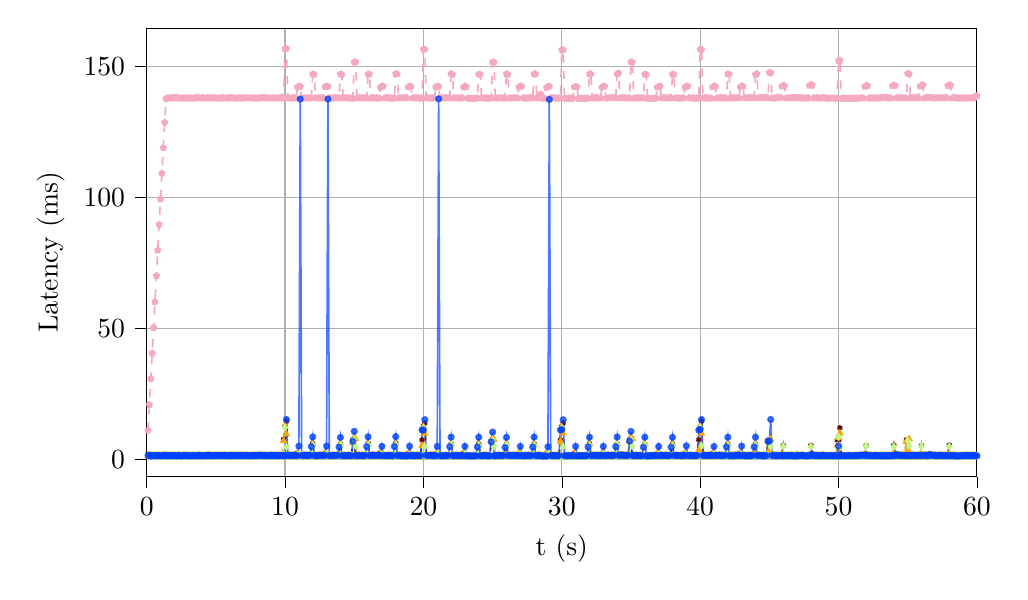
\begin{tikzpicture}

\definecolor{blue064255}{RGB}{0,64,255}
\definecolor{darkgrey176}{RGB}{176,176,176}
\definecolor{lightpink245169188}{RGB}{245,169,188}
\definecolor{maroon971111}{RGB}{97,11,11}
\definecolor{orange}{RGB}{255,165,0}
\definecolor{palegreen190247129}{RGB}{190,247,129}

\begin{axis}[
height=0.6\textwidth,
tick align=outside,
tick pos=left,
width=\textwidth,
x grid style={darkgrey176},
xlabel={t (s)},
xmajorgrids,
xmin=0, xmax=60,
xtick style={color=black},
y grid style={darkgrey176},
ylabel={Latency (ms)},
ymajorgrids,
ymin=-6.4958, ymax=164.6818,
ytick style={color=black}
]
\addplot [semithick, maroon971111, dash pattern=on 1pt off 3pt on 3pt off 3pt, mark=asterisk, mark size=1, mark options={solid}]
table {%
0.1 1.678
0.2 1.508
0.3 1.543
0.4 1.532
0.5 1.53
0.6 1.506
0.7 1.51
0.8 1.519
0.9 1.512
1 1.494
1.1 1.51
1.2 1.532
1.3 1.777
1.4 1.541
1.5 1.499
1.6 1.523
1.7 1.547
1.8 1.495
1.9 1.523
2 1.523
2.1 1.524
2.2 1.632
2.3 1.499
2.4 1.518
2.5 1.523
2.6 1.526
2.7 1.485
2.8 1.538
2.9 1.506
3 1.491
3.1 1.515
3.2 1.496
3.3 1.521
3.4 1.49
3.5 1.519
3.6 1.556
3.7 1.499
3.8 1.518
3.9 1.507
4 1.483
4.1 1.506
4.2 1.542
4.3 1.491
4.4 1.54
4.5 1.508
4.6 1.483
4.7 1.507
4.8 1.522
4.9 1.534
5 1.489
5.1 1.515
5.2 1.555
5.3 1.557
5.4 1.642
5.5 1.508
5.6 1.546
5.7 1.526
5.8 1.538
5.9 1.571
6 1.551
6.1 1.835
6.2 1.572
6.3 1.629
6.4 1.598
6.5 1.585
6.6 1.642
6.7 1.553
6.8 1.59
6.9 1.57
7 1.64
7.1 1.635
7.2 1.527
7.3 1.618
7.4 1.511
7.5 1.551
7.6 1.594
7.7 1.544
7.8 1.587
7.9 1.591
8 1.576
8.1 1.567
8.2 1.589
8.3 1.505
8.4 1.543
8.5 1.483
8.6 1.551
8.7 1.588
8.8 1.516
8.9 1.527
9 1.544
9.1 1.509
9.2 1.502
9.3 1.521
9.4 1.498
9.5 1.568
9.6 1.523
9.7 1.527
9.8 1.552
9.9 7.772
10 12.647
10.1 14.619
10.2 1.529
10.3 1.516
10.4 1.53
10.5 1.506
10.6 1.59
10.7 1.489
10.8 1.522
10.9 2.519
11 1.509
11.1 1.568
11.2 1.543
11.3 1.505
11.4 1.532
11.5 1.571
11.6 1.503
11.7 1.44
11.8 1.53
11.9 1.526
12 6.135
12.1 1.507
12.2 1.53
12.3 1.53
12.4 1.498
12.5 1.575
12.6 1.536
12.7 1.759
12.8 1.528
12.9 2.615
13 1.582
13.1 1.538
13.2 1.663
13.3 1.582
13.4 1.566
13.5 1.508
13.6 1.554
13.7 1.575
13.8 1.496
13.9 1.736
14 5.99
14.1 1.485
14.2 1.507
14.3 1.549
14.4 1.545
14.5 1.525
14.6 1.466
14.7 1.516
14.8 1.518
14.9 7.47
15 8.098
15.1 1.532
15.2 1.523
15.3 1.528
15.4 1.53
15.5 1.512
15.6 1.544
15.7 1.534
15.8 1.505
15.9 1.528
16 6.128
16.1 1.544
16.2 1.534
16.3 1.515
16.4 1.514
16.5 1.528
16.6 1.502
16.7 1.511
16.8 1.522
16.9 2.581
17 1.509
17.1 1.526
17.2 1.584
17.3 1.65
17.4 1.553
17.5 1.553
17.6 1.595
17.7 1.518
17.8 1.62
17.9 1.574
18 6.231
18.1 1.53
18.2 1.51
18.3 1.61
18.4 1.573
18.5 1.508
18.6 1.535
18.7 1.484
18.8 1.592
18.9 2.463
19 1.587
19.1 1.55
19.2 1.491
19.3 1.655
19.4 1.521
19.5 1.571
19.6 1.516
19.7 1.513
19.8 1.517
19.9 7.502
20 12.724
20.1 13.962
20.2 1.539
20.3 1.547
20.4 1.509
20.5 1.562
20.6 1.541
20.7 1.54
20.8 1.502
20.9 2.337
21 1.536
21.1 1.463
21.2 1.446
21.3 1.524
21.4 1.464
21.5 1.488
21.6 1.451
21.7 1.533
21.8 1.591
21.9 1.595
22 5.96
22.1 1.524
22.2 1.51
22.3 1.524
22.4 1.548
22.5 1.54
22.6 1.524
22.7 1.511
22.8 1.496
22.9 2.427
23 1.517
23.1 1.427
23.2 1.554
23.3 1.389
23.4 1.447
23.5 1.447
23.6 1.394
23.7 1.452
23.8 1.47
23.9 1.508
24 5.945
24.1 1.516
24.2 1.476
24.3 1.517
24.4 1.461
24.5 1.532
24.6 1.493
24.7 1.484
24.8 1.508
24.9 7.188
25 7.87
25.1 1.49
25.2 1.48
25.3 1.471
25.4 1.608
25.5 1.519
25.6 1.603
25.7 1.502
25.8 1.522
25.9 1.522
26 5.897
26.1 1.493
26.2 1.5
26.3 1.509
26.4 1.55
26.5 1.528
26.6 1.596
26.7 1.564
26.8 1.52
26.9 2.439
27 1.559
27.1 1.54
27.2 1.472
27.3 1.375
27.4 1.509
27.5 1.56
27.6 1.567
27.7 1.657
27.8 1.612
27.9 1.87
28 6.022
28.1 1.522
28.2 1.608
28.3 1.731
28.4 1.578
28.5 1.537
28.6 1.458
28.7 1.456
28.8 1.448
28.9 2.359
29 1.574
29.1 1.49
29.2 1.761
29.3 1.555
29.4 1.562
29.5 1.496
29.6 1.458
29.7 1.36
29.8 1.381
29.9 7.408
30 12.616
30.1 13.907
30.2 1.361
30.3 1.371
30.4 1.373
30.5 1.377
30.6 1.425
30.7 1.354
30.8 1.398
30.9 2.457
31 1.378
31.1 1.47
31.2 1.374
31.3 1.363
31.4 1.346
31.5 1.35
31.6 1.37
31.7 1.43
31.8 1.383
31.9 1.449
32 6.092
32.1 1.537
32.2 1.525
32.3 1.503
32.4 1.562
32.5 1.542
32.6 1.503
32.7 1.485
32.8 1.53
32.9 2.45
33 1.812
33.1 1.627
33.2 1.521
33.3 1.487
33.4 1.598
33.5 1.523
33.6 1.506
33.7 1.672
33.8 1.562
33.9 1.523
34 5.983
34.1 1.498
34.2 1.727
34.3 1.532
34.4 1.742
34.5 1.575
34.6 1.504
34.7 1.497
34.8 1.592
34.9 7.588
35 8.224
35.1 1.537
35.2 1.582
35.3 1.538
35.4 1.588
35.5 1.552
35.6 1.578
35.7 1.565
35.8 1.53
35.9 1.591
36 5.966
36.1 1.403
36.2 1.357
36.3 1.369
36.4 1.404
36.5 1.35
36.6 1.414
36.7 1.396
36.8 1.387
36.9 2.351
37 1.493
37.1 1.523
37.2 1.494
37.3 1.618
37.4 1.5
37.5 1.61
37.6 1.505
37.7 1.548
37.8 1.532
37.9 1.484
38 5.961
38.1 1.527
38.2 1.502
38.3 1.522
38.4 1.592
38.5 1.47
38.6 1.518
38.7 1.613
38.8 1.64
38.9 2.58
39 1.58
39.1 1.46
39.2 1.515
39.3 1.518
39.4 1.483
39.5 1.539
39.6 1.477
39.7 1.43
39.8 1.497
39.9 7.61
40 12.59
40.1 14.605
40.2 1.521
40.3 1.627
40.4 1.538
40.5 1.557
40.6 1.576
40.7 1.615
40.8 1.54
40.9 2.368
41 1.554
41.1 1.532
41.2 1.532
41.3 1.531
41.4 1.533
41.5 1.536
41.6 1.518
41.7 1.59
41.8 1.513
41.9 1.593
42 6.034
42.1 1.599
42.2 1.572
42.3 1.61
42.4 1.849
42.5 1.525
42.6 1.712
42.7 1.736
42.8 1.607
42.9 2.545
43 1.552
43.1 1.568
43.2 1.487
43.3 1.567
43.4 1.574
43.5 1.546
43.6 1.574
43.7 1.829
43.8 1.586
43.9 1.502
44 5.836
44.1 1.603
44.2 1.553
44.3 1.604
44.4 1.556
44.5 1.517
44.6 1.539
44.7 1.722
44.8 1.555
44.9 7.41
45 1.779
45.1 1.479
45.2 1.508
45.3 1.518
45.4 1.499
45.5 1.475
45.6 1.774
45.7 1.784
45.8 1.558
45.9 1.882
46 5.342
46.1 1.545
46.2 1.68
46.3 1.493
46.4 1.523
46.5 1.525
46.6 1.504
46.7 1.742
46.8 1.621
46.9 1.713
47 1.929
47.1 1.492
47.2 1.526
47.3 1.521
47.4 1.529
47.5 1.534
47.6 1.399
47.7 1.421
47.8 1.635
47.9 1.998
48 5.406
48.1 1.491
48.2 1.593
48.3 1.616
48.4 1.533
48.5 1.604
48.6 1.586
48.7 1.557
48.8 1.862
48.9 1.573
49 1.546
49.1 1.42
49.2 1.397
49.3 1.374
49.4 1.402
49.5 1.447
49.6 1.511
49.7 1.375
49.8 1.344
49.9 7.368
50 8.425
50.1 12.128
50.2 1.389
50.3 1.385
50.4 1.491
50.5 1.355
50.6 1.397
50.7 1.393
50.8 1.395
50.9 1.398
51 1.418
51.1 1.368
51.2 1.44
51.3 1.41
51.4 1.554
51.5 1.511
51.6 1.539
51.7 1.552
51.8 1.52
51.9 2.012
52 5.33
52.1 1.452
52.2 1.481
52.3 1.476
52.4 1.512
52.5 1.526
52.6 1.495
52.7 1.528
52.8 1.496
52.9 1.531
53 1.478
53.1 1.745
53.2 1.515
53.3 1.629
53.4 1.63
53.5 1.534
53.6 1.533
53.7 1.485
53.8 1.574
53.9 1.997
54 5.428
54.1 1.506
54.2 1.642
54.3 1.527
54.4 1.521
54.5 1.559
54.6 1.528
54.7 1.505
54.8 1.506
54.9 7.547
55 1.495
55.1 1.52
55.2 1.546
55.3 1.656
55.4 1.764
55.5 1.652
55.6 1.474
55.7 1.506
55.8 1.509
55.9 1.878
56 5.276
56.1 1.558
56.2 1.543
56.3 1.626
56.4 1.488
56.5 1.51
56.6 1.677
56.7 1.53
56.8 1.528
56.9 1.546
57 1.55
57.1 1.551
57.2 1.556
57.3 1.581
57.4 1.544
57.5 1.618
57.6 1.615
57.7 1.761
57.8 1.52
57.9 2.124
58 5.534
58.1 1.497
58.2 1.541
58.3 1.487
58.4 1.58
58.5 1.504
58.6 1.477
58.7 1.374
58.8 1.575
58.9 1.5
59 1.538
59.1 1.502
59.2 1.501
59.3 1.483
59.4 1.512
59.5 1.569
59.6 1.521
59.7 1.552
59.8 1.553
59.9 1.812
60 1.511
};
\addplot [semithick, lightpink245169188, dashed, mark=pentagon*, mark size=1, mark options={solid}]
table {%
0.1 11.123
0.2 20.939
0.3 30.868
0.4 40.597
0.5 50.345
0.6 60.211
0.7 70.179
0.8 79.912
0.9 89.75
1 99.454
1.1 109.263
1.2 118.993
1.3 128.741
1.4 137.771
1.5 138.019
1.6 138.081
1.7 137.994
1.8 137.944
1.9 138.242
2 138.032
2.1 138.077
2.2 138.295
2.3 137.966
2.4 137.974
2.5 137.94
2.6 137.94
2.7 138.016
2.8 138.036
2.9 137.949
3 137.978
3.1 138.031
3.2 138
3.3 137.931
3.4 137.965
3.5 137.972
3.6 138.281
3.7 138.073
3.8 138.126
3.9 137.923
4 138.099
4.1 138.09
4.2 138.014
4.3 137.954
4.4 138.197
4.5 138.042
4.6 138.026
4.7 137.999
4.8 138.073
4.9 138.041
5 137.956
5.1 137.989
5.2 137.969
5.3 138.022
5.4 137.964
5.5 138.254
5.6 138.014
5.7 137.973
5.8 138.003
5.9 137.968
6 138.162
6.1 138.208
6.2 137.989
6.3 137.972
6.4 137.931
6.5 137.95
6.6 138.007
6.7 138.066
6.8 138.041
6.9 137.944
7 138.002
7.1 138.112
7.2 137.974
7.3 137.978
7.4 138.081
7.5 137.977
7.6 137.974
7.7 137.983
7.8 137.968
7.9 138.004
8 137.958
8.1 137.974
8.2 138.139
8.3 138.01
8.4 138.079
8.5 138.246
8.6 138.003
8.7 137.983
8.8 138.005
8.9 138.065
9 137.991
9.1 138.028
9.2 138.095
9.3 137.973
9.4 137.969
9.5 138.044
9.6 138.03
9.7 138.037
9.8 138.455
9.9 138.051
10 156.761
10.1 156.901
10.2 138.002
10.3 137.979
10.4 137.951
10.5 137.926
10.6 138.145
10.7 137.988
10.8 137.972
10.9 142.174
11 142.543
11.1 142.456
11.2 137.923
11.3 138.025
11.4 138.019
11.5 138.058
11.6 137.943
11.7 137.999
11.8 138.056
11.9 137.995
12 147.092
12.1 147.054
12.2 138.084
12.3 138.004
12.4 137.987
12.5 138.044
12.6 137.967
12.7 138.233
12.8 138
12.9 142.326
13 142.584
13.1 142.447
13.2 138.078
13.3 138.081
13.4 137.936
13.5 138.035
13.6 138.17
13.7 137.999
13.8 138.066
13.9 138.046
14 147.15
14.1 147.01
14.2 138.238
14.3 138.01
14.4 138.028
14.5 138.145
14.6 138.032
14.7 137.959
14.8 137.938
14.9 137.935
15 151.698
15.1 151.775
15.2 137.973
15.3 138.072
15.4 138.045
15.5 137.981
15.6 138.05
15.7 138.099
15.8 138.053
15.9 137.989
16 147.13
16.1 147.097
16.2 137.958
16.3 138.129
16.4 138
16.5 137.977
16.6 138.063
16.7 137.937
16.8 137.97
16.9 142.11
17 142.595
17.1 142.491
17.2 138.023
17.3 138.121
17.4 138.067
17.5 138.032
17.6 137.969
17.7 137.959
17.8 137.963
17.9 137.977
18 147.285
18.1 147.233
18.2 138.013
18.3 138
18.4 138.009
18.5 138.081
18.6 138.014
18.7 138.028
18.8 138.083
18.9 142.177
19 142.53
19.1 142.428
19.2 137.932
19.3 138.1
19.4 138.061
19.5 138.024
19.6 138.063
19.7 137.949
19.8 137.95
19.9 137.989
20 156.619
20.1 156.602
20.2 137.986
20.3 138.071
20.4 137.998
20.5 137.908
20.6 137.999
20.7 138.055
20.8 137.987
20.9 142.182
21 142.482
21.1 142.452
21.2 138.029
21.3 137.989
21.4 138.083
21.5 137.94
21.6 138.122
21.7 138.014
21.8 138.117
21.9 138.041
22 147.294
22.1 147.038
22.2 138.02
22.3 138.01
22.4 138.004
22.5 138.014
22.6 137.998
22.7 137.947
22.8 138.165
22.9 142.113
23 142.582
23.1 142.317
23.2 137.906
23.3 137.838
23.4 137.933
23.5 137.808
23.6 137.827
23.7 137.825
23.8 137.96
23.9 137.997
24 147.053
24.1 147.027
24.2 137.984
24.3 137.997
24.4 137.95
24.5 138.036
24.6 138.043
24.7 137.959
24.8 137.937
24.9 138.071
25 151.693
25.1 151.654
25.2 137.971
25.3 137.957
25.4 138.038
25.5 138.073
25.6 138.019
25.7 138.017
25.8 137.969
25.9 137.935
26 147.235
26.1 147.027
26.2 137.984
26.3 138.009
26.4 138.014
26.5 137.979
26.6 138.012
26.7 138.049
26.8 138.056
26.9 142.183
27 142.518
27.1 142.518
27.2 138.02
27.3 137.877
27.4 137.995
27.5 137.964
27.6 138.013
27.7 138.037
27.8 138.078
27.9 138.185
28 147.21
28.1 147.172
28.2 138.032
28.3 138.026
28.4 139.35
28.5 139.464
28.6 137.958
28.7 137.849
28.8 137.822
28.9 141.982
29 142.366
29.1 142.536
29.2 138.037
29.3 138.067
29.4 137.981
29.5 138.044
29.6 137.927
29.7 137.887
29.8 137.954
29.9 137.878
30 156.459
30.1 156.396
30.2 137.941
30.3 137.854
30.4 137.845
30.5 137.871
30.6 137.954
30.7 137.904
30.8 137.873
30.9 142.186
31 142.318
31.1 142.315
31.2 137.871
31.3 137.922
31.4 137.84
31.5 137.856
31.6 137.803
31.7 137.868
31.8 137.914
31.9 137.929
32 147.21
32.1 147.163
32.2 137.982
32.3 137.943
32.4 138.117
32.5 138.26
32.6 137.959
32.7 137.982
32.8 138.019
32.9 142.155
33 142.418
33.1 142.472
33.2 137.98
33.3 137.97
33.4 138.02
33.5 138.087
33.6 138.097
33.7 138.227
33.8 137.971
33.9 137.995
34 147.242
34.1 147.527
34.2 138.002
34.3 138.136
34.4 138.084
34.5 138.162
34.6 138.062
34.7 137.973
34.8 137.982
34.9 138.056
35 151.784
35.1 151.68
35.2 137.951
35.3 138.006
35.4 137.998
35.5 138.099
35.6 138.006
35.7 138.033
35.8 137.995
35.9 138.051
36 147.108
36.1 146.988
36.2 137.808
36.3 137.894
36.4 137.878
36.5 137.896
36.6 137.867
36.7 137.863
36.8 137.938
36.9 142.123
37 142.372
37.1 142.478
37.2 137.98
37.3 138.063
37.4 138.07
37.5 138.028
37.6 138.053
37.7 137.959
37.8 138.126
37.9 138.067
38 147.14
38.1 147.01
38.2 137.999
38.3 138.055
38.4 137.963
38.5 137.946
38.6 137.915
38.7 137.994
38.8 138.002
38.9 142.131
39 142.518
39.1 142.523
39.2 137.989
39.3 138.003
39.4 137.976
39.5 137.952
39.6 137.862
39.7 137.948
39.8 138
39.9 137.951
40 156.593
40.1 156.541
40.2 138.016
40.3 137.969
40.4 138.196
40.5 137.986
40.6 137.967
40.7 137.954
40.8 137.949
40.9 142.179
41 142.574
41.1 142.423
41.2 137.979
41.3 138.045
41.4 137.984
41.5 138.208
41.6 138.009
41.7 138.045
41.8 138.054
41.9 137.945
42 147.153
42.1 147.073
42.2 138.135
42.3 137.968
42.4 138.201
42.5 138.016
42.6 137.972
42.7 138.118
42.8 138.051
42.9 142.213
43 142.578
43.1 142.508
43.2 137.977
43.3 137.977
43.4 138.174
43.5 138.083
43.6 138.153
43.7 138.183
43.8 138.039
43.9 138.16
44 147.029
44.1 147.289
44.2 138.033
44.3 137.996
44.4 138.168
44.5 138.051
44.6 138.073
44.7 138.349
44.8 138.219
44.9 138.003
45 147.721
45.1 147.687
45.2 138.052
45.3 137.969
45.4 138.056
45.5 138.035
45.6 138.292
45.7 138.011
45.8 138.261
45.9 142.466
46 142.793
46.1 142.624
46.2 137.978
46.3 138.024
46.4 138.002
46.5 138.042
46.6 138.186
46.7 138.105
46.8 138.058
46.9 138.068
47 138.233
47.1 137.99
47.2 138.277
47.3 137.965
47.4 138.036
47.5 137.98
47.6 137.905
47.7 137.889
47.8 138.118
47.9 142.797
48 143.052
48.1 143
48.2 138.066
48.3 138.039
48.4 138.071
48.5 138.042
48.6 137.96
48.7 137.992
48.8 138.161
48.9 138.088
49 138.147
49.1 137.955
49.2 137.91
49.3 137.885
49.4 137.946
49.5 137.976
49.6 137.98
49.7 137.958
49.8 137.863
49.9 137.936
50 152.264
50.1 152.376
50.2 137.896
50.3 137.875
50.4 137.963
50.5 137.842
50.6 137.796
50.7 137.883
50.8 137.871
50.9 137.869
51 137.924
51.1 137.868
51.2 137.965
51.3 137.886
51.4 137.85
51.5 137.994
51.6 137.987
51.7 138.046
51.8 137.982
51.9 142.403
52 142.791
52.1 142.739
52.2 137.975
52.3 137.949
52.4 137.935
52.5 138.015
52.6 138.005
52.7 138.021
52.8 137.958
52.9 137.974
53 137.96
53.1 138.17
53.2 138.101
53.3 138.25
53.4 138.095
53.5 138.157
53.6 138.099
53.7 137.968
53.8 137.972
53.9 142.665
54 142.858
54.1 142.761
54.2 138.144
54.3 138.001
54.4 138.103
54.5 138.165
54.6 138.048
54.7 137.987
54.8 138.003
54.9 138.033
55 147.364
55.1 147.29
55.2 138.014
55.3 138.018
55.4 138.09
55.5 138.073
55.6 138.039
55.7 138.219
55.8 137.975
55.9 142.508
56 142.88
56.1 143.023
56.2 137.939
56.3 138.067
56.4 138.243
56.5 138.227
56.6 138.109
56.7 138.141
56.8 138.058
56.9 138.064
57 138.036
57.1 138.014
57.2 138.109
57.3 138.026
57.4 137.983
57.5 138.101
57.6 138.042
57.7 138.091
57.8 138.139
57.9 142.707
58 142.909
58.1 142.931
58.2 137.947
58.3 138.213
58.4 138.167
58.5 138.129
58.6 137.886
58.7 137.88
58.8 137.98
58.9 138.072
59 138.044
59.1 137.952
59.2 137.961
59.3 138.001
59.4 138.004
59.5 138.049
59.6 138.058
59.7 138.073
59.8 138.028
59.9 138.744
60 138.845
};
\addplot [semithick, orange, dashed, mark=triangle*, mark size=1, mark options={solid}]
table {%
0.1 1.477
0.2 1.563
0.3 1.483
0.4 1.487
0.5 1.486
0.6 1.497
0.7 1.518
0.8 1.514
0.9 1.512
1 1.431
1.1 1.514
1.2 1.488
1.3 1.57
1.4 1.463
1.5 1.482
1.6 1.5
1.7 1.496
1.8 1.475
1.9 1.5
2 1.471
2.1 1.506
2.2 1.518
2.3 1.524
2.4 1.478
2.5 1.466
2.6 1.469
2.7 1.456
2.8 1.457
2.9 1.489
3 1.505
3.1 1.498
3.2 1.499
3.3 1.502
3.4 1.515
3.5 1.497
3.6 1.521
3.7 1.431
3.8 1.502
3.9 1.435
4 1.424
4.1 1.446
4.2 1.466
4.3 1.529
4.4 1.513
4.5 1.487
4.6 1.522
4.7 1.446
4.8 1.506
4.9 1.484
5 1.336
5.1 1.465
5.2 1.539
5.3 1.481
5.4 1.494
5.5 1.519
5.6 1.496
5.7 1.489
5.8 1.467
5.9 1.511
6 1.477
6.1 1.477
6.2 1.513
6.3 1.516
6.4 1.495
6.5 1.506
6.6 1.52
6.7 1.517
6.8 1.503
6.9 1.532
7 1.482
7.1 1.499
7.2 1.5
7.3 1.568
7.4 1.46
7.5 1.529
7.6 1.387
7.7 1.512
7.8 1.495
7.9 1.644
8 1.483
8.1 1.504
8.2 1.487
8.3 1.511
8.4 1.536
8.5 1.555
8.6 1.456
8.7 1.49
8.8 1.481
8.9 1.464
9 1.519
9.1 1.504
9.2 1.506
9.3 1.49
9.4 1.468
9.5 1.501
9.6 1.461
9.7 1.472
9.8 1.499
9.9 7.178
10 12.802
10.1 9.653
10.2 1.483
10.3 1.5
10.4 1.457
10.5 1.478
10.6 1.492
10.7 1.516
10.8 1.483
10.9 2.419
11 1.389
11.1 1.466
11.2 1.56
11.3 1.513
11.4 1.481
11.5 1.492
11.6 1.514
11.7 1.474
11.8 1.487
11.9 1.485
12 5.963
12.1 1.522
12.2 1.417
12.3 1.494
12.4 1.519
12.5 1.496
12.6 1.52
12.7 1.499
12.8 1.495
12.9 2.424
13 1.487
13.1 1.5
13.2 1.502
13.3 1.488
13.4 1.492
13.5 1.495
13.6 1.506
13.7 1.494
13.8 1.47
13.9 1.571
14 6.141
14.1 1.505
14.2 1.474
14.3 1.489
14.4 1.506
14.5 1.535
14.6 1.501
14.7 1.472
14.8 1.533
14.9 6.336
15 8.168
15.1 7.992
15.2 1.494
15.3 1.494
15.4 1.497
15.5 1.455
15.6 1.505
15.7 1.473
15.8 1.488
15.9 1.522
16 5.96
16.1 1.486
16.2 1.516
16.3 1.48
16.4 1.493
16.5 1.579
16.6 1.472
16.7 1.505
16.8 1.512
16.9 2.365
17 1.418
17.1 1.487
17.2 1.493
17.3 1.488
17.4 1.494
17.5 1.501
17.6 1.461
17.7 1.472
17.8 1.461
17.9 1.511
18 6.042
18.1 1.444
18.2 1.469
18.3 1.52
18.4 1.465
18.5 1.454
18.6 1.465
18.7 1.424
18.8 1.517
18.9 2.305
19 1.52
19.1 1.5
19.2 1.477
19.3 1.554
19.4 1.499
19.5 1.617
19.6 1.472
19.7 1.441
19.8 1.479
19.9 5.304
20 12.564
20.1 9.978
20.2 1.498
20.3 1.51
20.4 1.509
20.5 1.493
20.6 1.474
20.7 1.496
20.8 1.478
20.9 2.434
21 1.443
21.1 1.634
21.2 1.437
21.3 1.46
21.4 1.462
21.5 1.447
21.6 1.474
21.7 1.432
21.8 1.478
21.9 1.514
22 6.041
22.1 1.469
22.2 1.467
22.3 1.497
22.4 1.501
22.5 1.522
22.6 1.476
22.7 1.53
22.8 1.488
22.9 2.578
23 1.47
23.1 1.358
23.2 1.405
23.3 1.345
23.4 1.406
23.5 1.33
23.6 1.474
23.7 1.358
23.8 1.471
23.9 1.551
24 5.859
24.1 1.462
24.2 1.464
24.3 1.5
24.4 1.467
24.5 1.49
24.6 1.493
24.7 1.442
24.8 1.479
24.9 7.02
25 7.956
25.1 7.586
25.2 1.507
25.3 1.459
25.4 1.514
25.5 1.473
25.6 1.483
25.7 1.47
25.8 1.596
25.9 1.473
26 5.926
26.1 1.466
26.2 1.54
26.3 1.475
26.4 1.463
26.5 1.481
26.6 1.491
26.7 1.459
26.8 1.509
26.9 2.518
27 1.553
27.1 1.539
27.2 1.518
27.3 1.356
27.4 1.462
27.5 1.508
27.6 1.483
27.7 1.525
27.8 1.484
27.9 1.643
28 5.921
28.1 1.509
28.2 1.459
28.3 1.748
28.4 1.509
28.5 1.505
28.6 1.362
28.7 1.343
28.8 1.349
28.9 2.45
29 1.492
29.1 1.469
29.2 1.567
29.3 1.465
29.4 1.478
29.5 1.534
29.6 1.512
29.7 1.329
29.8 1.333
29.9 6.866
30 12.453
30.1 10.051
30.2 1.374
30.3 1.329
30.4 1.308
30.5 1.382
30.6 1.325
30.7 1.372
30.8 1.369
30.9 2.309
31 1.379
31.1 1.334
31.2 1.343
31.3 1.319
31.4 1.323
31.5 1.318
31.6 1.325
31.7 1.338
31.8 1.351
31.9 1.334
32 5.986
32.1 1.433
32.2 1.522
32.3 1.522
32.4 1.508
32.5 1.491
32.6 1.503
32.7 1.408
32.8 1.452
32.9 2.534
33 1.643
33.1 1.497
33.2 1.461
33.3 1.478
33.4 1.529
33.5 1.506
33.6 1.48
33.7 1.454
33.8 1.493
33.9 1.493
34 6.055
34.1 1.597
34.2 1.55
34.3 1.483
34.4 1.798
34.5 1.523
34.6 1.487
34.7 1.507
34.8 1.461
34.9 7.15
35 8.074
35.1 7.934
35.2 1.512
35.3 1.471
35.4 1.473
35.5 1.53
35.6 1.453
35.7 1.48
35.8 1.479
35.9 1.473
36 6.035
36.1 1.373
36.2 1.372
36.3 1.34
36.4 1.32
36.5 1.373
36.6 1.349
36.7 1.391
36.8 1.377
36.9 2.438
37 1.612
37.1 1.509
37.2 1.459
37.3 1.484
37.4 1.486
37.5 1.489
37.6 1.516
37.7 1.468
37.8 1.444
37.9 1.443
38 5.874
38.1 1.493
38.2 1.459
38.3 1.448
38.4 1.427
38.5 1.377
38.6 1.432
38.7 1.451
38.8 1.495
38.9 2.424
39 1.476
39.1 1.471
39.2 1.479
39.3 1.487
39.4 1.474
39.5 1.489
39.6 1.345
39.7 1.352
39.8 1.472
39.9 3.559
40 12.737
40.1 9.995
40.2 1.516
40.3 1.541
40.4 1.471
40.5 1.514
40.6 1.533
40.7 1.467
40.8 1.487
40.9 2.528
41 1.535
41.1 1.497
41.2 1.487
41.3 1.5
41.4 1.487
41.5 1.479
41.6 1.462
41.7 1.516
41.8 1.475
41.9 1.481
42 5.944
42.1 1.54
42.2 1.478
42.3 1.45
42.4 1.61
42.5 1.487
42.6 1.495
42.7 1.721
42.8 1.53
42.9 2.405
43 1.481
43.1 1.498
43.2 1.514
43.3 1.576
43.4 1.49
43.5 1.462
43.6 1.474
43.7 1.561
43.8 1.732
43.9 1.509
44 5.916
44.1 1.604
44.2 1.45
44.3 1.486
44.4 1.458
44.5 1.46
44.6 1.721
44.7 1.424
44.8 1.528
44.9 7.246
45 3.521
45.1 7.718
45.2 1.46
45.3 1.492
45.4 1.535
45.5 1.474
45.6 1.573
45.7 1.516
45.8 1.642
45.9 1.954
46 1.416
46.1 1.457
46.2 1.482
46.3 1.543
46.4 1.499
46.5 1.487
46.6 1.523
46.7 1.497
46.8 1.479
46.9 1.799
47 1.701
47.1 1.409
47.2 1.472
47.3 1.515
47.4 1.521
47.5 1.441
47.6 1.344
47.7 1.345
47.8 1.502
47.9 1.842
48 1.493
48.1 1.483
48.2 1.507
48.3 1.51
48.4 1.491
48.5 1.509
48.6 1.467
48.7 1.478
48.8 1.633
48.9 1.632
49 1.402
49.1 1.326
49.2 1.337
49.3 1.362
49.4 1.346
49.5 1.361
49.6 1.386
49.7 1.338
49.8 1.386
49.9 5.45
50 8.359
50.1 10.063
50.2 1.322
50.3 1.339
50.4 1.459
50.5 1.285
50.6 1.331
50.7 1.432
50.8 1.329
50.9 1.306
51 1.38
51.1 1.325
51.2 1.515
51.3 1.466
51.4 1.356
51.5 1.449
51.6 1.527
51.7 1.472
51.8 1.535
51.9 1.837
52 1.531
52.1 1.494
52.2 1.491
52.3 1.506
52.4 1.464
52.5 1.398
52.6 1.475
52.7 1.506
52.8 1.47
52.9 1.457
53 1.453
53.1 1.592
53.2 1.668
53.3 1.522
53.4 1.599
53.5 1.624
53.6 1.473
53.7 1.468
53.8 1.486
53.9 1.831
54 1.419
54.1 1.499
54.2 1.711
54.3 1.483
54.4 1.486
54.5 1.641
54.6 1.482
54.7 1.441
54.8 1.464
54.9 6.949
55 3.689
55.1 7.857
55.2 1.469
55.3 1.655
55.4 1.551
55.5 1.453
55.6 1.525
55.7 1.481
55.8 1.515
55.9 2.049
56 1.505
56.1 1.649
56.2 1.488
56.3 1.485
56.4 1.49
56.5 1.514
56.6 1.802
56.7 1.459
56.8 1.487
56.9 1.486
57 1.514
57.1 1.483
57.2 1.472
57.3 1.497
57.4 1.502
57.5 1.519
57.6 1.511
57.7 1.627
57.8 1.508
57.9 1.963
58 1.543
58.1 1.463
58.2 1.472
58.3 1.477
58.4 1.646
58.5 1.39
58.6 1.421
58.7 1.47
58.8 1.506
58.9 1.497
59 1.514
59.1 1.483
59.2 1.5
59.3 1.477
59.4 1.523
59.5 1.451
59.6 1.5
59.7 1.682
59.8 1.492
59.9 1.446
60 1.458
};
\addplot [semithick, palegreen190247129, dash pattern=on 1pt off 3pt on 3pt off 3pt, mark=diamond*, mark size=1, mark options={solid}]
table {%
0.1 1.402
0.2 1.498
0.3 1.51
0.4 1.406
0.5 1.442
0.6 1.452
0.7 1.542
0.8 1.402
0.9 1.457
1 1.419
1.1 1.561
1.2 1.469
1.3 1.441
1.4 1.541
1.5 1.45
1.6 1.416
1.7 1.467
1.8 1.443
1.9 1.626
2 1.436
2.1 1.488
2.2 1.624
2.3 1.455
2.4 1.391
2.5 1.392
2.6 1.399
2.7 1.451
2.8 1.405
2.9 1.437
3 1.42
3.1 1.424
3.2 1.449
3.3 1.533
3.4 1.522
3.5 1.455
3.6 1.787
3.7 1.43
3.8 1.521
3.9 1.509
4 1.459
4.1 1.386
4.2 1.524
4.3 1.652
4.4 1.461
4.5 1.59
4.6 1.469
4.7 1.451
4.8 1.455
4.9 1.524
5 1.313
5.1 1.463
5.2 1.425
5.3 1.445
5.4 1.443
5.5 1.424
5.6 1.455
5.7 1.46
5.8 1.444
5.9 1.446
6 1.571
6.1 1.534
6.2 1.465
6.3 1.444
6.4 1.448
6.5 1.465
6.6 1.436
6.7 1.464
6.8 1.484
6.9 1.452
7 1.514
7.1 1.458
7.2 1.417
7.3 1.448
7.4 1.444
7.5 1.453
7.6 1.447
7.7 1.441
7.8 1.453
7.9 1.436
8 1.514
8.1 1.399
8.2 1.459
8.3 1.429
8.4 1.437
8.5 1.588
8.6 1.423
8.7 1.432
8.8 1.441
8.9 1.428
9 1.421
9.1 1.452
9.2 1.434
9.3 1.447
9.4 1.542
9.5 1.413
9.6 1.442
9.7 1.516
9.8 1.443
9.9 2.096
10 12.285
10.1 4.783
10.2 1.421
10.3 1.446
10.4 1.48
10.5 1.458
10.6 1.447
10.7 1.438
10.8 1.531
10.9 1.553
11 1.914
11.1 1.441
11.2 1.456
11.3 1.451
11.4 1.449
11.5 1.447
11.6 1.424
11.7 1.453
11.8 1.453
11.9 1.445
12 5.539
12.1 1.55
12.2 1.467
12.3 1.432
12.4 1.468
12.5 1.461
12.6 1.449
12.7 1.542
12.8 1.442
12.9 1.489
13 2.01
13.1 1.459
13.2 1.445
13.3 1.452
13.4 1.464
13.5 1.452
13.6 1.44
13.7 1.455
13.8 1.449
13.9 1.452
14 5.598
14.1 1.463
14.2 1.467
14.3 1.433
14.4 1.527
14.5 1.487
14.6 1.513
14.7 1.429
14.8 1.538
14.9 1.53
15 7.774
15.1 5.157
15.2 1.519
15.3 1.415
15.4 1.462
15.5 1.445
15.6 1.46
15.7 1.487
15.8 1.544
15.9 1.441
16 5.528
16.1 1.49
16.2 1.448
16.3 1.443
16.4 1.411
16.5 1.442
16.6 1.448
16.7 1.416
16.8 1.447
16.9 1.433
17 1.969
17.1 1.434
17.2 1.438
17.3 1.436
17.4 1.454
17.5 1.61
17.6 1.46
17.7 1.617
17.8 1.43
17.9 1.642
18 5.631
18.1 1.413
18.2 1.436
18.3 1.451
18.4 1.515
18.5 1.441
18.6 1.451
18.7 1.491
18.8 1.419
18.9 1.447
19 1.855
19.1 1.576
19.2 1.531
19.3 1.43
19.4 1.575
19.5 1.503
19.6 1.464
19.7 1.567
19.8 1.43
19.9 1.464
20 12.124
20.1 4.945
20.2 1.5
20.3 1.469
20.4 1.454
20.5 1.453
20.6 1.462
20.7 1.521
20.8 1.433
20.9 1.483
21 1.962
21.1 1.434
21.2 1.536
21.3 1.429
21.4 1.546
21.5 1.455
21.6 1.54
21.7 1.526
21.8 1.449
21.9 1.504
22 5.607
22.1 1.431
22.2 1.437
22.3 1.464
22.4 1.497
22.5 1.532
22.6 1.516
22.7 1.455
22.8 1.43
22.9 1.468
23 2.075
23.1 1.3
23.2 1.316
23.3 1.319
23.4 1.294
23.5 1.306
23.6 1.32
23.7 1.328
23.8 1.452
23.9 1.434
24 5.35
24.1 1.439
24.2 1.493
24.3 1.44
24.4 1.449
24.5 1.431
24.6 1.525
24.7 1.422
24.8 1.553
24.9 1.43
25 7.505
25.1 4.972
25.2 1.473
25.3 1.458
25.4 1.45
25.5 1.433
25.6 1.476
25.7 1.511
25.8 1.436
25.9 1.46
26 5.659
26.1 1.403
26.2 1.426
26.3 1.442
26.4 1.417
26.5 1.518
26.6 1.446
26.7 1.518
26.8 1.415
26.9 1.45
27 2.063
27.1 1.523
27.2 1.408
27.3 1.369
27.4 1.534
27.5 1.495
27.6 1.47
27.7 1.452
27.8 1.477
27.9 1.505
28 5.425
28.1 1.462
28.2 1.446
28.3 1.464
28.4 1.418
28.5 1.423
28.6 1.32
28.7 1.34
28.8 1.319
28.9 1.322
29 1.975
29.1 1.453
29.2 1.475
29.3 1.528
29.4 1.524
29.5 1.476
29.6 1.424
29.7 1.343
29.8 1.333
29.9 1.323
30 12.016
30.1 4.857
30.2 1.329
30.3 1.359
30.4 1.316
30.5 1.333
30.6 1.321
30.7 1.313
30.8 1.323
30.9 1.324
31 1.851
31.1 1.312
31.2 1.322
31.3 1.417
31.4 1.408
31.5 1.326
31.6 1.417
31.7 1.345
31.8 1.323
31.9 1.326
32 5.498
32.1 1.437
32.2 1.446
32.3 1.447
32.4 1.423
32.5 1.448
32.6 1.447
32.7 1.528
32.8 1.504
32.9 1.41
33 2.09
33.1 1.526
33.2 1.505
33.3 1.453
33.4 1.428
33.5 1.438
33.6 1.456
33.7 1.621
33.8 1.451
33.9 1.46
34 5.801
34.1 1.666
34.2 1.524
34.3 1.487
34.4 1.598
34.5 1.517
34.6 1.438
34.7 1.46
34.8 1.435
34.9 1.461
35 7.614
35.1 5.137
35.2 1.51
35.3 1.426
35.4 1.593
35.5 1.431
35.6 1.462
35.7 1.547
35.8 1.471
35.9 1.516
36 5.669
36.1 1.32
36.2 1.324
36.3 1.334
36.4 1.312
36.5 1.334
36.6 1.329
36.7 1.363
36.8 1.325
36.9 1.321
37 2.006
37.1 1.489
37.2 1.464
37.3 1.434
37.4 1.444
37.5 1.431
37.6 1.43
37.7 1.465
37.8 1.433
37.9 1.432
38 5.36
38.1 1.422
38.2 1.449
38.3 1.508
38.4 1.435
38.5 1.427
38.6 1.491
38.7 1.509
38.8 1.427
38.9 1.45
39 1.954
39.1 1.44
39.2 1.443
39.3 1.472
39.4 1.53
39.5 1.432
39.6 1.368
39.7 1.349
39.8 1.429
39.9 1.412
40 12.233
40.1 5.217
40.2 1.537
40.3 1.458
40.4 1.437
40.5 1.559
40.6 1.443
40.7 1.458
40.8 1.471
40.9 1.477
41 2.082
41.1 1.434
41.2 1.522
41.3 1.404
41.4 1.449
41.5 1.692
41.6 1.498
41.7 1.45
41.8 1.477
41.9 1.427
42 5.431
42.1 1.513
42.2 1.518
42.3 1.427
42.4 1.442
42.5 1.418
42.6 1.45
42.7 1.44
42.8 1.45
42.9 1.507
43 1.941
43.1 1.428
43.2 1.487
43.3 1.434
43.4 1.754
43.5 1.54
43.6 1.596
43.7 1.537
43.8 1.433
43.9 1.57
44 5.55
44.1 1.447
44.2 1.482
44.3 1.445
44.4 1.511
44.5 1.506
44.6 1.668
44.7 1.52
44.8 1.7
44.9 1.45
45 7.275
45.1 4.96
45.2 1.435
45.3 1.438
45.4 1.71
45.5 1.584
45.6 1.454
45.7 1.48
45.8 1.499
45.9 1.497
46 5.034
46.1 1.439
46.2 1.434
46.3 1.522
46.4 1.47
46.5 1.517
46.6 1.453
46.7 1.657
46.8 1.431
46.9 1.702
47 1.493
47.1 1.426
47.2 1.439
47.3 1.426
47.4 1.47
47.5 1.427
47.6 1.33
47.7 1.32
47.8 1.693
47.9 1.516
48 4.915
48.1 1.48
48.2 1.587
48.3 1.446
48.4 1.442
48.5 1.512
48.6 1.444
48.7 1.454
48.8 1.745
48.9 1.44
49 1.481
49.1 1.34
49.2 1.314
49.3 1.319
49.4 1.369
49.5 1.418
49.6 1.486
49.7 1.323
49.8 1.346
49.9 1.315
50 8.627
50.1 4.863
50.2 1.305
50.3 1.325
50.4 1.316
50.5 1.322
50.6 1.322
50.7 1.316
50.8 1.319
50.9 1.318
51 1.316
51.1 1.368
51.2 1.325
51.3 1.329
51.4 1.38
51.5 1.52
51.6 1.462
51.7 1.452
51.8 1.506
51.9 1.442
52 5.163
52.1 1.567
52.2 1.495
52.3 1.493
52.4 1.456
52.5 1.423
52.6 1.415
52.7 1.449
52.8 1.409
52.9 1.428
53 1.509
53.1 1.537
53.2 1.586
53.3 1.444
53.4 1.621
53.5 1.623
53.6 1.536
53.7 1.498
53.8 1.428
53.9 1.421
54 4.906
54.1 1.442
54.2 1.424
54.3 1.428
54.4 1.56
54.5 1.433
54.6 1.448
54.7 1.448
54.8 1.532
54.9 1.438
55 7.176
55.1 5.054
55.2 1.532
55.3 1.535
55.4 1.416
55.5 1.529
55.6 1.575
55.7 1.581
55.8 1.431
55.9 1.446
56 5.034
56.1 1.456
56.2 1.507
56.3 1.578
56.4 1.904
56.5 1.719
56.6 1.43
56.7 1.43
56.8 1.436
56.9 1.529
57 1.449
57.1 1.473
57.2 1.432
57.3 1.572
57.4 1.516
57.5 1.546
57.6 1.549
57.7 1.52
57.8 1.528
57.9 1.459
58 5.032
58.1 1.458
58.2 1.426
58.3 1.671
58.4 1.411
58.5 1.646
58.6 1.408
58.7 1.357
58.8 1.498
58.9 1.436
59 1.513
59.1 1.468
59.2 1.499
59.3 1.491
59.4 1.449
59.5 1.513
59.6 1.664
59.7 1.51
59.8 1.433
59.9 1.514
60 1.482
};
\addplot [semithick, blue064255, opacity=0.7, mark=*, mark size=1, mark options={solid}]
table {%
0.1 1.607
0.2 1.672
0.3 1.389
0.4 1.44
0.5 1.572
0.6 1.421
0.7 1.546
0.8 1.499
0.9 1.435
1 1.452
1.1 1.431
1.2 1.577
1.3 1.557
1.4 1.59
1.5 1.417
1.6 1.466
1.7 1.562
1.8 1.489
1.9 1.56
2 1.463
2.1 1.469
2.2 1.441
2.3 1.518
2.4 1.455
2.5 1.363
2.6 1.502
2.7 1.628
2.8 1.508
2.9 1.457
3 1.433
3.1 1.442
3.2 1.489
3.3 1.452
3.4 1.464
3.5 1.55
3.6 1.499
3.7 1.44
3.8 1.678
3.9 1.436
4 1.477
4.1 1.492
4.2 1.454
4.3 1.593
4.4 1.513
4.5 1.67
4.6 1.558
4.7 1.416
4.8 1.502
4.9 1.611
5 1.438
5.1 1.567
5.2 1.532
5.3 1.544
5.4 1.559
5.5 1.501
5.6 1.62
5.7 1.591
5.8 1.428
5.9 1.53
6 1.562
6.1 1.451
6.2 1.552
6.3 1.486
6.4 1.579
6.5 1.442
6.6 1.542
6.7 1.525
6.8 1.526
6.9 1.547
7 1.524
7.1 1.474
7.2 1.542
7.3 1.571
7.4 1.47
7.5 1.471
7.6 1.543
7.7 1.51
7.8 1.504
7.9 1.6
8 1.468
8.1 1.657
8.2 1.639
8.3 1.583
8.4 1.517
8.5 1.568
8.6 1.466
8.7 1.591
8.8 1.456
8.9 1.494
9 1.663
9.1 1.522
9.2 1.557
9.3 1.497
9.4 1.651
9.5 1.438
9.6 1.512
9.7 1.589
9.8 1.527
9.9 1.5
10 1.528
10.1 15.301
10.2 1.56
10.3 1.635
10.4 1.571
10.5 1.518
10.6 1.55
10.7 1.652
10.8 1.575
10.9 1.527
11 5.132
11.1 137.656
11.2 1.528
11.3 1.609
11.4 1.619
11.5 1.581
11.6 1.572
11.7 1.597
11.8 1.588
11.9 4.963
12 8.641
12.1 1.561
12.2 1.492
12.3 1.467
12.4 1.548
12.5 1.608
12.6 1.593
12.7 1.573
12.8 1.612
12.9 1.574
13 5.092
13.1 137.625
13.2 1.49
13.3 1.507
13.4 1.54
13.5 1.561
13.6 1.566
13.7 1.607
13.8 1.565
13.9 4.773
14 8.441
14.1 1.472
14.2 1.519
14.3 1.446
14.4 1.466
14.5 1.532
14.6 1.566
14.7 1.514
14.8 1.415
14.9 6.935
15 10.76
15.1 1.53
15.2 1.475
15.3 1.58
15.4 1.579
15.5 1.509
15.6 1.487
15.7 1.486
15.8 1.552
15.9 4.928
16 8.676
16.1 1.574
16.2 1.608
16.3 1.654
16.4 1.635
16.5 1.578
16.6 1.601
16.7 1.627
16.8 1.602
16.9 1.562
17 5.035
17.1 1.489
17.2 1.47
17.3 1.507
17.4 1.434
17.5 1.562
17.6 1.529
17.7 1.545
17.8 1.462
17.9 5.007
18 8.767
18.1 1.58
18.2 1.519
18.3 1.61
18.4 1.46
18.5 1.435
18.6 1.524
18.7 1.345
18.8 1.436
18.9 1.528
19 5.105
19.1 1.552
19.2 1.528
19.3 1.495
19.4 1.482
19.5 1.517
19.6 1.546
19.7 1.555
19.8 1.504
19.9 11.3
20 11.218
20.1 15.213
20.2 1.608
20.3 1.536
20.4 1.591
20.5 1.59
20.6 1.613
20.7 1.561
20.8 1.481
20.9 1.483
21 5.005
21.1 137.72
21.2 1.485
21.3 1.473
21.4 1.408
21.5 1.524
21.6 1.488
21.7 1.551
21.8 1.521
21.9 4.93
22 8.565
22.1 1.595
22.2 1.45
22.3 1.504
22.4 1.615
22.5 1.481
22.6 1.485
22.7 1.478
22.8 1.618
22.9 1.43
23 5.05
23.1 1.427
23.2 1.411
23.3 1.496
23.4 1.328
23.5 1.412
23.6 1.356
23.7 1.412
23.8 1.423
23.9 4.831
24 8.527
24.1 1.464
24.2 1.499
24.3 1.438
24.4 1.608
24.5 1.58
24.6 1.403
24.7 1.438
24.8 1.424
24.9 6.743
25 10.487
25.1 1.417
25.2 1.471
25.3 1.464
25.4 1.619
25.5 1.529
25.6 1.524
25.7 1.524
25.8 1.565
25.9 4.611
26 8.448
26.1 1.526
26.2 1.508
26.3 1.583
26.4 1.528
26.5 1.637
26.6 1.544
26.7 1.579
26.8 1.493
26.9 1.488
27 5.016
27.1 1.606
27.2 1.506
27.3 1.389
27.4 1.617
27.5 1.522
27.6 1.496
27.7 1.502
27.8 1.543
27.9 4.808
28 8.586
28.1 1.534
28.2 1.485
28.3 1.489
28.4 1.63
28.5 1.398
28.6 1.367
28.7 1.344
28.8 1.38
28.9 1.328
29 4.854
29.1 137.513
29.2 1.562
29.3 1.55
29.4 1.546
29.5 1.508
29.6 1.534
29.7 1.408
29.8 1.52
29.9 11.286
30 11.413
30.1 15.195
30.2 1.477
30.3 1.449
30.4 1.444
30.5 1.481
30.6 1.479
30.7 1.442
30.8 1.482
30.9 1.48
31 5.03
31.1 1.451
31.2 1.415
31.3 1.482
31.4 1.448
31.5 1.414
31.6 1.488
31.7 1.436
31.8 1.421
31.9 4.881
32 8.508
32.1 1.59
32.2 1.56
32.3 1.61
32.4 1.58
32.5 1.491
32.6 1.587
32.7 1.517
32.8 1.469
32.9 1.554
33 5.018
33.1 1.556
33.2 1.569
33.3 1.624
33.4 1.604
33.5 1.544
33.6 1.579
33.7 1.58
33.8 1.565
33.9 4.932
34 8.613
34.1 1.588
34.2 1.627
34.3 1.813
34.4 1.576
34.5 1.579
34.6 1.55
34.7 1.589
34.8 1.58
34.9 7.05
35 10.739
35.1 1.55
35.2 1.499
35.3 1.521
35.4 1.556
35.5 1.475
35.6 1.536
35.7 1.511
35.8 1.493
35.9 4.724
36 8.525
36.1 1.414
36.2 1.409
36.3 1.388
36.4 1.484
36.5 1.508
36.6 1.498
36.7 1.522
36.8 1.465
36.9 1.518
37 5.004
37.1 1.527
37.2 1.602
37.3 1.623
37.4 1.551
37.5 1.528
37.6 1.55
37.7 1.518
37.8 1.499
37.9 4.744
38 8.463
38.1 1.576
38.2 1.565
38.3 1.543
38.4 1.573
38.5 1.522
38.6 1.537
38.7 1.531
38.8 1.482
38.9 1.618
39 5.203
39.1 1.543
39.2 1.579
39.3 1.546
39.4 1.555
39.5 1.559
39.6 1.444
39.7 1.456
39.8 1.546
39.9 11.267
40 11.474
40.1 15.264
40.2 1.546
40.3 1.602
40.4 1.587
40.5 1.542
40.6 1.585
40.7 1.589
40.8 1.633
40.9 1.541
41 4.977
41.1 1.536
41.2 1.614
41.3 1.627
41.4 1.66
41.5 1.543
41.6 1.527
41.7 1.554
41.8 1.602
41.9 4.844
42 8.527
42.1 1.438
42.2 1.574
42.3 1.437
42.4 1.372
42.5 1.498
42.6 1.723
42.7 1.535
42.8 1.609
42.9 1.549
43 5.129
43.1 1.587
43.2 1.51
43.3 1.412
43.4 1.432
43.5 1.538
43.6 1.558
43.7 1.461
43.8 1.547
43.9 4.817
44 8.554
44.1 1.557
44.2 1.501
44.3 1.584
44.4 1.559
44.5 1.425
44.6 1.401
44.7 1.623
44.8 1.434
44.9 6.932
45 7.137
45.1 15.301
45.2 1.525
45.3 1.612
45.4 1.624
45.5 1.423
45.6 1.465
45.7 1.496
45.8 1.494
45.9 1.62
46 1.496
46.1 1.467
46.2 1.539
46.3 1.476
46.4 1.506
46.5 1.515
46.6 1.512
46.7 1.476
46.8 1.398
46.9 1.372
47 1.499
47.1 1.419
47.2 1.545
47.3 1.589
47.4 1.568
47.5 1.468
47.6 1.455
47.7 1.362
47.8 1.488
47.9 1.53
48 1.683
48.1 1.999
48.2 1.477
48.3 1.547
48.4 1.515
48.5 1.515
48.6 1.516
48.7 1.454
48.8 1.546
48.9 1.537
49 1.563
49.1 1.416
49.2 1.464
49.3 1.464
49.4 1.568
49.5 1.511
49.6 1.387
49.7 1.465
49.8 1.467
49.9 1.402
50 5.137
50.1 1.463
50.2 1.443
50.3 1.517
50.4 1.44
50.5 1.389
50.6 1.472
50.7 1.487
50.8 1.454
50.9 1.481
51 1.412
51.1 1.491
51.2 1.451
51.3 1.49
51.4 1.541
51.5 1.618
51.6 1.651
51.7 1.637
51.8 1.647
51.9 1.587
52 1.636
52.1 1.55
52.2 1.575
52.3 1.529
52.4 1.452
52.5 1.463
52.6 1.586
52.7 1.457
52.8 1.435
52.9 1.469
53 1.463
53.1 1.474
53.2 1.46
53.3 1.512
53.4 1.475
53.5 1.481
53.6 1.5
53.7 1.411
53.8 1.494
53.9 1.558
54 1.494
54.1 1.544
54.2 1.951
54.3 1.594
54.4 1.518
54.5 1.601
54.6 1.593
54.7 1.509
54.8 1.562
54.9 1.512
55 1.557
55.1 1.579
55.2 1.564
55.3 1.61
55.4 1.548
55.5 1.647
55.6 1.504
55.7 1.549
55.8 1.593
55.9 1.571
56 1.653
56.1 1.624
56.2 1.642
56.3 1.681
56.4 1.507
56.5 1.575
56.6 1.953
56.7 1.616
56.8 1.617
56.9 1.644
57 1.498
57.1 1.443
57.2 1.625
57.3 1.62
57.4 1.506
57.5 1.523
57.6 1.437
57.7 1.582
57.8 1.429
57.9 1.555
58 1.423
58.1 1.556
58.2 1.565
58.3 1.522
58.4 1.482
58.5 1.338
58.6 1.387
58.7 1.389
58.8 1.475
58.9 1.478
59 1.478
59.1 1.531
59.2 1.515
59.3 1.599
59.4 1.494
59.5 1.473
59.6 1.492
59.7 1.527
59.8 1.515
59.9 1.502
60 1.407
};
\end{axis}

\end{tikzpicture}

        \centering \small (d) \cite{Lin2021}: Maximum Latency Under Burst Traffic.
    \end{minipage}
    \vspace*{0.2cm}
    \begin{minipage}[t]{0.45\textwidth}
        \centering
        % This file was created with tikzplotlib v0.10.1.
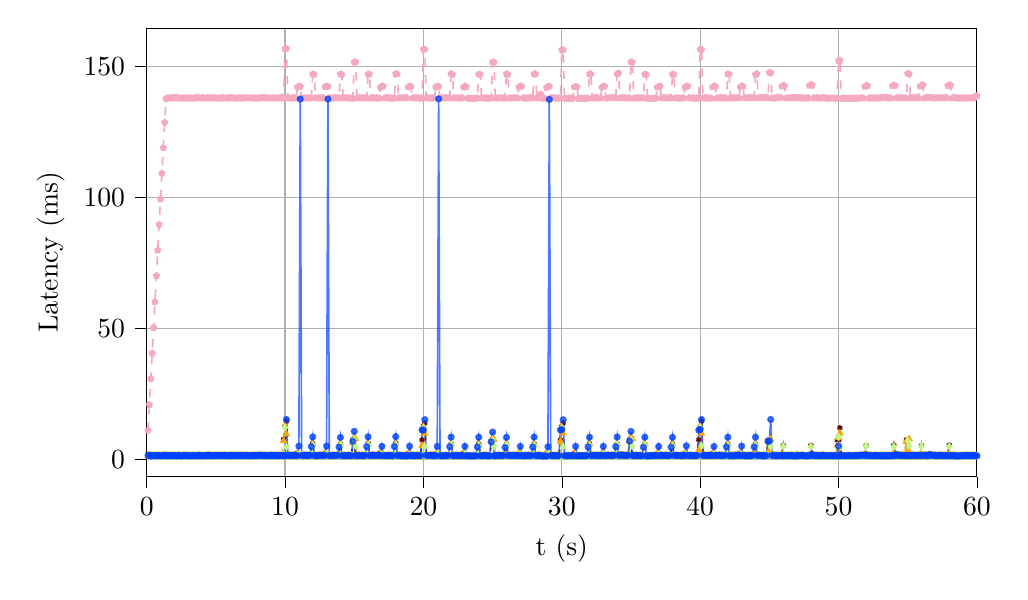
\begin{tikzpicture}

\definecolor{blue064255}{RGB}{0,64,255}
\definecolor{darkgrey176}{RGB}{176,176,176}
\definecolor{lightpink245169188}{RGB}{245,169,188}
\definecolor{maroon971111}{RGB}{97,11,11}
\definecolor{orange}{RGB}{255,165,0}
\definecolor{palegreen190247129}{RGB}{190,247,129}

\begin{axis}[
height=0.6\textwidth,
tick align=outside,
tick pos=left,
width=\textwidth,
x grid style={darkgrey176},
xlabel={t (s)},
xmajorgrids,
xmin=0, xmax=60,
xtick style={color=black},
y grid style={darkgrey176},
ylabel={Latency (ms)},
ymajorgrids,
ymin=-6.4958, ymax=164.6818,
ytick style={color=black}
]
\addplot [semithick, maroon971111, dash pattern=on 1pt off 3pt on 3pt off 3pt, mark=asterisk, mark size=1, mark options={solid}]
table {%
0.1 1.678
0.2 1.508
0.3 1.543
0.4 1.532
0.5 1.53
0.6 1.506
0.7 1.51
0.8 1.519
0.9 1.512
1 1.494
1.1 1.51
1.2 1.532
1.3 1.777
1.4 1.541
1.5 1.499
1.6 1.523
1.7 1.547
1.8 1.495
1.9 1.523
2 1.523
2.1 1.524
2.2 1.632
2.3 1.499
2.4 1.518
2.5 1.523
2.6 1.526
2.7 1.485
2.8 1.538
2.9 1.506
3 1.491
3.1 1.515
3.2 1.496
3.3 1.521
3.4 1.49
3.5 1.519
3.6 1.556
3.7 1.499
3.8 1.518
3.9 1.507
4 1.483
4.1 1.506
4.2 1.542
4.3 1.491
4.4 1.54
4.5 1.508
4.6 1.483
4.7 1.507
4.8 1.522
4.9 1.534
5 1.489
5.1 1.515
5.2 1.555
5.3 1.557
5.4 1.642
5.5 1.508
5.6 1.546
5.7 1.526
5.8 1.538
5.9 1.571
6 1.551
6.1 1.835
6.2 1.572
6.3 1.629
6.4 1.598
6.5 1.585
6.6 1.642
6.7 1.553
6.8 1.59
6.9 1.57
7 1.64
7.1 1.635
7.2 1.527
7.3 1.618
7.4 1.511
7.5 1.551
7.6 1.594
7.7 1.544
7.8 1.587
7.9 1.591
8 1.576
8.1 1.567
8.2 1.589
8.3 1.505
8.4 1.543
8.5 1.483
8.6 1.551
8.7 1.588
8.8 1.516
8.9 1.527
9 1.544
9.1 1.509
9.2 1.502
9.3 1.521
9.4 1.498
9.5 1.568
9.6 1.523
9.7 1.527
9.8 1.552
9.9 7.772
10 12.647
10.1 14.619
10.2 1.529
10.3 1.516
10.4 1.53
10.5 1.506
10.6 1.59
10.7 1.489
10.8 1.522
10.9 2.519
11 1.509
11.1 1.568
11.2 1.543
11.3 1.505
11.4 1.532
11.5 1.571
11.6 1.503
11.7 1.44
11.8 1.53
11.9 1.526
12 6.135
12.1 1.507
12.2 1.53
12.3 1.53
12.4 1.498
12.5 1.575
12.6 1.536
12.7 1.759
12.8 1.528
12.9 2.615
13 1.582
13.1 1.538
13.2 1.663
13.3 1.582
13.4 1.566
13.5 1.508
13.6 1.554
13.7 1.575
13.8 1.496
13.9 1.736
14 5.99
14.1 1.485
14.2 1.507
14.3 1.549
14.4 1.545
14.5 1.525
14.6 1.466
14.7 1.516
14.8 1.518
14.9 7.47
15 8.098
15.1 1.532
15.2 1.523
15.3 1.528
15.4 1.53
15.5 1.512
15.6 1.544
15.7 1.534
15.8 1.505
15.9 1.528
16 6.128
16.1 1.544
16.2 1.534
16.3 1.515
16.4 1.514
16.5 1.528
16.6 1.502
16.7 1.511
16.8 1.522
16.9 2.581
17 1.509
17.1 1.526
17.2 1.584
17.3 1.65
17.4 1.553
17.5 1.553
17.6 1.595
17.7 1.518
17.8 1.62
17.9 1.574
18 6.231
18.1 1.53
18.2 1.51
18.3 1.61
18.4 1.573
18.5 1.508
18.6 1.535
18.7 1.484
18.8 1.592
18.9 2.463
19 1.587
19.1 1.55
19.2 1.491
19.3 1.655
19.4 1.521
19.5 1.571
19.6 1.516
19.7 1.513
19.8 1.517
19.9 7.502
20 12.724
20.1 13.962
20.2 1.539
20.3 1.547
20.4 1.509
20.5 1.562
20.6 1.541
20.7 1.54
20.8 1.502
20.9 2.337
21 1.536
21.1 1.463
21.2 1.446
21.3 1.524
21.4 1.464
21.5 1.488
21.6 1.451
21.7 1.533
21.8 1.591
21.9 1.595
22 5.96
22.1 1.524
22.2 1.51
22.3 1.524
22.4 1.548
22.5 1.54
22.6 1.524
22.7 1.511
22.8 1.496
22.9 2.427
23 1.517
23.1 1.427
23.2 1.554
23.3 1.389
23.4 1.447
23.5 1.447
23.6 1.394
23.7 1.452
23.8 1.47
23.9 1.508
24 5.945
24.1 1.516
24.2 1.476
24.3 1.517
24.4 1.461
24.5 1.532
24.6 1.493
24.7 1.484
24.8 1.508
24.9 7.188
25 7.87
25.1 1.49
25.2 1.48
25.3 1.471
25.4 1.608
25.5 1.519
25.6 1.603
25.7 1.502
25.8 1.522
25.9 1.522
26 5.897
26.1 1.493
26.2 1.5
26.3 1.509
26.4 1.55
26.5 1.528
26.6 1.596
26.7 1.564
26.8 1.52
26.9 2.439
27 1.559
27.1 1.54
27.2 1.472
27.3 1.375
27.4 1.509
27.5 1.56
27.6 1.567
27.7 1.657
27.8 1.612
27.9 1.87
28 6.022
28.1 1.522
28.2 1.608
28.3 1.731
28.4 1.578
28.5 1.537
28.6 1.458
28.7 1.456
28.8 1.448
28.9 2.359
29 1.574
29.1 1.49
29.2 1.761
29.3 1.555
29.4 1.562
29.5 1.496
29.6 1.458
29.7 1.36
29.8 1.381
29.9 7.408
30 12.616
30.1 13.907
30.2 1.361
30.3 1.371
30.4 1.373
30.5 1.377
30.6 1.425
30.7 1.354
30.8 1.398
30.9 2.457
31 1.378
31.1 1.47
31.2 1.374
31.3 1.363
31.4 1.346
31.5 1.35
31.6 1.37
31.7 1.43
31.8 1.383
31.9 1.449
32 6.092
32.1 1.537
32.2 1.525
32.3 1.503
32.4 1.562
32.5 1.542
32.6 1.503
32.7 1.485
32.8 1.53
32.9 2.45
33 1.812
33.1 1.627
33.2 1.521
33.3 1.487
33.4 1.598
33.5 1.523
33.6 1.506
33.7 1.672
33.8 1.562
33.9 1.523
34 5.983
34.1 1.498
34.2 1.727
34.3 1.532
34.4 1.742
34.5 1.575
34.6 1.504
34.7 1.497
34.8 1.592
34.9 7.588
35 8.224
35.1 1.537
35.2 1.582
35.3 1.538
35.4 1.588
35.5 1.552
35.6 1.578
35.7 1.565
35.8 1.53
35.9 1.591
36 5.966
36.1 1.403
36.2 1.357
36.3 1.369
36.4 1.404
36.5 1.35
36.6 1.414
36.7 1.396
36.8 1.387
36.9 2.351
37 1.493
37.1 1.523
37.2 1.494
37.3 1.618
37.4 1.5
37.5 1.61
37.6 1.505
37.7 1.548
37.8 1.532
37.9 1.484
38 5.961
38.1 1.527
38.2 1.502
38.3 1.522
38.4 1.592
38.5 1.47
38.6 1.518
38.7 1.613
38.8 1.64
38.9 2.58
39 1.58
39.1 1.46
39.2 1.515
39.3 1.518
39.4 1.483
39.5 1.539
39.6 1.477
39.7 1.43
39.8 1.497
39.9 7.61
40 12.59
40.1 14.605
40.2 1.521
40.3 1.627
40.4 1.538
40.5 1.557
40.6 1.576
40.7 1.615
40.8 1.54
40.9 2.368
41 1.554
41.1 1.532
41.2 1.532
41.3 1.531
41.4 1.533
41.5 1.536
41.6 1.518
41.7 1.59
41.8 1.513
41.9 1.593
42 6.034
42.1 1.599
42.2 1.572
42.3 1.61
42.4 1.849
42.5 1.525
42.6 1.712
42.7 1.736
42.8 1.607
42.9 2.545
43 1.552
43.1 1.568
43.2 1.487
43.3 1.567
43.4 1.574
43.5 1.546
43.6 1.574
43.7 1.829
43.8 1.586
43.9 1.502
44 5.836
44.1 1.603
44.2 1.553
44.3 1.604
44.4 1.556
44.5 1.517
44.6 1.539
44.7 1.722
44.8 1.555
44.9 7.41
45 1.779
45.1 1.479
45.2 1.508
45.3 1.518
45.4 1.499
45.5 1.475
45.6 1.774
45.7 1.784
45.8 1.558
45.9 1.882
46 5.342
46.1 1.545
46.2 1.68
46.3 1.493
46.4 1.523
46.5 1.525
46.6 1.504
46.7 1.742
46.8 1.621
46.9 1.713
47 1.929
47.1 1.492
47.2 1.526
47.3 1.521
47.4 1.529
47.5 1.534
47.6 1.399
47.7 1.421
47.8 1.635
47.9 1.998
48 5.406
48.1 1.491
48.2 1.593
48.3 1.616
48.4 1.533
48.5 1.604
48.6 1.586
48.7 1.557
48.8 1.862
48.9 1.573
49 1.546
49.1 1.42
49.2 1.397
49.3 1.374
49.4 1.402
49.5 1.447
49.6 1.511
49.7 1.375
49.8 1.344
49.9 7.368
50 8.425
50.1 12.128
50.2 1.389
50.3 1.385
50.4 1.491
50.5 1.355
50.6 1.397
50.7 1.393
50.8 1.395
50.9 1.398
51 1.418
51.1 1.368
51.2 1.44
51.3 1.41
51.4 1.554
51.5 1.511
51.6 1.539
51.7 1.552
51.8 1.52
51.9 2.012
52 5.33
52.1 1.452
52.2 1.481
52.3 1.476
52.4 1.512
52.5 1.526
52.6 1.495
52.7 1.528
52.8 1.496
52.9 1.531
53 1.478
53.1 1.745
53.2 1.515
53.3 1.629
53.4 1.63
53.5 1.534
53.6 1.533
53.7 1.485
53.8 1.574
53.9 1.997
54 5.428
54.1 1.506
54.2 1.642
54.3 1.527
54.4 1.521
54.5 1.559
54.6 1.528
54.7 1.505
54.8 1.506
54.9 7.547
55 1.495
55.1 1.52
55.2 1.546
55.3 1.656
55.4 1.764
55.5 1.652
55.6 1.474
55.7 1.506
55.8 1.509
55.9 1.878
56 5.276
56.1 1.558
56.2 1.543
56.3 1.626
56.4 1.488
56.5 1.51
56.6 1.677
56.7 1.53
56.8 1.528
56.9 1.546
57 1.55
57.1 1.551
57.2 1.556
57.3 1.581
57.4 1.544
57.5 1.618
57.6 1.615
57.7 1.761
57.8 1.52
57.9 2.124
58 5.534
58.1 1.497
58.2 1.541
58.3 1.487
58.4 1.58
58.5 1.504
58.6 1.477
58.7 1.374
58.8 1.575
58.9 1.5
59 1.538
59.1 1.502
59.2 1.501
59.3 1.483
59.4 1.512
59.5 1.569
59.6 1.521
59.7 1.552
59.8 1.553
59.9 1.812
60 1.511
};
\addplot [semithick, lightpink245169188, dashed, mark=pentagon*, mark size=1, mark options={solid}]
table {%
0.1 11.123
0.2 20.939
0.3 30.868
0.4 40.597
0.5 50.345
0.6 60.211
0.7 70.179
0.8 79.912
0.9 89.75
1 99.454
1.1 109.263
1.2 118.993
1.3 128.741
1.4 137.771
1.5 138.019
1.6 138.081
1.7 137.994
1.8 137.944
1.9 138.242
2 138.032
2.1 138.077
2.2 138.295
2.3 137.966
2.4 137.974
2.5 137.94
2.6 137.94
2.7 138.016
2.8 138.036
2.9 137.949
3 137.978
3.1 138.031
3.2 138
3.3 137.931
3.4 137.965
3.5 137.972
3.6 138.281
3.7 138.073
3.8 138.126
3.9 137.923
4 138.099
4.1 138.09
4.2 138.014
4.3 137.954
4.4 138.197
4.5 138.042
4.6 138.026
4.7 137.999
4.8 138.073
4.9 138.041
5 137.956
5.1 137.989
5.2 137.969
5.3 138.022
5.4 137.964
5.5 138.254
5.6 138.014
5.7 137.973
5.8 138.003
5.9 137.968
6 138.162
6.1 138.208
6.2 137.989
6.3 137.972
6.4 137.931
6.5 137.95
6.6 138.007
6.7 138.066
6.8 138.041
6.9 137.944
7 138.002
7.1 138.112
7.2 137.974
7.3 137.978
7.4 138.081
7.5 137.977
7.6 137.974
7.7 137.983
7.8 137.968
7.9 138.004
8 137.958
8.1 137.974
8.2 138.139
8.3 138.01
8.4 138.079
8.5 138.246
8.6 138.003
8.7 137.983
8.8 138.005
8.9 138.065
9 137.991
9.1 138.028
9.2 138.095
9.3 137.973
9.4 137.969
9.5 138.044
9.6 138.03
9.7 138.037
9.8 138.455
9.9 138.051
10 156.761
10.1 156.901
10.2 138.002
10.3 137.979
10.4 137.951
10.5 137.926
10.6 138.145
10.7 137.988
10.8 137.972
10.9 142.174
11 142.543
11.1 142.456
11.2 137.923
11.3 138.025
11.4 138.019
11.5 138.058
11.6 137.943
11.7 137.999
11.8 138.056
11.9 137.995
12 147.092
12.1 147.054
12.2 138.084
12.3 138.004
12.4 137.987
12.5 138.044
12.6 137.967
12.7 138.233
12.8 138
12.9 142.326
13 142.584
13.1 142.447
13.2 138.078
13.3 138.081
13.4 137.936
13.5 138.035
13.6 138.17
13.7 137.999
13.8 138.066
13.9 138.046
14 147.15
14.1 147.01
14.2 138.238
14.3 138.01
14.4 138.028
14.5 138.145
14.6 138.032
14.7 137.959
14.8 137.938
14.9 137.935
15 151.698
15.1 151.775
15.2 137.973
15.3 138.072
15.4 138.045
15.5 137.981
15.6 138.05
15.7 138.099
15.8 138.053
15.9 137.989
16 147.13
16.1 147.097
16.2 137.958
16.3 138.129
16.4 138
16.5 137.977
16.6 138.063
16.7 137.937
16.8 137.97
16.9 142.11
17 142.595
17.1 142.491
17.2 138.023
17.3 138.121
17.4 138.067
17.5 138.032
17.6 137.969
17.7 137.959
17.8 137.963
17.9 137.977
18 147.285
18.1 147.233
18.2 138.013
18.3 138
18.4 138.009
18.5 138.081
18.6 138.014
18.7 138.028
18.8 138.083
18.9 142.177
19 142.53
19.1 142.428
19.2 137.932
19.3 138.1
19.4 138.061
19.5 138.024
19.6 138.063
19.7 137.949
19.8 137.95
19.9 137.989
20 156.619
20.1 156.602
20.2 137.986
20.3 138.071
20.4 137.998
20.5 137.908
20.6 137.999
20.7 138.055
20.8 137.987
20.9 142.182
21 142.482
21.1 142.452
21.2 138.029
21.3 137.989
21.4 138.083
21.5 137.94
21.6 138.122
21.7 138.014
21.8 138.117
21.9 138.041
22 147.294
22.1 147.038
22.2 138.02
22.3 138.01
22.4 138.004
22.5 138.014
22.6 137.998
22.7 137.947
22.8 138.165
22.9 142.113
23 142.582
23.1 142.317
23.2 137.906
23.3 137.838
23.4 137.933
23.5 137.808
23.6 137.827
23.7 137.825
23.8 137.96
23.9 137.997
24 147.053
24.1 147.027
24.2 137.984
24.3 137.997
24.4 137.95
24.5 138.036
24.6 138.043
24.7 137.959
24.8 137.937
24.9 138.071
25 151.693
25.1 151.654
25.2 137.971
25.3 137.957
25.4 138.038
25.5 138.073
25.6 138.019
25.7 138.017
25.8 137.969
25.9 137.935
26 147.235
26.1 147.027
26.2 137.984
26.3 138.009
26.4 138.014
26.5 137.979
26.6 138.012
26.7 138.049
26.8 138.056
26.9 142.183
27 142.518
27.1 142.518
27.2 138.02
27.3 137.877
27.4 137.995
27.5 137.964
27.6 138.013
27.7 138.037
27.8 138.078
27.9 138.185
28 147.21
28.1 147.172
28.2 138.032
28.3 138.026
28.4 139.35
28.5 139.464
28.6 137.958
28.7 137.849
28.8 137.822
28.9 141.982
29 142.366
29.1 142.536
29.2 138.037
29.3 138.067
29.4 137.981
29.5 138.044
29.6 137.927
29.7 137.887
29.8 137.954
29.9 137.878
30 156.459
30.1 156.396
30.2 137.941
30.3 137.854
30.4 137.845
30.5 137.871
30.6 137.954
30.7 137.904
30.8 137.873
30.9 142.186
31 142.318
31.1 142.315
31.2 137.871
31.3 137.922
31.4 137.84
31.5 137.856
31.6 137.803
31.7 137.868
31.8 137.914
31.9 137.929
32 147.21
32.1 147.163
32.2 137.982
32.3 137.943
32.4 138.117
32.5 138.26
32.6 137.959
32.7 137.982
32.8 138.019
32.9 142.155
33 142.418
33.1 142.472
33.2 137.98
33.3 137.97
33.4 138.02
33.5 138.087
33.6 138.097
33.7 138.227
33.8 137.971
33.9 137.995
34 147.242
34.1 147.527
34.2 138.002
34.3 138.136
34.4 138.084
34.5 138.162
34.6 138.062
34.7 137.973
34.8 137.982
34.9 138.056
35 151.784
35.1 151.68
35.2 137.951
35.3 138.006
35.4 137.998
35.5 138.099
35.6 138.006
35.7 138.033
35.8 137.995
35.9 138.051
36 147.108
36.1 146.988
36.2 137.808
36.3 137.894
36.4 137.878
36.5 137.896
36.6 137.867
36.7 137.863
36.8 137.938
36.9 142.123
37 142.372
37.1 142.478
37.2 137.98
37.3 138.063
37.4 138.07
37.5 138.028
37.6 138.053
37.7 137.959
37.8 138.126
37.9 138.067
38 147.14
38.1 147.01
38.2 137.999
38.3 138.055
38.4 137.963
38.5 137.946
38.6 137.915
38.7 137.994
38.8 138.002
38.9 142.131
39 142.518
39.1 142.523
39.2 137.989
39.3 138.003
39.4 137.976
39.5 137.952
39.6 137.862
39.7 137.948
39.8 138
39.9 137.951
40 156.593
40.1 156.541
40.2 138.016
40.3 137.969
40.4 138.196
40.5 137.986
40.6 137.967
40.7 137.954
40.8 137.949
40.9 142.179
41 142.574
41.1 142.423
41.2 137.979
41.3 138.045
41.4 137.984
41.5 138.208
41.6 138.009
41.7 138.045
41.8 138.054
41.9 137.945
42 147.153
42.1 147.073
42.2 138.135
42.3 137.968
42.4 138.201
42.5 138.016
42.6 137.972
42.7 138.118
42.8 138.051
42.9 142.213
43 142.578
43.1 142.508
43.2 137.977
43.3 137.977
43.4 138.174
43.5 138.083
43.6 138.153
43.7 138.183
43.8 138.039
43.9 138.16
44 147.029
44.1 147.289
44.2 138.033
44.3 137.996
44.4 138.168
44.5 138.051
44.6 138.073
44.7 138.349
44.8 138.219
44.9 138.003
45 147.721
45.1 147.687
45.2 138.052
45.3 137.969
45.4 138.056
45.5 138.035
45.6 138.292
45.7 138.011
45.8 138.261
45.9 142.466
46 142.793
46.1 142.624
46.2 137.978
46.3 138.024
46.4 138.002
46.5 138.042
46.6 138.186
46.7 138.105
46.8 138.058
46.9 138.068
47 138.233
47.1 137.99
47.2 138.277
47.3 137.965
47.4 138.036
47.5 137.98
47.6 137.905
47.7 137.889
47.8 138.118
47.9 142.797
48 143.052
48.1 143
48.2 138.066
48.3 138.039
48.4 138.071
48.5 138.042
48.6 137.96
48.7 137.992
48.8 138.161
48.9 138.088
49 138.147
49.1 137.955
49.2 137.91
49.3 137.885
49.4 137.946
49.5 137.976
49.6 137.98
49.7 137.958
49.8 137.863
49.9 137.936
50 152.264
50.1 152.376
50.2 137.896
50.3 137.875
50.4 137.963
50.5 137.842
50.6 137.796
50.7 137.883
50.8 137.871
50.9 137.869
51 137.924
51.1 137.868
51.2 137.965
51.3 137.886
51.4 137.85
51.5 137.994
51.6 137.987
51.7 138.046
51.8 137.982
51.9 142.403
52 142.791
52.1 142.739
52.2 137.975
52.3 137.949
52.4 137.935
52.5 138.015
52.6 138.005
52.7 138.021
52.8 137.958
52.9 137.974
53 137.96
53.1 138.17
53.2 138.101
53.3 138.25
53.4 138.095
53.5 138.157
53.6 138.099
53.7 137.968
53.8 137.972
53.9 142.665
54 142.858
54.1 142.761
54.2 138.144
54.3 138.001
54.4 138.103
54.5 138.165
54.6 138.048
54.7 137.987
54.8 138.003
54.9 138.033
55 147.364
55.1 147.29
55.2 138.014
55.3 138.018
55.4 138.09
55.5 138.073
55.6 138.039
55.7 138.219
55.8 137.975
55.9 142.508
56 142.88
56.1 143.023
56.2 137.939
56.3 138.067
56.4 138.243
56.5 138.227
56.6 138.109
56.7 138.141
56.8 138.058
56.9 138.064
57 138.036
57.1 138.014
57.2 138.109
57.3 138.026
57.4 137.983
57.5 138.101
57.6 138.042
57.7 138.091
57.8 138.139
57.9 142.707
58 142.909
58.1 142.931
58.2 137.947
58.3 138.213
58.4 138.167
58.5 138.129
58.6 137.886
58.7 137.88
58.8 137.98
58.9 138.072
59 138.044
59.1 137.952
59.2 137.961
59.3 138.001
59.4 138.004
59.5 138.049
59.6 138.058
59.7 138.073
59.8 138.028
59.9 138.744
60 138.845
};
\addplot [semithick, orange, dashed, mark=triangle*, mark size=1, mark options={solid}]
table {%
0.1 1.477
0.2 1.563
0.3 1.483
0.4 1.487
0.5 1.486
0.6 1.497
0.7 1.518
0.8 1.514
0.9 1.512
1 1.431
1.1 1.514
1.2 1.488
1.3 1.57
1.4 1.463
1.5 1.482
1.6 1.5
1.7 1.496
1.8 1.475
1.9 1.5
2 1.471
2.1 1.506
2.2 1.518
2.3 1.524
2.4 1.478
2.5 1.466
2.6 1.469
2.7 1.456
2.8 1.457
2.9 1.489
3 1.505
3.1 1.498
3.2 1.499
3.3 1.502
3.4 1.515
3.5 1.497
3.6 1.521
3.7 1.431
3.8 1.502
3.9 1.435
4 1.424
4.1 1.446
4.2 1.466
4.3 1.529
4.4 1.513
4.5 1.487
4.6 1.522
4.7 1.446
4.8 1.506
4.9 1.484
5 1.336
5.1 1.465
5.2 1.539
5.3 1.481
5.4 1.494
5.5 1.519
5.6 1.496
5.7 1.489
5.8 1.467
5.9 1.511
6 1.477
6.1 1.477
6.2 1.513
6.3 1.516
6.4 1.495
6.5 1.506
6.6 1.52
6.7 1.517
6.8 1.503
6.9 1.532
7 1.482
7.1 1.499
7.2 1.5
7.3 1.568
7.4 1.46
7.5 1.529
7.6 1.387
7.7 1.512
7.8 1.495
7.9 1.644
8 1.483
8.1 1.504
8.2 1.487
8.3 1.511
8.4 1.536
8.5 1.555
8.6 1.456
8.7 1.49
8.8 1.481
8.9 1.464
9 1.519
9.1 1.504
9.2 1.506
9.3 1.49
9.4 1.468
9.5 1.501
9.6 1.461
9.7 1.472
9.8 1.499
9.9 7.178
10 12.802
10.1 9.653
10.2 1.483
10.3 1.5
10.4 1.457
10.5 1.478
10.6 1.492
10.7 1.516
10.8 1.483
10.9 2.419
11 1.389
11.1 1.466
11.2 1.56
11.3 1.513
11.4 1.481
11.5 1.492
11.6 1.514
11.7 1.474
11.8 1.487
11.9 1.485
12 5.963
12.1 1.522
12.2 1.417
12.3 1.494
12.4 1.519
12.5 1.496
12.6 1.52
12.7 1.499
12.8 1.495
12.9 2.424
13 1.487
13.1 1.5
13.2 1.502
13.3 1.488
13.4 1.492
13.5 1.495
13.6 1.506
13.7 1.494
13.8 1.47
13.9 1.571
14 6.141
14.1 1.505
14.2 1.474
14.3 1.489
14.4 1.506
14.5 1.535
14.6 1.501
14.7 1.472
14.8 1.533
14.9 6.336
15 8.168
15.1 7.992
15.2 1.494
15.3 1.494
15.4 1.497
15.5 1.455
15.6 1.505
15.7 1.473
15.8 1.488
15.9 1.522
16 5.96
16.1 1.486
16.2 1.516
16.3 1.48
16.4 1.493
16.5 1.579
16.6 1.472
16.7 1.505
16.8 1.512
16.9 2.365
17 1.418
17.1 1.487
17.2 1.493
17.3 1.488
17.4 1.494
17.5 1.501
17.6 1.461
17.7 1.472
17.8 1.461
17.9 1.511
18 6.042
18.1 1.444
18.2 1.469
18.3 1.52
18.4 1.465
18.5 1.454
18.6 1.465
18.7 1.424
18.8 1.517
18.9 2.305
19 1.52
19.1 1.5
19.2 1.477
19.3 1.554
19.4 1.499
19.5 1.617
19.6 1.472
19.7 1.441
19.8 1.479
19.9 5.304
20 12.564
20.1 9.978
20.2 1.498
20.3 1.51
20.4 1.509
20.5 1.493
20.6 1.474
20.7 1.496
20.8 1.478
20.9 2.434
21 1.443
21.1 1.634
21.2 1.437
21.3 1.46
21.4 1.462
21.5 1.447
21.6 1.474
21.7 1.432
21.8 1.478
21.9 1.514
22 6.041
22.1 1.469
22.2 1.467
22.3 1.497
22.4 1.501
22.5 1.522
22.6 1.476
22.7 1.53
22.8 1.488
22.9 2.578
23 1.47
23.1 1.358
23.2 1.405
23.3 1.345
23.4 1.406
23.5 1.33
23.6 1.474
23.7 1.358
23.8 1.471
23.9 1.551
24 5.859
24.1 1.462
24.2 1.464
24.3 1.5
24.4 1.467
24.5 1.49
24.6 1.493
24.7 1.442
24.8 1.479
24.9 7.02
25 7.956
25.1 7.586
25.2 1.507
25.3 1.459
25.4 1.514
25.5 1.473
25.6 1.483
25.7 1.47
25.8 1.596
25.9 1.473
26 5.926
26.1 1.466
26.2 1.54
26.3 1.475
26.4 1.463
26.5 1.481
26.6 1.491
26.7 1.459
26.8 1.509
26.9 2.518
27 1.553
27.1 1.539
27.2 1.518
27.3 1.356
27.4 1.462
27.5 1.508
27.6 1.483
27.7 1.525
27.8 1.484
27.9 1.643
28 5.921
28.1 1.509
28.2 1.459
28.3 1.748
28.4 1.509
28.5 1.505
28.6 1.362
28.7 1.343
28.8 1.349
28.9 2.45
29 1.492
29.1 1.469
29.2 1.567
29.3 1.465
29.4 1.478
29.5 1.534
29.6 1.512
29.7 1.329
29.8 1.333
29.9 6.866
30 12.453
30.1 10.051
30.2 1.374
30.3 1.329
30.4 1.308
30.5 1.382
30.6 1.325
30.7 1.372
30.8 1.369
30.9 2.309
31 1.379
31.1 1.334
31.2 1.343
31.3 1.319
31.4 1.323
31.5 1.318
31.6 1.325
31.7 1.338
31.8 1.351
31.9 1.334
32 5.986
32.1 1.433
32.2 1.522
32.3 1.522
32.4 1.508
32.5 1.491
32.6 1.503
32.7 1.408
32.8 1.452
32.9 2.534
33 1.643
33.1 1.497
33.2 1.461
33.3 1.478
33.4 1.529
33.5 1.506
33.6 1.48
33.7 1.454
33.8 1.493
33.9 1.493
34 6.055
34.1 1.597
34.2 1.55
34.3 1.483
34.4 1.798
34.5 1.523
34.6 1.487
34.7 1.507
34.8 1.461
34.9 7.15
35 8.074
35.1 7.934
35.2 1.512
35.3 1.471
35.4 1.473
35.5 1.53
35.6 1.453
35.7 1.48
35.8 1.479
35.9 1.473
36 6.035
36.1 1.373
36.2 1.372
36.3 1.34
36.4 1.32
36.5 1.373
36.6 1.349
36.7 1.391
36.8 1.377
36.9 2.438
37 1.612
37.1 1.509
37.2 1.459
37.3 1.484
37.4 1.486
37.5 1.489
37.6 1.516
37.7 1.468
37.8 1.444
37.9 1.443
38 5.874
38.1 1.493
38.2 1.459
38.3 1.448
38.4 1.427
38.5 1.377
38.6 1.432
38.7 1.451
38.8 1.495
38.9 2.424
39 1.476
39.1 1.471
39.2 1.479
39.3 1.487
39.4 1.474
39.5 1.489
39.6 1.345
39.7 1.352
39.8 1.472
39.9 3.559
40 12.737
40.1 9.995
40.2 1.516
40.3 1.541
40.4 1.471
40.5 1.514
40.6 1.533
40.7 1.467
40.8 1.487
40.9 2.528
41 1.535
41.1 1.497
41.2 1.487
41.3 1.5
41.4 1.487
41.5 1.479
41.6 1.462
41.7 1.516
41.8 1.475
41.9 1.481
42 5.944
42.1 1.54
42.2 1.478
42.3 1.45
42.4 1.61
42.5 1.487
42.6 1.495
42.7 1.721
42.8 1.53
42.9 2.405
43 1.481
43.1 1.498
43.2 1.514
43.3 1.576
43.4 1.49
43.5 1.462
43.6 1.474
43.7 1.561
43.8 1.732
43.9 1.509
44 5.916
44.1 1.604
44.2 1.45
44.3 1.486
44.4 1.458
44.5 1.46
44.6 1.721
44.7 1.424
44.8 1.528
44.9 7.246
45 3.521
45.1 7.718
45.2 1.46
45.3 1.492
45.4 1.535
45.5 1.474
45.6 1.573
45.7 1.516
45.8 1.642
45.9 1.954
46 1.416
46.1 1.457
46.2 1.482
46.3 1.543
46.4 1.499
46.5 1.487
46.6 1.523
46.7 1.497
46.8 1.479
46.9 1.799
47 1.701
47.1 1.409
47.2 1.472
47.3 1.515
47.4 1.521
47.5 1.441
47.6 1.344
47.7 1.345
47.8 1.502
47.9 1.842
48 1.493
48.1 1.483
48.2 1.507
48.3 1.51
48.4 1.491
48.5 1.509
48.6 1.467
48.7 1.478
48.8 1.633
48.9 1.632
49 1.402
49.1 1.326
49.2 1.337
49.3 1.362
49.4 1.346
49.5 1.361
49.6 1.386
49.7 1.338
49.8 1.386
49.9 5.45
50 8.359
50.1 10.063
50.2 1.322
50.3 1.339
50.4 1.459
50.5 1.285
50.6 1.331
50.7 1.432
50.8 1.329
50.9 1.306
51 1.38
51.1 1.325
51.2 1.515
51.3 1.466
51.4 1.356
51.5 1.449
51.6 1.527
51.7 1.472
51.8 1.535
51.9 1.837
52 1.531
52.1 1.494
52.2 1.491
52.3 1.506
52.4 1.464
52.5 1.398
52.6 1.475
52.7 1.506
52.8 1.47
52.9 1.457
53 1.453
53.1 1.592
53.2 1.668
53.3 1.522
53.4 1.599
53.5 1.624
53.6 1.473
53.7 1.468
53.8 1.486
53.9 1.831
54 1.419
54.1 1.499
54.2 1.711
54.3 1.483
54.4 1.486
54.5 1.641
54.6 1.482
54.7 1.441
54.8 1.464
54.9 6.949
55 3.689
55.1 7.857
55.2 1.469
55.3 1.655
55.4 1.551
55.5 1.453
55.6 1.525
55.7 1.481
55.8 1.515
55.9 2.049
56 1.505
56.1 1.649
56.2 1.488
56.3 1.485
56.4 1.49
56.5 1.514
56.6 1.802
56.7 1.459
56.8 1.487
56.9 1.486
57 1.514
57.1 1.483
57.2 1.472
57.3 1.497
57.4 1.502
57.5 1.519
57.6 1.511
57.7 1.627
57.8 1.508
57.9 1.963
58 1.543
58.1 1.463
58.2 1.472
58.3 1.477
58.4 1.646
58.5 1.39
58.6 1.421
58.7 1.47
58.8 1.506
58.9 1.497
59 1.514
59.1 1.483
59.2 1.5
59.3 1.477
59.4 1.523
59.5 1.451
59.6 1.5
59.7 1.682
59.8 1.492
59.9 1.446
60 1.458
};
\addplot [semithick, palegreen190247129, dash pattern=on 1pt off 3pt on 3pt off 3pt, mark=diamond*, mark size=1, mark options={solid}]
table {%
0.1 1.402
0.2 1.498
0.3 1.51
0.4 1.406
0.5 1.442
0.6 1.452
0.7 1.542
0.8 1.402
0.9 1.457
1 1.419
1.1 1.561
1.2 1.469
1.3 1.441
1.4 1.541
1.5 1.45
1.6 1.416
1.7 1.467
1.8 1.443
1.9 1.626
2 1.436
2.1 1.488
2.2 1.624
2.3 1.455
2.4 1.391
2.5 1.392
2.6 1.399
2.7 1.451
2.8 1.405
2.9 1.437
3 1.42
3.1 1.424
3.2 1.449
3.3 1.533
3.4 1.522
3.5 1.455
3.6 1.787
3.7 1.43
3.8 1.521
3.9 1.509
4 1.459
4.1 1.386
4.2 1.524
4.3 1.652
4.4 1.461
4.5 1.59
4.6 1.469
4.7 1.451
4.8 1.455
4.9 1.524
5 1.313
5.1 1.463
5.2 1.425
5.3 1.445
5.4 1.443
5.5 1.424
5.6 1.455
5.7 1.46
5.8 1.444
5.9 1.446
6 1.571
6.1 1.534
6.2 1.465
6.3 1.444
6.4 1.448
6.5 1.465
6.6 1.436
6.7 1.464
6.8 1.484
6.9 1.452
7 1.514
7.1 1.458
7.2 1.417
7.3 1.448
7.4 1.444
7.5 1.453
7.6 1.447
7.7 1.441
7.8 1.453
7.9 1.436
8 1.514
8.1 1.399
8.2 1.459
8.3 1.429
8.4 1.437
8.5 1.588
8.6 1.423
8.7 1.432
8.8 1.441
8.9 1.428
9 1.421
9.1 1.452
9.2 1.434
9.3 1.447
9.4 1.542
9.5 1.413
9.6 1.442
9.7 1.516
9.8 1.443
9.9 2.096
10 12.285
10.1 4.783
10.2 1.421
10.3 1.446
10.4 1.48
10.5 1.458
10.6 1.447
10.7 1.438
10.8 1.531
10.9 1.553
11 1.914
11.1 1.441
11.2 1.456
11.3 1.451
11.4 1.449
11.5 1.447
11.6 1.424
11.7 1.453
11.8 1.453
11.9 1.445
12 5.539
12.1 1.55
12.2 1.467
12.3 1.432
12.4 1.468
12.5 1.461
12.6 1.449
12.7 1.542
12.8 1.442
12.9 1.489
13 2.01
13.1 1.459
13.2 1.445
13.3 1.452
13.4 1.464
13.5 1.452
13.6 1.44
13.7 1.455
13.8 1.449
13.9 1.452
14 5.598
14.1 1.463
14.2 1.467
14.3 1.433
14.4 1.527
14.5 1.487
14.6 1.513
14.7 1.429
14.8 1.538
14.9 1.53
15 7.774
15.1 5.157
15.2 1.519
15.3 1.415
15.4 1.462
15.5 1.445
15.6 1.46
15.7 1.487
15.8 1.544
15.9 1.441
16 5.528
16.1 1.49
16.2 1.448
16.3 1.443
16.4 1.411
16.5 1.442
16.6 1.448
16.7 1.416
16.8 1.447
16.9 1.433
17 1.969
17.1 1.434
17.2 1.438
17.3 1.436
17.4 1.454
17.5 1.61
17.6 1.46
17.7 1.617
17.8 1.43
17.9 1.642
18 5.631
18.1 1.413
18.2 1.436
18.3 1.451
18.4 1.515
18.5 1.441
18.6 1.451
18.7 1.491
18.8 1.419
18.9 1.447
19 1.855
19.1 1.576
19.2 1.531
19.3 1.43
19.4 1.575
19.5 1.503
19.6 1.464
19.7 1.567
19.8 1.43
19.9 1.464
20 12.124
20.1 4.945
20.2 1.5
20.3 1.469
20.4 1.454
20.5 1.453
20.6 1.462
20.7 1.521
20.8 1.433
20.9 1.483
21 1.962
21.1 1.434
21.2 1.536
21.3 1.429
21.4 1.546
21.5 1.455
21.6 1.54
21.7 1.526
21.8 1.449
21.9 1.504
22 5.607
22.1 1.431
22.2 1.437
22.3 1.464
22.4 1.497
22.5 1.532
22.6 1.516
22.7 1.455
22.8 1.43
22.9 1.468
23 2.075
23.1 1.3
23.2 1.316
23.3 1.319
23.4 1.294
23.5 1.306
23.6 1.32
23.7 1.328
23.8 1.452
23.9 1.434
24 5.35
24.1 1.439
24.2 1.493
24.3 1.44
24.4 1.449
24.5 1.431
24.6 1.525
24.7 1.422
24.8 1.553
24.9 1.43
25 7.505
25.1 4.972
25.2 1.473
25.3 1.458
25.4 1.45
25.5 1.433
25.6 1.476
25.7 1.511
25.8 1.436
25.9 1.46
26 5.659
26.1 1.403
26.2 1.426
26.3 1.442
26.4 1.417
26.5 1.518
26.6 1.446
26.7 1.518
26.8 1.415
26.9 1.45
27 2.063
27.1 1.523
27.2 1.408
27.3 1.369
27.4 1.534
27.5 1.495
27.6 1.47
27.7 1.452
27.8 1.477
27.9 1.505
28 5.425
28.1 1.462
28.2 1.446
28.3 1.464
28.4 1.418
28.5 1.423
28.6 1.32
28.7 1.34
28.8 1.319
28.9 1.322
29 1.975
29.1 1.453
29.2 1.475
29.3 1.528
29.4 1.524
29.5 1.476
29.6 1.424
29.7 1.343
29.8 1.333
29.9 1.323
30 12.016
30.1 4.857
30.2 1.329
30.3 1.359
30.4 1.316
30.5 1.333
30.6 1.321
30.7 1.313
30.8 1.323
30.9 1.324
31 1.851
31.1 1.312
31.2 1.322
31.3 1.417
31.4 1.408
31.5 1.326
31.6 1.417
31.7 1.345
31.8 1.323
31.9 1.326
32 5.498
32.1 1.437
32.2 1.446
32.3 1.447
32.4 1.423
32.5 1.448
32.6 1.447
32.7 1.528
32.8 1.504
32.9 1.41
33 2.09
33.1 1.526
33.2 1.505
33.3 1.453
33.4 1.428
33.5 1.438
33.6 1.456
33.7 1.621
33.8 1.451
33.9 1.46
34 5.801
34.1 1.666
34.2 1.524
34.3 1.487
34.4 1.598
34.5 1.517
34.6 1.438
34.7 1.46
34.8 1.435
34.9 1.461
35 7.614
35.1 5.137
35.2 1.51
35.3 1.426
35.4 1.593
35.5 1.431
35.6 1.462
35.7 1.547
35.8 1.471
35.9 1.516
36 5.669
36.1 1.32
36.2 1.324
36.3 1.334
36.4 1.312
36.5 1.334
36.6 1.329
36.7 1.363
36.8 1.325
36.9 1.321
37 2.006
37.1 1.489
37.2 1.464
37.3 1.434
37.4 1.444
37.5 1.431
37.6 1.43
37.7 1.465
37.8 1.433
37.9 1.432
38 5.36
38.1 1.422
38.2 1.449
38.3 1.508
38.4 1.435
38.5 1.427
38.6 1.491
38.7 1.509
38.8 1.427
38.9 1.45
39 1.954
39.1 1.44
39.2 1.443
39.3 1.472
39.4 1.53
39.5 1.432
39.6 1.368
39.7 1.349
39.8 1.429
39.9 1.412
40 12.233
40.1 5.217
40.2 1.537
40.3 1.458
40.4 1.437
40.5 1.559
40.6 1.443
40.7 1.458
40.8 1.471
40.9 1.477
41 2.082
41.1 1.434
41.2 1.522
41.3 1.404
41.4 1.449
41.5 1.692
41.6 1.498
41.7 1.45
41.8 1.477
41.9 1.427
42 5.431
42.1 1.513
42.2 1.518
42.3 1.427
42.4 1.442
42.5 1.418
42.6 1.45
42.7 1.44
42.8 1.45
42.9 1.507
43 1.941
43.1 1.428
43.2 1.487
43.3 1.434
43.4 1.754
43.5 1.54
43.6 1.596
43.7 1.537
43.8 1.433
43.9 1.57
44 5.55
44.1 1.447
44.2 1.482
44.3 1.445
44.4 1.511
44.5 1.506
44.6 1.668
44.7 1.52
44.8 1.7
44.9 1.45
45 7.275
45.1 4.96
45.2 1.435
45.3 1.438
45.4 1.71
45.5 1.584
45.6 1.454
45.7 1.48
45.8 1.499
45.9 1.497
46 5.034
46.1 1.439
46.2 1.434
46.3 1.522
46.4 1.47
46.5 1.517
46.6 1.453
46.7 1.657
46.8 1.431
46.9 1.702
47 1.493
47.1 1.426
47.2 1.439
47.3 1.426
47.4 1.47
47.5 1.427
47.6 1.33
47.7 1.32
47.8 1.693
47.9 1.516
48 4.915
48.1 1.48
48.2 1.587
48.3 1.446
48.4 1.442
48.5 1.512
48.6 1.444
48.7 1.454
48.8 1.745
48.9 1.44
49 1.481
49.1 1.34
49.2 1.314
49.3 1.319
49.4 1.369
49.5 1.418
49.6 1.486
49.7 1.323
49.8 1.346
49.9 1.315
50 8.627
50.1 4.863
50.2 1.305
50.3 1.325
50.4 1.316
50.5 1.322
50.6 1.322
50.7 1.316
50.8 1.319
50.9 1.318
51 1.316
51.1 1.368
51.2 1.325
51.3 1.329
51.4 1.38
51.5 1.52
51.6 1.462
51.7 1.452
51.8 1.506
51.9 1.442
52 5.163
52.1 1.567
52.2 1.495
52.3 1.493
52.4 1.456
52.5 1.423
52.6 1.415
52.7 1.449
52.8 1.409
52.9 1.428
53 1.509
53.1 1.537
53.2 1.586
53.3 1.444
53.4 1.621
53.5 1.623
53.6 1.536
53.7 1.498
53.8 1.428
53.9 1.421
54 4.906
54.1 1.442
54.2 1.424
54.3 1.428
54.4 1.56
54.5 1.433
54.6 1.448
54.7 1.448
54.8 1.532
54.9 1.438
55 7.176
55.1 5.054
55.2 1.532
55.3 1.535
55.4 1.416
55.5 1.529
55.6 1.575
55.7 1.581
55.8 1.431
55.9 1.446
56 5.034
56.1 1.456
56.2 1.507
56.3 1.578
56.4 1.904
56.5 1.719
56.6 1.43
56.7 1.43
56.8 1.436
56.9 1.529
57 1.449
57.1 1.473
57.2 1.432
57.3 1.572
57.4 1.516
57.5 1.546
57.6 1.549
57.7 1.52
57.8 1.528
57.9 1.459
58 5.032
58.1 1.458
58.2 1.426
58.3 1.671
58.4 1.411
58.5 1.646
58.6 1.408
58.7 1.357
58.8 1.498
58.9 1.436
59 1.513
59.1 1.468
59.2 1.499
59.3 1.491
59.4 1.449
59.5 1.513
59.6 1.664
59.7 1.51
59.8 1.433
59.9 1.514
60 1.482
};
\addplot [semithick, blue064255, opacity=0.7, mark=*, mark size=1, mark options={solid}]
table {%
0.1 1.607
0.2 1.672
0.3 1.389
0.4 1.44
0.5 1.572
0.6 1.421
0.7 1.546
0.8 1.499
0.9 1.435
1 1.452
1.1 1.431
1.2 1.577
1.3 1.557
1.4 1.59
1.5 1.417
1.6 1.466
1.7 1.562
1.8 1.489
1.9 1.56
2 1.463
2.1 1.469
2.2 1.441
2.3 1.518
2.4 1.455
2.5 1.363
2.6 1.502
2.7 1.628
2.8 1.508
2.9 1.457
3 1.433
3.1 1.442
3.2 1.489
3.3 1.452
3.4 1.464
3.5 1.55
3.6 1.499
3.7 1.44
3.8 1.678
3.9 1.436
4 1.477
4.1 1.492
4.2 1.454
4.3 1.593
4.4 1.513
4.5 1.67
4.6 1.558
4.7 1.416
4.8 1.502
4.9 1.611
5 1.438
5.1 1.567
5.2 1.532
5.3 1.544
5.4 1.559
5.5 1.501
5.6 1.62
5.7 1.591
5.8 1.428
5.9 1.53
6 1.562
6.1 1.451
6.2 1.552
6.3 1.486
6.4 1.579
6.5 1.442
6.6 1.542
6.7 1.525
6.8 1.526
6.9 1.547
7 1.524
7.1 1.474
7.2 1.542
7.3 1.571
7.4 1.47
7.5 1.471
7.6 1.543
7.7 1.51
7.8 1.504
7.9 1.6
8 1.468
8.1 1.657
8.2 1.639
8.3 1.583
8.4 1.517
8.5 1.568
8.6 1.466
8.7 1.591
8.8 1.456
8.9 1.494
9 1.663
9.1 1.522
9.2 1.557
9.3 1.497
9.4 1.651
9.5 1.438
9.6 1.512
9.7 1.589
9.8 1.527
9.9 1.5
10 1.528
10.1 15.301
10.2 1.56
10.3 1.635
10.4 1.571
10.5 1.518
10.6 1.55
10.7 1.652
10.8 1.575
10.9 1.527
11 5.132
11.1 137.656
11.2 1.528
11.3 1.609
11.4 1.619
11.5 1.581
11.6 1.572
11.7 1.597
11.8 1.588
11.9 4.963
12 8.641
12.1 1.561
12.2 1.492
12.3 1.467
12.4 1.548
12.5 1.608
12.6 1.593
12.7 1.573
12.8 1.612
12.9 1.574
13 5.092
13.1 137.625
13.2 1.49
13.3 1.507
13.4 1.54
13.5 1.561
13.6 1.566
13.7 1.607
13.8 1.565
13.9 4.773
14 8.441
14.1 1.472
14.2 1.519
14.3 1.446
14.4 1.466
14.5 1.532
14.6 1.566
14.7 1.514
14.8 1.415
14.9 6.935
15 10.76
15.1 1.53
15.2 1.475
15.3 1.58
15.4 1.579
15.5 1.509
15.6 1.487
15.7 1.486
15.8 1.552
15.9 4.928
16 8.676
16.1 1.574
16.2 1.608
16.3 1.654
16.4 1.635
16.5 1.578
16.6 1.601
16.7 1.627
16.8 1.602
16.9 1.562
17 5.035
17.1 1.489
17.2 1.47
17.3 1.507
17.4 1.434
17.5 1.562
17.6 1.529
17.7 1.545
17.8 1.462
17.9 5.007
18 8.767
18.1 1.58
18.2 1.519
18.3 1.61
18.4 1.46
18.5 1.435
18.6 1.524
18.7 1.345
18.8 1.436
18.9 1.528
19 5.105
19.1 1.552
19.2 1.528
19.3 1.495
19.4 1.482
19.5 1.517
19.6 1.546
19.7 1.555
19.8 1.504
19.9 11.3
20 11.218
20.1 15.213
20.2 1.608
20.3 1.536
20.4 1.591
20.5 1.59
20.6 1.613
20.7 1.561
20.8 1.481
20.9 1.483
21 5.005
21.1 137.72
21.2 1.485
21.3 1.473
21.4 1.408
21.5 1.524
21.6 1.488
21.7 1.551
21.8 1.521
21.9 4.93
22 8.565
22.1 1.595
22.2 1.45
22.3 1.504
22.4 1.615
22.5 1.481
22.6 1.485
22.7 1.478
22.8 1.618
22.9 1.43
23 5.05
23.1 1.427
23.2 1.411
23.3 1.496
23.4 1.328
23.5 1.412
23.6 1.356
23.7 1.412
23.8 1.423
23.9 4.831
24 8.527
24.1 1.464
24.2 1.499
24.3 1.438
24.4 1.608
24.5 1.58
24.6 1.403
24.7 1.438
24.8 1.424
24.9 6.743
25 10.487
25.1 1.417
25.2 1.471
25.3 1.464
25.4 1.619
25.5 1.529
25.6 1.524
25.7 1.524
25.8 1.565
25.9 4.611
26 8.448
26.1 1.526
26.2 1.508
26.3 1.583
26.4 1.528
26.5 1.637
26.6 1.544
26.7 1.579
26.8 1.493
26.9 1.488
27 5.016
27.1 1.606
27.2 1.506
27.3 1.389
27.4 1.617
27.5 1.522
27.6 1.496
27.7 1.502
27.8 1.543
27.9 4.808
28 8.586
28.1 1.534
28.2 1.485
28.3 1.489
28.4 1.63
28.5 1.398
28.6 1.367
28.7 1.344
28.8 1.38
28.9 1.328
29 4.854
29.1 137.513
29.2 1.562
29.3 1.55
29.4 1.546
29.5 1.508
29.6 1.534
29.7 1.408
29.8 1.52
29.9 11.286
30 11.413
30.1 15.195
30.2 1.477
30.3 1.449
30.4 1.444
30.5 1.481
30.6 1.479
30.7 1.442
30.8 1.482
30.9 1.48
31 5.03
31.1 1.451
31.2 1.415
31.3 1.482
31.4 1.448
31.5 1.414
31.6 1.488
31.7 1.436
31.8 1.421
31.9 4.881
32 8.508
32.1 1.59
32.2 1.56
32.3 1.61
32.4 1.58
32.5 1.491
32.6 1.587
32.7 1.517
32.8 1.469
32.9 1.554
33 5.018
33.1 1.556
33.2 1.569
33.3 1.624
33.4 1.604
33.5 1.544
33.6 1.579
33.7 1.58
33.8 1.565
33.9 4.932
34 8.613
34.1 1.588
34.2 1.627
34.3 1.813
34.4 1.576
34.5 1.579
34.6 1.55
34.7 1.589
34.8 1.58
34.9 7.05
35 10.739
35.1 1.55
35.2 1.499
35.3 1.521
35.4 1.556
35.5 1.475
35.6 1.536
35.7 1.511
35.8 1.493
35.9 4.724
36 8.525
36.1 1.414
36.2 1.409
36.3 1.388
36.4 1.484
36.5 1.508
36.6 1.498
36.7 1.522
36.8 1.465
36.9 1.518
37 5.004
37.1 1.527
37.2 1.602
37.3 1.623
37.4 1.551
37.5 1.528
37.6 1.55
37.7 1.518
37.8 1.499
37.9 4.744
38 8.463
38.1 1.576
38.2 1.565
38.3 1.543
38.4 1.573
38.5 1.522
38.6 1.537
38.7 1.531
38.8 1.482
38.9 1.618
39 5.203
39.1 1.543
39.2 1.579
39.3 1.546
39.4 1.555
39.5 1.559
39.6 1.444
39.7 1.456
39.8 1.546
39.9 11.267
40 11.474
40.1 15.264
40.2 1.546
40.3 1.602
40.4 1.587
40.5 1.542
40.6 1.585
40.7 1.589
40.8 1.633
40.9 1.541
41 4.977
41.1 1.536
41.2 1.614
41.3 1.627
41.4 1.66
41.5 1.543
41.6 1.527
41.7 1.554
41.8 1.602
41.9 4.844
42 8.527
42.1 1.438
42.2 1.574
42.3 1.437
42.4 1.372
42.5 1.498
42.6 1.723
42.7 1.535
42.8 1.609
42.9 1.549
43 5.129
43.1 1.587
43.2 1.51
43.3 1.412
43.4 1.432
43.5 1.538
43.6 1.558
43.7 1.461
43.8 1.547
43.9 4.817
44 8.554
44.1 1.557
44.2 1.501
44.3 1.584
44.4 1.559
44.5 1.425
44.6 1.401
44.7 1.623
44.8 1.434
44.9 6.932
45 7.137
45.1 15.301
45.2 1.525
45.3 1.612
45.4 1.624
45.5 1.423
45.6 1.465
45.7 1.496
45.8 1.494
45.9 1.62
46 1.496
46.1 1.467
46.2 1.539
46.3 1.476
46.4 1.506
46.5 1.515
46.6 1.512
46.7 1.476
46.8 1.398
46.9 1.372
47 1.499
47.1 1.419
47.2 1.545
47.3 1.589
47.4 1.568
47.5 1.468
47.6 1.455
47.7 1.362
47.8 1.488
47.9 1.53
48 1.683
48.1 1.999
48.2 1.477
48.3 1.547
48.4 1.515
48.5 1.515
48.6 1.516
48.7 1.454
48.8 1.546
48.9 1.537
49 1.563
49.1 1.416
49.2 1.464
49.3 1.464
49.4 1.568
49.5 1.511
49.6 1.387
49.7 1.465
49.8 1.467
49.9 1.402
50 5.137
50.1 1.463
50.2 1.443
50.3 1.517
50.4 1.44
50.5 1.389
50.6 1.472
50.7 1.487
50.8 1.454
50.9 1.481
51 1.412
51.1 1.491
51.2 1.451
51.3 1.49
51.4 1.541
51.5 1.618
51.6 1.651
51.7 1.637
51.8 1.647
51.9 1.587
52 1.636
52.1 1.55
52.2 1.575
52.3 1.529
52.4 1.452
52.5 1.463
52.6 1.586
52.7 1.457
52.8 1.435
52.9 1.469
53 1.463
53.1 1.474
53.2 1.46
53.3 1.512
53.4 1.475
53.5 1.481
53.6 1.5
53.7 1.411
53.8 1.494
53.9 1.558
54 1.494
54.1 1.544
54.2 1.951
54.3 1.594
54.4 1.518
54.5 1.601
54.6 1.593
54.7 1.509
54.8 1.562
54.9 1.512
55 1.557
55.1 1.579
55.2 1.564
55.3 1.61
55.4 1.548
55.5 1.647
55.6 1.504
55.7 1.549
55.8 1.593
55.9 1.571
56 1.653
56.1 1.624
56.2 1.642
56.3 1.681
56.4 1.507
56.5 1.575
56.6 1.953
56.7 1.616
56.8 1.617
56.9 1.644
57 1.498
57.1 1.443
57.2 1.625
57.3 1.62
57.4 1.506
57.5 1.523
57.6 1.437
57.7 1.582
57.8 1.429
57.9 1.555
58 1.423
58.1 1.556
58.2 1.565
58.3 1.522
58.4 1.482
58.5 1.338
58.6 1.387
58.7 1.389
58.8 1.475
58.9 1.478
59 1.478
59.1 1.531
59.2 1.515
59.3 1.599
59.4 1.494
59.5 1.473
59.6 1.492
59.7 1.527
59.8 1.515
59.9 1.502
60 1.407
};
\end{axis}

\end{tikzpicture}

        \centering \small (e) \gls{hctns}: Maximum Latency Under Burst Traffic (\textit{Conf1}).
    \end{minipage}
    \hfill
    \begin{minipage}[t]{0.45\textwidth}
        \centering
        % This file was created with tikzplotlib v0.10.1.
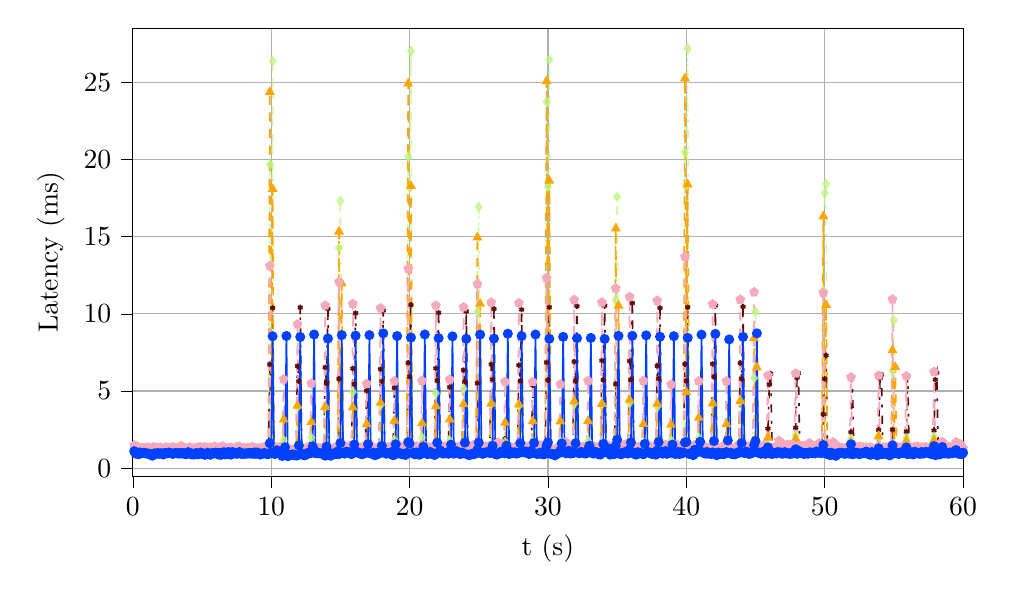
\begin{tikzpicture}

\definecolor{blue064255}{RGB}{0,64,255}
\definecolor{darkgrey176}{RGB}{176,176,176}
\definecolor{lightpink245169188}{RGB}{245,169,188}
\definecolor{maroon971111}{RGB}{97,11,11}
\definecolor{orange}{RGB}{255,165,0}
\definecolor{palegreen190247129}{RGB}{190,247,129}

\begin{axis}[
height=0.6\textwidth,
tick align=outside,
tick pos=left,
width=\textwidth,
x grid style={darkgrey176},
xlabel={t (s)},
xmajorgrids,
xmin=0, xmax=60,
xtick style={color=black},
y grid style={darkgrey176},
ylabel={Latency (ms)},
ymajorgrids,
ymin=-0.54315, ymax=28.50015,
ytick style={color=black}
]
\addplot [semithick, maroon971111, dash pattern=on 1pt off 3pt on 3pt off 3pt, mark=asterisk, mark size=1, mark options={solid}]
table {%
0.1 1.21
0.2 1.142
0.3 1.157
0.4 1.173
0.5 1.134
0.6 1.147
0.7 1.191
0.8 1.144
0.9 1.133
1 1.09
1.1 1.105
1.2 1.196
1.3 1.121
1.4 1.092
1.5 1.168
1.6 1.162
1.7 1.118
1.8 1.162
1.9 1.045
2 1.174
2.1 1.105
2.2 1.171
2.3 1.1
2.4 1.132
2.5 1.189
2.6 1.157
2.7 1.11
2.8 1.107
2.9 1.145
3 1.162
3.1 1.092
3.2 1.123
3.3 1.081
3.4 1.138
3.5 1.156
3.6 1.134
3.7 1.147
3.8 1.161
3.9 1.126
4 1.088
4.1 1.119
4.2 1.197
4.3 1.183
4.4 1.144
4.5 1.109
4.6 1.235
4.7 1.181
4.8 1.221
4.9 1.196
5 1.177
5.1 1.081
5.2 1.143
5.3 1.066
5.4 1.104
5.5 1.202
5.6 1.215
5.7 1.167
5.8 1.166
5.9 1.092
6 1.193
6.1 1.172
6.2 1.19
6.3 1.124
6.4 1.147
6.5 1.343
6.6 1.2
6.7 1.14
6.8 1.091
6.9 1.125
7 1.165
7.1 1.12
7.2 1.145
7.3 1.117
7.4 1.206
7.5 1.159
7.6 1.114
7.7 1.173
7.8 1.137
7.9 1.201
8 1.108
8.1 1.163
8.2 1.129
8.3 1.104
8.4 1.109
8.5 1.092
8.6 1.118
8.7 1.11
8.8 1.118
8.9 1.121
9 1.119
9.1 1.109
9.2 1.112
9.3 1.108
9.4 1.1
9.5 1.102
9.6 1.101
9.7 1.123
9.8 1.2
9.9 6.722
10 1.167
10.1 10.379
10.2 1.141
10.3 1.169
10.4 1.176
10.5 1.18
10.6 1.136
10.7 1.143
10.8 1.125
10.9 1.508
11 1.17
11.1 1.049
11.2 0.941
11.3 1.043
11.4 0.98
11.5 1.004
11.6 1.043
11.7 1.009
11.8 1.035
11.9 6.609
12 5.635
12.1 10.41
12.2 1.013
12.3 1.063
12.4 1.013
12.5 0.971
12.6 1.037
12.7 1.168
12.8 1.202
12.9 1.592
13 1.166
13.1 1.111
13.2 1.17
13.3 1.148
13.4 1.151
13.5 1.107
13.6 1.135
13.7 1.15
13.8 1.194
13.9 6.527
14 5.496
14.1 10.323
14.2 1.117
14.3 1.062
14.4 1.145
14.5 1.19
14.6 1.164
14.7 1.083
14.8 1.192
14.9 5.79
15 1.147
15.1 1.165
15.2 1.168
15.3 1.214
15.4 1.182
15.5 1.17
15.6 1.13
15.7 1.093
15.8 1.094
15.9 6.455
16 5.443
16.1 10.048
16.2 1.171
16.3 1.136
16.4 1.155
16.5 1.135
16.6 1.161
16.7 1.21
16.8 1.142
16.9 5.014
17 1.152
17.1 1.201
17.2 1.158
17.3 1.164
17.4 1.164
17.5 1.112
17.6 1.078
17.7 1.222
17.8 1.174
17.9 6.415
18 5.625
18.1 10.215
18.2 1.158
18.3 1.158
18.4 1.124
18.5 1.164
18.6 1.085
18.7 1.144
18.8 1.069
18.9 5.207
19 1.19
19.1 1.166
19.2 1.157
19.3 1.143
19.4 1.185
19.5 1.111
19.6 1.157
19.7 1.229
19.8 1.143
19.9 6.819
20 5.925
20.1 10.574
20.2 1.136
20.3 1.154
20.4 1.154
20.5 1.178
20.6 1.175
20.7 1.185
20.8 1.173
20.9 1.6
21 1.132
21.1 1.132
21.2 1.179
21.3 1.111
21.4 1.124
21.5 1.127
21.6 1.155
21.7 1.207
21.8 1.111
21.9 6.468
22 5.666
22.1 10.065
22.2 1.451
22.3 1.167
22.4 1.177
22.5 1.152
22.6 1.211
22.7 1.089
22.8 1.145
22.9 5.248
23 1.181
23.1 1.129
23.2 1.155
23.3 1.144
23.4 1.122
23.5 1.139
23.6 1.218
23.7 1.138
23.8 1.172
23.9 6.356
24 5.589
24.1 10.165
24.2 1.121
24.3 1.112
24.4 1.144
24.5 1.098
24.6 1.117
24.7 1.242
24.8 1.169
24.9 5.504
25 1.19
25.1 1.168
25.2 1.159
25.3 1.172
25.4 1.15
25.5 1.241
25.6 1.188
25.7 1.15
25.8 1.154
25.9 6.724
26 5.754
26.1 10.317
26.2 1.203
26.3 1.194
26.4 1.467
26.5 1.199
26.6 1.125
26.7 1.081
26.8 1.144
26.9 1.898
27 1.118
27.1 1.136
27.2 1.157
27.3 1.181
27.4 1.204
27.5 1.207
27.6 1.156
27.7 1.178
27.8 1.261
27.9 6.674
28 5.649
28.1 10.271
28.2 1.104
28.3 1.152
28.4 1.124
28.5 1.12
28.6 1.263
28.7 1.202
28.8 1.26
28.9 5.382
29 1.139
29.1 1.136
29.2 1.134
29.3 1.154
29.4 1.303
29.5 1.166
29.6 1.294
29.7 1.225
29.8 1.161
29.9 6.852
30 5.708
30.1 10.423
30.2 1.198
30.3 1.065
30.4 0.99
30.5 1.058
30.6 1.082
30.7 1.304
30.8 1.212
30.9 1.495
31 1.154
31.1 1.2
31.2 1.177
31.3 1.291
31.4 1.205
31.5 1.204
31.6 1.149
31.7 1.135
31.8 1.224
31.9 6.904
32 5.646
32.1 10.494
32.2 1.151
32.3 1.242
32.4 1.199
32.5 1.163
32.6 1.172
32.7 1.103
32.8 1.165
32.9 1.511
33 1.192
33.1 1.12
33.2 1.171
33.3 1.162
33.4 1.193
33.5 1.127
33.6 1.106
33.7 1.095
33.8 1.082
33.9 6.972
34 5.714
34.1 10.537
34.2 1.456
34.3 1.187
34.4 1.269
34.5 1.213
34.6 1.024
34.7 1.172
34.8 1.073
34.9 5.456
35 1.139
35.1 1.248
35.2 1.122
35.3 1.122
35.4 1.19
35.5 1.23
35.6 1.158
35.7 1.107
35.8 1.159
35.9 6.943
36 5.752
36.1 10.695
36.2 1.451
36.3 1.158
36.4 1.13
36.5 1.305
36.6 1.085
36.7 1.189
36.8 1.339
36.9 1.549
37 1.166
37.1 1.134
37.2 1.136
37.3 1.176
37.4 1.169
37.5 1.202
37.6 1.186
37.7 1.15
37.8 1.143
37.9 6.627
38 5.794
38.1 10.372
38.2 1.387
38.3 1.298
38.4 1.14
38.5 1.068
38.6 1.257
38.7 1.128
38.8 1.197
38.9 1.505
39 1.208
39.1 1.116
39.2 1.184
39.3 1.383
39.4 1.262
39.5 1.206
39.6 1.147
39.7 1.231
39.8 1.141
39.9 6.742
40 5.657
40.1 10.421
40.2 1.183
40.3 1.133
40.4 1.138
40.5 1.125
40.6 1.175
40.7 1.209
40.8 1.154
40.9 1.64
41 1.16
41.1 1.171
41.2 1.155
41.3 1.122
41.4 1.181
41.5 1.134
41.6 1.227
41.7 1.088
41.8 1.196
41.9 6.763
42 5.909
42.1 10.538
42.2 1.131
42.3 1.082
42.4 1.164
42.5 1.122
42.6 1.137
42.7 1.17
42.8 1.144
42.9 1.538
43 1.198
43.1 1.164
43.2 1.14
43.3 1.211
43.4 1.106
43.5 1.144
43.6 1.14
43.7 1.181
43.8 1.16
43.9 6.813
44 5.78
44.1 10.462
44.2 1.152
44.3 1.151
44.4 1.266
44.5 1.228
44.6 1.144
44.7 1.135
44.8 1.166
44.9 1.787
45 1.545
45.1 1.082
45.2 1.169
45.3 1.209
45.4 1.208
45.5 1.089
45.6 1.173
45.7 1.117
45.8 1.192
45.9 2.571
46 5.419
46.1 6.117
46.2 1.065
46.3 1.112
46.4 1.175
46.5 1.158
46.6 1.127
46.7 1.504
46.8 1.137
46.9 1.526
47 1.317
47.1 1.164
47.2 1.154
47.3 1.46
47.4 1.128
47.5 1.391
47.6 1.218
47.7 1.437
47.8 1.224
47.9 2.624
48 5.863
48.1 6.155
48.2 1.097
48.3 1.189
48.4 1.277
48.5 1.165
48.6 1.375
48.7 1.387
48.8 1.368
48.9 1.439
49 1.183
49.1 1.159
49.2 1.081
49.3 1.185
49.4 1.122
49.5 1.109
49.6 1.145
49.7 1.477
49.8 1.212
49.9 3.49
50 5.791
50.1 7.306
50.2 1.209
50.3 1.168
50.4 1.116
50.5 1.136
50.6 1.323
50.7 1.107
50.8 1.147
50.9 1.114
51 1.117
51.1 1.13
51.2 1.164
51.3 1.127
51.4 1.122
51.5 1.168
51.6 1.125
51.7 1.11
51.8 1.136
51.9 2.336
52 5.911
52.1 1.124
52.2 1.227
52.3 1.161
52.4 1.107
52.5 1.126
52.6 1.128
52.7 1.124
52.8 1.188
52.9 1.148
53 1.16
53.1 1.203
53.2 1.146
53.3 1.135
53.4 1.164
53.5 1.172
53.6 1.157
53.7 1.141
53.8 1.153
53.9 2.48
54 5.825
54.1 6.054
54.2 1.17
54.3 1.14
54.4 1.132
54.5 1.245
54.6 1.184
54.7 1.151
54.8 1.153
54.9 2.5
55 1.169
55.1 1.148
55.2 1.154
55.3 1.177
55.4 1.171
55.5 1.133
55.6 1.197
55.7 1.075
55.8 1.206
55.9 2.368
56 5.962
56.1 1.147
56.2 1.121
56.3 1.154
56.4 1.146
56.5 1.116
56.6 1.154
56.7 1.157
56.8 1.196
56.9 1.171
57 1.093
57.1 1.14
57.2 1.171
57.3 1.183
57.4 1.136
57.5 1.188
57.6 1.112
57.7 1.182
57.8 1.17
57.9 2.442
58 5.735
58.1 6.189
58.2 1.152
58.3 1.158
58.4 1.362
58.5 1.301
58.6 1.229
58.7 1.374
58.8 1.197
58.9 1.207
59 1.165
59.1 1.167
59.2 1.183
59.3 1.141
59.4 1.186
59.5 1.238
59.6 1.307
59.7 1.46
59.8 1.331
59.9 1.082
60 1.222
};
\addplot [semithick, palegreen190247129, opacity=0.7, dash pattern=on 1pt off 3pt on 3pt off 3pt, mark=diamond*, mark size=1.5, mark options={solid}]
table {%
0.1 1.161
0.2 1.076
0.3 1.163
0.4 1.033
0.5 1.091
0.6 1.07
0.7 1.141
0.8 1.051
0.9 0.977
1 1.009
1.1 1.072
1.2 1.002
1.3 1.094
1.4 0.967
1.5 1.059
1.6 1.05
1.7 1.07
1.8 1.074
1.9 0.968
2 1.064
2.1 1.021
2.2 1.016
2.3 0.972
2.4 1.059
2.5 1.049
2.6 1.035
2.7 1.058
2.8 1.02
2.9 1.073
3 1.05
3.1 1.028
3.2 1.116
3.3 1.026
3.4 1.106
3.5 1.009
3.6 1.082
3.7 1.021
3.8 1.066
3.9 1.015
4 0.992
4.1 1.08
4.2 1.055
4.3 1.036
4.4 0.985
4.5 1.075
4.6 1.095
4.7 0.986
4.8 1.089
4.9 1.047
5 0.996
5.1 1.012
5.2 1.059
5.3 1.055
5.4 1.064
5.5 1.019
5.6 1.025
5.7 1.044
5.8 1.031
5.9 1.049
6 1.066
6.1 1.027
6.2 0.989
6.3 1.032
6.4 1.055
6.5 1.091
6.6 0.994
6.7 1.075
6.8 1.006
6.9 1.051
7 1.106
7.1 1.012
7.2 1.067
7.3 1.033
7.4 1.105
7.5 1.022
7.6 1.022
7.7 1.08
7.8 1.032
7.9 1.028
8 1.028
8.1 1.065
8.2 1.102
8.3 1.09
8.4 1.01
8.5 1.003
8.6 1.032
8.7 1.15
8.8 1.046
8.9 1.008
9 1.033
9.1 1.026
9.2 0.966
9.3 1.112
9.4 1.083
9.5 0.964
9.6 1.056
9.7 1.017
9.8 1.045
9.9 19.671
10 1.068
10.1 26.387
10.2 1.068
10.3 1.121
10.4 1.028
10.5 1.044
10.6 1.043
10.7 1.078
10.8 0.916
10.9 1.807
11 1.093
11.1 0.944
11.2 0.932
11.3 0.986
11.4 0.929
11.5 0.945
11.6 0.983
11.7 0.944
11.8 0.952
11.9 3.959
12 1.05
12.1 1.001
12.2 0.888
12.3 0.947
12.4 0.897
12.5 0.954
12.6 1.095
12.7 1.128
12.8 1.057
12.9 1.971
13 1.062
13.1 0.992
13.2 1.195
13.3 1.04
13.4 1.056
13.5 0.993
13.6 1.005
13.7 1.072
13.8 1.064
13.9 3.969
14 1.102
14.1 1.033
14.2 1
14.3 0.902
14.4 1.051
14.5 1.039
14.6 1.082
14.7 1.097
14.8 1.064
14.9 14.263
15 17.307
15.1 0.999
15.2 1.123
15.3 1.122
15.4 1.045
15.5 0.994
15.6 1.068
15.7 1.049
15.8 1.053
15.9 4.937
16 1.063
16.1 1.102
16.2 1.108
16.3 1.091
16.4 1.069
16.5 1.078
16.6 1.033
16.7 1.038
16.8 1
16.9 1.559
17 1.092
17.1 1.042
17.2 1.136
17.3 1.146
17.4 1.03
17.5 0.946
17.6 0.985
17.7 1.055
17.8 1.021
17.9 4.077
18 1.047
18.1 1.053
18.2 0.993
18.3 1.04
18.4 1.05
18.5 1.045
18.6 1.106
18.7 1.001
18.8 0.907
18.9 1.827
19 1.073
19.1 1.059
19.2 1.151
19.3 1.101
19.4 1.079
19.5 1.019
19.6 1.081
19.7 1.048
19.8 1.029
19.9 20.19
20 18.166
20.1 27.021
20.2 0.997
20.3 1.101
20.4 1.134
20.5 1.124
20.6 1.007
20.7 1.062
20.8 1.117
20.9 1.99
21 1.07
21.1 1.113
21.2 1.106
21.3 0.958
21.4 1.013
21.5 1.087
21.6 1.039
21.7 1.032
21.8 1.053
21.9 4.846
22 1.066
22.1 1.098
22.2 1.217
22.3 1.119
22.4 1.025
22.5 1.101
22.6 1.099
22.7 1.096
22.8 1.063
22.9 1.78
23 1.068
23.1 1.129
23.2 1.075
23.3 1.099
23.4 1.082
23.5 1.152
23.6 1.103
23.7 1.054
23.8 1.062
23.9 5.161
24 1.253
24.1 1.007
24.2 0.976
24.3 1.001
24.4 1.018
24.5 1.055
24.6 1.107
24.7 1.065
24.8 1.006
24.9 10.126
25 16.928
25.1 1.123
25.2 1.102
25.3 1.116
25.4 1.014
25.5 0.979
25.6 1.061
25.7 1.045
25.8 1.02
25.9 4.177
26 1.108
26.1 1.078
26.2 1.09
26.3 1.074
26.4 1.162
26.5 1.065
26.6 1.033
26.7 1.101
26.8 1.109
26.9 1.705
27 1.068
27.1 1.042
27.2 1.01
27.3 1.096
27.4 1.149
27.5 1.025
27.6 1.208
27.7 1.124
27.8 1.108
27.9 4.037
28 1.065
28.1 0.985
28.2 1.039
28.3 1.018
28.4 0.992
28.5 1.048
28.6 1.047
28.7 1.081
28.8 1.146
28.9 1.731
29 1.199
29.1 1.099
29.2 1.104
29.3 1.034
29.4 1.016
29.5 1.098
29.6 1.195
29.7 0.969
29.8 1.204
29.9 23.742
30 18.237
30.1 26.475
30.2 1.051
30.3 0.901
30.4 0.98
30.5 0.909
30.6 0.967
30.7 1.177
30.8 1.065
30.9 1.715
31 1.089
31.1 1.059
31.2 1.115
31.3 1.355
31.4 1.09
31.5 1.179
31.6 1.082
31.7 0.962
31.8 1.202
31.9 4.163
32 1.124
32.1 1.192
32.2 1.092
32.3 1.19
32.4 1.063
32.5 1.092
32.6 1.096
32.7 1.06
32.8 1.048
32.9 1.773
33 1.092
33.1 1.03
33.2 1.134
33.3 1.305
33.4 1.103
33.5 1.028
33.6 1.102
33.7 1.148
33.8 1.074
33.9 4.137
34 1.211
34.1 1.328
34.2 1.249
34.3 1.059
34.4 1.312
34.5 1.004
34.6 0.972
34.7 1.188
34.8 0.981
34.9 10.909
35 17.58
35.1 1.299
35.2 1.004
35.3 1.054
35.4 1.108
35.5 1.101
35.6 1.144
35.7 1.1
35.8 1.073
35.9 4.219
36 1.109
36.1 1.019
36.2 1.281
36.3 0.968
36.4 1.043
36.5 1.127
36.6 1.059
36.7 1.112
36.8 1.075
36.9 1.64
37 1.038
37.1 1.016
37.2 1.149
37.3 1.145
37.4 1.038
37.5 1.098
37.6 1.026
37.7 1.038
37.8 1.1
37.9 3.962
38 1.035
38.1 1.057
38.2 1.206
38.3 1.354
38.4 1.14
38.5 1.296
38.6 1.402
38.7 1.155
38.8 1.047
38.9 1.795
39 0.972
39.1 1.074
39.2 1.237
39.3 1.318
39.4 1.168
39.5 1.087
39.6 1.09
39.7 1.068
39.8 0.982
39.9 20.453
40 18.33
40.1 27.18
40.2 1.064
40.3 1.067
40.4 1.033
40.5 1.068
40.6 1.168
40.7 1.268
40.8 1.08
40.9 1.976
41 1.107
41.1 1.141
41.2 1.088
41.3 1.154
41.4 1.039
41.5 1.062
41.6 0.991
41.7 1.033
41.8 1.019
41.9 4.198
42 0.999
42.1 1.142
42.2 0.928
42.3 1.004
42.4 1.003
42.5 1.104
42.6 1.062
42.7 0.996
42.8 1.061
42.9 1.631
43 1.011
43.1 1.095
43.2 1.016
43.3 1.011
43.4 1.063
43.5 0.967
43.6 1.095
43.7 1.145
43.8 1.049
43.9 4.343
44 1.047
44.1 1.054
44.2 1.091
44.3 1.057
44.4 1.055
44.5 1.092
44.6 1.02
44.7 1.069
44.8 1.126
44.9 5.83
45 10.14
45.1 1.022
45.2 0.982
45.3 1.047
45.4 1.29
45.5 1.115
45.6 1.109
45.7 1.03
45.8 1.124
45.9 1.901
46 1.074
46.1 1.126
46.2 0.979
46.3 1.067
46.4 1.095
46.5 1.02
46.6 1.094
46.7 1.21
46.8 1.164
46.9 1.139
47 1.003
47.1 1.071
47.2 1.087
47.3 1.054
47.4 1.115
47.5 1.157
47.6 1.017
47.7 1.113
47.8 1.125
47.9 2.134
48 1.224
48.1 1.061
48.2 1.091
48.3 1.063
48.4 1.031
48.5 1.186
48.6 1.142
48.7 1.331
48.8 1.2
48.9 1.204
49 1.056
49.1 1.038
49.2 1.047
49.3 1.015
49.4 1.171
49.5 1.108
49.6 1.04
49.7 1.134
49.8 1.032
49.9 11.51
50 17.823
50.1 18.411
50.2 1.114
50.3 1.083
50.4 0.939
50.5 1.141
50.6 1.147
50.7 1.039
50.8 0.971
50.9 0.989
51 1.095
51.1 1.12
51.2 1.071
51.3 0.993
51.4 1.134
51.5 1.086
51.6 1.076
51.7 1.077
51.8 1.164
51.9 1.899
52 1.051
52.1 1.109
52.2 1.046
52.3 0.971
52.4 1.146
52.5 1.042
52.6 1.054
52.7 1.049
52.8 1.025
52.9 1.084
53 1.052
53.1 1.061
53.2 1.012
53.3 1.128
53.4 1.049
53.5 1.013
53.6 1.002
53.7 0.98
53.8 0.996
53.9 2.088
54 0.991
54.1 1.02
54.2 1.062
54.3 1.125
54.4 1.053
54.5 0.998
54.6 1.051
54.7 0.986
54.8 1.019
54.9 6.323
55 9.586
55.1 1.013
55.2 1.104
55.3 1.026
55.4 1.047
55.5 1.035
55.6 1.091
55.7 1.075
55.8 1.011
55.9 1.925
56 1.019
56.1 1.157
56.2 1.004
56.3 1.057
56.4 1.032
56.5 1.106
56.6 1
56.7 1.141
56.8 0.978
56.9 1.009
57 1.116
57.1 1.036
57.2 1.032
57.3 1.076
57.4 1.054
57.5 1.054
57.6 1.106
57.7 0.994
57.8 1.059
57.9 2.029
58 1.071
58.1 1.083
58.2 1.045
58.3 1.061
58.4 1.433
58.5 1.139
58.6 1.205
58.7 1.169
58.8 1.146
58.9 1.063
59 1.084
59.1 1.066
59.2 1.045
59.3 1.026
59.4 1.084
59.5 1.375
59.6 1.089
59.7 1.173
59.8 1.052
59.9 1.04
60 1.115
};
\addplot [semithick, orange, dashed, mark=triangle*, mark size=1.5, mark options={solid}]
table {%
0.1 1.167
0.2 1.085
0.3 1.061
0.4 1.053
0.5 1.024
0.6 1.102
0.7 1.06
0.8 1.054
0.9 1.043
1 1.014
1.1 1.01
1.2 1.01
1.3 1.014
1.4 1.063
1.5 1.044
1.6 1.088
1.7 0.983
1.8 1.001
1.9 1.032
2 0.985
2.1 0.996
2.2 0.993
2.3 1.104
2.4 0.992
2.5 0.986
2.6 1.118
2.7 1.036
2.8 1.013
2.9 1.055
3 1.096
3.1 1.041
3.2 1.062
3.3 1.024
3.4 1.108
3.5 1.084
3.6 1.054
3.7 1.058
3.8 1.021
3.9 1.06
4 1.09
4.1 1.064
4.2 1.04
4.3 1.041
4.4 1.039
4.5 1.036
4.6 1.027
4.7 1.077
4.8 1.087
4.9 1.05
5 1.054
5.1 1.051
5.2 1.015
5.3 1.009
5.4 1.026
5.5 0.994
5.6 1.062
5.7 1.094
5.8 1.09
5.9 1.014
6 1.068
6.1 1.038
6.2 1.077
6.3 1.084
6.4 1.06
6.5 1.056
6.6 1.097
6.7 1.092
6.8 1.039
6.9 1.003
7 1.036
7.1 1.118
7.2 1.049
7.3 1.055
7.4 1.071
7.5 1.041
7.6 1.021
7.7 1.064
7.8 1.042
7.9 0.988
8 1.013
8.1 0.994
8.2 0.973
8.3 1.026
8.4 1.071
8.5 1.038
8.6 1.033
8.7 0.974
8.8 1.075
8.9 0.986
9 0.956
9.1 1.054
9.2 1.022
9.3 1.031
9.4 0.963
9.5 1.066
9.6 1.111
9.7 1.031
9.8 1.089
9.9 24.368
10 1.124
10.1 18.088
10.2 1.034
10.3 1.026
10.4 1.02
10.5 1.059
10.6 1.038
10.7 1.049
10.8 1.015
10.9 3.147
11 0.991
11.1 0.873
11.2 0.869
11.3 0.911
11.4 0.919
11.5 0.96
11.6 0.89
11.7 0.869
11.8 0.867
11.9 4.053
12 0.982
12.1 1.009
12.2 0.854
12.3 0.834
12.4 0.921
12.5 0.912
12.6 1.07
12.7 1.008
12.8 1.077
12.9 2.981
13 0.954
13.1 1.041
13.2 1.007
13.3 1.11
13.4 1.033
13.5 1.016
13.6 1.041
13.7 1.194
13.8 1.029
13.9 3.955
14 1.013
14.1 0.991
14.2 0.966
14.3 0.906
14.4 1.01
14.5 1.006
14.6 1
14.7 1.055
14.8 1.033
14.9 15.325
15 1.068
15.1 11.96
15.2 1.033
15.3 1.008
15.4 1.053
15.5 1.015
15.6 1.023
15.7 1.038
15.8 0.997
15.9 3.936
16 1.005
16.1 1.046
16.2 1.262
16.3 1.008
16.4 1.007
16.5 1.023
16.6 1.073
16.7 1.042
16.8 1.008
16.9 2.841
17 1.044
17.1 1.103
17.2 1.016
17.3 0.952
17.4 0.989
17.5 0.989
17.6 1.005
17.7 1.02
17.8 1.025
17.9 4.239
18 1.03
18.1 1.083
18.2 1.025
18.3 1.062
18.4 1.058
18.5 1.086
18.6 1.071
18.7 1.043
18.8 0.989
18.9 3.08
19 1.033
19.1 1.018
19.2 1.073
19.3 1.024
19.4 1.033
19.5 1.032
19.6 1.065
19.7 1.049
19.8 1.05
19.9 24.92
20 1.088
20.1 18.28
20.2 0.975
20.3 1.069
20.4 1.052
20.5 1.029
20.6 1.106
20.7 0.985
20.8 1.092
20.9 2.914
21 1.058
21.1 0.994
21.2 1.064
21.3 1.042
21.4 1.046
21.5 0.984
21.6 1.045
21.7 1.053
21.8 1.089
21.9 4.021
22 1.067
22.1 0.997
22.2 1.033
22.3 1.112
22.4 1.055
22.5 1.052
22.6 1.004
22.7 0.976
22.8 1.017
22.9 3.16
23 1.083
23.1 1.024
23.2 1.036
23.3 1.005
23.4 1.054
23.5 1.099
23.6 0.964
23.7 1.05
23.8 1.02
23.9 4.143
24 1.07
24.1 0.992
24.2 1.055
24.3 0.961
24.4 0.972
24.5 0.987
24.6 1.149
24.7 1.047
24.8 1.052
24.9 14.937
25 1.008
25.1 10.651
25.2 1.228
25.3 1.045
25.4 1.078
25.5 1.013
25.6 1.062
25.7 1.029
25.8 1.065
25.9 4.168
26 1.066
26.1 0.974
26.2 1.078
26.3 1.03
26.4 1.146
26.5 1.126
26.6 1.04
26.7 1.027
26.8 1.072
26.9 2.941
27 1.024
27.1 1.056
27.2 0.986
27.3 1.005
27.4 1.058
27.5 1.014
27.6 1.072
27.7 1.068
27.8 1.059
27.9 4.127
28 1.032
28.1 0.998
28.2 1.11
28.3 1.203
28.4 1.087
28.5 1.061
28.6 1.061
28.7 1.088
28.8 1.356
28.9 3.04
29 1.285
29.1 1.067
29.2 0.971
29.3 1.136
29.4 1.113
29.5 1.05
29.6 1.081
29.7 1.243
29.8 1.042
29.9 25.072
30 1.072
30.1 18.614
30.2 1.008
30.3 0.898
30.4 0.961
30.5 0.902
30.6 0.965
30.7 0.999
30.8 1.096
30.9 3.03
31 1.044
31.1 1.138
31.2 1.164
31.3 1.047
31.4 1.037
31.5 1.224
31.6 1.035
31.7 1.006
31.8 1.008
31.9 4.334
32 1.029
32.1 1.056
32.2 1.086
32.3 1.031
32.4 1.067
32.5 1.054
32.6 1.217
32.7 1.034
32.8 1.079
32.9 3.051
33 1.01
33.1 1.249
33.2 1.025
33.3 1.15
33.4 1.34
33.5 0.985
33.6 1.034
33.7 0.996
33.8 1.129
33.9 4.159
34 1.005
34.1 1.378
34.2 1.201
34.3 1.239
34.4 1.099
34.5 0.919
34.6 1.013
34.7 1.031
34.8 0.956
34.9 15.526
35 0.975
35.1 10.531
35.2 0.995
35.3 1.006
35.4 1.048
35.5 1.038
35.6 1.24
35.7 1.435
35.8 1.083
35.9 4.428
36 1.111
36.1 1.05
36.2 1.287
36.3 1.125
36.4 1.005
36.5 1.15
36.6 1.178
36.7 1.232
36.8 1.081
36.9 2.861
37 1.022
37.1 1.049
37.2 1.022
37.3 1.226
37.4 1.085
37.5 1.02
37.6 1.092
37.7 1.026
37.8 1.017
37.9 4.176
38 1.173
38.1 1.269
38.2 1.177
38.3 0.99
38.4 1.062
38.5 0.978
38.6 1.026
38.7 1.064
38.8 1.121
38.9 2.809
39 1.05
39.1 1.074
39.2 1.082
39.3 1.067
39.4 1.126
39.5 1.044
39.6 1.036
39.7 1.02
39.8 1.074
39.9 25.249
40 4.929
40.1 18.381
40.2 1.011
40.3 1.117
40.4 1.024
40.5 1.122
40.6 1.011
40.7 1.251
40.8 1.183
40.9 3.263
41 1.216
41.1 1.157
41.2 1.052
41.3 1.068
41.4 1.042
41.5 1.071
41.6 1.038
41.7 1.019
41.8 0.915
41.9 4.193
42 1.059
42.1 1.048
42.2 0.968
42.3 1.05
42.4 1.093
42.5 1.093
42.6 1.066
42.7 1.037
42.8 1.049
42.9 2.848
43 1.1
43.1 0.975
43.2 1.043
43.3 1.065
43.4 1.019
43.5 1.017
43.6 0.999
43.7 1.106
43.8 1.163
43.9 4.335
44 1.037
44.1 1.207
44.2 0.98
44.3 1.035
44.4 0.997
44.5 1.103
44.6 1.006
44.7 1.018
44.8 0.991
44.9 8.425
45 1.088
45.1 6.524
45.2 1.121
45.3 1.029
45.4 1.003
45.5 1.048
45.6 1.046
45.7 1.055
45.8 1.097
45.9 1.974
46 1.028
46.1 1.013
46.2 0.989
46.3 1.03
46.4 1.016
46.5 0.988
46.6 1.278
46.7 1.104
46.8 1.223
46.9 1.156
47 1.029
47.1 1.019
47.2 1.173
47.3 1.098
47.4 1.314
47.5 1.168
47.6 1.094
47.7 1.284
47.8 1.062
47.9 1.915
48 1.087
48.1 1.285
48.2 1.039
48.3 1.411
48.4 1.067
48.5 1.2
48.6 1.032
48.7 1.217
48.8 1.062
48.9 1.147
49 1.085
49.1 0.984
49.2 1.003
49.3 1.038
49.4 1.361
49.5 1.19
49.6 1.049
49.7 1.053
49.8 1.06
49.9 16.315
50 1.098
50.1 10.577
50.2 1.008
50.3 1.034
50.4 0.955
50.5 1.03
50.6 1.063
50.7 1.194
50.8 1.066
50.9 1.069
51 1.029
51.1 1.039
51.2 1.022
51.3 1.014
51.4 1.01
51.5 1.008
51.6 1.056
51.7 1.054
51.8 1.016
51.9 1.666
52 0.97
52.1 1.026
52.2 0.993
52.3 1.023
52.4 1.043
52.5 1.031
52.6 1.049
52.7 1.036
52.8 1.052
52.9 1.049
53 1.117
53.1 1.009
53.2 1.051
53.3 1.018
53.4 1.046
53.5 1.015
53.6 1.001
53.7 1.062
53.8 0.957
53.9 2.052
54 1.016
54.1 1.02
54.2 1.047
54.3 1.062
54.4 1.026
54.5 1.041
54.6 1.045
54.7 1.005
54.8 1.004
54.9 7.636
55 1.082
55.1 6.55
55.2 1.034
55.3 1.061
55.4 0.994
55.5 1.049
55.6 1.067
55.7 1.007
55.8 0.983
55.9 1.774
56 1.028
56.1 1.045
56.2 0.985
56.3 1.016
56.4 1.055
56.5 1.097
56.6 1.009
56.7 1.043
56.8 1.135
56.9 0.953
57 1.092
57.1 1.063
57.2 1.084
57.3 1.072
57.4 1.018
57.5 1.005
57.6 1.097
57.7 1.104
57.8 1.097
57.9 1.809
58 1.069
58.1 1.039
58.2 1.059
58.3 1.08
58.4 1.123
58.5 1.277
58.6 1.465
58.7 1.277
58.8 1.062
58.9 1.042
59 1.051
59.1 1.098
59.2 1.048
59.3 1.01
59.4 1.1
59.5 1.124
59.6 1.231
59.7 0.968
59.8 1.074
59.9 0.981
60 1.066
};
\addplot [semithick, lightpink245169188, dashed, mark=pentagon*, mark size=1.5, mark options={solid}]
table {%
0.1 1.48
0.2 1.37
0.3 1.409
0.4 1.339
0.5 1.308
0.6 1.318
0.7 1.259
0.8 1.314
0.9 1.318
1 1.282
1.1 1.341
1.2 1.32
1.3 1.247
1.4 1.231
1.5 1.363
1.6 1.328
1.7 1.316
1.8 1.319
1.9 1.244
2 1.329
2.1 1.297
2.2 1.215
2.3 1.295
2.4 1.357
2.5 1.247
2.6 1.309
2.7 1.288
2.8 1.351
2.9 1.349
3 1.316
3.1 1.265
3.2 1.333
3.3 1.262
3.4 1.341
3.5 1.454
3.6 1.335
3.7 1.281
3.8 1.284
3.9 1.264
4 1.27
4.1 1.35
4.2 1.262
4.3 1.298
4.4 1.248
4.5 1.288
4.6 1.321
4.7 1.337
4.8 1.358
4.9 1.336
5 1.318
5.1 1.339
5.2 1.353
5.3 1.33
5.4 1.291
5.5 1.314
5.6 1.319
5.7 1.309
5.8 1.302
5.9 1.412
6 1.291
6.1 1.302
6.2 1.278
6.3 1.34
6.4 1.385
6.5 1.413
6.6 1.36
6.7 1.263
6.8 1.289
6.9 1.284
7 1.296
7.1 1.328
7.2 1.293
7.3 1.271
7.4 1.269
7.5 1.36
7.6 1.363
7.7 1.393
7.8 1.309
7.9 1.287
8 1.326
8.1 1.287
8.2 1.277
8.3 1.313
8.4 1.272
8.5 1.251
8.6 1.373
8.7 1.361
8.8 1.289
8.9 1.311
9 1.278
9.1 1.281
9.2 1.276
9.3 1.317
9.4 1.319
9.5 1.369
9.6 1.326
9.7 1.305
9.8 1.267
9.9 13.1
10 1.328
10.1 1.332
10.2 1.408
10.3 1.323
10.4 1.365
10.5 1.327
10.6 1.343
10.7 1.37
10.8 1.188
10.9 5.762
11 1.297
11.1 1.268
11.2 1.155
11.3 1.212
11.4 1.208
11.5 1.148
11.6 1.195
11.7 1.121
11.8 1.242
11.9 9.32
12 1.253
12.1 1.284
12.2 1.167
12.3 1.17
12.4 1.204
12.5 1.131
12.6 1.358
12.7 1.34
12.8 1.326
12.9 5.494
13 1.327
13.1 1.329
13.2 1.286
13.3 1.327
13.4 1.309
13.5 1.313
13.6 1.282
13.7 1.28
13.8 1.347
13.9 10.544
14 1.299
14.1 1.305
14.2 1.266
14.3 1.239
14.4 1.232
14.5 1.31
14.6 1.32
14.7 1.239
14.8 1.326
14.9 12.065
15 1.375
15.1 1.305
15.2 1.291
15.3 1.425
15.4 1.359
15.5 1.311
15.6 1.424
15.7 1.301
15.8 1.391
15.9 10.651
16 1.41
16.1 1.362
16.2 1.425
16.3 1.296
16.4 1.325
16.5 1.336
16.6 1.27
16.7 1.399
16.8 1.335
16.9 5.475
17 1.325
17.1 1.338
17.2 1.38
17.3 1.41
17.4 1.312
17.5 1.262
17.6 1.252
17.7 1.289
17.8 1.383
17.9 10.367
18 1.334
18.1 1.3
18.2 1.319
18.3 1.284
18.4 1.329
18.5 1.325
18.6 1.416
18.7 1.39
18.8 1.166
18.9 5.643
19 1.259
19.1 1.288
19.2 1.407
19.3 1.415
19.4 1.397
19.5 1.35
19.6 1.344
19.7 1.362
19.8 1.355
19.9 12.918
20 1.351
20.1 1.261
20.2 1.343
20.3 1.359
20.4 1.361
20.5 1.416
20.6 1.368
20.7 1.253
20.8 1.442
20.9 5.664
21 1.365
21.1 1.443
21.2 1.285
21.3 1.356
21.4 1.342
21.5 1.343
21.6 1.321
21.7 1.367
21.8 1.27
21.9 10.535
22 1.316
22.1 1.296
22.2 1.394
22.3 1.324
22.4 1.364
22.5 1.391
22.6 1.383
22.7 1.387
22.8 1.336
22.9 5.745
23 1.379
23.1 1.266
23.2 1.377
23.3 1.27
23.4 1.348
23.5 1.39
23.6 1.347
23.7 1.351
23.8 1.285
23.9 10.429
24 1.571
24.1 1.335
24.2 1.309
24.3 1.328
24.4 1.221
24.5 1.323
24.6 1.496
24.7 1.406
24.8 1.333
24.9 11.923
25 1.305
25.1 1.278
25.2 1.276
25.3 1.311
25.4 1.341
25.5 1.403
25.6 1.292
25.7 1.414
25.8 1.394
25.9 10.737
26 1.31
26.1 1.329
26.2 1.369
26.3 1.267
26.4 1.661
26.5 1.421
26.6 1.291
26.7 1.289
26.8 1.251
26.9 5.601
27 1.349
27.1 1.334
27.2 1.302
27.3 1.373
27.4 1.279
27.5 1.312
27.6 1.342
27.7 1.431
27.8 1.37
27.9 10.698
28 1.379
28.1 1.384
28.2 1.357
28.3 1.424
28.4 1.388
28.5 1.348
28.6 1.406
28.7 1.46
28.8 1.441
28.9 5.59
29 1.492
29.1 1.426
29.2 1.311
29.3 1.302
29.4 1.474
29.5 1.401
29.6 1.452
29.7 1.352
29.8 1.386
29.9 12.32
30 1.369
30.1 1.374
30.2 1.289
30.3 1.213
30.4 1.172
30.5 1.178
30.6 1.278
30.7 1.309
30.8 1.342
30.9 5.43
31 1.5
31.1 1.381
31.2 1.409
31.3 1.688
31.4 1.332
31.5 1.382
31.6 1.354
31.7 1.378
31.8 1.291
31.9 10.904
32 1.292
32.1 1.423
32.2 1.372
32.3 1.33
32.4 1.324
32.5 1.357
32.6 1.391
32.7 1.364
32.8 1.336
32.9 5.656
33 1.343
33.1 1.328
33.2 1.313
33.3 1.415
33.4 1.388
33.5 1.27
33.6 1.341
33.7 1.273
33.8 1.269
33.9 10.74
34 1.489
34.1 1.407
34.2 1.529
34.3 1.399
34.4 1.438
34.5 1.423
34.6 1.234
34.7 1.443
34.8 1.192
34.9 11.651
35 1.293
35.1 1.441
35.2 1.245
35.3 1.357
35.4 1.386
35.5 1.504
35.6 1.33
35.7 1.489
35.8 1.636
35.9 11.097
36 1.371
36.1 1.367
36.2 1.445
36.3 1.352
36.4 1.295
36.5 1.349
36.6 1.382
36.7 1.398
36.8 1.359
36.9 5.657
37 1.352
37.1 1.362
37.2 1.311
37.3 1.459
37.4 1.313
37.5 1.334
37.6 1.355
37.7 1.332
37.8 1.314
37.9 10.854
38 1.388
38.1 1.377
38.2 1.442
38.3 1.394
38.4 1.352
38.5 1.504
38.6 1.412
38.7 1.383
38.8 1.48
38.9 5.422
39 1.311
39.1 1.375
39.2 1.289
39.3 1.525
39.4 1.456
39.5 1.347
39.6 1.384
39.7 1.406
39.8 1.357
39.9 13.695
40 1.505
40.1 1.47
40.2 1.346
40.3 1.289
40.4 1.315
40.5 1.317
40.6 1.504
40.7 1.402
40.8 1.399
40.9 5.632
41 1.56
41.1 1.571
41.2 1.466
41.3 1.298
41.4 1.278
41.5 1.295
41.6 1.324
41.7 1.363
41.8 1.321
41.9 10.629
42 1.359
42.1 1.261
42.2 1.348
42.3 1.278
42.4 1.314
42.5 1.304
42.6 1.4
42.7 1.288
42.8 1.31
42.9 5.642
43 1.355
43.1 1.304
43.2 1.324
43.3 1.286
43.4 1.263
43.5 1.287
43.6 1.285
43.7 1.352
43.8 1.54
43.9 10.922
44 1.355
44.1 1.302
44.2 1.314
44.3 1.349
44.4 1.326
44.5 1.415
44.6 1.32
44.7 1.461
44.8 1.416
44.9 11.407
45 1.317
45.1 1.311
45.2 1.24
45.3 1.389
45.4 1.336
45.5 1.358
45.6 1.469
45.7 1.402
45.8 1.38
45.9 6.006
46 1.329
46.1 1.327
46.2 1.304
46.3 1.33
46.4 1.339
46.5 1.307
46.6 1.404
46.7 1.78
46.8 1.632
46.9 1.616
47 1.351
47.1 1.343
47.2 1.298
47.3 1.523
47.4 1.41
47.5 1.499
47.6 1.497
47.7 1.532
47.8 1.416
47.9 6.135
48 1.382
48.1 1.329
48.2 1.313
48.3 1.431
48.4 1.441
48.5 1.396
48.6 1.428
48.7 1.401
48.8 1.451
48.9 1.626
49 1.315
49.1 1.252
49.2 1.29
49.3 1.314
49.4 1.341
49.5 1.417
49.6 1.621
49.7 1.475
49.8 1.385
49.9 11.356
50 1.419
50.1 1.539
50.2 1.253
50.3 1.385
50.4 1.205
50.5 1.513
50.6 1.696
50.7 1.313
50.8 1.34
50.9 1.357
51 1.394
51.1 1.317
51.2 1.294
51.3 1.291
51.4 1.284
51.5 1.284
51.6 1.337
51.7 1.292
51.8 1.277
51.9 5.892
52 1.257
52.1 1.301
52.2 1.425
52.3 1.279
52.4 1.321
52.5 1.37
52.6 1.37
52.7 1.368
52.8 1.333
52.9 1.296
53 1.348
53.1 1.244
53.2 1.258
53.3 1.352
53.4 1.279
53.5 1.283
53.6 1.255
53.7 1.25
53.8 1.294
53.9 6.002
54 1.282
54.1 1.267
54.2 1.345
54.3 1.319
54.4 1.318
54.5 1.356
54.6 1.294
54.7 1.309
54.8 1.289
54.9 10.938
55 1.317
55.1 1.27
55.2 1.32
55.3 1.376
55.4 1.284
55.5 1.334
55.6 1.348
55.7 1.35
55.8 1.357
55.9 5.963
56 1.312
56.1 1.39
56.2 1.302
56.3 1.303
56.4 1.345
56.5 1.367
56.6 1.332
56.7 1.413
56.8 1.253
56.9 1.317
57 1.342
57.1 1.345
57.2 1.31
57.3 1.361
57.4 1.335
57.5 1.304
57.6 1.288
57.7 1.362
57.8 1.298
57.9 6.248
58 1.335
58.1 1.454
58.2 1.32
58.3 1.299
58.4 1.632
58.5 1.703
58.6 1.365
58.7 1.459
58.8 1.416
58.9 1.299
59 1.379
59.1 1.357
59.2 1.328
59.3 1.331
59.4 1.428
59.5 1.688
59.6 1.352
59.7 1.535
59.8 1.548
59.9 1.407
60 1.276
};
\addplot [semithick, blue064255, mark=*, mark size=1.5, mark options={solid}]
table {%
0.1 1.101
0.2 0.947
0.3 0.949
0.4 0.903
0.5 1.017
0.6 0.955
0.7 0.993
0.8 0.995
0.9 0.979
1 0.943
1.1 0.944
1.2 0.937
1.3 0.876
1.4 0.807
1.5 0.941
1.6 0.961
1.7 0.932
1.8 0.984
1.9 0.928
2 0.956
2.1 0.96
2.2 0.888
2.3 0.98
2.4 0.961
2.5 0.979
2.6 1.014
2.7 0.987
2.8 0.951
2.9 0.929
3 0.963
3.1 0.978
3.2 0.973
3.3 0.94
3.4 0.98
3.5 0.941
3.6 0.985
3.7 0.946
3.8 0.905
3.9 0.923
4 1.04
4.1 0.961
4.2 0.899
4.3 0.943
4.4 0.881
4.5 0.96
4.6 0.98
4.7 0.896
4.8 0.927
4.9 1.011
5 0.933
5.1 0.944
5.2 0.862
5.3 0.911
5.4 1.002
5.5 0.926
5.6 0.866
5.7 0.975
5.8 0.96
5.9 0.981
6 0.999
6.1 0.989
6.2 0.874
6.3 0.981
6.4 0.865
6.5 1.014
6.6 1.032
6.7 0.887
6.8 0.939
6.9 1.048
7 0.898
7.1 0.877
7.2 1.042
7.3 1.002
7.4 0.99
7.5 0.926
7.6 0.966
7.7 1.046
7.8 0.94
7.9 0.916
8 0.95
8.1 0.927
8.2 0.968
8.3 0.943
8.4 0.982
8.5 0.938
8.6 0.975
8.7 0.933
8.8 1.022
8.9 0.924
9 1.013
9.1 0.937
9.2 0.883
9.3 0.94
9.4 0.946
9.5 0.981
9.6 0.946
9.7 0.913
9.8 0.914
9.9 1.613
10 1.026
10.1 8.544
10.2 0.934
10.3 0.929
10.4 1.163
10.5 0.974
10.6 0.986
10.7 1.051
10.8 0.789
10.9 1.105
11 1.356
11.1 8.564
11.2 0.777
11.3 0.825
11.4 0.84
11.5 0.881
11.6 0.888
11.7 0.854
11.8 0.82
11.9 0.835
12 1.476
12.1 8.498
12.2 0.937
12.3 0.86
12.4 0.831
12.5 0.86
12.6 0.976
12.7 0.967
12.8 0.98
12.9 0.99
13 1.399
13.1 8.66
13.2 0.968
13.3 1.046
13.4 0.963
13.5 0.971
13.6 0.948
13.7 0.945
13.8 0.986
13.9 0.809
14 1.397
14.1 8.397
14.2 0.998
14.3 0.805
14.4 0.906
14.5 0.949
14.6 0.926
14.7 0.919
14.8 1.083
14.9 0.911
15 1.627
15.1 8.621
15.2 1.001
15.3 0.94
15.4 1.058
15.5 1.063
15.6 1.03
15.7 0.983
15.8 0.905
15.9 0.966
16 1.531
16.1 8.584
16.2 1.062
16.3 0.988
16.4 0.952
16.5 0.929
16.6 0.904
16.7 0.991
16.8 0.981
16.9 1.013
17 1.557
17.1 8.62
17.2 0.948
17.3 0.96
17.4 1
17.5 0.835
17.6 0.876
17.7 0.992
17.8 0.953
17.9 0.992
18 1.442
18.1 8.735
18.2 1.013
18.3 0.939
18.4 0.955
18.5 0.986
18.6 0.948
18.7 1.045
18.8 0.84
18.9 0.869
19 1.548
19.1 8.559
19.2 0.978
19.3 0.979
19.4 0.912
19.5 0.899
19.6 0.912
19.7 0.855
19.8 0.991
19.9 1.682
20 1.591
20.1 8.462
20.2 0.967
20.3 1.004
20.4 0.889
20.5 1.016
20.6 0.945
20.7 0.869
20.8 0.989
20.9 0.945
21 1.393
21.1 8.66
21.2 0.977
21.3 0.908
21.4 0.975
21.5 1.052
21.6 0.921
21.7 0.928
21.8 0.851
21.9 0.925
22 1.653
22.1 8.424
22.2 1.159
22.3 1.016
22.4 0.948
22.5 0.958
22.6 0.968
22.7 1.023
22.8 0.933
22.9 1.034
23 1.525
23.1 8.54
23.2 0.938
23.3 1.034
23.4 1.097
23.5 0.989
23.6 0.933
23.7 0.926
23.8 1.012
23.9 0.955
24 1.656
24.1 8.377
24.2 0.885
24.3 0.843
24.4 0.876
24.5 0.929
24.6 0.897
24.7 0.979
24.8 0.95
24.9 1.2
25 1.662
25.1 8.654
25.2 0.952
25.3 0.93
25.4 0.995
25.5 1.024
25.6 1.02
25.7 1.053
25.8 0.977
25.9 1.081
26 1.45
26.1 8.394
26.2 0.907
26.3 0.88
26.4 0.938
26.5 0.956
26.6 1.064
26.7 0.996
26.8 1.019
26.9 0.963
27 1.454
27.1 8.711
27.2 0.915
27.3 1.049
27.4 1.017
27.5 0.972
27.6 1.03
27.7 0.947
27.8 0.954
27.9 1.012
28 1.617
28.1 8.554
28.2 1.04
28.3 1.034
28.4 1.083
28.5 1.026
28.6 0.932
28.7 0.931
28.8 1.127
28.9 1.004
29 1.637
29.1 8.66
29.2 0.92
29.3 0.961
29.4 0.935
29.5 1.018
29.6 0.927
29.7 0.889
29.8 1.079
29.9 1.464
30 1.677
30.1 8.382
30.2 0.921
30.3 0.924
30.4 0.902
30.5 0.826
30.6 0.902
30.7 0.942
30.8 0.989
30.9 1.15
31 1.602
31.1 8.508
31.2 1.076
31.3 0.964
31.4 0.985
31.5 1.125
31.6 0.948
31.7 1.066
31.8 0.974
31.9 1.009
32 1.608
32.1 8.42
32.2 0.983
32.3 0.974
32.4 1.054
32.5 1
32.6 0.98
32.7 0.948
32.8 0.972
32.9 1.221
33 1.453
33.1 8.438
33.2 0.977
33.3 0.948
33.4 1.057
33.5 1.027
33.6 0.933
33.7 0.893
33.8 0.887
33.9 1.017
34 1.572
34.1 8.368
34.2 1.046
34.3 1.02
34.4 1.273
34.5 0.879
34.6 0.938
34.7 0.946
34.8 0.91
34.9 1.452
35 1.84
35.1 8.571
35.2 0.925
35.3 0.898
35.4 1.005
35.5 0.983
35.6 1.052
35.7 0.963
35.8 0.949
35.9 1.211
36 1.665
36.1 8.576
36.2 0.986
36.3 0.89
36.4 0.882
36.5 1.035
36.6 0.978
36.7 0.986
36.8 0.941
36.9 0.904
37 1.571
37.1 8.603
37.2 1.042
37.3 1.025
37.4 0.999
37.5 0.921
37.6 0.958
37.7 0.987
37.8 0.876
37.9 1.153
38 1.701
38.1 8.514
38.2 1.076
38.3 0.937
38.4 0.987
38.5 1.113
38.6 0.926
38.7 0.99
38.8 1.023
38.9 1.007
39 1.523
39.1 8.551
39.2 0.914
39.3 0.983
39.4 1.054
39.5 0.909
39.6 1.03
39.7 0.966
39.8 1.018
39.9 1.669
40 1.698
40.1 8.442
40.2 0.927
40.3 0.924
40.4 1.012
40.5 0.842
40.6 1.186
40.7 0.995
40.8 1.09
40.9 1.222
41 1.712
41.1 8.649
41.2 1.006
41.3 1.004
41.4 0.938
41.5 1.049
41.6 0.938
41.7 0.971
41.8 0.916
41.9 1.019
42 1.761
42.1 8.698
42.2 0.839
42.3 1.013
42.4 0.93
42.5 0.923
42.6 0.982
42.7 0.905
42.8 0.936
42.9 1.042
43 1.796
43.1 8.34
43.2 1.002
43.3 0.905
43.4 0.949
43.5 0.893
43.6 0.948
43.7 0.972
43.8 1.052
43.9 1.013
44 1.627
44.1 8.506
44.2 0.979
44.3 1.058
44.4 1.049
44.5 0.927
44.6 0.945
44.7 0.962
44.8 1.009
44.9 1.49
45 1.76
45.1 8.735
45.2 0.998
45.3 1
45.4 0.932
45.5 0.997
45.6 1.083
45.7 0.926
45.8 0.967
45.9 1.348
46 0.962
46.1 0.954
46.2 0.921
46.3 0.964
46.4 0.985
46.5 0.952
46.6 1.04
46.7 1.002
46.8 1.019
46.9 0.938
47 0.951
47.1 1.041
47.2 0.954
47.3 0.966
47.4 0.949
47.5 0.918
47.6 1.001
47.7 0.952
47.8 1.009
47.9 1.225
48 0.925
48.1 1.124
48.2 0.973
48.3 1.028
48.4 0.994
48.5 0.915
48.6 0.965
48.7 0.987
48.8 0.931
48.9 1.019
49 1.015
49.1 0.965
49.2 0.994
49.3 0.961
49.4 1.08
49.5 1.026
49.6 0.995
49.7 1.026
49.8 0.97
49.9 1.498
50 1.057
50.1 0.998
50.2 0.904
50.3 0.977
50.4 0.842
50.5 0.993
50.6 0.908
50.7 0.929
50.8 0.801
50.9 0.959
51 0.971
51.1 0.998
51.2 0.989
51.3 0.988
51.4 0.935
51.5 0.942
51.6 0.989
51.7 0.946
51.8 0.951
51.9 1.55
52 0.897
52.1 1.005
52.2 0.938
52.3 0.993
52.4 0.981
52.5 0.9
52.6 0.951
52.7 0.977
52.8 0.968
52.9 0.982
53 1.075
53.1 0.954
53.2 0.901
53.3 0.863
53.4 1.043
53.5 0.956
53.6 0.983
53.7 0.972
53.8 0.833
53.9 1.287
54 1.069
54.1 0.931
54.2 0.914
54.3 0.98
54.4 0.933
54.5 1.004
54.6 0.964
54.7 0.829
54.8 0.902
54.9 1.48
55 0.999
55.1 0.976
55.2 1.021
55.3 0.934
55.4 0.93
55.5 1.013
55.6 1.029
55.7 0.973
55.8 0.992
55.9 1.347
56 0.898
56.1 0.986
56.2 1.036
56.3 0.918
56.4 0.886
56.5 1.067
56.6 1.018
56.7 0.991
56.8 0.944
56.9 0.93
57 1.047
57.1 0.944
57.2 0.972
57.3 1.059
57.4 1.005
57.5 1.036
57.6 1.011
57.7 0.906
57.8 1.014
57.9 1.434
58 0.842
58.1 1.027
58.2 0.949
58.3 0.884
58.4 0.992
58.5 1.369
58.6 0.958
58.7 0.959
58.8 0.991
58.9 0.943
59 0.938
59.1 1.024
59.2 0.969
59.3 0.986
59.4 1.02
59.5 1.172
59.6 1.045
59.7 0.925
59.8 0.949
59.9 0.911
60 1.001
};
\end{axis}

\end{tikzpicture}

        \centering \small (f) \gls{hctns}: Maximum Latency Under Burst Traffic (\textit{Conf2}).
    \end{minipage}
    \caption{Experiment C: \gls{hctns} and \cite{Lin2021} model performance under burst traffic.}
    \label{expc-conf}
\end{figure*}
}

\rev{During \textit{Interval 1}, traffic classes transmit at a constant rate without generating traffic bursts. As depicted in Figs.~\ref{expc-conf}b and \ref{expc-conf}c, both models show similar bandwidth behavior, with BE traffic using all the remaining bandwidth not consumed by other traffic classes. However, the latency behavior (Figs.~\ref{expc-conf}d and~\ref{expc-conf}e) for the BE traffic differs, since the~\cite{Lin2021} model, in addition to accepting background traffic from other flows, admits 100\,Mbps of BE traffic. As a result, the low priority queue is congested and BE packets experiment a high latency. In contrast, since \gls{hctns} incorporates a global policer that limits the traffic admitted at the transport network's ingress, it ensures that the accepted traffic does not exceed the queues' capacity. This results in low latency values, similar to the rest of the flows.}

During \textit{Interval 2}, traffic bursts are generated for all defined traffic classes. \rev{In the~\cite{Lin2021} model, the bursts accepted from all traffics are classified as ``green", being forwarded to the highest priority queue. As the priority queue is not saturated, these packets are transmitted. When bursts are accepted, the highest priority queue uses a higher transmission rate, which reduces the transmission rate of the lower priority queue, causing the downward spikes in bandwidth in Fig.~\ref{expc-conf}b.} In \gls{hctns}, a very close bandwidth behavior (Fig.~\ref{expc-conf}c) is observed, accepting a similar amount of burst packers. In this case, the configured \gls{cbs} and \gls{pbs} values allow the defined amount of bytes to ingress the \gls{tn}, while the excess traffic is queued in the \gls{htb} ingress queue. If this queue becomes full, any additional packets are discarded. As explained in Section~\ref{sec:proposal}.\ref{subsec:proposal-finegraine}, when traffic burst control is enabled and bursts are accepted by the class policers (or the slice policer for \gls{urllc} traffic), both the slice and global policers may temporally have ``negative'' tokens. Consequently, BE traffic is not admitted by the ingress policer until the slice policer's bucket recovers the tokens it owed restoring a positive balance. Until the global policer's bucket is not fully recovered, BE traffic cannot borrow bandwidth beyond the \gls{embb} slice's \gls{cir}. As a result, during burst periods, the bandwidth available to the BE traffic shows also temporary downward spikes. This mechanism ensures that, while packets arriving at rates exceeding the \gls{cir} defined in the global policer may be temporally accepted, the average bandwidth will remain within the defined limits. 

\rev{As shown in Fig.~\ref{expc-conf}d, traffic bursts impact the latency of all flows when using the~\cite{Lin2021} model. This is because the accepted burst packets (``green") are forwarded to the highest priority queue, regardless of the traffic flow to which they belong. As a result, all burst traffic from the flows undergoes similar treatment. For example, all  traffic flows experience a similar maximum latency,  around 15\,ms. Packets marked as ``yellow" are forwarded to the lowest priority queue, which is congested. Since BE traffic continuously enters the lowest priority queue at 100\,Mbps and the lowest priority queue cannot transmit a packet if there are packets in the highest priority queue, most ``yellow" packets from the burst will be discarded due to queue overflow. For the same reason, ``yellow" packets, such as those from \gls{urllc} traffic, experience latencies exceeding 130 ms, which is unacceptable.}

In \gls{hctns}, as illustrated in Fig.~\ref{expc-conf}e, traffic bursts also have a significant impact on the latency. While the average rate at which packets arrive at the \gls{pe}1 input port does not exceed the output port capacity, bursts temporarily surpass this capacity. This causes packets to be enqueued at the \gls{pe}1 output port, resulting in delays. However, since the average accepted rate remains below the global policer's \gls{cir}, which is adjusted to the available network capacity, packets do not accumulate over time in these queues. Therefore, it is crucial to properly dimension the queue sizes to handle bursty traffic effectively, preventing packet loss. 

Since \gls{urllc} traffic is assigned to \gls{tn} \gls{qos} class A, which has a priority queue, its latency remains unaffected  by traffic bursts from the other \gls{tn} \gls{qos} classes. However, \gls{urllc} bursts impact the delay in the \gls{drr} queues, as these queues must wait for the priority queues to empty before transmitting packets. Additionally, the latency experienced by traffic classes in \gls{tn} \gls{qos} classes with \gls{drr} queues is also influenced by the bursts in other \gls{drr} queues. For example, when bursts from the telemetry and VC traffic classes are transmitted, the latency experienced by BE and \gls{tod} video traffic increases. As will be explained below, different coarse-grained resource control configurations can be applied to manage and control this latency. \rev{Unlike \cite{Lin2021}, all traffic accepted by the policers from the same \gls{tn} \gls{qos} class receives the same treatment, achieving \gls{urllc}, video, telemetry, and VC latencies of under 9\,ms, 13\,ms, 21\,ms, and 21\,ms, respectively. The BE queue is not saturated, so latency values remain within these ranges.}

\rev{In \textit{Interval 3}, when there are no \gls{urllc} traffic bursts, the latency perceived by the other traffic classes decreases in both models. In the~\cite{Lin2021} model, fewer packets are queued in the highest priority queue, which reduces the waiting time for packets arriving at this queue. As a result, the maximum latency values achieved are around 12\,ms. Additionally, although some packets are marked as ``yellow'', the saturation of the lowest priority queue prevents any ``yellow" packets from entering the buffer. This explains why the latency spikes have disappeared. However, as the lowest priority queue remains saturated, the latency perceived by BE traffic does not change.}

\rev{In \gls{hctns}, the latency experienced by traffic classes assigned to \gls{tn} \gls{qos} classes with an allocated \gls{drr} queue is still influenced by bursts from other \gls{drr} queues. However, the latency values decrease to under 8\,ms for video and under 15\,ms for telemetry and VC. Since the BE queue is not saturated, its latency values also remain within these ranges.}

In \gls{hctns}, as expected, all the traffic classes sharing a \gls{tn} \gls{qos} class experiment similar latency values, due to the \gls{phb} applied at the output port through the coarse-grained resource control configuration. 

Fig.~\ref{expc-conf}f shows how different coarse-grained resource control configurations (quantum values)  affect latencies experienced by the traffic classes. The \textit{Conf2} configuration, as shown in Table~\ref{tab:expc-params}, was used to obtain the following results. 

This new configuration of the coarse-grained resource control mechanism allows the \gls{tn} \gls{qos} class B (which carries \gls{tod} video) to have a higher transmission rate, compared to the previous configuration. As a result, its queued packets are transmitted earlier, reducing the latency experienced. For example, a maximum latency of 12.89\,ms was measured in the experiment shown in Fig.~\ref{expc-conf}e, compared to 10.69\,ms in the experiment shown in Fig.~\ref{expc-conf}f. The other \gls{tn} \gls{qos} classes now have a lower transmission rate than in the previous coarse-grained resource control configuration, which leads to increased latency for those traffic classes.

\rev{Despite both models achieving similar bandwidth results, in \gls{hctns}, by adjusting the quantum values in the coarse-grained resource control configuration, the latency experienced by the traffic of a \gls{tn} \gls{qos} class can be controlled. As observed throughout all the experiments, when using \gls{hctns}, packets experience queuing delays under burst traffic conditions. However, even in these cases, unlike with the~\cite{Lin2021} model, this latency can be controlled by \gls{hctns}. In \gls{hctns}, the latency of \gls{urllc} traffic is solely influenced by the traffic bursts of this \gls{tn} \gls{qos} class, while the latency in the remaining traffic classes depends not only on the accepted \gls{urllc} traffic bursts, but also on the bursts accepted by other \gls{tn} \gls{qos} classes. In contrast, in the~\cite{Lin2021} model, the latency of each traffic flow is influenced by the bursts of other traffic flows, including BE traffic, when some of its packets are classified as ``yellow". This causes the~\cite{Lin2021} model to perform worse than \gls{hctns}.}

\section{Conclusions}
\label{sec:conclusion}

In this paper, we have proposed \gls{hctns}, a slicing model  that employs a three-level hierarchical \gls{htb} to implement a fine-grained resource control mechanism at the ingress node of the transport network. This mechanism is combined with coarse-grained resource control in the transport network nodes to allow meeting the bandwidth and latency requirements of services defined within the slices, even in worst-case scenarios and with bursty traffic, while achieving a high level of network bandwidth sharing both within and across slices. One of the strengths of \gls{hctns} is that all the traffic admitted to be processed in the transport network is treated with \gls{qos} guarantees, not only the traffic under the guaranteed bitrate but also traffic exceeding it (up to certain limit), and even for limited traffic bursts.

\rev{In real deployments, each network segment operates independently as an administrative domain, meaning that end-to-end performance depends on the specific traffic management solutions implemented in each segment. HCTNS ensures that the latency, bandwidth, and packet loss requirements defined in the SLAs are met within the transport network, contributing to their fulfillment end-to-end. While HCTNS does not impact the performance of the RAN or core network, it is essential for maintaining service guarantees in the transport network and, by extension, across the entire system.}

\rev{An experimental platform combining virtual and physical network elements has allowed us to verify that \gls{hctns} outperforms not only the model being standardized by the \gls{ietf}, but also a state-of-the-art reference approach, in terms of bandwidth utilization, latency and traffic burst control.}  



As future steps for this research, we believe that centralized policies are needed to guarantee end-to-end delay bounds in the transport network. In addition, models are required to translate these policies into configurations for data plane functions in the transport network equipment. This includes the establishment and configuration of IPv6 tunnels based on \gls{sr} with routing algorithms driven by \gls{qos} metrics.  


\bibliography{ojcoms}

\begin{IEEEbiographynophoto}{Jane Doe}
    Biography text here without a photo.
\end{IEEEbiographynophoto}

\begin{IEEEbiography}[
    %{\includegraphics[width=1in,height=1.25in,clip,keepaspectratio]{}}
    ]{IEEE Publications Technology Team}
    In this paragraph you can place your educational, professional background and research and other interests.\end{IEEEbiography}

\end{document}